\documentclass{outline-of-mechanics}

\begin{document}
\widowpenalty0
\clubpenalty0

% 封面

\includepdf{body/F00-Frontpage.pdf}

% 标题页
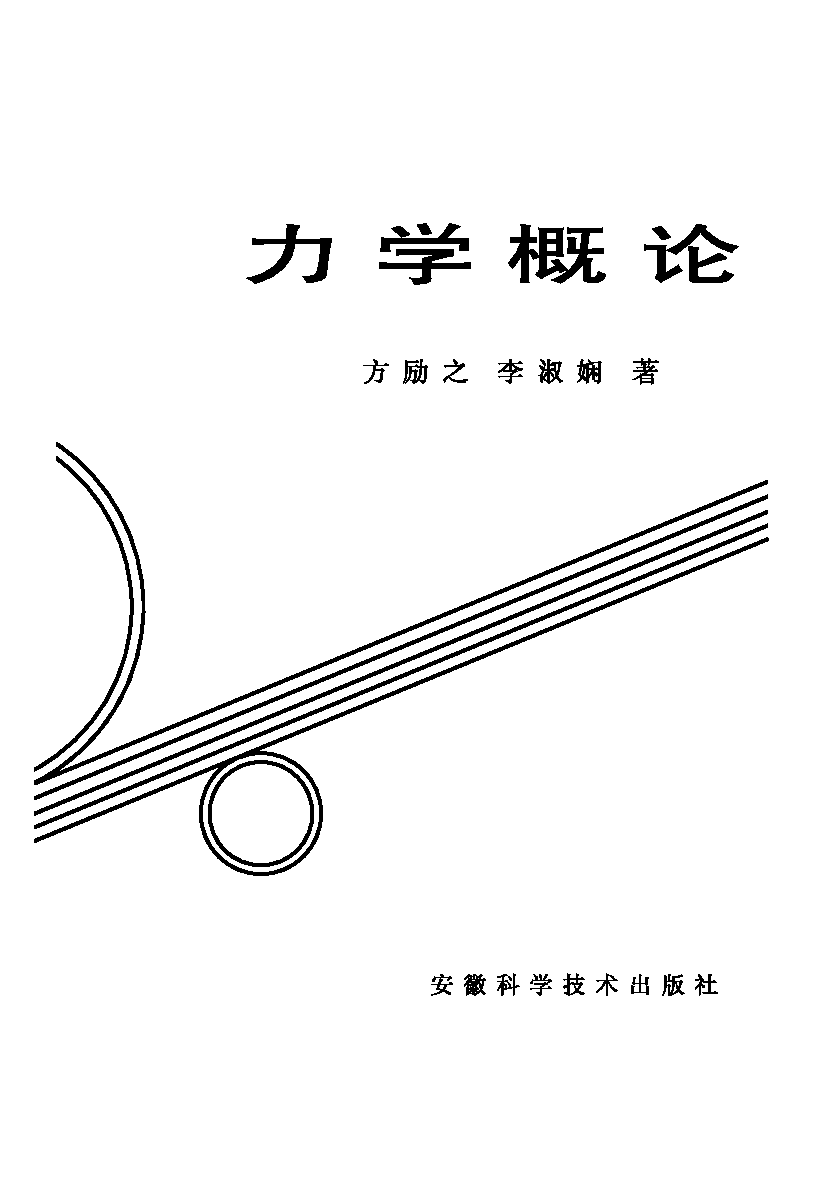
\includepdf{body/F01-Titlepage.pdf}

% 出版信息页
% 出版信息页
\begin{center}
  \zihao{4}\fangsong\mbox{}

  \mbox{}\label{publish}\pdfbookmark{出版页}{publish}

  责任编辑:张晓红

  封面设计:陈治黄

  \vfill \heiti{力~~学~~概~~论}

  \normalsize \kaishu{方励之~~李淑娴}

  \normalfont{} *

  安徽科学技术出版社出版

  \zihao{-5} (合肥市跃进路1号)

  \normalsize 安徽省%
  \hspace{0.2em}\raisebox{-0.5mm}{
\includegraphics[width=4em]{icon/xinhuabokestore}}\hspace{0.2em}%
  发行~~安徽新华印刷厂印刷

  *

  \zihao{6}开本:850$\times$1168~~1/32~~印张:12.5~~字数:309,000

  1986年1月第一版~~~~1986年1月第一次印刷

  印数00,001—5,000

  \normalsize 统一书号:13200$\cdot$68~~~~定价:2.5元
\end{center}
\thispagestyle{empty}
\clearpage


% 内容提要
% 内容提要
\begin{center}
  \begin{minipage}{8.4cm}\vspace{3cm}
    \begin{center}\heiti{内~容~提~要}\end{center}
    \zihao{-5}
    \hspace{2em}本书是根据作者在中国科学技术大学及北京大学讲授普通物理的
    力学部分讲稿整理而成的。其特点是强调用物理的前沿发展去改进基础物理教
    学,即用现代物理的观点去选择课程的内容,去表现概念和规律。因此,书中
    包括一些在传统的教材中没有的内容,如牛顿宇宙学等,对许多传统的内容,
    也采取新的讲授法,使之能与当代物理的进展相呼应。另外。由于力学是物理
    学的入门和基础,所以本书也注意物理方法的阐述,这对于初学物理的学生是
    有益的。书中还附有一些习题及答案。

    \hspace{2em}本书可作为综合大学及师范院校的普通物理力学教材,也可供大
    专院校物理教师及物理教学研究工作者参考。
  \end{minipage}
\end{center}
\thispagestyle{empty}
\clearpage

% 序言
\setcounter{page}{1}
\pagestyle{foreword}
\null\vspace{1em}
\begin{center}
    \label{foreword}\pdfbookmark{序}{foreword}
  \zihao{4}\heiti{序}

  \null{}
\end{center}
\fangsong\normalsize

这本书原是一份普通物理课程的力学讲义,它曾在中国科学
技术大学沿用多年,也曾在北京大学教授过数次。

普通物理中的力学,是相当难教的,凡是教授过这门课的老
师,大都有此体会。一方面,力学是整个物理学的基石,它包含
许多基本的观念、方法和理论,需要学生极为准确地加以掌握,
以备后继学习之用,另一方面,初入大学的学生,往往看轻力学,
误认为新的内容不多,似乎在中学里都已学过,结果力学反而被
疏忽了。

这种局面迫使一些教师采用理论力学的方法来教授普通物理
力学。这样做,确实可以解决前述问题的第二方面,学生不再感
到“似曾相识”了。随着教和学二者的提高,原属理论力学的部
分内容的确可以逐渐放到普通物理中来。但是,我们觉得,若仅
限于这一途径改进教学,还不能或不完全能解决问题的第一个方
面——力学是整个物理的一块基石。

基石到底在哪里起了基石的作用?基石到底如何起了基石的
作用?显然,这些“哪里”,这些“如何”只有从物理的当代发
展以及前沿研究的角度,才能看得清楚。这就是说,如果我们企图
从“物理的基石”这一标准来组织教学,它至少有以下两方面的
含义:一是不断用新的现代的观点去整理老的内容,一是不断用新
的前沿的重要成果来充实基础。事实上,不同时代的教材的差别,
最清楚地表现在这些方面。上进的标准,也就是我们在编写这本
教材时,尝试着击追求的。也许有的地方达到了,也许有的地方%分页处
并未达到。无论成功或失败,它都是我们的追求的记录。

为了使用上的方便,书中编辑了一些例题,每章末也附有一
些思考题和习题。由于北京大学物理系和中国科学技术大学物理
教研室已编有《物理学习题集》(人民教育出版社,1980),为了不
重复太多,本书中的例题和习题只是标志性的。在教学上需要更
多习题时,可以参考上述的习题集。

在使讲义变成这本书的过程中,得到过员汝槐同志的协助,
谨致谢意。

\null{}

\hspace{6.8cm}\zihao{-4}\kaishu{作~~~者}

\mbox{}

\hspace{7cm}\normalfont{} \zihao{-5}1984年4月\normalsize
\clearpage

% 目录
\clearpage
\setcounter{page}{1}
\tableofcontents

% 正文
\clearpage
\pagestyle{heading}
\setcounter{page}{1}
% 公式与上下文本距离调整
\setlength\abovedisplayskip{3pt plus 3pt minus 1pt}
\setlength\belowdisplayskip{3pt plus 3pt minus 1pt}

% 绪论
\ctexset{chapter={number={\quad},name={绪,论}}}
\chapter{—— ~ 物理世界的统一}\label{chp:0}
\ctexset{chapter={number={\chinese{chapter}},name={第,章}}}

物理学的兴起,是从经典力学开始的。在经典力学之前,人类
的文明中虽然已有不少具有物理价值的发现和发明,但是并不存
在一门独立的物理学。因此,我们在学习经典力学的时候,首先
应当了解:为什么经典力学成了物理学的起点?经典力学在整个
物理学中占据着怎样的地位?

爱因斯坦曾经这样来概括牛顿力学的历史地位;“古代希腊
伟大的唯物主义者坚持主张,一切物质事件都应当归结为一系列
的有规律的原子运动,而不允许把任何生物的意志作为独立的原
因。而且无疑笛卡尔曾按他自己的方式重新探索过这一问题。但
是,在当时,它始终不过是一个大胆的奢望,一个哲学学派的成
问题的理想而已。在牛顿之前,还没有什么实际的结果来支持那
种认为物理因果关系有完整链条的信念。”

这句话的意思是,物理学依赖于一种基本的信念:物理世界
存在着完整的因果链条,即自然界是统一的。牛顿力学则是体现
这种信念的第一个成功的范例。

从牛顿力学的创建到现在,已经有三百多年了,物理学已经
大大发展了,远远超过了经典力学原有的水平。但是,就物理学
的最基本的追求和物理学的总目标来说,却一直没有变化。经典
力学时代的追求和目标,可以说时至今日仍然是整个物理学的追
求和目标。这个最基本的追求和目标,就是自然界的统一。的确,
从整个物理学的发展中,可以看到一条鲜明的主线。这就是执着%分页点
地追求宇宙的统一,找寻支配宇宙万物的最基本最统一的规律。

相信存在统一,努力寻求统一,如果仅仅作为一种自然观,
早在古代已经有了。老子的《道德经》中写有:“道生一、一生
二、二生三、三生万物。”这就是中国古代的一种统一观,它完
全可以与爱因斯坦所提及的古希腊的哲学相媲美。不过,无论在
古代中国或古希腊,统一观都只是一种哲学思辨。

牛顿的力学和古代的哲学不同,它不是思辨地坚持统一观,
而是发展了寻找统一的有效的物理方法。牛顿在他的最重要的力
学著作《自然哲学的数学原理》中阐明了他采用的方法。他在前
言中写道;“我奉献这一作品。作为哲学的数学原理,因为哲学
的全部责任似乎在于——从运动的现象去研究自然界中的力,然
后从这些力去说明其他的现象。”\sbfootnote{牛顿这段话里的
  “哲学”一词,实际含义相当于今天的“科学”或“物理学”。}这就是
说,寻求统一的出发点不是思辨而应是运动现象。自然界中的运动
现象是多种多样的,物理学的责任就在于寻找支配这些现象的统一的力。

今天的物理学,仍然大体地沿袭着牛顿所开创的研究途径。
寻找统一的力,或统一的相互作用。因此,几乎所有基本的物理
理论都称做某种力学,如牛顿力学、电动力学、色动力学等等。
每一种新的力学的确立,都标志着我们在追求统一的逾程上达到
了一个新的水平。

为了更具体地表达上述的论述。我们利用表1。表1左边列举
的是自然界中的种种运动现象,也就是物理学的研究对象。天体
的运行和地面物体的运动是人首先看到或接触到的,随后才有时
间、空间的概念,所以时空也是一种物理研究的对象,另一类现
象是电、磁和光,所有这些物理对象。在二十世纪之前,人们都
已知道了。二十世纪以来,又逐渐证实或发现一些新的对象。如
原予、原子核、核子以及夸克等。

\clearpage
表\ref{tab:00.01}~的其余部分就表示物理学在寻求统一,寻求完整的因果
链条上一些重要的阶段。
牛顿的力学和万有引力定律,是物理学上第一次大的统一。
在牛顿之前,传统的观念认为支配天体运行和支配地面物体运动
的规律是不相同的,有所谓天界和世俗两个世界之分。然而,牛
顿发现,天上行星和月亮的运动,实际上和地面落体运动遵从相
同的规律,它们都是由引力引起的。这样,牛顿就用他的力学打
破了天界和世俗的界限,找到了两个世界的统一。牛顿称引力为
万有引力,就是强调这种统一。

第二次大的统一,是由十九世纪的麦克斯韦完成的。他建立
了电磁理论,使电、磁及光学现象得到统一。这就是电动力学。

很快发现,牛顿的力学和麦克斯韦的电磁学这两大领域在时
\begin{table}[!h]
  \centering
  \caption{物理学发展中的统一$^*$}\label{tab:00.01}
  \begin{tabular}{c}
    \toprule \vspace{-1em}            \\
    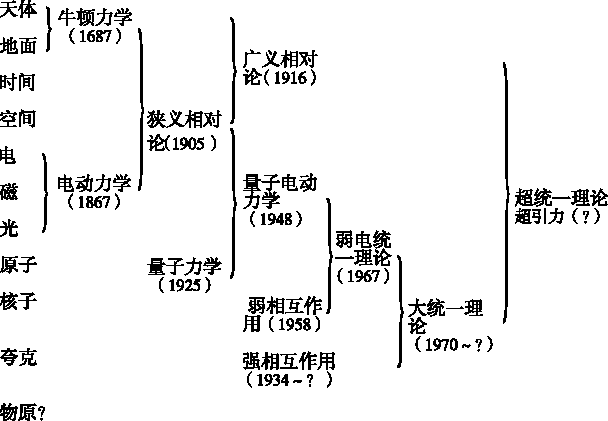
\includegraphics{figure/tab00.01} \\
    \bottomrule
    \zihao{6}* 括号中的数字表示相应的理论建立的年代;有问号的表示尚未完成。
  \end{tabular}
\end{table}
\clearpage\noindent 空观上是很不协调的。在前者中,各种匀速运动是平权的,但却
假定有绝对空间或绝对速度存在。相反,在后者中,有一个地位
特殊的速度,即光速,但却始终测不出这个特殊的速度是相对于
哪一个绝对空间而言的。爱因斯坦抛弃了绝对空间观念,使电磁
学、力学在新的时空观的基础上达到了协调和统一。

爱因斯坦还曾企图把引力和电磁力二者统一起来,但他的努
力没有成功。然而,他却找到了能与麦克斯韦电磁理论相协调的
引力理论——广义相对论。

作为引力理论的广义相对论和作为电磁理论的麦克斯韦理论
构成了我们今夭称为经典物理学的理论基础。

与经典物理相对的是量子论。量子力学最初是作为原子、分
子的统一的力学而发展起来的。这种新的力学统一地解释了原子、
分子的各种光谱现象,统一地解释了元素周期表,统一地解释了
各种不同分子的键合。

在将量子力学扩展到电磁场时,遇到了困难,这本质上是由
于电磁场是相对论性的。直到四十年代末,发展了所谓重整化方
法才巧妙地解决了上述的困难,使量子论与电磁理论能得以统一,
产生了量子电动力学。

到六十年代末,我们已经得到了如下的物理世界的图象。宇
宙中的所有物理对象可以分成两大类,一类称为“物质”,如夸
克、电子、$\mu$子等等,另一类称为“相互作用”,如引力、电磁力
等等。在目前的宇宙中,有四种基本的相互作用,按它们的强度
顺序排列是:核子参与的强相互作用,荷电粒子参与的电磁相互
作用,核子及电子、中微子参与的弱相互作用,以及任何粒子都
参与的引力相互作用。可以简单地说,宇宙间的一切运动和变化。
都可以统一为这四种“力”的作用。但是,追求统一的物理学,
似乎认为这种状况仍然不够统一。

1967年,温伯格和萨拉姆再次着眼于统一,先后提出了电磁
相互作用和弱相互作用的统一理论。随后的一系列实验证明他们
的统一理论是正确的。

这一新的成功,促使许多人去找寻把电磁作用、弱作用及强
作用都包含在内的统一理论,通常称为“大统一理论”。建立这
种理论的工作还没有完成,这是正在研究的领域。

如果大统一能够顺利完成,下一步的统一就是要把引力也统
一在内了。引力是物理学最早讨论的一种基本的力。但是,它与
其他力的统一最难,因为引力有一系列很特别的性质。例如这种
力只有引力却无斥力。就是这种特别性质之一。

企图把引力与其他力统一起来的工作,称为超统一的研究。
目前还没有得到有实际意义的结果。它是今天的物理学的一个前
沿。实现超统一的一个可能是用超引力理论,这种理论中的统一
有一个很有趣的特点,即它把物理学中传统的“物质”与“相互
作用”之间的界限也打破了。

总之,从牛顿力学开始,物理学就在寻找宇宙的统一,我们
希望找到控制着万事万物运动的极少的几个基点。只有从这个角
度我们才容易看清经典力学在整个物理学中的地位和作用,也才
能全面地了解学习经典力学对于学习整个物理学的意义和作用。


% 第一章
\chapter{时间,空间和运动学}\label{chp:01}

\section[时间]{\makebox[5em][s]{时间}}\label{sec:01.01}

描写物体的运动,要用时间和空间这两个概念。因此,我们
先来对时间、空间本身作一些分析。

时间和空间可以说是最平凡的概念了,因为在日常生活中也
常常用到它们。不过,若问什么是时间?什么是空间?却又不容易
找到恰当的答案。其实,这是两个很难的问题。尽管有不少关于
时间和空间的定义,但大都不能令人满意。一种或许可以接受的
说法是:时间、空间是物理事件之间的一种次序,时间用以表述
事物之简的顺序,空间用以表述事件相互之间的位形。

没有满意的“严格”的理论定义,并不妨碍时间和空间二者
在物理中的使用。因为,物理学是一门基于实验的科学,在考查
物理学的概念或物理量的时候,首先应当注意它与实验之间是否
有明确的、不含糊的关系。对于时间和空间这两个基本概念来说,
首要的问题似不是去追究它们的“纯粹”定义,而是应当了解它
们是怎样量度的。

量度时间,通常是用钟和表。然而,钟和表并不是测量时间
的唯一的工具。原则上。任何具有重复性的过程或现象,都可以
作为测量时间的一种钟。自然界里有许多重复性的过程,其中有
一些我们早已把它们当作计时标准了。例如,太阳的升没表示天;
四季的循环称作年;月亮的盈亏是农历的月。其他的循环过程,
如双星的旋转、人体的脉搏、吊灯的摆动,分子的振动等等,也
都可以用作测时的工具。

更一般地说,只要知道了某个物理现象随时间的变化,尽管
它不是重复性的过程,也可以用来测定时间。譬如,我们能从一
个人的容貌估计出他的年龄,因为容貌这个量与时间之间有确定
的关系。这个例子虽然很普通,但某些有用的测时方法与此是很
相似的。在确定星体的年龄时,常常就是根据星体的颜色。

钟的种类很多,但有好有坏。比较两个人的脉搏,就会发现
它们之间经常有明显的快慢波动,所以,人的脉搏不是一种好钟,
它不够稳定。如果比较一下两个单摆的周期,就会发现它们稳定
多了。地球自转则是更稳定的钟。
\begin{figure}[!h]
  \centering
  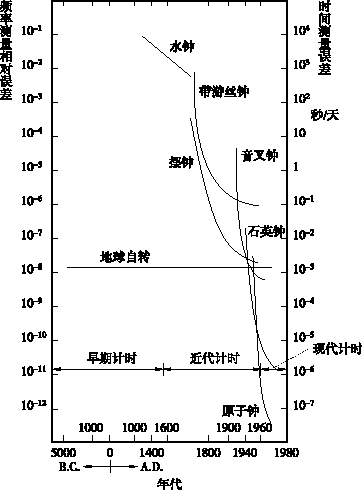
\includegraphics[height=8cm]{figure/fig01.01}
  \caption{不同年代的时间测量精度}\label{fig:01.01}
\end{figure}

\clearpage
图\ref{fig:01.01}给出不同年代用不同的钟测量时间所达到的精度。可以
看到,地球自转要比各种机械的钟都好。所以,1967年以前是用
地球自转作为标准钟。原子钟是比地球自转更加稳定的钟,现代
的精密计时都是用原子钟了。

\begin{table}[!h]
  \centering
  \caption{一些典型物理现象的时间尺度}\label{tab:01.01}
  \begin{tabular}{c}
    \toprule
    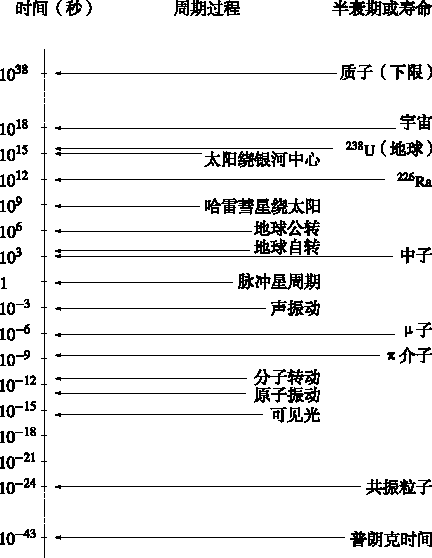
\includegraphics[width=0.8\linewidth]{figure/tab01.01} \\
    \bottomrule
  \end{tabular}
\end{table}
\clearpage
1967年10月在第十三届国际度量衡会议上通过了新的标准
钟,它对一秒的时间作如下的规定;位于海平面上的$^{133}$Cs原子
的基态的两个超精细能级在零磁场中跃迁辐射的周期$T$与$ 1 $秒的
关系为
\begin{equation*}
  1 \,\text{秒} = 9,192,631,770\,T
\end{equation*}

表\ref{tab:01.01}~列举了一些典型现象的时间尺度。目前,物理学中涉及
的最长的时间是:\num{e38}秒,它是质子寿命的下限。宇宙的年龄大约
是 \num{6e17}秒,即$ 200 $亿年。牛顿力学所涉及的时间尺度大约是
\num{e-3}$\sim$\num{e15}秒,即从声振动的周期到太阳绕银河中心转动的周期。
粒子物理的时间尺度都很小。$\mu$子的寿命是 \num{2e-6} 秒。已经算是
极长寿的了。最短寿的是一些共振粒子,它们的寿命只约有 \num{e-24}
秒。目前物理学中涉及的最小的时间是 \num{e-42}秒,称为普朗克时
间。普朗克时间被认为是最小的时间,比普朗克时间还要小的范
围内,时间的概念可能就不再适用了。

\section{芝诺佯谬和时间的度量}\label{sec:01.02}

古希腊哲学家芝诺有一个很著名的论证:跑得最快的神话英
雄阿基里斯是永远追不上跑得最慢的东西 (例如一只龟) 的。他的
论证如下:因为开始时阿基里斯是在龟的后面,所以,阿基里斯
要追上龟,他必定先要到达龟的出发点,这要用有限的时间,在
这段时间里龟必定向前跑了,到达前面的一点,而当阿基里斯再
到达这点时,龟必定又已到达更前面的一点。如此重复下去,就
是进行无穷多次,龟也总不会落在阿基里斯之后。

这个论证被称为芝诺佯谬,如何解开这个佯谬?

关键是在芝诺佯谬中用了两种不同的时间度量。按上节的讨
论,任何一种具有重复性的过程。都可以做为“钟”,用其重复
的次数来量度时间。芝诺问题中。除了“普通”钟所测得的时间
$t$,还利用了一种很特别的钟,该钟使用的重复性过程是:阿基里
斯逐次地到达龟在前一次的出发点。我们称这种钟叫芝诺钟,它
测得的时间为$t'$。

\begin{figure}[!h]
  \centering
  
\includegraphics{figure/fig01.02}
  \caption{芝诺时的定义}\label{fig:01.02}
\end{figure}

如图\ref{fig:01.02},阿基里斯和龟在开始时相距为$L$,速度分别为$v_1$及
$v_2$,并且$v_1>v_2$。如果用普通的钟,则阿基里斯将在
\begin{equation}
  t=L/\left(v_1-v_2\right)
  \label{eqn:01.02.01}
\end{equation}
时,赶上龟;当$t>L/\left(v_1-v_2\right)$时,阿基里斯就超过龟了。

图中左边的数字表示的是芝诺时$t'$。当$t'=1$时,阿基里斯到
达龟在0时的出发点;当$t'=2$时,阿基里斯到达龟在1时的出发
点。一般地,当$t'=n$时,阿基里斯到达龟在$t'=n-1$时的位置。
显然,只有当$t'\to\infty$时,阿基里斯才能逼近龟,对于任何有限的
$t'$,阿基里斯总是落在龟的后面。这就是芝诺的结论。

因此,芝诺断言:“阿基里斯永远也追不上龟。”这里“永
远”的含意是$t'\to\infty$。,即芝诺时间的无限。

现在我们来讨论普通时$t$与芝诺时$t'$之间的变换关系。不难
验证表\ref{tab:01.02} 给出的两种时间的对应。因此,一般有
{\setlength{\mathindent}{4em}
\begin{equation}\label{eqn:01.02.02}
  t=\sum_{n=0}^{t^{\prime}-1} \frac{L}{v_{1}}{\left(\frac{v_{2}}{v_{1}}\right)}^{n}=\frac{L}{v_{1}-v_{2}}\left[1-{\left(\frac{v_{2}}{v_{1}}\right)}^{t'}\right]
\end{equation}}%
或者
\begin{equation}
  t^{\prime}=\frac{1}{\ln \left(v_{2} / v_{1}\right)} \ln \left[1-\left(\frac{v_{1}-v_{2}}{L}\right) t\right]
  \label{eqn:01.02.03}
\end{equation}%
式\eqref{eqn:01.02.02}或式\eqref{eqn:01.02.03}称为芝诺变换。它给出的$t'$与t的关系。在
图\ref{fig:01.03}~中画出。

\begin{table}[!h]
  %\renewcommand\arraystretch{1.6}
  \centering
  \caption{普通时与芝诺时的关系}\label{tab:01.02}
  \zihao{-5}
  \begin{tblr}{colsep=2em,row{2-Z}={rowsep=0em},colspec={c|X}}
    \toprule
    芝诺时($t'$) & \SetCell{c}普通时($t$)                                                                                                        \\
    \midrule
    0         & 0                                                                                                                          \\[1.75ex]
    1         & $\dfrac{L}{v_1}$                                                                                                           \\[1.75ex]
    2         & $\dfrac{L}{v_1} +\dfrac{L}{v_1}\cdot\dfrac{v_2}{v_1}$                                                                      \\[1.75ex]
    \vdots    & \vdots                                                                                                                     \\
    $n$       & $\dfrac{L}{v_1} + \dfrac{L}{v_1}\cdot\dfrac{v_2}{v_1} + \cdots +\dfrac{L}{v_1}\cdot{\left(\dfrac{v_2}{v_1}\right)}^{n-1} $ \\[1.75ex]
              & $= \displaystyle \sum_{i=0}^{n-1} \frac{L}{v_1}{\left(\frac{v_2}{v_1}\right)}^i$                                           \\
    \bottomrule
  \end{tblr}
  \vspace{-0.8em}
\end{table}

由图\ref{fig:01.03}看到,芝诺变换是有奇性的,即当$t=L/\left(v_1-v_2\right)$时,
$t'\rightarrow\infty$。所以,当芝诺时$t'$从零变化到无限时,它只覆盖了普通时
$t$上的一个有限范围,即从零到$ L/\left(v_1-v_2\right) $。

因此,芝诺佯谬之“佯”,是由于芝诺把永远理解为$t'\rightarrow\infty$。
他认为$t'\rightarrow\infty$之后就没有时间了,故$t'\rightarrow\infty$相当于永远。实际上,
从图\ref{fig:01.03} 看到,在芝诺时$ t' $到达无限之后。还是有时间的。但是,
在该范围,即$ t>L/\left(v_1-v_2\right) $,用芝诺钟已经无法度量它们了。简
言之,芝诺的佯谬,来源于芝诺时的局限性,芝诺时不可能度量
阿基里斯追上龟之后的现象。

芝诺佯谬给我们的启示是,时间与时间的度量不同,一种时

\begin{wrapfigure}[10]{10}{48mm}
  %\vspace{-0.5em}
  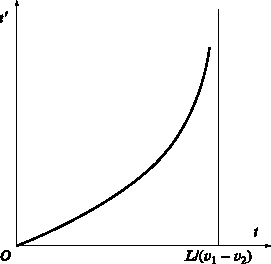
\includegraphics{figure/fig01.03}
  \caption{芝诺时的定义}\label{fig:01.03}
  %\vspace{-1.2em}
\end{wrapfigure}
\noindent 间的度量达到无限之后,还是可以有时间的;反之,一种时
间的度量达到无限,从其他的度量看,可能是有限的。

芝诺佯谬还启发我们提出一个更深入的问题,即所谓普通钟
或日常钟是否也具有芝诺钟那种局限性?当日常钟$t$的读数达到
无限之后,是否也还有时间?是否有$t$也无法度量的现象,即在
$t\rightarrow\infty$之外的现象?现代物理学的研究,对这些
问题的回答都是肯定的。

\section[长度]{\makebox[5em][s]{长度}}\label{sec:01.03}

长度是空间的一个基本性质。

对长度的测量,在日常的范围中,是用各种各样的尺,如米
尺、千分尺、螺旋测微计等等。对于不能用尺直接加以测量的小
尺度,可以求助于光学方法。在精密机床上常有光学测量装置;
测定胰岛索中原子的位置,是用X衍射方法。对于大的尺度,
也不能直接用尺去测量,也要求助于光。测量月亮与地球的距离
可以用激光测距的方法;测量一些不太远的恒星,可以用三角学
方法,利用恒星发出的光。至于银河系之外的遥远天体的距离,
同样是用它们发光的一些特征来测定的。

最近,长度的单位和标准,也用光来规定了。

长度的位单是米。1960年以前,用铂铱米尺作为标准尺,规
定米的大小。1960年以后,改用光的波长作为标准。在第十一届
国际计量大会上,正式通过的“米”的定义是l米等于$^{86}$Kr原子
\clearpage\noindent
的$2\rm{p}_{10}$和$5\rm{d}_5$
能级之间跃迁时所对应的辐射在真空中的波长$\lambda$的1,650,763.73倍,即
\begin{equation*}
 1 \text{米} = 1,650,763.73 \, \lambda
\end{equation*}

1983年10月召开的第十七届国际计量大会上已正式通过了
\begin{table}[!h]
 \centering
 \caption{一些典型物理现象的空间尺度}
 \label{tab:01.03}
 \begin{tabular*}{\linewidth}{>{\centering}m{\linewidth}c}
 \toprule
 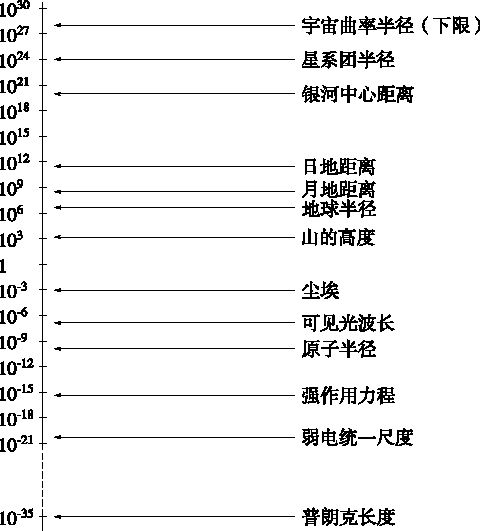
\includegraphics[width=0.8\linewidth]{figure/tab01.03} & \\
 \bottomrule
 \end{tabular*}
\end{table}
\clearpage

\noindent 新的米的定义,即用光速值来定义“米”,以代替1960年的规定。
新的米的定义是,米是光在真空中在$ 1/299,792,458 $秒的时间间隔
内所传播的路程长度。按这种新的定义,光速$ c $是一固定的常数,即
\begin{equation*}
 c = 299,792,458 \, \text{米/秒}
\end{equation*}

表\ref{tab:01.03}中列举了一些典型现象的空间尺度。目前,物理学中涉
及的最太长度是$10^{28}$米,它是宇宙曲率半径的下限;已达到的最
小长度为$10^{-20}$米,它是弱电统一的特征尺度。普朗克长度约为
$10^{-35}$米,被认为是最小的长度,意思是说,在比普朗克长度更小
的范围内,长度的概念可能就不再适用了。

\section[参考系]{参~~考~~系}\label{sec:01.04}

牛顿力学所研究的对象是物体的机械运动。从我们日常见到
的车行马跑,及至大到月亮、太阳等星体的运行,小到分子、原子、
粒子的一些飞行,都是属于这一类运动。这类运动的共同特点,
就是物体在空间的位置时刻在变化着。当然,静止的状态、平衡
的状态也是力学的内容之一。

牛顿意义下的运动学,就是研究如何描写物体位置的变化。

研究问题总是从简单的情况入手。我们首先讨论一种被称为
质点的物体,即大小为零的物体。我们知道,任何具体的物体总
是有一定大小的,没有任何一个物体与质点完全等价。但是,对
于某些特定的运动来说,可以足够准确地把物体看作一个质点。
譬如,在讨论地球绕太阳的公转时,由于地球的半径(约$ 6,400 $公
里)比地球与太阳的距离(约$ 149,504,000 $公里)小得多,把地球作
为质点是相当好的近似,或者说,在此情况下,将地球作为质点
处理,是一个足够准确的模型。显然,这种模型是有一定适用限
度的。当讨论到地表问题时,再把地球看作质点就大谬不然了。

质点是一个物理对象。对于一个物理对象,用什么数学语言
来描写,这并不是一件很自然的事情,我们知道,任何一种数学
只是一种逻辑体系,一种逻辑体系能不能正确地描写我们的物理
对象,是要认真研究的。物理上,就是要寻找那种能正确地描写
物理对象的数学。在牛顿力学中,质点的空间几何性质,相当于
欧几里德几何上的点。在解析几何中,点的位置是由它的坐标值
来确定的。质点的位置也可以用这种坐标方法来给定。利用坐标
方法,首先要给出坐标系,坐标值总是相对于一定的坐标系而言
的。在数学上,坐标系的选取是完全任意的,但在物理上,我们
要对描写运动的各种物理量进行实际测量,坐标必须固定在一定
\begin{wrapfigure}[11]{l}{13em}
  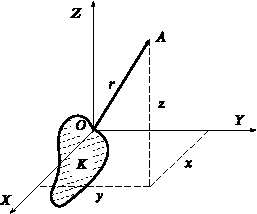
\includegraphics{figure/fig01.04}
  \caption{参考系$K$及参考坐标系$OXYZ$}
  \label{fig:01.04}
\end{wrapfigure}
的物体上。例如,如果选取物体$K$上的某点$O$为坐标原点,并选
定$x$,$y$,$z$三个轴,质点$A$的位置即由$x$,$y$,$z$所确定(图\ref{fig:01.04})。
这时,我们称所选取的物体$K$为参考系,而称坐标系$OXYZ$为参
考坐标系。

除了坐标方法外,也可以利用矢量方法来描写质点A的位
置。我们定义质点$A$的位置矢量$\vec{r}$的大小为$OA$的长度,而方向从
$O$指向$A$。用这个矢量就完全确定了质点$A$的位置。在图1.4的坐
标系中,位置矢量$r$的分量就是坐标$x$,$y$,$z$,或写为
\begin{equation}\label{eqn:01.04.01}
  \vec{r}=x\vec{i}+y\vec{j}+z\vec{k}
\end{equation}
其中$\vec{i}$,$\vec{j}$,$\vec{k}$分别为$X$,$Y$,$Z$轴上的单位矢量,上述两种描述
质点$A$的位置的方法,是完全等价的。

参考系的选择是任意的,可以不用参考系$K$,而用另外一
\begin{wrapfigure}[9]{r}{13em}
  
\includegraphics{figure/fig01.05}
  \caption{\ziju{-0.02}从不同参考系观察同一运动}
  \label{fig:01.05}
\end{wrapfigure}
个参考系$K'$,譬如,用运动着的车辆来描述质点$A$的位置。由图\ref{fig:01.05}
看到,对干参考系$K$,质点$A$的位置由矢量$\vec{r}$描写,而对于参考
系$K'$,由$\vec{r'}$描写。可见,对于同一个质点的位置,用不同参考系
来描写时,具有不同的位置矢量。就这一点,我们可以说,位
置是具有相对性的物理量。涉及物理量的相对性与绝对性的问题,
以后我们还要专门论述。
\section[轨迹]{\makebox[5em][s]{轨迹}}\label{sec:01.05}

谁都看到过,当喷气式飞机在飞行的时候,它的尾部泄出的
白烟在天空中构成形状美丽的各样曲线。这些曲线反映了飞机所
行经的路程。质点在运动中所经过的各点在空间连成一条曲线,
这条曲线我们称之为轨迹。

\begin{figure}[!h]
  \hspace{3em}
  \subfigure[\null]{
    \label{fig:01.06a}
    
\includegraphics{figure/fig01.06a}
  }
  \hspace{3em}
  \subfigure[\null]{
    \label{fig:01.06b}
    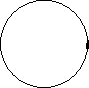
\includegraphics{figure/fig01.06b}
  }

  \hspace{3.7em}
  \subfigure[\null]{
    \label{fig:01.06c}
    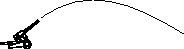
\includegraphics{figure/fig01.06c}
  }
  \hspace{1.3em}
  \subfigure[\null]{
    \label{fig:01.06d}
    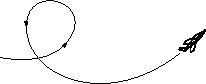
\includegraphics{figure/fig01.06d}
  }
  \caption{各种运动的轨迹}
  \label{fig:01.06}
\end{figure}

\clearpage

从图\ref{fig:01.06}看到,各种运动的轨迹形状是不同的;\subref{fig:01.06a}图是直线,
\subref{fig:01.06b}图是圆周,\subref{fig:01.06c}图是抛物线,\subref{fig:01.06d}图是一般曲线。依照轨迹形状
的不同,可以把运动分为直线运动和曲线运动两大类。

如何描写轨迹呢?可利用曲线方程来描写。譬如,曲线方程 \begin{equation*}
  \begin{aligned}
     & x^2+y^2=r^2 \\
     & z=0
  \end{aligned}
\end{equation*}
就描写了在$z=0$平面上半径为$r$的圆周运动的轨迹。一般曲线方
程可以表示成
\begin{equation*}
  \begin{aligned}
    f_1\left(x,y,z\right)=0 \\
    f_2\left(x,y,z\right)=0
  \end{aligned}
\end{equation*}

在历史上很长一个时期内,人们只注重轨迹形状的研究,例
如行星走圆形,落体走直线。我们知道,质点运动是位置的变化,
它涉及空间和时间两方面。轨迹形状只反映了运动的空间方面的
性质,它对于研究运动还是不够的,因为轨迹还没有把质点运动
的情况全部表述出来,特别是没有表述它的动态性质。百米赛跑
时,所有运动员的轨迹都是直线,但他们各自的运动情况并不全
同,否则就分不出名次了。我们不仅应该知道轨迹,而且还应知
道质点经过轨迹上各点的时刻。运动是在时间、空间里的现象,
关键是把时间描写和空间描写联系起来。直到牛顿之前不久,才
特别强调了这一点。

下面,我们举两个直线运动的例子。

对于在平直铁轨上稳定运动的列车上的某一点,所测得的各
时刻的位置列于表\ref{tab:01.04}中,其中位置坐标$x$是以铁轨为参考系的(图\ref{fig:01.07})。
\begin{table}[h]
  \caption{}
  \label{tab:01.04}
  \centering
  \zihao{-5}
  \begin{tblr}{c*{6}{|X[c]}}
    \toprule
    时\hspace{2em}间(秒) & 0 & 1  & 2  & 3  & 4  & 5  \\
    \midrule
    位置坐标(米)           & 0 & 17 & 34 & 51 & 68 & 85 \\
    \bottomrule
  \end{tblr}
\end{table}

\begin{figure}[!h]
  \centering
  
\includegraphics{figure/fig01.07}
  \caption{列车的运动}
  \label{fig:01.07}
\end{figure}

对于从地面上某一高度自由落下的质点(称为自由落体),轨
迹也是一条直线。如果我们取如图\ref{fig:01.08}所示的坐标系,则所测得的
质点在各时刻的位置列在表\ref{tab:01.05}中。
\begin{table}[!h]
  \caption{}
  \label{tab:01.05}
  \zihao{-5}
  \centering
  \begin{tblr}{c*{5}{|X[c]}}
    \toprule
    时\hspace{2em}间(秒) & 0 & 1   & 2    & 3    & 4    \\
    \midrule
    位置坐标(米)           & 0 & 4.9 & 19.6 & 44.1 & 78.4 \\
    \bottomrule
  \end{tblr}
\end{table}

用数学的语言说,表\ref{tab:01.04}~和表\ref{tab:01.05}~是给出了质点的位置坐标与
时间之间的函数关系,这个函数关系$x\left(t\right)$,称之为轨迹函数,或
\begin{wrapfigure}[14]{l}{8em}
  \centering
  
\includegraphics{figure/fig01.08}
  \\ ~ \\
  \caption{落体的运动}
  \label{fig:01.08}
\end{wrapfigure}
运动方程式、运动解。

为了便于进行计算,我们常希望能把轨迹
函数$x\left(t\right)$写成简单的分析表达式。对于表\ref{tab:01.04}~
的$x\left(t\right)$,可以写成
\begin{equation}\label{eqn:01.05.01}
  x=17t
\end{equation}
对于表\ref{tab:01.05}~的运动,可以写成$x=4.9t^2$。

对于曲线运动,轨迹函数就是位置矢量$\vec{r}$作为时间
$t$的函数,亦即$\vec{r}\left(t\right)$。随着$t$的变化,位置矢量$\vec{r}$的
端点在空间所划出的曲线,就是质点运动的轨迹(图\ref{fig:01.09})。也可
以用质点的三个坐标的函数$x\left(t\right)$,$y\left(t\right)$及$z\left(t\right)$来描写运
动,它们与$r\left(t\right)$的关系是
\clearpage
\begin{equation}\label{eqn:01.05.02}
  \vec{r}\left(t\right)=x\left(t\right)\vec{i}+y\left(t\right)\vec{j}+z\left(t\right)\vec{k}
\end{equation}

\begin{wrapfigure}[7]{r}{11em}
  \centering
  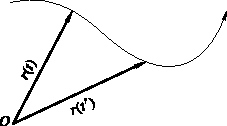
\includegraphics{figure/fig01.09}
  \caption{曲线运动}
  \label{fig:01.09}
\end{wrapfigure}
轨迹也具有相对性。譬如对于从地面上某一高度自由下落的质点,以
地面为参考系,看到轨迹是一条直线;而相对于沿平直铁轨稳定运行的
列车来说,轨迹则是一条抛物线。同一个物体的运动,在不同的参考系中
看到的轨迹形状不一定相同。

另一方面,对于时间,也必须选取一定的标准,即选取时间
原点,才能进行测量。而时间原点的选取,也有任意性,不同的
选取法,使轨迹函数的形式也有些差别。

因此,参考系的概念要作些扩充。选取一个参考系应包括:
给定放置在某物体上的坐标系,作为测量空间的标准;以及给定
一个钟,作为测量时间的标准。

\section{速度的瞬时性}\label{sec:01.06}

机械运动的现象,给了我们对“快”、“慢”的经验认识。
火车比轮船快,飞机比火车快,而火箭更比飞机快等等。反映质
点运动快慢的物理量就是速度,或者确切地说,是速度的数值大小。

先以直线运动为例,当时刻$ t_1 $时,质点$ A $的位置坐标为$ x\left(t_1\right) $,
当$ t_2 $时,它的坐标为$ x\left(t_2\right) $,我们就用下式来定义质点$ A $在$ t_1 $到
$ t_2 $时间间隔内的平均速度:
\begin{equation}
  \langle v\rangle_{t_{1} \rightarrow t_{2}}=\frac{x\left(t_{2}\right)-x\left(t_{1}\right)}{t_{2}-t_{1}} \label{eqn:01.06.01}
\end{equation}
符号$\langle ~ \rangle$表示所讨论的量的平均值。$\langle v\rangle_{t_{1} \rightarrow t_{2}}$的数值表示质点
在时
\clearpage
\noindent 间间隔$t_{1} \rightarrow t_{2}$中每单位时同平均走过的距离,它的单位是
米/秒。利用表\ref{tab:01.04}所给出的运动进行计算,就有:在第1秒末到
第2秒末间隔中,
\begin{equation*}
  \langle v\rangle_{1 \rightarrow 2}=\frac{34-17}{2-1}=17\,\text{米/秒}
\end{equation*}
在第3秒末到第5秒末间隔中,
\begin{equation*}
  \langle v\rangle_{3 \rightarrow 5}=\frac{85-51}{5-3}=17\,\text{米/秒}
\end{equation*}
选两个时间间隔中平均速度是一样的。事实上,如果利用分析表
达式\eqref{eqn:01.05.01}来计算,就会发现对任何时间间隔,运动的平均速度
都是17米/秒。这种对于任何时间间隔平均速度总不变的运动,称
为匀速直线运动。

由表\ref{tab:01.05}或$x=4.9t^2$所示的自由落体运动,情况就不同了:
在第1秒末到第3秒束的问隔中,
\begin{equation*}
  \langle v\rangle_{1 \rightarrow 3}=\frac{44.1-4.9}{3-1}=19.6\,\text{米/秒}
\end{equation*}
在第1秒末到第2秒末的间隔中,
\begin{equation*}
  \langle v\rangle_{1 \rightarrow 2}=\frac{19.6-4.9}{2-1}=14.7\,\text{米/秒}
\end{equation*}
在第2秒末到第3秒末的间隔中,
\begin{equation*}
  \langle v\rangle_{2 \rightarrow 3}=\frac{44.1-19.6}{3-2}=25.4\,\text{米/秒}
\end{equation*}
对于不同的时间间隔。自由落体的平均速度不相同。这种运动称
为变速运动。从上面所给出的三个平均速度可知,自由落体在第
1秒末到第3秒末的两秒钟时间间隔中并非匀速,它在前一秒钟
(即第1秒末到第2秒末)平均速度较小,在后一秒钟(即第2秒末
到第3秒末)平均速度较大。从这一点上可以充分反映出平均速度
往往不足以描写变速运动的细致情况。这是平均速度概
念的弱点。求平均速度的时间间隔取得越大,它对快慢的描述就越粗略;
反之,时间间隔越小,对快慢的描述也就越精确。在上例中,虽
然取1秒的时间间隔,比取2秒的时间间隔要好一些,但是在一
秒钟的时间间隔内,自由落体仍然不是匀速的。这种情况迫使我
们把计算平均速度的时间间隔取得尽可能地小。

为了便于进一步讨论,我们将式\ref{eqn:01.06.01}中的
$t_2$表示成$t_2=t_1+\Delta t$,这个$\Delta t$就是求平均速
度所选用的时间间隔。现在来求从第1秒末到第$1+\Delta t$秒末
的间隔中,自由落体的平均速度。利用$x=4.9t^2$得到
\begin{equation*}
  \begin{aligned}
    \langle v\rangle_{1 \rightarrow 1+\Delta t} & =\frac{x\left(1+\Delta t\right)-x\left(1\right)}{1+\Delta t-1}           \\
                                                & =\frac{4.9 \times\left(1+\Delta t\right)^{2}-4.9 \times 1^{2}}{\Delta t} \\
                                                & =\left(9.8+4.9 \Delta t\right) \text { 米/秒 }
  \end{aligned}
\end{equation*}
此式再次表明,从第1秒末开始取不同的时间间隔$\Delta t$,所得的平
均速度是不相同的。既然$\Delta t$越小描述得越精确,我们取
$\Delta t$为无限小,或者相当于$\Delta t \rightarrow 0$的
极限情况,这时平均速度变成为:
\begin{equation*}
  \lim _{\Delta t \rightarrow 0}\left(9.8+4.9 \Delta t\right)=9.8 \text { 米/秒 }
\end{equation*}
这个9.8米/秒的物理意义是自由落体在第1秒末的一个无限小时
间间隔中的平均速度,我们称这个值为自由落体在第1秒末的瞬
时速度。瞬时速度与平均速度这两个概念的重要区别在于:平均
速度总是与一段有限的时间间隔相联系,它是描述一段运动过程
的物理量;相反,瞬时速度与一个时刻相联系,它是描述运动的
瞬时性质的物理量。有了瞬时速度这个概念,使我们对运动的认
识大为深化。

用类似的手续不难求出自由落体运动在任何时刻t的瞬时速
度$v\left(t\right)$,只要将上述的1及$1+\Delta t$分别代之以$t$及$t+\Delta t$,并取
于$\Delta t \rightarrow 0$的极限值就可以了。故有

\begin{equation}\label{eqn:01.06.02}
  \begin{aligned}
    v\left(t\right) & =\lim _{\Delta t \rightarrow 0} \frac{x\left(t+\Delta t\right)-x\left(t\right)}{\Delta t}               \\
                    & =\lim _{\Delta t \rightarrow 0} \frac{4.9 \times\left(t+\Delta t\right)^{2}-4.9 \times t^{2}}{\Delta t} \\
                    & =\lim _{\Delta t \rightarrow 0}\left(9.8 t+4.9 \Delta t\right)                                          \\
                    & =9.8 t
  \end{aligned}
\end{equation}
此式给出了自由落体在每个时刻的瞬时速度。根据这个结果,我
们再强调一遍,自由落体的运动快慢是时刻变化着的。你用平均
速度来描写它,无论$\Delta t$取如何小的有限值,即使小到$\Delta t$=0.001
秒,依然不够精确,因为在这0.001秒中质点依然不是匀速运动
的。只有$\Delta t$趋于无限小,给出了每个时刻$t$的瞬时速度,了解了
质点运动在每一瞬时的快慢,才算最精确地反映了质点运动的快
慢。

对于任何直线运动,它的瞬时速度都可以用类似方式来确
定:
\begin{equation*}
  v\left(t\right)=\lim _{\Delta t \rightarrow 0} \frac{x\left(t+\Delta t\right)-x\left(t\right)}{\Delta t}
\end{equation*}
根据微积分学的知识,该极限就是轨迹函数$x\left(t\right)$对时间t的一阶
导数。即
\begin{equation}
  \begin{aligned}
    v\left(t\right) & =\lim _{\Delta t \rightarrow 0} \frac{x\left(t+\Delta t\right)-x\left(t\right)}{\Delta t}            \\
                    & =\lim _{\Delta t \rightarrow 0} \frac{\Delta x}{\Delta t}=\frac{\dif x}{\dif t} \label{eqn:01.06.03}
  \end{aligned}
\end{equation}
其中,$\Delta x=x\left(t+\Delta t\right)-x\left(t\right)$,是在$t\rightarrow t+\Delta t$时间间隔中质点位置
坐标的增量。以后我们提到的速度,一般都指瞬时速度。

我们看到,瞬时速度是利用数学上的微分概念来描写的。其
实,在历史上,正是由于牛顿在处理这类基本力学问题时需要一
种适当的数学工具,从而促使他创建了微积分学。这不仅使物理
概念得以准确地表述,而且也大大丰富了数学本身。这是牛顿的
巨大功绩之一。\ziju{-0.02}由此,我们再次看到,一个物理对象,用什么数学
语言描写并不是一件自然的事情,而是物理研究的一个核心课题。\ziju{0}

\begin{wrapfigure}[10]{r}{13em}
  \centering
  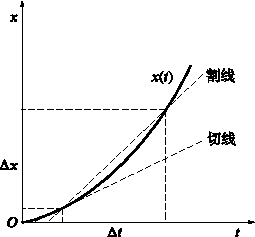
\includegraphics{figure/fig01.10}
  \caption{直线运动的$x \mathdash t$图}
  \label{fig:01.10}
\end{wrapfigure}
当质点作直线运动时,我们
可以设法求出它的位置时间曲线
(图\ref{fig:01.10})。从图中可以看出,平
均速度在数值上等于各段割线的
斜率,瞬时速度在数值上等于各
点的切线的斜率。所以在求出位
置时间曲线后,就可以从$x\left(t\right)$曲
线上求出各点的速度。

从平均速度的定义(\ref{eqn:01.06.01})式可以知道,$\langle v\rangle$可以有正值,
也可以有负值。当$x\left(t+\Delta t\right)<x\left(t\right)$时,$\langle v\rangle$为负。这种情况相当
于质点在$t$到$t+\Delta t$间隔中,总的说来是向负$x$方向运动的。所
以,$\langle v\rangle$的正负恰恰反映了运动的方向。通常称平均速度的绝对
值$|\langle v\rangle|$为平均速率。类似地,瞬时速度的绝对值$|\vec{v}\left(t\right)|$被称为
速率,而瞬时速度的正负,就表示质点在时刻$t$的运动方向。速
度$\vec{v}$不仅描述了运动的快慢,而且描述了运动方向。

\section{曲线运动的速度}\label{sec:01.07}

\ziju{-0.02}我们现在来推广上节关于直线运动的速度的概念。按图1.11,
质点作曲线运动,在时刻$t_1$,质点位置矢量为$\vec{r}\left(t_1\right)$,在时刻$t_2$,
位置矢量为$\vec{r}\left(t_2\right)$,则定义在$t_1$到$t_1$间隔中质点A的平均速度为\ziju{0}
\begin{equation}\label{eqn:01.07.01}
  \langle \vec{v} \rangle_{t_1\rightarrow t_2}=\frac{\vec{r}\left(t_2\right)-\vec{r}\left(t_1\right)}{t_2-t_1}=\frac{\Delta \vec{r}}{\Delta t}
\end{equation}

\noindent 将其与式\eqref{eqn:01.06.01}~对比可见。只是将其中的$x\left(t\right)$换成了相应的
$\vec{r}\left(t\right)$。在\eqref{eqn:01.07.01}~中,$\Delta t=t_2-t_1$,$\Delta \vec{r}=\vec{r}\left(t_2\right)-\vec{r}\left(t_1\right)$,
后者是$t_1$到$t_2$间隔
\begin{wrapfigure}[8]{r}{12em}
  \centering
  \small
  
\includegraphics{figure/fig01.11}
  \caption{曲线运动的速度}
  \label{fig:01.11}
\end{wrapfigure}
中质点位置矢量的改变量,称为位移矢量。这个平均速度的定义表明,平均速度是矢量。根据矢量运算
规则,式\eqref{eqn:01.07.01}~所定义的$\langle \vec{v}\rangle t_1-t_2$是在l到2的方向(图\ref{fig:01.11})。
另一方面,由图\ref{fig:01.11}~很清楚知道,在$t_1$到$t_2$时间内质点$A$的运
动方向并非总是沿着l到2的方向的,而是先从1向3方向运动,
然后从3向2方向运动,这些运动方向并不平行于1到2的方向。
所以平均速度所指的方向,只是质点$A$真实运动方向的平均。
也就是说,平均速度不但对于运动快慢的描写是粗
略的,而且对于运动方向的描写也是粗略的。

对式\eqref{eqn:01.07.01}~取$\Delta t \rightarrow 0$的极限,就得到瞬
时速度的定义。
\begin{equation}\label{eqn:01.07.02}
  \begin{aligned}
    \vec{v}\left(t\right) & =\lim _{\Delta t \rightarrow 0} \frac{\vec{r}\left(t+\Delta t\right)-\vec{r}\left(t\right)}{\Delta t} \\
                          & =\lim _{\Delta t \rightarrow 0} \frac{\Delta \vec{r}}{\Delta t} =\frac{\dif\vec{r}}{\dif t}
  \end{aligned}
\end{equation}
它是直线运动情况的式\eqref{eqn:01.06.03}的推广。如果利用式\eqref{eqn:01.04.01},则
有
\begin{equation}\label{eqn:01.07.03}
  \vec{v}\left(t\right)=\frac{\dif x\left(t\right)}{\dif t} \vec{i}+\frac{\dif y\left(t\right)}{\dif t} \vec{j}+\frac{\dif z\left(t\right)}{\dif t} \vec{k}
\end{equation}
所以三个坐标函数$x\left(t\right)$,$y\left(t\right)$,$z\left(t\right)$对时间t的导数分别是速度矢
量在三个坐标轴方向的分量:
\begin{equation}\label{eqn:01.07.04}
  v_{x}=\frac{\dif x\left(t\right)}{\dif t}, ~ v_{y}=\frac{\dif y\left(t\right)}{\dif t}, ~ v_{z}=\frac{\dif z\left(t\right)}{\dif t}
\end{equation}
\clearpage
\begin{wrapfigure}[7]{r}{13em}
  \centering
  \small
  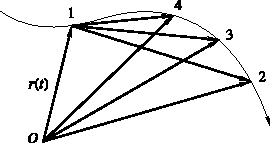
\includegraphics{figure/fig01.12}
  \caption{曲线运动的瞬时速度}
  \label{fig:01.12}
\end{wrapfigure}
由图\ref{fig:01.12},当$\Delta t$减小时,矢量$\vec{r}\left(t+\Delta t\right)$
逐渐向$\vec{r}\left(t\right)$靠拢,矢量$\Delta \vec{r}$相继从1,2变到1,3,
变到1,4……,在$\Delta t \rightarrow 0$的极限情况下,$\Delta \vec{r}$
的方向趋于轨迹曲线在点1的切线方向。这样,我们就得到一个
结论:瞬时速度$\vec{v}\left(t\right)$的方
向,就是轨迹曲线在相应点的切线方向。瞬时速度的大小$v$,按
定义\eqref{eqn:01.07.02}应为
\setlength{\mathindent}{15em}
\begin{equation*}
  \begin{aligned}
    v\equiv |\vec{v}| & =\left|\lim _{\Delta t \rightarrow 0} \frac{\Delta \vec{r}\left(t\right)}{\Delta t}\right| \\
                      & =\lim _{\Delta t \rightarrow 0} \frac{|\Delta \vec{r}|}{\Delta t}
  \end{aligned}
\end{equation*}

\setlength{\mathindent}{6em}
\begin{wrapfigure}[4]{l}{10em}
  \vspace{-6em}
  \centering
  \small
  
\includegraphics{figure/fig01.13}
  \caption{用路程长度$s\left(t\right)$来描写运动}
  \label{fig:01.13}
\end{wrapfigure}
\noindent 我们可以引入路程长度概念来描写运动。如图\ref{fig:01.13},若当$t=0$时,
质点在轨迹上的$P$处。则可定义函数$s\left(t\right)$,它表示质点到$t$时刻所
走过的路程的长度。显然,$\Delta s=s\left(t+\Delta t\right)-s\left(t\right)$表示
在$t$到$t+\Delta t$中质点所走过的路程的长度。一般$\Delta s$和
$|\Delta \vec{r}|$并不相等,但在$\Delta t \rightarrow 0$的极限情况
下,二者是一样的,故速度大小也可表示为
\begin{equation}\label{eqn:01.07.05}
  v=\lim_{\Delta t \rightarrow 0}\frac{\Delta s}{\Delta t}=\frac{\dif s}{\dif t}
\end{equation}


\section[加速度]{加\hspace{1em}速\hspace{1em}度}\label{sec:01.08}

为了描写速度的变化,我们再引入一个物理量,即所谓加速
度。对于直线运动,若当$t$时刻,质点速度为$v\left(t\right)$,当$t+\Delta t$时
刻,为$v\left(t+\Delta t\right)$,则我们定义从$t$到$t+\Delta t$间隔中质点的平均加
速度为\\~\vspace{-2em}
\begin{equation}\label{eqn:01.08.01}
 \langle a\rangle_{t\rightarrow t+\Delta t} = \frac{v\left(t+\Delta t\right)-v\left(t\right)}{\Delta t}
\end{equation}
它的定义是质点在单位时间中速度的平均变化,单位是$\text{米/秒}^2$。

利用式\eqref{eqn:01.06.02},可以计算自由落体在$t$到$t+\Delta t$间隔中的平
均加速度:\vspace{-1em}
\begin{equation*}
 \begin{aligned}
 \langle a\rangle_{t\rightarrow t+\Delta t} & = \frac{9.8\left(t+\Delta t\right)-9.8t}{\Delta t} \\
 & = 9.8\text{米/秒}^2
 \end{aligned}
\end{equation*}
这个结果中不含$t$和$\Delta t$,也就是说,对任何一段时间间隔,自由落
体的平均加速度都是一样的。这种加速度不随时间变化的运动,
称为匀加速运动。自由落体运动是一个典型的匀加速运动。无论
用何种材料作成的物体,它的自由落体加速度总等于9.8~$\text{米/秒}^2$。
称此加速度为重力加速度,用$g$表示。

精确测量表明,在地球各处,重力加速度$g$并不都一样,一
\begin{table}[h]
 \caption{地球上不同地点的$g$值}
 \label{tab:01.06}
 \centering
 \zihao{-5}
 \begin{tblr}{colsep=2em,colspec={l|l|Z}}
 \toprule
 地\hspace{7em}点 & 纬\hspace{1.5em}度 & $g$~{{{(米/秒\textsuperscript{2}) }}} \\
 \midrule
 北\quad 极 & 北纬 \ang{90} & 9.83245 \\
 戈拉雅克(格陵兰) & 北纬 \ang{70} & 9.8253 \\
 雷克雅未克(冰岛) & 北纬 \ang{64} & 9.8227 \\
 列宁格勒 & 北纬 \ang{60} & 9.8193 \\
 巴\quad 黎 & 北纬 \ang{49} & 9.8094 \\
 北\quad 京 & 北纬 \ang{40} & 9.8012 \\
 汉\quad 口 & 北纬 \ang{30} & 9.7936 \\
 广\quad 州 & 北纬 \ang{23} & 9.7883 \\
 蒙罗维亚(利比里亚) & 北纬 \ang{6} & 9.7816 \\
 雅加达 & 南纬 \ang{6} & 9.7813 \\
 墨尔本 & 南纬 \ang{38} & 9.7999 \\
 \bottomrule
 \end{tblr}
\vspace{-0.8em}
\end{table}
\clearpage
\noindent 般说来,在低纬度处$g$值较小;在高纬度处,$g$值较大(表\ref{tab:01.06})。

类似于平均速度不足以细致地描写非匀速运动一样,平均加
速度也不足以细致地描写非匀加速运动。对于非匀加速运动,必
须引入瞬时加速度来描述它的速度变化。加速度也是一个描述运
动的瞬时性质的物理量。瞬时加速度定义为:
\begin{equation*}
 \begin{aligned}
 a\left(t\right) & =\lim _{\Delta t \rightarrow 0} \frac{v\left(t+\Delta t\right)-v\left(t\right)}{\Delta t} \\
 & =\frac{\dif v\left(t\right)}{\dif t}=\frac{\dif^2 x\left(t\right)}{\dif t^2}
 \end{aligned}
\end{equation*}
它的意义是质点在时刻t的无限小时间间隔中的平均加速度。以
后我们谈到加速度,一般都是指瞬时加速度。

对于一般的曲线运动,可以给出相应的平均加速度及瞬时加
速度为:
\begin{equation}\label{eqn:01.08.02}
 \langle \vec{a} \rangle_{t \rightarrow t+\Delta t} = \frac{\vec{v}\left(t+\Delta t\right)-\vec{v}\left(t\right)}{\Delta t}
\end{equation}
\begin{equation}\label{eqn:01.08.03}
 \begin{aligned}
 \vec{a}\left(t\right) & =\lim _{\Delta t \rightarrow 0} \frac{\vec{v}\left(t+\Delta t\right)-\vec{v}\left(t\right)}{\Delta t} \\
 & =\lim_{\Delta t \rightarrow 0}\frac{\Delta \vec{v}}{\Delta t} \\
 & =\frac{\dif\vec{v}\left(t\right)}{\dif t}=\frac{\dif^2 \vec{r}\left(t\right)}{\dif t^2}
 \end{aligned}
\end{equation}
在曲线运动情况下,速度方向是变化的。$v\left(t\right)$,$v\left(t+\Delta t\right)$及$\Delta v$,
\begin{wrapfigure}[6]{r}{13em}
 %\vspace{-6em}
 \centering
 \small
 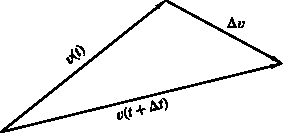
\includegraphics{figure/fig01.14}
 \caption{加速度的计算}
 \label{fig:01.14}
\end{wrapfigure}
一般如图\ref{fig:01.14}~所示。由于$a$平行于$\Delta v$,所以平均加速度的方向一
般与速度方向并不相同。瞬时加速度也类似。当加速度方向平行
于速度时,表示速度方向没有变化,但速率增加。当二者反平行
\clearpage\noindent
时,表示速度方向不变,而速率减少。当加速度既不平行也不反
平行于速度时,表示速度方向也在变化。

利用式\eqref{eqn:01.07.03},加速度矢量的分量可以表示为:
\begin{equation}\label{eqn:01.08.04}
 \vec{a}=\frac{\dif^2x\left(t\right)}{\dif t^2}\vec{i}+\frac{\dif^2y\left(t\right)}{\dif t^2}\vec{j}+\frac{\dif^2z\left(t\right)}{\dif t^2}\vec{k}
\end{equation}
加速度的三个坐标分量为:
\setlength{\mathindent}{4em}
\begin{equation}\label{eqn:01.08.05}
 a_x(t)=\frac{\dif^2x\left(t\right)}{\dif t^2},~ a_y(t)=\frac{\dif^2y\left(t\right)}{\dif t^2},~
 a_z(t)=\frac{\dif^2z\left(t\right)}{\dif t^2}
\end{equation}
\setlength{\mathindent}{6em}

$\vec{r}$,$\vec{v}$,$\vec{a}$是描写运动的物理量。我们希望用数目比较少的物
理量来描写运动。什么叫比较少?意思是这些物理量之间应是相
互独立的。所谓相互独立。是说其中任一个量不能由其他的量加
以确定。用$\vec{r}$,$\vec{v}$及$\vec{a}$三个量来描写运动是必要的,因为它们是相互
独立的。例如,在某一时刻,知道了质点的位置$\vec{r}$,并不能知道
它的速度$\vec{v}$,知道了$\vec{v}$,也并不能知道$\vec{a}$,反之亦然。人们认识到
这一点,也并不容易。在伽利略之前,并没有加速度概念。当时,
没有人认识到加速度与速度是相互独立的,所以没有认识到需要
用加速度来描写运动。

我们已讨论了位置矢量、速度和加建度。从运动学本身来考
虑,没有足够的理由说明,为什么我们应当到此为止,而不去讨
论加加速度、加加加速度……。当然,我们可以定义并计算加加
速度,即加速度的变化率,但一般说这并不代表任何具有基本物
理价值的东西。其中的原因在动力学,学过动力学后,我们将看
到,对力学的讨论几乎全部是基于位置矢量,速度和加速度这三
个量。

下面我们介绍运动的独立性这一重要概念。由式\eqref{eqn:01.05.02}、
\eqref{eqn:01.07.03}、\eqref{eqn:01.08.05}可以看到,描写一个复杂的曲线运动时,$X$方
向的坐标、速度、加速度与其他方向的坐标,速度、加速度无关。
$Y$方向和$Z$方向也有这种性质,即三个方向相互无关,这种性质被
称为运动的独立性。因此,一个复杂的曲线运动,可看成在$X$,$Y$,
$Z$三个方向上的直线运动,这三个运动同时进行,我们可以对每
一个运动进行单独的分析,好象另外两个自由度上的运动是根本
不存在一样,这样就使问题变得简单。

\example 已知一个质点作直线运动。观察到它的位置与时间
的变化如表\ref{tab:01.07}所示。用这些数据求出各时间间隔的平均速度$v$及
平均加速度$a$,并写出运动方程式。
\begin{table}[!h]
 \caption{}
 \label{tab:01.07}
 \centering
 \zihao{-5}
 \begin{tblr}{l*{9}{|X}}
 \toprule
 时~~~~间(秒) & 0 & 1 & 2 & 3 & 4 & 5 & 6 & 7 & 8 \\
 \midrule
 {与参考点的距离 (米)} & 3 & 4 & 9 & 18 & 31 & 48 & 69 & 94 & 123 \\
 \bottomrule
 \end{tblr}
\vspace{-0.8em}
\end{table}

\solution 因为时间间隔都是1秒,即$\Delta t=1$秒。所以从数值上有
\begin{align*}
 v & =\frac{\Delta s}{\Delta t}=\Delta s \\
 a & =\frac{\left(v_2-v_1\right)}{\Delta t}=v_2-v_1=\left(\Delta s_2\right)-\left(\Delta s_1\right)
\end{align*}
将结果列于表\ref{tab:01.08}中。
\begin{table}[!h]
 \caption{}
 \label{tab:01.08}
 \centering \zihao{-5}
 \setlength{\tabcolsep}{0em}
 \begin{tblr}{colsep=0pt,colspec={l*{17}{|X[c]}}}
 \toprule
 时~~~~间(秒) & 0 & & 1 & & 2 & & 3 & & 4 & & 5 & & 6 & & 7 & & 8 \\
 \midrule
 {与参考点的距离\\\qquad$s$~~(米)} & 3 & & 4 & & 9 & & 18 & & 31 & & 48 & & 69 & & 94 & & 123 \\
 {各秒内的位置变化\\\qquad$\Delta s$~~(米) } & & 1 & & 5 & & 9 & & 13 & & 17 & & 21 & & 25 & & 29 & \\
 {各秒内的平均速度\\\qquad$v$~~(米/秒)} & & 1 & & 5 & & 9 & & 13 & & 17 & & 21 & & 25 & & 29 & \\
 {各秒内的平均加速度\\\qquad$a$~~($\text{米/秒}^2$)} & & & 4 & & 4 & & 4 & & 4 & & 4 & & 4 & & 4 & & \\
 \bottomrule
 \end{tblr}
\end{table}
\clearpage
既然平均加速度$a$是一个常数,所以这个直线运动是匀加速
直线运动,加速度是$a=4$米/秒$^2$.对于匀加速直线运动,一般的
运动方程是:
%\vspace{-1em}
\begin{equation*}
 s=s_0+v_{0}t+\frac{1}{2}at^2 \vspace{-0.5em}
\end{equation*}
用已知数据代入,便可求出$s_0$,$v_0$,$a$。

当$t=0$时,$s=s_0=3$,所以$s_0=3$;

当$t=1$时,$4=3+v_0+\dfrac 1 2 a$,即$v_0+\dfrac 1 2 a=1$;

当$t=2$时,$9=3+2v_0+2a$,即$v_0+a=3$。

解上述两方程可得$a=4$,$v_0=-1$。所以运动方程式为:
\begin{equation*}
 s=3-t+2t^2
\end{equation*}

\example 在阴极射线管中,一束电子以$10^9$厘米/秒的速度水
平地射入平行板之间的均匀电场,电场使电子获得$10^{17}$厘米/秒\textsuperscript{2}
的向下的匀加速度。己知平行板长为2厘米。求:

\begin{wrapfigure}[8]{r}{16em}
 \centering
 
\includegraphics{figure/fig01.15}
 \caption{}
 \label{fig:01.15}
\end{wrapfigure}
(1)电子束通过平行板时的竖直方向位移$d$和经历
的时间$t$;

(2)电子束离开平行板时的速度大小和方向;

(3)在平行板内和离开板后电子束的轨迹。

\solution 选择如图\ref{fig:01.15}~所示的坐标系。

由于运动的独立性,在$x$方向是惯性运动,速度为$v_0=10^9$厘
米/秒;在$y$方向是匀加速运动,加速度为$a=10^{17}\text{厘米/秒}^2$(因为$a$
远远大于重力加速度$g$,所以不考虑重力的影响),且初速为零,
故有:

~\vspace{-1.5em}
\begin{equation*}
 \left\lbrace \begin{aligned}
 x & =v_0 t \\
 y & =\frac{1}{2}at^2+y_0
 \end{aligned}\right.
\end{equation*}
电子通过平行板的时间为:
\begin{equation*}
 t_0=\frac{l}{v_0}=\frac{2}{10^{9}}=\num{2e-9}\text{秒}
\end{equation*}
电子通过平行板时,在竖直方向的位移为:
\begin{align*}
 d & =y_1-y_0 \\
 & =\frac{1}{2}at_0^2 \\
 & =\frac{1}{2}\times 10^{17} \times \num{4e-18} \\
 & =0.2\text{厘米}
\end{align*}
电子在板中时,因为
\begin{equation*}
 v_x=v_0 \qquad v_y=at \\
\end{equation*}
\begin{align*}
 \beforetext{所以} v=\sqrt{v_x^2+v_y^2}=\sqrt{v_0^2 + a^2 t^2}
\end{align*}
速度与水平轴的夹角为:
\begin{equation*}
 \theta = \arctg\frac{v_y}{v_x} = \arctg\frac{at}{v_0}
\end{equation*}
它随时间而变。在离开板时,$t=t_0$,有
\begin{align*}
 & v \approx \num{1.02e9}\text{厘米/秒} \\
 & \theta = \arctg\frac{at_0}{v_0} =\arctg\frac 1 5=\ang{11;19;}
\end{align*}
在板内运动方程是:
\begin{equation*}
 \left\lbrace \begin{aligned}
 x & =v_0 t \\
 y & =\frac{1}{2}at^2+y_0
 \end{aligned}\right.
\end{equation*}
消去$t$则得$y=\dfrac{a}{2v_0^2}x^2+y_0$,轨迹是抛物线。

离开平行板后。电子以与水平轴成\,\ang{11;19;}\,的夹角的速度
$v\approx\num{1.02e8}$厘米/秒作直线运动。

\example 设在地面附近,重力加速度是个常数$g$,且垂直指向
地面。物体的初速度为$ v_0 $。与水平方向成$ \theta $角。试讨论抛体运动
轨迹。

\discussion 我们在$ v $和铅垂线所决定的平面上来研究。按图\ref{fig:01.16}~
中的坐标,可把运动分解为$ x $方向与$ y $方向,并分别处理。$ x $方向
是惯性运动$ v_x=v_0\cos\theta $,所以有
\begin{equation*}\label{xeqn:01.08.01}
 x=\left(v_0\cos\theta\right)t \tag{1}
\end{equation*}
$ y $方向就是上抛运动,初速度为$ v_0\sin\theta$。故有
\begin{align*}
 \label{xeqn:01.08.02} & v_y=v_0\sin\theta-gt \tag{2} \\
 \label{xeqn:01.08.03} & y=\left(v_0\sin\theta\right)t-\frac{1}{2}gt^2 \tag{3}
\end{align*}
由\eqref{xeqn:01.08.01},\eqref{xeqn:01.08.03}消去$ t $便得抛物线形的轨迹:
\begin{equation*}\label{xeqn:01.08.04}
 y=x \operatorname{tg} \theta-\frac{g x^{2}}{2 v_{0}^{2} \cos ^{2} \theta} \tag{4}
\end{equation*}
物体达到最高点时,$ v_y=0 $,由此便得在最高点处的时间为:
\begin{equation*}
 t_{1}=\frac{v_{0} \sin \theta}{g}
\end{equation*}
相应的最大高度为,
\begin{equation*}
 \begin{aligned}
 H & =v_{0} \sin \theta\left(\frac{v_{0} \sin \theta}{g}\right)-\frac{1}{2} g\left(\frac{v_{0} \sin \theta}{g}\right)^{2} \\
 & =\frac{v^{2} \sin ^{2} \theta}{2 g}
 \end{aligned}
\end{equation*}
物体落回到与出发点同样高度时,有:
\begin{equation*}
 y=0=v_{0} t \sin \theta-\frac{1}{2} g t^{2}
\end{equation*}
\clearpage
\begin{align*}
 \beforetext{即} t_{2}=\frac{2 v_{0} \sin \theta}{g}
\end{align*}
这时的水平距离$R$叫做射程:
\begin{equation*}
 R=\left(v_{0} \cos \theta\right) t_{2}=\frac{v_{0}^{2} \sin 2 \theta}{g}
\end{equation*}
\begin{wrapfigure}[7]{r}{16.5em}
 \centering
 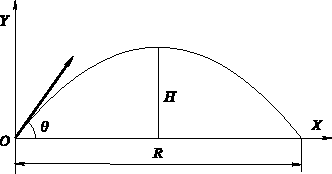
\includegraphics{figure/fig01.16}
 \caption{}
 \label{fig:01.16}
\end{wrapfigure}
因为当$\theta=\ang{45;;}$时,$\sin2\theta$
取最大值。所以,以同一速率$v_0$抛射物体,当
$\theta=\ang{45;;}$时,射程最远。
因为$\theta=\ang{90;;}$时,$\sin\theta$最
大,所以,只有当$\theta=\ang{90;;}$时,即竖直上抛,
$H$才能达到最大,其值为:
\begin{equation*}
 H_{\max }=\frac{v_{0}^{2}}{2 g}
\end{equation*}

这个题讨论的是理想情况,在实际情况中存在着空气阻力,
抛物速度愈大,阻力也愈大。空气阻力随着抛物速度的增加而逐
渐增加,在某一速度上将等于重力,这时物体将匀速下降。因而
实际上抛体的轨迹并不是理想的抛物线。

\section{圆周运动和角速度}\label{sec:01.09}

现在来讨论一种最简单的曲线运动——圆周运动。即轨迹是
个圆。如果选择圆心作为坐标原点,质点的位置就可用位置矢量
$\vec{r}$与某一选定的方向(例如$X$轴)之间的夹角$\varphi$(图\ref{fig:01.17})来描述,因
为$\varphi$确定之后,质点的位置就完全确定了。因而可用角$\varphi$与$t$的
关系$\varphi\left(t\right)$来代替函数$\vec{r}\left(t\right)$。

我们知道,对于直线运动,用一个坐标$x\left(t\right)$就可以描写。同
\clearpage
\noindent 样,对于圆周运动,也是只要一个坐标$\varphi\left(t\right)$来描写就够了。在这
\begin{wrapfigure}[9]{r}{13em}
  \centering \small
  
\includegraphics{figure/fig01.17}
  \caption{圆周运动}
  \label{fig:01.17}
\end{wrapfigure}
个意义上,两者是一样的。而一般的平面曲线运动,需要两个坐
标来描写;一般的空间曲线运动,则需要三个坐标来描写。我
们按描写运动所需坐标的个数,把运动分为一维运动、二维运动、
三维运动等等。直线运动和圆周运动都是一维运动。

按照\ref{sec:01.07}节的讨论,速度的
方向为轨迹上相应点的切线方向,圆的切线总与半径相垂直,所
以圆周运动的速度$\vec{v}$总与位置矢量$\vec{r}$相垂直。现在来求速度的

\begin{wrapfigure}[8]{l}{13em}
  \vspace{-0.5em}
  \centering \small
  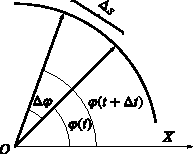
\includegraphics{figure/fig01.18}
  \caption{圆周运动的速率}
  \label{fig:01.18}
\end{wrapfigure}
\noindent 大小。由图\ref{fig:01.18},在$t$时刻,质点位于$\varphi\left(t\right)$;当$t+\Delta t$时,位于
$\varphi\left(t+\Delta t\right)$,所以在$\Delta t$间隔中质点
运动的路程为:
\setlength{\mathindent}{2em}
\begin{equation*}
  \begin{aligned}
    \Delta s & =r|\varphi\left(t+\Delta t\right)-\varphi\left(t\right)| \\
             & =r|\Delta \varphi|
  \end{aligned}
\end{equation*}
将此式代入式\eqref{eqn:01.07.05},就得到圆周运动的速率
\setlength{\mathindent}{6em}
\begin{equation}\label{eqn:01.09.01}
  v=\lim _{\Delta t \rightarrow 0} \frac{r|\Delta \varphi|}{\Delta t}=r \lim _{\Delta t \rightarrow 0} \frac{|\Delta \varphi|}{\Delta t}
\end{equation}
现在定义一个新的量,它是
\begin{equation}\label{eqn:01.09.02}
  \omega=\lim _{\Delta t \rightarrow 0} \frac{|\Delta \varphi|}{\Delta t}
\end{equation}
这种形式的公式我们已经多次遇到了。$|\Delta\varphi|/\Delta t$是在$t$到$t+\Delta t$间
隔中,质点的单位时间的角位置的平均变化。当取$\Delta t\rightarrow 0$的极限
时,这个平均变化率过渡为瞬时变化率。因此,我们称$\omega$为角速
度,确切地说,应称为角速率。它的单位是弧度/秒。利用角速率$\varphi$,式\eqref{eqn:01.09.01}可以写成
\begin{equation}\label{eqn:01.09.03}
  v=r\omega
\end{equation}

速度本质上是一个矢量,有大小和方向两方面。上述角速度
定义只反映了大小,为反映方向,我们需作些补充。

现在定义一个矢量$\vec{\omega}$,它的大小等于式\eqref{eqn:01.09.01}中的$\omega$,$ \vec{\omega}$的
方向按图\ref{fig:01.19}所示的方法给定。
\begin{figure}[!h]
  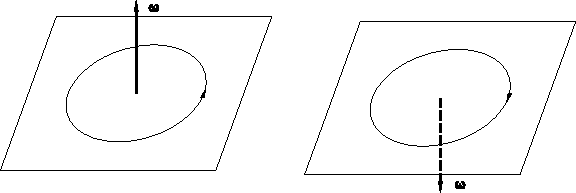
\includegraphics{figure/fig01.19}
  \caption{角速度的方向}
  \label{fig:01.19}
\end{figure}

\noindent 当我们从$ \vec{\omega}$指向的方向观察质点的运动时,质点总是沿逆时钟方
向转动。这个规定$ \vec{\omega}$的方向的方法也可以用一个正扣螺旋来说
明,当螺钉按质点运动方向旋转时,螺钉的运动方向就是$ \vec{\omega}$的方
向。

这样定义的$ \vec{\omega}$,称为角速度矢量。利用这个矢量。可以把质
点的速度矢量$\vec{v}$表示成
\begin{equation}\label{eqn:01.09.04}
  \vec{v}= \vec{\omega}\times \vec{r}
\end{equation}
由图\ref{fig:01.20},因为$ \vec{\omega}$与$\vec{r}$垂直,所以$| \vec{\omega}\times\vec{r}|=\omega r=v$,
而且$ \vec{\omega}\times\vec{r}$的方向与$\vec{v}$的方向一致。故式\eqref{eqn:01.09.04}
比\eqref{eqn:01.09.03}更具有一般性,它不仅表达了三者的大小关系,也反映了
三者间的方向关系。不仅如此,若取通过圆心且垂直于圆所在平面
的直线上任一点为原点(图\ref{fig:01.21})来描写圆周运动,式\eqref{eqn:01.09.04}仍成立,但式\eqref{eqn:01.09.03}就不对
\clearpage
\noindent 了。读者可以自己证明。

\begin{figure}[!h]
  \small
  \begin{minipage}[b]{15em}
    \centering
    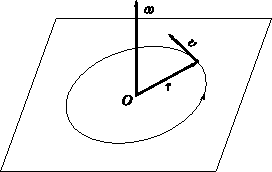
\includegraphics{figure/fig01.20}
    \vspace{4em}
    \caption{圆周运动中$ \vec{\omega}$与$\vec{v}$的关系}
    \label{fig:01.20}
  \end{minipage}
  \hfill
  \begin{minipage}[b]{13em}
    \centering
    
\includegraphics{figure/fig01.21}
    \caption{原点不在圆心的情况}
    \label{fig:01.21}
  \end{minipage}
\end{figure}


\section{匀速圆周运动}\label{sec:01.10}

一般情况角速率$\omega$是随$t$变化的,这时质点的速度的大小也
随$t$变化。以下讨论$\omega$不随$t$变化的特殊情况,即匀速圆周运动。
由式\eqref{eqn:01.09.03},这时质点的速率也不变化。质点绕圆周一圈走过的
路程是$2\uppi r$。如果走一圈所用时间为$T$,则质点的速率是
\begin{equation}\label{eqn:01.10.01}
  v=\frac{2 \uppi r}{T}
\end{equation}
T为周期,比较式\eqref{eqn:01.10.01}、\eqref{eqn:01.09.03},得到:
\begin{equation}\label{eqn:01.10.02}
  \omega=\frac{2 \uppi}{T}, ~ T=\frac{2 \uppi}{\omega}
\end{equation}
这也就是说,周期$T$等于质点转过$2\uppi$角度所需要的时间。

对于匀速圆周运动,$\vec{v}$的大小不变,而$\vec{v}$的方向时时在变,因
而它的加速度并不为零。由于速度方向总是垂直于矢量$\vec{r}$的,所
以在$t$到$t+\Delta t$间隔中,倘使$\vec{r}$转过角度$\Delta\varphi$,
则$\vec{v}$也就转过了$\Delta\varphi$。由于
$|\vec{v}\left(t\right)|=|\vec{v}\left(t+\Delta t\right)|=v$,由图\ref{fig:01.22}~的等腰三角形,得
\begin{equation*}
  \begin{aligned}
    |\vec{v}\left(t+\Delta t\right)-\vec{v}\left(t\right)| & =2 v \sin \frac{\Delta \varphi}{2}                   \\
                                                           & \approx 2 v\frac{\Delta \varphi}{2}=v \Delta \varphi
  \end{aligned}
\end{equation*}

\begin{figure}[!h]
  \small\centering
  \begin{minipage}[b]{14em}
    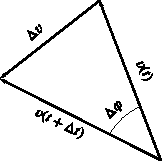
\includegraphics{figure/fig01.22}
    \vspace{1em}
    \caption{匀速圆周运动的加速度}
    \label{fig:01.22}
  \end{minipage}
  \begin{minipage}[b]{14em}
    \centering
    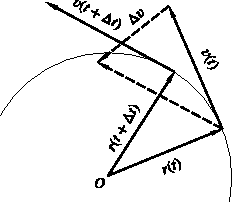
\includegraphics{figure/fig01.23}
    \caption{加速度的方向}
    \label{fig:01.23}
  \end{minipage}
\end{figure}
\noindent 将此式代入式\eqref{eqn:01.08.03},得
\begin{equation}\label{eqn:01.10.03}
  \begin{aligned}
    a & \equiv|\vec{a}|=\lim _{\Delta t \rightarrow 0} \frac{|\vec{v}\left(t+\Delta t\right)-\vec{v}\left(t\right)|}{\Delta t} \\
      & =v\lim_{\Delta t \rightarrow 0} \frac{|\Delta \varphi|}{\Delta t}=v \omega=r \omega^{2}=\frac{v^{2}}{r}
  \end{aligned}
\end{equation}\vspace{0.5em}
上式推导中利用了式\eqref{eqn:01.09.02},\eqref{eqn:01.09.03}。因为$v$或$\omega$都不随$t$变,
所以匀速圆周运动的加速度的大小也不随$t$变,但它的方向是时
时变化的。根据图\ref{fig:01.23},当$\Delta t\rightarrow 0$时,
$\vec{v}\left(t+ \Delta t\right)-\vec{v}\left(t\right)=\Delta\vec{v}$的方
向趋于与$\vec{v}\left(t\right)$相垂直,并指向圆心。这样,匀速圆周运动的加速
度的大小由式\eqref{eqn:01.10.03}给出,而其方向总是指向圆心的。根据这
种方向上的特点,称这个加速度为向心加速度。

速度、角速度和加速度都是矢量,我们可把式\eqref{eqn:01.10.03}扩充
为矢量关系式:
\clearpage
~\vspace{-1.56em}
\begin{equation}\label{eqn:01.10.04}
  \vec{a}= \vec{\omega}\times \vec{v}
\end{equation}
它的正确性也留给读者自己去证明。
\section{运动学里的反问题}\label{sec:01.11}

以上各节讨论的问题,都是当已知运动的轨迹函数$\vec{r}\left(t\right)$后,
求速度和加速度。在运动学中还会遇到一种相反的问题:已知质
点在各时刻的速度$\vec{v}\left(t\right)$,求它的轨迹函数$\vec{r}\left(t\right)$;已知加速度$\vec{a}\left(t\right)$,
求它的$\vec{v}\left(t\right)$。以前各节讨论的问题多与微分运算相联系,而这些
反问题,却是与积分运算相联系的。

仍然先讨论直线运动。如果已知直线运动的质点的速度为
$v\left(t\right)$,并已知在$t=0$时,质点在$x\left(0\right)$(称为初始位置),求在时刻
$t$的质点的坐标$x\left(t\right)$。

我们把零到$t$这段时间间隔,分成许多小段,即$\Delta t_1 , \Delta t_2 , \cdots$,
而且$\Delta t_1+\Delta t_2+\cdots=t$,如果所有各小段都相当小,则在每个间隔
中速度变化不太大,在$\Delta t_i$中速度近似为$v\left(t_i\right)$。这样,在每个时
间间隔中质点的坐标变化分别近似为:
\begin{equation*}
  \begin{array}{l}
    \Delta x_{1} \approx v\left(t_{1}\right) \Delta t_{1} \\[-1pt]
    \Delta x_{2} \approx v\left(t_{2}\right) \Delta t_{2} \\[-1pt]
    \cdots \cdots
  \end{array}
\end{equation*}
因而,质点在0到$t$间隔中坐标的总变化$x\left(t\right)-x\left(0\right)$就应当等于
这许多小变化的总和,即\vspace{-0.5em}
\begin{equation}\label{eqn:01.11.01}
  \begin{aligned}
    x\left(t\right)-x\left(0\right) & =\Delta x_{1}+\Delta x_{2}+\Delta x_{3}+\cdots    \\[-1pt]
                                    & \approx \sum_{i} v\left(t_{i}\right) \Delta t_{i}
  \end{aligned}
\end{equation}
各时间间隔$\Delta t_i$取得越小,计算结果就越准确,当所有$\Delta t_i\rightarrow 0$时,
就得到质点位置变化的精确值:

~\vspace{-1.56em}
\begin{equation}\label{eqn:01.11.02}
  x\left(t\right)=x\left(0\right)+\lim _{\Delta t_{i} \rightarrow 0} \sum_{i} v\left(t_{i}\right) \Delta t_{i}
\end{equation}
上式取极限的项,与积分的定义是一样的。所以它可写成
\begin{equation}\label{eqn:01.11.03}
  x\left(t\right)=x\left(0\right)+\int_{0}^{t} v\left(t\right) {~\mathrm d} t
\end{equation}
这就是我们所要求的答案。

现在说明式\eqref{eqn:01.11.01}或\eqref{eqn:01.11.02}中求和运算的几何意义。我
们在图\ref{fig:01.24}~中画出了速度$v$对时间$t$的关系曲线。各时间间隔$\Delta t_1 , \Delta t_2 , \cdots$,相应于横坐标上的各小段,各$v\left(t_1\right) , v\left(t_2\right) , \cdots$,相应
于各小段中$ v $的近似值。因而$\Delta x_1 , \Delta x_2 , \cdots$,在数值上就等于相
应的小长方形的面积。故对所有$\Delta x_i$求和,在各小段$\Delta x_i$都趋于
无限小的情况下,在数值上就等于零到$t$间横轴之上与曲线$v$之
下所围的面积。

利用这种几何性质,对一些简单情况,计算式\eqref{eqn:01.11.03}中的
积分是很容易的。下面举两个例子。

\begin{figure}[!h]
  \begin{minipage}[b]{14em}
    \centering
    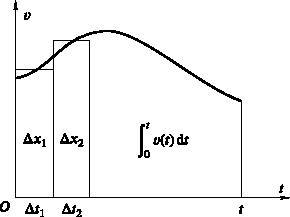
\includegraphics[width=0.8\linewidth]{figure/fig01.24}
    \caption{运动的$v-t$图}
    \label{fig:01.24}
  \end{minipage}\hfill
  \begin{minipage}[b]{14em}
    \centering
    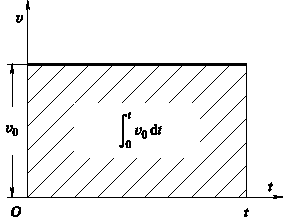
\includegraphics[width=0.8\linewidth]{figure/fig01.25}
    \caption{匀速运动的$v-t$图}
    \label{fig:01.25}
  \end{minipage}
\end{figure}

\setcounter{example}{0}
\example 匀速运动。

如果质点的速度是常数$v_0$,它的$v-t$图就如图\ref{fig:01.25}~所示。由0
到$t$的横轴与曲线$v$围成一个长方形,它的面积是$v_0t$,将之代入
式\eqref{eqn:01.11.03},即得轨迹函数为:
\begin{equation}\label{eqn:01.11.04}
  x\left(t\right)=x\left(0\right)+v_0 t
\end{equation}
~\vspace{-1.5em}
\begin{figure}[!h]
  \begin{minipage}[b]{14em}
    \centering
    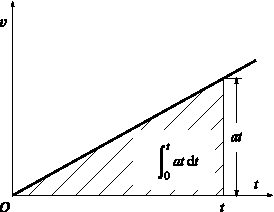
\includegraphics[width=0.8\linewidth]{figure/fig01.26}
    \caption{匀加速运动的$v \mathdash t$图}
    \label{fig:01.26}
  \end{minipage}\hfill
  \begin{minipage}[b]{14em}
    \centering
    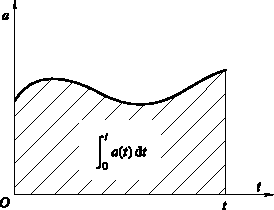
\includegraphics[width=0.8\linewidth]{figure/fig01.27}
    \caption{运动的$a-t$图}
    \label{fig:01.27}
  \end{minipage}
\end{figure}

\example 匀加速运动。

设质点的速度与时间成正比,$v=at$,在图\ref{fig:01.26}~中画出这个
关系。零到$t$的横轴与曲线$v$围成一个直角三角形,它的面积是
$\dfrac{1}{2} a t^2$,代入式\eqref{eqn:01.11.03},就得到轨迹函数为:
\begin{equation*}\label{eqn:01.11.04i}
  x\left(t\right)=x\left(0\right)+\frac{1}{2}at^2 \tag{1.11.4$'$}
\end{equation*}

已知加速度$a\left(t\right)$,求速度$v\left(t\right)$的方法,同样可以按上面的方
法求得,将0到$t$的时间间隔分成小段$\Delta t_1 , \Delta t_2 , \cdots$,每个小段中
加速度分别近似为$a\left(t_1\right) , a\left(t_2\right) , \cdots$,因而在每个小段中,速度的
变化相应为$\Delta v_1\approx a\left(t_1\right)\Delta t_1 , \Delta v_2\approx a\left(t_2\right)\Delta t_2 , \cdots$,在0到$t$间隔中速
度总的变化等于所有变化之和,即
\begin{equation}\label{eqn:01.11.05}
  \begin{aligned}
    v\left(t\right)-v\left(0\right) & =\Delta v_{1}+\Delta v_{2}+\cdots                 \\
                                    & \approx \sum_{i} a\left(t_{i}\right) \Delta t_{i}
  \end{aligned}
\end{equation}
其中$v\left(0\right)$是$t=0$时质点的速度,称为初速度。
同样,取所有$\Delta t _ i \to 0$的极限,就得到速度变化的精确表达式为:
\begin{equation}\label{eqn:01.11.06}
  \begin{aligned}
    v\left(t\right) & =v\left(0\right)+\lim _{\Delta t_{i} \rightarrow 0} \sum_ i a\left(t_{i}\right) \Delta t_{i} \\
                    & =v\left(0\right)+\int_{0}^{t} a\left(t\right) {~\mathrm d} t
  \end{aligned}
\end{equation}
上式中积分的几何意义是$a-t$图中由0到$t$的横轴与$a$曲线之间
所围的面积(图\ref{fig:01.27})。

对于曲线运动的情况,式\eqref{eqn:01.11.03}、\eqref{eqn:01.11.06}分别推广成
{\setlength{\mathindent}{4em}
%\setlength\abovedisplayskip{0pt}
%\setlength\belowdisplayskip{0pt}
%\setlength{\lineskip}{-1pt}
%\setlength{\lineskiplimit}{-1pt}
\begin{eqnarray}
  \label{eqn:01.11.07}
  \begin{aligned}
    \vec{r}\left(t\right)= & \vec{r}\left(0\right)+\int_{0}^{t} \vec{v}\left(t\right) {~\mathrm d} t \\
    =                      & \vec{r}\left(0\right)
    +\left(\int_{0}^{t} v_{x}\left(t\right) {~\mathrm d} t\right) \vec{i}
    +\left(\int_{0}^{t} v_{y}\left(t\right) {~\mathrm d} t\right) \vec{j}                            \\
                           & +\left(\int_{0}^{t} v_{z}\left(t\right) {~\mathrm d} t\right) \vec{k}
  \end{aligned} \\
  \label{eqn:01.11.08}
  \begin{aligned}
    \vec{v}\left(t\right)= & \vec{v}\left(0\right)+\int_{0}^{t} \vec{a}\left(t\right) {~\mathrm d} t \\
    =                      & \vec{v}\left(0\right)
    +\left(\int_{0}^{t} a_{x}\left(t\right) {~\mathrm d} t\right) \vec{i}
    +\left(\int_{0}^{t} a_{y}\left(t\right) {~\mathrm d} t\right) \vec{j}                            \\
                           & +\left(\int_{0}^{t} a_{z}\left(t\right) {~\mathrm d} t\right) \vec{k}
  \end{aligned}
\end{eqnarray}
\setlength{\mathindent}{6em}}%
其中$\vec{r}\left(0\right)$及$\vec{v}\left(0\right)$分别为初始时刻质点的位置矢量及速度矢量。具
体使用式\eqref{eqn:01.11.07}及\eqref{eqn:01.11.08}时,可以把它们分解成分量的关系
来计算。式\eqref{eqn:01.11.07}等价于下列三式。
{%\setlength\abovedisplayskip{0pt}
%\setlength\belowdisplayskip{0pt}
%\setlength{\lineskip}{-1pt}
%\setlength{\lineskiplimit}{-1pt}
\begin{equation}
  \begin{aligned}\label{eqn:01.11.09}
    x\left(t\right)=x\left(0\right)+\int_{0}^{t} v_{x}\left(t\right) {~\mathrm d} t \\
    y\left(t\right)=y\left(0\right)+\int_{0}^{t} v_{y}\left(t\right) {~\mathrm d} t \\
    z\left(t\right)=z\left(0\right)+\int_{0}^{t} v_{z}\left(t\right) {~\mathrm d} t
  \end{aligned}
\end{equation}}%
而式\eqref{eqn:01.11.08}等价于下列三式。
{%\setlength\abovedisplayskip{0pt}
%\setlength\belowdisplayskip{0pt}
%\setlength{\lineskip}{-1pt}
%\setlength{\lineskiplimit}{-1pt}
\begin{equation}\label{eqn:01.11.10}
  \begin{aligned}
    v_x\left(t\right)=v_x\left(0\right)+\int_{0}^{t} a_{x}\left(t\right) {~\mathrm d} t \\
    v_y\left(t\right)=v_y\left(0\right)+\int_{0}^{t} a_{y}\left(t\right) {~\mathrm d} t \\
    v_z\left(t\right)=v_z\left(0\right)+\int_{0}^{t} a_{z}\left(t\right) {~\mathrm d} t
  \end{aligned}
\end{equation}}%
这些积分中没有出现矢量,就可以按一般方法计算,譬如上述的
面积方法就是一种可行的方法.

研究运动有两种次序。一种是先研究轨迹,已知轨迹函数为
$\vec{r}\left(t\right)$,再来推求速度$\vec{v}\left(t\right)$,加速度$\vec{a}\left(t\right)$。就人类的认识过程来说,的
确是先看到轨迹的形状,然后有了运动快慢的概念,最后认识到
速度的变化,即加速度。另一种次序是:先知道加速度,然后再
求速度及轨迹。在物理学中,从力学的规律来看,往往是如此。

前一种次序,看上去非常自然,是人类研究机械运动所走的
一条路。在牛顿之前,亚里士多德认为轨迹是最基本的,速度则
次之。这种方法的特点是先研究运动的大的整体方面,然后再涉
及局部细节。

后一种次序,是牛顿创建的方法,也是现代物理学一个基本
的方法。牛顿认为,不要先探讨物体运动的整体方面。而是先研
究运动的瞬时情况,瞬时情况更为基本。弄清瞬时情况之后再来
讨论整体运动。也可以说,这种方法是先研究局部细节,然后再
作积分,得到整体性质。至今在大多数情况下,物理学家仍采取
牛顿的这种方法。

上述两种方法反映了两种不同的信念。一种认为整体的大的
方面更简单些,因此,主张从大到小的研究顺序;另一种认为局
部的单元过程更简单些,因此,主张从小到大的研究顺序。我们
将在第五章说明,这两种“简单性”可能是分不开的。

\begin{questions}

  \question 一个原则上不能进行直接或间接测量的物理量是否有意
  义?

  \question 平均速率有两种意思,一是指平均速度矢量的大小,一
  是指物体运动路径总长度除以所用的总时间。这两种意思是否相
  同?

  \question 质点作一维运动,如果加速度不是恒量,质点的平均速率
  是否等于$\dfrac 1 2$(初速+末速)?

  \question 当物体的加速度恒定不变时,它的运动方向可否改变?

  \question 质点的运动方程为$x=x\left(t\right)$,$y=y\left(t\right)$。在计算它的速度和
  加速度的大小时,有人先求出$r=\sqrt{x^2+y^2}$,然后根据$v=\dfrac{ \dif r}{ \dif t}$,
  $a=\dfrac{ \dif ^2r}{ \dif t^2}$,求得结果;有人先计算速度和加速度分量,再合成,所
  得结果为:\vspace{-1em}
  \begin{equation*}
    \begin{aligned}
      v & =\sqrt{\left(\frac{ \dif  x}{ \dif  t}\right)^{2}+\left(\frac{ \dif  y}{ \dif  t}\right)^{2}}                 \\
      a & =\sqrt{\left(\frac{ \dif ^{2} x}{ \dif  t^{2}}\right)^{2}+\left(\frac{ \dif ^{2} y}{ \dif  t^{2}}\right)^{2}}
    \end{aligned}
  \end{equation*}
  你认为哪一组结果正确?

  \question  两千多年前,住在尼罗河口亚历山大城的埃拉托色尼,首
  估算出地球的半径。然而,真正沿着地球子午线用绳长及日晷对
  地球进行测量的,却是中国唐代高僧一行(公元683$\sim$727)。你知
  道高僧一行测量的原理,方法及计算结果吗?

  \question  设想将一小球上抛。如不考虑空气阻力,试证明它返回原
  地时的速率等于开始的速率,并证明上升和下落所经过的时间相
  等。

  \question  将一小球铅直地上抛,若考虑空气阻力,它上升和下降所
  经过的时间哪一个长?

  \question  假设有两石块$m$和$M$,其中$m$较轻,$M$较重。按照亚里士多
  德的看法,在地面上$M$应该比$m$下落得快些。伽利略首先用思辨
  的方式指出亚里士多德的看法是自相矛盾的。伽利略说,设想将
  $m$与$M$系在一起,则构成物体$\left(m+M\right)$,此物下落时,因为$m$有下
  落得较慢的趋势,所以,$m$应该阻碍$M$,使它下落得比$m$快些而又
  比$M$慢些;但是另一方面,物体$\left(m+M\right)$比$M$还要重,按照亚里
  士多德的看法,它应比$M$下落得更快。因此,导致矛盾。

  你认为伽利略的推理是否正确?

  \question  质点在空间的运动,一般是三维运动。忽略风的作用的抛
  体运动,为什么可以作为二维运动来处理?
\end{questions}

\begin{exercises}

\exercise 用芝诺时计算阿基里斯的速度$v_1'$和加速度$a_1'$,并给出$x \mathdash t'$图。

\exercise 甲乙两列火车在同一水平直路上以相等的速率(30公里/时)
相向而行。当它们相隔60公里的时候,一只鸟以60公里/时的
恒定速率离开甲车头向乙车头飞去,一当到达立即返回,如此来
回往返不止。试求:

(1)当两车头相遇时,鸟往返了多少次?

(2)鸟共飞行了多少时间及距离?

(3)我们定义一种特殊的“小鸟钟”:小鸟从一车头到另一车
头为小鸟钟的时间测量单位(即小鸟钟的一个“滴答”)。用小鸟
钟记时的数值为$t''$求$t''$与一般时钟记时$t$之间的变换。

\exercise 一人从$O$点出发,向正东走3.0米,又向正北走1.0米,
\begin{wrapfigure}[8]{r}{8.5em}
 \begin{center}
 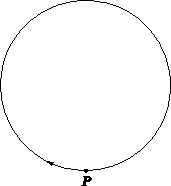
\includegraphics{figure/fig01.28}
 \caption{}
 \label{fig:01.28}
 \end{center}
\end{wrapfigure}
然后向东北走2.0米,试求合位移的大小及方向。

\exercise 一质点从$ P $出发,向左以匀速率1.0厘米/秒沿半径为$R=1.0$米的圆周运动(图\ref{fig:01.28})。问:

(1)当它走过2/3圆周时,位移是多少?走过的路程是多少?在这段时间内的
平均速度是多少?该点的瞬时速度是多少?

\clearpage
(2)当它走过1/2圆周时,以上各值又如何?

\exercise 一物体作直线运动,它的位置由方程$x=10t^2+6$决定,其
中$x$的单位为厘米,$t$的单位为秒,试计算:

(1)在$ 3.00\sim 3.10 $秒、$ 3.000\sim 3.01 $秒及$ 3.000\sim 3.001 $秒间
隔内的平均速度;

(2)在$t=3.00$秒时的瞬时速度;

(3)用微分方法求它的速度及加速度公式。

\exercise 有一质点沿x方向作直线运动,t时刻的坐标为:
\begin{equation*}
 x=4.5t^2-2t^3
\end{equation*}
式中$x$的单位为米。$t$的单位为秒。试求:

(1)第2秒内的位移和平均速度;

(2)第1秒末和第2秒末的瞬时速度;

(3)第2秒内质点所走过路径的长度;

(4)第2秒内的平均加速度以及第0.5秒末和第1秒末的瞬时
加速度。

\exercise 一质点以恒定的径向速度$r=4$米/秒在一平面中运动。它
的角速度为常量,其大小为$\omega=\dot\theta=2$弧度/秒。当质点距原点为3
米时,它的速度的大小及加速度大小是多少?

\exercise 如图\ref{fig:01.29}~所示,向上抛一物体,测量物体上抛及下落经
\begin{wrapfigure}[10]{r}{13em}
 \begin{center}
 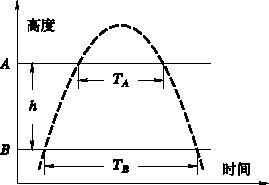
\includegraphics{figure/fig01.29}
 \caption{}
 \label{fig:01.29}
 \end{center}
\end{wrapfigure}
过水平线$A$的时差$T_A$,以及上抛
及下落经过水平线$B$的时差$T_B$。
试证明,若忽略空气阻力,重力
加速度的大小可以表示为:
\begingroup
\setlength{\mathindent}{4em}
\begin{equation*}
 g=\dfrac{8h}{T_A^2 - T_B^2}
\end{equation*}
\endgroup
式中$h$是$B$线与$A$线的高度差。

\exercise 天体物理常涉及大尺度的
问题,为了方便起见,引进一些
实用的大的长度单位。一个天文单位(AU)等于从地球到太阳的
平均距离;一个秒差距是一个天文单位所张之角为1秒的距离,即
观测者从某一恒星看地球公转轨道半径所张的角度为1秒时,该恒
星与太阳之间的距离。试求。

(1) 1秒差距相当于多少米?多少天文单位?及多少光年?

(2)以秒差距为单位,表示地球到太阳的距离。

\exercise 一物体从离地面的高度为$ h $的地方,由静止开始自由下
落,经过最后196米所用的时间是4.0秒钟。求物体下落过程所用
的总时间及其高度。

\exercise 一枚从地面发射的火箭以20米/$\text{秒}^2$的匀加速度竖直上升
半分钟后,燃料用完,于是象一个自由质点一样运动。略去空气
阻力,试求。

(1)火箭达到的最大高度;

(2)它从离开地面到再回地面所经过的总时间。

\exercise 把两个小物体从同一地点以同样初速率$v_0=24.5$米/秒
先后竖直上抛,设抛出两物体的时差为$\Delta t=0.500$秒,试问:

(1)第二个物体抛出后,经过多少时间$t$才与第一个物体相遇?

\vspace{-0.15em}(2)如果$\Delta t\geqslant\dfrac{2v_0}{g}$,讨论结果的物理意义。\vspace{-0.15em}

\exercise 物体以初速$v_0=20$米/秒被抛出,抛射仰角是\ang{60;;},略去
空气阻力,试问:

(1)物体开始运动后的1.5秒末,运动方向与水平方向的夹角
$\alpha$是多少?2.5秒末夹角$\alpha$又为多少?

(2)物体抛出后经过多少时间,运动方向才与水平成\ang{45;;}角?
这时物体的高度是多少?

(3)在物体轨迹最高点处的曲率半径$R_1$有多大?

(4)在物体落地点处,轨迹的曲率半径$R_2$有多大?

\exercise 高台下降滑雪在一平滑的山坡上进行。山坡与水平线成
恒定角度$\alpha$,滑雪运动员初速率为$v_0$,并以与水平线成$\theta$的仰角跳
出(\ref{fig:01.30})。若不考虑空气阻力,试证明:
\begin{figure}[h]
 \centering
 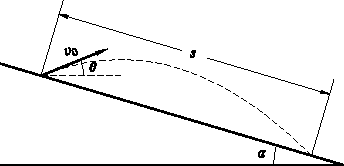
\includegraphics{figure/fig01.30}
 \caption{}
 \label{fig:01.30}
\end{figure}

(1)运动员落在斜坡上的距离为:
\begin{equation*}
 s=\frac{2 v_{0}^{2} \sin \left(\theta+\alpha\right) \cos \theta}{g \cos ^{2} \alpha}
\end{equation*}

(2)对于一定的$v_0$和$\alpha$来说,$s$在$\theta=\ang{45;;}-\dfrac{\alpha}{2}$时有最大值。其
值为:
\begin{equation*}
 s_{\max }=\frac{v_{0}^{2}\left(1+\sin \alpha\right)}{g \cos ^{2} \alpha}
\end{equation*}

\exercise 1977年中国男子铁饼的最好记录是54.28米,1983年提高
到60米。这些记录都是在北京创造的,北京的重力加速度$g$为
980.12厘米/$\text{秒}^2$。设投掷点比落地点高1.5米,略去空气阻力,
问投掷时至少要用多大的初速度,才可达到上述距离?

\exercise 设若干个光滑斜面($a_1, a_2, a_3, \dots $)有共同的底边$b$为30
厘米。试问:

(1)斜面与水平夹角$\alpha$为多大时,才能使物体在该斜面上从顶
端自由滑至底上正好需时为$t=0.4$秒?

(2)多大的夹角$\alpha$,使下滑的时间最短?

\exercise 在空间某一点$O$以相同的速率向各方向同时把若干小
球搬出去。试证明在略去空气阻力的情况下,任一时刻$t$,所有小
球都位于一个球面上,并求:

(1)此球心的运动方程式;

(2)球面距球心的距离。

\exercise 若抛射体的初速率为$v_0$,抛射角为$\theta$,略去空气阻力。伽
利略说:“抛射角为$\ang{45;;}+\delta$和$\ang{45;;}-\delta\left(\delta<\ang{45;;}\right)$的两个抛射体初速
率相同时,射程是相等的。”试证明他的话,并证明$\theta=\ang{45;;}$时水
平射程最大。

\begin{wrapfigure}[8]{r}{13em}
 \vspace{-2.5em}
 \begin{center}
 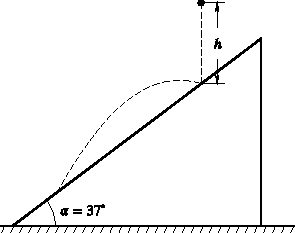
\includegraphics{figure/fig01.31}
 \caption{}
 \label{fig:01.31}
 \end{center}
\end{wrapfigure}
\exercise 一弹性球自由下落在一斜面上,与斜面发生完全弹性碰
撞,下落高度$h=20$厘米,斜面对水平的倾角$\alpha=\ang{37;;}$(图\ref{fig:01.31})。若
不计空气阻力,它第二次碰到斜面的位置距原来的下落点多远?

\exercise 用枪瞄准空中的靶,当子弹射出枪口时,靶同时自由下
落。如果略去空气阻力。不论子弹速率多大,总会击中下落的靶,
这个现象叫做百发百中,说明其中理由。

\exercise 一轰炸机高海面10公里,以240公里/小时的水平速度追
击正前方一鱼雷艇,鱼雷艇的速度是95公里/小时,不计空气阻
力,问飞机应在艇后多少距离投弹才能正好击中目标?

\exercise 一俯冲轰炸机沿与铅垂线成$\ang{37;;}$方向俯冲,在800米高度
投弹,炸弹离开飞机5.0秒钟时着地。不计空气阻力,试问:

(1)飞机的飞行速度是多少?

(2)炸弹离开飞机后在水平方向前进多远?

(3)炸弹着地时,速度的大小和方向?

\exercise 应以多大的水平速度$v$把一物体从高$h$处抛出,才能使
它在水平方向的射程为$h$的$n$倍?

\exercise 飞机以360公里/小时的速度由东向西飞行。试回答:

(1)在什么地理纬度上,飞机上的人可以看见太阳不动地停
在空中?

(2)若在极地附近沿纬线以圆轨道由东向西飞行,可以看见
什么现象?

\exercise 一俯冲轰炸机以不变的速率450公里/小时俯冲后。急离
俯冲线改为沿一铅垂平面内的圆形路线飞行。试问:要使飞机在
圆的最低点的加速度不超过$7g$,圆形路线的最小半径应是多少?

\exercise 车轮在地平面上作匀角速的纯滚动,轮行的速度为$v_0=
 10$米/秒,轮的半径为$r=0.50$米,试求;

(1)车轮边缘上一点$A$的角速度$\omega$;

(2)$A$点的轨迹。

\exercise 一半径为$r$的小球沿两固定的等高平行导轨作纯滚动,
两导轨间的距离为$d$,如图\ref{fig:01.32}~所示。试问:

(1)球心的速度与球的角速度的关系是怎样的?

(2)小球面上一点$A$的轨迹如何?
\begin{figure}[h]
 %\vspace{-1em}
 \begin{center}
 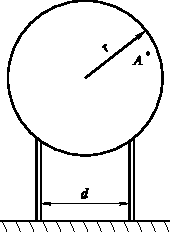
\includegraphics{figure/fig01.32}
 \caption{}
 \label{fig:01.32}
 \end{center}
\end{figure}

\end{exercises}


% 第二章
\chapter{运动学中的相对性}\label{chp:02}

\section{相对和绝对}\label{sec:02.01}

人对自然界认识的深化,常常是和弄清什么是相对的、什么
是绝对的这类问题联系在一起的。

远古时期,无论在东方文明或西方文明中,都认为大地是平
坦的,天在大地的上面。“天圆地方”就是这种观念的通俗表
述。用现代语言来说,在这种观念中,“上”“下”这两个方向是
绝对的。

到古希腊时期,毕达哥拉斯以及亚里士多德等先后开始主张
大地是一个球体,即地球。中国的“浑天说”也有大体相似的观
念。这是认识上的一次进步,因为它抛弃了当时的一种“习惯”
的但却不正确的观念——“上”“下”是绝对的。

按照当时“习惯”的看法,如果大地是球形,那些居住在我们
的对蹠点上的人不是早就“掉下”去了吗?可见,树立球形大地
观需要克服一些不正确的成见所带来的阻力。因此,从相对与绝
对角度来评价,可以说,地球观是把“上”和“下”这两个方向
相对化了。我们看对照点的人在“下”,对照点的人看我们也是
在“下”,亦即空间各个方向是等价的,没有一个方向具有特别
的绝对优越的性质。

在亚里士多德的体系中,认为地球的球心是宇宙的中心。这
个位置具有非常特殊的,绝对的意义。亚里士多德还认为,物体
运动的规律是力图达到自己的天然位置,地面附近物体的天然位
置就是地球的中心,远处物体(如星体)则应环绕着地球的中心。
这样,在支配物体运动的规律中,空间位置具有特别的作用,这
种性质,可以叫做空间位置的绝对性。

以牛顿力学为起点的物理学,否定了亚里士多德体系中的空
间位置的绝对性,认为任何的空间点都是平权的,地心在宇宙中
并不占有特殊的地位。牛顿理论中的相对和绝对,又不同于亚里
士多德了。

正因为相对和绝对这一问题的重要性,在这一章里,我们将
系统地分析一下牛顿的运动学中的相对性,并且还将指出,牛顿
体系中的相对绝对观也是有局限的,在某些条件下,就完金不适
用了。
\section{位置和轨迹的相对性}\label{sec:02.02}

在运动学中,最基本的概念是位置。由图\ref{fig:02.01}~看到。对于质点
$P$,相对于参考系$K$而言,它的位置矢量是$\vec{OP}$,即
\begin{equation*}
  \vec{OP}=x\vec{i}+y\vec{j}+z\vec{k}
\end{equation*}
同时,相对于参考系$K'$来说,它的位置矢量是$\vec{O'P}$,即
\begin{equation*}
  \vec{O'P}=x'\vec{i'}+y'\vec{j'}+z'\vec{k'}
\end{equation*}
\begin{figurex}
  \centering
  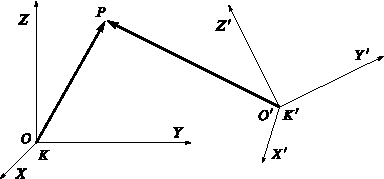
\includegraphics{figure/fig02.01}
  \caption{位置的相对性}
  \label{fig:02.01}
\end{figurex}

\clearpage
可见同一质点的位置,对不同的参考系,可用不同的位置矢量来
描写,这就是位置描写中的相对性。

从描写质点位置来说,选用参考系$ K $或者$ K' $,是等价的。因
为参考系$K$及$K'$一旦选定,它们之间的关系就完全确定了。我们
知道了质点在参考系$K$中的位置坐标$\left(x,y,z\right)$,就可求得在参考
系$K'$中的位置坐标$\left(x,y,z\right)$,反之亦然。用数学语言来说,
即$x,y,z$与$x',y',z'$之间有确定的变换关系:
\begin{align}
  \label{eqn:02.02.01}
   & \left\{\begin{array}{l}
              x'=x'\left(x, y, z\right) \\
              y'=y'\left(x, y, z\right) \\
              z'=z'\left(x, y, z\right)
            \end{array}\right.  \\
  \label{eqn:02.02.02}
   & \left\{\begin{array}{l}
              x=x\left(x', y', z'\right) \\
              y=y\left(x', y', z'\right) \\
              z=z\left(x', y', z'\right)
            \end{array}\right.
\end{align}
式\eqref{eqn:02.02.01}、\eqref{eqn:02.02.02}~称为坐标变换。

现在我们介绍几种物理学中常用的坐标变换。

\begin{wrapfigure}{r}{16em}
  \centering
  
\includegraphics{figure/fig02.02}
  \caption{空间平移}
  \label{fig:02.02}
\end{wrapfigure}
\textsf{1. 坐标平移}

如图\ref{fig:02.02},参考系$K$及$K'$的$X$轴与$X'$轴重合,$Y$轴与$Y'$轴平行,
$Z$轴与$Z'$轴平行,原点$P$的坐标在参考系$K$及$K'$中分别是$x,y,z$和
$x',y',z'$,显然,坐标变换是:
\begin{equation}\label{eqn:02.02.03}
  \left\{\begin{array}{l}
    x=x'+d \\
    y=y'   \\
    z=z'
  \end{array}\right.
\end{equation}

\begin{wrapfigure}{r}{15em}
  \centering
  
\includegraphics{figure/fig02.03}
  \caption{空间转动}
  \label{fig:02.03}
\end{wrapfigure}
\textsf{2. 坐标转动}

讨论平面问题时,取如图\ref{fig:02.03}~的参考系$K$及$K'$,它们的原点$O$与$O'$重合,参考
系$K'$的轴相对于参考系$ K $转动一个$\theta$角。质点$P$的位置坐标在参考系$K$,
$K'$中分别是$x,y,z$和$x',y',z'$。不难求出,此时的坐标变换是:\vspace{-0.2em}
\begin{equation}\label{eqn:02.02.04}
  \left\{\begin{array}{l}
    x=x'\cos\theta-y'\sin\theta \\
    y=x'\sin\theta+y'\cos\theta
  \end{array}\right.
\end{equation}
或\vspace{-1em}
\begin{equation*}
  \left\{\begin{array}{l}
    x'=x\cos\theta+y\sin\theta \\
    y'=x\sin\theta-y\cos\theta
  \end{array}\right.
\end{equation*}

\begin{wrapfigure}{r}{15em}
  \centering
  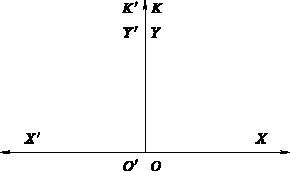
\includegraphics{figure/fig02.04}
  \caption{空间反演}
  \label{fig:02.04}
\end{wrapfigure}
\textsf{3. 空间反演}

如图\ref{fig:02.04},参考系$K$与$K'$的原点$O$与$O'$重合,$Y$轴与$Y'$轴重合,而$X$轴与
$X'$轴反向。这时,坐标变换是:\vspace{-0.5em}
{\setlength{\mathindent}{2em}
  \begin{equation}\label{eqn:02.02.05}
    \left\{\begin{array}{l}
      x=-x' \\
      y=y
    \end{array}\right.
  \end{equation}}%

弄清了位置的相对性,关于轨迹的相对性也就不难理解了。

质点运动的轨迹,一般来说是一条空间曲线。对于一个质点
的轨迹,相对于参考系$ K $,我们可用曲线方程
\begin{equation}\label{eqn:02.02.06}
  \left\{\begin{array}{l}
    f_1\left(x,y,x\right)=0 \\
    f_2\left(x,y,z\right)=0
  \end{array}\right.
\end{equation}
来描写;也可相对于参考系$K'$,用曲线方程

~\vspace{-1.56em}
\begin{equation}\label{eqn:02.02.07}
  \left\{\begin{array}{l}
    f'_1\left(x',y',x'\right)=0 \\
    f'_2\left(x',y',z'\right)=0
  \end{array}\right.
\end{equation}
来描写。一般说来,函数形式$f_1,f_2$和式$f'_1,f'_2$是不相同的,这
就是轨迹的相对性。将式\eqref{eqn:02.02.02}~代入式\eqref{eqn:02.02.06},就可由$f$求得
$f'$;将式\eqref{eqn:02.02.01}~代入式\eqref{eqn:02.02.07},就可由$f'$求得$f$。

作为示例,我们讨论两个平面运动。有两个质点。它们相对
于参考系$K$的运动轨迹分别由下列曲线方程描写:
\begin{align}
  x-ky    & =0  \label{eqn:02.02.08}  \\
  x^2+y^2 & =r^2 \label{eqn:02.02.09}
\end{align}
式\eqref{eqn:02.02.08}~表示一直线运动,式\eqref{eqn:02.02.09}~表示中心在原点,半径
为$r$的一个圆周运动。

现在取另一参考系$K'$,它仅相对于参考系$K$转了一个$\theta$角。
我们把式\eqref{eqn:02.02.04}代入式\eqref{eqn:02.02.08},整理后得
{\setlength{\mathindent}{4em}
\begin{equation}\label{eqn:02.02.10}
  x'\left(\cos\theta - k\sin\theta\right)-y'\left(\sin\theta + k\cos\theta\right)=0
\end{equation}}%
式\eqref{eqn:02.02.10}~就是在参考系$K'$中所看到的第一个质点的轨迹方程,
它也是一条直线,但斜率与式\eqref{eqn:02.02.08}不同。
将式\eqref{eqn:02.02.04}~代入式\eqref{eqn:02.02.09},得
\begin{equation}\label{eqn:02.02.11}
  x'^2+y'^2=r^2
\end{equation}
由式\eqref{eqn:02.02.11}~看到,第二个质点的轨迹相对于参考系$K'$,也是中
心在原点。半径为$r$的圆。

如果一种运动轨迹相对于两参考系形状相同。而且它与两坐
标系的关系也一样,我们称这种特殊轨迹对于这一特定的坐标变
换具有不变性。用数学语育来说,当参考系$K$变到$K'$时。若轨迹
方程由
\begin{equation*}
  f\left(x,y,z\right)=0
\end{equation*}
变换成
\begin{equation*}
  f\left(x',y',z'\right)=0
\end{equation*}
它就是具有不变性的轨迹。由此可见,第一个质点轨迹相对于坐
标转动变换并不具有不变性,而第二个质点轨迹对于坐标转动变
换是有不变性的。

下面讨论涉及时间的变换,坐标系$K$及$K'$所用的时间$t$及$t'$
也可以是不相同的。最常遇到的一种时同变换,是所谓时间平移,
即$t=t'+t_0$,也就是$K$及$K'$的时间坐标的原点相差一常数$t_0$。
譬如,在参考系$K$中用东京时间,在参考系$K'$中用北京时间,
那么,常数$t_0$就等于1小时。

如果在参考系K中,轨迹函数是\vspace{-0.2em}
\\\null\hspace{6em}$x=x\left(t\right)$
\\\null\hspace{6em}$y=y\left(t\right)$
\\\null\hspace{6em}$z=z\left(t\right)$\\
我们很容易推知,在参考系$K'$中,轨迹函数是\vspace{-0.2em}
\\\null\hspace{6em}$x=x\left(t'+t_0\right)$
\\\null\hspace{6em}$y=y\left(t'+t_0\right)$
\\\null\hspace{6em}$z=z\left(t'+t_0\right)$

另一种时间变换在日常生活中不常见,但在物理上非常有用。
那就是\vspace{-0.5em}
\\\null\hspace{6em}$t=-t'$\\
它表示当$K$中的时间走向将来时,$K'$相应的时间却走向过去。因
此,称这种时间变换为时间倒转。

我们不难由参考系$K$中的轨迹函数\vspace{-0.2em}
\\\null\hspace{6em}$x=x\left(t\right)$
\\\null\hspace{6em}$y=y\left(t\right)$
\\\null\hspace{6em}$z=z\left(t\right)$\\
得到相应在参考系$K'$中的轨迹函数为\vspace{-0.2em}
\\\null\hspace{6em}$x=x\left(-t'\right)$
\\\null\hspace{6em}$y=y\left(-t'\right)$
\\\null\hspace{6em}$z=z\left(-t'\right)$

为了弄清时间倒转的物理意义,我们举一个直线运动的例子
(图\ref{fig:02.05})。质点沿$X$轴运动。在参考系$K$中看,$t=1$时,质点在$x_1$;
$t=2$时,在$x_2$;显然,质点是从左向右运动的。但在参考系$K'$中看,
质点在$x_1$时,$t'=-1$;在$x_2$时,$t'=-2$;由于时间$t'=-2$比$t'=-1$
早,而时间总是从过去向将来发展,因此,相对于参考系$K'$,质
点是从右向左运动的。
\begin{figurex}
  \centering
  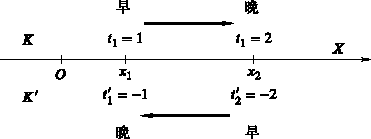
\includegraphics{figure/fig02.05}
  \caption{时间倒转}
  \label{fig:02.05}
\end{figurex}

\section{速度的相对性}\label{sec:02.03}

我们首先讨论质点的直线运动。

取参考系$K$和$K'$的$X$轴都和质点轨迹重合,而两原点$O$、$O'$
相距为$d$(图\ref{fig:02.06})。由式\eqref{eqn:02.02.03}知,$K,K'$之间的坐标变换是
\begin{equation*}
  x'=x-d
\end{equation*}
现在,若$K'$相对于$K$以均匀速率$u$沿$X$正向运动,则有
\begin{equation*}
  d=ut+d_0
\end{equation*}
\vspace{-1.56em}
\begin{figure}[h]
  \centering
  
\includegraphics{figure/fig02.06}
  \caption{速度的相对性}
  \label{fig:02.06}
\end{figure}

\noindent 其中$d_0$是时间$t=0$时,坐标原点$O$,$O'$间的距离。故坐标变换
公式为
\begin{equation}
  x'=x-ut-d_0 \label{eqn:02.03.01}
\end{equation}

有了式\eqref{eqn:02.03.01},就不难讨论$K$,$K'$之间的变换关系。

设在$K$系中,质点轨迹函数为
\begin{equation*}
  x=x\left(t\right)
\end{equation*}
根据定义,质点相对于$ K $系的速度为
\begin{equation*}
  v\left(t\right)\equiv\frac{\dif x}{\dif t}
\end{equation*}

相对于$K'$系,由式(2.3.1),质点的轨迹函数应为
\begin{equation*}
  x'=x'\left(t\right)=x\left(t\right)-ut-d_0
\end{equation*}
按照定义,质点相对于$K'$的速度为
\begin{equation*}
  v\left(t\right) \equiv\frac{\dif x'}{\dif t}=\frac{\dif x}{\dif t}-u
\end{equation*}
\begin{align}
  \beforetext{即} v'=v-u \label{eqn:02.03.02}
\end{align}
式\eqref{eqn:02.03.02}就是同一质点相对于$K$及$K'$二者的速度之间的关系。

\begin{wrapfigure}[9]{r}{14.5em}
    \vspace{-0.7em}
  \centering
  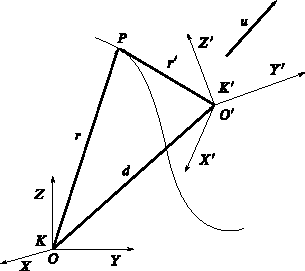
\includegraphics{figure/fig02.07}
  \caption{相对作匀速运动的$K$及$K'$}
  \label{fig:02.07}
\end{wrapfigure}
现在把式\eqref{eqn:02.03.02}推广到三维情况。

由图\ref{fig:02.07}~知,在$K$及$K'$中,质点$P$的位置分别用$\vec{r}$,
$\vec{r'}$表示。它们之间的关系是
{\setlength{\mathindent}{4em}
\begin{equation*}
  \vec{r'}=\vec{r}-\vec{d}
\end{equation*}}%
如果$K'$系相对于$K$系以均匀速度$\vec{u}$运动,则有
{\setlength{\mathindent}{4em}
\begin{equation*}
  \vec{d}=\vec{u}t+\vec{d}_0
\end{equation*}}%
其中$\vec{d}_0$是时刻$t=0$时,从$O$到$O'$的矢量。故有
  \begin{equation}
    \vec{r}'=\vec{r}-\vec{u}t-\vec{d}_0 \label{eqn:02.03.03}
  \end{equation}
若在$K$系中,质点的轨迹函数是

~\vspace{-1.5em}
  \begin{equation*}
    \vec{r}=\vec{r}\left(t\right)
  \end{equation*}
  则根据定义,质点相对于$K$的速度是
  \begin{equation}\label{eqn:02.03.04}
    \vec{v}\left(t\right)\equiv\frac{\dif \vec{r}}{\dif t}
  \end{equation}
  另一方面,由式\eqref{eqn:02.03.03}~可以求出质点在$K'$系中的轨迹函数,它是
  \begin{equation*}
    \vec{r}'=\vec{r}'\left(t\right)=\vec{r}\left(t\right)-\vec{u}t-\vec{d}_0
  \end{equation*}\label{err:02.03.02}
  因此,质点相对于$ K' $的速度是
  \begin{equation}\label{eqn:02.03.05}
    \vec{v}'\left(t\right)\equiv\frac{\dif \vec{r}'}{\dif t}=\frac{\dif \vec{r}}{\dif t}-\vec{u}
  \end{equation}
  \begin{align}\label{eqn:02.03.06}
    \beforetext{即} \vec{v}'=\vec{v}-\vec{u}
  \end{align}
  式\eqref{eqn:02.03.06}就是三维情况的速度变换公式,又称速度合成公式。可
  见,在不同参考系中,同一运动可能具有不同速度,亦即速度是
  具有相对性的概念。

  \begin{wrapfigure}{r}{17em}
    \vspace{-1em}
    \centering
    
\includegraphics{figure/fig02.08}
    \caption{}
    \label{fig:02.08}
  \end{wrapfigure}
  \example 一人向东以$v_1=50\text{米/分}$的速度运动,他觉得风从正南
  方吹来。假若人行速度增至$v_1'=75\text{ 米/分}$,他觉得风从东南方吹来。
  求风的速度$\vec{v}$。

  \solution 设两次感觉到的风速为$\vec{v}_2$和$\vec{v}_2'$。根据题意,各个速度应有以下关系:
  \begin{align*}
    \vec{v}_1+\vec{v}_2=\vec{v} \tag{1} \label{xeqn:02.03.01} \\
    \vec{v}_1'+\vec{v}_2'=\vec{v} \tag{2} \label{xeqn:02.03.02}
  \end{align*}
  作出矢量图(图\ref{fig:02.08})由式\eqref{xeqn:02.03.01}知$\vec{v}$的末端在$l_1$上,由式\eqref{xeqn:02.03.02}知$\vec{v}$的
  末端在$l_2$上,故$l_1$和$l_2$的交点是$\vec{v}$的末端。显然有:
  \begin{equation*}
    v_1=v_1'-v_1=76-50=25\text{ 米/分}
  \end{equation*}

  ~\vspace{-1.2em}
  \begin{align*}
    v      & =\sqrt{v_1^2+v_2^2}=\sqrt{50^2+25^2}=25\sqrt{25}\text{ 米/分} \\
    \theta & =\arctg\frac{v_2}{v_1}=\arctg\frac{25}{50}=\ang{26;35;}
  \end{align*}
  从而可看到不同参考系中能感觉到不同的风速。在地球参考系中
  风速是$\vec{v}$,以50米/分向东行走的人感觉风速是$\vec{v}_2$;而以75米/分向
  东行走的人则感觉到风速是$\vec{v}_2'$。

  \example 一列火车以速度$\vec{v}_1$沿水平直轨运行。车上有人以初
  速度$\vec{v}_2$竖直向上抛出一小球。车上及地面各站一人研究小球的运
  动。在不计空气阻力情况下,不同观察者看到速度,加速度及轨
  迹有何不同?

  \solution (1)以车为参考系。

  因为\vspace{-1em}
  \begin{align*}
     & \vec{v}=\vec{v}_x+\vec{v}_y=v_x\vec{i}+v_y\vec{j} \\
     & v_x=0,~ v_y=v_2-gt
  \end{align*}
  \begin{align*}
     \beforetext{所以} & \vec{v}=\left(v_2-gt\right)\vec{j} \\
     & |\vec{v}|=v_2-gt
  \end{align*}
  运动在铅直线上进行,是竖直上抛运动;加速度是重力加速度$g$。

  (2)以地心为参考系。

  因为\vspace{-1em}
  \begin{equation*}
    \vec{v}=\vec{v}_x+\vec{v}_y=v_1\vec{i}+\left(v_2-gt\right)\vec{j}
  \end{equation*}
  \begin{align*}
    \beforetext{故} |\vec{v}|=v=\sqrt{v_1^2+\left(v_2-gt\right)^2}
  \end{align*}
  这表示速度的大小、方向都在变。运动方程是
  \begin{equation*}
    \left\{\begin{array}{l}
      x=v_1t \\
      y=v_2t-\dfrac{1}{2}gt^2
    \end{array}\right.
  \end{equation*}
  轨道方程为抛物线
  \begin{equation*}
    y=\frac{v_2}{v_1}x-\frac{g}{2v_1}x^2
  \end{equation*}

  \noindent 加速度$\vec{a}=\dfrac{\dif \vec{v}}{\dif t}=-g\vec{j}$,沿垂直方向向下。

  (3)以地面为参考系,小球沿抛物线运动,相当于一个以初速
  率$\displaystyle v_0=\sqrt{v_1^2+v_2^2}$,抛射角为$\theta=\arctg\dfrac{v_2}{v_1}$的抛射体运动。

  \begin{wrapfigure}[9]{r}{12em}
    \vspace{1em}
    \centering
    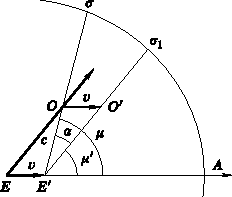
\includegraphics{figure/fig02.09}
    \caption{}
    \label{fig:02.09}
  \end{wrapfigure}
  \example 光行差现象。

  具有不同运动状态的观察者所见的星体的方位是不同的,这
  种差别叫做光行差。因地球公转运动而产生的光行差称为周年光
  行差,因地球自转而产生的光行差称为周日光行差。

  在图\ref{fig:02.09}~中,若观测者相对于某星是静止的,他观测到某星
  在天球上的位置是$\sigma$,则星光到达望远镜物镜中心$O$时,其目镜位
  置在$E'$点。若观测者跟随着地球运动,$EE'$为此时地球的运动方
  向,因星光由$O$点到达目镜的时间为$\tau$,故在此时间内,地球运
  行的距离为$EE'=\tau v$($\vec{v}$为地球运动的速度);因光速为$c$,当星
  光到达目镜时,目镜已移至$E'$点,所以$OE'=\tau c$是星光在$\tau$内传
  播的距离。若地球静止不动,则望远镜对准基的方向为$E'O$。当
  地球运动时,望远镜指向$E'O'$方向才能接收到星光,这是星的视
  方位。相应的,星由真位置$\sigma$移至视位置$\sigma_1$,

  设星的真方位与观测者速度$\vec{v}$间的交角为$\mu$,星的视方位与
$\vec{v}$的夹角为$\mu'$,则光行差为$\alpha$,且有
  \begin{equation*}
    \alpha=\mu-\mu'
  \end{equation*}
  由三角形$OO'E'$,得
  \begin{equation*}
    \frac{\sin\alpha}{\sin\mu'}=\frac{OO'}{OE'}=\frac{\tau v}{\tau c}=\frac{v}{c}
  \end{equation*}

\clearpage
  \begin{equation*}
    \sin\alpha=\frac{v}{c}\sin\mu'
  \end{equation*}
  因为$\alpha$很小,所以
  \begin{align*}
    \alpha & \approx\frac{v}{c}\sin\mu'\text{ 弧度}                                    \\
           & =\frac{v}{c}\sin\mu'\times\frac{180}{\uppi}\times 60 \times 60 \text{ 秒} \\
           & =\frac{v}{c}\sin\mu'\times 206265\text{ 秒}                               \\
           & =k\sin\mu'\text{ 秒}
  \end{align*}
  其中$k$称为光行差常数。

已知地球公转速率为$v=29.770$公里/秒,光速$c=299,774$
公里/秒,所以周年光行差常数
  \begin{equation*}
    k_\text{年}=\frac{29.770}{299,774}\times 206,265=20.48\text{ 秒}
  \end{equation*}

已知地球半径$R=6,378$公里。地球自转一周的时间为$T=
86,164$秒。所以在纬度$\varphi$处的地面速度为
\begin{equation*}
  v_\varphi=\frac{2\uppi R\cos\varphi}{T}=0.464\cos\varphi\text{ 公里/秒}
\end{equation*}
因此,周日光行差常数为
\begin{align*}
  k_\varphi & =\frac{0.464}{299,774}\times 206,265\times\cos\varphi\text{ 秒} \\
            & =0.32\cos\varphi\text{ 秒}
\end{align*}
\section{加速度的相对性}\label{sec:02.04}

根据速度合成公式\eqref{eqn:02.03.06},如果在时刻$t$,质点对于$K$,$K'$
的速度分别为$\vec{v}\left(t\right)$及$\vec{v}'\left(t\right)$,而$K'$相对于$K$以$\vec{u}$作匀速运动,
则有
\vspace{-1.8em}
\begin{equation}\label{eqn:02.04.01}
  \vec{v}'\left(t\right)=\vec{v}\left(t\right)-\vec{u}
\end{equation}
根据加速度的定义。质点相对K的加速度是
\begin{equation}\label{eqn:02.04.02}
  \vec{a}\equiv\frac{\dif \vec{v}}{\dif t}
\end{equation}
而相对于$K'$的加速度是
\begin{equation}\label{eqn:02.04.03}
  \vec{a}'\equiv\frac{\dif \vec{v}'}{\dif t}
\end{equation}
将式\eqref{eqn:02.04.01}对时间求导,得
\begin{equation}
  \frac{\dif \vec{v}'}{\dif t}=\frac{\dif \vec{v}}{\dif t}-\frac{\dif \vec{u}}{\dif t}
\end{equation}
因$ \vec{u} $是不随时间变化的,故$\dfrac{\dif \vec{u}}{\dif t}=0$,所以得
\begin{equation}\label{eqn:02.04.04}
  \vec{a}'=\vec{a}
\end{equation}
这个结果告诉我们,同一质点对于两个相互匀速运动的参考系的
加速度是一样的。换言之,质点的加速度对于相对匀速运动的所
有参考系,具有不变性。

最后指出,对于相对以非匀速运动的两个参考系,式\eqref{eqn:02.04.01}
不再成立。例如,若$K'$相对于$K$作匀加速运动。加速度为$\vec{a}_0$,则
$K'$相对于$K$的速度为$\vec{u}=\vec{a}_0t$,从而式\eqref{eqn:02.04.01}相应改为
\begin{equation*}
  \vec{v}'\left(t\right)=\vec{v}\left(t\right)-\vec{a}_0t
\end{equation*}
由此可以推得
\begin{equation}\label{eqn:02.04.05}
  \vec{a}'=\vec{a} - \vec{a}_0
\end{equation}
这表示对于相对以匀加速度$\vec{a}_0$运动的两个参考系,质点对$K$及$K'$
的加速度$\vec{a}$及$\vec{a'}$,二者之间满足矢量加法关系(式\eqref{eqn:02.04.05}).在这
种情况,加速度是没有不变性或绝对性的。

\section{伽利略变换}\label{sec:02.05}

我们可以把前两节的结果概括如下:对于任何一组相互作匀

\noindent 速运动的参考系而言,速度是相对的,即同一质点相对于不同参
考系有不同的速度;加速度是绝对的,即同一质点相对于不同参
考系的加速度是一样的。

这些结果是相当平凡的,由日常生活的经验也不难接受这些
结果,它们似乎很“浅显”。然而,物理学的特点之一,就是不
放过任何一个“浅显”的概念,总是力图找出这些“浅显”概念
的根基是什么。上两节的目的,正是要找出由式\eqref{eqn:02.03.06}所表达
的速度相对性,和由式\eqref{eqn:02.04.04}所表达的加速度绝对性的根基。

它们的根基就是参考系$K$与$K'$的时空度量之间的变换关系。
现在,我们较仔细地分析一下这个变换关系。

仍假定$K$与$K'$二者相对作匀速运动,$K$的时空坐标为$t$,$\vec{r}$;$K'$
的为$t'$,$\vec{r}'$。$K$与$K'$的时空坐标之间的关系之一,由式\eqref{eqn:02.03.03}给
出,即
\begin{equation}\label{eqn:02.05.01}
  \vec{r}'=\vec{r}-\vec{u} t -\vec{d}_0
\end{equation}
其中$\vec{u}$是$K'$相对于$K$的运动速度。
在推导式\eqref{eqn:02.03.06}或式\eqref{eqn:02.04.04}时,我们还隐含地应用过另外
一个关系。注意在式\eqref{eqn:02.03.05}中我们用了
\begin{equation}\label{eqn:02.05.02}
  \vec{v}'=\frac{\dif \vec{r}'}{\dif t}
\end{equation}
它作为质点相对于$K'$的速度。然而,严格地说,$\vec{v}'$应定义为
\begin{equation}\label{eqn:02.05.03}
  \vec{v}'=\frac{\dif \vec{r}'}{\dif t'}
\end{equation}
即必须用$K'$系的时间$t'$。这样,对比式\eqref{eqn:02.05.02}及式\eqref{eqn:02.05.03}就可
以看到,在这里我们实质上假定$\dif t'=\dif t$,或者
\begin{equation}\label{eqn:02.05.04}
  t'=t+t_0
\end{equation}
其中,$t_0$为一常数。

式\eqref{eqn:02.05.01}及式\eqref{eqn:02.05.04}给出了$K$与$K'$的时空坐标之间的完整
的变换关系,它被称为伽利略变换。式\eqref{eqn:02.03.06}及式\eqref{eqn:02.04.04}都只是伽利略变换的推论。

伽利略变换表明,时间、空间具有下列的基本性质。

\heiti 1. 时间间隔的绝对性 \normalfont

对于一个运动过程,相对于$K$,它的开始与终了的时刻若分
别为$t_1,t_2$,则相对于$K'$它的开始与终了的时刻分别为$t_1'=t_1+t_0,t_2'=t_2+t_0$,因此有
\begin{equation}\label{eqn:02.05.05}
  \Delta t \equiv t_2 - t_1 = t_2' - t_1' \equiv \Delta t'
\end{equation}
上式的物理意义是,一个过程的时间间隔与参考系的选取无关,
是绝对的。

\heiti 2. 长度的绝对性 \normalfont

有任一直尺,相对于$K$,它的两个端点的坐标为$\vec{r}_1,\vec{r}_2$,则相
对于$K'$,端点的坐标应分别是$\vec{r}_1' = \vec{r}_1 - \vec{u} t - \vec{d}_0,\vec{r}_2' = \vec{r}_2 - \vec{u} t - \vec{d}_0$,
故有
\begin{equation}\label{eqn:02.05.06}
  |\vec{r}_1 - \vec{r}_2| = |\vec{r}'_1 - \vec{r}'_2|
\end{equation}
它的物理意义是,一直尺的长度是与参考系的选取无关的,是绝
对的。

总之,速度相对性是以时间间隔和长度的绝对性为基础的。

\section{速度合成律的失效}\label{sec:02.06}

如图\ref{fig:02.10}~所示,如果在炮车上装有两门相同的大炮,一门向
右,一门向左。如果炮车相对地面静止\lbr 图\ref{fig:02.10a}\rbr,这时,不论
从地面参考系$K$,还是从炮车参考系$K'$看,同时向左、右发射出
的炮弹的速率都是$v$。如果炮车相对地面以$u$的速率向右匀速运动
\lbr 图\ref{fig:02.10b}\,\rbr ,从$K$看,按速度合成规律\lbr 式\eqref{eqn:02.03.06}\,\rbr ,向右的炮
弹速率是$v+u$;向左的炮弹速率是$v-u$。实验也相当精确地证
明了这一点,它表明,速度的合成公式是符合实际的。

我们现在要问:速度合成律对任何情况都成立吗?

\clearpage
\begin{figure}
  \centering
  \subfigure[]{
    \includegraphics{figure/fig02.10a}
    \label{fig:02.10a}
  }
  \hspace{2em}
  \subfigure[]{
    \centering
    \includegraphics{figure/fig02.10b}
    \label{fig:02.10b}
  }
  \caption{速度的合成}
  \label{fig:02.10}
\end{figure}

\begin{figure}
  \centering
  \includegraphics{figure/fig02.11}
  \caption{光的速度合成}
  \label{fig:02.11}
\end{figure}

再考虑一个如图\ref{fig:02.11}~所示的实验,这里仅把大炮改为灯泡,
灯泡发出的光与炮弹相当,光相对于灯泡的速率是$c$。根据速度合
成律,当灯泡相对于地面以速率$u$向右匀速运动时,则向右发出的
光对于地面参考系$K$的速率应是$c+u$,而向左发出的光对于$K$的
速率应是$c-u$。这个结果对吗?现在我们举一些显而易见的例
子,来说明这个结果是不正确的。

上述实验是把速度合成律应用到光传播的现象中去。根据光
学知识,我们知道,一个物体$A$之所以能被看到,是由于从物体
$A$发出的光(或从它反射的光)传到了我们的眼睛。例如,在图\ref{fig:02.12}~
中,1投球,2接球。2看到球$A$,是由于球$A$发出的光到达2。如果
光速为$c$,1到2之间距离为$L$,并且1即将投球的时刻为$t=0$,则
2看到1即将投球的时刻为
\begin{equation*}
  t_{2\text{投}}=\frac{L}{c}
\end{equation*}
\begin{figure}
  \centering
  \includegraphics{figure/fig02.12}
  \caption{光的速度合成引起的混乱}
  \label{fig:02.12}
\end{figure}%
当1刚刚将球投出时,球$A$速率为$u$,如果光也满足速度合成律,
那么,这时球$A$发出的光相对于地面的速度应为$c+u$。如果1刚
刚将球投出的时刻是$t=t_{1\text{出}}$(即1投球这一动作所用的时间间隔),
则2看到1刚刚将球投出的时刻应为
\begin{equation*}
  t_{2\text{出}} = t_{1\text{出}} + \frac{L}{c+u}
\end{equation*}

从原则上讲。我们总有办法(譬如增大$L$)使下式成立
\begin{equation*}
  \frac{L}{c} > t_{1\text{出}} + \frac{L}{c+u}
\end{equation*}
亦即
\begin{equation*}
  t_{2\text{投}} > t_{2\text{出}}
\end{equation*}
上式表明,2看到1开始投球的时刻比他看到1已经投出球的时刻
还要晚。更形象地说。2将先看到球$A$飞出,而后才看到1的投球
动作。这就是说,如果光的传播也满足速度合成公式\eqref{eqn:02.03.06},必然
导致先看到后发生的事,后看到先发生的事这种奇怪的现象,然
而,谁也没有见过这种现象。这说明光并不满足速度合成公式。

当然,有人会说,上述例子是假想实验,由于光速是很大
的,$L/c$或$L/\left(c+u\right)$实际上都接近于零,因而不可能观测到这种
现象。的确,在日常生活中涉及的速度与光速相比都是很小的,
把光速看成无限大,上述矛盾就没有了。但是,光速并不总能被
看成无限大,特别是在天体尺度上,光速不能被认为是无限大,光
传播中的矛盾是逃避不掉的。下面我们分析一个天文学上的真实
例子。

我国史书《宋史》中有下列的记载:“至和元年五月己丑出
天关东南可数寸岁余稍没”,《宋会要辑稿》也记载:“至和元
年五月晨出东方守天关昼见如太白芒角四出色赤白凡见二十三
日”。这个重要的天文观测记录说的是一次非常著名的超新星爆
发事件,现称为公元1054年的超新星。

所谓超新星指的是恒星在特定的演化阶段出现的一次大爆
发。原来发光很弱的星体,在爆发时,向外抛出速率很高的大量
物质,并发出很强的光,过不长的一段时间,又再暗下去。现在
巳确定,1054年超新星的遗迹就是金牛座中的蟹状星云,它到地
球的距离约为$L \approx 5000$光年,爆发时,喷射物的速率至少有
$u=1500$公里/秒。
\vspace{1em}
\begin{figure}[h]
  \centering
  \includegraphics{figure/fig02.13}
  \caption{超新星爆发过程中光的传播}
  \label{fig:02.13}
\end{figure}

由图\ref{fig:02.13}~看出,如果爆发时刻为$t=0$,且爆发时间极短,则
根据速度合成律,1处发出的传向观察者的光相对地面的速率是
$c+u$,所以观察者看到l发光的时刻是

\begin{equation*}
  t_{1}=\frac{L}{c+u} \approx \frac{L}{c}\left(1-\frac{u}{c}\right)
\end{equation*}
同样,根据速度合成律,2处(弧$\wideparen{12}=\ang{90;;}$)发出的传向观察者的光
相对于地面的速率约为$\sqrt{c^2 + u^2}$,故观察者看到2发光的时刻是
\begin{equation*}
  t_{2}=\frac{L}{\sqrt{c^{2}+u^{2}}} \approx \frac{L}{c}\left(1-\frac{1}{2} \cdot \frac{u^{2}}{c^{2}}\right)
\end{equation*}
显然,观察者见弧$\wideparen{12}$中发光的时刻介于$t_1$到$t_2$之间,因此观察者
看到星发光的时间至少应是
\begin{equation*}
  \Delta t=t_{2}-t_{1} \approx \frac{Lu}{c^{2}}
\end{equation*}
代入有关数据,计算而得
\begin{equation*}
  \Delta t=25\text{年}
\end{equation*}

如果爆发不作瞬时过程处理,则看到超新星的时间应比25年
还要长。

但是,这个下限与实际观测是不相符合的。记录上说:“凡
见二十三日”(白天看到)或“岁余稍没”(夜里看到)。即一年多
就消没了。

上述真实例子说明,对于光传播的现象,速度合成律是失效
的。它说明,从超新星不同地方发出的光,即不同光源发出的光,
相对于地面的速率之间的差别,不应有式\eqref{eqn:02.03.06}~所给出的那样
大。现代更精确的实验表明。光速是与光源速度无关的,无论光
源的速度有多么大,由它发出的光的速度仍与静止光源发出的光
的速度相同。这就是光速不变性,这个特点最初是由爱因斯坦注
意到的。

显然,光速不变性与速度合成律\lbr 式\eqref{eqn:02.03.06}\,\rbr 之间存在着严重
的矛盾,而问题的根源就在于伽利略变换并不总是适用的。
\section{光速不变的结论之一——运动钟的变慢}\label{sec:02.07}

现在我们来分析,从光速不变性能得出什么结论。光速不变
性使我们所看到的物理现象总是因果相继的,免除了因果倒置的
混乱。但是,光速不变性却动摇了另一个传统观念一时间间隔
的不变性。

我们可以用光速不变性来设计一种雷达钟。图\ref{fig:02.14a}~是一
个雷达式的装置,在距离雷达天线$d$处放一反射镜,那么,从天
线发出光信号到天线重又接收到这个光信号一个来回的时间间隔
应为
\begin{equation*}
  \Delta t ' = \frac { 2 d } { c }
\end{equation*}
\begin{figure}[!h]
  \centering
  \subfigure[]{
    \label{fig:02.14a}
    \includegraphics{figure/fig02.14a}
  }
  \quad
  \subfigure[]{
    \label{fig:02.14b}
    \includegraphics{figure/fig02.14b}
  }
  \caption{雷达钟}
  \label{fig:02.14}
\end{figure}

由于光速不变,我们可以用一个来回作为度量时间的单位。这个
装置就是一种钟。

现在,我们让这个钟固定在$K'$中,一起以匀速$u$相对于K沿
垂直于$d$的方向运动。在$K'$中看,光信号一个来回仍走$2d$,它的
时间间隔仍为
\begin{equation*}
  \Delta t ' = \frac { 2 d } { c }
\end{equation*}
% 079.jpg
但是在$K$中看来,光信号这时走的是之字形路径〔图\ref{fig:02.14b}〕光
信号发出时,钟位于1,镜反射光信号时,位于2,接收光信号时,
位于3。因而,这光信号的一个来回,在$K$中看来是走两条斜线。
如果这个来回在$K$中看,所需时间间隔为$\Delta t$,则按光速不变性,
斜边长为$\dfrac { 1 } { 2 } c \Delta t $ ,底边1到2的长$\frac { 1 } { 2 } u \Delta t$ ,故由直角三角形关系
有
\begin{align*}
  \left( \frac { 1 } { 2 } c \Delta t \right) ^ { 2 } & = \left( \frac { 1 } { 2 } u \Delta t \right) ^ { 2 } + d ^ { 2 }                                             \\
                                                      & = \left( \frac { 1 } { 2 } u \Delta t \right) ^ { 2 } + \left( \frac { 1 } { 2 } c \Delta t ' \right) ^ { 2 }
\end{align*}
解之得
\begin{equation}\label{eqn:02.07.01}
  \Delta t = \frac { \Delta t ' } { \sqrt { 1 - \dfrac { u ^ 2 } { c ^ { 2 } } } }
\end{equation}

此式表明,在$K'$中需用$\Delta t '$时间间隔的过程,在$K$中观测就
不等于$\Delta t$,而是$\Delta t > \Delta t '$ 。当$K'$中的钟走了一个单位时间间隔
即$ \Delta t ' = 1 $时,$K$中的钟已走了
$\dfrac { 1 } { \sqrt { 1 - \dfrac { u ^ 2 } { c ^ { 2 } } } } > 1$。也就是说,由$K$看
来,$K'$中的钟变慢了。$K$看$K'$的钟是在运动,故运动的钟变慢。
反过来,由$K'$来看$K$中的钟时,我们可以用完全相同的推理
方法(注意此时$K$沿$K'$的$x'$的负向以速率作匀速运动),得到
\begin{equation}\label{eqn:02.07.02}
  \Delta t ' = \dfrac { \Delta t } { \sqrt { 1 - \dfrac { u ^ 2 } { c ^ { 2 } } } }
\end{equation}
可见,$K'$看$K$中的钟也变慢。

有人会说,这岂不矛盾!其实并不矛盾。因为他们是在不同
的“立场”上说话的,两种说法实际上是一致的,可以统一地表
% 080.jpg
达为: \CJKunderdot{相对于观测者运动的钟变慢}。

\clearpage
时间的变慢已有大量的实验证明。最有名的是$\mu$子的衰变。
从实验室中产生的$\mu$子,寿命只有约~$\num{2.2e-6}$~秒,这样,即使它
以光速$ c \approx \num{3e8} $米/秒运动,也只能走过
\begin{equation*}
  \num{2.2 e -6} \times \num{3e8} = 660 \text{ 米}
\end{equation*}

另一方面,宇宙射线产生子的区域约在$1500\sim2000$米的高
空。但是我们发现不少从上层大气中产生的从子跑到地面上来了。
为什么?就因为寿命~\num{2.2 e -6}~秒是对于$\mu$子静止的参考系$K'$而
言的,当$\mu$子运动时,在地面上(即参考系$K$)看来,它的寿命应为
$\Delta t = \dfrac { \num{2.2e-6}}{ \sqrt { 1 - \dfrac { u ^ 2 } { c ^ { 2 } } } }$
秒,其中$u$是$\mu$子的运动速度,当$u$接近于$c$
时,$\Delta t$比~\num{2.2e-6}~秒大得多,即$\mu$子的寿命变长了,因而它可以
飞过距离
\begin{equation*}
  L = u \Delta t \gg 660 \text{ 米}
\end{equation*}
即能从高空飞到地面上来。

1964年,欧洲核子研究中心(CERN)通过实验定量地验证了
时间延长公式。用两个同时产生的$\mu$子,让其中之一相对于实验室
静止,另一个在加速器中运动。结果证明,运动子的寿命变长,
两子的寿命比值和在加速器中的运动速度$u$之间的关系完全符合
式\eqref{eqn:02.07.02}。

运动钟变慢与我们从日常生活中得来的感觉完全不同。因此,
不免有人会问:“到底钟是否真的变慢了?”物理学,特别是力
学,有很多内容是描写我们日常看到和感觉到的东西的。但是,
物理学与我们日常的直观有很多不同。物理学要求每个陈述有明
确的含义,特别是要指出每一个物理量是如何测量的,然后再在
这个基础上研究规律的建立。一般地诉诸于感觉如何如何,这不
是物理学,只不过是粗浅的认识。
% 081.jpg

\clearpage
上述的“到底”一问似乎很有道理,但却是没有物理价值的,
为什么?因为该处的“到底”是不能测量的。如果能指出“到底”
是在什么情况下进行什么测量的,我们才可作出明确的回答。如
果不能指出这一点,那说明这个问题本身就是非物理的,物理学
不研究这类问题。一旦研究测量方法,而测量又要相对于一定的
参考系,则必然走到我们上述的体系中去。

物理学的基础是测量,如果在原则上含有不能测量的东西,
这种东西本身就缺乏物理意义,因为这种不能测量的东西,既无
法用实验证实它,也无法否证它。用现代物理学的语言说,一种
理论要具有物理价值,就要具有可证伪性,即所有有关的量以及
断言,都能直接或间接由实验加以验证。这是我们判断一种理论
有没有物理价值的基本原则之一。

\section{光速不变的结论之二——运动尺的变短}\label{sec:02.08}

在上节中,我们看到光速不变动摇了伽利略变换的根基之
一——时间间隔的绝对性。现在我们将证明,在光速不变的前提
下,伽利略变换的另一个根基一长度的绝对性也不再成立。

对地面上的观测者来说,从大气层上部冲下来的$ \mu $子的寿命
延长了。随同$ \mu $子一起运动的观测者会看到什么情况呢?

由于相对于子为静止的观测者与地面上的观测者都同样观
测到$ \mu $子从高空运动到地面这一事实,而且他们也都观测到他
们之间的相对速度是$u$。对于地面上的观测者来说$\mu$子的寿命$\Delta t = \dfrac{\num{2.2e-6}}{\sqrt{1 - \dfrac{u ^ 2}{c ^ 2}}}$
秒,$\Delta t$大了,故$ L \left( = u \Delta t \right)$大于$\mu$子出生处到地面的
高度,所以它能到达地面。而随$\mu$子运动的观察者所看到$\mu$子的寿
命应是~\num{2.2e-6}秒。那么他怎么解释$\mu$子到达地面这一事实呢?
% 082.jpg
这只能有一种可能性,即随同$\mu$子运动的观测者主张:$\mu$子出生
处到地面的距离变短了。即一旦时间间隔不变性不成立,则长度
不变性也要被破坏。如果我们设想从地面到高空立着一个尺,尺
静止在地面上,地面观察者看尺长为$L$;而相对于$\mu$子静止的观
察者看来,这尺长为$L'$,即
\begin{equation*}
  \frac { L } { \Delta t } = \frac { L ' } { \Delta t ' }
\end{equation*}
\begin{equation}\label{eqn:02.08.01}
  L ' = L \frac { \Delta t ' } { \Delta t } = L \sqrt { 1 - \frac { u ^ { 2 } } { c ^ { 2 } } }
\end{equation}
这尺对于$\mu$子上的观察者在运动,故$ L ' < L $,即运动的尺变短。

\begin{figure}[!b]
  \centering
  \subfigure[静止的雷达钟]{
    \label{fig:02.15a}
    \includegraphics{figure/fig02.15a}
  } \\ \vspace{-0.3em}
  \subfigure[运动的雷达钟]{
    \label{fig:02.15b}
    \includegraphics{figure/fig02.15b}
  } \\ \vspace{-0.3em}
  \subfigure[光信号向右传播]{
    \label{fig:02.15c}
    \includegraphics{figure/fig02.15c}
  } \\ \vspace{-0.3em}
  \subfigure[光信号向左传播]{
    \label{fig:02.15d}
    \includegraphics{figure/fig02.15d}
  }
  \caption{}
  \label{fig:02.15}
\end{figure}
现在我们来证明式\eqref{eqn:02.08.01}。我们仍使用一个雷达钟。如
图\ref{fig:02.15a}\\所示,当雷达钟与地面相对静止时,从地面参考系,即$K$
% 083.jpg
系来观察,它的天线与反射面之间的距离为$ d$;当雷达钟以速度
运动时\lbr 图\ref{fig:02.15b}\rbr ,由$K$系测得的距离表示为$d'$。

我们考察光信号来回一次的运动。由于光在传播过程中雷达
在不断地运动,所以,由$K$看来,光传播的距离并不是$d'$。例如,
当光向右传播,从天线到达反射面时,若所用的时间为$\left(\Delta t\right)_1$,则
所走过的距离应为$ d ' + u \left( \Delta t \right) _ { 1 }$,其中$ u \left( \Delta t\right) _ { 1 } $一项表示在$\left(\Delta t\right)_1$时
间中钟向右运动的距离\lbr 图\ref{fig:02.15c}\rbr 。这样,我们有
\begin{equation*}
  \left( \Delta t \right) _ { 1 } = \frac { d ' + u \left(\Delta t\right)_1 } { c }
\end{equation*}
或者
\begin{equation}\label{eqn:02.08.02}
  \left( \Delta t \right) _ { 1 } = \frac { d ' } { c - u }
\end{equation}
类似地,光从反射面到天线的传播过程所用的时间$ \left(\Delta t\right)_2 $应是
\begin{equation}\label{eqn:02.08.03}
  \left( \Delta t \right) _ { 2 } = \frac { d ' } { c + u }
\end{equation}
由式\eqref{eqn:02.08.02}及式\eqref{eqn:02.08.03}可以得到光信号一个来回耗费的时间
\begin{equation}\label{eqn:02.08.04}
  \Delta t = \left( \Delta t \right) _ { 1 } + \left( \Delta t \right) _ { 2 } = \frac { 2 c d ' } { c ^ { 2 } - u ^ { 2 } }
\end{equation}
这是$K$系看到的结果。

在$K'$系,即雷达钟参考系来看,这个过程仍由下式描写
\begin{equation*}
  \left( \Delta t \right) ' = \frac { 2 d } { c }
\end{equation*}
因为在$K'$系观察,钟的长度是$d$。这样,式\eqref{eqn:02.08.04}可以改写为
\begin{equation*}
  \Delta t = \frac { 1 } { 1 - \dfrac { u ^ { 2 } } { c ^ { 2 } } } \left ( \frac { d ' } { d } \right) \left( \Delta t \right) '
\end{equation*}
再由上节推知的时间关系式\eqref{eqn:02.07.01},上式就成为
\begin{equation*}
  d ' = d \sqrt { 1 - \frac { u ^ { 2 } } { c ^ { 2 } } }
\end{equation*}
% 084.jpg
\clearpage
\noindent 这就是式\eqref{eqn:02.08.01}

本节和上节的讨论用的都是雷达钟,因此,就存在一个共同
的问题,即运动钟的变慢和运动尺的变短是否普遍?或者,这些
推论是否只反映了雷达钟本身的性质,如果选择其他的钟有没有
这种性质?这些问题我们留待第十一章再来讨论

\begin{questions}

  \question 在亚里士多德体系中,哪些物理量是绝对的?哪些物理量
  是相对的?在牛顿体系中,哪些物理量是绝对的?哪些物理量是
  相对的?

  \question 变换关系式\eqref{eqn:02.03.06}是否只适用于$u$为常量的两个坐标间
  的速度变换?

  \question 试再举出一些有用的坐标变换。

  \question 试举出一种相对于时间倒转变换为不变的运动。

  \begin{wrapfigure}[10]{r}{12em}
    \includegraphics{figure/fig02.16}
    \caption{}
    \label{fig:02.16}
  \end{wrapfigure}

  \question 双星是一种天体,两颗星
  绕它们共同的质心在一封闭的轨
  道上绕行(图\ref{fig:02.16}),如果我们的
  视线在轨道平面上,则双星中任
  何一颗星有时向着我们运动,有
  时离开我们运动。假使光速与光
  源速度有关,可用速度合成公式
  \eqref{eqn:02.03.06}。这样,我们将会看到什
  么现象?

  \question 如果地球总是以恒定的
  速度运动,也没有自转,能探测到光行差效应吗?

  \question 由于地球的周年运动引起的光行差效应,使得恒星的视位
  置在一年之中绘出怎样的图形?
  % 085.jpg
  \clearpage
  \question 在\ref{sec:02.07}~节中所述“运动钟的变慢”,是否是由于我们选用的雷达钟的特殊结构而引起的?
\end{questions}

\begin{exercises}

\exercise 以不同的速率同时向不同方向抛出两物体。证明在运动的
时候,若不计空气阻力,它们的相对速度固定不变。

\exercise 有一水平飞行的飞机,速度为$ v _ { 0 }$,在飞机上安置一门炮,炮弹以水平速度$ v $向前射击。略去空气阻力,求

(1) 以地球为参考系时炮弹的轨迹

(2) 以飞机为参考系时炮弹的轨迹

(3) 以炮弹为参考系时飞机的轨迹

\exercise 一辆汽车尾部敞开,顶篷只盖到$A$处(图\ref{fig:02.17}),乘客可坐
\begin{wrapfigure}[7]{r}{13em}
  \includegraphics{figure/fig02.17}
  \caption{}
  \label{fig:02.17}
\end{wrapfigure}
到车尾$B$处,$AB$联线与铅直方向
成$ \varphi = 3 0 ^ { \circ }  $角。汽车在平直公路上
冒雨行驶,当其速率为6公里/时
时,$C$点刚好不被雨打着若它
的速率为18公里/时,则$B$点就
刚好不被雨点打着。求雨点的速
度$ \vec{v} $。

\exercise 以速率$ v _ { 1 }  $运动的列车上的驾驶员,发现在前面与该车相距
$d$处,有一列车在同一轨道上沿相同方向、以较小的速率$v_2$在运
动,他立刻用制动器刹车,使他的火车以匀减速$a$慢下来,试证
明:

(1) 如果$d > \dfrac { \left( v _ { 1 } - v _ { 2 } \right) ^ { 2 } } { 2 a }$
则两车不会相撞;

(2) 如果$d < \dfrac { \left( v _ { 1 } - v _ { 2 } \right) ^ { 2 } } { 2 a }$
,则两车将要相撞。
% 086.jpg

\clearpage
\exercise 渔人在河中乘舟逆流航行,经过某桥下时,一只水桶落入
水中,半小时后他才发觉,即回头追赶,在桥的下游5.0公里处赶
上。设渔人顺流及逆流相对水的划行速率不变,求水流速率。

\exercise 甲乙两列火车在相邻的轨道上相向运行,甲的速率为$v_1$,
乙的速率为$v_2$。从甲车上水平地投一物到乙车上。设投掷速率为
$v _ { 0 }$ ( $v_0  $在物体运动的全部时间内可认为是不变的),从甲车上看,投
掷方向与列车行驶方向垂直,试求:

(1)物体的轨迹在路基上的投影与铁轨所成的角$ \varphi _1 $;

(2)物体的轨迹在乙车上的投影与乙车边缘所成的角$ \varphi _2 $;

(3)物体相对于路基的速度$ v' $和相对于乙车的速度$ v'' $。

\exercise 飞机罗盘指示飞机正在朝东飞行,地面情报指出,
此时刮着正南风。如果风速$ | \vec{u} | = 4 0 . 0  $公里/时,飞机相对空气的
速度为$ | \vec{v} ' | = 2 0 0  $公里/时,试用矢量图表明:飞机相对于地面的
速度$\vec{v}$;驾驶员应怎样驾驶才使其前进方向相对于地面是朝向正
东?

\exercise 一架飞机以相对于空气的匀速率$u$作水平直线飞行,从$A$飞
到$B$再返回,从$A$到$B$的距离是$L$。如果速率为$v$的风向有下列三
种情况(都有$ u > v$)  :

(1)沿着从$A$到$B$的直线

(2)垂直于从$A$到$B$的直线

(3)与$A$到$B$的直线成角。\\
试求往返一次所需要的时间。并证明,由于风的存在,往返时间
总是比无风的情况长。

\exercise 一升降机以$ a = 2 g  $的加速度从静止开始上升,在2.0秒末时
有一小钉从顶板下落,若升降机顶板到底板的距离$ k = 2 . 0  $米,求
钉子从顶板落到底板的时间$t$,它与参考系的选取有无关系?

\exercise 一飞机在海上布雷,当它在水面上高为$h$的地方以速率$v$
沿水平方向飞行时,要想使鱼雷入水时,鱼雷不与水面发生拍击,
即相对于鱼来说,水的速度完全沿鱼雷的轴线方向(图\ref{fig:02.18})。
% 087.jpg
\begin{wrapfigure}[8]{r}{15em}
  \includegraphics{figure/fig02.18}
  \caption{}
  \label{fig:02.18}
\end{wrapfigure}
设鱼雷从投下到入水,它的轴线与水平面的
夹角不变。略去空气阻力,求当飞机投射鱼雷时,$\theta$应
当等于多少?

\exercise 设某一超新星到地
球的距离$ L \geqslant 1 0 ^ { 6 }  $光年,若爆发是匀速球状膨胀,膨胀速率$|\vec{v}|$约为$5 \times 1 0 ^ { - 3 }  $光年/年。如果光速与光源速度有关,爆发后,在地球上
有多长时间间隔都能观测到它的最大光度?

\exercise 在某一参考系$K$看来,物体$A$以匀速率$v_A$沿$x$轴正向运动,
物体$B$以匀速率$v_B$沿$x$轴的负方向运动。试问:

(1) 在参考系$K$看来,\!$A$与$B$之间相对运动的速度$v_{A\!B}$是多大?

(2) $c$为真空中的光速,当$ v _ { A }$=0.8$ c $,\!$ v _ { B }$=0.6$ c  $\,时,\!$v_{A\!B}$是多少?

(3) 在同一参考系$K$中看来,两个物体$A$与$B$之间相对运动的
速度$ v _ { A B } > c  $,是否违反狭义相对论?为什么?

(4) 在$A$看来(即在随$A$一起运动的坐标系$K'$里看),$B$的速
度$ v _ B ' $仍旧是$v_{AB}$吗?

\exercise~ $K$和$K'$是两个相互平行的系,$K'$相对于$K$沿$x$轴以的$\dfrac { 1 } { 2 } c $速率运动。问:

(1) 在$K$系中静止放置一把尺子,长为$l$,在$K'$系来测量,尺
子的长度是多少?

(2) 在$K$系中某点$A$发生一事件,时间间隔为$\Delta t$,在$K'$系来
看,这事件的时间间隔是多少?

\exercise 在实验室中观测到一个运动着的$\mu$子在实验室坐标系中
的寿命等于静止$\mu$子寿命的50倍,求$\mu$子相对于实验室坐标系
运动
% 088.jpg
的速度$v$。

\clearpage
\exercise 爱因斯坦在他的创立狭义相对论的论文中说:“一只在
地球赤道上的钟,比放在两极的一只在性能上完全一样的钟,在
别的条件都相同的情况下,要走得慢些。”根据各种观测,地球
从形成到现在约为50亿年。假定地球形成时,就有爱因斯坦所说
的那两只钟,问:现在它们所指示的时间相差多少?已知地球半
径为6378公里。

\exercise 按上题同样道理,在地球看来,一只在月球上的钟,要比
一个性质完全相同,所处条件也完全相同,放在地球上的钟走得
略为慢些。设地球年龄为$ \tau = 5 0  $亿年,月球绕地球转动的平均速率
为$ v = 1 . 0 2 \times 1 0 ^ { 5 }  $厘米/秒。月球上的钟在50亿年里比地球上的钟慢了多少?

\exercise 类似15题,在太阳上的观测者将看到一只在地球上的钟,
要比一只性能完全相同、所处条件也完全相同放在太阳上的钟走
得略为慢些。设太阳年龄为$ \tau = 5 0  $亿年,已知地球公转的平均速率
为$ v = 2 9 . 7 6  $公里/秒。地球上的钟在50亿年里比太阳上的钟慢了
多少?

\exercise 一个“光钟”由两个相距为$ L _ { 0 }  $的平面镜$A$和$B$组成。对于
这个光钟为静止的参考系来说,一个“滴答”的时间是光从镜面
$A$到镜面$B$再回到原处的时间,其值是$ t _ { 0 } = 2 L _ { 0 }  /c$。若将这个光钟横
放在一个以速度$\vec{v}$行驶的火车上,使两镜面都与$\vec{v}$垂直,而两镜
面中心联线则与$\vec{v}$平行。这时,若在铁轨参考系中看,火车上钟
的一个“滴答”$\tau$与$\tau _ 0$的关系怎样?

\exercise ~ $\mu$子是不稳定的粒子,它自发地衰变为
\begin{equation*}
    \mu ^ \pm \longrightarrow e ^ \pm + \overline{\nu} _ { e } + \nu _ { \mu }
\end{equation*}
其中$\mu ^ \pm$分别表示带正电或带负电的$\mu$子,$\overline{\nu} _ { e }$表示反中微子,
$\nu _ { \mu}$表示$\mu$中微子。上述自发衰变的寿命是
$ \tau _ { 0 }$=2.2$\times$10$^{-6}$秒,这是对$\mu$子静
止的坐标系而言的。若$\mu$子的速度$ v$=0.995$c$,它的寿命将为多少?
\end{exercises}




% 第三章
\chapter{牛顿动力学}\label{chp:03}

\section[惯性定律]{\makebox[5em][s]{惯性定律}}\label{sec:03.01}

在上两章中,讨论了运动的描述,而没有涉及运动的原因,
没有研究不同式样的运动之间的内在联系。譬如,自由落体为什
么垂直向下做匀加速运动?行星为什么绕太阳旋转不息?自由落
体与行星旋转两者之间有什么关系?这些就是本章及随后几章要
讨论的问题。

研究物体运动的原因,通常称之为动力学。牛顿动力学就是
有关物体的机械运动的动力学。可以说整个物理学的基本规律就
是各种运动形态的动力学的总合。

牛顿动力学中的核心概念是力。

经验告诉我们,物体的运动是由物体之间的相互作用引起的。
列车的行进是由于机车的牵引作用,枪弹的射击是靠着炸药爆炸
的作用。物体之间的相互作用,用“力”这个概念来表达。实际
上,人对力最初的认识是源于人的肌肉对外物的作用。汉字的力,
在篆书中的写法,就是筋肉的象形。

力的概念虽然出现得很早,但是关于力和运动的关系的正确
认识,却得到得相当晚。在亚里士多德的《物理学》中有一条原
理:“凡运动着的事物必然都有推动者在推动着它运动。”这个
论断在几乎两千年的时间里,被认为是无可怀疑的经典。的确,
% 090.jpg
我们日常看到的各种运动似乎都遵从这个论断,即必定有推动者
(即力)在维持着它的运动。就象一定的踏力保持着自行车的一定
的运动状态,而一当踏力消失,车最终要变成静止。

\begin{wrapfigure}[7]{r}{16.5em}
  \includegraphics{figure/fig03.01}
  \caption{伽利略的斜面}
  \label{fig:03.01}
\end{wrapfigure}
伽利略开始明确地认识到亚里士多德的经典是不完全正确的,尽
管许多运动的确都要靠外力的维持,但并非凡运动皆如此。伽利略用
一个理想实验来证明亚里士多德的错误。他研究斜面上的运动(图\ref{fig:03.01}),
让一小球从斜面
上滚下。已经知道,小球的下滚是由于重力的作用,重力沿着斜面
的分量拉着小球下滚。如果高度不变,$\alpha$越小,则$ L $越大,同时
重力沿斜面的分量也越小。伽利略曾做过一系列小球沿斜面下滑
的实验。他发现,只要斜面足够光滑,无论$\alpha$多么小,小球总能
从斜面上滚下来。由这个结果就可以推测,即使当$ a \rightarrow 0$  ,$L \rightarrow \infty$
的情况,小球还是可以滚“下”来的。显然,对$ a \rightarrow 0$  ,$L \rightarrow \infty$情
况是无法直接做实验的,但从已知的实验结果可以推知这种极限
情况的现象。这就是理想实验方法的关键。

在$ a \rightarrow 0$  ,$L \rightarrow \infty$情况,重力沿斜面的分量为零,即并没有外
力推动小球“下”滚。因此,这种运动就是一种没有“推动者”
的运动。对亚里士多德的“凡运动必有推动者”来说,上述运动
就是一个反例。

伽利略的分析弄清了,存在一类运动,它们并不是由外力所
维持。它们的特征是速度保持不变,即作匀速率的直线运动,或
者静止。我们称物体不受外力作用的运动状态为自由运动。总之,
处在自由运动状态的物体,必定作匀速直线运动,或者静止。这
就是惯性定律。
% 091.jpg

有人可能会想到,速度或加速度都是具有相对性的,对参考
系$K$为匀速运动的物体,在参考系$K'$中可能成为非匀速的。那么,
一个自由运动的物体,在有些参考系看来不也是作着非匀速运动
吗?的确,在某参考系看来,一个不受力的物体也会作非匀速运
动。

然而,惯性定律的意义是在于断言:对于一个物体的自由运
动,一定可以选择一个参考系$K$,相对于$K$该物体作匀速运动或
静止,而且,其他所有自由运动的物体,对于$K$来说,也都是作
匀速运动或静止。换言之,一定存在着这样的参考系,相对于
它,所有不受外力作用的物体都保持自己的速度。这类特殊的参
考系,称为惯性参考系,或惯性系。

简言之,惯性定律就是断定了惯性系一定存在。

惯性定律的确立,成为旧物理学(即亚里士多德物理学)的终
点,同时也成为新的力学的起点。常称惯性定律为牛顿第一定律。
本章以后的讨论,都采用惯性系。
\section{牛顿第二定律}\label{sec:03.02}

牛顿第一定律确立了不受力情况下物体的运动性质。本节讨
论牛顿第二定律,它确立了外力对物体运动的作用。这个定律是:
如果一个质点受到外界物体的作用,则它的运动遵循下列关系:
\begin{equation}\label{eqn:03.02.01}
  \vec{F} = m \vec{a}
\end{equation}
其中$\vec{a}$是质点的加速度,$m$是它的质量;$\vec{F}$是外物对它的作用力。

在此定律中,我们一下子涉及了两个新的物理量:$m$及$\vec{F}$。虽然
在上节讨论过力,但只限于受力或不受力,并没有给出力的定量的
定义,以及如何从动力学的角度来定义力。另一方面,质量的粗浅
概念也早就有了,问题同样是:什么是质量?并未解决。也曾有过各
式各样的有关质量的定义。例如,有的定义是:质量是物体所含
% 092.jpg
“物质的量”然而,这种定义没有物理的价值。因为,什么叫“物质
的量”?仍然是不确定的。在物理学中,一个物理量的定义,必
须提供根据其他能够量度的量来计算它的一套规则。根据这个原
则,在牛顿第二定律的范围中,可以对质量及力作如下的定义:

质量就是质点所受外力与所产生的加速度之比。

作用在一个质点上的力就是它的质量乘由于该力所产生的加
速度。

看到这两条“定义”,读者一定会纳闷,这两条说法岂不就
是式\eqref{eqn:03.02.01}的改头换面吗?这样一来,作为定律的式\eqref{eqn:03.02.01}岂
不降为关于质量或力的定义?似乎出现了逻辑上的“混乱”。

如果离开上述的物理定义的原则,确实总逃不脱这个“混
乱”。但是,从物理上来说,它是不混乱的。物理规律的作用在
于把许多已知的实验结果统一起来,联系起来,给出许多实验现
象的统一的解释,并且根据这种解释去预测一些新的现象或实验
结果。也就是说,物理学规律的意义,是使我们能够从一些实验结
果出发预言另一些新的实验结果,确立从一些实验数据计算出(或
预言出)另一些实验数据的规则。只要定义、定律确立的联系测
量数据的规则是明确的、不含糊的,那就没有任何“混乱”可
言。牛顿第二定律\lbr \eqref{eqn:03.02.01}\rbr 及质量和力的定义在这种意义上是
没有任何“混乱”的。

举例说明。如图\ref{fig:03.02}所示,在一足够光滑的固定桌面上,我们

\begin{figure}[!h]
  \centering
  \hfill
  \subfigure[]{
    \label{fig:03.02a}
    \includegraphics{figure/fig03.02a}
  }
  \hfill
  \subfigure[]{
    \label{fig:03.02b}
    \includegraphics{figure/fig03.02b}
  }
  \hfill
  \subfigure[]{
    \label{fig:03.02c}
    \includegraphics{figure/fig03.02c}
  }
  \hfill
  \caption{牛顿第二定律的含义}
  \label{fig:03.02}
\end{figure}
% 093.jpg
\clearpage
\noindent 做三个实验。其一,物体$ A $与一弹簧相连,把弹簧拉长到$ L $,然后
释放物体$ A $,在弹簧的牵动下,$ A $作加速运动,测量出开始时刻的
加速度$ a_A $;其二,用上述弹簧与物体$ B $相连,仍拉长到$ L $,测出
释放时刻的加速度$ a _ { B } $; 其三,仍是上述弹簧,拉长到$ L $,和捆在
一起的$ A $,$ B $相连,测出释放时刻的加速度$ a _ { A B } $。

上述三个实验,只用了运动学的概念,测得了一组数据,如
果没有其他知识,我们就不能得到更多的东西。现在,我们看如
何用动力学来得到的测量量$ a_A $,$ a_B $,$ a_{AB} $之间的联系。

我们可以取物体$ A $的质量作为质量单位的标准,故可任意定
其数值为$ m_A $,利用式\eqref{eqn:03.02.01}作为力的定义,再由实验\subref{fig:03.02a}测得
的$ a $即可算出弹簧对$ A $的牵动力
\begin{equation}\label{eqn:03.02.02}
  F = m _ { A } a _ { A }
\end{equation}

在实验\subref{fig:03.02b}中,设弹簧对$ B $的牵动力与牵动$ A $时一样,仍为$ F $,
则利用式\eqref{eqn:03.02.01}作为质量的定义,可算出$ B $的质量
\begin{equation}\label{eqn:03.02.03}
  m _ { B } = \frac { F } { a _ { B } }
\end{equation}

在实验\subref{fig:03.02a}中,如果假设$ A $与$ B $在一起的质量$ m_{AB} $是分别质量
之和(即质量是可加的):
\begin{equation}\label{eqn:03.02.04}
  m _ { A B } = m _ { A } + m _ { B }
\end{equation}

再假定牵动力依然是F,就可以用式\eqref{eqn:03.02.01}作为定律,来预
言此时的加速度$ a_{AB} $为
\begin{equation}\label{eqn:03.02.05}
  a _ { A B } = \frac { F } { m _ { A B } } = \frac { F } { m _ { A } + m _ { B } } = \frac { a _ { A } a _ { B } } { a _ { B } + a _ { A } }
\end{equation}

我们注意到,式\eqref{eqn:03.02.05}中只含有实验直接可测的量(与我们
任意取定$ m_A $值无关),亦即牛顿第二定律给出了从一组实验\lbr \subref{fig:03.02a},\subref{fig:03.02b}\rbr 的数据计算另一实验\lbr \subref{fig:03.02c}\rbr 的规则。如果这样计算出来的结果
与观测值符合,就为牛顿第二定律的正确性提供了一个实验验证。
这样一个理论与实验之间的全面关系告诉我们什么呢?

% 094.jpg
(1) 在整个分析过程中,我们的确有时将式\eqref{eqn:03.02.01}作为定义
使用,有时又作为定律,但在每个具体环节上它的作用都是明确
的,并没有同时既作定义,又作定律的情况,因而是不“混乱”
的。理论与实验之间由一些测量操作联系着,由此就不难理解式
\eqref{eqn:03.02.01}既是定义又是定律、“身兼两任”的实质。

(2) 式\eqref{eqn:03.02.05}中都是实验可以直接测定的量,也就是说,由
式\eqref{eqn:03.02.01}所给出的预言是明确的,具有可验证性或可否证性。

(3) 物理学的规律,例如牛顿第二定律,都有一定的适用限
度。在限度之外,牛顿第二定律不再成立。在牛顿第二定律不适
用的范围,用它来预言实验就不再正确,因而这时用它来作为定
义也就没有意义了。或者说,当式\eqref{eqn:03.02.01}作为定律不再适用时,
用它作为力及质量的定义就也不适用了。上述力及质量的定义也
有其适用限度。这种“定义”显然与数学中所用定义的含义有很
大差别。

(4) 只依靠牛顿第二定律来分析运动性质,还是不够的,必须
扩充其他假定,才有可能预测运动。在上例中,不仅用了式\eqref{eqn:03.02.01},
而且用了两个假定:弹簧被拉长到同样的长度时产生同样
的牵动力F;质量具有可加性。这个特点也与数学不相同。数学
上的已知到求证之间,只能使用定理、定义进行逻辑推理,不外
加其他东西。但物理上没有一个是如此。必定要补充一些外加的
假设,才能从已知测量中作出预言。外加的假设,反映了我们对
客观世界的看法,或者说是客观世界的一种模型。在什么地方应
当补充些什么,或者说用什么模型去看客观世界,这是物理的难
点,而这也正是物理学工作的精髓。

这样,我们就说明了牛顿第二定律既是动力学基本规律,同
时又可作为质量及力的定义的全部意义。当然,这并不排斥我们
去寻求不依赖于牛顿第二定律的关于质量及力的定义。但是,即
使我们找到了更深入的定义,那么在牛顿第二定律适用的范围内,
% 095.jpg
新的定义也必定等价于本节所述的定义。因此,在牛顿第二定律
适用的范围中,采用上述定义不仅是正确的,而且是“够用”的
了。

按式\eqref{eqn:03.02.01},力是一个矢量,它的合成、分解遵守矢量代数
运算法则。质量是一个标量。

式\eqref{eqn:03.02.01}是一个矢量方程,它等价于三个分量方程:
\begin{equation*}
  F = m a _ { x } \quad F _ { y } = m a _ {y} \quad F _ { z } = m a_ { z }
\end{equation*}

质量的单位是千克,千克的标准是保存在国际计量局中的一
个铂铱圆柱体。在原子尺度上,利用原子质量单位,用$^{12}$C作它
的标准,国际协议规定$^{12}$C的原子质量精确地等于12个原子质量
单位。原子质量单位与千克的关系是:
\begin{equation*}
  1\text{ 原子质量单位} = \num{1.6605655e-27}\text{ 千克}
\end{equation*}
力的单位是牛顿,一牛顿力使质量为一千克的物体产生$1\text{米/秒}^2$
的加速度。

\section{牛顿第三定律}\label{sec:03.03}

在前两节中,我们讨论了牛顿力学的前两个定律,即惯性定
律和动力学的基本方程。从动力学的角度来说,有了这些定律就
已完整了。牛顿第三定律实际上是关于力的性质的定律,而不是
动力学本身的定律。

牛顿给出了物体间各种作用力所共有的一种性质,即作用等
于反作用。详细些说,物体间作用力总是成对出现的,如果质点
$ A $对质点$ B $的作用力为$ \vec{F}_{A \rightarrow B}$,那么,质点$ B $对质点$ A $也有作用力
$ \vec{F}_{B \rightarrow A}$,而且两个力的大小相等,方向相反,并位于两质点的连
线上,即 \vspace{-0.19em}
\begin{equation}\label{eqn:03.03.01}
  \vec{F}_{A \rightarrow B} = -\vec{F}_{B \rightarrow A}
\end{equation}
这条定律,称为牛顿第三定律。
% 096.jpg

第三定律也有一定的应用范围。动力学的基本方程式\eqref{eqn:03.02.01}
是在存在惯性系的基础上建立起来的。同样,第三定律也是建立
在惯性系的基础上。另外要强调指出,即使在惯性系中,第三定
律也是有时对,有时并不对。若物体之间彼此接触才有相互作用
力,我们称为接触力。对于接触力,第三定律总是成立的。但是,
对于两物体间有一定距离时的相互作用的力,第三定律有时成立,
有时不成立。譬如,两个电荷之间的电磁作用力,第三定律就不
总是正确的。
\section{一些具体的力}\label{sec:03.04}

找到了动力学基本方程之后,研究运动的要点是研究力,即
根据给定物体和它周围环境的性质来计算作用在该物体上的力。
我们在绪论中曾说过,物理学的主要任务就是要寻找力的统一,如
果弄清楚自然界中的最基本的力,我们在原则上就能解释自然界
中各式各样的运动现象。这里,我们先来简单介绍一些常见的力。

\textsf{1. 弹性力}
\begin{figure}[!h]
  \centering
  \includegraphics{figure/fig03.03}
  \caption{弹性力}
  \label{fig:03.03}
\end{figure}
% 097.jpg

一个倔强系数为$ k $的弹簧和物体$ A $相连,弹簧固有长度为$ L _ { 0 } $
\lbr 图\ref{fig:03.03}(b)\rbr 。在这个位置,弹簧对$ A $不施力,称为平衡位置,取
其为坐标原点。如果$ A $向右移动\lbr 图\ref{fig:03.03}(a)\rbr ,则弹簧将对物体$ A $施
向左之力,此力的大小为
\begin{equation}\label{eqn:03.04.01}
  F = - k x
\end{equation}

如果将$ A $向左移动\lbr 图\ref{fig:03.03}(c)\rbr ,则弹簧对$ A $施之力就指向右
边,而此力为
\begin{equation*}
  F = - k x
\end{equation*}
在这两种情况下,它对$ A $所施之力都指向平衡位置,故称其为回
复力。

\textsf{2. 摩擦力}

\begin{wrapfigure}[8]{r}{13em}
  \includegraphics{figure/fig03.04}
  \caption{摩擦力}
  \label{fig:03.04}
\end{wrapfigure}
摩擦力是最常遇到的一种力,但是关于它的规律却是异常
复杂的。我们在这里仅谈几条简单的规律。如图\ref{fig:03.04}~所示,两个固
态物体之间的摩擦力$ \vec{F}_\text{摩} $,方向与运动或运动趋势的方向相反,
在一定范围内,大小正比于两物体之间的正压力$ P $,即\vspace{-0.2em}
\begin{equation}\label{eqn:03.04.02}
  F_\text{摩} = \mu P
\end{equation}

\begin{wrapfigure}[7]{l}{13em}
  \includegraphics{figure/fig03.05}
  \caption{重力}
  \label{fig:03.05}
\end{wrapfigure}
\noindent 其中$\mu$称为摩擦系数。一般说来,滚动摩擦系数小于滑动摩擦系
数;运动状态的摩擦系数小于静止状态的摩擦系数。

\textsf{3. 重力}

我们对重力也很熟悉,如图\ref{fig:03.05}~所示,在地球表面附近,一个
质量为$ m $的物体受到的重力方向
% 098.jpg
垂直于水平面,大小为
\begin{equation}\label{eqn:03.04.03}
  F = m g
\end{equation}
其中$ g $是重力加速度。

\textsf{4. 万有引力}

第四章将专题讨论。

\textsf{5. 库仑力}

带电体之间的相互作用规律是由法国物理学家库仑发现的,
\begin{wrapfigure}[4]{r}{13em}
  \includegraphics{figure/fig03.06}
  \caption{库仑力}
  \label{fig:03.06}
\end{wrapfigure}
因而称之为库仑力。一个静止的点电荷要吸引或排斥另一静止的
点电荷,力的大小与电荷的乘积成正比,与它们之间的距离的平
方成反比,方向沿着两点电荷的连线。如果电荷是异号的,则为
吸引力;如果是同号的,则是排斥力。如图\ref{fig:03.06}~所示,库仑力的大
小为
\begin{equation}\label{eqn:03.04.04}
  F = \kappa \frac { q _ { 1 } q _ { 2 } } { r ^ { 2 } }
\end{equation}
其中$ \kappa $是比例系数,$  q _ { 1 } $,$  q _ { 2 } $是两质点的电荷

\textsf{6. 分子力}

分子间相互作用的规律较复杂,很难用简单的数学公式来表
示。一般在实验的基础上,采用简化模型处理问题,可近似地用
下列的半经验公式来表示:
\begin{equation}\label{eqn:03.04.05}
  F = \frac { \lambda } { r ^ { s } } - \frac { \mu } { r ^ t } \quad \left( s > t \right)
\end{equation}
式中为两个分子中心之间的距离;$\lambda,\mu, s , t $都是正数(需根据
实验数据加以确定)。式\eqref{eqn:03.04.05}中的第一项是正的,代表斥力
第二项是负的,代表引力。由于$ s $和$ t $都比较大,$ t $一般约为$ 6\sim 7 $,
所以分子力随分子间距离$ r $的增大而急剧地减小。这种力可以认
为具有一定的有效作用距离,超出有效作用距离,作用力实际上
% 099.jpg
\begin{wrapfigure}[11]{r}{13em}
  \includegraphics{figure/fig03.07}
  \caption{分子力}
  \label{fig:03.07}
\end{wrapfigure}
可以完全忽略。由于$  s > t   $,所以斥力的有效作用距离比引力的小力随的变化情况大致如图\ref{fig:03.07}所示。

\textsf{7. 核力}

核力是把原子核中的核子(质子和中子)束缚在一起的力。
这种力有效作用距离极短,对于大于约 \num{1e-13} 厘米的距离,核力很
快就变得很小,可略而不计了。但在小尺度内,它却超过核子之
间的一切其他形式的相互作占支配地位。这是一种异常复杂
类型的相互作用,直到大约 \num{0.4e-13} 厘米,它还是吸引力,大小可表示为
\begin{equation}\label{eqn:03.04.06}
  F = \frac { C } { r ^ { n } } \e ^ { - \frac { r } { r_0 } }
\end{equation}
其中$ C $,$ n $为常数;$ r $是两个核子间的距离, $ r _ { 0 } \approx \num{e-13} $厘米。但距
离若是再小,就成为强排斥力了。

\textsf{8. 洛伦兹力}

一个带电荷\,$ q $\,的点电荷以速度\,$\vec{v}$\,在磁感应强度为\,$\vec{B}$\,的磁场中
运动,\!要受到磁场的作用力,\!此种力称为洛伦兹力,\!其表达式为:
\begin{equation}\label{eqn:03.04.07}
  \vec{F} = q \vec{v} \times \vec{B}
\end{equation}

\textsf{9. 粘滞力}

物体在流体(液体或气体)中运动时,受到阻力。这种力是流
体粘滞性的一种表示。当运动物体速度不太大时,粘滞力可表示
为:\vspace{-1em}
\begin{equation}\label{eqn:03.04.08}
  \vec{F} = - \eta \vec{v}
\end{equation}
其中系数$\eta$表示粘滞性,负号表示粘滞力与运动方向相反。
% 100.jpg

以上我们列举了九种力,当然,还可以举出很多种。在绪论
中,我们指出,物理学并不仅仅满足于把各式各样的力罗列出
来,因为,物理学认为客观世界的现象虽是复杂的,但原因却是
简单的。从本质上讲,自然界并不存在如此多种类型的力,我们
希望寻求各种现象的统一。在目前的宇宙中,存在着四类基本的
相互作用,所有的运动现象的原因都逃不出这四类基本的力,各
式各样的力只不过是这四类基本力在不同情况下的不同表现而
已。四类基本作用是:引力作用、电磁作用、强相互作用、弱相
互作用。而在宇宙的早期,这些力之间表现的不同可能也不存在,
它们逐步合成最基本的力。例如,在宇宙年龄约1秒之前,电磁
作用和弱相互作用的差别可能完全消失了。




\section{牛顿力学的一些简单应用}\label{sec:03.05}

\example 已知一个10千克的力$ F $水平地作用于质量为$ M = 6 0 $
千克的物体上,并通过它推另一质量为$ k = 4 0 $千克的物体
(图\ref{fig:03.08})。$ m $与$ M $都在水平面上,求:

(1) 设平面与物体之间无摩擦力,$ M $作用于$ m $上的力多大?

(2) 若$ m $的左边紧靠着一堵墙,$ M $作用在$ m $上的力有多大?

(3) 设$ M $与$ m $同水平面之间的摩擦系数分别为$ \mu _ { 1 } = 0 . 0 5 $ 和
$ \mu _ { 2 } = 0 . 1 0 $,$ M $作用于$ m $上的力又有多大?
\begin{figure}[!h]
  \centering
  \subfigure[]{
    \label{fig:03.08a}
    \includegraphics{figure/fig03.08a}
  }
  \subfigure[]{
    \label{fig:03.08b}
    \includegraphics{figure/fig03.08b}
  }
  \subfigure[]{
    \label{fig:03.08c}
    \includegraphics{figure/fig03.08c}
  }
  \caption{}
  \label{fig:03.08}
\end{figure}

% 101.jpg
\clearpage
\solution (1) 设$ M $与$ m $的加速度为$ a $它们之间的相互作用力为
$f_1$,则$ M $及$ m $的受力情况如图\ref{fig:03.09} 所示,它们的牛顿方程分别
为:
\begin{wrapfigure}[8]{r}{12em}
  \centering
  \includegraphics{figure/fig03.09}
  \caption{}
  \label{fig:03.09}
\end{wrapfigure}
\vspace{-1.4em}
\begin{align*}
   & F - f _ { 1 } = M a _ { 1 } \\
   & f _ { 1 } = m a _ { 1 }
\end{align*}
解之得
\begin{align*}
  f _ { 1 } & = \frac { M F } { m + M } \\
            & =4\text{千克力} < F
\end{align*}

(2) 因为$ m $紧靠墙,故$ a _ { 2 } = 0 $,所以
\begin{equation*}
  F - f _ { 2 } = 0
\end{equation*}
因此得
\begin{equation*}
  f _ { 2 } = F = 1 0 \text{千克力}
\end{equation*}

\begin{wrapfigure}[5]{r}{14em}
  \centering
  \includegraphics{figure/fig03.10}
  \caption{}
  \label{fig:03.10}
\end{wrapfigure}
(3) 受力情况如图\ref{fig:03.10}所示,M及m的牛顿方程分别为:
{\setlength{\mathindent}{2em}
\begin{align*}
   & F - f _ { 3 } - \mu _ { 1 } M g = M a _ { 4 } \\
   & f _ { 3 } - \mu _ { 2 } m g = m a _ { 2 }
\end{align*}}
解之得
\begin{align*}
  f _ { B } & = \frac { m \left( F - \mu _ { 1 } M g \right) + \mu _ { 2 } m M g } { M + m } \\
            & = \frac { m F + m M g \left( \mu _ { 2 } - \mu _ { 1 } \right) } { M + m }     \\
            & = 5.2 \text{千克力} < F
\end{align*}

\example 已知两个质量同为1公斤的物体用轻的弹簧连接在一
起,竖直地放在水平桌面上,如图\ref{fig:03.11}所示。求:

(1) 开始时两物都静止,将桌面突然移掉,在这一瞬间两物体
的加速度各为多少?
% 102.jpg

\begin{wrapfigure}[10]{r}{16em}
  \centering
  \includegraphics{figure/fig03.11}
  \caption{}
  \label{fig:03.11}
\end{wrapfigure}
(2) 在$ m $上加多大压力,并保持其静止,才能使当压力突然撤去时,由
于弹簧的反跳导致$ m_B $刚刚离开面桌?

\solution (1) 平衡时对于$ m_A $,重力$ W _ { A } = m _ { A } g $,是
向下的;弹簧的伸张力$ N _ { A } $是向上的,故静力平衡方程为:\vspace{-0.5em}
\begin{equation*}
  W _ { A } - N _ { A } = 0
\end{equation*}
\begin{align*}
  \beforetext{或} W _ { A } = N _ { A } = m _ { A } g
\end{align*}
对于$ m_B $,重力$ W _ { B } = m _ { B } g $,是向下的3弹簧的伸张力为$ N _ { B } $; ,
也是向下的;桌面的支持力$ R $是向上的。故静力平衡方程为:
\begin{equation*}
  W _ { B } + N _ { B } = R
\end{equation*}
由于弹簧向上下的伸张力相同,则有
\begin{equation*}
  N _ { A } = N _ { B }
\end{equation*}
突然撤去桌面,故$  R = 0  $,这时,物体$ A $受到的总力为
$  F _ { A } = \sum\limits _ i F _ { A _ i } = W _ { A } - N _ { 4 } = 0  $,
即加速度为
\begin{equation*}
  a = 0
\end{equation*}
物体B受的总力为
\begin{align*}
  F _ { B } & = \sum _ i F _ { B _ i }                            \\
            & = W _ { B } + N _ { B } = m _ { B } g + m _ { A } g
\end{align*}
\begin{align*}
  \beforetext{故加速度为} a _ { R } = \frac { m _ { A } + m _ { B } } { m _ { B } } g = 2 g
\end{align*}

(2) 如图\ref{fig:03.11}所示,弹簧原长在$ O $点,加$ m_{A} $后压缩至$ x_{1} $
% 103.jpg
点,

\noindent 再加压力$ P $后压缩至$ x_{2} $点。因为弹簧反跳的距离等于被压缩的
距离,所以撤去压力$ P $后弹簧到达的最高点为$  x'_ { 2 }  $,并且
\begin{equation*}
  \overline{ x _ { 1 } x _ { 2 } \llap{\phantom{'}} } = \overline{ x _ { 1 } x' _ { 2 }}
\end{equation*}
若要求$ m_B $能离开桌面,应有
\begin{equation*}
  k \overline{ O x' _ { 2 } } \geqslant m _ { B } g
\end{equation*}
其中为弹簧的倔强系数。因而,压力至少应为
\begin{align*}
  P & = k \overline{ x _ { 1 } x _ { 2 } \llap{\phantom{'}}}                                      \\
    & = k \overline{ x _ { 1 } x ' _ { 2 } }                                                      \\
    & = k \left( \overline{ x _ { 1 } O \llap{\phantom{'}} } + \overline{ O x ' _ { 2 } } \right) \\
    & = k \overline { x _ { 1 } O \llap{\phantom{'}}} + k \overline { O x '_2}                    \\
    & \geqslant m _ { A } g + m _ { B } g
\end{align*}
所以,当$  P \geqslant \left( m _ { A } + m _ { B } \right) g = 2 \text{公斤力} $时,可使$ m_{B} $离开桌面。

\begin{wrapfigure}[8]{r}{15em}
  \centering
  \includegraphics{figure/fig03.12}
  \caption{}
  \label{fig:03.12}
\end{wrapfigure}
\example 如图\ref{fig:03.12}的装置,设各接触面都是光滑
的,定滑轮$ D $及绳的质量可忽略不计,绳不可伸长。要
使$ B , C $相对$ A $为静止,应用多大的力$ F $推动整个装置?

\solution 整个装置及$ C , B $的牛顿方程分别为
\begin{align*}
   & F = \left( m _{A} + m _ { B } + m _ { C } \right) a \\
   & T - m _ { C } g = 0                                 \\
   & T = m _ { B } a
\end{align*}
\begin{align*}
  \beforetext{求解得到} F = \left( m _ { A } + m _ { B } + m _ { C } \right) \frac { m _ { C } } { m _ { B } } g
\end{align*}
其中$ m_{A} , m_{B} , m_{C} $相应为$ A , B , C $的质量。


\example 对于图\ref{fig:03.13a}表示的体系,劈形物固定,两侧面光
% 104.jpg
滑。若$  m _ { 1 } = 8 0 $克,$ m _ { 2 } = 1 0 0 $克,绳及定滑轮质量都可以忽略,绳也不可伸长。求

(1) 绳中张力$ T $及两物体的加速度。

(2) 两物体自静止开始运动后第二秒末绳忽然断掉,求绳断
后再过多久,又开始下滑?
\begin{figure}[h]
  \centering
  \subfigure[]{\includegraphics{figure/fig03.13a} \label{fig:03.13a}}\\[-0.5em]
  \subfigure[]{\includegraphics{figure/fig03.13b} \label{fig:03.13b}} \qquad
  \subfigure[]{\includegraphics{figure/fig03.13c} \label{fig:03.13c}}
  \caption{}
  \label{fig:03.13}
\end{figure}

\solution $m_1,m_2$各受三个力,即重力,斜面支持力及绳子的张力
\lbr 图\ref{fig:03.13b}及\subref{fig:03.13c}\rbr。

(1) $m_1$及$m_2$在运动方向上相应的牛顿第二定律表达式为
\begin{align*}
  T - m _ { 1 } g \sin 3 0 ^ { \circ } & = m _ { 1 } a \\
  m _ { 2 } g \sin 6 0 ^ { \circ } - T & = m _ { 2 } a
\end{align*}
\begin{align*}
  \beforetext{求解得到} a & = \frac { m _ { 2 } \sin 6 0 ^ { \circ } - m _ { 1 } \sin 3 0 ^ { \circ } } { m _ { 1 } + m _ { 2 } } g = 2 . 5 3 \text{ 米/秒}^2 \\
  T & = m _ { 1 } g \sin 3 0 ^ { \circ } - m _ { 1 } a = 5 . 9 5 \times 1 0 ^ { 4 } \text{ 达因}
\end{align*}

(2) 第二秒末的速度为

% 105.jpg
\vspace{-1.56em}
\begin{equation*}
  v = a \times 2 = 2 . 5 3 \times 2 = 5 . 0 6 \text{ 米/秒}
\end{equation*}
绳断后,依靠惯性还要继续以匀减速度向上运动,直减至速度为
零才开始下滑。因减速度大小为$  g \sin 3 0 ^ { \circ } $故向上运动的时间为
\begin{equation*}
  t = \frac { v } { g \sin 3 0 ^ { \circ } } = 1 . 0 3\text{ 秒}
\end{equation*}

\example 一固定于桌面上的斜面(图\ref{fig:03.14a}),其中$  A B = 1 3 0  $
厘米,$  A C = 5 0  $厘米,滑块$  m _ { 1 } = 2 0 0  $克,$  m _ { 2 } = 6 0  $克,静置在斜面上。
两滑块间的静摩擦系数$  \mu _ { 0 } = 0 . 5 0 $ ,$m_2$与斜面间的滑动摩擦系数
$ \mu = 0 . 3 3  $,用平行于斜面的力$ F $向上拉$m_2$。求:

(1) 当$m_1$开始在$m_2$上滑动时,$m_2$的加速度等于多少?

(2) 上述滑动开始时的$ F $等于多少?
\begin{figure}[h]
    \vspace{-0.5em}
  \centering
  \subfigure[]{\includegraphics{figure/fig03.14a} \label{fig:03.14a}}\\
  \subfigure[]{\includegraphics{figure/fig03.14b} \label{fig:03.14b}} \qquad
  \subfigure[]{\includegraphics{figure/fig03.14c} \label{fig:03.14c}}
  \caption{}
  \label{fig:03.14}
  \vspace{-0.5em}
\end{figure}

\solution $m_1$,$m_2$的受力情况如图\ref{fig:03.14b}、\subref{fig:03.14c}所示。

(1) 由几何关系有$  B C = \sqrt { A B ^ { 2 } - A C ^ { 2 } } = 1 2 0  $厘米,
$ \cos \theta = \dfrac { 1 2 } { 1 3 } $,
$ \sin \theta = \dfrac { 5 } { 1 3 } $。$ m _ { 1 }  $
可能得到的最大向前牵引力是最大静摩擦力$  f _ { \mu _ 0 }  $,即
% 106.jpg

~\vspace{-1.5em}
\begin{equation*}
  f _ {\mu _ 0 } = \mu _ { 0 } m _ { 1 } g \cos \theta
\end{equation*}
$m_1$刚刚开始在$m_2$上滑动的状态,相当于在牵引力$ f _{\mu _ 0} $的作用下,
它与$m_2$的加速度尚能维持相同的情况,即$m_1$应满足下列方程:
\begin{equation*}
  \mu _ { 0 } m _ { 1 } g \cos \theta - m _ { 1 } g \sin \theta = m _ { 1 } a _ { 2 }
\end{equation*}
代入有关数据,得到
\begin{equation*}
  a _ { 2 } = \frac { \mu_{ 0 } m_1 g \cos \theta - m _ { 1 } g \sin \theta } { m _ { 1 } } = 0 . 7 5 \text{ 米/秒}^2
\end{equation*}

(2) 由图\ref{fig:03.14c},知
\begin{align*}
  f _ { \mu _ 0 } & = \mu _ { 0 } m _ { 1 } g \cos \theta                    \\
  f _ { \mu }     & = \mu \left( m _ { 1 } + m _ { 2 } \right) g \cos \theta
\end{align*}
在$ F $方向上的牛顿方程为
\begin{equation*}
  F - \mu \left( m _ { 1 } + m _ { 2 } \right) g \cos \theta - \mu _ { 0 } m _ { 1 } g \cos \theta = m _ { 2 } a _ { 2 }
\end{equation*}
求解得到
\begin{equation*}
  F = 1 . 9 6 \text{ 牛顿}
\end{equation*}

\example 一条绳以$  \Delta \theta \ll 1  $弧度的偏转角擦过一固定圆柱的
\begin{wrapfigure}[8]{r}{16em}
  \centering
  \includegraphics{figure/fig03.15}
  \caption{}
  \label{fig:03.15}
\end{wrapfigure}
表面,绳垂直于柱的母线,横断面如图\ref{fig:03.15}\;所示。设绳与圆柱间的静
摩擦系数为$\mu$,若绳一端$ A $的张力为$ T $,另一
端B的张力为$  T + \Delta T $。绳子刚刚要向$ B $端滑
动,这时的$  \Delta T  $等于多少?

\solution 考察绳段$ \Delta s $的受力及运动情况,把它的运动分解为切向
与法向。

在切向上所受的力为指向$ B $的$ T+\Delta T $及指向$ A $的$ T $,柱给绳的
摩擦力$ \mu P $指向$ A $,其中$ P $是$ \Delta s $给柱的正压力所以,由牛顿
% 107.jpg
第二定律,有
\begin{equation*}
  T + \Delta T - T - \mu P = 0
\end{equation*}
\begin{align*}
  \beforetext{或}\Delta T = \mu P
\end{align*}

在法向上,所受的力有向心的是
$\left( T + \Delta T \right) _ \vec{r} = \left( T + \Delta T \right) \sin \dfrac{ \Delta \theta }{ 2 } \approx T \dfrac { \Delta \theta }{2}$及$ \left(T\right)_{\vec{r}} = T \sin \dfrac { \Delta \theta } { 2 } \approx T \dfrac { \Delta \theta } { 2 }$,
还有离心的是柱给绳
$ \Delta s $的力$ P $。所以,牛顿方程为
\begin{align*}
  F _ { \vec{r} } & = \sum _ i  F _ { n _ { i } }                                            \\
                  & = \left( T + \Delta T \right)_{\vec{r}} + \left( T \right)_{\vec{r}} - P \\
                  & = \Delta m \frac { v ^ { 2 } } { R }
\end{align*}
其中$ \Delta m $为$ \Delta s $的质量,因为绳$ \Delta s $尚未滑动,所以,$  v \approx 0 $。因此得
\begin{equation*}
  \left( T + \Delta T \right) _{\vec{ r }} + \left( T \right) _{\vec{ r }} - P = 0
\end{equation*}
\begin{align*}
  \beforetext{即} &T \Delta \theta - \frac { \Delta T } { \mu } = 0 \\
  \beforetext{或者} &\Delta T = \mu T \Delta \theta
\end{align*}
在$ \Delta \theta \rightarrow 0 $的极限下,可得到
\begin{equation*}
  \dif T = \mu T \dif \theta
\end{equation*}

\example 如图\ref{fig:03.16}所示,$ ABC $是质量为$ M $的劈形物体,高为
$ h $,静止放在光滑的水平面上,斜面$ AC $的倾角为$\theta $,顶端$ A $放一
质量为$ m $的小物体,自静止向下滑动,略去各面之间的摩擦。试
求:

(1) $ m $从斜面顶端滑到底时,$ M $的位移;

(2) $ m $下滑时,$ M $对地面的加速度$ a_1 $;

(3) $ m $对$ M $的加速度$ a'_2 $;

(4) $ m $对地面的加速度$ a_2$;

% 108.jpg
\clearpage
(5) $ m $与$ M  $之间的作用力$  N $;

(6) $ M $与桌面之间的正压力$ R $。
\begin{figure}[h]
  \centering
  \includegraphics{figure/fig03.16}
  \caption{}
  \label{fig:03.16}
\end{figure}

\solution 此题可有许多解法,下面我们只用惯性系中的牛顿第二
定律的基本方程求解。有了非惯性系知识(下一章)后,可以用非
惯性系方法再解一遍。

(1) $ m $的实际轨道是虚线$ AD $,$ ED $为$ m $的水平位移,$ CD $是$ M $的
水平位移。$ m $所受的力是$ mg $及$ N $,$ M $所受的力是$  M g  $, $ - N $ 及$ R $。
因此,在水平方向,$ m $与$ M $的牛顿方程为
\begin{align*}
  N \sin \theta & = m a _ { 2\text{水平} } \\
  N \sin \theta & = M a _ { 1 }
\end{align*}
由上两式得
\begin{equation*}
  \frac { C D } { E D } = \frac { a _ { 1 } } { a _ { 2\text{水平}}} = \frac { m } { M }
\end{equation*}
考虑到几何关系$  h = AC \cdot \sin \theta = BC \cdot \tg \theta  $,上式成为
\begin{align*}
  h & = \left( E D + D C \right) \tg \theta                       \\
    & = \left( \frac { M } { m } + 1 \right) D C \cdot \tg \theta
\end{align*}
因此当$ m $落到底时,$ M $走过的距离为
\begin{equation*}
  D C = \frac { h m } { M + m } \ctg \theta
\end{equation*}
% 109.jpg
\clearpage
(2) 由图\ref{fig:03.16},我们采用惯性系$ xEy $,利用加速度合成公式
\begin{equation*}
  \vec{a} _ { 2 } = \vec{a} _ { 1 } + \vec{a}' _ 2
\end{equation*}
由此,可得到下列$ m $的牛顿方程
\begin{align*}
   & N \sin \theta = m a _ { 2\text{水平} }  = m \left( a '_2 \cos \theta - a _ { 1 } \right) \\
   & m g - N \cos \theta = m a' _ { 2 } \sin \theta
\end{align*}
$ M $的牛顿方程是
\begin{equation*}
  N \sin \theta = M a _ { 1 }
\end{equation*}
求解上述三个方程就得到
\begin{equation*}
  \vec{a} _ { 1 } = - \frac { m g \sin \theta \cos \theta} { M + m \sin ^ { 2 } \theta } \vec{i}
\end{equation*}式中为x轴的单位矢量。
也可以用图\ref{fig:03.16}\;中的$ XOY $惯性系,则$ M $及$ m $的方程分别为
\begin{align*}
   & N \sin \theta = M a _ { 1 }                 \\
   & g \cos \theta - N = m a _ { 1 } \sin \theta
\end{align*}
求解后同样得到上述的$ a_1 $的表达式。

(3) 利用上述$\vec{a}_1$表达式,即可求出如下
\begin{equation*}
  a _ 2 ' = \frac { \left( M + m \right) \sin \theta } { M + m \sin ^ { 2 } \theta } g
\end{equation*}
它就是$ m $相对于M的加速度。

(4) $ m $对地面的加速度是
\begin{align*}
  a _ { 2 } & = \left( a _ { 2 }' \cos \theta - a _ { 1 } \right) \vec{i} - a _ 2 ' \sin \theta \vec{j}                                                                                  \\
            & = \frac { M \sin \theta \cos \theta } { M + m \sin ^ { 2 } \theta } g \vec{i} - \frac { \left( M + m \right) \sin ^ { 2 } \theta } { M + m \sin ^ { 2 } \theta } g \vec{j}
\end{align*}

(5) $ m $与$ M $之间的作用力$ N $为
\begin{equation*}
  N = \frac { M  m \cos \theta } { M + m \sin ^ { 2 } \theta } g
\end{equation*}

(6) 考虑$ M $在$ y $方向的力的平衡,即得$ M $与桌面之间的正压
力$ R $为

% 110.jpg
\begin{align*}
  R & = M g + N \cos \theta                                              \\
    & = \frac { M \left( M + m \right) } { M + m \sin ^ { 2 } \theta } g
\end{align*}
应当注意,当整个系统$  \left( M + m \right)  $在$ y $方向有加速度时,桌面给体
系的压力不再是$  \left( M + m \right) g  $,而是$ R $与$  \left( M + m \right) g  $之差提供了体系
在$ y $方向的加速度。
\begin{questions}

  \question 分析下述各种情况下物体受到的力以及这些力的反作用
  力(图\ref{fig:03.17})。
  \begin{figure}[h]
    \vspace{-1.5em}
    \centering
    \subfigure[]{\includegraphics{figure/fig03.17a}\label{fig:03.17a}} \hspace{4em}
    \setcounter{subfigure}{2}
    \subfigure[]{\includegraphics{figure/fig03.17c}}\\[1em]
    \setcounter{subfigure}{1}
    \subfigure[]{\includegraphics{figure/fig03.17b}} \hspace{4em}
    \setcounter{subfigure}{3}
    \subfigure[]{\includegraphics{figure/fig03.17d}}
    \caption{}
    \label{fig:03.17}
  \end{figure}

  (a) 静止在地面上的木箱;

  (b) 悬挂着的电灯;

  (c) 粗糙地面上被拖着走的重物;

  (d)沿固定的粗糙斜面下滑的物件。

  \question 物体所受的摩擦力的方向是否一定与它的运动方向相反?

  \question 木箱放在地面或斜面上,说明摩擦力的大小和方向。在下
  列几种情况中(图\ref{fig:03.18}),已知木箱质量为$ M $,与地面或斜面间的
  % 111.jpg
  静摩擦系数为 $ \mu _ { 0 } $ ,滑动摩擦系数为$ \mu $,斜面倾角为$ \alpha $ 。

  \begin{figure}[h]
    \vspace{-0.5em}
    \centering
    \subfigure[]{\includegraphics{figure/fig03.18a}} \hspace{4em}
    \setcounter{subfigure}{2}
    \subfigure[]{\includegraphics{figure/fig03.18c}}\\
    \setcounter{subfigure}{1}
    \subfigure[]{\includegraphics{figure/fig03.18b}} \hspace{4em}
    \setcounter{subfigure}{3}
    \subfigure[]{\includegraphics{figure/fig03.18d}}
    \caption{}
    \label{fig:03.18}
    \vspace{-0.5em}
  \end{figure}

  \begin{wrapfigure}[6]{r}{10em}
    \centering
    \includegraphics{figure/fig03.19}
    \caption{}
    \label{fig:03.19}
  \end{wrapfigure}
  (a) 静止在地面上

  (b) 用水平力$ F $推地面上的木箱,木箱不动;

  (c)静止在固定的斜面上;

  (d)固定的斜面上下滑。

  \question 如图\ref{fig:03.19}所示,$ A $,$ B $,$ C $三块砖叠
  在一起,放在水平地面上不动,质量分别
  为$ m_A $, $ m _ B $,$ m_C $,分析
  这三块砖所受到的力。

  \begin{wrapfigure}[9]{r}{16em}
    \vspace{-2em}
    \centering
    \includegraphics{figure/fig03.20}
    \caption{}
    \label{fig:03.20}
  \end{wrapfigure}
  \question 两个力的合力是否一定比其中任一个大?

  \question 同一重物用两根等长的绳悬挂起来,
  采取不同的角度,分别如图\ref{fig:03.20}所示,哪一
  种情况绳所受的拉力最大?哪种最小?

  % 112.jpg
  \clearpage
  \question 自由下落的物体,在下列几种情况下,加速度如何?

  (1) 不考虑空气的阻力;

  (2) 考虑空气的阻力,但认为阻力的大小为恒量

  (3) 考虑空气的阻力,认为阻力的大小与速度大小成正比。

  \question 马拉车,车也拉马。根据牛顿第三定律,作用力与反作用
  力大小相等、方向相反,那么,为什么车及马整个体系能向前走?

  \question 电梯中有质量为$ m $的物体,求下述各种情况中物体对电梯
  底部的压力:

  (1) 电梯静止;

  (2) 电梯匀速上升;

  (3) 电梯以加速度$ a $上升;

  (4) 电梯以加速度$ a $下降。

  \question 现在我们知道,物质表面的磨光程度有一个限度,如果超
  过这一限度,反而增加摩擦阻力。试解释这一事实。

  \question 在光滑的冰上走路,用小步还是用大步走好?为什么?

  \question 一个人静止在结冰的湖面上,如果冰面是完全光滑的(即
  人与冰面之间没有摩擦力)。试问他怎样才能到达岸上?

  \question 一轻绳跨过一个定滑轮,绳的两端各被一个猴子抓住。这
  两个猴子重量相等。开始时处在同一高度,试考虑:

  (1) 猴子甲能否往上爬而将猴子乙丢在比自己低的高度上?

  \begin{wrapfigure}[5]{r}{10em}
    \centering
    \includegraphics{figure/fig03.21}
    \caption{}
    \label{fig:03.21}
  \end{wrapfigure}
  (2) 猴子甲能否沿着绳往下滑而将猴子乙留在比自己高的高
  度上?

  (3) 猴子甲放开绳子,能否比猴子乙早落到地上?

  \question 如果取力、长度、时间为基本量,
  则质量的量纲是什么?

  \question 物体运动时所受的阻力可写成
  \begin{equation*}
    F = \beta v ^ n
  \end{equation*}
  % 113.jpg
  其中$ F $是阻力;$ v $是速度;$ n $为某个数。在低速时$ n = 1 $, $ \beta $ 是一个
  常数。试求$ \beta $的量纲。

  \question 如图\ref{fig:03.21}所示,用一弦线将质量为$ m $的物体挂在天花板
  上,再用同样质地的弦线$ D $系在$ m $下面。试说明以下事实

  (1) 如果突然向下扯$ D $,$ D $就断;

  (2)如果慢慢地向下扯$ D $,则$ C $先断。
\end{questions}




\begin{exercises}

\exercise 5.0公斤的物体放在地面上,若物体与地面之间的摩擦系
数是0.30,至少要多大的力才能拉动该物?

\exercise 一个5.0吨的空车箱能使车箱底下的弹簧压缩1.0厘米。如
果在载货后弹簧压缩4.0厘米,求货的质量。

\begin{wrapfigure}[6]{r}{11em}
  \centering
  \includegraphics{figure/fig03.22}
  \caption{}
  \label{fig:03.22}
\end{wrapfigure}
\exercise 两人拉纤使船前进,两纤绳互成直角,他们分别用力20公斤和15公
斤(图\ref{fig:03.22}),求使船前进的合力。

\exercise 质量为$ 1.3 \times 10^4 $公斤的火箭
上升时,向上的推力为$ 2.6 \times 10 ^ { 5 } $牛顿,
试求它的加速度。

\exercise 一车的质量为$ 2.85 \times 10 ^ { 5 } $公斤,当车以30公里/小时的速度
行驶时,作紧急刹车。已知制动阻力是车重的0.6倍,求刹车距离
(即刹车后所走的距离)。

\exercise 在电梯中放一磅秤,一个50公斤的人站在磅秤上。求:

(1)当电梯匀速上升或下降时,磅秤指示是多少?

(2)当电梯以4.9米/秒2的加速度上升或下降时,磅秤的指示各为多少?

\exercise 如图\ref{fig:03.23}\,所示,用定滑轮将质量为$ m $的重物送往高处,人
的质量为$ M $,绳不可伸长,绳的质量及它与滑轮的摩擦可忽略。
% 114.jpg
当物体$ m $以匀速上升及以加速度$ a $上升时,人对地面的压力各是多
少?

\begin{figure}[h]
  \begin{minipage}[b]{0.4\linewidth}
    \centering
    \includegraphics{figure/fig03.23}
    \caption{}
    \label{fig:03.23}
  \end{minipage}
  \begin{minipage}[b]{0.6\linewidth}
    \centering
    \includegraphics{figure/fig03.24}
    \caption{}
    \label{fig:03.24}
  \end{minipage}
  \vspace{-1.56em}
\end{figure}
\exercise 如图\ref{fig:03.24}\,所示,已知$ m _ { 1 } = 3 . 0 $公斤,$ m _ { 2 } = 2 . 0 $公斤,试求

(1)每一物体的加速度;

(2)~~$ m _ { 2 } $受到的绳子拉力。

\begin{wrapfigure}[8]{r}{13em}
  \centering
  \includegraphics{figure/fig03.25}
  \caption{}
  \label{fig:03.25}
\end{wrapfigure}
\exercise 图\ref{fig:03.25}\,的装置可用来测物体$ A $与桌面间的摩擦系数$ \mu $。设
已知$ A $,$ B $的质量分别是$ m_A $和$ m_B $,它们的加速度是$ a $,试导出
摩擦系数的表达式。

\exercise 两人分别将一小车以同样的加速度推上坡,一人的推力
方向与斜面平行,以$ F_1 $表示;另
一人的推力方向与水平面平行,以$  F_2  $表示。设车与斜面的摩擦系
数$ \mu $及斜面的倾角$ \alpha $已知,求两人推力之比。

\exercise 用起重机吊起一个4吨重的物件,吊索最多可承受5.0吨
的拉力,吊索本身重量可不计,求在下列各情况中吊索所承受的
拉力:

(1)物件吊在空中静止;

(2)物件以25厘米/秒的速度匀速上升;

(3)物件以80厘米/秒的速度匀速下降;
% 115.jpg

(4)物件由静止匀加速上升,在0.5秒内速度增加到20厘米/
秒;

(5)物件由40厘米/秒的速度开始匀加速下降,0.5秒内增加
到80厘米/秒;

(6)要使吊索不断,物体向上的最大加速度是多少?

\begin{wrapfigure}[8]{r}{12.5em}
  \centering
  \includegraphics{figure/fig03.26}
  \caption{}
  \label{fig:03.26}
\end{wrapfigure}
\exercise 质量$  m _ { 1 } = 3 0 0  $克的物体
与$  m _ { 2 } = 2 0 0  $克的物体通过定滑轮
用绳连接起来(图\ref{fig:03.26})。物与水
平桌面间摩擦系数$  \mu = 0 . 2 5  $,桌子
不动,绳长不变,绳的质量及绳与滑轮的摩擦可略去。这系统的加
速度是多少?绳的张力是多少?
若互换$ m_1 $与$ m_2 $,有无影响?

\exercise 将质量分别为$ m_1 $, $ m _ { 2 } $ , $m _ { 3 }$ 和$ m $的四个物体连接(图\ref{fig:03.27})
桌面与这些物体之间的摩擦系数都是$ \mu $。设绳长不变,桌子与滑
轮位置不变,绳子的质量及绳与滑轮间的摩擦可忽略不计。求这
系统的加速度以及各物体之间的张力$  T _ { 1 }  $,$  T _ { 2 }  $,$  T _ { 3 }  $。
\begin{figure}[h]
  \centering
  \includegraphics{figure/fig03.27}
  \caption{}
  \label{fig:03.27}
\end{figure}

\exercise 质量分别为$ m_1 $,$  m _ { 2 } $ 和$ m_3 $的三个物体($ m _ { 2 } > m _ { 1 } $),用绳子按
图\ref{fig:03.28}~所示连接。$ A $和$  B  $是两个轻滑轮。设斜面和滑轮位置不变,绳
长不变,略去摩擦力和绳子的质量。求系统的加速度$ a $和绳中的
% 116.jpg
张力$  T _ { 1 }  $,$  T _ { 2 }  $;$ A  $点承受的力;绳$ d $上的张力。

\begin{wrapfigure}[7]{r}{14.5em}
  \centering
  \includegraphics{figure/fig03.28}
  \caption{}
  \label{fig:03.28}
\end{wrapfigure}
\exercise 一个学生要确定一个盒子与一块乎板之间的静
摩擦系数$ \mu _ 0 $及滑动摩擦系数 $\mu$。他把盒子放在平板上,
渐渐抬高板的一端,当板的倾角(即板与水平之夹角)达
\ang{30}时,盒子开始滑动,并
恰好在4.0秒内滑下4.0米距离。试由这些数据确定 $\mu_0$及 $\mu$。

\begin{wrapfigure}[6]{r}{17em}
  \centering
  \includegraphics{figure/fig03.29}
  \caption{}
  \label{fig:03.29}
\end{wrapfigure}
\exercise 如图\ref{fig:03.29},质量为$ M $的三角形斜面上放一个小质量物体$ m $,
三角形物体放在水平面上,假设所有接触都是光滑的。求:

(1)必须用多大的水平推力$ F $,才能使$ m $相对于$ M $为静止?

(2)此时系统的加速度$ a $有多大?

\exercise 收尾速度问题。空气对物体的阻力由许多因素决定。然
而,一个有用的近似公式是,阻力$  \vec{f} _ { p } = - \beta \vec{v}  $,其中$\vec{v}$是物体的速度,
$\beta$是一个与速度无关的常数。现在考虑空气中的一个自由下落物
体,将$ Z $轴的正方向取为竖直向下。

(1)给出落体的牛顿方程。

(2)当物体的速度$  v( t _ 0)  $等于多少时,物体不再加速(这个速
度叫做收尾速度)?

(3)试证,速度随时间变化的关系为:
\begin{equation*}
  v ( t ) = v ( t _ 0 ) \left( 1 - \e ^ { - \frac { \beta } { m } t } \right)
\end{equation*}
并作出$ v \mathdash t $曲线。

% 117.jpg
(4)定性地画出这种运动的$ z \mathdash t $图及$ a \mathdash t $图。

\exercise 升降机中固定着一个倾角为$ \theta $的光滑斜面,一小物体沿着
斜面下。在以下几种情况下,求物体相对于斜面的加速度。

(1)升降机以恒定速率$ v $下降;

(2)升降机以恒定速率$ v $上升;

(3)升降机以加速度$ a $下降;

(4)升降机以减速度$ a $下降;

(5)升降机的吊缆拉断;

(6)在情况(3)中,斜面与物体间的作用力多大?

\exercise 质量分别为$ M $和$  M + m  $的两个人,分别拉住定滑轮两边
的绳子往上爬(图\ref{fig:03.30})。开始时两人与滑轮的距离都是$ h $。设滑轮
和绳子的质量以及定滑轮轴承处的摩擦力均可不计,绳长不变。
试证明,如果质量轻的人在$ t $秒种爬到滑轮,这时质量重的人与
滑轮的距离为
\begin{equation*}
  \frac { m } { M + m } \left( h + \frac { 1 } { 2 } g t ^ { 2 } \right)
\end{equation*}

\begin{figure}[h]
  \begin{minipage}[b]{0.4\linewidth}
    \centering
    \includegraphics{figure/fig03.30}
    \caption{}
    \label{fig:03.30}
  \end{minipage}
  \begin{minipage}[b]{0.6\linewidth}
    \centering
    \includegraphics{figure/fig03.31}
    \caption{}
    \label{fig:03.31}
  \end{minipage}
  \vspace{-1.56em}
\end{figure}
\exercise 一动滑轮与一定滑轮连接(图\ref{fig:03.31}) ,已知$  m _ { 1 } = 4 0 0  $克,$  m _ { 2 } = 2 0 0  $克,$  m _ { 3 } = 4 0 0  $克,略去摩擦及动滑轮的质量,设绳长不变,绳
的质量可不计。求每个物体的加速度及各绳中的张力。

\begin{wrapfigure}[4]{r}{16em}
  \centering
  \includegraphics{figure/fig03.32}
  \caption{}
  \label{fig:03.32}
\end{wrapfigure}
\exercise 质量为$  m _ { 1 } = 1 0  $公斤和$  m _ { 2 } = 2 0  $公斤的
两物体,用轻弹簧连接在一起水平放在光滑桌
面上,以$  F = 2 0 0  $牛顿的力沿弹簧方向作用于$  m _ { 2 }  $,使$  m _ { 1 }  $得到加速
度$  a _ { 1 } = 1 2 0 $厘米/秒\textsuperscript{2},$  m _ { 2 }  $的加速度$  a _ { 2 }  $应是多少?

\exercise 假使汽车能以速率$  v = 1 0 0  $公里/小时驶过半径$  R = 2 0 0  $
米的水平弯道,车胎与地面间的摩擦系数至少要多大?

\begin{wrapfigure}[10]{r}{9em}
  \centering
  \includegraphics{figure/fig03.33}
  \caption{}
  \label{fig:03.33}
\end{wrapfigure}
\exercise 如图\ref{fig:03.33}所示,一长为$ L $、质量为
$ M $的均匀链条,套在一表面光滑、顶角为$ \alpha $
的圆锥上。当链条在圆锥面上静止时,链
条中的张力是多少?

\exercise 长为$  l = 4 0  $厘米的绳,一端固定于
一点$ O $,另一端系一质量$  m = 1 0 0  $克的小球,
绳不可伸长,其质量可忽略。让小球在铅
直平面作圆周运动。问:

(1)小球通过最高点时,若绳的张力为零,小球的速度$  v _ { 0 }  $为多少?

(2)若小球通过最高点时的速度为$  2 v _ { 0 }  $,绳中的张力$ T $是多少?

\exercise 如图\ref{fig:03.34}~所示,一细绳穿过光滑的、不动的细管,两端分
别拴着质量为$ m $和$ M $的小球。当小球$ m $绕管子的几何轴转动时,$ m $
到管口的绳长为$ l $,与竖直的细管夹角为$ \theta $。细管半径可以忽略,
求小球的速度和它所受的向心力;并证明:$  \cos \theta = \dfrac { m } { M }  $; 以及小球
的转动周期
$ T = 2 \uppi \sqrt{\dfrac { l m } { M g }}  $。

% 119.jpg
\begin{wrapfigure}[10]{r}{9.5em}
  \centering
  \includegraphics{figure/fig03.34}
  \caption{}
  \label{fig:03.34}
\end{wrapfigure}
\exercise 一个质量为$ m $的小物体放在碗内,设碗的内表面是球形的光滑面。当碗
以匀角速度绕通过球心的竖直轴转动时,$ A $在什么高度才有可能紧贴碗壁随碗
一起转动?若一开始$ A $在碗底又将怎样?

\exercise 顶角为$ \theta $的圆锥形漏斗垂直于水平面放置(图\ref{fig:03.35}),漏斗内有一质量为$ m $
的小物体,$ m $距漏斗底的高度为$ h $。问:

(1)如果$ m $与锥面间无摩擦,要使$ m $停留在$ h $高度随锥面一起绕其几何轴以匀角
速度转动,$ m $的速率应是多少?

\begin{wrapfigure}[8]{r}{9.5em}
  \vspace{-3.12em}
  \centering
  \includegraphics{figure/fig03.35}
  \caption{}
  \label{fig:03.35}
\end{wrapfigure}
(2)如果$ m $与锥面间的摩擦系数为 $\mu$,要使$ m $稳定在高度随锥面一起以匀角速
度转动,但可以有向上或向下运动的趋势,则$m$的速率范围是什么?

\exercise 一汽车驶过一半径为$ R $的水平弯道,路面倾角为$ \theta $(图\ref{fig:03.36}),车轮与路面
间的摩擦系数为$ \mu $。求汽车在弯道上不侧滑的速率范围,若超出此范围,车会怎样?

\begin{figure}[h]
  \centering
  \includegraphics{figure/fig03.36}
  \caption{}
  \label{fig:03.36}
\end{figure}

\exercise 一根重量为$ W $的均匀的绳子,悬结于两根竖直于地面上
的杆之间,绳子两端的高度一样,并分别与杆成$ \theta $角,求

(1)绳子任一端处的张力;

(2)绳子中点的张力。

% 120.jpg
\exercise 把一段单位长度的质量为$ \lambda $的绳子$ AB $挂在平置的光滑圆
木上,$ A $端固定在圆木的最高点,绳长等于该圆木的1/4周长(图\ref{fig:03.37}) ,圆木半径为$ R $。

(1)画出$ \theta $与$ \theta + \Delta \theta$之间这小段绳子的受力图,求出绳中张力
$ T (\theta) $的表达式;并证明,绳子上端的张力为$  T _ { A } = \lambda R g  $;

(2)写出圆木作用在$ \theta $与$  \theta + \Delta \theta  $之间小段绳子上的法向力$ N $
的表达式。对这个力的水平分量求积分(对整段绳子),并说明结果的物理意义。
\begin{figure}[h]
  \begin{minipage}[b]{0.5\linewidth}
    \centering
    \includegraphics{figure/fig03.37}
    \caption{}
    \label{fig:03.37}
  \end{minipage}
  \begin{minipage}[b]{0.5\linewidth}
    \centering
    \includegraphics{figure/fig03.38}
    \caption{}
    \label{fig:03.38}
  \end{minipage}
  \vspace{-1.56em}
\end{figure}

\exercise 一长为$ L $,质量为$ M $的均匀电缆,静止放在光滑的桌面
上,一端伸出桌的边沿(图\ref{fig:03.38}),在桌边沿处有一可忽略摩擦的小
滑轮,因此,滑轮两边的张力恰好相等。根据定义,电缆两自由
端的张力为零。

(1)当长为$ y $的一段伸出桌的边沿时,电缆的加速度$ a $是多少?

(2)假使长度为$  y _ { 0 }  $的一段电缆伸出桌的边沿时,放手让电缆
由静止开始自由运动,给出$ y(t) $。

\exercise 一周长为$ l $,质量为$ M $的圆环,绕圆心以匀角速度$ \omega $在水
平面内转动,求圆环上的张力$ T $。

\exercise 一质量为$ m $的小物体,由两根长为$ l $的细绳拴在一竖直的
转轴上(图\ref{fig:03.39})当轴和物体都以匀角速度$ \omega $转动时,两根绳子
与轴都成\,\ang{45}\,角。
% 121.jpg

(1)画出物体的受力图;

(2)分别求出两根绳子中的张力$ T_1 $及$ T_2 $。

\begin{figure}[h]
  \begin{minipage}[b]{0.5\linewidth}
    \centering
    \includegraphics{figure/fig03.39}
    \caption{}
    \label{fig:03.39}
  \end{minipage}
  \begin{minipage}[b]{0.5\linewidth}
    \centering
    \includegraphics{figure/fig03.40}
    \caption{}
    \label{fig:03.40}
  \end{minipage}
  \vspace{-1.56em}
\end{figure}

\exercise 一种在船上使用的称为绞盘的装置,用来控制在巨大张
力作用下的绳。绳索绕在绞行的固定圆柱上,通常绕若干匝(图
\ref{fig:03.40})。绳子一端承受巨大的拉力$  T _ { B }  $,而海员却可以小得多的力
$ T_A $拽住绳子的另一端。设绳子与圆柱表面的摩擦系数为$ \mu $,绳子
绕圆柱的角度为$ \theta $,求绞盘不动时$ T_A / T_B $。

\lbr 提示:参见例题6的结果,对$ \theta $进行积分。\rbr

\exercise 一质量为$ M $的斜面静止在粗糙的地板上(图\ref{fig:03.41})。斜面
上端有一光滑而轻的小滑轮,一绳跨过滑轮吊住一质量为$ m_1 $的物
体,绳的另一端拴住质量为$ m_2 $的物体,$ m _ { 2 } $在斜面上无摩擦地滑动,
斜面与地板夹角为$ \theta $,试求:

(1)\;$ M $,$ m _ { 1 } $,$  m _ { 2 }  $各物体所受的力;

(2)假定斜面静止,写出系统的牛顿方程,并求$ m_1 $,$ m_2 $的加
速度及绳中之张力;

(3)若要斜面保持静止,斜面与水平面间的摩擦系数至少要
% 122.jpg
多少?

\begin{figure}[h]
  \centering
  \includegraphics{figure/fig03.41}
  \caption{}
  \label{fig:03.41}
  \vspace{-0.5em}
\end{figure}

\exercise 一小木块放在倾角为$ \theta $的斜面上(图\ref{fig:03.42}),木块与斜面间
的静摩擦系数为$ \mu $。设$  \tg \theta > \mu $。若给斜面一个水平加速度$ a $,又要
木块在斜面上保持相对静止,求$ a $的可能范围。
\begin{figure}[h]
  \centering
  \includegraphics{figure/fig03.42}
  \caption{}
  \label{fig:03.42}
  \vspace{-0.5em}
\end{figure}

\exercise 一车以速率$ v $通过半径为$ R $的圆形拱桥(图\ref{fig:03.43})。汽车质
量为$ m $,不计摩擦,桥所受到的压力是多少?如果桥是凹形的又
怎样?
\begin{figure}[h]
  \centering
  \includegraphics{figure/fig03.43}
  \caption{}
  \label{fig:03.43}
\end{figure}
\end{exercises}


% 第四章
\chapter[万有引力]{万\hspace{0.333em}有\hspace{0.333em}引\hspace{0.333em}力}\label{chp:04}

\section{开普勒的行星运动三定律}\label{sec:04.01}
% 123.jpg
牛顿第二定律\lbr 式\eqref{eqn:03.02.01}\rbr 是物体运动的动力学基本规律。然
而,如果没有关于力的详细知识,这个规律是不能应用的。在这
个意义上,我们可以说牛顿第二定律的含义是:研究物体的动力
学的关键是研究物体之间的相互作用力。牛顿在《原理》一书中
曾写道:“我奉献这一作品,作为哲学的数学原理,因为哲学的
全部责任似乎在于——从运动的现象去研究自然界中的力,然后
从这些力去说明现象。”

牛顿使用“从运动的现象去研究力,从力去说明现象”的方
法建立了万有引力定律。

在牛顿之前,人类研究得最多也最清楚的运动现象就是行星
的运行。肉眼可以看到五颗行星:水、金、火、木、土。对这五
颗行星的运动有过长期的观察,特别是丹麦天文学家第谷连续进
行了二十年的仔细观测,他的学生开普勒则花费了大约二十年的
时间分析这些数据。开普勒前后总结出三条行星运动的规律:

(1)所有行星都沿着椭圆轨道运行,太阳则位于这些椭圆的
一个焦点上。这称为轨道定律。

(2)任何行星到太阳的连线在相同的时间内扫过相同的面
积。这称为面积定律
% 124.jpg

(3)任何行星绕太阳运动的周期的平方与该行星的椭圆轨道
的半长轴的立方成正比,即
\begin{equation}\label{eqn:04.01.01}
  T \propto r ^ { 3 / 2 }
\end{equation}
式中,$ T $是行星运动的周期;$ r $是椭圆轨道的半长轴。这称为周期
定律。

表\ref{tab:04.01}中给出了九个大行星的有关数据。其中是以AU为
单位的,AU是地球轨道的半长轴,称为天文单位,其值是
\begin{equation*}
  1 \symrm{AU} = \num{149.6e8} \text{ 公里}
\end{equation*}

图\ref{fig:04.01}画出了$ \ln T $与$ \ln r $之间的关系。它是一条直线,斜率为
3/2,就是式\eqref{eqn:04.01.01}的图示。
\begin{figure}[h]
  \centering
  \includegraphics{figure/fig04.01}
  \caption{行星的$T\mbox{-}r$周期}
  \label{fig:04.01}
  \vspace{-0.5em}
\end{figure}

根据行星运动的这三条规律,牛顿得出了万有引力。在讲万
有引力之前,我们要说明,“从运动现象去研究力”这种方法并
不是唯一的。

\begin{table}[h]
  \caption{行星的周期和轨道半长轴的值}
  \label{tab:04.01}
  \zihao{-5}
  \begin{tblr}{row{2-Z}={rowsep=1pt},colsep=2.5em,colspec={c|ZZ}}
    \toprule
    行\quad 星 & $r\text{(AU)}$ & $T\text{(日)}$ \\
    \midrule
    水\quad 星 & 0.387099       & 87.969        \\
    金\quad 星 & 0.723332       & 224.701       \\
    地\quad 球 & 1.000000       & 365.256       \\
    火\quad 星 & 1.523691       & 686.980       \\
    木\quad 星 & 5.202803       & 4332.589      \\
    土\quad 星 & 9.53884        & 10759.22      \\
    天王星      & 19.1819        & 30685.4       \\
    海王星      & 30.0578        & 60189         \\
    冥王星      & 39.44          & 90465         \\
    \bottomrule
  \end{tblr}
  \vspace{-1em}
\end{table}
开普勒本人在得到上述的行星运动的规律之后,也曾企图寻
找运动的原因,来解释行星运动的现象。但是他并不着眼于力,
而是着眼于对称性。开普勒首先要解释行星半长轴为什么有表
\ref{tab:04.01}所列出的值。他认为这是宇宙的对称和和谐的表现。他设计了
% 125.jpg
一个由正多面体构成的宇宙。如图\ref{fig:04.02}所示,土星的轨道在最外的
一个大圆上;在该球内作一内接的正六面体,木星轨道在该六面体
的内切球面上在这球内再作一正四面体,火星轨道则在该四面体
的内切球面上;相继地,再在这球面内作一内接正十二面体,地球
轨道在这十二面体的内切球面上;再继续作一内接的正%
\begin{figure}[h]
  \centering
  \includegraphics[height=15.5em]{figure/fig04.02a}
\end{figure}%
\begin{figure}[h]
  \centering
  \includegraphics{figure/fig04.02b}
  \caption{开普勒的宇宙模型}
  \label{fig:04.02}
\end{figure}%
二十面体,金星轨道就在二十面体的内切球面上;最后,作内接的正八面体,
其内切球面就是水星的轨道所在之处。

我们知道,正多面体的种类是不多的,用上述的一系列正多
面体的套装,开普勒能给出符合观测的行星轨道半径之间的比例,
不能不说这是一个很有意义的尝试。虽然现在已经证明,开普勒
的解释并不正确,但是这个事例告诉我们,“从运动的现象去研
究对称性”,也是一种有价值的方法。的确,在一些现代物理的
研究中往往是首先着眼于对称性的。


\section{万有引力规律的建立}\label{sec:04.02}

在牛顿之前,已经有物体之间存在引力的观念,也有太阳的
引力决定行星运动的观念。但是怎样定量的描写引力?太阳引力
如何决定行星的运动?等等,都是不清楚的。

牛顿首先把他的动力学基本方程\eqref{eqn:03.02.01}作为力的定义,来研
究导致开普勒三定律的力应是怎样的。

为了简便,可把行星轨道看作圆形。这样,根据面积定律,
% 127.jpg
行星应作匀速圆周运动,只有向心加速度
\begin{equation}\label{eqn:04.02.01}
  a = \frac { v ^ { 2 } } { r }
\end{equation}
其中$ v $是行星的速率;$ r $是圆轨道的半径。根据开普勒第三定律
\lhbrak 式\eqref{eqn:04.01.01}\rhbrak
\begin{equation*}
  T \propto r ^ { \frac { 3 } { 2 } }
\end{equation*}
又注意到$ v = \dfrac { 2 \uppi r } { T }   $,故有
\begin{equation}\label{eqn:04.02.02}
  v \propto \frac { r } { r ^ \frac { 3 } {2}} = \frac { 1 } { r ^ {  \frac { 1 } { 2 } } }
\end{equation}
将上式代入式\eqref{eqn:04.02.01},得
\begin{equation}\label{eqn:04.02.03}
  a \propto \frac { 1 } { r ^ { 2 } }
\end{equation}
或
\begin{equation*}
  F = m a \propto \frac { m } { r ^ { 2 } }
\end{equation*}
其中$ m $是行星的质量。取比例系数为$ \alpha $,则得
\begin{equation}\label{eqn:04.02.04}
  F = m \frac { \alpha } { r ^ { 2 } }
\end{equation}
显然,$ \alpha $应取决于太阳的性质。由此,牛顿得到第一个重要结果:
如果太阳引力是行星运动的原因,则这种力应和$ r $的平方成反比。

在牛顿之前,也在人提出过引力应遵循平方反比律,但那并
不是基于力的明确定义而得到的,只是一种猜测,或者是与几何
类比而推出。在牛顿体系中,力具有定量的定义,再由运动学规
律及太阳是行星运动原因的模型,平方反比律就是必然的结论
了。

进一步,牛顿认为这种引力是万有的、普适的、统一的,即
所有物体之间都存在这种引力作用,称之为万有引力。这一步是
% 128.jpg
关键性的。我们一再强调,寻找各种不同运动的统一原因,是物
理学的追求,引力的万有性就是基于这种统一观的一种猜测。

\clearpage
如何来检验这一猜测呢?既然引力是普适的,那么,地球和
月亮之间也应当存在这类力,月亮之所以绕地球运动,应当是地
球施于月亮的吸引力,就象太阳有吸引行星的力那样,即地球对
月亮的吸引力也应当有式\eqref{eqn:04.02.04}的形式,即
\begin{equation}\label{eqn:04.02.05}
  F _ { \text{地} \to \text{月}} = m _ {\text{月}} \frac { \alpha ' } { l ^ { 2 } }
\end{equation}
显然,其中$ \alpha ' $应不同于式\eqref{eqn:04.02.04}中的$ \alpha $,因为$ \alpha $标志太阳的性质,
而$ \alpha ' $应标志地球的性质。另外,在式\eqref{eqn:04.02.05}中,$ m _ {\text{月}} $是月亮的质
量,$ l $是地球到月亮的距离。这时,月亮的加速度可表示为
\begin{equation}\label{eqn:04.02.06}
  a _ { \text{月} } = \frac { F _ { \text{地} \to \text{月}} } { m _ {\text{月}} } = \frac { \alpha ' } { l ^ { 2 } }
\end{equation}
这里,是把动力学基本方程\eqref{eqn:03.02.01}作为定律来使用。

另一方面,由式\eqref{eqn:04.02.05},地球对地面上落体的引力应是
\begin{equation}\label{eqn:04.02.07}
  F = m \frac { \alpha ' }  { R ^ { 2 } }
\end{equation}
其中,$ m $是落体的质量,$ R $是地球半径。由此,落体的加速度$ g $
为
\begin{equation}\label{eqn:04.02.08}
  g = \frac { \alpha ' } { R ^ { 2 } }
\end{equation}
从式\eqref{eqn:04.02.06}及式\eqref{eqn:04.02.08},得
\begin{equation}\label{eqn:04.02.09}
  l = R \sqrt { { \frac { g } { a _ { \text{月} } }} }
\end{equation}
\begin{align*}
  \beforetext{又} a _ { \text{月} } = \frac { v ^ { 2 } } { l } \qquad
  v = \frac { 2 \uppi l } { T }
\end{align*}
其中,$ v $是月亮的速率;$ T $是月亮运动周期。将上式代入式\eqref{eqn:04.02.08}
并整理,得到
% 129.jpg
\begin{equation}\label{eqn:04.02.10}
  l ^ { 3 } = \frac { 1 } { 4 \uppi ^ { 2 } } R ^ { 2 } g T ^ { 2 }
\end{equation}

\clearpage\noindent
式\eqref{eqn:04.02.10}就是从引力普适性得出的预言。在这个关系式中,所
有量都是可测量的,因此,可以用实验加以检验。其中有关量的
数值为
\begin{align*}
  R & \approx  6400 \text{公里}   \\
  g & =  9.8 \text{米/秒} ^ 2     \\
  T & =  27 \text{天}8\text{小时} \\
  l & =  \num{3.84e5} \text{公里}
\end{align*}
这些测量结果能很好地满足式\eqref{eqn:04.02.10},这就验证了万有引力的
假设的正确性。

早在1665年,牛顿就得到了式\eqref{eqn:04.02.10},但用当时的测量数
据,牛顿发现它们并不满足式\eqref{eqn:04.02.10}。因而,牛顿并没有及时
发表他的成果。直到后来,天文学家重新测定了地球半径,发现
以前的观测值错了。牛顿用新的数据再进行计算,所得结果完全
符合式\eqref{eqn:04.02.10} 。这可能是牛顿推迟发表他的万有引力理论的一
个原因。

牛顿的上述论证说明,地上物体的运动规律与月亮运动的规
律实质上是一样的。这个结果的意义很重大,它打破了亚里士多
\begin{wrapfigure}[11]{r}{10.5em}
  \centering
  %\vspace{-1em}
  \includegraphics[width=10em]{figure/fig04.03}
  \caption{天体运动和地面运动无原则差别}
  \label{fig:04.03}
\end{wrapfigure}
德关于天上运动和地面运动是本质不
同的两类运动的基本观念。按照牛顿
的理论,天体运动与地面运动之间并
无根本的差别,也没有不可渡过的界
限。牛顿曾描述过在高山顶上用大炮
发射炮弹的运动情形,见图\ref{fig:04.03}。我们
知道,炮弹作抛体运动。按牛顿理论,
只要炮弹的初速度足够大,炮弹就能
绕地球运动,而不再落回地面,成为
% 130.jpg
地球的卫星。因此落体或抛体运动与地球卫星的运动之间的差
别,只不过是初速度不同。今天看来,这些结果已没有什么希奇,
因为已经成功地发射了很多人造地球卫星。但在三百多年前,就
认为原则上我们可制造天体那样的运动,是一个非常大胆的想
法。

上面的讨论我们只利用了开普勒的第二、第三定律,还应当
证明万有引力定律式\eqref{eqn:04.02.04}或式\eqref{eqn:04.02.05}也符合开普勒的轨道定
律。牛顿在1677年完成了这个证明,使万有引力理论形成了完整
的体系。关于轨道定律的证明,已超出本课程的范围,故不在这
里论述这个证明过程了。

牛顿在他的小传中,总结过自己这一段的工作,他说:“在
1665年开始……我从开普勒关于行星的周期是和行星到轨道中心
的距离的3/2次方成比例的定律,推出了使行星保持在它们的轨道
上的力必定和它们与绕行中心之间的距离平方成反比;尔后,把使
月球保持在它轨道上所需要的力和地球表面上的重力作了比较,
并发现它们近似相等。所有这些发现都是在1665和1666的鼠疫年
代里作出来的……最后在1676和1677年之间的冬季,我发现了一
个命题,那就是——一个行星必然要作一个椭圆形的运动,力心
在椭圆的一个焦点上,同时,它所扫过的面积(从力心算起)的大
小和所用的时间成正比。”从这个总结中,我们可以看到,“从
运动现象研究力,再从力去说明其他现象”的完整过程。这种物
理的研究方法一直沿用到今天。

\section{引力常数$G$}

在上节的讨论中,我们并没有给出式\eqref{eqn:04.02.05}中的$ \alpha ' $值。因
为在解决这个问题的过程中,最终把$ \alpha ' $消去了,式\eqref{eqn:04.02.10}中不
含$ \alpha ' $。下面我们来讨论$ \alpha ' $应是什么。

% 131.jpg
\clearpage
由式\eqref{eqn:04.02.05},地球对月亮的力为
\begin{equation}\label{eqn:04.03.01}
  F _ { \text{地} \to \text{月}} = m _ {\text{月}} \frac { \alpha ' } { l ^ { 2 } }
\end{equation}
反过来,根据万有引力是普适的,月亮对地球的引力应当有如下
的形式
\begin{equation}\label{eqn:04.03.02}
  F _ { \text{月} \to \text{地}} = m _ {\text{地}} \frac { \alpha '' } { l ^ { 2 } }
\end{equation}
其中$ \alpha '' $是和月亮有关的常数。根据牛顿第三定律,$F _ { \text{地} \to \text{月}}$与$F _ { \text{月} \to \text{地}}$
大小相等,即
\begin{equation*}
  \frac { \alpha ' } { \alpha '' } = \frac { m _ \text{地} } { m _ \text{月} }
\end{equation*}
因此,其解为
\begin{equation*}
  \alpha ' = G m _ { \text{地} } \qquad
  \alpha '' = G m _ { \text{月} }
\end{equation*}
这样,式\eqref{eqn:04.03.01}、\eqref{eqn:04.03.02}两式可统一为
\begin{equation}\label{eqn:04.03.03}
  F = \frac { G m _ { \text{地} } m _ { \text{月} } } { l ^ { 2 } }
\end{equation}

根据引力是普适的观点,任何具有质量$ m_1 $和$ m_2 $、相距$ r $的两
个质点之间的引力,总是沿着两质点的连线方向,其大小为
\begin{equation}\label{eqn:04.03.04}
  F = \frac { G m _ { 1 } m _ { 2 } } { r ^ { 2 } }
\end{equation}
式中$ G $是对所有质点都具有相同数值的普适常数,称为万有引力
常数。这就是牛顿的万有引力定律。

确定万有引力常数$ G $的数值,就要测量两个已知质量的物体
间的引力。1798年,卡文迪许作了第一个精确的测量。他用的扭
秤如图\ref{fig:04.04}~所示。其中两个质量均为$ m $的小球固定在一轻杆的两
端,再用一根细丝将这个杆水平悬挂起来,每个质量$ m $附近各放置
一个质量为$ M $的大球。根据万有引力定律,当大球在位置$ A , B $
时,由于小球受到吸引力,而对悬杆产生一力矩,使其产生转动。\\~\\
% 132.jpg
引力力矩最后被悬丝力矩所平衡。悬丝扭转的角度$ \theta $可以通过小
镜所反射的光来测定。如果已知大球与小球的质量和它们相隔的
距离以及悬丝的扭转常数,就可由测得的$ \theta $值来计算$ G $。
\begin{figure}[h]
  \centering
  \includegraphics{figure/fig04.04}
  \caption{测量引力常数所用的扭秤}
  \label{fig:04.04}
\end{figure}

还曾用过以下几种方法测量引力常数$ G $。

\textsf{1.天平法}

如果天平两边各有质量$ m $,达到平衡。若再将一大质量$ M $放
在某一$ m $之下,由于引力的作用将破坏这个平衡,必须将另一端
之$ m $增加为$  m + \delta m $才能保持平衡由$ \delta m $及其他天平参数,即可求
出$ G $。

\textsf{2.扭秤周期法}

这种方法的原理是扭秤的摆动周期在引力的作用下会发生变
化。如图\ref{fig:04.04}~所示,若将一个大质量$ M $放在横杆方向,则其摆动周
期将缩短;若$ M $放在垂直于横杆的方向,周期将增加,由周期差
别可以确定$ G $。

\textsf{3.扭秤共振法}

在图\ref{fig:04.04}~中,把两个$ M $也作为一扭秤的两端悬挂起来,这样
形成两扭摆系统,一个扭摆的质量小($ m $),一个质量大($ M $)  。当
$ M $摆动时,由于引力的作用也将引起$ m $摆动。当调节两个摆的周
% 133.jpg
期相同时,$ m $摆与$ M $摆的振幅之比是正比于$ G $的。因而,由摆的
振幅即可定出$ G $。

用这些方法测得的$ G $值列于表4.2中,从表中看到,从卡文迪
许第一个实验以来,已经有近二百年了,但关于$ G $值的实验精度
进步不大。这是目前测得最不精确的一个物理常数。原因是实验
很难做,一方面引力是四种基本相互作用中最弱的一种;另一方
面,引力是万有的,不能屏蔽,这就意味着干扰很多,不容易排
除。

$ G $的单位是牛顿\cdot 米\.$^2$/千克\.$^2$。关于单位的确定,我们在下节
中作些一般的讨论。
\begin{table}[h]
  \caption{}
  \label{tab:04.02}
  \zihao{-5}
  \begin{tblr}{cell{1}{1-Z}={c,m},colspec={l|c|l|Z},colsep=0.8em}
    \toprule
    \SetCell{c}作\hspace{4em}者 & 年份 & \SetCell{c}方\hspace{4em}法& {{{$G  \times 10^{-11}$\\牛顿$\cdot$米\textsuperscript{2}/千克\textsuperscript{2}}}} \\
    \midrule
    Cavendish                       & 1798 & 扭秤偏转                  & 6.754                                  \\
    Poynting                        & 1891 & 天平偏转                  & 6.698                                  \\
    Boys                            & 1895 & 扭秤偏转                  & 6.658                                  \\
    Braun                           & 1895 & 扭秤偏转和周期            & 6.658                                  \\
    Heyl                            & 1930 & 扭秤周期                  & 6.678                                  \\
    Zahradnicek                     & 1933 & 扭秤共振                  & 6.659                                  \\
    Heyl and Clirzanowski           & 1942 & 扭秤周期                  & 6.668                                  \\
    Rose                            & 1969 & 加速度                    & 6.674                                  \\
    \bottomrule
  \end{tblr}
\vspace{-0.8em}
\end{table}

\section{单位制及量纲}\label{sec:04.04}

现在我们将已讲过的物理量及其单位列在表\ref{tab:04.03}\,中。在这些物
理量中,长度、时间及质量三者都是由规定的标准来作为单位的。
而其他所有的量的单位可以根据相应的定义公式,从这三个单位
来规定。如,速度的单位是由它的定义式\eqref{eqn:01.07.02}来规定的,$ G $
% 134.jpg
的单位是来自它的定义式
\begin{equation*}
  G = \frac { F r ^ { 2 } } { m _ { 1 } m _ { 2 } }
\end{equation*}
我们称长度、质量及时间三个物理量为基本量,它们的单位为基
本单位,称其他物理量为导出量,相应的单位为导出单位。
\begin{table}[h]
  \caption{}
  \label{tab:04.03}
  \zihao{-5}
  \begin{tblr}{colsep=1.4em,colspec={c|X[3]|X[3]|X[2]}}
    \toprule
    物理量     & \SetCell{c}单位(SI,MKS) & \SetCell{c}单位(CGS)  & \SetCell{c}量\qquad 纲           \\
    \midrule
    长\quad 度 & 米                          & 厘米                     & $ L $                                 \\
    质\quad 量 & 千克                        & 克                       & $ M $                                 \\
    时\quad 间 & 秒                          & 秒                       & $ T $                                 \\
    速\quad 度 & 米/秒                       & 厘米/秒                  & $ L T ^ { - 1 } $                     \\
    加速度     & 米/秒\textsuperscript{2}                 & 厘米/秒\textsuperscript{2}            & $ L T ^ { - 2 } $                     \\
    角速度     & 弧度/秒                     & 弧度/秒                  & $ T ^ { - 1 } $                       \\
    力         & 牛顿                        & 达因                     & $ M L T ^ { - 2 } $                   \\
    $G$        & 牛顿$\cdot$米\textsuperscript{2}/千克\textsuperscript{2}    & 达因$\cdot$厘米\textsuperscript{2}/克\textsuperscript{2} & $ L ^ { 3 } M ^ { - 1 } T ^ { - 2 } $ \\
    \bottomrule
  \end{tblr}
\vspace{-0.8em}
\end{table}

基本单位规定之后,整个一系列单位就被规定了。所以一组
基本单位就决定了一个单位制。我们经常采用的单位制,是长度
以米为单位,质量以千克(或叫做公斤)为单位,时间以秒为单位。
这个单位制称为国际单位制(SI)或米千克秒制(MKS)

另一种常用的单位制,是采用厘米为长度单位,克为质量单
位,秒为时间单位,称为CGS制。$ 1 $厘米$ =1/100 $米,$ 1 $克$ =1/1000 $千
克。有了这一组基本单位之间的换算关系,导出单位的换算关系
也就确定了。例如,在CGS制中速度单位与SI制中速度单位之
间的关系为
\begin{equation*}
  1 \text{ 厘米/秒} = \frac { 1 } { 1 0 0 } \text{ 米/秒}
\end{equation*}
其他换算关系都可以类似求得。在数值运算中采用的单位制要统
% 135.jpg
\clearpage\noindent
一,不要一个量用这个单位制,另一个量又用那个单位制。

我们把上述讨论更一般化,如果取$ L $为长度“单位”,$ M $为
质量“单位”,$ T $为时间“单位”,则导出量的“单位”也可以用
$ L , M , T $表示,速度的“单位”就是$ L / T = L T ^ { - 1 } $ ,加速度是
$ L / T ^ { 2 } = L T ^ { - 2 } $,每个物理量都对应着一个由$ L , M $及$ T $所组成的量,
这个量我们称为该物理量的量纲,从形式上可以说,物理量的量
纲,就是LMT制中的“单位”。我们习惯用一个方括号表示括号
中的物理量的量纲,如$ [ v ] = L T ^ { - 1 } , [ a ] = L T ^ { - 2 }$。各量的量纲,也
列在表\ref{tab:04.03}中。

量纲很有用,无论是标量的加减运算,或是矢量的和差,所
涉及的量都应具有相同的单位,即应有相同的量纲。由此,一个
公式两边的量应具有相同的量纲。这个性质,常可以作为判别某
些不熟悉的量的量纲的方法。例如,利用式\eqref{eqn:04.03.04}可以求得$ G $的
量纲。由于$ [ m _ { 1 } ] = [ m _ { 2 } ] = M , [ r ] = L , [  F ] = M L T ^ { - 2 } $,要求式两
边的量纲相同,可得:
\begin{align*}
  [ G ] & = \frac { [ F ] [ R ^ 2] } { [ m _ { 1 } ] [ m _ { 2 } ] } \\
        & = \frac { M L T ^ { - 2 } L ^ { 2 } } { M ^ { 2 } }        \\
        & = M ^ { - 1 } L ^ { 3 } T ^ { - 2 }
\end{align*}

弧度是根据圆的弧长与其半径之比来定义的,所以它的量纲
是$ L / L = L ^ { 0 } $,即与$ M , L , T $均无关。这种量,称为无量纲量摩
擦系数也是一个无量纲量。

最后还应指出,可以不取长度、质量及时间三者为基本量,
而取另外三个量,如长度、时间及力,其他的量也都可以从长度、
时间及力三者导出,这样也可以规定单位制。这时,相当于由长
度$ L $、时间$ T $及力$ F $作为基本的量纲,其他量的量纲都可以用$ L $,
$ T $及$ F $表示出。选择不同的基本量,同一物理量的量纲就不同。

% 136.jpg
\section{几个重要的引力物理量}\label{sec:04.05}

现在我们再回到引力问题。任何一种相互作用,都决定着一
类运动过程。例如,行星的运动、月亮的运动以及落体运动都取
决于万有引力。这些运动的特征尺度,主要决定于引力常数,所
以它们也可以称为引力物理中的特征量。本节就来讨论一些常见
的特征尺度。

所谓第一宇宙速度,就是一个引力物理量。如图\ref{fig:04.03},我们已
经讨论过当抛体速度达到一定值时,它就会绕地球作匀速圆周运
动而不再落回地面,成为地球的卫星。这个速度称为第一宇宙速
度。

按第一宇宙速度$ v $的定义,当物体达到速率$ v $时,它将绕地球
作匀速圆周运动。这时,地球和物体之间的距离可用地球半径$ R $
代替,根据牛顿第二定律和万有引力定律,得
\begin{equation*}
  \frac { G M _ \text{地} m } { R ^ { 2 } } = m \frac { v ^ { 2 } } { R } = m g
\end{equation*}
其中$ M _ \text{地} $是地球的质量,$ m $是物体的质量,所以
\begin{equation}\label{eqn:04.05.01}
  v = \sqrt {  \frac { G M _ { \text{地} } } { R }}
  \quad \text{或} \quad v = \sqrt { R g }
\end{equation}
用$ R\approx 6400 $公里, $ g \approx 9.8 $米/秒$ ^2 $,代入上式得到
\begin{equation*}
  v \approx 7.9 \;\text{公里/秒}
\end{equation*}
这就是第一宇宙速度的数值。

要使物体能逃离地球,不再返回,它的速度应更高,即至少
要具有第二宇宙速度那样高的值才行。所谓第二宇宙速度,由下
式给出,
\begin{equation*}
  v = \sqrt{\frac { 2 G M _ { \text{地} } } { R }} \approx 11 \;\text{公里/秒}
\end{equation*}
% 137.jpg
有关这个公式的证明,留给读者。

对于一个质量为M,半径为$ r $的体系,同样可以规定它的
“第一宇宙速度”为
\begin{equation}\label{eqn:04.05.02}
  v _ { 1 } = \sqrt {\frac { G M } { r }}
\end{equation}
以及“第二宇宙速度”为
\begin{equation}\label{eqn:04.05.03}
  v _ { 2 } = \sqrt {\frac { 2 G M } { r }}
\end{equation}
$ v_1 $和$  v _ 2 $的物理意义与前面讨论的相似。当物体的速度达到$ v_1 $时,
即可绕$ M $运动而不会落到$ M $上;当物体速度大到$ v_2 $时,它即可逃
离$ M $,而不再被吸引回来。

下面我们利用$  v _ 1 , v _ 2 $来讨论一些有趣的现象。

如果有一个引力体系的第二宇宙速度等于光速,有
\begin{equation*}
  c = \sqrt { \frac { 2 G M } { r } } \quad
  \text{或} \quad
  r = \frac { 2 G M } { c ^ { 2 } }
\end{equation*}
这样,一个体系若满足下列不等式
\begin{equation*}
  r < \frac { 2 G M } { c ^ { 2 } }
\end{equation*}
它的第二宇宙速度$ v_2 $就要大于光速。这就是说,在这种物体上发
射的光也都不能克服引力的作用,最终一定要落回到该体系上来。
简言之,这种物体根本不可能有光发射出去,因此,我们不能看
到它,故称为黑洞。因此,
\begin{equation}\label{eqn:04.05.04}
  r _ { g } = \frac { 2 G M } { c ^ { 2 } }
\end{equation}
也是一个关键性的物理量,称为引力半径。对于地球,质量$ M _ { \text{地} }= 6 \times 1 0 ^ { 2 7 }  $克,代入式\eqref{eqn:04.05.04},可求得地球的引力半径是$  r _ { g } \approx 0 . 9  $
厘米。

上述计算表明,如果地球的全部质量能缩小到半径约$ 1 $厘米
% 138.jpg
的小球内,那么,生活在这样小球上的人,将无法和外界进行光

\clearpage\noindent
的或无线电的联系,它将成为一个孤立的体系。这当然只是一个
设想。下面我们来看一个较实际的例子。

我们考虑一个球体,其半径为$ r $,其中物质均匀分布,密度
为$ \rho $,则体系的质量为
\begin{equation}\label{eqn:04.05.05}
  M = \frac { 4 \uppi } { 3 } r ^ { 3 } \rho
\end{equation}
如果这个体系的半径恰好达到自己的引力半径,则由式\eqref{eqn:04.05.04} 、\eqref{eqn:04.05.05}得到
\begin{equation*}
  r _ { g } = \frac { 8 \uppi G r _ { g } ^ { 3 } \rho } { 3 c ^ { 2 } }
\end{equation*}
亦即引力半径为
\begin{equation}\label{eqn:04.05.06}
  r _ { g } = \left( \frac { 3 c ^ { 2 } } { 8 \uppi G \rho } \right) ^ { \frac { 1 } { 2 } }
\end{equation}
式\eqref{eqn:04.05.06}是说,对于生活在密度为$ \rho $的环境中的人,他不可能把
光发射到超出$ r_g $的范围。我们生活的宇宙环境的密度平均约为$ \rho
  \approx 10 ^ {-29}$克/厘米,因此,由式\eqref{eqn:04.05.06}立即求得引力半径为
\begin{equation*}
  r _ g \approx 10 ^ {28}\text{ 厘米}
\end{equation*}
这就是说,我们不可能把光发射到$ 10 ^ {28} $厘米之外,我们称这个尺
度为宇宙大小,或宇宙半径。
\section{力的几何性}\label{sec:04.06}

在\ref{sec:04.02}节中,当我们分析行星的运动时,只考虑太阳对行星的
引力;在分析月亮的运动时,只考虑地球对它的引力。实际上,
这样的分析是不严格的,因为月亮不仅受地球的引力作用,而且
也要受太阳的引力作用。计算一下就会发现,太阳对月亮的引力
与地球对月亮的引力相比,大小是差不多的,并不能作为小量加
% 139.jpg
以忽略。

为什么只考虑地球对月亮的作用,就能得到非常正确的结果
呢?原因在于太阳对月亮的作用效果与太阳对地球的作用效果是
完全一样的。这就是说,倘若地球和月亮之间没有作用,那么,
在太阳引力作用下,地球和月亮的轨道完全一样;在地球上来看,
月亮和地球的相对位置始终保持不变,好象根本不存在太阳的作
用一样。因此,当我们研究地球和月亮的相互关系时,可以不考
虑太阳的作用,而只考虑地球和月亮之间的相互作用。

“作用效果完全一样”,用数学语言来说,就是在下列方程
中,$ v_\text{月} $和$v_\text{地}$相等。
\begin{align}
  m _ { \text{月} } \frac { v _ { \text{月} } ^ { 2 } } { r } & = \frac { G m _ { \text{月} } M _ { \text{日} } } { r ^ { 2 } } \label{eqn:04.06.01} \\
  m _ { \text{地} } \frac { v _ { \text{地} } ^ { 2 } } { r } & = \frac { G m _ { \text{地} } M _ { \text{日} } } { r ^ { 2 } } \label{eqn:04.06.02}
\end{align}
其中$ m _ { \text{月} } , m _ { \text{地} } , v _ { \text{月} } , v _ { \text{地} } $分别是月球和地球的质量与速度;$ M _ { \text{日} } $是
太阳的质量;$ r $是地球到太阳的距离。应当注意,方程\eqref{eqn:04.06.01}和
方程 \eqref{eqn:04.06.02}两边质量的物理含义并不相同。方程左边的质量是牛
顿第二定律$ F = m a $中的质量,它的意义是力与加速度之比,是物
体惯性大小的度量,质量越大的物体,速度越难改变,所以称为
惯性质量。而方程右边的质量是牛顿引力定律$ F = m \alpha / r ^ { 2 } $中的质
量,它是质点感受外物引力大小的度量,质量越大,感受到外物
的引力越大,称为引力质量。为清楚起见,我们把式\eqref{eqn:04.06.01}、
\eqref{eqn:04.06.02}改写为
\begin{align}
  \left(m _ { \text{月} }\right) _ {\text{惯}}
  \frac { v _ { \text{月} } ^ 2 } { r } & = \frac { G \left(m _ { \text{月} }\right) _ {\text{引}} M _ { \text{日} } } { r ^ { 2 } }\label{eqn:04.06.03} \\
  \left(m _ { \text{地} }\right) _ {\text{惯}}
  \frac { v _ { \text{地} } ^ 2 } { r } & = \frac { G \left(m _ { \text{地} }\right) _ {\text{引}} M _ { \text{日} } } { r ^ { 2 } }\label{eqn:04.06.04}
\end{align}
其中下标“惯”表示惯性质量,“引”表示引力质量由式\eqref{eqn:04.06.03}
% 140.jpg
、\eqref{eqn:04.06.04}可知,要求$ v _ { \text{月}}=v _ { \text{地} } $,等价于
\begin{equation}\label{eqn:04.06.05}
  \frac { \left(m _ { \text{月} }\right) _ {\text{惯}} } { \left(m _ { \text{月} }\right) _ {\text{引}} } = \frac { \left(m _ { \text{地} }\right) _ {\text{惯}} } { \left(m _ { \text{地} }\right) _ {\text{引}} }
\end{equation}
式\eqref{eqn:04.06.05}就是我们在处理地月相互关系时可以忽略太阳作用的
根据。我们可以把上述的论证推广,得到对任何物体$ A $都有
\begin{equation}\label{eqn:04.06.06}
  \frac { \left(m _ { A }\right) _ {\text{惯}} } { \left(m _ { A }\right) _ {\text{引}} } = \frac { \left(m _ { \text{地} }\right) _ {\text{惯}} } { \left(m _ { \text{地} }\right) _ {\text{引}} }
\end{equation}
因此,任一物体的惯性质量与引力质量之比都应等于一普适常数,
即
\begin{equation}\label{eqn:04.06.07}
  \frac { m _ {\text{惯}} } { m _ {\text{引}} } = \text{普适常数}
\end{equation}
显然,只要单位选择适当,总可以使这个普适常数为1。

对于上述论断,在历史上曾多次用实验来检验。最著名的实
验是 E\"otv\"os 在1890年做的,他的仪器如图\ref{fig:04.05}所示。先调整扭秤
处于“自然”状态(即扭丝没有扭转),安放于图\ref{fig:04.05b}所示的位
置,然后把两个引力质量相等但材料不同的物体$ A, B $分别放置在
扭秤的两臂上\lhbrak 图\ref{fig:04.05a}\rhbrak 。因为$\left(m _ { A }\right) _ {\text{引}} = \left(m _ { B }\right) _ {\text{引}} $,所以$ A , B $受
到太阳的引力作用相等。如果$ A , B $的惯性质量不等,设$ \left(m _ { A }\right) _ {\text{惯}} > \left(m _ { B }\right) _ {\text{惯}} $,则当$ A , B $随地球绕太阳公转时,所受向心力不等,故
悬丝将产生一扭转,杆将处于如图\ref{fig:04.05c}所示的状态(图中$ C $点
为地球上的观察者)。12小时后,由于地球自转,地球上的观察
者$ C $将由靠近太阳的一侧,转到远离太阳的一侧。同上分析,杆
转到如图\ref{fig:04.05d}所示的状态。因此,对地球上的观察者$ C $来说,
他看到扭秤将有以$ 24 $小时为周期的摆动。

E\"otv\"os 用一些不同材料的物体悬在扭秤上做过多次实验,
在实验误差范围内观察不到杆发生摆动。从而得出结论:在精确
度为$ 1 0 ^ { - 8 } $的范围内,各种物体的惯性质量与其引力质量的比是一
常数。1964年, Dicke 把实验精度提高到$ 1 0 ^ { - 1 0 } $, 1971 年,又提高
% 141.jpg
到$ 1 0 ^ { - 1 1 } $。E\"otv\"os 实验是到目前为止精度最高的著名物理实验之一。
\begin{figure}[t]
  \centering
  \subfigure[\label{fig:04.05a}]{\includegraphics{figure/fig04.05a}} \qquad
  \subfigure[\label{fig:04.05b}]{\includegraphics{figure/fig04.05b}}
  \subfigure[\label{fig:04.05c}]{\includegraphics{figure/fig04.05c}} \qquad
  \subfigure[\label{fig:04.05d}]{\includegraphics{figure/fig04.05d}}
  \caption{E\"otv\"os 实验示意图}
  \label{fig:04.05}
  \vspace{-0.8em}
\end{figure}

其实,在 E\"otv\"os 之前,就有人做过这类实验。伽利略的比
萨斜塔实验以及斜面实验,证明了不同物体的自由落体运动是一
样的,与物体的质料无关。牛顿也设计过验证惯性质量与引力质
量的比为普适常数的实验。我们很容易推导出单摆周期$ T $为
\begin{equation*}
  T = 2 \uppi \sqrt{\frac { m _ {\text{惯}} l } { m _ {\text{引}} g }}
\end{equation*}
其中$ m _ {\text{惯}} $及$ m _ {\text{引}} $分别是摆锤的惯性质量及引力质量;$ l $是摆长。牛
顿用不同材料作摆锤,做过多次实验。如果惯性质量和引力质量
的比不是普适常数,将会反映在摆周期的变化上。但是牛顿发现,
在所有这些情况下,摆的周期都相同。当然,这实验的精度远不
如E\"otv\"os的实验精度。

存在普适常数式\eqref{eqn:04.06.07}是引力所具有的一个基本性质,即引
力的几何性。下面我们来讨论引力几何性的含意。

我们知道,开普勒第三定律说,任何行星的运动周期的平方
% 142.jpg
与其椭圆轨道半长轴的三次方成正比。这是描写行星运动规律的
定律,它只涉及度量行星运动的时间量和度量轨道的空间量,即
仅仅涉及几何量,而并没有涉及到行星本身的任何物性。运动学
只涉及几何量,动力学则应当涉及物性。因为动力学是研究物体
\begin{wrapfigure}[10]{r}{15em}
  \centering
  \includegraphics{figure/fig04.06}
  \caption{一维运动的时-空图}
  \label{fig:04.06}
\end{wrapfigure}
之间的相互作用力如何使物体产生运动,而相互作用力
一般是和物性有关的。但开普勒第三定律中却不含物
性,这就是引力几何性的一个反映。

对于质点运动,我们可以用时-空图来表示,图\ref{fig:04.06}
是一维运动的时-空图。如果已知质点轨道方程为
\begin{equation*}
  x = x \left( t \right)
\end{equation*}
我们可在时-空图上绘出相应的曲线。从曲线上,可求得在任何时
\begin{wrapfigure}[10]{l}{16em}
  \vspace{-1em}
  \centering
  \includegraphics{figure/fig04.07}
  \caption{$ A $,$ B $之间可能的运动}
  \label{fig:04.07}
\end{wrapfigure}
刻质点的位置、速度等。因此,它能完全表达质点的运动。

从运动学来说,如果只告诉我们质点在$ t_1 $时位于
$ x_1 $,在$ t_2 $时运动到$ x_2 $,那么这中间可以有无穷多种可能
的选择,即可写出无穷多种满足上述要求的运动方程。
反映在时-空图上(图\ref{fig:04.07})就是,每一种选择对应一条过
$ A $,$ B $点的曲线,即可作无
% 143.jpg
穷多种时空曲线连接$ A $,$ B $两点。

现在我们来讨论质点在地面附近重力场中沿竖直线运动的一
维情形。如果质点受重力作用,而且仅受重力作用,且$ t _ { 1 } $时刻在
$ x _ { 1 } , t _ { 2 } $时刻运动到$ x _ { 2 } $,那么它的轨道方程是
\begin{equation*}
  x = x _ { 0 } + v _ { 0 } t - \frac { 1 } { 2 } g t ^ { 2 }
\end{equation*}
而且其中的常数$ x _ { 0 } $和$ v _ { 0 } $将由$ \left( t _ { 1 }, x _ { 1 } \right) , \left( t _ { 2 } , x _ { 2 } \right) $唯一地确定。这就
是说,在时-空图上只能有一条连接$ A , B $的时空曲线,而绝不允
许有其他的任何选择,对任何质料的物体均如此(即在连接$ A , B $
的时空曲线的方程中,没有标志物性的因子或系数;对各种质料
而言,曲线是唯一的)这就是重力的几何性

\begin{wrapfigure}[11]{r}{15em}
  \centering
  \includegraphics{figure/fig04.08}
  \caption{$ A $,$ B $之间唯一可实现的时空曲线}
  \label{fig:04.08}
\end{wrapfigure}
对于引力控制的运动,也与重力有相同的性质。对
任何质料的物体,若给定初始和终了的时空点,则引力
决定了物体在时-空图上的唯一可实现的曲线,即决定
了运动物体的时间和空间的几何性质。引力的这种几何
性是引力的最大特点,其他力(例如电磁力等)没有这种
性质。

从动力学方程很容易看到这个特点,在万有引力情况,有
\begin{equation*}
  m a = \frac { G m M } { r ^ { 2 } }
\end{equation*}
可得
\begin{equation*}
  a = \frac { G M } { r ^ { 2 } }
\end{equation*}
因为引力质量和惯性质量相同,故二者从方程中消去了。这样,
% 144.jpg
\clearpage\noindent
在上述方程中就不含有运动物体本身的物性,而只是一种几何的
关系式。但在其他力的情况,没有这个性质。

\section{多质点体系的引力作用}\label{sec:04.07}

我们知道,牛顿的万有引力定律式\eqref{eqn:04.03.04}
\begin{equation}\label{eqn:04.07.01}
  F = \frac { G m _ { 1 } m _ { 2 } } { r ^ { 2 } }
\end{equation}
是对两个质点而言的。牛顿在发展引力理论过程中,重要的一步
是把月亮运动和落体运动统一起来。在这个分析中,一个关键的
问题是牛顿认为地球表面落体运动的加速度可以写为
\begin{equation}\label{eqn:04.07.02}
  g = \frac { G M _ \text{地} } { R ^ { 2 } }
\end{equation}
其中$ R $是地球半径。其实式\eqref{eqn:04.07.02}是直接从式\eqref{eqn:04.07.01}得来的。
这里有一个很大的疑问,为什么能把地球和落体间的距离看为$ R $?
如果说在讨论月亮运动时,把地球和月亮看作质点是一个足够好
的近似,那么讨论落体运动时,把地球看作质点显然是不合理的
\begin{wrapfigure}[12]{r}{17em}
  \centering
  \includegraphics{figure/fig04.09}
  \caption{多质点体系的引力}
  \label{fig:04.09}
\end{wrapfigure}
牛顿一开始就意识到这一点,他感到不加证明地取地球和落体间距离
为$ R $,从理论上来说是有欠缺的。后来,他给出了严格的证明。为了
研究这个问题,我们必须来讨论一下多质点体系的引力问题。

现在我们先来讨论一种简单情况。如图\ref{fig:04.09}
% 145.jpg
所示,在原点有一质量为$ m $的质点,空间分布着质量分别为$ m _ { 1 } , m _ { 2 } , m _ { 3 } , \cdots , m _ { i } $的若干个质点,它们的位置矢径分别为$ r _ { 1 } , r _ { 2 } ,
  r _ { 3 } , \cdots , r _ { i } $。为了求质点$ m $所受到的引力,必须把式\eqref{eqn:04.07.01}作
些推广。根据式\eqref{eqn:04.07.01}可知:
{\setlength{\mathindent}{2em}
\begin{equation}\label{eqn:04.07.03}
  \begin{aligned}
     & \text{第一个质点对}\,m\,\text{的引力为}
     & \vec{F} _ { 1 } = \frac { G m m _ { 1 } } { r _ 1 ^ { 2 } } \cdot \frac { \vec{r} _ { 1 } } { r _ { 1 } } \\
     & \text{第二个质点对}\,m\,\text{的引力为}
     & \vec{F} _ { 2 } = \frac { G m m _ { 2 } } { r _ 2 ^ { 2 } } \cdot \frac { \vec{r} _ { 2 } } { r _ { 2 } } \\
     & \cdots \cdots \cdots \cdots                                                                               \\
     & \text{第}\;i\;\text{个质点对}\,m\,\text{的引力为}
     & \vec{F} _ { i } = \frac { G m m _ { i } } { r _ i ^ { 2 } } \cdot \frac { \vec{r} _ { i } } { r _ { i } }
  \end{aligned}
\end{equation}}%
式中$ \dfrac { \vec{r} _ { i } } { r _ { i } } $表示第$ i $个质点对$ m $的引力的方向。因此,可以自然地认
为,$ m $所受到的总力为
\begin{equation}\label{eqn:04.07.04}
  \begin{aligned}
    \vec{F} & = \vec{F} _ { 1 } + \vec{F} _ { 2 } + \cdots + \vec{F} _ { i }                                           \\
            & = \sum _ i { \dfrac { G m m _ { i } } { r _ { i } ^ 2 } \cdot \dfrac { \vec{r} _ { i } } { r _ { i } } }
  \end{aligned}
\end{equation}

应当指出,这个推广中暗含了一个新观点。式\eqref{eqn:04.07.04}并不
全同于\eqref{eqn:04.07.01}所包含的物理内容,因为式\eqref{eqn:04.07.01}只说了两个质
点间的引力作用,而式\eqref{eqn:04.07.04}的写法,在本质上是认为两质点之
间的引力作用只与这两质点有关,而与第三者、第四者等等是否
存在毫无关系,可以不加顾及。这个新的物理内容是引力的一个
重要性质,我们称之为引力的线性迭加性。并不是所有的力都有
这种性质,譬如,强相互作用就没有这种性质。

做了上述推广,就可以来讨论牛顿所遇到的问题了。

考虑一密度均匀的球壳(图\ref{fig:04.10}),它的厚度$ t $比它的半径$ $r
小得多。我们要求出它对球壳外一个质量为$ m $的质点$ P $的引力。

可以把球壳看成许多小块的集合,每个小块在$ P $点上都有作
% 146.jpg
用力,这力的大小应当与该小块的质量成正比,而与它和$ P $点之
间的距离的平方成反比,方向沿着它们之间的连线。然后,我们
再求球壳上所有部分对$ P $点的合力。
\begin{figure}[h]
  \centering
  \includegraphics{figure/fig04.10}
  \caption{球壳的引力}
  \label{fig:04.10}
\end{figure}

%{\renewcommand{\CJKglue}{\hskip 0pt plus 0.09pt}
设在球壳$ A $点处的一小块对$ m $的引力为$ \vec{F} _ { 1 } $,由球壳的对称性,
我们可以找到与$ A $相对称的$ B $点,该处的一小块对$ m $的引力为$ \vec{F} _ { 2 } $。
由于对称,故$ \vec{F} _ { 1 } $与$ \vec{F} _ { 2 } $这两个力的竖直分量彼此抵消,而水平分量
$ F _ { 1 } \cos \alpha $与$ F _ { 2 } \cos \alpha $相等。通过把球壳分为这样一对一对的小块,我
们立刻可以看出,所有作用在$ m $上的力的竖直分量都成对地相互
抵消了。为了求出球壳对$ m $的合引力,我们只需考虑水平分量。
%}

如图\ref{fig:04.10},考虑球壳上的一环带,该环带长为$ 2 \uppi \left( r \sin \theta \right) $,宽
为$ r \dif \theta $,厚为$ t $。因此,它的体积为
\begin{equation*}
  \dif V = 2 \uppi t r ^ { 2 } \sin \theta \dif \theta
\end{equation*}
设密度为$ \rho $,则环带的质量为
\begin{equation*}
  \dif M = \rho \dif V = 2 \uppi t \rho r ^ { 2 } \sin \theta \dif \theta
\end{equation*}
$ \dif M $对位于$ P $点处的质量$ m $所施的力是水平的,其值为
%\begin{equation}\label{eqn:04.07.05}
% \begin{aligned}
% \dif F &= G \frac { m \dif M } { x ^ { 2 } } \cos \alpha \\
% & = 2 \uppi G t \rho m r ^ { 2 } \frac { \sin \theta \dif \theta } { x ^ { 2 } } \cos \alpha
% \end{aligned}
%\end{equation}
\begin{equation}\label{eqn:04.07.05}
  \begin{split}
    \dif F &= G \frac { m \dif M } { x ^ { 2 } } \cos \alpha \\
    &= 2 \uppi G t \rho m r ^ { 2 } \frac { \sin \theta \dif \theta } { x ^ { 2 } } \cos \alpha
  \end{split}
\end{equation}
% 147.jpg
其中$ x , \alpha $和$ \theta $之间满足下列关系
\begin{equation}\label{eqn:04.07.06}
  \cos \alpha = \frac { \left( R - r \cos \theta \right) } { x }
\end{equation}
再根据余弦定理
\begin{equation}\label{eqn:04.07.07}
  x ^ { 2 } = R ^ { 2 } + r ^ { 2 } - 2 R r \cos \theta
\end{equation}
\begin{align}\label{eqn:04.07.08}
  \beforetext{即} r \cos \theta = \frac { R ^ { 2 } + r ^ { 2 } - x ^ { 2 } } { 2 R }
\end{align}
对式\eqref{eqn:04.07.06}进行微分,得
\begin{equation*}
  2 x \dif x = 2 R r \sin \theta \dif \theta
\end{equation*}
\begin{align}\label{eqn:04.07.09}
  \beforetext{即} \sin \theta \dif \theta = \frac { x } { R r } \dif x
\end{align}
将式\eqref{eqn:04.07.08}代入式\eqref{eqn:04.07.06},再将式\eqref{eqn:04.07.06}、\eqref{eqn:04.07.09}代入式
\eqref{eqn:04.07.05},从而消去$ \theta $与$ \alpha $,得
\begin{equation}\label{eqn:04.07.10}
  \dif F = \left( \frac { \uppi G t \rho m r } { R ^ { 2 } } \right) \left( \frac { R ^ { 2 } - r ^ { 2 } } { x ^ { 2 } } + 1 \right) \dif x
\end{equation}
这就是环带$ \dif S $的物质作用在质点$ m $上的引力。

整个球壳的作用即为上式对所有环带求和,亦即对变量$ x $求
遍及整个球壳的积分。因为$ x $的范围是从最小值$ R - r $到最大值
$ R + r $,所以
\begin{equation}\label{eqn:04.07.11}
  \int _ { R - r } ^ { R + r } \left( \frac { R ^ { 2 } - r ^ { 2 } } { x ^ { 2 } } + 1 \right) \dif x = 4 r
\end{equation}
故合力为
\begin{equation*}
  \begin{aligned}
    F & = \int _ { R - r } ^ { R + r } \dif F                                 \\
      & = G \frac { \left( 4 \uppi r ^ { 2 } \rho t \right) m } { R ^ { 2 } } \\
    % 148.jpg
  \end{aligned}
\end{equation*}
\begin{equation}\label{eqn:04.07.12}
  \mbox \quad = G \frac { M m } { R ^ { 2 } }
\end{equation}
式中$ M = 4 \uppi r ^ { 2 } t \rho $为球壳的总质量。这个结果表明,一个密度均匀
的球壳对球壳外一质点的引力,等效于它的所有质量都集中于它
的中心时的引力。

一个实心球体可当作由大量同心球壳所构成。如果各层球壳
具有不同密度,但每一球壳都具有均匀密度,则同样的论证也适
用于这种实心球体。因此,对于象地球、月球或太阳这类近似于
球体的天体来说,在讨论它们的吸引力时,就可以把它们当作质
量集中在球心的质点来处理。

应当强调,之所以有上述结果,是我们用了引力的迭加性和
引力的距离平方反比律。因此上述结果对其他类型的力就不一定
成立。

其实,地球并不是标准的球体,而是有点象梨的形状,“梨”
的较小一端在北半球。因此,式\eqref{eqn:04.07.12}是不严格的。若考虑地
球的真实形状,引力表达式将非常复杂。譬如,在地球附近运行
\begin{wrapfigure}[14]{r}{17em}
  \centering
  \includegraphics{figure/fig04.11}
  \caption{对球壳内部的引力}
  \label{fig:04.11}
\end{wrapfigure}
的人造地球卫星,明显地偏离了开普勒定律所
描述的轨道。实际上,现代的研究正是利用了
这一点。我们是反过来,由人造地球卫星实
际轨道对开普勒定律的偏离,来研究地球的形
状和质量的分布。

另一个有意义的结果是,球壳对内部任一
质点的引力为零。以下
% 149.jpg
我们参照图\ref{fig:04.11}来证明这个论断。

现在,$ m $位于球壳内部,即$ R $小于$ r $,因而式\eqref{eqn:04.07.10}以及式
\eqref{eqn:04.07.11}仍然适用,但其积分限应换成从$ r - R $到$ r + R $,即
\begin{equation*}
  \int _ { r - R } ^ { r + R } \left( \frac { R ^ { 2 } - r ^ { 2 } } { x ^ { 2 } } + 1 \right) \dif x = 0
\end{equation*}
所以\vspace{-0.5em}
\begin{equation*}
  F = 0
\end{equation*}
这个结果有很大的意义,我们将在下章讨论。

\begin{questions}

  \question 假设整个太阳系空间均匀地充满一种密度为$ \rho $的物质,它
  对行星运动的阻力可忽略不计。试导出在此情形下行星按圆轨道
  公转的周期与轨道半径之间的关系。推导时可认为太阳是质量为
  $ M _ \text{ 日 } $的质点。

  \question 如果太阳对周围行星的吸引力不是与$ r ^ {- 2} $成比例,而是与$ r ^ {- n} $
  成比例。试问:对于作圆轨道运动的行星来说,开普勒第三定
  律要作怎样的修改?

  \question 在计算任意形状的物体$ A $与其外某一质点$ P $之间的万有引
  力时,是否可以把A当作质量集中于其质心的质点来处理?

  \question 任意形状的外壳对内部某一质点的引力都为零吗?

  \question 中国传统的历法一—阴历,是以月亮绕地球的周期为月,
  而且还有24个节气表示太阳在黄道上的位置,两个相邻节气之间
  相隔$360 ^ { \circ } / 24 = 15 ^ { \circ }$  。由于12个月不是太阳在黄道上运行一周的时
  间,因此在19年中有7个闰月,按规定,闰月中只能有一个节气。
  试问:为什么闰月总是在夏季(即阴历5$ ~ $8月)?

  \question 为什么中国发射的通信卫星要求定点于东经$70 ^ { \circ }$和东经
  $125 ^ { \circ }$的赤道上空?

  \question 在地球的引力场内,任何物体都受到地球引力的作用,作
  % 150.jpg
  向心的运动。但氢气球、水中的气泡等却有向上运动的趋势,它
  们是否不受地球的引力?

  \question 考虑到地球是球形,重力加速度的方向是指向地心的,抛
  体的轨迹不应当是抛物线。那么,应当是什么曲线?

  \question 考虑空气的摩擦力之后,抛体的运动方程中含有哪些与运
  动物体本身物性有关的物理量?

  \question 引力的“超距作用”观点意味着引力作用的传播速度是无
  穷大,因而作用是瞬时发生的。近代物理理论认为,引力作用以有
  限速率传播,所以经典理论应当作相应的修改。如果你有兴趣,
  可以参考 Jonothan L. Logan, \textit{Gravitational Wave - Progress Report} , Physics Today, 1973.3;以及 I. J. Good, \textit{Infinite Speed of Propagation of Gravitation in Newtonian Physics}, American Journal of Physics, 1975.7。

\end{questions}
\begin{exercises}

\exercise 在卡文迪许实验中(参考图\ref{fig:04.04}),设$ M $与$  $m的中心都在同一
圆周上,两个大球分别处于同一直径之两端,各与近处小球之球心
距为$  r = 1 0 . 0   $厘米,轻杆长$  l = 5 0 . 0  $ 厘米, $ M = 1 0 . 0  $千克,$  m = 1 0 . 0  $
克,悬杆的角偏转$  \theta = 3 . 9 6 \times 1 0 ^ { - 8 }  $弧度,悬丝的扭转常数$  k = 8 . 3 4
  \times 1 0 ^ { - 8 }  $千克$ \cdot $米$ ^2 $/秒$ ^2 $。试求$ G $之值。

\exercise 试计算太阳对月球的引力$ F _ {\text{日}\to\text{月}} $以及地球对月亮的引力
$ F _ {\text{月}\to\text{日}} $,并比较二者的大小。

\exercise 已知地球中心与月球中心相距$  s = 3 . 8 4 \times 1 0 ^ 5 $公里,地球质
量$ M _ {\text{地}} $与月球质量$ M _ {\text{月}}$之比为$ 81:1 $。有一星际飞船从地球飞向月
球,船中乘客在通过地球引力区和月球引力区的分界线时,没有
测到重力,试求此处距地球多远?

\exercise 有一根无限长的直线,线密度为$ \rho $。试问:与它相距为$ x $处
% 151.jpg
的一个质量为$ M $的质点所受的引力等于多少?方向指向哪里?

\exercise 有一根质量为$ M $、长为$ 2L $的直线。将坐标系原点取在直
线的中点,直线为$ y $轴,过中点的垂线取为$ x $轴。

(1)有一质量为$  m _ { 1 }   $的质点在$  P _ { 1 } \left( x, 0 \right)   $位置,求这直线作用于
$  m _ { 1 }   $上的引力表达式及引力的方向;

(2)有一质量为$  m _ { 2 }   $的质点在$  P _ { 2 } \left( 0, y \right)   $位置,求这直线作用于
$  m _ { 2 }   $上的引力表达式及引力的方向;

(3)如果$  L = 1   $米,线密度$  \rho = 2  $克/厘米, $ m _ { 2 } = 0 . 5   $克,$ y = 3  $ 米,
试问:$ 2L $作用于$  m _ { 2 }   $上的引力之值是多少?

\exercise 如果太阳的质量突然减少一半,试问地球轨道(假定是圆)
会发生什么变化?

\exercise 设某一星系中的体为均匀球状分布,该星系的总质量为
$ M $,半径为$  R _ { 0 } $。距星系心为$  r < R _ { 0 }   $处有一质量为$ M _ 1 $的星体,
$ M _ 1 $在引力作用下作圆周运动。问:

(1)$  M _  1    $所受的引力是多少?

(2)$ M _ 1 $作同周运动的率是多少?

\exercise 已知月球的质量约为地球质量的$ 1/81 $,其直径约为地球
直径的3/11,若不计由于地、月自转引起的重量变化。试问:在
地球上重60公斤的人,在月球上用弹簧秤称得的体重是多少?

\exercise 已知火星的平均直径为6900公里,地球的平均直径为$ 1.3
  \times 1 0 ^ { 4 }   $公里,火星质量约为地球质量$  M _ { E }   $的0.11倍。试求:

(1)火星的平均密度$\rho$与地球的平均密度$ \rho _ E $之比;

(2)火星表面的$ g $值。

\exercise 试由月球绕地球运行的周期($  T = 2 7 . 3   $天)和轨道半径
($  r = 3 . 8 5 \times 1 0 ^ { 5 } $ 公里)(设为圆轨道),来确定地球的质量$ M _ e $。

\exercise 地球绕太阳公转周期$  T \approx 3 6 5   $日,地日距离$  r \approx 1 . 4 9 \times 1 0 ^ { 8 }  $
公里,设地球轨道为圆形,求太阳质量$ M _ \text{日} $。

\exercise 已知太阳离银心距离约为$  2 . 4 \times 1 0 ^ { 2 0 }   $米,太阳绕银心转一
% 152.jpg
周约需$  2 . 5 \times 1 0 ^ { 8 }   $年。设大阳运行轨道为圆形,银河系中恒星的平
均质量与太阳相等。试估计银河系中太阳轨道以内的恒星个数。

\exercise 在一个质量为$ M $,半径为$ R $的铅球中挖一个半径为$ R/2 $的
空腔,使它的表面与铅球球面相切。在铅球中心与空腔中心的连
线上,且离铅球中心距离为$ d $处放一个质量为$ m $的小球(图\ref{fig:04.12})。
试求在这种情况下铅球与小球之间的引力$ \vec{F} $。
\begin{figurex}
  \centering
  \includegraphics{figure/fig04.12}
  \caption{}
  \label{fig:04.12}
\end{figurex}

\exercise 有一密度均匀的球壳,外半径为$ a $,内半径为$ b $,总质量为
$ M $。在离球心$ r $处有一质量为$ m $的质点,$ r $的范围为$  0 \leqslant r \leqslant \infty   $。试
筒略地画出球壳对$ m $的引力$ F $与$ r $之间的函数曲线。

\exercise 一人造地球卫星以圆形轨道环绕地球飞行,其周期为$  T =
  90.0 $分钟。已知地球半径为$  R = 6. 3 7 \times 1 0 ^ { 3 }   $公里,质量为$  M _ { E } = 5 . 9 8
  \times 1 0 ^ { 2 7 }   $克,万有引力常数为$  G = 6 . 6 7 \times 1 0 ^ { - }  8 $厘米\.$ ^3 $/克$ \cdot $\.$ ^2 $。求卫星离
地面的高度$ h $。

\exercise 同步卫星广泛用于地球范围内的电视转播和通讯。它在
地球上空以地球自转的角速度绕地心转动,这就使它能停留在地
面某一确定点的上空。求:

(1)同步卫星的轨道相对地球的方位;

(2)同步卫星轨道的半径有多大?

\exercise 关于中子星问题:

(1)有一密度均匀的球体,以角频率$ \omega $围绕自身的几何对称
% 153.jpg
轴旋转。若维持其表面物质不因快速旋转被甩掉的力只有引力,这
球体的密度$ \rho $至少要多大?

(2)蟹状星云(经过认证,它是我国北宋至和元年,即公元
1054年观测到的一次超新星爆发的遗迹)中有一颗脉冲星,它每秒
转30周。以此数据估算这颗脉冲星的最小密度。

(3)若此脉冲星的质量约为一个太阳的质量$ M _ \text{日} $(约$  2 \times 1 0 ^ { 3 0 }  $
公斤或约$  3 \times 1 0 ^ { 5 } M _ { E }  $)  ,试问:它的最小的可能半径是多少?

\exercise 在地面上重16公斤的物体,在以$  a = g / 2 $ ($ g $为地面处的重
力加速度)上升的人造地球卫星里,视重为9.0公斤。这时该卫星
离地面多远?

\exercise 一密度均匀的球形天体,半径为$ R $,它的质量$ M $至少为
多大时,才会使它的第一宇宙速度大于光在真空中的速度?

\exercise 一密度均匀的球形天体,它的质量等于太阳质量$ M _ \text{日} =
  1. 9 8 \times 1 0 ^ { 3 0 }  $公斤,问它的半径$ R $最大为多少时,才会使它的第一宇宙速度大于光在真空中的速度?

\exercise 一行星沿椭圆轨道绕大阳运行,离大阳最近时(距离为$ r $)
速度最大,记为$ V $;离太阳最远时(距离为$ R $)速度最小,记为$ v $。

(1)证明$ \dfrac { V } { v } = \dfrac { R } { r }   $。

(2)地球绕太阳公转,在远日点的速度为29.2公里/秒。已知
地球轨道的偏心率为0.01674,求地球在近日点公转的速度。

\exercise 设某行星绕中心天体在圆轨道上运行,公转周期为$ T $。用
开普勒第三定律证明:一个物体从此轨道由静止自由落至中心天
体所需的时间为$d = \dfrac { T } { 4 \sqrt { 2 } } $。

\exercise (1)一物体在月球轨道上,设只受地球引力,由静止开始
自由落向地球。不计地球大气的阻力,求落到地面所需的时间t和
落地时的速度$ v $。
% 154.jpg

(2)一物体在地球轨道上,设只受太阳引力,由静止开始自
由落向太阳,不计阻力,求落到太阳表面所需的时间和到达太阳
表面时的速度。

\exercise 哈雷彗星绕日运动的周期为76年,估计它的远日点到太
阳的距离。

\end{exercises}


% 第五章
\chapter[牛顿宇宙学]{牛顿宇宙学}\label{chp:05}

\section{哥白尼原理}\label{sec:05.01}

牛顿在处理行星运动的时候,只考虑了太阳对行星的引力作
用,但却完全忽略了其他恒星等天体对行星的作用。这是一个非
常大胆的假设,但他却获得了正确的结果。在牛顿之后,研究太
阳系中或地球附近的力学问题时,实质上也都暗含地采用了上述
假设,完全忽略了其他天体的作用。

因此,我们要问:为什么可以忽略其他星体的作用呢?为什
么完全忽略其他星体的作用之后,还能得到许多正确的结果呢?

理由之一是引力质量与惯性质量之比是普适常数。由此即可
忽略其他恒星对太阳-行星体系的作用,就象在研究地球-月亮体
系的运动时,在相当精度范围内,可以先不计太阳的作用。然而,
这个理由并不能使我们完全忽略恒星的作用。特别是体系越大越
不能完全忽略。太阳-行星体系比地球-月亮体系大得多,所以这
个理由是不充分的。

理由之二是恒星距离太远,所以它对行星的引力很小,可以
忽略。的确,最近的恒星距我们约为4.3光年(一光年等于光在一
年中运行的距离,约等于$ 9.4605 \times 10 ^ { 15 } $米),其他天体就更加遥远,
每颗恒星对行星的作用是非常小的。但是,如果宇宙是无限的,
恒星的数目也无限,则无限恒星总和的力却可能极大极大。因此,
% 156.jpg
只当宇宙有限,星体数目有限时,这个理由才成立。

这种情况迫使我们采用第三个理由,即认为星体的分布相对
于我们是对称的。如果在每个与我们距离相等的球壳状天区内星
体分布是均匀的,则由上章最后的讨论,这种球壳对太阳-行星
体系的作用严格为零。

这种模型的确很理想,但它有一个严重的观念上的困难。因
为在这种模型里,似乎太阳或地球又成为宇宙的中心,这是我们
难于接受的。从哥白尼以来,一个最重要的科学成果是认识到地
球不是宇宙的中心,太阳也不是宇宙的中心。

上述种种分析告诉我们,虽然物理学往往着眼于研究局部的
现象,但是并不能完全地回避整个宇宙的问题。因为整体宇宙性
质会影响到局部的现象。我们要想建立一个自治的局部现象的理
论,也必须对宇宙整体性质给以说明。

本章的目的就是要建立一个恰当的宇宙模型,使它能够说明
本节一开始提出的问题,同时又不与宇宙不存在中心这一观念相
矛盾。因此,我们的讨论首先就必须坚持以下的出发点:

\begin{quoting}
  在宇宙中没有特殊的位置,每一个观察者看到的现象都
  是一样的。
\end{quoting}

这个陈述常被称为哥白尼原理。所谓“没有特殊位置”,意
即没有中心,所谓“每个观察者看到的都一样”,意即宇宙间各
点是平权的。应该说明,每个观察者看到的现象,并非指所有的现
象,而是大尺度上的平均现象。从小尺度来看宇宙各处都有许多
差异,但从大尺度的平均来看,的确是差异较小的。

\section{宇宙中的密度分布}\label{sec:05.02}

现在我们用哥白尼原理来分析宇宙中的密度分布。

如图5.1,考虑两个典型的观察者$ O $及$  O'   $,两者相对位置由矢
% 157.jpg
量$ \vec{c} $描写。设$ O $观察者所看
到的位于$ \vec{r} $处在$ t $时刻的星
\begin{wrapfigure}[8]{r}{15em}
  \centering
  \includegraphics{figure/fig05.01}
  \caption{宇宙中的两个典型观察者$ O $及$ O' $}
  \label{fig:05.01}
\end{wrapfigure}
体质量密度为$  \rho \left( \vec{r} , t \right)   $。它的
意义是在$ t $时刻位于$ \vec{r} $的小
体积元$ \dif V $中的质量为
{\setlength\mathindent{3em}
\begin{equation*}
  \dif M = \rho \left( \vec{r} , t \right) \dif V
\end{equation*}}
类似地,$ O' $观察到的密度分
布写为$  \rho ' \left( \vec{r} ' , t \right)   , \vec{r} ' $是相对于$ O' $的位置矢量。

由哥白尼原理,$ O $及$ O' $看到的密度分布应相同,即相对于$ O' $位
置矢量为$ \vec{r} ' $处的密度应等于相对于$ O $位置矢量为$ \vec{r} = \vec{r} ' $处
的密度,即\vspace{-1.5em}
\begin{align}\label{eqn:05.02.01}
  \rho ' \left( \vec{r} ' , t \right) = \rho \left( \vec{r} ' , t \right)
\end{align}

另外,若分别由$ O $及$ O ' $观察同一点$ P $,其密度值当然应是一样
的,因为一个点只能有一个密度,故
\begin{equation}\label{eqn:05.02.02}
  \rho ' \left( \vec{r} ' , t \right) = \rho \left( \vec{r} , t \right)
\end{equation}
其中$ \vec{r} ' $及$ \vec{r} $之间满足下式
\begin{equation}\label{eqn:05.02.03}
  \vec{r} ' = \vec{r} - \vec{c}
\end{equation}
由式\eqref{eqn:05.02.01}、\eqref{eqn:05.02.02}、\eqref{eqn:05.02.03}可得
\begin{equation}\label{eqn:05.02.04}
  \rho \left( \vec{r} - \vec{c} , t \right) = \rho \left( \vec{r} , t \right)
\end{equation}
由于$ O $与$ O' $是可任意选的,即$ \vec{c} $取任何值上式都应成立。这样,
结论是\vspace{-1.5em}
\begin{equation}\label{eqn:05.02.05}
  \rho \left( 0 , t \right) = \rho \left( \vec{r} , t \right)
\end{equation}
这表示,物质的密度应与$ \vec{r} $无关,天体在大尺度上的分布应是均匀
的。这种密度分布一方面不与哥白尼原理矛盾,各个观察者都将
看到同样的均匀分布的天体;另一方面,它也能解释为什么可以
忽略无限多的星体在局部范围的引力效应,因为均匀分布是一种
对称分布。

现代天文观测的确已逐步证明,宇宙在大尺度的物质分布是
相当均匀的。
\section{几种速度分布解}\label{sec:05.03}

我们再来讨论速度分布,仍利用图\ref{sec:05.01}。设$ O $观察者所得到的
速度为$ \vec{ q } \left( \vec{r} , t \right) $,其意义是在$ t $时刻相对于$ O $位于$ \vec{r} $处的天体的平
均速度。类似地,$ O' $所观测到的速度取为$ \vec{ q }' \left( \vec{r} ', t \right) $。

由哥白尼原理,$ O' $观测到的位于$\vec{r}'$的天体速度应等于$ O $观测
到的位于$ \vec{r} = \vec{r}' $的速度,即
\begin{equation}\label{eqn:05.03.01}
  \vec{q} ' \left( \vec{r} ' , t \right) = \vec{q} \left( \vec{r} ' , t \right)
\end{equation}
如果再让$ O $及$ O' $观测同一点$ P $,则按照牛顿运动学中的速度合成
律,应有
\begin{equation}\label{eqn:05.03.02}
  \vec{q} ' \left( \vec{r} ' , t \right) = \vec{q} \left( \vec{r} , t \right) - \frac{ \dif \vec{c} }{\dif t}
\end{equation}
其中$ \vec{r}' $及$ \vec{r} $同样满足式\eqref{eqn:05.02.03},$ \dfrac{ \dif \vec{c} }{\dif t} $是$ O' $相对于$ O $的速度。故有
\begin{equation}\label{eqn:05.03.03}
  \frac { \dif \vec{c} } { \dif t } = \vec{q} \left( \vec{c} , t \right)
\end{equation}
从式\eqref{eqn:05.03.01} 、\eqref{eqn:05.03.02} 、\eqref{eqn:05.03.03}、\eqref{eqn:05.02.03}可得
\begin{equation}\label{eqn:05.03.04}
  \vec{q} \left( \vec{r} -\vec{c} , t \right) = \vec{q} \left( \vec{r} , t \right) - \vec{q} \left( \vec{c} , t \right)
\end{equation}
这表明$ \vec{q} \left( \vec{r} , t \right) $是$ \vec{r} $的线性函数,它只有以下形式的解:
\begin{equation}\label{eqn:05.03.05}
  \vec{q} \left( \vec{r} , t \right) = f \left(t\right) \vec{r}
\end{equation}
这样,宇宙的物质速度分布只可能有三种形式:

\textsf{1.膨胀解}

$ f \left( t \right) > 0 $,天体做均匀膨胀的运动,膨胀速度正比于相对于
观察者的距离。

\textsf{2.收缩解}

$ f \left( t \right) < 0 $,天体做均匀收缩的运动,收缩速度正比于相对于观
察者的距离。

% 159.jpg
\clearpage
\textsf{3.静止解}

$ f \left( t \right) = 0 $,天体之间都相对静止。

\section{奥伯斯佯谬和宇宙的膨胀}\label{sec:05.04}

上节求得的速度分布解,哪一种符合实际情况?我们可以用
所谓奥伯斯(Olbers)佯谬来判定。
\begin{figure}[h]
  \centering
  \includegraphics{figure/fig05.02}
  \caption{星体射向地球的光子}
  \label{fig:05.02}
  \vspace{-0.8em}
\end{figure}

奥伯斯佯谬讨论星体发射的光子到达地球的数目。如图\ref{fig:05.02},
假定一颗星离地球的距离为$ r $,这颗星每单位时间向四面八方均
匀地发射$ E $个光子。那么,单位时间里落到地球上的光子数应当
等于
\begin{equation}\label{eqn:05.04.01}
  E \frac { \uppi R ^ { 2 } } { 4 \uppi r ^ { 2 } } = \frac { E R ^ { 2 } } { 4 r ^ { 2 } }
\end{equation}
其中$ R $是地球的半径。

\begin{wrapfigure}[8]{r}{14.5em}
  \centering
  \vspace{-2.5em}
  \includegraphics{figure/fig05.03}
  \caption{球壳内星体向地球发射的光子}
  \label{fig:05.03}
\end{wrapfigure}
如图\ref{fig:05.03},考虑一个以地球为中心,$ r $为半径的球壳,它
的厚度为$ \dif r $,这个球壳的体积为
%{\setlength\mathindent{4em}
\begin{equation*}
  4 \uppi r ^ { 2 } \dif r
\end{equation*}%}
如果每单位体积中平均有$ N $个
星体,则球壳内的星体数是
\begin{equation}\label{eqn:05.04.02}
  N  4  \uppi r ^ { 2 } \dif r
\end{equation}
% 160.jpg
因此,在单位时间里地球从这球壳内里体所得到的光子数为
\begin{equation*}
  \dif L = \frac { E R ^ { 2 } } { 4 r ^ { 2 } } N 4 \uppi r ^ { 2 } \dif r
\end{equation*}
这样,整个宇宙中的星体单位时间里射到地球上的光子总数为
\begin{equation}\label{eqn:05.04.03}
  \begin{aligned}
    L & = \int \dif L = \int _ 0 ^ { \infty } { E R ^ { 2 } N \uppi \dif r }                     \\
      & = \left( E R ^ { 2 } N \right) \uppi \int _ 0 ^ { \infty } \dif r \longrightarrow \infty
  \end{aligned}
\end{equation}
这表明,从地球上看到的天空是无限亮的,而且无论哪个方向上
都是无限亮的。这显然不符合实际情况:夜晚的天空是黑的,白
天的天也并不是无限亮。这个矛盾就称为奥伯斯佯谬。

奥伯斯佯谬说明,在推导式\eqref{eqn:05.04.03}中,我们必定使用了某
个错误的假定。检查一下推导式\eqref{eqn:05.04.03}的过程,我们使用过以
下几个假定:

(1)星体占据的空间是无限的,星体均匀地分布在无限的空
间上;

(2)星体存在的时间是无限的,无论在多久之前都有星体充
满着无限空间,而且,每颗星的平均光度(即每单位时间发射的
光子数)都是$ E $;

(3)整个星体体系没有运动,即各处的星体相互之间保持着
静止。

可见,如果我们采取静止解,则不可能解决奥伯斯佯谬。

如果取宇宙膨胀解或收缩解,则相当于放弃上述的第三条假
定。膨胀解和收缩解对奥伯斯佯谬有什么影响呢?严格地说,这
个问题已不能在牛顿力学的框架内加以讨论,因为在第二章中已
经证明,光是不满足牛顿运动学中的速度合成律式\lhbrak \eqref{eqn:02.03.06}\rhbrak  的。

在本章中,我们将严格按照牛顿力学进行分析,因此,我们
仍认为光也遵从牛顿的速度合成律。这样,对于膨胀解,位于$ r $
% 161.jpg
的星体向地球发射的光的速度为
\begin{equation}\label{eqn:05.04.04}
  c - q = c - | f \left( t \right) | r
\end{equation}
收缩解为
\begin{equation}\label{eqn:05.04.05}
  c - q = c + | f \left( t \right) | r
\end{equation}
如果利用式\eqref{eqn:05.04.05},则式\eqref{eqn:05.04.03}的推导不变,因为所有星光仍
都能到达地球。所以,收缩解也不能解决奥伯斯佯谬。

若取式\eqref{eqn:05.04.04},则看到,对于
\begin{equation*}
  r \geqslant \frac { c } { | f \left( t \right) | }
\end{equation*}
的天体,其光子速度变为负值,亦即这种光子的速度并不是向着
地球,而是背向地球,故这种光子永远不能到达地球。这时,式
\eqref{eqn:05.04.03}中的积分限应改成从0到$  c / \left| f \left( t \right) \right| $,积分可成为有限。所
以,膨胀解可以解决奥伯断佯谬。

总之,从哥白尼原理出发,在牛顿力学的框架内,我们证明
了宇宙必定在膨胀。

1930年以来,天文观测直接证实了这个结果:宇宙在膨胀。
的确发现,星体相对于我们的膨胀速度正比于它的距离,符合式
\eqref{eqn:05.04.05} 。测得
\begin{equation}\label{eqn:05.04.06}
  \left| f \left( t _ { 0 } \right) \right| \equiv H _ { 0 } \approx 15 \text{千米}/(\text{秒}\cdot\!\text{百万光年})
\end{equation}
即相距我们一百万光年的天体,逃离我们的速度为15千米/秒。
上式中的$ t _ 0 $表示现在的时刻。

\section{宇宙膨胀的动力学}\label{sec:05.05}

前面证明宇宙膨胀时,实际上只用到牛顿运动学的知识,现
在我们来讨论它的动力学性质。

由于膨胀是均匀的,我们只要研究一些典型天体的运动,就
% 162.jpg
\clearpage\noindent
可以得知膨胀运动的全貌。我们选一个以$ O $为心的球壳上的星体,
这组星体相对于$ O $不断地膨胀,但始终保持球壳的形状。

设在$ t $时刻,若在$ \vec{r}_0 $(单位矢量)方向的球壳上的星体位于$ \vec{r} $,
则可以表为
\begin{equation}\label{eqn:05.05.01}
  \vec{r} = R \left( t \right) \vec{r} _ { 0 }
\end{equation}
其中$ R\left(t\right) $称为宇宙尺度因子,它描写这个球壳的尺度。

按速度的定义,有
\begin{equation}\label{eqn:05.05.02}
  \vec{q} = \frac { \dif \vec{r} } { \dif t }
\end{equation}
将式\eqref{eqn:05.05.01}及式\eqref{eqn:05.05.02} 代入式\eqref{eqn:05.03.05},得
\begin{equation}\label{eqn:05.05.03}
  \frac { \dif R } { \dif t } = f \left( t \right) \cdot R \left( t \right)
\end{equation}

现在研究位于$\vec{r}$的质点(或星体)$ P $相对于$ O $的运动方程。按
\begin{wrapfigure}[9]{r}{10em}
  \centering
  \includegraphics{figure/fig05.04}
  \caption{宇宙膨胀的动力学}
  \label{fig:05.04}
\end{wrapfigure}
牛顿引力理论,以$ O $为中心,$ |\vec{r}| $为半径的
球体内的质量对$ P $有吸引力(图\ref{fig:04.10}),
引力的强度是
\begin{equation*}
  G \frac { 4 \uppi } { 3 } R ^ { 3 } \rho / R ^ { 2 } = G \frac { 4 \uppi } { 3 } R \rho
\end{equation*}
其中$ \rho $为宇宙间的平均密度,引力的方
向沿着$ - \vec{r} _ 0 $。另一方面,因为分布是对
称的,$ OP $球之外的天体对$ P $的作用为
零。这样$ P $点的动力学方程为
\begin{equation*}
  \frac { \dif ^ { 2 } \vec{r} } { \dif t ^ { 2 } } = - \frac { 4 \uppi G } { 3 } R \rho \vec{ r } _ 0
\end{equation*}
将式\eqref{eqn:05.05.01}代入上式得
\begin{equation*}
  \frac { \dif ^ { 2 } R } { \dif t ^ { 2 } } \vec{r} _ { 0 } = - \frac { 4 \uppi G } { 3 } R \rho \vec{r} _ 0
\end{equation*}

% 163.jpg
\clearpage\noindent
或
\begin{equation}\label{eqn:05.05.04}
  \frac { \dif ^ { 2 } R } { \dif t ^ { 2 } } = - \frac { 4 \uppi G } { 3 } R \rho
\end{equation}

在求解式\eqref{eqn:05.05.04}时,我们应当注意到,在膨胀或收缩过程
中,球壳内的总质量是不变的,因此,有
\begin{equation*}
  \rho R ^ { 3 } = \text{常数}
\end{equation*}
或
\begin{equation}\label{eqn:05.05.05}
  \rho R ^ { 3 } = \rho _ 0 { R _ 0} ^ { 3 }
\end{equation}
其中$ \rho _ { 0 } $及$ R _ 0 $分别是$ t _ { 0 } $时刻的平均密度及宇宙尺度因子,将式
\eqref{eqn:05.05.05}代入式\eqref{eqn:05.05.04},得到
\begin{equation}\label{eqn:05.05.06}
  \frac { \dif ^ { 2 } R } { \dif t ^ { 2 } } = - \frac { 4 \uppi G } { 3 } \cdot \frac { \rho _ { 0 } R _ { 0 } ^ { 3 } } { R ^ { 2 } }
\end{equation}
将上式两边乘以$ \dfrac { \dif R } { \dif t } $,并注意下列关系
\begin{equation*}
  \begin{aligned}
    \frac { \dif R } { \dif t } \cdot \frac { \dif ^ { 2 } R } { \dif t ^ { 2 } }
     & = \frac { 1 } { 2 } \cdot \frac { \dif } { \dif t } \left( \frac { \dif R } { \dif t } \right) ^ { 2 } - \frac { 4 \uppi G } { 3 } \rho _ { 0 } R _ { 0 } ^ { 3 } \frac { 1 } { R ^ { 2 } } \cdot \frac { \dif R } { \dif t } \\
     & = \frac { 4 \uppi G } { 3 } \rho _ { 0 } R _ 0 ^ { 3 } \frac { \dif } { \dif t } \left( \frac { 1 } { R } \right)
  \end{aligned}
\end{equation*}
则可得到
\begin{equation*}
  \frac { \dif } { \dif t } \left[ \frac { 1 } { 2 } \left( - \frac { \dif R } { \dif t } \right) ^ { 2 } - \frac { 4 \uppi G } { 3 } \rho _ { 0 } P _ { 0 } ^ { 3 } \frac { 1 } { R } \right] = 0
\end{equation*}
积分后得到
\begin{equation}\label{eqn:05.05.07}
  \left[ \frac { 1 } { R _ { 0 } } \left( \frac { \dif R } { \dif t } \right) \right] ^ { 2 } - \frac { 8 \uppi G } { 3 } \rho _ 0 \frac { 1 } {\left( \dfrac { R } { R _ { 0 } }\right)} = K
\end{equation}
其中$ K $表示积分常数,我们分以下两种情况讨论式\eqref{eqn:05.05.07}。

(1) $ K > 0 $时,由式\eqref{eqn:05.05.07}得到
\begin{equation}\label{eqn:05.05.08}
  \frac { \dif R } { \dif t } = \pm \sqrt { \frac { 8 \uppi G } { 3 } \rho _ { 0 } R _ { 0 } ^ { 3 } \frac { 1 } { R } + K R _ 0 ^ { 2 } }
\end{equation}
其中正号表示膨胀运动,负号表示收缩运动。由于根号下的量对
% 164.jpg
任何大的$ R $值总是正的,所以,这种情况的结论是,一旦宇宙处
胀状态,则无论$ R $膨胀到多大,总有$ \dfrac { \dif R } { \dif t } > 0 $,即总处在膨
胀状态。这称为无限膨胀解。

(2) $ K < 0 $时,代替式\eqref{eqn:05.05.08},则有
\begin{equation}\label{eqn:05.05.09}
  \frac { \dif R } { \dif t } = \pm \sqrt { \frac { 8 \uppi G } { 3 } \rho _ { 0 } R _ { 0 } ^ { 3 } \frac { 1 } { R } - | K | R _ 0 ^ { 2 } }
\end{equation}
因此,当宇宙膨胀到
\begin{equation}\label{eqn:05.05.10}
  R = R _ { \text { max } } \equiv \frac { 8 \uppi G } { 3 } \rho _ { 0 } R _ { 0 } ^ { 3 } \frac { 1 } { | K | R _ { 0 } ^ 2 }
\end{equation}
有
\begin{equation*}
  \frac { \dif R } { \dif t } = 0
\end{equation*}
即膨胀停止。而且,对于$ R > R _ { \text { max } } $ 范围,式\eqref{eqn:05.05.09}的根式成为虚数,
故不是物理解。这说明,宇宙不可能膨胀到$ R > R _ { \text { max } } $范围。因此,
在这种情况的结论是,宇宙膨胀到$ R = R _ { \text { max } } $,转变为收缩,这称
为膨胀-收缩解。

总之,我们的宇宙可能有两种前景,一是将永远膨胀下去,
一是将来会停止膨胀,并变成收缩。到底是哪一种前景,将取决
于$ K $的符号。

由于方程\eqref{eqn:05.05.07}对任何时刻都成立,我们取$ t=t_0 $时刻,则
有
\begin{equation}\label{eqn:05.05.11}
  K = \left[ \frac { 1 } { R _ { 0 } } \left( \frac { \dif R } { \dif t } \right) _ 0 \right] ^ { 2 } - \frac { 8 \uppi G } { 3 } \rho _ { 0 }
\end{equation}
其中$ R _ { 0 } = R \left( t _ { 0 } \right) $。另外,由式\eqref{eqn:05.05.03},得
\begin{equation*}
  \frac { 1 } { R _ { 0 } } \left( \frac { \dif R } { \dif t } \right) _ { 0 } = f \left( t _ { 0 } \right) = H _ { 0 }
\end{equation*}
所以,式\eqref{eqn:05.05.11}可变成
\clearpage
% 165.jpg
\begin{equation}\label{eqn:05.05.12}
  K = H _ 0 ^ { 2 } - \frac { 8 \uppi G } { 3 } \rho _ { 0 }
\end{equation}
定义下列量
\begin{equation*}
  \rho _ { c } \equiv \frac { 3 H _ 0 ^ { 2 } } { 8 \uppi G } \approx 4.8 \times 10 ^ { -30 } \text{克/厘米} ^ 3
\end{equation*}
它称为临界质量密度。由式\eqref{eqn:05.05.12}可得

(1)当$ \rho _ { 0 } < \rho _ { c } $时,$ K > 0 $;

(2)当$ \rho _ { 0 } > \rho _ { c } $时,$ K < 0 $。

\noindent 所以,我们宇宙的前景,完全决定于现今(即$ t _ { 0 } $时刻)宇宙中的平
均质量密度$ \rho _ { 0 } $。目前对$ \rho _ { 0 } $的测量还十分不准确,尚不清楚$ \rho _ { 0 } $是
大于或小于临界密度$ \rho _ { c } $。这是现代宇宙学正在研究的一个问题。

\input{body/M05.06-Consider Questions}
\begin{exercises}

\exercise 对$ K = 0 $的宇宙,试求$ R(t) $的一个明显表达式。

\exercise 试证明,宇宙的膨胀总是减速的。

\end{exercises}


% 第六章
\chapter[能量守恒]{\makebox[5em][s]{能量守恒}}\label{chp:06}

\section{机械能守恒}\label{sec:06.01}

在自然界里,有许多机械运动具有重复性。例如,围绕太阳
\begin{wrapfigure}[10]{r}{16em}
  \centering
  \includegraphics{figure/fig06.01}\vspace{1em}
  \caption{乒乓球的周而复始地上下运动}
  \label{fig:06.01}
\end{wrapfigure}
运转的行星,虽然它的位置及速度时刻在变化着,但总
的来看,它的运动是周而复始地重复。一个钟摆的位置
及速度也在时刻变化着,但总的来看,它的运动也是周
而复始地重复。从高后处自由落下一个乒乓球,如果球
台的弹性是理想的,则乒乓球会在$ h _ { 0 } $与球台之间弹跳不
止,周而复始地上下运动(图\ref{fig:06.01})。这类的实例,还可举出不少。
它们的共同特点是,在时刻变化的运动状态中,有某种不变的因
素。虽然这些运动能用前面学过的概念加以分析,但我们希望直
接找出描写这种不变性质的物理量。

行星绕太阳运动可以近似为一个匀速圆周运动。它的速度的
方向时刻变化,但是速度的大小$ v $总是不变的,当然$ \dfrac { 1 } { 2 } m v ^ { 2 } $也是
% 167.jpg
\clearpage\noindent
不变的(其中$ m $是行星的质量)。所以,行星运动的不变性质中,至
少有一个可以用下述方程来描写:
\begin{equation}\label{eqn:06.01.01}
  \frac { 1 } { 2 } m v ^ { 2 } = \text{不变量}
\end{equation}
上式左边的量称为行星的动能。因此,在行星运动过程中,可以
说它的动能保持不变,或者说它的动能是守恒的。

对于图6.1的乒乓球的弹跳运动,它的位置与速度大小满足下
列关系
\begin{equation}\label{eqn:06.01.02}
  v = \sqrt { 2 g \left( h _ { 0 } - z \right) }
\end{equation}
此式无论在球的下落还是上弹阶段都是正确的。显然,乒乓球的
动能不再守恒了,因为在运动过程中速度大小时刻在变化。但是
由式\eqref{eqn:06.01.02}可得
\begin{equation}\label{eqn:06.01.03}
  \frac { 1 } { 2 } m v ^ { 2 } + m g z = m g h _ { 0 }
\end{equation}
注意到$ h _ { 0 } , m , g $都是固定的数,这样,乒乓球的弹跳运动的不变
性可以用下述方程来表述:
\begin{equation}\label{eqn:06.01.04}
  \frac { 1 } { 2 } m v ^ { 2 } + m g z = \text{不变量}
\end{equation}
我们称$ mgz $为乒乓球的重力势能。在弹跳过程中,乒乓球的动能
\begin{wrapfigure}[9]{l}{15em}
  \centering
  \includegraphics{figure/fig06.02}\vspace{0.6em}
  \caption{落体运动的动能、势能及总能}
  \label{fig:06.02}
\end{wrapfigure}
及重力势能都不是不变的,但是它们的和却保持不变,
或守恒。图6.2上的三条线,分别是乒乓球的动能、重力
势能及它们的总和与高度$ z $的关系。$ z $越大则重力势能
越大,而动能越小;$ z $小时,则相反。我们可以解释为:
在下落过程中,质点的重力势
% 168.jpg
\clearpage
\begin{wrapfigure}[10]{r}{17em}
  \vspace{1em}
  \centering
  \includegraphics{figure/fig06.03}\vspace{1em}
  \caption{物体在重力作用中的守恒量}
  \label{fig:06.03}
\end{wrapfigure}
\noindent 能渐渐转化为它的动能,而在上弹过程中,
质点的动能渐渐转化为它的重力势能,这两种
形式的能可以相互转化,但总量不变。

对于不是周而复始的运动,也存在类似的
不变量,我们举一个例子来说明。如图6.3,重
物$ W $从$ h _ { 0 } $位置拉着在光滑桌面上的物体$ A $一起运动。如果初始条
件是:$ t = 0 $时,$ W $位于$ h _ { 0 } $,速度为零,则$ W $的位置及速度的解为
\begin{equation*}
  \begin{aligned}
    v & = \frac { m } { m + m _ { A } } g t                                             \\
    z & = h _ { 0 } - \frac { 1 } { 2 } \cdot \frac { m } { m + m _ { A } } g t ^ { 2 }
  \end{aligned}
\end{equation*}
利用上式计算$ W $的动能及重力势能之和:
{\setlength{\mathindent}{2em}
\begin{equation}\label{eqn:06.01.05}
  \begin{aligned}
     & \quad \, \frac { 1 } { 2 } m v ^ { 2 } + m g z                                                                                                                                                    \\
     & = \frac { 1 } { 2 } m \left( \frac { m } { m + m _ { A } } \right) ^ { 2 } g ^ { 2 } t ^ { 2 } + m g \left( h _ { 0 } - \frac { 1 } { 2 } \cdot \frac { m } { m + m _ { A } } g t _ { 2 } \right) \\
     & = m g h _ { 0 } - \frac { 1 } { 2 } m _ { A } \left( \frac { m } { m + m _ { A } } \right) ^ { 2 } g ^ { 2 } t ^ { 2 }
  \end{aligned}
\end{equation}}
由于结果含$ t $,表示$ W $的动能及重力势能之和不再守恒了。但是,
我们注意到,这个运动所产生的后果,不仅引起了$ W $的运动,而
且还引起了$ A $的运动。当$ W $具有速度$ v $时,$ A $也具有速度$ v $,故$ A $具有有动能
$ \dfrac { 1 } { 2 } m _ { A } v ^ { 2 } = \dfrac { 1 } { 2 } m _ { A } \left( \dfrac { m } { m + m _ { A } } \right) ^ { 2 } g ^ { 2 } t ^ { 2 } $
,这样,式\eqref{eqn:06.01.05}
% 169.jpg
可改写为
\begin{equation*}
  \frac { 1 } { 2 } m v ^ { 2 } + m g z + \frac { 1 } { 2 } m _ { A } v ^ { 2 } = m g h _ { 0 }
\end{equation*}
这个结果告诉我们,在运动过程中,物体$ W $与物体$ A $的能量都在
变化着,但二者的动能与重力势能之和不变化,是守恒的,即
\begin{equation}\label{eqn:06.01.06}
  \frac { 1 } { 2 } m v ^ { 2 } + m g z + \frac { 1 } { 2 } m _ { A } v ^ { 2 } = \text{不变量}
\end{equation}

一般地说,对每个质量为m的质点,我们可以定义它的动能
为
\begin{equation*}
  T = \frac { 1 } { 2 } m v ^ { 2 }
\end{equation*}
在重力作用下的质量为$ m $的质点,可以定义它的重力势能为
\begin{equation*}
  V = m g z
\end{equation*}
动能和势能是描写机械运动的重要的物理量,它们的重要之处就
在于由这些量常常能构成一些不变量。在运动过程中,物体的动
能和势能一般会发生变化,一物体的动能和势能之间会发生转化,
物体之间的动能和势能也会发生转化。但对有些机械运动来说,
参与运动的各物体的动能工及势能$ V $之和保持不变。物体体系的
动能和势能总称为机械能。所以,这条规律又称为机械能守恒定
律,可以表示成
\begin{equation}\label{eqn:06.01.07}
  E = T + V = \text{不变量}
\end{equation}
其中$ E $表示体系的能量,它的量纲是$ [ E ] = [ m ][ v ^ { 2 } ] = M L ^ { 2 } T ^ { - 2 } $,
在MKS制(或SI)中,它的单位是焦耳,一个焦耳的能等于质量1
千克的物体以速度1米/秒运动时所具有的动能。

机械能守恒定律\lhbrak 式\eqref{eqn:06.01.07}\rhbrak ,对于许多运动并不成立。滑行
着的自行车会慢慢停下来,它的机械能慢慢在减小。可以说凡有
摩擦力参与的运动,其机械能一般是不守恒的。

那么,这些机械能是否不留痕迹地消失了?不是的,摩擦的
% 170.jpg
结果使接触面处的温度升高了。如自行车机械能消失了,路面与
轮接触处温升的热能却作为“痕迹”留下了。温度是物质中分
子无规运动的表现。分子无规运动的动能愈高,物质的温度也愈
高。所以,自行车的机械能并没有消失,而是转化成分子无规运
动的能量,即物体的内能。这时机械能守恒定律\lhbrak 式\eqref{eqn:06.01.07}\rhbrak 不再
成立。但是,如果考虑到机械能转化成内能,可以把式\eqref{eqn:06.01.07}推
广成为
\begin{equation*}
  T + V + \text{内能} = \text{不变量}
\end{equation*}
这就是更一般的能量守恒定律。

物理现象中,除了机械能,内能之外,还有许多其他形式的
能量,诸如与原子间作用相联系的化学能,与电磁作用相联系的
电磁能、辐射能,与原子核间作用联系的核能等等。在一般的运
动过程中,个别形式的能量是变化的,不同形式的能量之间可以
相互转化,但如果我们计及所有形式的能量,则对任何运动过
程,能量的总和是不变的、守恒的。这个最一般的能量守恒定律,
是一条非常普适的物理规律,它被现今的所有实验所证实。

这一节的分析告诉我们,寻找运动中的不变量或守恒量是很
有用的一种方法。因为,不变量往往能更清楚地描写运动,标志
运动的特征;而且,守恒的物理量往往有更大的适用范围,象能
量这一概念,适用于牛顿力学所讨论的机械运动,同样又适用于
牛顿力学所不能讨论的其他运动形态。

\section{功}\label{sec:06.02}

质点的一定的运动状态具有一定的动能。质点的运动状态变
化,它的动能常常也要随之变化。现在我们定义动能的变化过程
为作功,动能的变化量作为功的数量。若在$ t_1 $时刻,质点的动能
为$ T _ { 1 } $;在$ t_2 $时刻,变化到$ T_2 $,则在$ t _ { 1 } $与$ t _ { 2 } $之间的时间里,作功
% 171.jpg
的数量为\vspace{-1.56em}
\begin{equation}\label{eqn:06.02.01}
  A = T _ { 2 } - T _ { 1 }
\end{equation}
它的物理意义是,要使质点的动能从$ T_1 $变到$ T_2 $,就要对质点作
功。若$ T _ { 2 } > T _ { 1 } $,即质点动能增加,作功为正;若$ T _ { 2 } < T _ { 1 } $,即质点
动能减小,作功为负。

沿用运动学中的方法,我们可以定义动能的平均变化率:
\begin{equation}\label{eqn:06.02.02}
  \langle P \rangle = \frac { T _ { 2 } - T _ { 1 } } { t _ { 2 } - t _ { 1 } } = \frac { \Delta T } { \Delta t }
\end{equation}
$ \langle P \rangle $称为$ t _ { 1 } $到$ t _ { 2 } $时间间隔内的平均功率。同样,瞬时功率定义为
\begin{equation}\label{eqn:06.02.03}
  P = \lim _ { \Delta t \to 0 } \frac { \Delta T } { \Delta t } = \frac { \dif T } { \dif t }
\end{equation}

为了弄清功、功率与他力学量之间的关系,我们首先来讨
\begin{figurex}
  \centering
  \includegraphics{figure/fig06.04}
  \caption{质点在力作用下的一维运动}
  \label{fig:06.04}
\end{figurex}
论一维直线运动。如图\ref{fig:06.04}\;所示,质量为$ m $的质点在沿$ x $方向的力
$ \vec{F} $作用下,$ t _ { 1 } $时刻在$ x _ { 1 } $ 处,$ t _ { 2 } $时刻运动到$ x _ 2 $。根据牛顿第二定律,有
\begin{equation*}
  m \frac { \dif v } { \dif t } = F
\end{equation*}
两边同乘$ v $,得
\begin{equation*}
  m v \frac { \dif v } { \dif t } = F v
\end{equation*}
亦即\vspace{-1.56em}
\begin{equation*}
  \frac { \dif } { \dif t } \left( \frac { 1 } { 2 } m v ^ { 2 } \right) = F v
\end{equation*}
或\vspace{-1.56em}
\begin{equation*}
  \frac { \dif T } { \dif t } = F v
\end{equation*}
所以\vspace{-1.56em}
\begin{equation}\label{eqn:06.02.04}
  P = F v
\end{equation}
式\eqref{eqn:06.02.04}就是一维情形下的功率、力、速度三者间的普遍关系。
% 172.jpg

由功的定义,显然有
\begin{equation}\label{eqn:06.02.05}
  A = \int _ { t _ { 1 } } ^ { t _ { 2 } } P \dif t
\end{equation}
利用式\eqref{eqn:06.02.04},得
\begin{equation*}
  A = \int _ { t _ { 1 } } ^ { t _ { 2 } } F v \dif t = \int _ { t _ { 1 } } ^ { t_ { 2 } } F \frac { \dif x } { \dif t } \dif t
\end{equation*}
所以\vspace{-1.56em}
\begin{equation}\label{eqn:06.02.06}
  A = \mathop{\int _ { x _ { 1 } } ^ { x _ { 2 } }}\limits _ { ( l ) } F \dif x
\end{equation}
式\eqref{eqn:06.02.05}及式\eqref{eqn:06.02.06}表示质点在$ t_1 $到$ t_2 $时间间隔里,或从$ x_1 $运
动到$ x_2 $的过程中所涉及的功。因此,从上式我们进一步看清,作
功必定涉及到一个过程。功是度量过程的物理量,它与速度、加
速度、能量等度量物体瞬时性的物理量有很大差别。谈某一瞬时
或某一点的功,是没有意义的。式\eqref{eqn:06.02.06}中积分限的写法,就是
为了表达功是过程量,要对运动的过程积分。譬如图\ref{fig:06.05}\;中,若质
\begin{wrapfigure}[3]{l}{17em}
  \centering
  \includegraphics{figure/fig06.05}
  \caption{积分的过程}
  \label{fig:06.05}
\end{wrapfigure}
点运动的过程是从$ x_1 $到$ x_3 $再到$ x_2 $,则积分应由
$ x_1 $到$ x_3 $,再由$ x_3 $到$ x_2 $,
而不是仅由$ x_1 $直接积到$ x_2 $(当然,在特殊条件下,可由$ x_1 $直接积
到$ x_2 $)。

容易将式\eqref{eqn:06.02.04}及式\eqref{eqn:06.02.06}推广到三维情况。这时,牛顿
力学规律是\vspace{-1.56em}
\begin{equation*}
  m \frac { \dif \vec{ v } } { \dif t } = \vec{F}
\end{equation*}
等式两边点乘$ \vec{ v } $,则有
\begin{equation*}
  m \vec{v} \cdot \frac { \dif \vec{v} } { \dif t } = \vec{F} \cdot \vec{v}
\end{equation*}
或者\vspace{-1.56em}
\begin{equation*}
  \frac { \dif } { \dif t } \left( \frac { 1 } { 2 } m v ^ { 2 } \right) = \vec{F} \cdot \vec{v}
\end{equation*}
% 173.jpg
因此,代替式\eqref{eqn:06.02.04},是
\begin{equation}\label{eqn:06.02.07}
  P = \vec{F} \cdot \vec{v}
\end{equation}
代替式\eqref{eqn:06.02.06},是
\begin{equation*}
  A = \int _ { t _ { 1 } } ^ { t _ { 2 } } P \dif t = \int _ { t _ { 1 } } ^ { t _ { 2 } } \vec{F} \cdot \vec{v} \dif t
\end{equation*}
因为$ \vec{ v } = \dfrac { \dif \vec{ r } } { \dif t } $,故
\begin{equation}\label{eqn:06.02.08}
  A = \int _ { t _ { 1 } } ^ { t _ { 2 } } \vec{ F } \cdot \frac { \dif \vec { r } } { \dif t } \dif t = \mathop{\int _ { \vec{r} _ { 1 } } ^ { \vec{r} _ { 2 } }}\limits _ { ( l ) } \vec{F} \cdot \dif \vec{r}
\end{equation}
其中$ (l) $表示沿着质点的运动轨道积分。由式\eqref{eqn:06.02.08}可得,质点
在位移$ \Delta \vec{r} $上,外力$ \vec{F} $作功等于
\begin{equation}\label{eqn:06.02.09}
  \Delta A = \vec{F} \cdot \Delta \vec{r} = |\vec{F}| |\Delta \vec{r}| \cos \theta
\end{equation}
其中$ \theta $是力$ \vec{F} $与位移$ \Delta \vec{r} $之间的夹角。
\section{引力势能}\label{sec:06.03}

在\ref{sec:06.01}节,我们曾指出,地面附近的质点具有重力势能$ mgz $,
现在更一般地讨论万有引力势能。

\begin{wrapfigure}[9]{r}{13em}
  \vspace{-2em}
  \centering
  \includegraphics{figure/fig06.06}
  \caption{引力作的功}
  \label{fig:06.06}
\end{wrapfigure}
如图\ref{fig:06.06}\;所示,物体$ M $对质点$ m $的万有引力在二者连线方
向,大小为%\vspace{-0.4em}
\begin{equation*}
  F = G \frac { m M } { r ^ { 2 } }
\end{equation*}
如果我们将$ m $沿着连线方向(图\ref{fig:06.06}\;中是径向方向)从1移至2,即
从$ \vec{r} _ 1 $到$ \vec{r} _ 2 \left( \vec{r} _ 2 = \vec{r} _ 1 + \Delta \vec{r} \right) $,当移动
距离$ \Delta \vec{r} $很小时,引力$ F $作的功近似为
% 174.jpg
%\clearpage\mbox{}\vspace{-1.56em}
\begin{equation*}
  A = \vec{F} \cdot \Delta \vec{r} = - G \frac { m M } { r _ 1 ^ { 2 } } \Delta r
\end{equation*}
负号是由于力的方向与位移方向反平行。再考虑$ m $从1移到3,在
这条路径上力与位移夹角为$ \left( \uppi - \theta \right) $,而位移大小为$ \Delta r / \cos \theta $,所以
引力功近似为
\begin{equation*}
  \begin{aligned}
    A & = \vec{F} \cdot \dif \vec{r}                                                                                        \\
      & = \frac { G m M } { r _ { 1 } ^ { 2 } } \cdot \frac { \Delta r } { \cos \theta } \cdot \left( - \cos \theta \right) \\
      & = - G \frac { m M } { r _ 1 ^ { 2 } } \Delta r
  \end{aligned}
\end{equation*}
而在从3移到2的路径上,引力总是与位移垂直,所以不作功。因
此,我们证明了路径$1 \to 3 \to 2$引力作功与相应的径向路径$ 1 \to 2 $上引
力作功相同,这是万有引力作功的第一个性质。再则,按图6.6,
如果$ 4 $及$ 5 $与$ M $的距离也分别是$ r_1 $,$ r_2 $,并且$ 4 \to 5 $在径向方向,那么
引力在$ 4 \to 5 $的路径上所作的功与在$ 1 \to 2 $上所作的功相同,因为引
力的大小只与$ m $及$ M $之间的距离有关,而与方向无关。这是引力
作功的第二个性质。

有了上述两点,现在可以进行下面的证明:如图\ref{fig:06.07},当质点
\begin{wrapfigure}[9]{r}{17em}
  \vspace{-1.3em}
  \centering
  \includegraphics{figure/fig06.07}
  \caption{引力作功与路径无关}
  \label{fig:06.07}
\end{wrapfigure}
由$ a $运动到$ b $时,对于任意两条路径,如$ s _ { 1 } $及$
  s _ { 2 } $,万有引力作功相同。首先画出一系列与
$ M $等距的面,在图上用虚线圆弧表示,它们将
$ s _ { 1 } , s _ { 2 } $分割成许多非常
小的小段,这些小段可以认为是直线。然后在每个小段处画出相应的
% 175.jpg
径路径,图上用径向虚线段表示。现在,用上面所证明的第一
个性质可得,在$ s _ { 1 } $或$ s _ { 2 } $上作的功与图中各相应的所有径向小段上
作功的总和相等。再利用上述第二个性质,即得在$ s _ { 1 } $ 及$ s _ { 2 } $的相应
径向小段上作功相等,因而沿$ s _ { 1 } $及$ s _ { 2 } $引力作功相等。

读者可能还会认为,$ s _ { 2 } $并不够一般,如果取图6.8中那样的$ s _ { 3 } $
结果如何?用同上的方法,不难证明,沿着$ s _ { 3 } $由$ a $到$ b $与沿$ s _ { 1 } $由
$ a $到$ b $,引力作功相等。因为在从$ a $到$ c $和从$ c $到$ d $各对应小段上,
功的绝对值相同,但由于位移方向相反,故其功正好相互抵消,
所以在沿$ s _ { 3 } $由$ a $到$ c $再到$ d $,引力作功为零。因此,沿$ s _ { 1 } $或$ s _ { 3 } $由
$ a $到$ b $,引力作功仍然相同。

\begin{figurex}
  \centering
  \includegraphics{figure/fig06.08}
  \caption{引力作功与路径无关}
  \label{fig:06.08}
\end{figurex}

这样,我们证明了万有引力作功与路径无关的基本性质。因
此,由$ a $到$ b $,引力作功可写为
\begin{equation}\label{eqn:06.03.01}
  \begin{aligned}
    A & = \int \limits _{(l)} F \cdot \dif \vec{r} = \int _ { \vec{r}_a } ^ { \vec{r}_b } \vec{F} \cdot \dif \vec{r} = - \int _ { r _ a } ^ { r _ b } \frac { G m M } { r ^ { 2 } } \dif r \\
      & = \frac { G m M } { r _ { b } } - \frac { G m M } { r _ { a } }
  \end{aligned}
\end{equation}

% 176.jpg
\clearpage
根据功的定义,我们有
\begin{equation}\label{eqn:06.03.02}
  A = T _ { b } - T _ { a }
\end{equation}
由式\eqref{eqn:06.03.01}、\eqref{eqn:06.03.02},可得
\begin{equation*}
  \frac { G m M } { r _ { b } } - \frac { G m M } { r _ { a } } = T _ { b } - T _ { a }
\end{equation*}
或\vspace{-1.56em}
\begin{equation}\label{eqn:06.03.03}
  \begin{aligned}
      & T _ { a } + \left( - \frac { G m M } { r _ { a } } \right)                 \\
    = & T _ { b } + \left( - \frac { G m M } { r _ { b } } \right) = \text{不变量}
  \end{aligned}
\end{equation}
由式\eqref{eqn:06.03.03}看到,我们找到了质点在引力作用下的一个不变量。
因为$ a $,$ b $是任意的,所以式\eqref{eqn:06.03.03}可一般地写为
\begin{equation}\label{eqn:06.03.04}
  T + \left( - \frac { G m M } { r } \right) = \text{不变量} = E
\end{equation}

我们定义
\begin{equation}\label{eqn:06.03.05}
  V \equiv - \frac { G m M } { r }
\end{equation}
为引力势能,则$ E $就是总机械能。式\eqref{eqn:06.03.04}就是我们前面讲过的
机械能守恒定律在引力场中的表达式。

以上讨论的关键点是引力作功与路径无关,正是由于这一点,
我们才有可能定义引力势能。

再次指出,式\eqref{eqn:06.03.04}所描写的物理性质并没有超出动力学基
本方程$ \vec{F} = m \vec{a} $。原则上讲,动力学方程已包括式\eqref{eqn:06.03.04}。但在处
理某些问题时,直接用式\eqref{eqn:06.03.04}会更加简便,更容易看清物理的
实质。下面举几个实例来说明这一点。

根据式\eqref{eqn:06.03.05},可以画出引力势能与径向位置的关系,如图
6.9所示。从图中容易看出,当$ r \to \infty $时,引力势能趋于零。由这
幅图,我们可以很方便地讨论许多问题。

我们知道,质点在引力作用下运动时的总能量$ E $是常数,即
% 177.jpg
\begin{equation*}
  E = \frac { 1 } { 2 } m v ^ { 2 } - \frac { G m M } { r } = \text{不变量}
\end{equation*}
因此,在上图中,$ E $是一条平行于$ r $轴的直线。由于动能不可为
负,所以当$ E < 0 $时,$ m $与$ M $间的最大距离应为
\begin{equation*}
  r _ { \max } = \frac { G m M } { | E | }
\end{equation*}
\begin{wrapfigure}[10]{r}{17em}
  \vspace{-1.3em}
  \centering
  \includegraphics{figure/fig06.09}
  \caption{引力势能}
  \label{fig:06.09}
\end{wrapfigure}
从图6.9中容易看出,当$ E < 0 $时,质点只能在
$ r = 0 $到$ r = r _ { \max } $之间运动,这种运动称为束缚
运动。当$ E \geqslant 0 $,$ E $线在横轴以上,它不与$ V_\text{引} $
线相交。所以质点可以在$ r = 0 $到$ \infty $的整个范围
里运动。这种运动称为自由运动。

由图\ref{fig:06.09}\;不难求出
第二宇宙速度,即从地球发射的人造行星所需要的最低速度。人
造行星是逃离地球引力作用的东西,也就是说它对地球引力已成
为自由运动。因此,在这种情况总机械能$ E $至少为零,所以在发
射时,它的速度至少应为
\begin{equation*}
  \frac { 1 } { 2 } m v ^ { 2 } - \frac { G m M _ \text { 地 } } { R } = 0
\end{equation*}
其中$ R $为地球半径。故
\begin{equation*}
  v = \sqrt{\frac { 2 G M _ \text{地} } { R } }
\end{equation*}
由于$ g = \dfrac { G M _ \text{地} } { R ^ { 2 } } $,所以
% 178.jpg
\clearpage
\begin{equation*}
  \begin{aligned}
    v & = \sqrt { 2 g R } \approx \left( 2 \times 10 \times 6.4 \times 10 ^ { 6 } \right) ^ { \frac { 1 } { 2 } } \\
      & \approx 11.3 \times 10 ^ { 3 } \text{米/秒}
  \end{aligned}
\end{equation*}

下面我们讨论宇宙飞船从地球飞往月球的问题。图6.10给出
地-月系统的势能图。如果飞船的发射速度过低,即$ E $小,则飞
船只能在地球附近运动,不可能到达月球;发射速度过高,即$ E $
大,飞船也不会落到月球引力束缚范围,而可能远离地-月体系,
成为太阳的行星。因此发射能量只能控制在如图所示的非常小的
可调范围内,才能离开地球到达月球引力束缚的范围,然后再设
法进一步减速,落到月球上。再有,不仅要把发射能量控制在一个
非常窄的范围内,还必须把飞行轨道控制在一个非常小的空间区
域里,才能到达月球。

\begin{figurex}
  \centering
  \includegraphics{figure/fig06.10}
  \caption{地-月系统势能图}
  \label{fig:06.10}
\end{figurex}

最后应当指出,引力势能实际上是属于$ m $及$ M $二者组成的体
系的,因势能决定于二者之间的相对距离。其他的势能也有同样
特点,也应是属于一个体系的。物体在不同高度上的重力势能,
确切地说应是属于物体及地球组成的体系的,但由于在这势能转
化过程中地球的运动状态的改变完全可以不计,所以我们可以采
用“物体的重力势能”这种虽不确切但完全适用的说法。

宇宙间的物质都参与万有引力的作用,引力势能是最常见的
% 179.jpg
一种能量形式。就宇宙范围来说,自然界的大部分能量,都是以
引力势能形式存在的。
\section{保守力}\label{sec:06.04}

我们已经证明在引力作用下,质点的运动遵守下列形式的能
量守恒:
\begin{equation}\label{eqn:06.04.01}
  T + V =  \text{不变量}
\end{equation}
现在我们一般地来讨论在什么条件下上式成立或不成立,即满足
上式的运动应有什么性质。

我们曾指出,一般说来,作功是与路径有关的。因为从功的
定义$  A = T _ { 2 } - T _ { 1 }   $,一般并不能推出式 \eqref{eqn:06.04.01}。在引力情况,由于
有
\begin{equation}\label{eqn:06.04.02}
  A = V _ { 1 } - V _ { 2 }
\end{equation}
所以式\eqref{eqn:06.04.01}才成立。式\eqref{eqn:06.04.02}正是表示引力作功与路径无
关。

如果有摩擦力,情况就完全不同。我们来讨论图6.11的固定
斜面,设各面的摩擦系数均为$ \mu $。若质点沿$ 1 \to 2 $自由下落,则质点
只受重力作用,重力作功为
\begin{figure}[h]
  \centering
  \includegraphics{figure/fig06.11}
  \caption{有摩擦力情况的作功}
  \label{fig:06.11}
\end{figure}
% 180.jpg
\clearpage\mbox{}\vspace{-1em}
\begin{equation*}
  A _ { \text{重} _ { 1 \to 2 } } = m g \left| Z _ { 2 } - Z _ { 1 } \right|
\end{equation*}
而摩擦力作功为零,即
\begin{equation*}
  A _ { \text{摩} _ { 1 \to 2 } } = 0
\end{equation*}
质点沿$ 1 \to 3 $下滑,则位移大小为$ \dfrac { \left| Z _ { 2 } - Z _ { 1 } \right| } { \cos \theta } $重力作功为
\begin{equation*}
  \begin{aligned}
    A _ { \text{重} _ { 1 \to 2 } } & = m g \frac {  \left| Z _ { 2 } - Z _ { 1 } \right|  } { \cos \theta } \cos \theta \\
                                    & = m g \left| Z _ { 2 } - Z _ { 1 } \right|
  \end{aligned}
\end{equation*}\label{err:06.04.01}
而摩擦力大小为$ \mu m g \sin \theta $,摩擦力与位移的夹角是$  180 ^ { \circ }   $,所以摩擦
力作功为
\begin{equation*}
  \begin{aligned}
    A _ { \text{摩} _ { 1 \to 3 } } & = \mu m g \sin \theta \frac { \left| Z _ { 2 } - Z _ { 1 } \right| } { \cos \theta } \cos 180 ^ { \circ } \\
                                    & = - \mu m g \left| Z _ { 2 } - Z _ { 1 } \right| \tg \theta
  \end{aligned}
\end{equation*}
质点再从3到2,位移大小为$  \left| Z _ { 2 } - Z _ { 1 } \right| \tg \theta $,重力不作功,而摩擦力
作功为
\begin{equation*}
  A _ { \text{摩} _ { 3 \to 2 } } = - \mu m g \left| Z _ { 2 } - Z _ { 1 } \right| \tg \theta
\end{equation*}
故
\begin{equation*}
  A _ { \text{重} _ { 1 \to 3 } } + A _ { \text{重} _ { 3 \to 2 } } = A _ { \text{重} _ { 1 \to 2 } }
\end{equation*}
\begin{equation}\label{eqn:06.04.03}
  \begin{aligned}
    A _ { \text{摩} _ { 1 \to 3 } } + A _ { \text{摩} _ { 3 \to 2 } } & = - 2 \mu m g \left| Z _ { 2 } - Z _ { 1 } \right| \tg \theta \\
                                                                      & \neq A _ { \text{摩} _ { 1 \to 2 } }
  \end{aligned}
\end{equation}
因此,重力作功与路径无关,而摩擦力作功与路径有关。对上述
问题,“与路径有关”就表现在式\eqref{eqn:06.04.03}中含有$ \theta $,$ \theta $不是初始点
的性质,也不是终止点的性质,而是路径的性质,表示了路径的
形式。

这样,我们可以把自然界中的力分成两大类,一类力作的功
% 181.jpg
\clearpage
\noindent 只与路径的始末点有关,而与路径的具体形式无关,我们称之为
保守力;另一类则与路径的形式有关,称之为非保守力。从上述
讨论中我们可知,重力和引力都是保守力,摩擦力是一种非保守
力。

对于保守力,我们可以定义一个空间函数,即
\begin{equation}\label{eqn:06.04.04}
  V \left( \vec{ r } _ { b } \right) = V _ { a } - A _ { a \to b }
\end{equation}
式中$ V _ { a } $是我们在$ a $处任意选定的一个数;$ A _ { a \to b } $是由$ a $到$ b $时保守
力作的功。因为$ A _ { a \to b } $只与$ a , b $位置有关,而与路径形式无关,
所以$ V \left( \vec{ r } _ { b } \right) $只是位置$ \vec{ r } _ { b } $的函数,我们称$ V \left( \vec{ r } _ { b } \right) $为该保守力的势能函
数。

对于非保守力,虽然形式上也可写成
\begin{equation*}
  V \left( \vec{ r } _ { b } \right) = V _ { a } - A _ { a \to b }
\end{equation*}
但因为$ A _ { a \to b }  $不仅和$ \vec{ r } _ { b } $有关,而且与路径有关,对于多种路径,$ A _ { a \to b }  $
有多种可能值,所以对同一个$ \vec{ r } _ { b } $,$ V \left( \vec{ r } _ { b } \right) $也有多种可能值,因此
它并不是位置的函数,也就不能应用势能概念。

我们可以把式\eqref{eqn:06.04.04}改写为
\begin{equation}\label{eqn:06.04.05}
  A _ { a \to b } = V _ { a } - V _ { d }
\end{equation}
式中$ V _ { b } = V \left( \vec{ r } _ { b } \right) $,$  V _ { a } = V \left( \vec{ r } _ { a } \right) $,分别表示$ a $,$ b $点的势能,再根据功
的定义
\begin{equation}\label{eqn:06.04.06}
  A _ { a \to b } = T _ { b } - T _ { a }
\end{equation}
就得到
\begin{equation}\label{eqn:06.04.07}
  T _ { a } + V _ { a } = T _ { b } + V _ { b } =  \text{不变量}
\end{equation}
这样,我们就证明了,如果质点只受保守力作用,质点的运动就
遵从机械能守恒\lhbrak 式\eqref{eqn:06.04.01} \rhbrak 。

% 182.jpg
\clearpage
反过来,如果一个体系的运动遵守式\eqref{eqn:06.04.01},即
\begin{align*}
  &T _ { a } + V _ { a } = T _ { b } + V _ { b } \\
  \beforetext{则有} &T _ { b } - T _ { a } = V _ { a } - V _ { b }
\end{align*}
再由功的定义
\begin{equation*}
  A _ { a \to b } = T _ { b } - T _ { a }
\end{equation*}
就得到\vspace{-1.56em}
\begin{equation*}
  A _ { a \to b } = V _ { a } - V _ { b }
\end{equation*}
这就是说,在这种情况下作功仅与始末点有关,而与路径无关,
故力是保守力。

总之,式\eqref{eqn:06.04.01}成立或势能概念适用的充要条件,是体系中
只存在保守力的作用。
\section{一维运动的一般性质}\label{sec:06.05}

现在我们讨论一维运动。例如沿着直线的运动,并假定力是
保守的。用$ x $表示位置坐标。

由一维情况功与力的关系式\eqref{eqn:06.02.06}
\begin{equation*}
  A _ { 1 \to 2 } = \int _ { x _ { 1 }} ^ { x _ { 2 } } F \dif x
\end{equation*}\label{err:06.05.01}
以及力是保守的,即
\begin{align*}
                 & A _ { 1 \to 2 } = V \left( x _ { 1 } \right) - V \left( x _ { 2 } \right)                              \\
  \beforetext{有} & V \left( x _ { 1 } \right) - V \left( x _ { 2 } \right) = \int _ { x _ { 1 }} ^ { x _ { 2 } } F \dif x
\end{align*}\label{err:06.05.02}
由此可知,一维情况下的保守力$ F $可表示为
\begin{equation}\label{eqn:06.05.01}
  F = - \frac { \dif V } { \dif x }
\end{equation}
或者,凡是能表示成式\eqref{eqn:06.05.01}形式的力一定是保守力。例如,对于%
% 183.jpg
\clearpage\noindent%
自由落体运动,如果取坐标$ x $为从地面算起的高度,则重力和
其势能函数分别为
\begin{equation*}
  F = - m g \qquad V = m g x + V _ 0
\end{equation*}
其中$ V _ 0 $为任意常数。由选择势能的零点所确定。若选择地面(即
$ x = 0 $)处的势能为零,则$ V _ { 0 } = 0 $ 。

一维情况的质点的机械能守恒,有下列的形式:
\begin{equation}\label{eqn:06.05.02}
  \frac { 1 } { 2 } m \left( \frac { \dif x } { \dif t } \right) ^ { 2 } + V \left( x \right) = E
\end{equation}
由于质点的动能
$ \dfrac { 1 } { 2 } m \left( \dfrac { \dif x } { \dif t } \right) ^ { 2 } $
不能为负值,所以上式给我们一个不等式
\begin{equation}\label{eqn:06.05.03}
  E \geqslant V \left( x \right)
\end{equation}
这个不等式的物理意义是很显然的,它表示质点的总能量总是大
于或等于势能。根据这个论断,只要知道了势能函数$ V\left(x\right) $以及质
点的能量,不必详细求解运动方程,质点的运动范围就完全确定
了。下面举例说明。

设质点的势能函数$ V \left( x \right) $如图\ref{fig:06.12}所示,这种曲线常称为势能
\begin{figure}[h]
  \centering
  \includegraphics{figure/fig06.12}
  \caption{势能函数及运动性质}
  \label{fig:06.12}
  \vspace{-0.8em}
\end{figure}
% 184.jpg
\clearpage\noindent
曲线,图\ref{fig:06.02}中的$ mgz $线就是重力势能曲线。


由图\ref{fig:06.12},如果质点的能量$ E=E_2 $,则不等式\eqref{eqn:06.05.03}要求$x _ 1
  < x < x _ 2$,这表示具有能量$ E_2 $的质点只能在$ x_1 $与$ x_2 $之间运动,$ x_1 $与
$ x_2 $是方程$ V \left(x\right) = E_2 $的两个根。这种在有限范围中的运动称为束
缚运动。对于图\ref{fig:06.12}所表示的势能函数,当质点能量在$ E_1 \leqslant E \leqslant 0 $时,都是作束缚运动。

当质点能量$ E > 0 $时,运动范围可以延伸到无限远。例如,当
$ E = E _ 3 $时,质点可以在$ -\infty < x \leqslant x_3 $,或者$ x_4 \leqslant x < \infty $两个无限的
范围中运动,其中$ x_3 $,$ x_4 $是方程$ V \left( x \right) = E _ { 3 } $的两个根。当$ E = E _ 5 $
时,质点可以在整个$ x $的范围,即$ - \infty < x < \infty $中运动。这种具有
无限范围的运动,称为非束缚的,或自由运动。

对于$ E = E _ 3 $情况,如果开始时质点在$ x > x _ { 4 } $的范围中运动,
则它永远不会跑到$ x < x_3 $的范围中去。因为从$ x > x _ { 4 } $到$ x < x _ 3 $,必
须经过$ x_3 < x < x_4 $,而这一范围质点是不可能进入的。所以,对于
能量为$ E_3 $的质点来说,势能函数的作用相当于在$ x _ { 3 } < x < x _ { 4 } $范围
中造成一个不可逾越的壁垒,常称为势垒。

当$ E = E _ 1 $时,质点只能处于$ x = x_5 $点,它的动能为零,速度为
零,所以,这是静止的质点。从受力的角度来分析,由于$ x = x_5 $
是$ V\left(x\right) $的极小点,故有
\begin{equation*}
  F \left( x _ { 5 } \right) = - \left( \frac { \dif v } { \dif x } \right) _ { x _ 5 } = 0
\end{equation*}
即处在$ x = x_5 $的质点并不受力。所以,它能保持速度为零的状态,
即静止的状态。

当质点处于$ x = x_6 $时,同样有
\begin{equation*}
  F \left( x _ { 6 } \right) = - \left( \frac { \dif v } { \dif x } \right) _ { x _ 6 } = 0
\end{equation*}
也是不受力的。因此,对于能量为$ E _ { 4 } = V \left( x _ { 6 } \right) $的质点,在$ x = x _ { 6 } $
处的动能为零,速度为零,并也能保持速度为零的状态不变,处
% 185.jpg
于静止。

但是,$ E = E _ { 1 } $,及$ E = E _ 4 $两种静止状态是十分不同的。在前
一情况,不等式\eqref{eqn:06.05.03}要求质点只能处于$ x = x _ { 5 } $;而在后一情况,
质点可以处于$ - \infty < x < \infty $整个范围。所以,前一种静止状态是
稳定的,它不可能离开静止状态;后一种静止是不稳定的,它可
以偏离静止变成运动状态。

讨论了运动范围之后,我们来讨论运动解。

由式\eqref{eqn:06.05.02},可以得到
\begin{equation*}
  \frac { \dif x } { \dif t } = \pm \sqrt { \frac { 2 } { m } \left( E - V \left( x \right) \right) }
\end{equation*}
正号和负号分别表示沿正$ x $及负$ x $方向的运动。积分上式,就得到
\begin{equation}\label{eqn:06.05.04}
  t = \pm \sqrt { \frac { m } { 2 } } \int _ { x _ { 0 } } ^ { x } \frac { \dif x } { \sqrt { E - V \left( x \right) } }
\end{equation}
利用上式可以求出作束缚运动的质点从$ x_1 $到$ x_2 $(图6.12)所用的
时间,即
\begin{equation}\label{eqn:06.05.05}
  \sqrt { \frac { m } { 2 } } \int _ { x _ { 1 } } ^ { x _ { 2 } } \frac { \dif x } { \sqrt { E _ { 2 } - V \left( x \right) } }
\end{equation}
当质点到了$ x_2 $,它的速度变为零,因为$ E _ { 2 } = V \left( x _ { 2 } \right) $。但在$ x_2 $点,
$ \dfrac { \dif V } { \dif x } > 0 $
,所以,$ F < 0 $,即力是指向负$ x $方向的,这个力使质点
发生沿着负$ x $方向运动,也就是说,力使质点在$ x_2 $处改变运动
方向,质点从$ x_2 $回到$ x_1 $所用的时间为
\begin{equation}\label{eqn:06.05.06}
  - \sqrt { \frac { m } { 2 } } \int _ { x _ { 2 } } ^ { x _ { 1 } } \frac { \dif x } { \sqrt { E _ { 2 } - V \left( x \right) } }
\end{equation}
根据上述类似的讨论可知,质点到达$ x_1 $后,运动方向也发生变
化,从负$ x $方向变为正$ x $方向。总之,束缚运动是质点在$ x_1 $与$ x_2 $
之间来回振荡的运动。质点完成一个运动循环(从$ x_1 $到$ x_2 $再回到$
  x _ { 1 } $)的时间,称为周期。由式\eqref{eqn:06.05.05}及式\eqref{eqn:06.05.06}二者之和,就
% 186.jpg
可以求出周期是
\begin{equation}\label{eqn:06.05.07}
  T = \sqrt { 2 m } \int _ { x _ { 1 } } ^ { x _ { 2 } } \frac { \dif x } { \sqrt { { E _ { 2 } - V \left( x \right) } } }
\end{equation}
可见运动周期一般是与质点的能量有关的。

\example 如果势能函数为
\begin{equation*}
  V \left( x \right) = \begin{cases}
    0,      & - \dfrac { l }{ 2 } \leqslant x \leqslant \dfrac { l } { 2 } \\
    \infty, & x < - \dfrac { l } { 2 }, x > \dfrac { l } { 2 }
  \end{cases}
\end{equation*}
就称为方势阱,它的势能曲线见图\ref{fig:06.13}。

\begin{wrapfigure}[9]{r}{15em}
  \vspace{-2em}
  \centering
  \includegraphics{figure/fig06.13}
  \caption{无限深的方势阱}
  \label{fig:06.13}
\end{wrapfigure}
当质点在位于$ x = \pm \dfrac { l } { 2 } $
的两个刚性壁之间运动时,它的势能函数就近似是一方
势阱。在这种势能函数下,无论什么能量,运动都是
束缚的,运动范围限制在
$ - \dfrac { l } { 2 } \leqslant x \leqslant \dfrac { l } { 2 } $之间。它的运
动周期,按式\eqref{eqn:06.05.07}可以
求得为

\begin{equation*}
  T = \sqrt { \frac { 2 m } { E } } \int _ { - \frac { l } { 2 } } ^ { \frac { l } { 2 } } \dif x = \sqrt { \frac { 2 m } { E } } l
\end{equation*}
在运动范围中,$ V = 0 $,所以$ E = \dfrac { 1 } { 2 } m v ^ { 2 } $,因此上式还可以写成
\begin{equation*}
  T = \frac { 2 l } { v }
\end{equation*}
这个结果是显然的,它表示以速度$ v $运动的质点来回一周所需的
% 187.jpg
时间。

\clearpage
\example 注意第五章的式\eqref{eqn:05.05.07},即
\begin{equation}\label{eqn:06.05.08}
  \left[ \frac { 1 } { R _ { 0 } } \left( \frac { \dif R } { \dif t } \right) \right] ^ { 2 }- \frac { 8 \uppi G } { 3 } \rho _ 0 \frac { 1 } { \left( \dfrac { R } { R _ { 0 } } \right) } = K
\end{equation}
它在形式上与式\eqref{eqn:06.05.02}是相似的,现在$ R $相当于$ x $,式中第一项
相当于宇宙膨胀的动能,第二项是引力势能,而$ K $是“总能”。
我们在第五章中已指出,当$ K < 0 $时,宇宙膨胀将来会停止,而变
成收缩。

从一维运动的观点看,由式\eqref{eqn:06.05.08}所描写的一维运动,当$ K
  <0 $时是束缚的运动。因此,我们可以计算$ R $从0增大到$ R_{\max} $(相当
于整个宇宙膨胀阶段)再从$ R_{\max} $回到0(相当于将来发生的宇宙收
缩阶段)整个需要多少时间。利用类似于推求式\eqref{eqn:06.05.07}的方法,
可以推求出宇宙完成一个膨胀-收缩循环的时间为
\begin{equation}\label{eqn:06.05.09}
  t = 2 \frac { 1 } { R _ { 0 } } \int _ 0 ^ { R _ { \max } } \frac { \dif R } { \sqrt { \dfrac { 8 \uppi G } { 3 } \rho _ { 0 } R _ { 0 } \dfrac { 1 } { R } - | K | } }
\end{equation}
其中
\begin{equation*}
  R _ { \max } = \frac { 8 \uppi G \rho _ { 0 } R _ { 0 } } { 3 | K | }
\end{equation*}
作变量代换
\begin{equation*}
  R ' = \frac { R } { \left( \dfrac { 4 \uppi G \rho _ { 0 } R _ { 0 } } { 3 | K | } \right) }
\end{equation*}
式\eqref{eqn:06.05.09}成为
\begin{equation}\label{eqn:06.05.10}
  \begin{aligned}
    t & = \frac { 8 \uppi G \rho _ { 0 } } { 3 { | K | } ^ { 3 / 2 } } \int _ { 0 } ^ { 2 } \frac { \dif R ' } { \sqrt { \dfrac { 2 } { R ' } - 1 } } \\
      & = \uppi \frac { 8 \uppi G \rho _ { 0 } } { 3 { | K | } ^ { 3 / 2 } }
  \end{aligned}
\end{equation}
% 188.jpg
如果我们当今宇宙中的平均质量密度$ \rho _ 0 $是临界密度$ \rho _ c $的2倍,即
\begin{equation}\label{eqn:06.05.11}
  \rho _ { 0 } = 2 \rho _ { c } = 2 \frac { 3 H _ 0 ^ { 2 } } { 8 \uppi G }
\end{equation}
则由式\eqref{eqn:05.05.12}有
\begin{equation}\label{eqn:06.05.12}
  K = - H _ { 0 } ^ { 2 }
\end{equation}
将式\eqref{eqn:06.05.11}及式\eqref{eqn:06.05.12}代入式 \eqref{eqn:06.05.10},得到
\begin{equation}\label{eqn:06.05.13}
  t = 2 \uppi \frac { 1 } { H _ { 0 } }
\end{equation}
再利用式\eqref{eqn:05.04.06}给出的观测值$ H _ { 0 } $,就得到
\begin{equation*}
  t \approx 1.26 \times 10 ^ { 11 } \text{年}
\end{equation*}
这就是宇宙的演化时间尺度。

\begin{questions}

  \question 在粗糙的水平面上以及在光滑的水平面上分别放置相同
  的两个物体$ A $和$ B $,各施以相同的力$ F $,推行了相同的距离$ s $。两种
  情况下$ F $作的功是否相等?产生的后果是否相同?

  \question 若某力对物体不作功是否对物体运动就没有影响?

  \question 子弹水平地射入一静止放置在光滑平面上的木块阻力对
  子弹作正功还是作负功?木块所受的力对木块作正功还是作负
  功?

  \question 一个质点在几个力同时作用下的位移为$ \Delta \vec{r} = \left( 4 \vec{i} - 5 \vec{j} + 6 \vec{k} \right) $
  米,其中有一个力可表达成$ \vec{F} = \left( - 3 \vec{i} - 5 \vec{j} + 9 \vec{k} \right) $牛顿。这个力在
  这过程中作功多少?

  \question 功的数值与参考系的选择有关吗?动能的数值与参考系的
  选择有关吗?有关功能的一些关系式,如式\eqref{eqn:06.02.01}、\eqref{eqn:06.02.04}、\eqref{eqn:06.02.07}是否对任何参考系都正确?

  \question 试分别选取地面、水流为参考系来讨论下面两个问题,并
  % 189.jpg
  比较两种参考系中的结果。

  (1)一个人逆水划船,使船相对于岸静止不动,他是否作
  功?

  (2)如果他停止划船,让船顺流而下,流水对船是否作功?

  \question 试判断以下各系统的机械能是否守恒:

  (1)物体自由下落,以物体及地球作为一个系统,不计空气阻力;

  (2)物体上抛,以物体及地球作为一个系统,空气阻力不能忽略;

  (3)物体沿固定斜面下滑,以物体及地球作为一个系统,分别
  考虑有、无摩擦两种情形;

  (4)用拉力$ \vec{F} $使物体匀速上升,以物体及地球作为一个系统;

  (5)单摆的自由摆动,以摆及地球作为一个系统,不计空气阻
  力;

  (6)子弹水平地射入放在光滑水平面上的木块,以子弹及木
  块作为一个系统;

  (7)一球(或一圆盘)沿固定斜面无滑动地滚下,以物体及地
  球作为一个系统。

  \question 把一挂着的铁链对折,使它的下端和上端挂在一起。若铁
  链质量为$ m $,长为$ l $,要作多少功?

  \question 在高为的固定斜面顶上,一质量为$ m $的小物体由静止开
  \begin{figure}[h]
    \centering
    \includegraphics{figure/fig06.14}
    \caption{}
    \label{fig:06.14}
    \vspace{-0.8em}
  \end{figure}
  % 190.jpg
  \clearpage\noindent
  始下滑。求物体滑到斜面底时的速度大小若斜面是凹的或凸的
  (图\ref{fig:06.14})结果怎样?

  \question 在地面附近(可以认为$ g $是常数),以不大的初速度$ v_0 $上抛
  一个物体,不计空气阻力,问物体可上升多高?若以$ v _ { 0 } $斜抛此物,
  上升的最大高度又为多少?

  \question 若忽略地球自转,不计空气阻力,试问,逃逸速度与发
  方向有关吗?若考虑到地球的自转,人造行星应当向什么方向发
  射才比较有利?

  \question 第四章习题3中指出,飞船从地球飞向月球的途中,在通
  过地球引力区与月球引力区的分界线时,地、月对飞船的引力都
  非常小。试问,此时太阳对飞船的引力也非常小吗?如若不然,
  要注意什么问题?否则将会造成什么后果?

  \question 试解释,在荡秋千时,人怎样只依靠身体的曲伸使秋千从
  静止逐渐振荡起来。

\end{questions}
\begin{exercises}

\exercise 拉碾子时,若地面对碾子的阻力是50牛顿,当拉杆与地面
夹角为$ 30 ^ { \circ } $时,问:至少需要多大的力才能拉动?若用此力拉行10
米远,作功多少?

\exercise 水泵每分钟将100升水送到20米高的水塔,这水泵一小时
内作了多少功?如果水泵的效率为75\%,那么它的马达的功率是
多少?

\exercise 人的心脏一昼夜平均作功约为$ 7.8 \times 10 ^ 5 $焦耳,试用马力表
示此功率。

\exercise 据生理学的测定,一个大学生平均每天约消耗2400千卡的
能量,其中大脑消耗的占20\%。问脑力劳动的平均功率$ P $等于多
少?脑力劳动平均每昼夜消耗多少能量?( 1 卡 = 4.18 焦耳)

% 191.jpg
\clearpage
\exercise 有一重11吨的电车,平均功率为20千瓦,行驶中平均阻力
为110牛顿。试问:车的速度由20公里/小时增至30公里/小时,需
多少时间?

\exercise 有一颗15克的子弹,以$ v = 300 $米/秒的速度射入固定的木
块,若平均阻力为$ 5 \times 10 ^ { 3 } $牛顿,求子弹进入木块的深度。

\begin{wrapfigure}[10]{r}{13em}
  \vspace{-1em}
  \centering
  \includegraphics{figure/fig06.15}
  \caption{}
  \label{fig:06.15}
\end{wrapfigure}
\exercise 把一长为$ L $、质量为$ m $平放在地上的细杆竖立起来,另一
端仍在原地,至少要作多少功?

\exercise 如图\ref{fig:06.15}\;所示,一蓄水池面积为$ S = 50 \;\text{米} ^ 2 $,所蓄的水面比地面低5.0米,水深$ d=1.5 $米。
用抽水机把这池里的水全部抽到地面上,至少要作多少功?

\exercise 用水泵抽水,水面低于水
泵喷口$ h _ { 1 } = 2.0 $米;水泵喷口横截面为$ a = 3 0 \;\text{厘米} ^ 2 $,喷口仰角为$
  30 ^ { \circ } $,喷射水流的顶点比喷嘴高出$ h _ { 2 } = 4.0 $米,如图\ref{fig:06.16}\;所示。假
如水泵马达的效率为60\%,忽略空气阻力,输电线供给的功率是
多少?

\begin{figure}[h]
  \centering
  \includegraphics{figure/fig06.16}
  \caption{}
  \label{fig:06.16}
\end{figure}

\exercise 一物体受到$ F = - 6 x ^ { 3 } $的力的作用,$ x $以米为单位,$ F $以牛
顿为单位。物体从$ x = 1.0 $米移到$ x = 2.0 $米时,力$ F $作了多少功?

% 192.jpg
\clearpage
\exercise 有一缓慢改变倾角的固定斜面,如图\ref{fig:06.17}\;所示,其斜面
与水平部分的摩擦系数都相同。今有一物体从高为处自由下滑,
最后停在离起点的水平距离为$ s $的水平面上。试证: $ \mu = h / s $。
\begin{figure}[h]
  \centering
  \includegraphics{figure/fig06.17}
  \caption{}
  \label{fig:06.17}
\end{figure}

\exercise 从功能关系出发,试证明,质量为$ M $的汽车,以速度$ v $沿
水平公路行驶时,要它停下来所需的最短距离为$ v ^ { 2 } / 2 \mu g $($ \mu $为汽车
车轮与路面间的滑动摩擦系数)。

\exercise 长为$ L $、质量为$ m $的一条细铁链,开始时长为$ a $的一段垂
在桌面下,拉住上端使整个铁链静止不动(图\ref{fig:06.18});然后放手让
它滑下。不计摩擦阻力,铁链上端离开桌面时,其下落的速度$ v $
是多少?
\begin{figure}[h]
  \begin{minipage}[b]{0.4\linewidth}
    \centering
    \includegraphics{figure/fig06.18}
    \caption{}
    \label{fig:06.18}
  \end{minipage}
  \hfill
  \begin{minipage}[b]{0.6\linewidth}
    \centering
    \includegraphics{figure/fig06.19}
    \caption{}
    \label{fig:06.19}
  \end{minipage}
  \vspace{-0.8em}
\end{figure}

\exercise 重10公斤、长40厘米的链条,放在光滑的水平桌面上,其
一端拴一细绳,绳子通过滑轮悬着一个质量$ m _ { 1 } = 10 $公斤的物体
% 193.jpg
(图\ref{fig:06.19})。开始时$ l _ { 1 } = l _ { 2 } = l _ { 3 } = 20 $厘米,系统速度为零。设绳长不
变,绳的质量及绳与滑轮摩擦可不计。当链条全部滑到桌面上
($ l _ { 2 } = l _ { 3 } = 0 $, $ l _ { 1 } = 40 $厘米)时,系统的速度$ v $是多少?

\exercise 质量为$ m = 1.0 $公斤的木块在一水平面上与一倔强系数
$ k = 2.0 $牛顿/米的弹簧发生正碰撞,弹簧另一端是固定的,木块将
弹簧由来静止且自自伸展的位置压缩4.0米(图\ref{fig:06.20})。设木块与
水平面间的滑动摩擦系数为0.25,木块原来的速率$ v _ { 0 } $是多少?
\begin{figure}[h]
  \begin{minipage}[b]{0.7\linewidth}
    \centering
    \includegraphics{figure/fig06.20}
    \caption{}
    \label{fig:06.20}
  \end{minipage}
  \hfill
  \begin{minipage}[b]{0.25\linewidth}
    \centering
    \includegraphics{figure/fig06.21}
    \caption{}
    \label{fig:06.21}
  \end{minipage}
\end{figure}

\exercise 在倔强系数为$ k $的弹簧下面悬挂质量分别为$ m_1 $及$ m_2 $的物
体,开始时处于静止,如图\ref{fig:06.21}\;所示。若突然割断$ m _ { 1 } $与$ m_2 $间的连
线,试求$ m _ { 1 } $所能达到的最大速度$ V_{\max} $。

\exercise 一物体以初速率$ v _ { 0 } = 14 $ 米/秒由240米高处落入地面上的
沙内,深达0.20米。试求沙对物体所施的平均阻力$ F $(不计空气
阻力)。

\begin{wrapfigure}[7]{r}{17em}
  \centering
  \includegraphics{figure/fig06.22}
  \caption{}
  \label{fig:06.22}
\end{wrapfigure}
\exercise 一个固定斜面倾角$ \alpha = 30 ^ { \circ } $,外面下端
有一100克的小物体,开始时以19.8米/秒的
速率沿斜面向上冲(图\ref{fig:06.22}),走了20米远便停
下来,然后下滑。
% 194.jpg

\clearpage
(1)计算物体起始的动能和在最高点时的势能;

(2)求斜面作用于物体的摩擦力$ f _ { \mu } $;

(3)求物体滑回下端的时间。

\exercise 一个质量为$ m $的质点在一个固定的、半径为$ r $的光滑球面
的顶点,从静止开始下滑,如图\ref{fig:06.23}\;所示。现用图中的角度$ \theta $来
表示质点的位置,选出发点处的势能为零。试求

(1)以$ \theta $为变量的势能函数;

(2)以$ \theta $为变量的动能函数;

(3)以$ \theta $为变量的径向和切向加速度;

(4)质点离开球面时刻的角度。
\begin{figure}[h]
  \begin{minipage}[b]{0.5\linewidth}
    \centering
    \includegraphics{figure/fig06.23}
    \caption{}
    \label{fig:06.23}
  \end{minipage}
  \hfill
  \begin{minipage}[b]{0.5\linewidth}
    \centering
    \includegraphics{figure/fig06.24}
    \caption{}
    \label{fig:06.24}
  \end{minipage}
  \vspace{-0.8em}
\end{figure}

\exercise 一质量为$ m $的质点在半径为$ R $的竖直圆轨道内运动,设没
有摩擦力,当质点在最低点时,其速率为$ v_ 0 $,如图\ref{fig:06.24}\;所示。

(1)\;$ v $的最小值$ v _ { \text { min } } $为多大时,质点还能沿着圆形轨道运动而
不脱离轨道?

(2)假定$ v _ { 0 } = 0.775 v _ { \text { min } } $,则质点将在某点$ P $处脱离轨道而沿
图6.24中虚线所示的路径运动,试求$ P $点的角位置。

\exercise 一质量为$ m $的小物体从一下坡轨道的$ A $点由静止出发下
% 195.jpg
滑,下坡轨道的下端接着一个以$ O $点为圆心、半径为$ R $的圆形轨
道。设轨道都在竖直平面内(图\ref{fig:06.25}),$ A $与$ O $的高度差为$ h $,略去
摩擦。求:

(1)它到达圆形轨道最高点$ B $时的速度、它所受的力以及它
作用在轨道上的力$ N _ { B } $;

(2)要使$ m $不离开轨道下落,$ h $至少应为多少?

\begin{figure}[h]
  \begin{minipage}[b]{0.63\linewidth}
    \centering
    \includegraphics{figure/fig06.25}
    \caption{}
    \label{fig:06.25}
  \end{minipage}
  \begin{minipage}[b]{0.35\linewidth}
    \centering
    \includegraphics{figure/fig06.26}
    \caption{}
    \label{fig:06.26}
  \end{minipage}
\end{figure}

\exercise 用一条细线把质量为$ M $的圆环挂起来,环上有两个质
为$ m $的小环,它们可以在大环上无摩擦地滑动(图\ref{fig:06.26})。若两个小
环同时从大环顶部释放并沿相反方向自由滑下,试证:如果$ m >
  \dfrac { 3 } { 2 } M $
,则大环在$ m $落到一定的角位置$ \theta $时会升起,求大环开始上
升时的角度$ \theta $。

\exercise (1)一升降机匀速下降,它的吊绳突然被卡住,这时绳内
的张力将怎样变化?

(2)设升降机的质量为$ M = 3.0 $ 吨,原来下降的速度为$ v _ { 0 } =
  1.0 $米/秒,绳子的倔强系数$ k = 1.00 $吨/厘米。试计算上述过程中
绳上的最大张力和相应的伸长量(设整个过程在绳子的弹性限度
内)。

% 196.jpg
\clearpage
\exercise 一质量为$ M $的火车在平直轨道上匀速前进时,最后一节
质量为$ m $的车厢突然脱落,这车厢在走了长的路程后停止。假设
机车的牵引力和列车与轨道间的摩擦系数都不变,当脱落的那节
车厢停止时,列车距此车厢多远?

\exercise 一杂技演员从距网$ h = 1 0 $米高处落到弹性网上。如果演
员站在网上静止不动时,网的弯曲深为$ x _ { 0 } = 2 0 $厘米。问演员从高
处落到网上时对网的最大压力是演员本身重量的多少倍?

\exercise 一均匀球体,半径为$ R $,质量为$ M $。求离中心为处的引
力势能$ U\left(r\right) $(即单位质量的位能),并画出$ U \mathdash r $曲线。

\exercise 求证地球表面上高度为$ h $处的逃逸速度为
\begin{equation*}
  v = v _ { 2 } \sqrt { \frac { R } { R + h } }
\end{equation*}
式中$ R $是地球半径,$ v _ { 2 } $是地球表面上的逃逸速度。

\exercise 在一半径为$ R_0 $的无空气的小行星表面上,若以速率$ v_0 $水
平地抛出一物体,则该物体恰好环绕该行星的表面作匀速圆周运
动。问:

(1)这小行星的逃逸速度是多少?

(2)在这星体表面竖直上抛一物体,要使它达到$ R_0 $的最大高
度,上抛速率是多少?若要使该物体达到$
  \dfrac { 1 } { 2 } R_0 $的高度,上抛速
率又应是多少?

(3)一质量为$ m $的物体,在离该星表面上高度为$ y \left( y < R _ { 0 } \right) $
处,它的位能是多少?\lhbrak 展成$ y / R _ { 0 } $的级数,保留到$ \left( y / R _ { 0 } \right) ^ { 2 } $项。\rhbrak

(4)如果$ y \ll R _ { 0 } $,要使物体从行星表面升到$ y $的高度,它的上
抛速率至少为多少?\lhbrak 与(3)一样作近似,保留到$ \left( y / R _ { 0 } \right) ^ { 2 } $项。\rhbrak

\exercise 质量为$ m $和$ M $的两个质点最初处于静止态状并相距无穷
远,试证:由于引力作用,它们在任何时刻互相趋近的相对速度为
$ \sqrt { 2 G \left( M + m \right) / d } $。这里$ d $是在该时刻两质点间的距离。

% 197.jpg
\exercise 两个质量均为1.0克的质点,相距10米。开始时相对静止,
如果它们之间只有引力作用,它们何时相碰?

\exercise (1)无穷远处的流星相对地球中心的速度很小,它在地
球引力作用下落到地面,若不计空气阻力,试问:它将以多大的
速度落到地球表面。

(2)实际上,阻力不可忽略。设只有径向运动,且阻力数值与
速度成正比,试列出其运动方程。

(3)下雨的过程都发生在对流层,在这区间,重力加速度$ g $可认
为是常数。试问:一个质量为$ m $的雨滴将以怎样的速度落到地面?

32.地震的里氏(Richter)震级公式为:
$ \log E _ { M } = 12.24 + 1.44 M $
式中$ E _ { M } $是某次地震释放出的能量(以尔格计);$ M $是该次地震的震
级。清康熙十八年七月廿八日(公元1679年9月2日),北京地区发
生过一次八级地震($ M = 8 $) 。试问:

(1)该次地震释放的能量是多少?

(2)如果用此能量把重物从地面上举起,它能把多少质量的
物体升高1公里?

\exercise 根据最新勘测资料,我国长江的长度居世界第三,它的主
源头是青海高原昆仑山南麓的托托河,从这里经5,000米落差注入
东海,它的水利资源的储藏量是$ 1.125 \times 10 ^ { 8 } $千瓦。据此计算长江
的平均流量。

\end{exercises}



% 第七章
\chapter[振动]{振\hspace{3em}动}\label{chp:7}

\section[弹性力]{\makebox[5em][s]{弹性力}}\label{sec:07.01}

提到弹性力,我们自然会想到弹簧的作用。如图\ref{fig:07.01},它表示
一个弹簧,左端固定在壁上,右端与质量为$ m $的物体连接在一起。
当弹簧处在自然伸长状态时,$ m $并不受力,这个位置称为平衡位
\begin{wrapfigure}[6]{r}{14em}
  \centering
  \includegraphics{figure/fig07.01}\\[1em]
  \caption{弹簧的力}
  \label{fig:07.01}
\end{wrapfigure}
置;当把$ m $拉离平衡位置时,$ m $受到弹簧的作用力。这个作用力
的特点是,当把$ m $移到$ O $的右边,即$ x > 0 $的位置时,弹簧力的方
向是向负$ x $的;而当把$ m $移到$ O $的左边,即$ x<0 $的位置时,弹簧力
的方向是向正$ x $的,且力的大小与位移大小成正比。这样,我们可
以把弹簧的作用力写成
\begin{equation}\label{eqn:07.01.01}
  F = - k x
\end{equation}
式中$ x $是$ m $对平衡位置的位移,$ k $叫作弹性系数(或倔强系数),越
大表示弹簧越硬。弹簧的力具有式\eqref{eqn:07.01.01}的性质,这一点也叫胡
克定律。

由式\eqref{eqn:07.01.01}可知弹性力有两个特点:

(1)因为弹性力$ F $的指向总与位移$ x $的方向相反,故弹性力
$ F $总是指向平衡位置,总是力图把质点拉回到平衡位置;
% 199.jpg

(2)因为$ F $的数值大小正比于位移$ x $的大小,所以$ m $偏离平
衡点越远,则它受到的拉回平衡点的力也越大。

因此,可以看到,在弹性力$ F $作用下的质点,其基本的运动
形式是在平衡点附近来回振荡,它是一种被“束缚”在平衡点附
近的运动。

\begin{wrapfigure}[10]{r}{13em}
  \centering
  \includegraphics{figure/fig07.02}
  \caption{弹簧}
  \label{fig:07.02}
\end{wrapfigure}
除了弹簧外,其他的力也可能具有\eqref{eqn:07.01.01}的形式。如图
\ref{fig:07.02}\;所示的单摆,如将小球从平衡点$ O $拉到$ B $点再松手,小球将在
平衡位置$ O $点附近往复摆动。它的结构虽与上述振子$ m $完全不
同,但它们的运动性质是十分相似的。我们以角位移$ \theta $作为描写
小球位置的变量,并规定小球在平衡位置右方时,$ \theta $为正;在左
方时,$ \theta $为负。如果偏角$ \theta $很小,小球受到的重力与绳的张力的
合力为
\begin{equation}\label{eqn:07.01.02}
  F = - m g \sin \theta \approx - m g \theta
\end{equation}
式中负号表示$ F $与角位移方向相反。当小球偏向右方,即 $ \theta > 0 $
时,$ F $指向左方$ \left( F < 0 \right) $;当偏向左方,即$ \theta < 0 $时,$ F $指向右方
$ \left( F > 0 \right) $。亦即$ F $永远指向平衡位置,且$ F $大小与角位移的大小
成正比。

可见,单摆所受的虽不是弹性力,但式\eqref{eqn:07.01.02}在形式上与式
\eqref{eqn:07.01.01}完全相似。我们把这种与弹性力具有相似表达式的力,叫
做准弹性力。

这类弹性力的实例,还可以举出许多。例如琴弦的颤动,
树木的摇曳,分子的振动等,都是在准弹性力作用下的运动。一
般质点在其稳定的平衡点附近的运动,大都是准弹性力作用下的
% 200.jpg
运动。现在我们来证明这一点。

\clearpage
上章讨论一维运动的一般性质时已指出,所谓稳定的平衡点,
即势能曲线中的极小点。例如图7.3表示的势能曲线, $ x = x _ { 0 } $即是
一个稳定的平衡位置。能量为$ E = V _ 0 $的质点可以在$ x = x _ { 0 } $处于静
止状态。如果给质点添加一点能量,它将在$ x $附近来回振荡作束
缚运动。按一般理论式\eqref{eqn:06.05.01},这个运动所受的力为

\begin{figure}[h]
  \centering
  \includegraphics{figure/fig07.03}
  \caption{稳定的平衡状态}
  \label{fig:07.03}
\end{figure}

\begin{equation}\label{eqn:07.01.03}
  F = - \frac { \dif V } { \dif x }
\end{equation}

由于质点只在$ x $附近运动,故可以把势能函数$ V\left(x\right) $在$ x _ { 0 } $点
附近作泰勒展开
\begin{equation}\label{eqn:07.01.04}
  \begin{aligned}
    V \left( x \right) = V _ { 0 } & + \left ( \frac { \dif V } { \dif x } \right ) _ { x = x _ { 0 } } \left( x - x _ { 0 } \right)                                                 \\
                                   & + \frac { 1 } { 2 } \left( \frac { \dif ^ { 2 } V } { \dif x ^ { 2 } } \right) _ { x = x _ { 0 } } \left( x - x _ { 0 } \right) ^ { 2 } + \dots
  \end{aligned}
\end{equation}
因为$ x $是$ V\left(x\right) $的极小点,故
\begin{equation*}
  \left( \frac { \dif V } { \dif x } \right) _ { x = x _ { 0 } } = 0
\end{equation*}
所以,对于在$ x _ { 0 } $附近的运动,忽略式\eqref{eqn:07.01.04}中$ \left( x - x _ { 0 } \right) ^ { 3 } $以后的
项,势能函数可近似为

% 201.jpg
\clearpage
~\vspace{-2.5em}
\begin{equation}\label{eqn:07.01.05}
  V \left( x \right) = V _ { 0 } + \frac { k } { 2 } \left( x - x _ { 0 } \right) ^ { 2 }
\end{equation}
\begin{align}\label{eqn:07.01.06}
  \beforetext{其中} k = \left( \frac { \dif ^ { 2 } V } { \dif x ^ { 2 } } \right) _ { x = x _ { 0 } }
\end{align}
它是个大于零的数。将式\eqref{eqn:07.01.05}代入式\eqref{eqn:07.01.03},就得到
\begin{equation}\label{eqn:07.01.07}
  F = - k \left( x - x _ { 0 } \right)
\end{equation}
可见,只要把平衡位置$ x _ 0 $取为原点,它的形式与式\eqref{eqn:07.01.01}就完全
一样了。这就证明了物体在其平衡位置所受到的力,都具有弹性
力的性质。

弹性力\lhbrak 式\eqref{eqn:07.01.01}\rhbrak 的势能函数是
\begin{equation}\label{eqn:07.01.08}
  V = \frac { 1 } { 2 } k x ^ { 2 }
\end{equation}
\begin{wrapfigure}[8]{r}{12.5em}
  \centering
  \includegraphics{figure/fig07.04}
  \caption{弹性力的势能函数}
  \label{fig:07.04}
\end{wrapfigure}
实际上,取$ V _ { 0 } = 0 $,$ x _ { 0 } = 0 $代入式
\eqref{eqn:07.01.05},即得到上式。

势能\lhbrak 式\eqref{eqn:07.01.08}\rhbrak 的曲线示
于图\ref{fig:07.04}\;中。由图可见,在一个严格的弹性力作用下的质点只可
能作束缚运动,对任何大的能量$ E $,质点都不能作自由运动,而
只能在下列有限范围内运动,即
{\setlength{\mathindent}{4em}
\begin{equation*}
  x _ { \text { min } } \leqslant x \leqslant x _ { \text { max } }
\end{equation*}
\begin{align*}
  \beforetext{其中} x _ { \text { min } } & = - \sqrt { \frac { 2 E } { k } } \\
  x _ { \text { max } }                 & = + \sqrt { \frac { 2 E } { k } }
\end{align*}}
\vspace{-2em}

\section[振动解]{\makebox[5em][s]{振动解}}\label{sec:07.02}

本节从动力学基本方程来求解在弹性力作用下的运动。现在
% 202.jpg

\noindent
还是先讨论系在弹簧一端的质点(图\ref{fig:07.01}),它称为振子。按牛顿第
二定律,振子的运动方程为:
\begin{equation*}
  m \frac { \dif ^ { 2 } x } { \dif t ^ { 2 } } = - k x
\end{equation*}
或者
\begin{equation}\label{eqn:07.02.01}
  \frac { \dif ^ { 2 } x } { \dif t ^ { 2 } } + \frac { k } { m } x = 0
\end{equation}
由于$ k $,$ m $都是正数,所以可以定义一个实数$ \omega $,使得
\begin{equation}\label{eqn:07.02.02}
  \omega ^ { 2 } = \frac { k } { m }
\end{equation}
于是,式\eqref{eqn:07.02.01}可写成
\begin{equation}\label{eqn:07.02.03}
  \frac { \dif ^ { 2 } x } { \dif t ^ { 2 } } + \omega ^ { 2 } x = 0
\end{equation}
式\eqref{eqn:07.02.03}就是振子运动的微分方程。它的解是
\begin{equation}\label{eqn:07.02.04}
  x = A \cos \left( \omega t + \varphi _ { 0 } \right)
\end{equation}
其中$ A $,$ \varphi _ { 0 } $是两个任意常数。图\ref{fig:07.05}\;画出了上式的$ x \mathdash t $关系,它清楚
地显示周期运动的特征。这种周期运动叫做简谐振动。
\begin{figure}[h]
  \vspace{1em}
  \centering
  \includegraphics{figure/fig07.05}
  \caption{简谐振动}
  \label{fig:07.05}
  %\vspace{1em}
\end{figure}

现在我们来说明式\eqref{eqn:07.02.04}中各量的物理意义。

首先,由三角函数性质$  \left| \cos \theta \right| \leqslant 1  $ 可知,位移量$ x $的绝对值
% 203.jpg
不能大于$ A $,即
\begin{equation*}
  \begin{aligned}
    \left| x \right| & = \left| A \cos \left( \omega t + \varphi _ { 0 } \right) \right|             \\
                     & = A \left| \cos \left( \omega t + \varphi _ { 0 } \right) \right| \leqslant A
  \end{aligned}
\end{equation*}
这说明$ A $是振子离开平衡位置的最大距离,称为振幅。上节中已
指出,
\begin{equation*}
  x _ { \max } = \sqrt { \frac { 2 E } { k } }
\end{equation*}
所以%\vspace{-1.56em}
\begin{equation*}
  A = \sqrt { \frac { 2 E } { k } }
\end{equation*}
或者%\vspace{-1.56em}
\begin{equation}\label{eqn:07.02.05}
  E = \frac { k } { 2 } A ^ { 2 }
\end{equation}
即振幅的平方与振子的能量成正比。

其次,如果式\eqref{eqn:07.02.04}中的时间$ t $增加一个数值$ \dfrac { 2 \uppi } { \omega } $,$ x $
变成
\begin{equation*}
  \begin{aligned}
    x & = A \cos \left[ \omega \left( t + \frac { 2 \uppi } { \omega } \right) + \varphi _ { 0 } \right] \\
      & = A \cos \left( \omega t + 2 \uppi + \varphi _ { 0 } \right)                                     \\
      & = A \cos \left( \omega t + \varphi _ { 0 } \right)
  \end{aligned}
\end{equation*}
也就是说,相隔$ \dfrac { 2 \uppi } { \omega } $的两个时刻,运动状态是相同的,即运动是
以$ \dfrac { 2 \uppi } { \omega } $为间隔重复的。所以 $ \dfrac { 2 \uppi } { \omega } $就是振动的周期$ T = \dfrac { 2 \uppi } { \omega } $。

又因$ \omega ^ { 2 } = \dfrac { k } { m } $,故有
\begin{equation}\label{eqn:07.02.06}
  T = - \frac { 2 \uppi } { \omega } = 2 \uppi \sqrt { \frac { m } { k } }
\end{equation}
可见,周期仅由振子的质量$ m $和弹簧的弹性系数$ k $来确定,而与振
子的能量$ E $无关,这是简谐振动的重要特征。振子在单位时间内
% 204.jpg
的振动次数,称为频率$ \nu $,由下式给定:
\begin{equation*}
  v = \frac { 1 } { T } = \frac { \omega } { 2 \uppi } = \frac { 1 } { 2 \uppi } \sqrt { \frac { k } { m } }
\end{equation*}
所以
\begin{equation*}
  \omega = 2 \uppi \nu = \frac { 2 \uppi } { T }
\end{equation*}
$ \omega $称为圆频率,它和频率$ \nu $相差一个因子$ 2 \uppi $。

再则,由式\eqref{eqn:07.02.04}可见,当振幅$ A $、圆频率$ \omega $一定时,位置
只决定于$ \left( \omega t + \varphi _ { 0 } \right) $,也就是说振动物体的运动状态可由$ \left( \omega t + \varphi _ { 0 } \right) $
来标志。$ \left( \omega t + \varphi _ { 0 } \right) $这个量叫做位相。知道了位相也就知道了物
体的运动状态。例如,当位相为$ \dfrac { \uppi } { 2 } $,或者$ \dfrac { \uppi } { 2 } + 2 \uppi n $(其中$ n $为整
数)时,就必有$  x = 0   $。

常数$ \varphi _ { 0 } $是时间$  t = 0   $时的位相,所以叫做初位相,它决定$  t = 0  $
时刻振子的位置$  x _ { 0 } = A \cos \varphi _ { 0 }  $。

对式\eqref{eqn:07.02.04}作$ t $的微分,就得到振子速度的表达式
\begin{equation}\label{eqn:07.02.07}
  v = \frac { \dif x } { \dif t } = - \omega A \sin \left( \omega t + \varphi _ { 0 } \right)
\end{equation}

可见,速度的周期变化也由三角函数描写。

对比式\eqref{eqn:07.02.04}与式\eqref{eqn:07.02.07},可以看到,当$ x $到达极大或极
小值时,即$  x = \pm A   $,则速度为零,$  v = 0   $;而当速度达到极大或极小
值时,即$  v = \pm \omega A   $,则位置为零,$  x = 0   $。其实这个性质很容易从
势能曲线(图74)得到。对于能量为$ E $的振子,它的机械能守恒
方程是
\begin{equation*}
  \frac { 1 } { 2 } m v ^ { 2 } + \frac { 1 } { 2 } k x ^ { 2 } = E
\end{equation*}
因此,当
\begin{equation*}
  x =
  \begin{cases}
    A \\
    -A
  \end{cases}
  =
  \begin{cases}
    x _ { \text { max } } \\
    x _ { \text { min } }
  \end{cases}
\end{equation*}
% 205.jpg
\clearpage\noindent
势能等于总能量,$  E = V   $,故动能为零,即速度为零。相反,当速
度达到极值,即动能达到极大时,动能等于总能,势能为零,故
$ x = 0   $。

\section{简谐振动的几何表述}\label{sec:07.03}

为了进一步理解简谐振动\lhbrak 式\eqref{eqn:07.02.04}\rhbrak 的特性,我们再来研
究匀速圆周运动。如图\ref{fig:07.06}\;表示一个以$ r _ { 0 } $为半径的圆周运动。若角
速率为恒定的,则按\ref{sec:01.09}\,节中的表示可知,质点的角位置$ \varphi $与角速
率$ \omega $的关系为:
\begin{equation}\label{eqn:07.03.01}
  \varphi = \omega t + \varphi _ { 0 }
\end{equation}
式中$ \varphi _ { 0 } $是$ t = 0 $时刻的角位置。

\begin{figure}[h]
  \centering
  \includegraphics{figure/fig07.06}
  \caption{圆周运动与简谐振动}
  \label{fig:07.06}
\end{figure}

如果我们用$ \left(x, y\right) $坐标来描写质点的位置则有
\begin{equation}\label{eqn:07.03.02}
  \begin{aligned}
    x & = r _ { 0 } \cos \varphi \\
    y & = r _ { 0 } \sin \varphi
  \end{aligned}
\end{equation}
将式\eqref{eqn:07.03.01}代入式\eqref{eqn:07.03.02},得到
\begin{equation*}
  x = r _ { 0 } \cos \left( \omega t + \varphi _ { 0 } \right)
\end{equation*}
\begin{equation}\label{eqn:07.03.03}
  y = r _ { 0 } \sin \left( \omega t + \varphi _ { 0 } \right)
\end{equation}
对比式\eqref{eqn:07.03.03}及式\eqref{eqn:07.02.04},可见两者是完全相同的,只是式
\eqref{eqn:07.02.04}中的振幅$ A $在式\eqref{eqn:07.03.03}中变成了$ r _ { 0 } $。因此,结论是:匀速
圆周运动质点的$ x $坐标按简谐振动方式变化。

\begin{wrapfigure}[6]{r}{14em}
  \vspace{-0.8em}
  \centering
  \includegraphics{figure/fig07.07}
  \caption{简谐振动的几何表述}
  \label{fig:07.07}
\end{wrapfigure}
这个结果启发我们可以把每个简谐振动用一个匀速
圆周运动来表述。如图\ref{fig:07.07},如果简谐振动是沿着$ X $轴
的,那么我们可以用矢量$ \vec{ OA } $
来代表这个简谐振动。$ \vec{ OA } $
的长度等于简谐振动的振幅,它以匀角速率$ \omega $绕$ O $转动。$ \vec{ OA } $与
$ X $轴的夹角$ \varphi $,就是位相。矢量$ \vec{ OA } $在$ X $轴上的投影即为振子的
位置坐标,这种表述简谐振动的方法称为几何表述。

\section{阻尼振动和$ Q $值}\label{sec:07.04}

简谐振动只是一种理想情况。因为我们在简谐振动中假定,
物体只受到弹性力(一种保守力)的作用,总机械能是保持不变
的。但在实际情况下,除去弹性力外,物体总还要受到阻力,例
如摩擦力的影响。在单摆摆动时,会受到空气的阻力。因而,实
际情况往往不是理想的简谐振动,振动物体的能量往往都会由于
阻力作用而不断减少。由于振动的能量和振幅平方成正比,所以
能量随时间减少时,振幅也就随时间衰减。

能量或振幅随时间衰减的振动过程称为阻尼振动。

图\ref{fig:07.08}给出了在阻尼振动过程中,位置$ x $和时间$ t $的典型关系。
在阻尼振动过程中,振幅由大变小,最后成为零,即振动停止。

为了描写阻力的影响,我们需要引进新的物理量。



% 207.jpg
\begin{figure}[t]
  \centering
  \includegraphics{figure/fig07.08}

  \caption{阻尼振动}
  \label{fig:07.08}
\end{figure}


由于阻力的存在,质点每完成一周期的振动,它的总能量$ E $中就有一部分消耗于克服阻力,用$ \left( \Delta E \right) _ { T } $表示示这个值。显然,
如果每周期消耗的能量$ \left( \Delta E \right) _ { T } $在总能量$ E $中占的份额越小,则表
示阻力越小,因而振动衰减越慢,越接近于理想简谐振动。这使
我们看到,可以用总能量$ E $与耗损能量$ \left( \Delta E \right) _ { T } $之比值$ \dfrac { E } { \left( \Delta E \right) _ { T } } $来作
为能量衰减的度量通常,我们把比值$ \dfrac { E } { \left( \Delta E \right) _ { T } } $的$ 2 \uppi $倍定义为振
动系统的$ Q $值,也叫做品质因数,即
\begin{equation}\label{eqn:07.04.01}
  Q = 2 \uppi \frac { E } { \left( \Delta E \right) _ { T } }
\end{equation}
可见,$ Q $是无量纲的量。$ Q $越大,表示系统的阻尼损耗越小,衰减
越慢。当$ Q = \infty $时,就是理想的简谐振动情况

在阻尼振动过程中,$ E $是随时间变化的,$ \left( \Delta E \right) _ { T } $一般也随时
间变化,故由定义\lhbrak 式\ref{eqn:07.04.01}\rhbrak ,$ Q $可能是随时间变化的量。但是,
实际上有些阻尼振动过程一周期所“支出”的能量$ \left( \Delta E \right) _ { T } $与“库
存”的总能量$ E $成正比,$ E $越大,$ \left( \Delta E \right) _ { T } $也越大。在这种情况下,
Q值与时间无关,是个常数。

现在我们讨论$ Q $为常数的阻尼振动的特征。我们知道,能量
% 208.jpg
对时间的微商$ \dif E / \dif t $代表单位时间内能量的增量。对于阻尼振动,

\clearpage\noindent
必定有$ \dif E / \dif t < 0 $,所以在一周期中能量的减少$ \left( \Delta E \right) _ { T } $应当是
\begin{equation*}
  \left( \Delta E \right) _ { T } = - \frac { \dif E } { \dif t } T
\end{equation*}
将上式代入式\eqref{eqn:07.04.01}中,整理后得
\begin{equation*}
  - \frac { \dif E } { \dif t } = \frac { 2 \uppi } { T } \cdot \frac { E } { Q }
\end{equation*}
又因$ \omega = \dfrac { 2 \uppi } { T } $,故有
\begin{equation}\label{eqn:07.04.02}
  - \frac { \dif E } { \dif t } = \frac { \omega E } { Q }
\end{equation}
式\eqref{eqn:07.04.02}是振动能量$ E $的微分方程。如果$ Q $是常数,很容易得到
上式的解为
\begin{equation}\label{eqn:07.04.03}
  E = E _ { 0 } \e ^ { - \frac { \omega } { Q } t }
\end{equation}
式中$ E _ { 0 } $是初始能量。可见,当$ Q $为常数时,阻尼振动能量随时间
作指数衰减,$ Q $越大,衰减越慢。$ Q $值的确描写了能量衰减的快
慢。

现在我们研究一个$ Q $为常数的实例。前面已经提到,单摆运
动要受到空气的阻力,阻力方向与质点速度方向相反,阻力大小
与速度值成正比。所以,空气阻力可以表示成
\begin{equation}\label{eqn:07.04.04}
  F _ { \text { 阻 } } = - \eta \frac { \dif x } { \dif t }
\end{equation}
其中系数$ \eta $标志阻力的大小。在水或其他液体中运动的物体所受
的阻力,也具有上述的形式。

阻力\lhbrak 式\eqref{eqn:07.04.04}\rhbrak 对质点作功,其功率由式\eqref{eqn:06.02.07}得
\begin{equation}\label{eqn:07.04.05}
  P = F _ { \text { 阻 } } \cdot \frac { \dif x } { \dif t } = - \eta \left( \frac { \dif x } { \dif t } \right) ^ { 2 }
\end{equation}
% 209.jpg
这个功率就应当等于质点能量的减少率。

注意到式\eqref{eqn:07.02.07},上式可以写成
\begin{equation*}
  P = - \eta \omega ^ { 2 } A ^ { 2 } \sin ^ { 2 } \left( \omega t + \varphi _ { 0 } \right)
\end{equation*}
在一个周期的时间里,阻力作功的数值等于
\begin{equation}\label{eqn:07.04.06}
  \begin{aligned}
    \Delta A & = \int _ { 0 } ^ { T } P \dif t                                                                                      \\
             & = - \eta \omega ^ { 2 } A ^ { 2 } \int _ { 0 } ^ { T } \sin ^ { 2 } \left( \omega t + \varphi _ { 0 } \right) \dif t \\
             & = - \uppi \eta \omega A ^ { 2 }
  \end{aligned}
\end{equation}
$ - \Delta A $就是在一个周期的时间里,振子损失的能量。即
\begin{equation*}
  \left( \Delta E \right) _ { T } = - \Delta A
\end{equation*}
再注意到式\eqref{eqn:07.02.05},则由式\eqref{eqn:07.04.06}可推得
\begin{equation}\label{eqn:07.04.07}
  Q = \frac { 2 \uppi E } { \left( \Delta E \right) _ { T } } = \frac { k } { \eta \omega } = \frac { \sqrt { k m } } { \eta }
\end{equation}
最后一步利用$ \omega ^ { 2 } = k / m $。因$ m $及$ \eta $都是常数,所以现在品质因数$ Q $
也是一个常数。

在有阻力\lhbrak 式\eqref{eqn:07.04.04}\rhbrak 的情况下,振子的运动方程为
\begin{equation*}
  m \frac { \dif ^ { 2 } x } { \dif t ^ { 2 } } = - k x - \eta \frac { \dif x } { \dif t }
\end{equation*}
或
\begin{equation*}
  \frac { \dif ^ { 2 } x } { \dif t ^ { 2 } } + \frac { \eta } { m } \cdot \frac { \dif x } { \dif t } + \frac { k } { m } x = 0
\end{equation*}
令$ \omega _ 0 ^ { 2 } = \dfrac { k } { m } $, $ \beta = \dfrac { \eta } { 2 m } $,则有
\begin{equation}\label{eqn:07.04.08}
  \frac { \dif ^ { 2 } x } { \dif t ^ { 2 } } + 2 \beta \frac { \dif x } { \dif t } + \omega _ { 0 } ^ { 2 } x = 0
\end{equation}
这就是阻尼振的基本方程。当$ \beta < \omega _ { 0 } $时,它的解为
\begin{equation}\label{eqn:07.04.09}
  x = A _ { 0 } \e ^ { - \beta t } \cos \left( \omega t + \varphi _ { 0 } \right)
\end{equation}
其中$\omega = \sqrt { \omega _ 0 ^ { 2 } - \beta ^ { 2 } } $, 式\eqref{eqn:07.04.09}是阻尼振动的振动解,与理想的
简谐振动相比较,它只多了一个因子$ \e ^ { - \beta t } $,这表示振幅是以指数形
% 210.jpg
式域的。式\eqref{eqn:07.04.09}的$ x \mathdash t $曲线,即有图78的形式。另外应注意
到,阻力不仅对振幅有影响,而且也影响到周期。当$ \beta = 0 $时,振
动周期为$ T = \dfrac { 2 \uppi } { \omega _ { 0 } } $;$ \beta \ne 0 $有阻力时,周期变为
$ T = \dfrac { 2 \uppi } { \sqrt { \omega _ { 0 } ^ { 2 } - \beta ^ { 2 } } } $
即阻力的存在使周期变长。若阻力很大$ \beta \to \omega _ { 0 } $,则周期$ T \to \infty $。这
就是说,如果阻力太大,质点的周期振动将消失。因此,为了消
除一些不必要的振动,可以采用增加阻力的办法。

\section[共振]{共\hspace{3em}振}\label{sec:07.05}

在有阻力的情况下,振子的振动是衰减的,因此,为了使阻
尼振子作不衰减的振动,必须时时给它补充能量。补充能量的一
种方式就是用外力作用到振子上,这时发生的运动,称为受迫振
动。扬声器中纸盆的振动,各种弦乐器中音腔薄木板随着琴弦的
振动,缝纽机中针的振动,蒸汽机活塞的振动等等,都属这类振
动。

在周期性外力作用下的振子,会产生一种特殊的效应,即所
谓共振。这是说,如果外力是周期性的,受迫振动有一类很特别
的现象,即共振。虽然周期性外力并不很大,但它所造成的振动
的振幅却特别大。

共振具有很重要的实用价值。无论在电学,光学等其他物理
学各部门中,或是在工程技术部门中,共振现象都是常遇到的。
下面我们来发展这一现象的理论。

受迫振动的物体受到三种力,即弹性力$ \left( - k x \right) $、阻力
$ \left( - \eta \dfrac { \dif x } { \dif t } \right) $
和周期性外力$ \left( F _ { 0 } \cos \omega t \right) $。所以,按照牛顿第二定律,有

~\vspace{-1.56em}
\begin{equation*}
  m \frac { \dif ^ { 2 } x } { \dif t ^ { 2 } } = - k x - \eta \frac { \dif x } { \dif t } + F _ { 0 } \cos \omega t
\end{equation*}
% 211.jpg

\clearpage
\begin{align*}
  \beforetext{或}\frac { \dif ^ { 2 } x } { \dif t ^ { 2 } } + \frac { \eta } { m } \cdot \frac { \dif x } { \dif t } + \frac { k } { m } x = \frac { F _ { 0 } } { m } \cos \omega t
\end{align*}
引入符号$ \omega _ { 0 } ^ { 2 } = \dfrac { k } { m } $,$ 2 \beta = \dfrac { \eta } { m } $,$ f _ { 0 } = \dfrac { F _ { 0 } } { m } $,则得
\begin{equation}\label{eqn:07.05.01}
  \frac { \dif ^ { 2 } x } { \dif t ^ { 2 } } + 2 \beta \frac { \dif x } { \dif t } + \omega _ { 0 } ^ { 2 } x = \frac { F _ { 0 } } { m } \cos \omega t
\end{equation}
这就是在周期性外力作用下,振子运动的基本方程。求它的一般
解比较繁,我们可以从物理角度判断一下运动的大致情况。如果
振动系统开始是静止的,则加上周期性外力后,应有很小的振动,
并渐渐加大,大到一定程度后,阻力的作用也增加,结果当阻力
所消耗的能量与外力所给予的能量相等时,振动就稳定下来。因
此,我们可以尝试一下去寻找稳定解,即具有下列形式的解:
\begin{equation}\label{eqn:07.05.02}
  x = A \cos \left( \omega t + \varphi _ { 0 } \right)
\end{equation}
将式\eqref{eqn:07.05.02}代入式\eqref{eqn:07.05.01},可以定出$ A $,$  \omega ' $,$ \varphi_{ 0 } $的值为
\begin{align}
  A &= \frac { f _ { 0 } } { \sqrt { \left( \omega_{ 0 } ^ { 2 } - \omega ^ { 2 } \right) ^ { 2 } + 4 \beta ^ { 2 } \omega ^ { 2 } }} \label{eqn:07.05.03} \\
  \varphi _ { 0 } &= \tg ^ { - 1 } \frac { 2 \beta \omega } { \omega_{ 0 } ^ { 2 } - \omega ^ { 2 } } \label{eqn:07.05.04} \\
  \omega ' &= \omega \label{eqn:07.05.05}
\end{align}
这就是稳定的受迫运动解。它描写了一个简谐振动,它的频
率等于周期性外力的频率。

解式\eqref{eqn:07.05.02}的一个最重要的特点是振幅$ A $和外力的频率有
关,而且,当$ \omega = \sqrt { \omega _ { 0 } ^ { 2 } - 2 \beta ^ { 2 } } $时,式\eqref{eqn:07.05.03}的分母达到极小,故
$ A $达到极大,这个$ \omega $称为共振频率。这就是说,当外力频率为共振
频率时,将引起最大的响应。由于$ \beta $一般很小,所以可近似地说,
当$ \omega \approx \omega _ { 0 } $时达到共振。

图\ref{fig:07.09}\;给出了$ A $作为$ \omega $的函数的曲线。这里所有曲线都有一个
峰,这就是共振。可以明显看到,如果振动系统的阻力越小,
% 212.jpg
\begin{wrapfigure}[8]{r}{16em}
  \centering
  \includegraphics{figure/fig07.09}
  \caption{共振曲线}
  \label{fig:07.09}
\end{wrapfigure}
即品质因数$ Q $越大,则曲线的振幅峰越明显。也就是说,
系统的$ Q $值越大,则其共振现象越显著。

在极端情况,若阻力为零,即$ \beta = 0 $时,则
$ A = \dfrac { f _ { 0 } } { \left| \omega_{ 0 } ^ { 2 } - \omega ^ { 2 } \right| } $。
这时共振发生于$ \omega = \omega _ { 0 } $,而
且振幅无限大。而在
$ \omega \ne \omega _ { 0 } $时,$ A $具有有限值。

我们再从能量观点来分析一下受迫振动。在稳定振动时,质
点的振动振幅不变,也就是它的总机械能是不变的。但是,阻力
的存在随时消耗着振子的机械能。这说明周期性外力一定是在不
断地对谐振子作功,补偿了阻力的消耗。

既然外力供给振子的能量等于阻力消耗的能量,所以只要我
们计算出了后者,也就得到了前者。由式\eqref{eqn:07.04.05},阻力的功率为
$ \eta \left( \dfrac { \dif x } { \dif t } \right) ^ { 2 } $
,所以,平均每单位时间阻力所消耗的振子的能量为
\begin{equation}\label{eqn:07.05.06}
  \begin{aligned}
      & \frac { 1 } { T } \int _ { 0 } ^ { T } \eta  \left( \frac { \dif x } { \dif t } \right) ^ { 2 } \dif t                                                             \\
    = & \frac { \eta f _ { 0 } ^ { 2 } \omega ^ { 2 } } { 2 \left[ \left( \omega_{ 0 } ^ { 2 } - \omega ^ { 2 } \right) ^ { 2 } + 4 \beta ^ { 2 } \omega ^ { 2 } \right] }
  \end{aligned}
\end{equation}
上式中$ T = \dfrac { 2 \uppi } { \omega } $的是振动周期。这种计算是把瞬时功率在一个周
期中进行平均。

式\eqref{eqn:07.05.06}就是平均每单位时间振子从外力吸取的能量,即平
均吸收功率。它表明,只当外力的频率$ \omega $接近谐振子的固有频率
% 213.jpg
$ \omega_{ 0 } $时,振子才能有效地吸收外力所提供的能量,而对其他频率的
外力所提供的能量,振子是很少吸收的。这种吸收具有选择性,
称为共振吸收。

如果阻力$ \beta $很小,$ \omega \approx \omega _ { 0 } $发生共振,由式\eqref{eqn:07.05.06}给出共振时
的吸收功率为
\begin{equation*}
  \frac { \eta f _ { 0 } ^ { 2 } } { 8 \beta ^ { 2 } } = \frac { m f _ { 0 } ^ { 2 } } { 4 \beta }
\end{equation*}
这里使用了$ \beta = \eta / 2 m $。当外力频率稍偏离$\omega_{ 0 }$时,吸收功率下降。
现在来求:吸收功率为上述极大值的一半时,外力频率$ \omega $与振子
的固有频率$ \omega_{ 0 } $差多少。即解方程
\begin{equation*}
  \frac { \eta f _ { 0 } ^ { 2 } } { 16 \beta ^ { 2 } }  = \frac { \eta f _ { 0 } ^ { 2 } \omega ^ { 2 } } { 2 \left[ \left( \omega_{ 0 } ^ { 2 } - \omega ^ { 2 } \right) ^ { 2 } + 4 \beta ^ { 2 } \omega ^ { 2 } \right] }
\end{equation*}
采用$ \omega \approx \omega _ { 0 } $,则
\begin{equation*}
  \begin{aligned}
    \left( \omega _ { 0 } ^ { 2 } - \omega ^ { 2 } \right) & = \left( \omega _ { 0 } + \omega \right) \left( \omega _ { 0 } - \omega \right) \\
    & \approx 2 \omega _ { 0 } \left( \omega _ { 0 } - \omega \right)
  \end{aligned}
\end{equation*}
\begin{align*}
    \beforetext{上式成为} &\frac { f _ { 0 } ^ { 2 } } { 16 \beta ^ { 2 } }  = \frac { f _ { 0 } ^ { 2 } } { 2 \left[ 4 \left( \omega_{ 0 } - \omega ) ^ { 2 } \right) ^ { 2 } + 4 \beta ^ { 2 } \right] } \\
  \beforetext{解得} &\left| \omega _ { 0 } - \omega \right| \approx \beta
\end{align*}
所以,只要外力的频率在下列范围
\begin{equation}\label{eqn:07.05.07}
  \omega _ { 0 } - \beta < \omega < \omega _ { 0 } + \beta
\end{equation}
吸收功率就不小于最大吸收功率的一半,即吸收较强。所以式
\eqref{eqn:07.05.07}是发生其振吸收的频带宽度,简称吸收带宽,或带宽。
从式\eqref{eqn:07.05.06}可知,阻力越小,振子的带宽就越窄,共振特征
越明显。
\section{简谐振动的合成}\label{sec:07.06}

简谐振动只是振动或周期运动中的一种,许多实际的周期运
\clearpage
% 214.jpg
\noindent 动并不是简谐的。例如,各种乐器的振动大都不是简谐振动。所
谓音色,就是决定于振动的形式。譬如,小提琴的振动有如图
\ref{fig:07.10}\;所示的锯齿形。各种乐器都有自己的独特振动形式。

\begin{figurex}
  \centering
  \includegraphics{figure/fig07.10}
  \caption{小提琴的振动}
  \label{fig:07.10}
\end{figurex}
\vspace{0.5em}

这种情况,似乎要求我们把振动按其形式分为多种类型来建
立理论。其实不然,因为各种周期振动都可以由简谐振动组成。
理论上可以证明:任意一个周期振动$ x = f \left( t \right) $,即$ f \left( t \right) $是$ t $的周期
函数,以$ T $为周期,即
\begin{equation}\label{eqn:07.06.01}
  f \left( t + n T \right) = f ( t )
\end{equation}
其中$ n $为任意正、负整数,则$ f \left( t \right) $可以表示成
{\setlength{\mathindent}{4em}
\begin{equation}\label{eqn:07.06.02}
  \begin{aligned}
    f \left( t \right) = & A _ { 0 } + A _ { 1 } \cos \left( \omega t + \varphi _ { 1 } \right) + A _ { 2 } \cos \left( 2 \omega t + \varphi _ { 2 } \right) \\
                         & + A _ { 3 } \cos \left( 3 \omega t + \varphi _ { 3 } \right) + \cdots
  \end{aligned}
\end{equation}}
其中$\omega = \dfrac { 2 \uppi } { T } $;$ A _ { 0 }, A _ { 1 }, A _ { 2 }, \dots $决定于$ f \left( t \right) $的具体形式。式\eqref{eqn:07.06.01}
及式\eqref{eqn:07.06.02}表示,任何一个周期为$ T $的振动,可以看成是由周期
为$ T, \dfrac { 1 } { 2 } T , \dfrac { 1 } { 3 } T  , \dots $一系列简谐振动相加而成的。例如上述小
提琴的振动可写为
\begin{equation*}
  x = A \left( \sin \omega t + \frac { 1 } { 2 } \sin 2 \omega t + \frac { 1 } { 3 } \sin 3 \omega t + \cdots \right)
\end{equation*}
所谓音色,就决定于$ A _ { 1 } , A _ { 2 }, \dots $各项简谐振动的振幅之比例。声
% 215.jpg
音是否和谐,也就决定于这些比例。小提琴的一系列振幅的比是
$ \dfrac { 1 } { 1 } : \dfrac { 1 } { 2 } : \dfrac { 1 } { 3 }
  : \cdots $非常简单而有规律,这就是小提琴声音优美动听的
物理原因。

现在讨论几种简单的振动合成问题。

(1)一种最简单的情况是
\begin{equation}\label{eqn:07.06.03}
  x = A _ { 1 } \cos \left( \omega t + \varphi _ { 1 } \right) + A _ { 2 } \cos \left( \omega t + \varphi _ { 2 } \right)
\end{equation}
这表示质点的运动是两种简谐振动合成的结果,而且这两种简谐
振动具有相同的周期。

利用三角公式,可以将上式改写成
\begin{equation}\label{eqn:07.06.04}
  \begin{aligned}
    x = & \left( A _ { 1 } \cos \varphi _ { 1 } + A _ { 2 } \cos \varphi _ { 2 } \right) \cos \omega t   \\[-0.5em]
        & - \left( A _ { 1 } \sin \varphi _ { 1 } + A _ { 2 } \sin \varphi _ { 2 } \right) \sin \omega t
  \end{aligned}
\end{equation}
令\vspace{-1.56em}
\begin{equation}\label{eqn:07.06.05}
  \begin{aligned}
    A _ { 1 } \cos \varphi _ { 1 } + A _ { 2 } \cos \varphi _ { 2 }  & = A  \cos \varphi \\[-0.5em]
    A _ { 1 } \sin \varphi _ { 1 } + A _ { 2 }  \sin \varphi _ { 2 } & = A  \sin \varphi
  \end{aligned}
\end{equation}
则式\eqref{eqn:07.06.04}成为
\begin{equation}\label{eqn:07.06.06}
  x = A  \cos \left( \omega t +  \varphi \right)
\end{equation}
由式\ref{eqn:07.06.05},$ A $及$ \varphi $可以表示成
\begin{equation}\label{eqn:07.06.07}
  \begin{split}
    A &= \sqrt { A _ { 1 } ^ { 2 } + A _ 2 ^ { 2 } + 2 A _ { 1 } A _ { 2 }  \cos \left( \varphi _ { 1 } -  \varphi _ { 2 } \right) } \\
    \tg \varphi &= \frac { A _ { 1 }  \sin \varphi _ { 1 } + A _ { 2 } \sin \varphi _ { 2 } } { A _ { 1 }  \cos \varphi _ { 1 } + A _ { 2 } \cos \varphi _ { 2 } }
  \end{split}
\end{equation}
式\eqref{eqn:07.06.06}表示,两个相同周期(或频率)的简谐振动合成的结果
\begin{wrapfigure}[7]{r}{13em}
  \vspace{-1em}
  \centering
  \includegraphics{figure/fig07.11}
  \caption{振动的合成}
  \label{fig:07.11}
\end{wrapfigure}
仍是一个简谐振动,并具有相同周期,只是振幅和位相
应取式\eqref{eqn:07.06.07}给出的值。

式\eqref{eqn:07.06.07}也很容易由几何方法得到。按\ref{sec:07.03}节的方法,每个简谐振动可用一
矢量表示,则式\eqref{eqn:07.06.03}应由
% 216.jpg
图\ref{fig:07.11}\;中的矢量$ \vec{OA_1} $及$ \vec{OA_2} $表示。由于$ \vec{ O A _ { 1 } } , \vec{ O A _ { 2 } } $绕$ O $转动的角速
度(即$ \omega $)相同,所以二者相对位相不变,因此二者在$ OX $方向的
投影之和,就等于矢量$\vec{OA}$的投影。$ \vec{OA} $为$\vec{OA_1}$及$\vec{OA_2}$的矢量和。
由$  A _ { 1 }   ,  A _ { 2 }  ,\varphi_{ 1 },\varphi_{ 2 }$可求出$ A $及$\varphi$,结果仍然是式\eqref{eqn:07.06.07}。

(2)两个振幅相同,但周期差别很小的简谐振动的合成,即
\begin{equation}\label{eqn:07.06.08}
  x = A \cos \left( \omega _ { 1 } t + \varphi \right) + A  \cos \left( \omega _ { 2 } t + \varphi \right)
\end{equation}
其中$\omega_{ 1 }$与$\omega_{ 2 }$的差很小。
\begin{equation*}
  \left| \omega _ { 1 } - \omega _ { 2 } \right| \ll \omega _ { 1 } , \omega _ { 2 }
\end{equation*}
利用三角公式,式\eqref{eqn:07.06.08}可以改写成
\begin{equation*}
  \begin{split}
    x &= 2 A  \cos \left( \frac { \omega _ { 1 } - \omega _ { 2 } } { 2 } t \right)  \cos \left( \frac { \omega _ { 1 } + \omega _ { 2 } t } { 2 } t  + \varphi \right)  \\
    & \approx 2 A  \cos \left( \frac { \omega _ { 1 } - \omega _ { 2 } } { 2 } t \right)  \cos \left( \omega _ { 1 } t + \varphi \right)
  \end{split}
\end{equation*}
这个公式的物理意义是,质点仍作频率为$\omega_{ 1 }$的简谐振动,但它的
振幅不是常数,而是$ \left| 2 A  \cos \dfrac { \omega _ { 1 } - \omega _ { 2 } } { 2 } t \right| $,即振幅也是随时间周期
变化的。振幅的平方正比于振动能量,所以,这种振动具有周期
生的强弱变化,这种现象称为拍。振幅的变化周期即为拍的周期。
由于振幅只涉及$ \cos \dfrac { \omega _ { 1 } - \omega _ { 2 } } { 2 } t $的绝对值,所以,单位时间中的振
福变化次数等于的$ \dfrac { 1 } { 2 \uppi } - \dfrac { \left| \omega _ { 1 } - \omega _ { 2 } \right| } { 2 } $两倍,故拍的周期为
\begin{equation*}
  T _ { \text { 拍 } } = \frac { 2 \uppi } { \left| \omega _ { 1 } - \omega _ { 2 } \right| }
\end{equation*}

(3)二维的振动合成。由\ref{sec:07.03}节的讨论已知,一个匀速圆周运
力可以看成在$ X $,$ Y $两个方向上的简谐振动的合成,即匀速圆周
运动可表示为
% 217.jpg
\begin{equation}\label{eqn:07.06.09}
  \begin{cases}
    x = r _ { 0 } \cos \left( \omega t + \varphi _ { 0 } \right) \\
    y = r _ { 0 } \sin \left( \omega t + \varphi _ { 0 } \right)
  \end{cases}
\end{equation}
其中$ r _ { 0 } $为圆周的半径。

现在我们把式\eqref{eqn:07.06.09}加以推广。假定$ x $方向与$ y $方向振动的
位相不一定相同,即
\begin{equation}\label{eqn:07.06.10}
  \begin{cases}
    x = r _ { 0 } \cos \left( \omega t + \varphi _ { 1 } \right) \\
    y = r _ { 0 } \sin \left( \omega t + \varphi _ { 2 } \right)
  \end{cases}
\end{equation}
这时,运动的形态完全取决于$  \varphi _ { 1 }   $, $ \varphi _ { 2 }   $的相互关系。

如果$  \varphi _ { 2 } - \varphi _ { 1 } = 3 \uppi / 2 $,则式\eqref{eqn:07.06.10}变为式\eqref{eqn:07.06.09},它是匀速
圆周运动。

如果$   \varphi _ { 2 } - \varphi _ { 1 } = 0  $ ,则式\eqref{eqn:07.06.10}成为
\begin{equation*}
  \begin{split}
    x = r _ { 0 }  \cos \left( \omega t + \varphi _ { 1 } \right)  \\[-0.5em]
    y = r _ { 0 }  \cos \left( \omega t + \varphi _ { 1 } \right)
  \end{split}
\end{equation*}
因此,这时的轨迹是一段直线:
\begin{equation*}
  x = y \quad \left| x \right| , \left| y \right| \leqslant r _ { 0 }
\end{equation*}\label{err:07.06.01}
如果定义坐标
\begin{equation*}
  r = \sqrt { x ^ { 2 } + y ^ { 2 } }
\end{equation*}
则\vspace{-1.56em}
\begin{equation*}
  r = \sqrt { 2 } r _ { 0 }  \cos \left( \omega t +  \varphi _ { 1 } \right)
\end{equation*}
故质点是沿着图712(a)的斜线方向作简谐振动。

为了讨论一般情况,我们可以从式\eqref{eqn:07.06.10}得出
\begin{equation}\label{eqn:07.06.11}
  \begin{split}
    x + y &= r _ { 0 }  \cos \left( \omega t + \varphi _ { 1 } \right) + r _ { 0 }  \cos \left( \omega t +  \varphi _ { 2 } \right)  \\[-0.5em]
    &= A _ { + }  \cos \left( \omega t + \varphi \right) \\[-0.5em]
    x - y &= r _ { 0 }  \cos \left( \omega t +  \varphi _ { 1 } \right) - r _ { 0 }  \cos \left( \omega t +  \varphi _ { 2 } \right)  \\[-0.5em]
    &= A _ { - }  \sin \left( \omega t + \varphi \right)
  \end{split}
\end{equation}
其中\vspace{-1.56em}
\begin{equation}\label{eqn:07.06.12}
  \begin{split}
    A _ { + } &= \sqrt { 2 } r _ { 0 } \sqrt { 1 + \cos \left( \varphi _ { 1 } -  \varphi _ { 2 } \right) }  \\[-0.5em]
    A _ { - } &= \sqrt { 2 } r _ { 0 } \sqrt { 1 - \cos \left( \varphi _ { 1 } -  \varphi _ { 2 } \right) } \\[-0.5em]
    \tg \varphi &= \frac { \sin \varphi _ { 1 } + \sin \varphi _ { 2 } } { \cos \varphi _ { 1 } + \cos \varphi _ { 2 } }
  \end{split}
\end{equation}
% 218.jpg
由式\eqref{eqn:07.06.11}即得
\begin{equation*}
  \frac { \left( x + y \right) ^ { 2 } } { A _ { + } ^ { 2 } } + \frac { \left( x - y \right) ^ { 2 } } { A _ { - } ^ { 2 } } = 1
\end{equation*}
可见,式\eqref{eqn:07.06.10}表示的运动轨迹,一般情况是一个椭圆。椭圆
的长轴或短轴沿着$ \pm 45 ^ { \circ } $线,两轴长分别为$ A _ { + } $及$ A _ { - } $。由此,不难
从位相差$ \varphi_{ 2 } - \varphi_{ 1 } $给出一系列不同的运动形态(图\ref{fig:07.12})。\vspace{1.56em}
\begin{figurex}
  \centering
  \includegraphics{figure/fig07.12}
  \caption{二维振动的合成}
  \label{fig:07.12}
\end{figurex}

~\vspace{2em}
\begin{questions}

  \question 一弹簧自然长度为$ l _ { 0 } $,倔强系数为$ k $,将弹簧竖挂,下端垂
  % 219.jpg
  以重物$ m $,重物将弹簧在弹性限度内拉长到一个新的平衡长度$ l _ { 0 } $。
  试问:对于这个新的平衡位置的位移,此弹簧是否具有同样的倔
  强系数?

  \question 在图\ref{fig:07.13}\;所示的诸情况中,哪些是简谐振动?哪些不是简
  谐振动?试说明理由。
  \begin{figurex}
    \centering
    \includegraphics{figure/fig07.13}
    \caption{}
    \label{fig:07.13}
  \end{figurex}

  (1)织布机的梭子置于光滑水平经线上,在两边冲力作用下
  作往返运动;

  (2)小球在光滑水平面上作完全弹性的上下跳动;

  (3)不可伸长的细线悬一小球在水平面上作匀速圆周运动;

  (4)一均匀矩形木块浮在水上,用力将它部分按入水中,然
  后松手,木块作上下浮动,不计水的粘滞阻力;

  (5)在(4)中,换了一个密度小于水的均匀正三棱锥,锥顶向
  上,在水中上下浮动且幅度较大;

  % 220.jpg
  (6)小球在半径很大的较光滑凹球面底部作短距离的往返滚
  动时,球心的运动;

  (7)一个带负电荷的圆环套在水平的光滑薄玻璃管上,玻璃
  管内有一带正电荷的小球,在静电力的作用下作往返运动,假定
  生运动过程中小球和圆环上的电荷分布都不变。

  \question 一个倔强系数为$ k $的弹簧和一质量为$ m $的物体组成一振动
  系统。若弹簧的质量不计,弹簧的自然长度为$ l _ { 0 } $,在下述各情况
  下,振动周期及平衡时弹簧的长度有何不同?

  (1)整个系统放在光滑水平面上,一端固定;

  (2)整个系统竖直挂起;

  (3)整个系统放在倾角为$ \alpha $,光滑斜面上,上端固定。

  \question 两个倔强系数都为$ k $的轻弹簧与一重物$ m $组成以下各种振
  力系统,试问:哪些是简谐振动?如是,则求其周期(图\ref{fig:07.14})。
  \begin{figurex}
    \centering
    \includegraphics{figure/fig07.14}
    \caption{}
    \label{fig:07.14}
  \end{figurex}

  % 221.jpg
  \clearpage
  (1)串联后,吊起$ m $;

  (2)开联后,吊起$ m $;

  (3)\;$ m $与两弹簧都平放于光滑水平面上,平衡时弹簧处于自
  然状态,$ m $振动方向与弹簧伸长方向相同;

  (4)如(3)放置,但在平衡位置时每个弹簧伸长了$ x _ 0 $;

  (5)如(3)放置,但在平衡位置时每个弹簧压缩了$ x _ 0 $;

  (6)\;$ k $与$ m $放于水平光滑桌面上,$ m $在$ y $方向振动,振动时保
  持两个弹簧长度相等,平衡时两弹簧自然伸长;

  (7)系统竖挂,$ m $在平衡位置时,上面弹簧的伸长量等于下面
  弹簧的缩短量。

  \question 秋千的摆动幅度由大到小时,它的频率会发生什么变化?

  \question 单摆的振幅不是很小时,试证明周期的一般表达式是
  {\setlength{\mathindent}{4em}
  \begin{equation*}
    T = 2 \uppi \sqrt { \frac { l } { g } } \left( 1 + \frac { 1 } { 2 ^ { 2 } } \sin ^ { 2 } \frac { \theta _ { m } } { 2 } + \frac { 1 } { 2 ^ { 2 } } \cdot \frac { 3 ^ { 2 } } { 4 ^ { 2 } } \sin ^ { 4 } \frac { \theta _ { m } } { 2 } + \cdots \right)
  \end{equation*}}
  式中$ \theta _ { m } $是最大角位移。

  \question 如果将单摆、质点-弹簧系统放到月球上去,它们的振动
  频率改变吗?在宇宙飞船上用什么方法测质量?

  \question 一个无质量、长$ l _ { 0 } $、倔强系数为$ k $的弹簧竖直挂在天花板
  上,现将一质量为$ m $的质点挂于弹簧之下。若已知$ m g = k \Delta l $,是否有
  $ m g \Delta l = \dfrac { 1 } { 2 } k \left( \Delta l \right) ^ { 2 } $
  ?为什么?引力作的功是否等于弹簧弹性势
  能的增加量?引力的存在是否会改变这个系统的振动频率、平衡
  位置及总能量?

  \question 一质点受指向原点的力$ F = - 6 x ^ { 3 } $的作用。试问:这质点是
  否作周期运动?这运动是否是简谐振动?

\end{questions}
% 222.jpg
\clearpage
\begin{exercises}

\exercise 一轻弹簧垂直悬挂,下端挂上一个质量$ m _ 1 $为$ 2.0 $千克的物
体,然后再挂上一个质量$ m _ 2 $为$ 300 $克的物体,测得弹簧又拉长了
$ 2.0 $厘米。如将$ m _ 2 $取下,而使$  m _ { 1 } $振动,求振动周期$ T $。

\exercise 用等长的两根不可伸长的细线挂在同一悬点的两个小球,
质量分别为$ m $和$ 2m $,将它们分别向左右拉开一个不太大的角位移
$ \theta _ { 1 } $和$ \theta _ { 2 } $,同时由静止自由摆下。试问:它们将在什么地方相碰?

\exercise 比较$ x _ { 1 } = A _ { 1 } \cos \left( \omega t + \uppi / 2 \right) $与$ x _ { 2 } = - A _ { 2 } \sin \omega t $之间的位相
关系。

\exercise 将单摆从平衡位置拉开一个很小的角度$ \varphi $,然后放手任其
摆动,并开始计时。试问:此$ \varphi $角是否就是单摆作简谐振动的初
位相?如果不是,那么单摆作简谐振动的初位相$ \varphi _ { 0 } $是多少?

\exercise 某一质点按下列规律运动:
\begin{equation*}
  y = A \sin \omega t + B \sin 2 \omega t
\end{equation*}
其中$ A $,$ B $,都是常数。试问:

(1)速度、加速度、将遵守什么规律?

(2)是简谐运动吗?

\exercise (1)试证:任一简谐运动的周期和频率的公式是
\begin{equation*}
  T = 2 \uppi \sqrt { - \frac { x } { \ddot { x } } } , \quad v = \frac { 1 } { 2 \uppi } \sqrt { - \frac { \ddot { x } } { x } }
\end{equation*}

(2)试证:任一角简谐运动的周期和频率的公式是
\begin{equation*}
  T = 2 \uppi \sqrt { - \frac { \theta } { \ddot { \theta } } } , \quad v = \frac { 1 } { 2 \uppi } \sqrt { - \frac { \ddot { \theta } } { \theta } }
\end{equation*}

\exercise 把一质量为$ m $的物体挂在吊着的轻弹簧下端,静止后弹簧
伸长了$ l $,随后让此系统自由振动。试证:这系统的振动周期与一
长为$ l $的单摆的周期相同。

% 223.jpg
\exercise 把一重物挂在吊着的轻弹簧下端,静止后弹簧伸长$ l = 10 $
厘米;再把重物往下拉一段距离$ d = 2.0 $ 厘米,并在位移方向给它
一个初速度$ v _ { 0 } = 10 $厘米/秒,然后放手任其自由振动。不计空气阻
力,试求:

\begin{wrapfigure}[7]{r}{9em}
  \vspace{-1.56em}
  \centering
  \includegraphics{figure/fig07.15}
  \caption{}
  \label{fig:07.15}
\end{wrapfigure}
(1)振动频率$ \nu $;

(2)振幅$ A $;

(3)初位相$ \varphi _ { 0 } $;

(4)振动的数学表达式。

\exercise 如图\ref{fig:07.15},摆长$ l = 150 $厘米,在顶
点$ K $的正下方距$ K $为$ d = 54 $厘米处有一钉
子$ A $,求这摆的周期$ T $。

\exercise 一物体作简谐振动,在什么时候动能与位能相等?

\exercise 质量为$ m = 121 $克的水银装在U形管中,管的横截面积为
$ S = 0.3 \text { 厘米 } ^ { 2 }$,水银的密度$ \rho = 13.6 \text { 克 } / \text { 厘米 } ^ { 3 }$,向U形管的一端吹气,
使另一端的水银面升高,然后让水银在管内自由振动。求振动的
周期$ T $。

\exercise 将一质量$ m $系于竖直悬挂的弹簧的下端,弹簧的端点以
$ 2.0 $秒的周期振动。将这个质量再增加$ 2.0 $千克,周期就变为$ 3.0 $
秒。试求$ m $。

\exercise 一物体放在一活塞上,活塞在竖直方向作简谐运动,其
周期为$ 1 $秒。问:

(1)在多大振幅时,物体与活寒将相互分离?

(2)如果活塞具有$ 5.0 $厘米的振幅,物体与活塞保持接触的最
大频率为多大?

\exercise 一物体放在一水平面上,水平面以$ 2 $赫兹的频率作水平简
谐运动。物体和平面之间的静摩擦系数为$ 0.50 $。试问:如果物体
不沿着水平面滑动,它的最大振幅是多少?

\exercise 两质点沿着同一直线作相同频率和相同振幅的简谐运
% 224.jpg
动。若它们每次沿相反方向相互通过时,它们的位移均为各自振
幅的一半,试问:它们的相差是多少?

\exercise 将一倔强系数$ k = 7.0 $牛顿/米、无质量的弹簧切成相等的
两段,试问:

(1)每一段的倔强系数是多少?

(2)将这两段并联吊着一个质量为$ M $的重物,若这个振动系
统的自由振动频率为$ 3.0 $赫兹,$ M $是多少?

\exercise 一均匀无质量的弹簧,它的长为$ l $,倔强系数为$ k _ { 0 } $将这弹l
簧切成自然长度为$ l _ { 1 } $及$ l _ { 2 } $的两段,且$ l _ { 1 } = n l _ { 2 } $($ n $为一个整数)。试用
$ n $,$ k $表示相应的倔强系数$ k _ { 1 } $,$ k _ { 2 } $。

\begin{wrapfigure}[4]{r}{17em}
  \centering
  \includegraphics{figure/fig07.16}
  \caption{}
  \label{fig:07.16}
\end{wrapfigure}
\exercise 如图\ref{fig:07.16}\;所示,将$ m $连接在两个弹
簧$ k _ { 1 } $,$ k _ { 2 } $ 之间。试问:这
系统的振动频率$ \mu $是什么?(不计摩擦及弹簧的质量。)

\exercise 一不计质量、自然长度为$ l $的弹簧,两端分别系上质量为
$ m _ { 1 } $和$ m _ { 2 } $的小物体,并放在光滑的水平桌面上(图\ref{fig:07.17})。手持$ m _ { 1 } $和$ m _ { 2 } $把弹簧拉长为$ l' $,停止不动,然后放手。求这系统的运动。
\begin{figure}[h]
  \centering
  \includegraphics{figure/fig07.17}
  \caption{}
  \label{fig:07.17}
\end{figure}

\exercise 弹簧及两物体连接如图\ref{fig:07.18}\;所示。将$ m _ 1 $拿在手上,$ m _ 2 $自
由下垂,
垂,待静止后放手。求物体的运动。

\exercise 一摆由很轻的棒和固定在它两端的相同的重物$ m $做成一
% 225.jpg
\begin{figure}[h]
  \begin{minipage}[b]{0.5\linewidth}
    \centering
    \includegraphics{figure/fig07.18}
    \caption{}
    \label{fig:07.18}
  \end{minipage}
  \begin{minipage}[b]{0.5\linewidth}
    \centering
    \includegraphics{figure/fig07.19}
    \caption{}
    \label{fig:07.19}
  \end{minipage}
\end{figure}
个重物到转轴$ C $的距离$ l _ { 1 } = 30 $厘米,另一个$ l _ { 2 } = 15 $厘米(图\ref{fig:07.19})
试求:

(1)它作微小振动时的周期$ T $;

(2)它的折合摆长$ l _ { 0 } $,即把它看成一个单摆时的等效摆长。

\exercise 若沿地球直径凿一条隧道,并设地球密度$ \rho = 5.5 \text { 克 } / \text { 厘米 } ^ { 3 } $
的均匀球体。试证:

(1)当无阻力时,一物体落入此隧道后将作简谐运动;

(2)由地球表面落至地心的时间为
\begin{equation*}
  t = \frac { 1 } { 4 } \sqrt { \frac { 3 \uppi } { G \rho } } = 21 \text { 分 }
\end{equation*}
式中$ G $是引力常数。

\exercise 火车在铁轨上行驶,每经过接轨处即受一震动,使车厢在
弹簧上面上下振动。设每段铁轨长$ 12.5 $米,弹簧平均负重$ 5.5 $吨,
而弹簧每受$ 1 $吨力将压缩$ 16 $毫米。试问:火车速度多大时,振动
特别强?

\exercise 有一音叉,在$ 440 $赫兹时发声,声平计指出,声音强度在
$ 4.0 $秒之内减小到$ 1/5 $。试求音叉的$ Q $值。

\exercise 将一根橡皮带悬挂起来,测得它的振动周期为$ 1.2 $秒,$ 3 $个
周期后,振幅减小到$ 1/2 $。试估计这个系统的$  $Q值。


\end{exercises}


% 第八章
\chapter[动量守恒]{动~量~守~恒}\label{chp:08}

\section[动量守恒]{动\hspace{0.333em}量\hspace{0.333em}守\hspace{0.333em}恒}\label{sec:08.01}

迄今为止,我们大都讨论单个质点的运动。在这一章里,我
们要讨论由许多质点构成的体系的运动规律。这种问题,常称为
质点系问题,或多体问题。例如,由所有行星和太阳构成的太阳
系就是一个典型的质点系。一般在质点系中,每个质点都要受到
其他质点的作用,同时,也受到体系之外的物体的作用。地球不
但要受到太阳的万有引力作用,而且与其他所有行星都有万有引
力作用。显然,在质点系中,每个质点的运动一般是相当复杂
的。

在质点系中有一类是特别的,即所有质点都没有受到体系之
外的物体的作用力。也可以简单地说,整个体系不与外物相互作
用,这种质点体系称为孤立体系。在现实世界中,当然没有严格
的孤立体系,但是近似的孤立体系很多。所谓近似的,是指体系
内部的相互作用远大于外物对体系的作用,即每个质点所受内力
远大于它所受的外力。譬如太阳系,除了太阳与行星、行星与行
星之间的引力之外,当然也受到其他恒星的作用,但是这种力比
较小,所以太阳系就是一个近似的孤立体系。又如一个大分子,
它是由许多原子组成,原子之间的相互作用远大于其他分子的作
用,这样,我们也可以把这个大分子看作近似的孤立体系。再如,
% 227.jpg
在加速器的实验中,高能粒子束打到靶上,发生各种反应,我们称
\clearpage\noindent
之为碰撞。看起来这个系统非常复杂,但由于碰撞时作用很强,
我们可以把一个高能粒子与它所撞上的一个粒子作为孤立体系来
处理,其他作用全可不顾及。

\begin{wrapfigure}[5]{r}{13em}
  \vspace{-1.5em}
  \centering
  \includegraphics{figure/fig08.01}
  \caption{二质点体系}
  \label{fig:08.01}
\end{wrapfigure}
孤立体系有些共同的动力学规律,其中之一就是总动量守恒。

我们首先讨论一个最简单的质点系,它只包括两个质点1及
2(图81)。如果它是孤立体系,那么,作用在质点1上的力,只
有2对它的作用力$ \vec { F } _ { 2 \to 1 } $而作用在质点2上的力,只有1对它的
作用力$ \vec { F } _ { 1 \to 2 } $。故根据牛顿第二定律,有
\begin{equation}\label{eqn:08.01.01}
  \begin{split}
    m _ { 1 } \frac { \dif \vec { v } _ { 1 } } { \dif t } = \vec { F } _ { 2 \to 1 }  \\
    m _ { 2 } \frac { \dif \vec { v } _ { 2 } } { \dif t } = \vec { F } _ { 1 \to 2 }
  \end{split}
\end{equation}
上述两方程就是体系的动力学基本方程。再根据牛顿第三定律
\begin{equation*}
  \vec { F } _ { 1 \to 2 } = - \vec { F } _ { 2 \to 1 }
\end{equation*}
即可由式(\eqref{eqn:08.01.01})推得
\begin{equation*}
  m _ { 1 } \frac { \dif \vec { v } _ { 1 } } { \dif t } + m _ { 2 } \frac { \dif \vec { v } _ { 2 } } { \dif t } = 0
\end{equation*}
它可改写为
\begin{equation}\label{eqn:08.01.02}
  \frac { \dif } { \dif t } \left( m _ { 1 } \vec { v } _ { 1 } + m _ { 2 } \vec { v } _ { 2 } \right) = 0
\end{equation}
我们定义
\begin{equation}\label{eqn:08.01.03}
  \vec{ P } \equiv m _ { 1 } \vec { v } _ { 1 } + m _ { 2 } \vec { v } _ { 2 }
\end{equation}
所以,式\eqref{eqn:08.01.02}成为
\begin{equation}\label{eqn:08.01.04}
  \frac { \dif \vec { P } } { \dif t } = 0
\end{equation}
% 228.jpg
\clearpage\noindent
最终得到\vspace{-1em}
\begin{equation}\label{eqn:08.01.05}
  \vec { P } = \text { 不变量 }
\end{equation}
此式表明,对于两个质点构成的孤立体系,我们找到了一个新的
不变量$ \vec { P } $,称它为动量。在证明过程中,我们并没有用到作用力
的具体形式,只用了牛顿第二、三定律,所以,这个守恒律是非
常普遍的,即与作用力的具体形式无关,无论力是保守的或非保
守的都适用。

对于多个质点所构成的孤立体系,可以用完全类似的方法证
明体系的总动量不随时间变化,即
\begin{equation}\label{eqn:08.01.06}
  \begin{aligned}
    \vec{P} & = m _ { 1 } \vec { v } _ { 1 } + m _ { 2 } \vec { v } _ { 2 } + \cdots + m _ { n } \vec { v } _ { n } \\
      & = \text { 不变量 }
  \end{aligned}
\end{equation}
\begin{align}\label{eqn:08.01.07}
  \beforetext{或者}\frac { \dif \vec { P } } { \dif t } = 0
\end{align}
这就是动量守恒定律。

对于单个质点,我们也可以定义它的动量为$ \vec { P } = m \vec { v } $ ,那么,
动量守恒\lhbrak 式\eqref{eqn:08.01.06}\rhbrak 可以表述为
\begin{equation}\label{eqn:08.01.08}
  \vec { P } = \sum _ { i = 1 } ^ { n } \vec { P } _ { i } = \text { 不变量 }
\end{equation}
其中$ \vec { P } _ { i } $是第$ i $个质点的动量。上式表示,在孤立体系中,每个质点
的动量时刻在变化着,但它们的总和不变。

当体系与外界有相互作用,即非孤立状态时,动量守恒一般
不成立,但当外力总合为零时,式\eqref{eqn:08.01.08}仍然成立。

迄今我们已经研究过两条守恒定律了,即能量守恒定律与动
量守恒定律。下面我们比较一下这两条守恒定律的特点。

(1)动量是矢量,动量守恒\lhbrak 式\eqref{eqn:08.01.08}\rhbrak 是一个矢量关系式,
即实际上包括三个不变量:
\begin{equation*}
  \begin{aligned}
    P _ { x } = \text { 不变量 } \\
    P _ { y } = \text { 不变量 }
  \end{aligned}
\end{equation*}
% 229.jpg
\begin{equation}\label{eqn:08.01.09}
  P _ { z } = \text { 不变量 }
\end{equation}
而能量是标量,能量守恒只给出一个不变量。

(2)动量守恒定律与机械能守恒定律是相互独立的。因此,对
一个具体的物理过程而言,机械能守恒定律的成立,并不决定动
量守恒定律成立反过来,动量守恒定律的成立,也不决定机械
能守恒定律成立。譬如,我们可以找到许多能量守恒成立而动量
守恒不成立的例子。对于行星沿圆轨道绕太阳的运动,若把行星
作为一个体系,它的能量是守恒的,但是动量并不守恒,因为速
度方向时刻变化着。反过来,动量守恒成立而机械能守恒不成立
的例子也很多如果体系中的质点之间有摩擦力存在,则机械能
守恒定律不成立,但动量守恒定律是成立的。这些例子都表明,
两条守恒定律是不能互相代替的。能量、动量与位置、速度、质
量、加速度等一样,是有不可替代作用的动力学量。

(3)在证明动量守恒定律时,我们用到了牛顿第三定律。第三
章中我们已经指出,牛顿第三定律是关于力的性质的一个定律;
并且也已指明,第三定律并非总是适用的。因此,只有在第三定
律适用的地方,才可以应用动量守恒定律。反之,我们也能从动
量守恒的成立,证明第三定律的正确,它们互为因果。在经典力
学中,它们二者是等价的。

总之,在经典力学中,机械能守恒适用于保守力的情况,而
动量守恒适用于牛顿第三定律成立的情况。

\example 一炮弹以速度$ \vec { F } $飞行,突然分裂为两个质量相等的碎
片向两旁飞去。已知其中一块碎片的速度大小仍为$ v $,但方向与原
炮弹方向成$ 60 ^ { \circ } $角。试求另一碎片的速度$ \vec { v } _ { 2 } $,分裂前后的机械能守
恒吗?

\resolve 炮弹在炸裂的瞬间,由于炸药的化学能转变为炮弹的机
械能,而且在这一瞬间内力的作用远大于外力(例如重力)的作用,
故可以近似看成孤立系统,即炮弹分裂的前后,系统的动量保持
% 230.jpg
不变。在图\ref{fig:08.02}所示的坐标系中,在$ x $方向
% TODO: \usepackage{graphicx} required
\begin{figure}[h]
  \centering
  \includegraphics{figure/fig08.02}
  \caption{}
  \label{fig:08.02}
\end{figure}
\begin{equation*}
  \begin{split}
    m v &= \frac { m } { 2 } \left( v _ { 1 } \cos 60 ^ { \circ } + v _ { 2 } \cos \theta \right)  \\
    &= \frac { m } { 2 } \left( v \cos 60 ^ { \circ } + v _ { 2 } \cos \theta \right)
  \end{split}
\end{equation*}
在$ y $方向
\begin{equation*}
  \begin{split}
    0 &= \frac { m } { 2 } \left( v _ { 1 } \sin 60 ^ { \circ } - v _ { 2 } \sin \theta \right)  \\
    &= \frac { m } { 2 } \left( v \sin 60 ^ { \circ } - v _ { 2 } \sin \theta \right)
  \end{split}
\end{equation*}
由上两式可得
\begin{equation*}
  \begin{split}
    v \left( 2 - \cos 60 ^ { \circ } \right) &= v _ { 2 } \cos \theta  \\
    v \sin 60 ^ { \circ } &= v _ { 2 } \sin \theta
  \end{split}
\end{equation*}
因此可以求得
\begin{equation*}
  \tg \theta = \frac { \sin 60 ^ { \circ } } { 2 - \cos 60 ^ { \circ } } = \frac { 1 } { \sqrt { 3 } }
\end{equation*}
\begin{align*}
  \beforetext{即} \theta = 30 ^ { \circ }
\end{align*}
\begin{align*}
  \beforetext{又}  v _ { 2 } &= \frac { \sin 60 ^ { \circ } } { \sin 3 0 ^ { \circ } } v \\
    &= \sqrt { 3 } v = 1.73 v
\end{align*}
%\clearpage
%\vspace{-1.56em}
%\begin{equation*}
%	    % 231.jpg
%= \sqrt { 3 } v = 1.73 v
%\end{equation*}
故分裂前后动能之差为
\begin{equation*}
  \begin{split}
    \Delta T &= \left( \frac { 1 } { 2 } + m _ { 1 } v _ { 1 } ^ { 2 } + \frac { 1 } { 2 } m _ { 2 } v ^ { 2 } \right) - \frac { 1 } { 2 } m v ^ { 2 }  \\
    &= \frac { m } { 4 } \left( v ^ { 2 } + 3 v ^ { 2 } \right) - \frac { 1 } { 2 } m v ^ { 2 }  \\
    &= \frac { 1 } { 2 } m v ^ { 2 }
  \end{split}
\end{equation*}
动能增加了$ 1 $倍。这能量来源于化学能。

\example 在测量子弹速度时,往往用冲击摆。将质量为$ m _ 1 $的
重物(装砂的木箱)用$ 8 $根绳挂起,使它只能摆动,不能转动,绳
\begin{wrapfigure}[7]{r}{12em}
  \centering
  \includegraphics{figure/fig08.03}
  \caption{}
  \label{fig:08.03}
\end{wrapfigure}
长$ 1 $厘米(\ref{fig:08.03})。开始时重物静止,
将质量为$ m _ 2 $的子弹沿重物能够摆动
的方向水平地射入重物,$ m _ 1 $与$ m _ 2 $发生
完全非弹性碰撞,即碰后重物和子弹一起运动,而偏离其平衡位置最大到$ \alpha $
角。计算子弹在进入重物时的速度$ v $。

\resolve 子弹与$ m _ { 1 } $相碰时,在水平

方向没有外力作用,故以地球为参考系,以$ m _ 1 $,$ m _ 2 $为系统,在
水平方向系统的动量守恒。此后,子弹与$ m _ 1 $一起以速度$ u $运
动。由于$ \left( m _ { 1 } + m _ { 2 } \right) $上有重力$ \left( m _ { 1 } + m _ { 2 } \right) g $ 和张力$ T $作用,而张力始
终与位移方向垂直,不作功,故$ \left( m _ { 1 } + m _ { 2 } \right) $系统的机械能守恒
应用这两个守恒定律,可列出方程
\begin{equation*}
  \begin{split}
    &m _ { 2 } v = \left( m _ { 1 } + m _ { 2 } \right) u  \\
    &\frac { 1 } { 2 } \left( m _ { 1 } + m _ { 2 } \right) u ^ { 2 } = \left( m _ { 1 } + m _ { 2 } \right) g h
  \end{split}
\end{equation*}
\begin{align*}
    \beforetext{解得} &u = \sqrt { 2 g h }  \\
    &v = \left( \frac { m _ { 1 } + m _ { 2 } } { m _ { 2 } } \right) \sqrt { 2 g h }
\end{align*}
% 232.jpg
由几何关系知
\begin{equation*}
  \begin{split}
    h &= l \left( 1 - \cos \alpha \right) \\
    &= 2 l \sin ^ { 2 } \frac { \alpha } { 2 }
  \end{split}
\end{equation*}
所以得
\begin{equation*}
  v = \frac { 2 \left( m _ { 1 } + m _ { 2 } \right) } { m _ { 2 } } \sqrt { g l } \sin \frac { \alpha } { 2 }
\end{equation*}
其中$ m _ 1 , m _ 2 , g , l $都是已知数,通过测量$ \alpha $可算出$ v $。
\section[冲量]{冲\qquad 量}\label{sec:08.02}

体系能量的变化用外力作的功来描写,体系的动量的变化用
什么来描写?这就是本节将要讨论的问题。

根据牛顿第二定律,对于单个质点有
\begin{equation*}
  m \frac { \dif \vec{v} } { \dif t } = \vec{F}
\end{equation*}
因单个质点的动量为$  \vec{P} = m \vec{v}   $,故上述方程可写为
\begin{equation}\label{eqn:08.02.01}
  \frac { \dif \vec{P} } { \dif t } = \vec{F}
\end{equation}
即质点动量的变化率等于外力。

若质点在$  t _ { 1 }   $时,具有动量$\vec{P} _ 1$;在$ t _ { 2 } $时,变到$\vec{P} _ 2$,则由式 \eqref{eqn:08.02.01}
得
\begin{equation}\label{eqn:08.02.02}
  \vec{P} _ { 2 } - \vec{P} _ { 1 } = \int _ { t _ { 1 } } ^ { t _ { 2 } } \vec{F} \dif t
\end{equation}
即质点动量的变化,等于力对时间的积分。

$ \displaystyle \int _ { t _ { 1 } } ^ { t _ { 2 } } \vec{F} \dif t $
称为冲量。如果力为常量,则在$ t_1 $到$ t_2 $间的冲量可
写为$  \vec{F} \left( t _ { 2 } - t _ { 1 } \right) $。所以,冲量就是度量动量变化的物理量。

% 233.jpg
\clearpage
比较式\eqref{eqn:08.02.02}与式\eqref{eqn:06.02.08}\lhbrak 考虑到式\eqref{eqn:06.02.01}\rhbrak ,两者在形式
上是非常相似的,前者是力对时间的积分,后者是力对空间的积
分;前者反映出力与时间的联系,后者反映出力与空间的联系。
由此也可看到动量守恒与能量守恒二者的相同与不同。

作为动量守恒定律的一个应用,我们来讨论航天飞船问题。
飞船之所以能上天,是依靠火箭喷出气体的推动力。现在我们来
计算为要达到某一速度需要多少燃料的问题。乍看起来,这似乎
是个与燃料化学性质等有关的复杂问题,实际上,根据动量守恒,
可以给出一个基本关系。因为在应用动量守恒定律时,根本不需
顾及力的具体性质。

% TODO: \usepackage{graphicx} required
\begin{figure}[h]
  \centering
  \includegraphics{figure/fig08.04}
  \caption{飞船的运动}
  \label{fig:08.04}
\end{figure}

如图\ref{fig:08.04}所示,在$ t $时刻,飞船的质量为$  M \left( t \right) = M + \Delta m $,速
度为$ v $;在$ t + \Delta t $时刻,喷出质量$ \Delta m $,飞船质量变为$ M \left( t + \Delta t \right) = M $,
速度变为$ v + \Delta v $,如果喷出质量相对主体的速度为$ w $,则喷出质
量相对于地面的速度是$ \left( v - w \right) $。我们可以把它们看作两个质点构
成的孤立体系(忽略重力等其他作用),根据动量守恒,有
\begin{equation*}
  \begin{split}
    & \left( M + \Delta m \right) v \\
    = & \Delta m \left( v - w \right) + M \left( v - \Delta v \right)
  \end{split}
\end{equation*}
整理后得
\begin{equation}\label{eqn:08.02.03}
  \Delta m w = M \Delta v
\end{equation}
两边除以$ \Delta t $后,得
\begin{equation*}
  w \frac { \Delta m } { \Delta t } \frac { k } { t } = M \frac { \Delta v } { \Delta t }
\end{equation*}
在$ \Delta t \to 0 $的极限情况,上式成为

% 234.jpg
\mbox{}\vspace{-1.5em}
\begin{equation}\label{eqn:08.02.04}
  w \frac { \dif m } { \dif t } = M \frac { \dif v } { \dif t }
\end{equation}
这就是飞船所要满足的动力学方程,$ \dfrac { \Delta m } { \dif t } $
是单位时间内所喷出
燃料的质量。

我们还可以进一步改写式\eqref{eqn:08.02.04},因为
\begin{equation*}
  \begin{split}
    \Delta m & = M \left( t \right) - M \left( t + \Delta t \right) \\
    & = - \Delta M
  \end{split}
\end{equation*}
故由式\eqref{eqn:08.02.03},得
\begin{equation*}
  \begin{split}
    \Delta v &= w \frac { \Delta m } { M } \\
    & = - w \frac { \Delta M } { M }
  \end{split}
\end{equation*}
写成微分关系,则有
\begin{equation*}
  \dif v = - w \frac { \dif M } { M }
\end{equation*}
积分后,得到
\begin{equation*}
  \begin{split}
    v _ { 2 } - v _ { 1 } & = - w \int _ { M _ { 1 } } ^ { M ^ { 2 } } \frac { \dif M } { M } \\
    & = w \ln \frac { M _ { 1 } } { M _ { 2 } }
  \end{split}
\end{equation*}

如果开始时,飞船速度$ v _ { 1 } = 0 $,质量$ M _ { 1 } = M _ { \text { 总 } } = M _ { \text { 船 } } + M _ { \text { 燃料 } } $,燃料燃烧完时,飞船达到的速度为$ v _ { 2 } = v $,质量为$ M _ { 2 } = M _ { \text { 船 } } $,则
\begin{equation}\label{key}
  \begin{split}
    v & = w \ln \frac { M _ { \text { 总 } } } { M _ { \text { 船 } } }  \\
    & = w \ln \left( \frac { M _ { \text { 船 } } + M _ { \text { 燃料 } } } { M _ { \text { 船 } } } \right) \\
    & = w \ln \left( 1 + \frac { M _ { \text { 燃料 } } } { M _ { \text { 船 } } } \right)
  \end{split}
\end{equation}
% 235.jpg

这就是我们所需要的一般关系。它告诉我们燃料的质量、飞
的质量、气体的喷出速度与飞船所能达到的速度之间的关系。
\section[碰撞]{\makebox[5em][s]{碰撞}}\label{sec:08.03}

所谓碰撞,包括相当广泛的一类物体间的相互作用过程。处
碰撞问题,是动量守恒定律最重要的应用之一。

碰撞过程的基本特点如下:在碰撞之前,相碰的物体相距很
以致它们之间没有相互作用力,每个物体都处在自由运动的
态,并且保持这科状态不变。当物体相互接近后,它们之间发
作用,相互作用能够产生各种各样的结果。例如,可能使物体
合在一起,也可能产生新的物体。在这种作用之后,物体又分离,
到各自的自由运动状态不变。因此,碰撞所要讨论的是从碰前
自由状态变到碰后自由状态的过程。显然,对于碰撞的中间过
,是很难研究的。一方面,碰撞时物体之间的作用很强,要决
力的具体形式,往往是十分复杂的;另一方面,我们很难直接
量和记录碰撞时的现象。尤其是在原子实验中,对于电子和质
相碰,记录它们碰撞时的情况,几乎是不可能的。但对碰撞前
碰撞后进行测量是比较容易的。所以,在碰撞问题中,我们往
是根据碰撞前和碰撞后的性质来研究相碰物体之间的相互作用
性质。即通过碰撞的始末情况,我们能推测相互作用的某些性
例如,按照碰撞前与碰撞后物体的性质,可以将碰撞分成两
类:弹性碰撞及非弹性碰撞。所谓弹性碰撞是指碰撞后的物体
然是原来的物体,而且这些物体的内部状态没有变化。碰撞后
物体不同于碰撞前的,或者物体虽同但内部状态不同的碰撞都
于非弹性碰撞。

在日常遇到的碰撞现象中,几乎都是不同程度的非弹性的。
为碰撞往往伴随着使物体变热,即物体的动能部分地转化成
% 236.jpg
热能,这就改变了物体的内部运动状态。尽管如此,弹性碰撞概
念在物理中是非常重要的。因为,在原子、核子的碰撞现象中,
有许多是理想的弹性碰撞。由上述弹性与非弹性的分类原则,可
以断言:机械能守恒的碰撞,是弹性碰撞3机械能不守恒的碰撞,
\begin{wrapfigure}[10]{r}{17em}
  \centering
  \includegraphics{figure/fig08.05}
  \caption{两质点的碰撞}
  \label{fig:08.05}
\end{wrapfigure}
是非弹性碰撞。因为后一情况必定伴随着其他形式能量的作用,也就
是伴随着改变物体的内部状态。

现在,我们来研究质量为$ m _ { 1 } $及$ m _ { 2 } $的两个
质点的弹性碰撞的一般性质。假设在碰撞前二质点的速度分别为
$ \vec{ v } _ { 1 } $和$ \vec{ v } _ { 2 } $,碰撞后分别是$ \vec{ v } ' _ { 1 } $和$ \vec{ v } ' _ { 1 } $
(图8.5)。根据动量守恒,有
\begin{equation}\label{eqn:08.03.01}
  m _ { 1 } \vec{ v } _ { 1 } + m _ { 2 } \vec{ v } _ { 2 } = m _ { 1 } \vec{ v } ' _ { 1 } + m _ { 2 } \vec{ v } ' _ { 2 }
\end{equation}
因为是弹性碰撞,故机械能守恒。由于碰撞前后两质点都处在没
有相互作用的自由运动状态,所以碰撞前后只有动能,根据机械
能守恒,总动能不变,即
\begin{equation}\label{eqn:08.03.02}
  \begin{split}
    & \frac { 1 } { 2 } m _ { 1 } v _ { 1 } ^ { 2 } + \frac { 1 } { 2 } m _ { 2 } v _ { 2 } ^ { 2 } \\
    = & \frac { 1 } { 2 } m _ { 1 } { v ' _ { 1 } } ^ { 2 } + \frac { 1 } { 2 } m _ { 2 } { v ' _ { 2 } } ^ { 2 }
  \end{split}
\end{equation}
式\eqref{eqn:08.03.01}、\eqref{eqn:08.03.02}就是弹性碰撞
所应遵循的两个一般的关系。

式\eqref{eqn:08.03.01}、\eqref{eqn:08.03.02}没有涉及碰撞
物体间相互作用力的具体性质。这表明即使我们对它们之间的相互作
用力的细节不清楚,也可以得到一些碰撞所必须遵守的一般关系。这个
例子再次说明了守恒定律在讨论力学问题时的重要性。当然,如果我们
想知道
% 237.jpg
並撞的细节,则必须弄清作用力的具体情况。

在加速器的粒子碰撞实验中,靶上的粒子是不动的,因此有
$ \vec { v } _ { 1 } \ne 0 $,$ \vec { v } _ { 2 } = 0 $。
我们首先讨论一种简单的情况。假定所有的速度方向都是平行或反平
行,即化为一维问题,这时式\eqref{eqn:08.03.01}、
\eqref{eqn:08.03.02}可写为
\begin{align}
  m _ { 1 } v _ { 1 }               & = m _ { 1 } v ' _ { 1 } + m _ { 2 } v ' _ { 2 } \label{eqn:08.03.03}                          \\
  m _ { 1 } { v ' _ { 1 } } ^ { 2 } & = m _ { 1 } { v ' _ { 1 } } ^ { 2 } + m _ { 2 } { v ' _ { 2 } } ^ { 2 }  \label{eqn:08.03.04}
\end{align}
上两式可改写为
\begin{align}
  m _ { 2 } v ' _ { 2 }             & = m _ { 1 } \left( v _ { 1 } - v ' _ { 1 } \right) \label{eqn:08.03.05}                     \\
  m _ { 2 } { v ' _ { 2 } } ^ { 2 } & = m _ { 1 } \left( v _ { 1 } ^ { 2 } - { v ' _ { 1 } } ^ { 2 } \right) \label{eqn:08.03.06}
\end{align}
将两式相除,得到
\begin{equation*}
  v _ { 2 } = v _ { 1 } + v ' _ { 1 }
\end{equation*}
再与式\eqref{eqn:08.03.05}联立解之,发现
\begin{equation}\label{eqn:08.03.07}
  \begin{split}
    v ' _ { 1 } & = \frac { m _ { 1 } - m _ { 2 } } { m _ { 1 } + m _ { 2 } } v _ { 1 } \\
    v ' _ { 2 } & = \frac { 2 m _ { 1 } } { m _ { 1 } + m _ { 2 } } v _ { 1 }
  \end{split}
\end{equation}
由解式\eqref{eqn:08.03.07},可以得出一些有用的结论:
当$ m _ { 1 } > m _ { 2 } $,$ v ' _ { 1 } > 0 $,
即入射粒子碰撞后仍向前运动;
当$ m _ { 1 } < m _ { 2 } $,$ v ' _ { 1 } < 0 $,
即入射粒子碰撞后向反向运动了;
若$ m _ { 1 } = m _ { 2 } $,则$ v ' _ { 1 } = 0 $,
而$ v ' _ { 2 } = v _ { 1 } $,这相当于两个粒子的速度
相互交换了。

现在讨论另一种简单情况,即相碰撞的两个粒子的质量是一
样的($ m _ { 1 } = m _ { 2 } $),且$ \vec { v } _ { 2 } = 0 $,
但速度方向不一定是平行或反平行。
这时,式\eqref{eqn:08.03.01}、\eqref{eqn:08.03.02}成为
\begin{align}
  \vec { v } _ { 1 } & = \vec { v } ' _ { 1 } + \vec { v } ' _ { 2 } \label{eqn:08.03.08}       \\
  v _ 1 ^ { 2 }      & = { v ' _ { 1 } } ^ { 2 } + { v ' _ { 2 } } ^ { 2 } \label{eqn:08.03.09}
\end{align}
式\eqref{eqn:08.03.08}表明,三个矢量$ \vec { v } _ { 1 } $,$ \vec { v } ' _ { 1 } $,$ \vec { v } ' _ { 2 } $,构成一个三角形;而从式
% 238.jpg
\eqref{eqn:08.03.09}可以知道,这个三角形必定是以
$ \vec { v } _ { 1 } $为斜边的直角三角形
(图\ref{fig:08.06}),因而$ \vec { v } ' _ { 1 } $和$ \vec { v } ' _ { 2 } $必定互相垂直,即在碰撞后,两粒子的运动
方向一定是相互垂直的。由此,我们得到一个非常有用的图形,
称为散射圆(图\ref{fig:08.07})。圆的直径是$ v _ { 1 } $,由于$ \vec { v } ' _ { 1 } \perp \vec { v } ' _ 2 $,所以,直角
\begin{figure}[h]
  \begin{minipage}[b]{0.5\linewidth}
    \centering
    \includegraphics{figure/fig08.06}
    \caption{碰撞速度之间的关系}
    \label{fig:08.06}
  \end{minipage}
  \begin{minipage}[b]{0.5\linewidth}
    \centering
    \includegraphics{figure/fig08.07}
    \caption{散射圆}
    \label{fig:08.07}
  \end{minipage}
\end{figure}
三角形的顶端一定在圆周上。这样,如果测得了入射粒子碰撞后
的运动方向,从图上可以立即求得靶中被撞出的粒子的速度的大
小和方向。

这个结果在实验中很有实用价值。譬如,在研究质子与质子
\begin{wrapfigure}[7]{r}{15em}
  \centering
  \includegraphics{figure/fig08.08}
  \caption{测量质子-质子弹性散射}
  \label{fig:08.08}
\end{wrapfigure}
弹性碰撞的实验中,我们知道,高能质子打在靶上,会
撞出多种粒子,它们都是非弹性碰撞。我们如何才能专
门测得质子与质子的弹性碰撞呢?根据上述分析,如果
把两个测量质子的计数器放
在相互垂直的位置(图\ref{fig:08.08}),并且测量符合散射圆的质子,则我们
测得的就是弹性碰撞的事件。

对于质量不等的粒子间的碰撞,我们也可以求得类似的散射
图,用以指导我们的实验。

\section[质心定理]{质~心~定~理}

本节讨论动量守恒的另一种描述方式。

我们首先讨论由质量为$ m _ { 1 } , m _ { 2 } $,位置矢量
为$ \vec { r } _ { 1 } , \vec { r } _ { 2 } $的两个质
点所构成的孤立体系(图\ref{fig:08.09})这个体系的动量守恒,即
\begin{equation*}
  \frac { \dif \vec { P } } { \dif t } = 0
\end{equation*}
或\vspace{-0.5em}
\begin{equation}\label{eqn:08.04.01}
  \begin{split}
    \vec { P } & = m _ { 1 } v _ { 1 } + m _ { 2 } v _ { 2 } \\
    & = m _ { 1 } \frac { \dif \vec { r } _ { 1 } } { \dif t } + m _ { 2 } \frac { \dif \vec { r } _ { 2 } } { \dif t } \\
    & = \frac { \dif } { \dif t } \left( m _ { 1 } \vec { r } _ { 1 } + m _ { 2 } \vec { r } _ { 2 } \right) \\
    & = \left( m _ { 1 } + m _ { 2 } \right) \frac { \dif } { \dif t } \left( \frac { m _ { 1 } \vec { r } _ { 1 } + m _ { 2 } \vec { r } _ { 2 } } { m _ { 1 } + m _ { 2 } } \right)  \\
    & = \left( m _ { 1 } + m _ { 2 } \right) \frac { \dif \vec { r } _ { c } } { \dif t }  \\
    & = \text { 不变量 }
  \end{split}
\end{equation}
其中,我们用了一个新的物理量$ \vec { r } _ { c } $,定义为
\begin{equation}\label{eqn:08.04.02}
  \vec { r } _ { c } \equiv \frac { m _ { 1 } \vec { r } _ { 1 } + m _ { 2 } \vec { r } _ { 2 } } { m _ { 1 } + m _ { 2 } }
\end{equation}
它表示一个位置,即图8.7中的$ C $点,称为体系的质心位置。

对式\eqref{eqn:08.04.01}再次求导,得
\begin{equation*}
  \left( m _ { 1 } + m _ { 2 } \right) \frac { \dif ^ { 2 } \vec { r } _ { c } } { \dif t ^ { 2 } } = 0
\end{equation*}
即\vspace{-0.5em}
\begin{equation}\label{eqn:08.04.03}
  \frac { \dif ^ { 2 } \vec { r } _ { c } } { \dif t ^ { 2 } } = 0
\end{equation}
式\eqref{eqn:08.04.03}表明,对孤立体系,其质心的加速度为零,即$ C $点的加

% 240.jpg
\begin{wrapfigure}[10]{r}{13em}
  \centering
  \includegraphics{figure/fig08.09}
  \caption{质心}
  \label{fig:08.09}
\end{wrapfigure}
\noindent 速度为零。因此,动量守恒定律又可陈述为:孤立体系的质心作
匀速直线运动或静止,这就是质心定理。

应当强调,质心可能并不在体系中的任何一个质点上,它是
由式\eqref{eqn:08.04.02}形式定义的一个物
理量。这里我们第一次看到,一个有用的物理量,可能并不对应
着一个实际的东西。这种具有抽
象性质的物理量,在以后的物理学中,我们将会越来越多地碰
到。

很容易把质心定理推广到多质点构成的孤立体系。由动量守
恒定律,用上述类似的推导可知,一个由
$ m _ { 1 } , m _ { 2 } , \cdots , m _ { n } $
质点所构成伪体系,其质心位置应是
\begin{equation}\label{eqn:08.04.04}
  \vec { r } _ { c } = \frac { m _ { 1 } \vec { r } _ { 1 } + m _ { 2 } \vec { r } _ { 2 } + \cdots + m _ { n } \vec { r } _ { n } } { m _ { 1 } + m _ { 2 } + \cdots + m _ { n } }
\end{equation}
其中$ \vec { r } _ { 1 } , \vec { r } _ { 2 } , \cdots , \vec { r } _ { n }$分别为各质点的位置。
这时,动量守恒定律可写为
\begin{equation}\label{eqn:08.04.05}
  \frac { \dif ^ { 2 } \vec { r } _ { c } } { \dif t ^ { 2 } } = 0
\end{equation}

现在我们进一步讨论不仅有内力作用,而且也有外力作用的
非孤立体系的情况。我们仍采取上述质心的定义,则质心速度为
\begin{equation*}
  \begin{split}
    \vec { v } _ { c } & = \frac { \dif \vec { r } _ { c } } { \dif t }  \\
    & = \frac { 1 } { \sum \limits _ { i = 1 } ^ { n } m _ { i } } \left( m _ { 1 } \frac { \dif \vec { r } _ { 1 } } { \dif t } + m _ { 2 } \frac { \dif \vec { r } _ { 2 } } { \dif t } + \cdots + m _ { n } \frac { \dif \vec { r } _ { n } } { \dif t } \right)
  \end{split}
\end{equation*}
\begin{equation*}
  = \frac { 1 } { \sum \limits _ { i = 1 } ^ { n } m _ { i } } \left( m _ { 1 } \vec { v } _ { 1 } + m _ { 2 } \vec { v } _ { 2 } + \cdots + m _ { n } \vec { v } _ { n } \right)
\end{equation*}
质心的加速度为
\begin{equation}\label{eqn:08.04.06}
  \begin{split}
    \frac { \dif \vec { r } } { \dif t } & = \frac { 1 } { \sum \limits _ { i = 1 } ^ { n } m _ { i } } \left( m _ { 1 } \frac { \dif \vec { v } _ { 1 } } { \dif t } + m _ { 2 } \frac { \dif \vec { v } _ { 2 } } { \dif t } + \cdots + m _ { n } \frac { \dif \vec { v } _ { n } } { \dif t } \right)  \\
    & = \frac { 1 } { \sum \limits _ { i = 1 } ^ { n } m _ { i } } \left( \vec { F } _ { 1 } + \vec { F } _ { 2 } + \cdots + \vec { F } _ { n } \right)
  \end{split}
\end{equation}
其中$ \vec { F } _ { i } $是第$ i $个质点所受到的总力,等于内力与外力之和。

根据牛顿第三定律,体系的内力成对出现,且大小相等,方
向相反,所以在式\eqref{eqn:08.04.06}中内力全部相互抵消了。
因此\eqref{eqn:08.04.06}式成为
\begin{equation*}
  \frac { \dif \vec { r } _ { c } } { \dif t } = \frac { 1 } { \sum \limits _ { i = 1 } ^ { n } m _ { i } } \left( \vec { F } _ { 1 \text {外} } + \vec { F } _ { 2 \text {外} } + \cdots + \vec { F } _ { n \text {外} } \right)
\end{equation*}
或\vspace{-1.56em}
\begin{equation}\label{eqn:08.04.07}
  M _ { \text {总} } \frac { \dif \vec { v } _ { c } } { \dif t } = \vec { F } _ { \text {外} }
\end{equation}
其中$ M _ { \text {总} } = \sum\limits _ { i = 1 } ^ { n } m _ { i } $,
称为体系的总质量;
$ \vec { F } _ { 1 \text {外} } + \vec { F } _ { 2 \text {外} } + \cdots + \vec { F } _ { n \text {外} } $
是体系所受到的总外力;$ \vec { F } _ { i \text {外} } $
是第$ i $个质点所受外力。

式\eqref{eqn:08.04.07}就是质心定理的一般形式,它是非常有用的。
我们知道,一个体系的运动,一般是相当复杂的,因为$ n $个质点都
在相互运动,不仅有内力,还要考虑外力。但是,
式\eqref{eqn:08.04.07}告诉我
们,如果不考虑每个质点运动的细节,而只考虑体系的质心运动,
则其动力学方程与单个质点的动力学方程完全相同。这就是说,
一个体系,在某些方面可用一个质点来标志,这个质点的质量等
% 242.jpg
于体系的总质量,位置在质心,所受的力等于体系的外力的总
和,它的运动满足牛顿第二定律。不管内力如何复杂,这个结论
是普遍适用的。我们常把很大的物体(譬如地球)看为质点,其根
据正在于此。在考虑地球的某些方面的运动,譬如说绕太阳的整
体运动,可以把它作为质点来处理。虽然地球内部有各种各样的
互作用,却可以完全不必顾及,只需考虑外力——太阳引力的
作用就行了。

应当再强调一点,在式\eqref{eqn:08.04.07}中,总质量
$ M _ { \text {总} } $是各质点质量之和,即\vspace{-1.56em}
\begin{equation}\label{eqn:08.04.08}
  M _ { \text {总} } = m _ { 1 } + m _ { 2 } + \cdots + m _ { n }
\end{equation}
这个等式似乎很平凡,谁都知道,复杂物体的质量等于各部分的
质量之和。但若仔细考察这个关系,也并不那么显然。宏观物体
都是由分子、原子构成的,而原子、分子在不停的运动着,为什
么物体的总质量与分子及原子的复杂运动状态无关,而一定等于
各分子、原子的质量之和呢?这并不是显而易见的。因此,我们
应当记住,式\eqref{eqn:08.04.08}只是牛顿力学中的一个
结果,而并不是不证自明的。
\begin{questions}

  \question 质心与重心在概念上有什么类似之处?质心和重心在什么
  情况下重合?在什么情况下不重合?

  \question 质心与几何中心这两个概念有无关系?在什么情况下重
  合?在什么情况下不重合?

  \question 选取质心作为坐标原点的参考系,叫做质心系。质心系一
  定是惯性系吗?

  \question 动量守恒定律在任何参考系中都成立吗?

  \question 只有外力才能改变物体质心的运动状态,为什么制动机对
  % 243.jpg
  车轮所施的内力能使车停下来?

  \question 试问能否由装在船上的风扇所煽动的空气对帆的冲击而
  推动船前进?

  \question 一只鸟关在一个封闭的盒子里,盒子放在磅秤上。当鸟静
  止在盒中时,秤的指示为$ W $。试问当鸟或以匀速在盒中飞绕,或
  加速向上飞或向下俯冲时,秤的指示是$ W $吗?为什么?

  \question 对于可变质量系统,是否可用方程
  \begin{equation*}
    \vec { F } _ { \text {外} } = \frac { \dif } { \dif t } \left( M \vec { v } \right) = M \frac { \dif \vec { v } } { \dif t } + \vec { v } \frac { \dif M } { \dif t}
  \end{equation*}
  来描述,为什么?

  \question 火箭能够在真空中被加速吗?火箭的推力是指什么力?设
  若一火箭单位时间排出燃料的质量为
  $ \dfrac { \Delta M } { \Delta t } $,
  燃料向后喷发相对火
  箭主体的速率是$ u $。试问此时该火箭的推力是多少?

  \question 直升飞机是靠什么力停在空中?它为什么要用很大的螺
  旋桨?

  \question 对于由于相对论效应而有质量变化的系统,可以用方程
  $ \vec { F } = \dfrac { \dif } { \dif t } \left( M \vec { v } \right) $
  吗?为什么?

  \question 判断下述各过程中系统的动量是否守恒?为什么?

  (1)小球与墙壁相碰,把小球和墙壁当作一个系统。

  (2)静止在光滑水平面上的$ A $,$ B $两木块,由一弹簧连接着,
  先将两木块水平地拉开,再由静止释放。以$ A $,$ B $和弹簧作为一系
  统。

  (3)两小球在桌面上相撞,以两小球作为一系统,考虑小球和
  桌面有摩擦和没有摩擦两种情形。

  (4)人向上抛球接球的过程。以人和球作为一系统,以人、球
  和地球作为一系统。

\end{questions}

% 244.jpg
\clearpage
\begin{exercises}

\exercise 三个质量分别为$ 100 $克、$ 200 $克和$ 300 $克的物
体,分别放在
\begin{wrapfigure}[9]{r}{12em}
  \centering
  \includegraphics{figure/fig08.10}
  \caption{}
  \label{fig:08.10}
\end{wrapfigure}
$ \left(0, 30 \text {厘米} \right) $、
$ \left(40 \text{厘米}, 0 \right) $和
$ \left(0, 0 \right) $处,试求质心位置
$ \left( x _ { c } , y _ { c } \right) $。

\exercise 一均匀材料做成正方形,每边长$ 4.0 $米,在其一角上
切去一个边长为$ 1.0 $米的小正方形后,放置如图\ref{fig:08.10}形状,求余下
物体的质心位置$ \left( x _ { c } , y _ { c } \right) $。

\exercise 在半径为$ 50 $厘米的均匀圆盘上,有一半径为$ 30 $
厘米的圆孔,孔的中心距圆盘中心为$ 10 $厘米。求圆盘剩下部分的
质心位置。

\begin{wrapfigure}[8]{r}{12em}
  \centering
  \includegraphics{figure/fig08.11}
  \caption{}
  \label{fig:08.11}
\end{wrapfigure}
\exercise 试求一个半径为$ a $的半圆形均匀平板的质心。它的安
放如图\ref{fig:08.11}所示。

\exercise 一质量为$ m $的人抓住一根挂在质量为$ M $的气球下
面的绳梯,最初气球和人相对于地面是静止的。试问:

(1)如果这人以相对于气球为$ v $的速率向上攀登,气球将向什么方
向运动?速率多大?

(2)这人停止攀登后,气球的运动状态如何?

\exercise 质量$ 70 $公斤的渔人站在船上,设船和渔人的总质量
为$ 200 $公斤,船静浮于水面。若渔人在船上向船头走$ 4.0 $米
后静止。试问:以岸为参考系,渔人走了多远(不计水的摩擦)?

\exercise 已知月球质量约为地球质量的$ 0.013 $倍,月、地中心
相距约为地球半径的$ 60 $倍,取地球半径为$ 6400 $公里。试问
月-地系统的质
% 245.jpg
心离地球中心多远?

\exercise \;$ m _ { 1 } = 12 $公斤和$ m _ { 2 } = 20 $公斤
的两个半径相同的、无相互作用的金属球,均静止地放在水平光滑的桌
面上,两球中心相距为$ l = 0.4 $米。今沿二球心联线方向在
$ m _ { 2 } $上加$ \vec { F } = 64 $公斤力,使
$ m _ { 2 } $远离$ m _ { 1 } $,试求:

(1)质心在未加力时的位置$ x _ { c } \left( 0 \right) $;

(2)在力$ \vec { F } $作用下质心的加速度;

(3)质心在加力后$ 3.0 $秒末移动的距离;

(4)以地球为参考系,在$ 3.0 $秒末体系的动能$ E _ { 0 } $;

(5)在质心参考系里,$ 3.0 $秒末体系的动能$ E ' $。

\exercise 有一质量为$ m _  { 1 } $、速度为$ v _ { 1 } $的
粒子,与一质量为$ m _  { 2 } $、原来静止的粒子发生完全非弹性
碰撞。试证明:这碰撞过程的机械能损失恰好等于在质心系中系统原来
的动能。

\exercise 有一质点系,起始时位置是$ m _ { 1 } = 4.0 $公斤,
坐标为$ \left( 1 , -3 \right) $;$ m _ { 2 } = 8.0 $公斤,
坐标为$ \left( 4 , 1 \right) $;$ m _ { 3 } = 4.0 $公斤,
坐标为$ \left( -2 , 2 \right) $,坐标单位为米。它们各个受力
是:$ \vec { F } _ { 1 } = 14 $牛顿,沿$ x $方向;
$ \vec { F } _ { 2 } = 16 $牛顿,沿$ y $方向;
$ \vec { F } _ { 3 } = 6 $牛顿,沿负$ x $方向。
它们分别在所受力的作用下独立运动。试求:

(1)各质点的加速度$ a _ { 1 } $,$ a _ { 2 } $,$ a _ { 3 } $;

(2)开始时的质心坐标;

(3)质心的加速度$ a _ { c } $。

\exercise 两球$ A $,$ B $质量相等
$ \left( m _ { A } = m _ { B } = m _ { c } \right) $,
在光滑的水平面上相碰,碰前速度分别为
$ v _ { A _ { 0 } } = 80 $米/秒,
$ v _ { B _ { 0 } } = 0 $;碰撞后分别沿与原$ A $球运动方向成
$ 30 ^ \circ $和$ 45 ^ { \circ } $角前进,如图\ref{fig:08.12}所示。试求:
\begin{figure}[h]
  \vspace{-0.5em}
  \centering
  \includegraphics{figure/fig08.12}
  \vspace{-0.5em}
  \caption{}
  \label{fig:08.12}
\end{figure}
% 246.jpg

\clearpage
(1)碰撞后两球的速度$ v _ { A } $,$ v _ { B } $;

(2)因碰撞损失原有动能的百分之几?

\exercise 质量为$ m = 200 $克的弹性球撞到墙上,并被墙弹回。碰撞
前后速度的方向都和墙垂直,速度的大小都是$ v = 5.00 $米/秒。球
和墙的碰撞时间为$ \Delta t = 0.050 $秒。试求碰撞时间内球和墙的
相互作用力的平均值$ \overline { f } $。

\exercise 有一个$ 90 $公斤重的人,从$ 2.0 $米高处往地面跳,若他
每只脚踝骨的接触面积是$ 5.0 \text {厘米} ^ { 2 } $,已知人的骨头
抗压强度约为
$ 1.5 \times 10 ^ { 4 } \text {牛顿} / \text {厘米} ^ { 2 } $。
试问:

(1)若他与地面碰撞期间,他的质心向下移动$ 1.0 $厘米,那
么,他的踝骨会发生骨折吗?

(2)若他与地面碰撞期间,他的质心降低了$ 50 $厘米,他的踝骨
上单位面积平均接受多大冲力?

\exercise 质量为$ 3.0 $公斤的木块静止在水平桌面上,质量为
$ 5.0 $克的子弹沿水平方向射进木块。两者合在一起,在桌面上滑动
$ 25 $厘米后停止。木块与桌面的摩擦系数为$ 0.20 $。试求子弹原来
的速度。

\begin{wrapfigure}[6]{r}{7em}
  \vspace{-1.56em}
  \centering
  \includegraphics{figure/fig08.13}
  \caption{}
  \label{fig:08.13}
\end{wrapfigure}
\exercise 如图\ref{fig:08.13}所示,长为$ l = 30.0 $厘米,最
大强度为$ T = 1.00 $公斤力的绳子,系一质量为$ m = 500 $克的小
球,若$ m $原来静止不动。试问:要用多大的水平冲量作用在$ m $上,
才能把绳子打断?

\exercise 在放射性衰变中,一个$ \alpha $粒子(氦原子核)由最初
处于静止状态的$ ^{ 238 } \symrm{U} $的核中,以速率为
$ 1.4 \times 10 ^ { 7 }$米/秒被发射出来。试求剩余质量(
$ ^{ 234 } \symrm{Th} $)的反冲速率。

\exercise 如图\ref{fig:08.14}所示,小球$ m _ { 2 } $静止在光滑的半
圆形碗的底部,碗的半径为$ R $。另一小球$ m _  { 1 } $自碗边由静
止开始下落,并与$ m _ { 2 } $作
% 247.jpg
\begin{wrapfigure}[7]{r}{11.5em}
  %\vspace{-1.56em}
  \centering
  \includegraphics{figure/fig08.14}
  \caption{}
  \label{fig:08.14}
\end{wrapfigure}
完全非弹性碰撞。求:

(1)碰后的一瞬间,$ m _ { 1 } $和$ m _ { 2 } $对碗底的压力;

(2)\;$ m _ { 1 } $和$ m _ { 2 } $上升的最大高度。

\exercise 光滑平面上有两物体$ A $和$ B $,质量分别为
$ m _ { A } $和$ m _ { B } $。在一轻弹簧的作用下彼此
分开,各自以$ v _ { A } $和$ v _ { B } $
的速度作惯性运动。试证明分开之后,两物体的动能之比为
$ \dfrac { E _ { k A } } { E _ { k B } } = \dfrac { m _ { B } } { m _ { A } } $(图\ref{fig:08.15})。
\begin{figure}[h]
  \centering
  \includegraphics{figure/fig08.15}
  \caption{}
  \label{fig:08.15}
\end{figure}

\exercise 质量分别为$ m _ { 1 } = 5.0 $千克和
$ m _ { 2 } = 3.00 $千克的两球,分别以
速率$ v _ { 1 } = 12 $厘米/秒和$ v _ { 2 } = 4.0 $厘米/秒作对
头碰撞。求在下列两种情况下,碰撞后的速度:

(1)完全弹性碰撞

(2)完全非弹性碰撞。

\exercise 如图\ref{fig:08.16}所示,一个$ 60 $公斤的人站在$ 50 $公斤的平板车
\begin{wrapfigure}[8]{r}{15em}
  %\vspace{-1.56em}
  \centering
  \includegraphics{figure/fig08.16}
  \caption{}
  \label{fig:08.16}
\end{wrapfigure}
上。最初车子以$ v _ { 0 } = 10 $米/秒的速度在水平光滑的轨道上
向右匀速运动。若此人对平板车以$ u=5.0 $米/秒的速度向左跑去。试问:

(1)车速将如何变化

(2)当他在左端跳下车后,车速又如何变化?

\exercise 如上题,但车上有两个人,各重$ 60 $公斤,车和人最初都静
% 248.jpg
止。试问:

(1)若一人相对车子以$ 5.0 $米/秒的速率首先跑到车的左端并跳下之后,
另一人相继再重复第一人的动作,最后车子的速度是多少?

(2)若两人同时相对车子以5.0米/秒的速率跑到车的左端并跳下,车子的速
度又是多少?

\exercise \;$ n $个体重均为$ m $的人,站在重为$ W $的平板车上。车
沿着平直路轨无摩擦地向前运动,速度为$ v _ { 0 } $。如果每个人都以
相对于车的速率$ u $向车后跑并跳下车,求在下列两种情况下,人都跳下
车后,车的速度$ v $。

(1)一个一个地跳(一个人跳离后,另一人才起步);

(2)全体同时跑,同时跳离车子。

\exercise 一个三级火箭,各级重量如下表所示,不考虑重力,火箭
的初速为零。
\begin{table}[h]
    \vspace{-0.8em}
    \zihao{-5}\fangsong
  \begin{tblr}{rightsep=1em,colspec={c*{3}{|X[r]}}}
    \toprule
    级\hspace{1em}别 & \SetCell{c}发射总质量    & \SetCell{c}燃\hspace{1em}料  & \SetCell{c}燃料外壳 \\
    \midrule
    一\hspace{1em}级 & $ 60 $吨\qquad & $ 40 $吨\qquad & $ 10 $吨\qquad  \\
    二\hspace{1em}级 & $ 10 $吨\qquad & $ 20/3 $吨\qquad & $ 7/3 $吨\qquad \\
    三\hspace{1em}级 & $ 1 $吨\qquad & $ 2/3 $吨\qquad & \\
    \bottomrule
  \end{tblr}
\vspace{-0.8em}
\end{table}

(1)若燃料相对于火箭喷出速率为$ u = 2500 $米/秒,每级燃料
外壳在燃料用完时将脱离火箭主体,设外壳脱离主体时,相对于主
体,其速度为零,只有当下一级火箭发动后,才将上一级的外壳
甩在后边。求第三级火箭的最终速率。

(2)若把$ 48 $吨燃料放在$ 12 $吨的外壳里组成一级火箭,问火箭
最终速率是多少?

\exercise 一宇宙飞船以恒速$ \vec { v } $在空间飞行,飞行过程中
遇到一股微尘粒子流,这些微尘粒子流以
$ \dfrac { \dif m } { \dif t } $的速率沉积在飞船上,尘粒
在
% 249.jpg
落到飞船之前的速度为$ \vec { u }$。在时刻$ t $,飞船的总质量
为$ M ( t ) $。试问:要保持飞船匀速飞行,需要多大的力?

\exercise 一雨滴的初始质量为$ M _ { 0 } $,在重力作用下、从静止
开始降落。假定此雨滴从云中得到质量,其质量的增长率正比于它的瞬时质
量和瞬时速率的乘积,即$ \dfrac { \dif M } { \dif t } = k M v $,
其中$ k $为常数。若忽略空气阻力,试证明雨滴的速率最终成为恒量,并
给出最终速率的表达式。

\begin{wrapfigure}[8]{r}{14.8em}
  %\vspace{-1.56em}
  \centering
  \includegraphics{figure/fig08.17}
  \caption{}
  \label{fig:08.17}
\end{wrapfigure}
\exercise 如图\ref{fig:08.17}所示,一半径为$ R $的光滑球,质量为$ M $,静
止在光滑的水平桌面上。在球顶点上有一质量为$ m $的质点。$ m $自
$ M $球自由下滑。试求$ m $离开$ M $之前的轨迹。

\exercise 一个水平运动的皮带将砂子从一处运到另一处,砂子经一垂直
的静止漏斗落到皮带

\begin{wrapfigure}[11]{r}{14.8em}
  \vspace{-1em}
  \centering
  \subfigure[\null]{
    \label{fig:08.18a}
    \includegraphics{figure/fig08.18a}
  } \\
  \subfigure[\null]{
    \label{fig:08.18b}
    \includegraphics{figure/fig08.18b}
  }
  \caption{}
  \label{fig:08.18}
\end{wrapfigure}
\noindent 上,皮带以恒定的速率$ v $水平地运动着\lhbrak 见图\ref{fig:08.18a}
\rhbrak 。忽略机件各部位的摩擦。若砂子落到皮带上的速率是$ \dif m / \dif t $,试问:

(1)要保持皮带以恒定速率$ v $运动,水平总推力$ F $多大?
需要多大的功率?

(2)通过皮带提供的能量中有多少转化成砂子的动能?其余能量到哪里去了?

% 250.jpg
\clearpage
(3)若整个装置是:漏斗中的砂子落进以匀速$ v $在平直光滑轨
道上运动的货车里,\hspace{-0.2em}以上诸问的答案有改变吗\lhbrak \hspace{-0.2em}见图\ref{fig:08.18b}\hspace{-0.2em}\rhbrak ?

\exercise 线密度为$ \rho $、长度为$ l $的链条,用手提着一头,另
一头刚
\begin{wrapfigure}[11]{r}{11em}
  %\vspace{-1.56em}
  \centering
  \includegraphics{figure/fig08.19}
  \caption{}
  \label{fig:08.19}
\end{wrapfigure}
好触及地面,静止不动。如图\ref{fig:08.19}所示。突然放手,使链条
自由下落。求证:当链条的上端下落的距离为$ s $时,链条作用在地面上
的力为$ 3 \rho g s $。

\lhbrak 提示:有两种求证方法:

(1)平台不仅要支持已落到台上并静止的链的重力($ s \rho g $),还要
使该时刻到达的链子动量降为零;

(2)求出链子质心的位置$ x _ { c } $:在图819中,设$ C $为链子
的质心位置,$ d $为质心到尚未落下链子($ l - s $)中心$ K $距离。
在质心系则质心坐标为零,故得,
$ 0 = \left( l - s \right) d - \left( \dfrac { l - s } { 2 } -d \right) s $,
由此求得
$ d = \dfrac { s \left( l - s \right) } { 2 l } $。
从几何关系知
$ x _ { c } = s + \dfrac { l - s } { 2 } + d = s + \dfrac { l } { 2 } - \dfrac { s ^ { 2 } } { 2 l } $,
对$ x _ { c } $求导即得
$ \ddot { x } _ { c } = \dfrac { 1 } { l }\left( \ddot { s } ^ 2 + s \ddot { s } \right)$,
再由$ m g - F = m \ddot { x } _ { c }$ 即得证\rhbrak 。

\exercise 两个物体的恢复系数$ r $定义为它们分开的速度和接触时
速度之比,$ 0 \leqslant r \leqslant 1 $。用它可解决一些既非
完全弹性又非完全非单性的碰撞问题。试证明:

(1)如果一个球和一个重的水平板之间的恢复系数为$ r $,则这球掉
下来经过$ n $次弹跳后,它反弹的高度为$ h _ { 0 } r ^ { 2 n } $,
其中$ h _ { 0 } $是此球开始掉下来的高度;
% 251.jpg

\clearpage
(2)两个质量分别为$ m _ { 1 } $和$ m _  { 2 } $的物体,
以恢复系数$ r $发生正面碰撞,则因碰撞失去的动能为质心系中动能的
$ \left( 1 - r ^ { 2 } \right) $倍。

\begin{wrapfigure}[9]{r}{13em}
  %\vspace{-1.56em}
  \centering
  \includegraphics{figure/fig08.20}
  \caption{}
  \label{fig:08.20}
\end{wrapfigure}
\exercise 如图\ref{fig:08.20}所示,物体$ M $和弹簧原来都处于静止状态,弹
簧的倔强系数为$ k $。若有一质量为$ m $的物体从$ h $高度自由下落,
撞在物体$ M $上,设$ m $与$ M $作完全非弹性碰撞,求弹簧对地面的最
大压力$ N $(弹簧本身质量可忽略不计)。

\exercise 在光滑的水平桌面上,有$ A $和$ B $两个大滑块,它们的表
面都十分光滑,质量都是$ M $,高度都是$ h _ { 0 } $。$ A $滑块是
一段规则的三棱柱,$ B $滑块是凹面棱柱,$ B $凹面的下端与接触的桌
面相切(图\ref{fig:08.21})。在$ A $与$ B $的顶端各放置一个质量为$ m $的质点。
开始时,两个系统都静止,然后让$ m $自由下滑。设若$ m $滑至桌面时
没有跳动,都继续沿水平面滑行,试问:

(1)当质点$ m $与滑块分离后,两种情况的$ m $与$ M $的速度
$ v _ { A } $,$ V _ { A } $,$ v _ { B } $,$ V _ { B } $
各为多少?

(2)在这两种情况下,$ m $与$ M $分开后机械能的变化各为多少?
部分损失的机械能到哪里去了?
% TODO: \usepackage{graphicx} required
\begin{figure}[h]
  \centering
  \includegraphics{figure/fig08.21}
  \caption{}
  \label{fig:08.21}
\end{figure}

\lhbrak 提示:对于$ A $的情况,$ m $实际上是沿图\ref{fig:08.21}中虚线到达
水
% 252.jpg
\clearpage\noindent
平面,$ m $的速度方向与水平面夹角为$ \beta $。$ m $与桌子平面的碰
撞在竖直方向是完全非弹性碰撞,系统只在水平方向保持动量守恒:
$ m v _ \text {斜} \cos \beta = M V _ { A }$。\rhbrak

\exercise 有一固定的光滑斜面,倾角为$ \theta $有一小物体,质量
为$ m $,从高$ H $处自由下滑,滑到斜面底$ C $点之后,继续沿水平
面平稳
\begin{wrapfigure}[7]{r}{14em}
  \vspace{1.5em}
  \centering
  \includegraphics{figure/fig08.22}
  \caption{}
  \label{fig:08.22}
\end{wrapfigure}
地滑行(图\ref{fig:08.22})。设$ m $所滑过的路程全是光滑无摩擦的,试
求:

(1)\;$ m $到达$ C $点瞬间的速度$ v _ { c 0 } $;

(2)\;$ m $离开$ C $点的速度$ v _ { c } $;

(3)\;$ m $在$ C $点的动量损失及机械能量损失。

\exercise 一个小物体$ m $从高为$ h $、倾角为$ \theta $的斜面上
由静止开始下滑,然后又在水平面上继续前进一段距离$ s $后停止
(图\ref{fig:08.23})。设物体与斜面和平面的摩擦系数都为$ \mu _ { 0 } $。求:

\begin{wrapfigure}[7]{r}{14em}
  \vspace{1.5em}
  \centering
  \includegraphics{figure/fig08.23}
  \caption{}
  \label{fig:08.23}
\end{wrapfigure}
(1)它在平面上前进的距离$ s $;

(2)当倾角$ \theta $很小(但$ \theta $角一定要大于摩擦角
$ \varphi $,即$ m g \sin \theta > \mu m g \cos \theta $,
$ \theta > \tg ^ { -1 } \mu = \varphi $)时,取
$ \cos \theta \approx 1 $,$\sin \theta \approx 0 $,将这结
果与第六章习题11的结果进行比较。

\exercise 一条质量为$ M $,长为$ l $的链子在桌子边缘上盘在一起。
链子的一端有极小的一段被推出桌子边缘,在重力作用下开始下落,
并把越来越多的链子从桌面拉出来。假定链子各部分在未被拉入
运动前速度一直保持为零,只是突然一下子以下落部分的速度开
% 253.jpg
始运动。试问:

(1)链子下落段长为$ x $时的速度是多少?

(2)当链子全部长度刚离开桌面的瞬间,原来的势能有多大
部分转化为链子的动能?

\exercise 一喷气式飞机的质量为$ M $,它的发动机把空气吸进来又
由机尾喷出去。喷出的气流对于飞机的速度是不变的,等于$ u $;每
秒钟喷出去的气的质量也是不变的,等于$ m $。设各处的摩擦力都
可略去,若在$ t = 0 $时飞机由静止出发并保持水平飞行,试求:

(1)飞机的速度$ v $与时间的关系;

(2)飞机的瞬时效率$ \eta $与$ u $和$ v $的关系,何时最大?最大
值$ \eta _ { \text { max } } $等于多少?

\end{exercises}


% 第九章
\chapter{角动量守恒}\label{chp:09}

\section{角动量守恒}

\begin{wrapfigure}[6]{r}{13em}
  \vspace{-4em}
  \centering
  \includegraphics{figure/fig09.01}
  \caption{两质点体系}
  \label{fig:09.01}
\end{wrapfigure}
在这一章里,我们再讨论一种守恒定律。

我们仍然由两个质点构成的孤立体系开始讨论。图\ref{fig:09.01}所表
示的两质点体系,其动力学方程是:
\begin{equation}\label{eqn:09.01.01}
  m _ { 1 } \frac { \dif \vec{v} _ { 1 } } { \dif t } = \vec{F} _ { 2 \to 1 }
\end{equation}
\begin{equation}\label{eqn:09.01.02}
  m _ { 2 } \frac { \dif \vec{v} _ { 2 } } { \dif t } = \vec{F} _ { 1 \to 2 }
\end{equation}
其中$\vec{F} _ { 2 \to 1 }$是质点2对1的作用力;$\vec{F} _ { 1 \to 2 }$
是质点1对2的作用力,没有外力的作用,并且根据牛顿第三第律
\begin{equation}\label{eqn:09.01.03}
  \vec{F} _ { 1 \to 2 } = - \vec{F} _ { 2 \to 1 }
\end{equation}
用矢量$\vec{r} _ { 1 }$ 对式\eqref{eqn:09.01.01}两边进行矢积,得到
\begin{equation*}
  \vec{r} _ { 1 } \times m _ { 1 } \frac { \dif \vec{v} _ { 1 } } { \dif t } = \vec{r} _ { 1 } \times \vec{F} _ { 2 \to 1 }
\end{equation*}
根据矢量的微分法则,上式右边有
\begin{equation*}
  m _ 1 r _ { 1 } \times \frac { \dif \vec{v}_ { 1 } } { \dif t } = m _ { 1 } \frac { \dif } { \dif t } ( \vec{r} _ { 1 } \times \vec{v} _ { 1 }) - m _ { 1 } \frac { \dif \vec{r} _ { 1 } } { \dif t} \times \vec{v} _ { 1 }
\end{equation*}
% 255.jpg
\clearpage\mbox{}~\vspace{-2em}
\begin{equation*}
  \begin{aligned}
     \hspace{5em}& = m _ { 1 } \frac { \dif } { \dif t } ( \vec{r} _ { 1 } \times \vec{v} _ { 1 } ) - m _ { 1 } \vec{v} _ { 1 } \times \vec{v} _ { 1 } \\
     & = m _ { 1 } \frac { \dif } { \dif t } ( \vec{r} _ { 1 } \times \vec{v} _ { 1 } )
  \end{aligned}
\end{equation*}
所以
\begin{equation}\label{eqn:09.01.04}
  m _{ 1 } \frac { \dif }{\dif t } ( \vec{r} _ { 1 } \times \vec{v} _ { 1 } ) = \vec{r} _ { 1 } \times \vec{F} _ { 2 \to 1 }
\end{equation}
根据同样方法,由式\eqref{eqn:09.01.02}可得
\begin{equation}\label{eqn:09.01.05}
  m _{ 2 } \frac { \dif }{\dif t } ( \vec{r} _ { 2 } \times \vec{v} _ { 2 } ) = \vec{r} _ { 2 } \times \vec{F} _ { 1 \to 2 }
\end{equation}
把式\eqref{eqn:09.01.04}与式\eqref{eqn:09.01.05}相加,得
\begin{equation}\label{eqn:09.01.06}
  \begin{aligned}
     & ~\frac { \dif } { \dif t } ( \vec{r} _ { 1 } \times m _ { 1 } \vec{v} _ { 1 } + \vec{r} _ { 2 } \times m _ { 2 } \vec{v} _ { 2 } ) \\
     & = \vec{r} _ { 1 } \times \vec{F} _ { 2 \to 1 } + \vec{r}_ { 2 } \times \vec{F} _ { 1 \to 2 }                                       \\
     & = \vec{r} _ { 1 } \times \vec{F} _ { 2 \to 1 } - \vec{r}_ { 2 } \times \vec{F} _ { 2 \to 1 }                                       \\
     & = ( \vec{r} _ { 1 } - \vec{r} _ { 2 } ) \times \vec{F} _ { 2 \to 1 }
  \end{aligned}
\end{equation}

由图9.1可知$( \vec{r} _ { 1 } - \vec{r} _ { 2 } )$在两点连线上,根据牛顿第三定律, $\vec{F} _ { 2 \to 1 }$的
方向也沿着两质点的连线方向,所以
\begin{equation*}
  ( \vec{r} _ { 1 } - \vec{r} _ { 2 } ) \times \vec{F} _ { 2 \to 1 } = 0
\end{equation*}
故式\eqref{eqn:09.01.06}变成
\begin{equation}\label{eqn:09.01.07}
  \frac { \dif } { \dif t } ( \vec{r} _ { 1 } \times m _ { 1 } \vec{v} _ { 1 } + \vec{r} _ { 2 } \times m _ { 2 } \vec{v} _ { 2 } ) = 0
\end{equation}(9.1.7)
我们定义
\begin{equation}\label{eqn:09.01.08}
  \vec{L} \equiv \vec{r} _ { 1 } \times m _ { 1 } \vec{v} _ { 1 } + \vec{r} _ { 2 } \times m _ { 2 } \vec{v} _ { 2 }
\end{equation}
它称为体系的角动量,故式\eqref{eqn:09.01.07}可写为
\begin{equation*}
  \frac { \dif \vec{L} } { \dif t } = 0
\end{equation*}
或
\begin{equation}\label{eqn:09.01.09}
  \vec{L}=\text{不变量}
\end{equation}

式\eqref{eqn:09.01.09}表明,对于这个体系,我们找到了一个新的守恒
% 256.jpg
律,即
角动量守恒律。同样,我们可以定义
\begin{equation}\label{eqn:09.01.10}
  \vec{l} = \vec{r} \times m \vec{v}
\end{equation}
为单个质点的角动量。对于孤立体系,每个质点的角动量时刻在
变化,但它们之和却不随时间变化,这就是角动量守恒定律。
很容易将上述角动量守恒定律推广到多质点构成的体系。只
要一个孤立体系的内力满足牛顿第三定律,用类似的方法可以证
明
\begin{equation*}
  \frac { \dif \vec{L} } { \dif t } = 0
\end{equation*}
或%\vspace{-1.56em}
\begin{equation}\label{eqn:09.01.11}
  \vec{L}=\text{不变量}
\end{equation}
其中$\displaystyle \vec{L}=\sum_{i=1}^{n} \vec{l}_i$,是体系中各质点的角动量的和。
角动量守恒也是一个独立的规律,即它并不包含在能量守恒
或动量守恒规律中。机械能守恒或动量守恒的体系角动量并不一
定守恒。反之亦然。另外,与动量守恒定律类似,角动量守恒也
是一个矢量关系,它包括三个不变的量,即
\begin{equation}\label{eqn:09.01.12}
  \begin{aligned}
    L _ { x } = \text{不变量} \\
    L _ { y } = \text{不变量} \\
    L _ { z } = \text{不变量}
  \end{aligned}
\end{equation}
再则,与动量守恒定律一样,在证明角动量守恒时,我们使用了
牛顿第三定律,因此,在经典力学范围里,角动量守恒的适用性
是与牛顿第三定律的适用性联系在一起的。
\section[力矩]{力~~~~矩}\label{sec:09.02}

现在我们来讨论角动量的变率。根据定义,一个质点的角动
量$ \vec{l} = \vec{r} \times \vec{P} $,其变率为

% 257.jpg
~\vspace{-1.56em}
\begin{equation*}
  \begin{split}
    \frac { \dif \vec{l} } { \dif t } &= \frac { \dif } { \dif t } \left( \vec{r} \times \vec{P} \right) \\
    &= \frac { \dif \vec{r} } { \dif t } \times \vec{P} + \vec{r} \times \frac { \dif \vec{P} } { \dif t }
  \end{split}
\end{equation*}
因为$ \dfrac { \dif \vec{r} } { \dif t } = \vec{v} $,而$\vec{v}$与$\vec{P}$平行,故上式右边第一项为零。在上式
右边第二项中代入$\dfrac { \dif \vec{P} } { \dif t } = \vec{F}$,最终得到
\begin{equation}\label{eqn:09.02.01}
  \frac { \dif \vec{l} } { \dif t } = \vec{r} \times \vec{F}
\end{equation}
我们定义
\begin{equation}\label{eqn:09.02.02}
  \vec{M} = \vec{r} \times \vec{F}
\end{equation}
它称为力$\vec{F}$对坐标原点$O$的力矩,则式\eqref{eqn:09.02.01}就成为
\begin{equation}\label{eqn:09.02.03}
  \frac { \dif \vec{l} } { \dif t } = \vec{M}
\end{equation}
式\eqref{eqn:09.02.03}表明,角动量的变率等于力矩。这个公式与动量形式
的牛顿第二定律$ \dfrac { \dif \vec{P} } { \dif t } = \vec{F} $很相似。角动量与动量相对应,力矩与
力相对应。按力矩的定义\lhbrak 式\eqref{eqn:09.02.02}\rhbrak ,显然,同一力$\vec{F}$对不同点
的力矩是不同的,故式\eqref{eqn:09.02.03}中的及$\vec{M}$应相对于同一点来计算。

现在我们讨论角动量守恒的几个应用。首先研究行星绕太阳
的运动(图\ref{fig:09.02})。取太阳为原点,行星受太阳的引力作用。由于引
力总是指向太阳的,或称引力为有心的,故相对于原点的力矩为
\begin{equation*}
  \vec{M} = \vec{r} \times \vec{F} = 0
\end{equation*}
由式\eqref{eqn:09.02.03}知
\begin{equation*}
  \frac { \dif \vec{l} } { \dif t } = 0
\end{equation*}
或
\begin{equation}\label{eqn:09.02.04}
  \vec{l} = \text{不变量}
\end{equation}
% 258.jpg
\begin{wrapfigure}[5]{r}{11em}
  \centering
  \includegraphics{figure/fig09.02}
  \caption{行星绕太阳的运动}
  \label{fig:09.02}
\end{wrapfigure}
即行星的角动量是守恒的。行星的动
量是不守恒的,因为动量守恒要求没
有外力,而角动量守恒是要求没有外
力矩。在这里所讨论的情况下,有力
而无力矩。我们可以说,不仅引力,
对于任何有心力的作用,若取力心为坐标原点,则质点的角动量
是不变的。

\example 某人造卫星在近地点的速度为$ v _ { 1 } = 8 \text{千米}/\text{秒}$(速度
方向垂直于矢径),近地点离地面高为$ h _ { 1 } = 320 \text{公里} $,远地点离地
面高为$ h _ { 2 } = 1397 \text{公里} $。已知地球的半径为$ R _ { E } = 6378 \text{公里} $。求在远
地点时卫星的速度。

\solution 卫星受地球作用的万有引力是有心力,故对力心力矩为
零,卫星运动时对地球中心的角动量守恒,即
\begin{equation*}
  \vec{l} = \vec{r} \times \vec{P} = \vec{r} \times m \vec{v} =  \text{常量}
\end{equation*}
在近地点及远地点时,$ \vec{r} \perp \vec{v} $(图9 \cdot 3)  ,故由角动量守恒得

\begin{wrapfigure}[5]{r}{14em}
  \centering
  \includegraphics{figure/fig09.03}
  \caption{}
  \label{fig:09.03}
\end{wrapfigure}
\mbox{}\vspace{-1em}\begin{equation*}
  \begin{split}
    l &= m r _ { 1 } v _ { 1 }  \\
    &= m r _ { 2 } v _ { 2 }
  \end{split}
\end{equation*}
所以\vspace{-1.56em}
\begin{equation*}
  v _ { 2 } = \frac { r _ { 1 } } { r _ { 2 } } v _ { 2 }
\end{equation*}
代入已知条件,
\begin{equation*}
  \begin{split}
    r _ { 1 } &= h _ { 1 } + R _ { E } \\
    r _ { 2 } &= h _ { 2 } + R _ { E }
  \end{split}
\end{equation*}
得\vspace{-1.56em}
\begin{equation*}
  \begin{split}
    v _ { 2 } &= \left( \frac { h _ { 1 } + R _ { E } } { h _ { 2 } + R _ { E } } \right) v _ { 1 } \\
    &= 6 . 8 9 \text{公里}/\text{秒}
  \end{split}
\end{equation*}

由角动量守恒,我们可以推知行星运动的性质:

(1)行星轨道处在一确定的平面上,是一条平面曲线。

因为$ \vec{l} = \vec{r} \times m \vec{v} $,所以始终垂直于$ \vec{r} $及$ \vec{v} $所决定的平面(这里
% 259.jpg
$ \vec{r} $与$ \vec{v} $既不平行也不反平行,故总可决定一个平面)。如果行星不
在一固定平面内运动,当它要离开此平面时,速度的方向必不在
此平面内,因此$\vec{l}$的方向发生变化,与角动量守恒相矛盾。故行
\begin{wrapfigure}[6]{r}{13em}
  \centering
  \includegraphics{figure/fig09.04}
  \caption{}
  \label{fig:09.04}
\end{wrapfigure}
星必定始终在同一平面上运
动。

(2)单位时间内扫过的
面积为常量,即所谓面积速
度不变。

根据定义,角动量的大
小为
\begin{equation*}
  \begin{split}
    l &= | \vec{r} \times \vec{P} |  \\
    &= r P \sin \theta  \\
    &= r m v \sin \theta
  \end{split}
\end{equation*}
其中$\theta$是$ \vec{r} $与$ \vec{v} $的夹角。再注意$ v = \dfrac { \Delta s } { \Delta t } $,其中$ \Delta s $是在$ \Delta t $时间
内行星走过的弧长(图94)。则上式成为
\begin{equation*}
  l = m \frac { \Delta s \cdot r \sin \theta } { \Delta t }
\end{equation*}
由图\ref{fig:09.04}知,
\begin{equation*}
  \Delta s \cdot r \sin \theta \approx 2 \Delta A
\end{equation*}
其中$ \Delta A $是行星在$ \Delta t $时间内扫过的面积。所以
\begin{equation*}
  l \approx 2 m \frac { \Delta A } { \Delta t }
\end{equation*}
取$ \Delta t \to 0 $的极限,得
\begin{equation*}
  \begin{split}
    l &= 2 m \frac { \dif A } { \dif t } \\
    &= \text{不变量}
  \end{split}
\end{equation*}
式中$ \dfrac { \dif A } { \dif t } $是行星单位时间内扫过的面积,称为面积速
度。由上式
% 260.jpg
可得

\begin{equation}\label{eqn:09.02.05}
  \frac { \dif A } { \dif t } = \frac { l } { 2m } = \text{不变量}
\end{equation}

\noindent 这就证明了面积速度不变。这也就是开普勒第二定律(见第四
章)。

由开普勒第一定律知行星轨道是个椭圆,如图\ref{fig:09.05}所示。这
\begin{wrapfigure}[7]{r}{17em}
  \centering
  \includegraphics{figure/fig09.05}
  \caption{行星的椭圆轨道}
  \label{fig:09.05}
\end{wrapfigure}样,为了保持面积速度
不变,行星在离太阳近时必定比离太阳远时运
动得快一些。按照地球的轨道,在北半球,冬
季地球处在近日点附近,夏季地球处在远日
点附近。所以,地球绕太阳的公转,在冬季较快而夏季较慢。

在牛顿提出万有引力时,有人就提出一个问题:既然宇宙间
只有引力,为什么宇宙中的物体竟不会塌缩到一块,而物体却还
能处在相当分散的状态?历史上有许多人从不同角度回答过这个
问题。例如,有的人从哲学观点断言:有引力,必定有斥力,所
以不会塌缩,康德就是这种观点。其实这种说法是没有根据的。
有引力,必定有斥力,这不是一条物理上的原理,哲学也不能代
替物理的研究。有引力而不一定会塌缩,原因之一即在于角动量
守恒。臂如我们以太阳而言,它对行星有引力,为什么行星不
会掉到太阳上去呢?原因就是角动量守恒。因为,当物体掉到太
阳上时,不管速度如何,其角动量相对于太阳来说都是零。所
以,只要在太阳系形成时,具有一定的角动量,则整个太阳系就
不可能塌缩到一块去。在距太阳极远的许许多多运动着的物体
中,只有运动方向正对着太阳的那些物体的角动量才为零,而其
他物体的角动量都不是零,这些物体在太阳的万有引力作用下永
% 261.jpg
远不会掉到太阳上去。可见,正是因为太阳与物体之间的作用是
万有引力,它是有心力,才使绝大多数物体不可能掉到太阳上
去,而不需什么其他的斥力。明确指出这一点的是法国的物理学
家拉普拉斯。

对于地球,也有类似的情况。我们知道,地球有时要通过流
星带,但绝不会有很多物体轰击到地球上来,因为地球对它们的
作用是引力,角动量守恒成立,只有极少数开始相对于地球的角
动量为零的那些流星才会掉到地球上来。

人造地球卫星运行一段时间后,会掉回地球上来。这不是由
于地球引力作用,主要是由于大气的摩擦。大气摩擦力总是与卫
星运动方向相反,对地心的力矩不为零,在此力矩作用下,卫星
的角动量逐渐减小,最后掉回地球。我们经常看到陨石掉到地球
上来,原因也是摩擦,由于它在宇宙空间中运行时受到微弱摩擦
作用,使原来角动量从不为零变到零,从而能落到地球上来。
\begin{figurex}
  \centering
  \includegraphics{figure/fig09.06}
  \caption{潮汐}
  \label{fig:09.06}
\end{figurex}

现在我们再讨论一下潮汐现象。在某一海滨,海水的高度每
天都有规律地升降,这就是潮汐现象。潮汐主要是由月球的引力
引起的。在月球引力作用下,地球表面的海水形成如图9.6所示
的形状,在最靠近月球的一侧和最远离月球的一侧凸出来。地球
每天自转一周,因此,地球上确定位置的观察者每天看到两次涨
潮,两次退潮。月球一月绕地球一周,因此,海面凸出部位一月
% 262.jpg
绕地心一周,而地球每天自转一周,所以地球与海面凸出部分之
间有相对运动。两部分之间存在摩擦,其力矩是使地球自转变
慢。现代地学已证明了地球自转的变慢,在3亿年前,地球的一
年是398天,现在的一年是$ 3 6 5  \dfrac { 1 } { 4 } $天,可见变慢不少。到最后,地
球自转速度将与月球绕地球转的角速度相同,也就是说,一个月
转一周,一天将等于一个月。

如果我们把体系扩大些,把地球和月球近似看作一个孤立体
系,它的总角动量应当是守恒的。地、月体系的总角动量等于地球
角动量与月球角动量之和。由于总角动量守恒,所以地球角动量减
少,必定意味着月球角动量增加。根据开普勒定律,月球速度与地
月距离有确定的关系,要想增加角动量,只能增大地、月之间的距
离。也就是说,随着地球自转变慢,月亮将离我们越来越远。

\section{隆格-楞茨矢量}\label{sec:09.03}

在这一节里,我们再讨论一个守恒量,不过它不是普遍适用
的,而只适用于在引力作用下的运动。

再以太阳对行星的引力作用为例,如果取太阳的位置为坐标
原点,某行星的位置矢量为$\vec{r}$,则太阳对该行星的吸引力为
\begin{equation}\label{eqn:09.03.01}
  \vec{F} = - \frac { G M m } { r ^ { 2 } } \cdot \frac { \vec{r} } { r }
\end{equation}
其中$ M $及$ m $分别表示太阳及行星的质量;$ - \frac { \vec{r} } { r }$表示力$\vec{F}$总是指向
太阳的。由牛顿第二定律,行星的运动方程应为
\begin{equation}\label{eqn:09.03.02}
  \frac { \dif ^ { 2 } \vec{r} } { \dif t ^ { 2 } } = - \frac { G M } { r ^ { 2 } } \cdot \frac { \vec{r} } { r }
\end{equation}

第六章中已讨论过,行星运动中机械能是守恒的,即

% 263.jpg
\clearpage
\begin{equation}\label{eqn:09.03.03}
  T + V = E (\text{不变量})
\end{equation}
其中$ E $为行星的机械能;动能$ T $及势能$ V $分别为
\begin{align}
  T & = \frac { 1 } { 2 } m \left( \frac { \dif r } { \dif t } \right) ^ { 2 } \label{eqn:09.03.04} \\
  V & = - \frac { G M m } { r } \label{eqn:09.03.05}
\end{align}

上节已证明,行星的角动量也是守恒的,即
\begin{equation}\label{eqn:09.03.06}
  \vec{ r } \times \vec{p} = \vec{r} \times m \frac { \dif \vec{r} } { \dif t }
  =\vec{l}\;(\text{不变量})
\end{equation}

现在,我们定义一个新的物理量$\vec{B}$,它由下式定义
\begin{equation}\label{eqn:09.03.07}
  \vec{B} = \frac { \dif \vec{r} } { \dif t } \times \vec{l} - G M m \frac { \vec{r} } { r }
\end{equation}
它称为隆格-楞茨矢量。可以证明,隆格-楞茨矢量也是一个守恒
量。证明如下:

由
\begin{equation*}
  \frac { \dif } { \dif t } \left( \frac { \dif \vec{r} } { \dif t } \times \vec{l} \right) = \frac { \dif ^ { 2 } \vec{r} } { \dif t ^ { 2 } } \times \vec{l} + \frac { \dif \vec{r} } { \dif t } \times \frac { \dif \vec{l}} { \dif t }
\end{equation*}
注意式\eqref{eqn:09.03.02}及式\eqref{eqn:09.03.06},上式成为
\begin{equation*}
  \begin{split}
    \frac { \dif } { \dif t } \left( \frac { \dif \vec{r} } { \dif t } \times \vec{l} \right) &= - \frac { G M } { r ^ { 2 } } \cdot \frac { \vec{r} } { r } \times \vec{l} \\
    &= - \frac { G M m } { r ^ { 2 } } \cdot \frac { \vec{r} } { r } \times \left( \vec{r} \times \frac { \dif \vec{r} } { \dif t } \right)
  \end{split}
\end{equation*}
利用矢量乘积公式
\begin{equation}\label{eqn:09.03.08}
  \vec{a} \times \left( \vec{b} \times \vec{c} \right) = \left( \vec{a} \cdot \vec{c} \right) \vec{b} - \left( \vec{a} \cdot \vec{b} \right) \vec{c}
\end{equation}
上式可改写成为
\begin{equation*}
  \frac { \dif } { \dif t } \left( \frac { \dif \vec{r} } { \dif t } \times \vec{l} \right)
\end{equation*}
% 264.jpg
\begin{equation}\label{eqn:09.03.09}
  \begin{split}
    &= - \frac { G M m } { r ^ { 2 } } \left( \vec{r} \cdot \frac { \dif \vec{r} } { \dif t } \right) \frac { \vec{r} } { r } + \frac { G M m } { r ^ { 3 } } \left( \vec{r} \cdot \vec{r} \right) \frac { \dif \vec{r} } { \dif t } \\
    &= - \frac { G M m } { r ^ { 2 } } \left( r \frac { \dif r } { \dif t } \right) \frac { \vec{r} } { r } + \frac { G M m } { r } \cdot \frac { \dif \vec{r} } { \dif t } \\
    &= - \frac { G M m } { r ^ { 2 } } \cdot \frac { \dif r } { \dif t } \vec{r} + \frac { G M m } { r } \cdot \frac { \dif \vec{r} } { \dif t } \\
    &= \frac { \dif } { \dif t } \left( G M m \frac { \vec{r} } { r } \right)
  \end{split}
\end{equation}
在上述推导中已经利用了下式
\begin{equation*}
  \begin{split}
    \vec{r} \cdot \frac { \dif \vec{r} } { \dif t } &= \frac { 1 } { 2 } \cdot \frac { \dif } { \dif t } \left( \vec{r} \cdot \vec{r} \right) \\
    &= \frac { 1 } { 2 } \cdot \frac { \dif } { \dif t } r ^ { 2 } \\
    &= r \frac { \dif r } { \dif t }
  \end{split}
\end{equation*}
由式\eqref{eqn:09.03.09}立即得到
\begin{equation*}
  \frac { \dif } { \dif t } \left( \frac { \dif \vec{r} } { \dif t } \times \vec{l} - G M m \frac { \vec{r} } { r } \right) = 0
\end{equation*}
即
\begin{equation}\label{eqn:09.03.10}
  \frac { \dif \vec{B} } { \dif t } = 0
\end{equation}
这就证明了$\vec{B}$的确是一个守恒量。

利用这个守恒量很容易证明开普勒第一定律,即行星的轨迹
是一椭圆形,太阳在其焦点上。

\noindent 由
\begin{equation*}
  \begin{split}
    \frac { 1 } { m } \cdot \vec{l} ^ { 2 } &= \frac { 1 } { m } \vec{l} \cdot \vec{l} \\
    &= \left( \vec{r} \times \frac { \dif \vec{r} } { \dif t } \right) \cdot \vec{l}
  \end{split}
\end{equation*}
注意矢量乘法规则

% 265.jpg
\begin{equation}\label{eqn:09.03.11}
  \begin{split}
    \vec{a} \cdot \left( \vec{b} \times \vec{c} \right) &= \vec{b} \cdot \left( \vec{c} \times \vec{a} \right) \\
    &= \vec{c} \cdot \left( \vec{a} \times \vec{b} \right)
  \end{split}
\end{equation}
上式可改写成为
\begin{equation}\label{eqn:09.03.12}
  \begin{split}
    \frac { 1 } { m } \vec{l} ^ { 2 } &= \vec{r} \cdot \left( \frac { \dif \vec{r} } { \dif t } \times \vec{l} \right) \\
    &= \vec{r} \cdot \left( \vec{B} + \frac { G M m } { r } \vec{r} \right)
  \end{split}
\end{equation}
由于$\vec{B}$是不变的矢量,故可以选为一坐标轴方向,这样就有
\begin{equation*}
  \vec{r} \cdot \vec{B} = r B \cos \varphi
\end{equation*}
其中$ \varphi $为$ \vec{r} $与$ \vec{B} $之间的夹角。用这个表达式,则式\eqref{eqn:09.03.12}可变成
\begin{equation*}
  \frac { 1 } { m } \vec{l} ^ { 2 } = r B \cos \varphi + G M m r
\end{equation*}
\begin{align}\label{eqn:09.03.13}
  \beforetext{或者} r = \frac { \vec{l} ^ 2 / G M m ^ 2 } { 1 + \dfrac { B } { G M m } \cos \varphi }
\end{align}
\begin{wrapfigure}[11]{r}{17em}
  \centering
  \includegraphics{figure/fig09.07}
  \caption{圆锥曲线的基本性质}
  \label{fig:09.07}
\end{wrapfigure}
这就是行星运动的轨迹。

式\eqref{eqn:09.03.13}是典型
的极坐标中的圆锥曲线
方程。根据图\ref{fig:09.07},我们
来回忆一下有关圆锥曲
线的基本性质。图中$ \vec{B} $
沿极轴方向,$ \varphi $角为从
极轴计起的方位角。以
$ O $为焦点的圆锥曲线的
标准形式是
\begin{equation}\label{eqn:09.03.14}
  r = \frac { A } { 1 + \varepsilon \cos \varphi }
\end{equation}
% 266.jpg
其中$ A $为$ \varphi = \dfrac { \uppi } { 2 } $时的$ r $值,称为截距;$ \varepsilon $称为偏心率。依照偏心
率的不同,曲线\eqref{eqn:09.03.14}可分成以下几种形式:

当$ \varepsilon < 1 $时,为椭圆;

当$ \varepsilon > 1 $时,为双曲线;

当$ \varepsilon = 1 $时,为抛物线;

当$ \varepsilon = 0 $时,为圆。

这样,我们就证明了在太阳引力作用下,行星轨迹必定是圆
锥曲线,而且太阳在其焦点上。

进一步比较式\eqref{eqn:09.03.13}与式\eqref{eqn:09.03.14}还可以求得轨迹的偏心率
\begin{equation}\label{eqn:09.03.15}
  \varepsilon = \frac { B } { G M m }
\end{equation}
根据$ \vec{B} $的定义式\eqref{eqn:09.03.07},$\vec{B}$的大小可以按下面的方法求出:
\begin{equation*}
  \begin{split}
    B ^ { 2 } =& \vec{B} \cdot \vec{B} \\
    =& \left( \frac { \dif \vec{r} } { \dif t } \times \vec{l} - G M m \frac { \vec{r} } { r } \right) \cdot \left( \frac { \dif \vec{r} } { \dif t } \times \vec{l} - G M m \frac { \vec{r} } { r } \right) \\
    =& \left( \frac { \dif \vec{r} } { \dif t } \times \vec{l} \right) \cdot \left( \frac { \dif \vec{r} } { \dif t } \times \vec{l} \right) \\
    & - 2 G M m \frac { \vec{r} } { r } \cdot \left( \frac { \dif \vec{r} } { \dif t } \times \vec{l} \right) + \left( G M m \right) ^ { 2 }
  \end{split}
\end{equation*}
利用公式\eqref{eqn:09.03.08}及式\eqref{eqn:09.03.11},上式能化简成为
\begin{equation*}
  \begin{split}
    B ^ { 2 } =& \left[ \left( \frac { \dif \vec{r} } { \dif t } \times \vec{l} \right) \times \frac { \dif \vec{r} } { \dif t } \right] \cdot \vec{ l } \\
    &- 2 G M m \frac { \vec{r} } { r } \cdot \left( \frac { \dif \vec{r} } { \dif t } \times \vec{l} \right) + \left( G M m \right) ^ { 2 } \\
    =& \frac { 2 } { m } \left[ \frac { 1 } { 2 } m \left( \frac { \dif \vec{r} } { \dif t } \right) ^ { 2 } - \frac { G M m } { r } \right] l ^ { 2 } + \left( G M m \right) ^ { 2 }
  \end{split}
\end{equation*}

% 267.jpg
\clearpage\noindent 再由能量守恒公式\eqref{eqn:09.03.03}、\eqref{eqn:09.03.04}、\eqref{eqn:09.03.05},上式可表示为
\begin{equation}\label{eqn:09.03.16}
  B ^ { 2 } = \frac { 2 } { m } E l ^ { 2 } + G ^ { 2 } M ^ { 2 } m ^ { 2 }
\end{equation}
代入式\eqref{eqn:09.03.15}即得
\begin{equation}\label{eqn:09.03.17}
  \begin{split}
    \varepsilon &= \frac { B } { G M m } \\
    &= \left( 1 + \frac { 2 E l ^ { 2 } } { G ^ { 2 } M ^ { 2 } m ^ { 3 } } \right) ^ { \frac { 1 } { 2 } }
  \end{split}
\end{equation}

总之,隆格-楞茨矢量$ \vec{B} $的物理意义是:

(1)其方向指向行星轨道最靠近太阳的点,常简称指向近日
点

(2)它的大小决定轨道的偏心率。

由式\eqref{eqn:09.03.17}可以看到,只有当$ E<0 $时,轨迹才可能是椭
圆(即$ \varepsilon < 1 $),因此,行星的机械能\lhbrak 按式\eqref{eqn:09.03.03}所给定的数\rhbrak 必
定小于零;当$ E > 0 $时,$ \varepsilon > 1 $,运动轨迹是双曲线,它不是周期
性的运动,而是从无限远来再到无限远去的运动。

圆轨道的条件是$ \varepsilon = 0 $,即应有
\begin{equation}\label{eqn:09.03.18}
  1 + \frac { 2 E l ^ { 2 } } { G ^ { 2 } M ^ { 2 } m ^ { 3 } } = 0
\end{equation}
这个结果说明,对于圆运动,行星的机械能与其角动量$ l $之间具
有确定的关系,相互不是独立的。实际上式\eqref{eqn:09.03.18}可由能量守
恒式\eqref{eqn:09.03.03}和角动量守恒式\eqref{eqn:09.03.06}直接得到。因为在圆运动情况
\begin{equation*}
  l = m r v
\end{equation*}
以及
\begin{equation*}
  v ^ { 2 } = \frac { G M } { r }
\end{equation*}
将上两式代入能量守恒公式
\begin{equation*}
  \frac { 1 } { 2 } m v ^ { 2 } - \frac { G M m } { r } = E
\end{equation*}
% 268.jpg
即可得到式\eqref{eqn:09.03.18}。

\example 一个质量为$ m $的宇宙飞船,环绕一个行星作圆轨道
运动,轨道半径为$ R _ 0 $,飞船速率为$ v _ 0 $。突然点燃一个火箭,使飞
船增加了向外的径向速度分量$ v _ r $(设$ v _ r < v _ 0$),因此飞船的轨道变
成椭圆形。

(1)用$ R _ { 0 } , v _ { 0 } $表示出引力$ F $的表达式;

(2)用$ R _ { 0 } , v _ { 0 } , v _ { r } $表示出新轨道方程,并画出$ v _ { r } = \dfrac { 1 } { 2 } v _ { 0 } $时的
轨道草图;

(3)求新轨道的半长轴$ a $,并证明,对于原来的圆轨道和新
的椭圆轨道,$ Ea $是相同的($ E $为总能量)。

\solution (1)对于圆轨道,有
\begin{equation*}
  \frac { G M m } { R _ 0 ^ { 2 } } = m \frac { v _ 0 ^ { 2 } } { R _ { 0 } }
\end{equation*}
\begin{align*}
  \beforetext{即} & G M m = m v _ 0 ^ { 2 } R _ { 0 } = C                     \\
  \beforetext{故} & | F | = \frac { m v _ 0 ^ { 2 } R _ { 0 } } { r ^ { 2 } }
\end{align*}
式中$ r $是在此引力场内某点与力心的距离。

(2)火箭点燃,角动量不变
\begin{equation*}
  l = m v _ { 0 } R _ { 0 }
\end{equation*}
是守恒量。而新能量值为
\begin{equation*}
  \begin{split}
    E ^ { \prime } &= E _ { K } + E _ { P } \\
    &= \left( \frac { 1 } { 2 } m v _ 0 ^ { 2 } + \frac { 1 } { 2 } m v _ r ^ { 2 } \right) - \frac { G M m } { R _ { 0 } } \\
    &= \frac { 1 } { 2 } m v _ 0 ^ { 2 } + \frac { 1 } { 2 } m v _ r ^ { 2 } - m v _ 0 ^ { 2 } \\
    &= - \frac { 1 } { 2 } m v _ 0 ^ { 2 } + \frac { 1 } { 2 } m v _ r ^ { 2 }
  \end{split}
\end{equation*}
% 269.jpg
根据式\eqref{eqn:09.03.17}新的偏心率为
\begin{equation*}
  \begin{split}
    \varepsilon ^ { \prime } &= \left( 1 + \frac { 2 E ^ { \prime } l ^ { 2 } } { m C ^ { 2 } } \right) ^ { \frac { 1 } { 2 } } \\
    &= \left( 1 - 1 + \frac { v _ { r } ^ { 2 } } { v _ 0 ^ { 2 } } \right) ^ { \frac { 1 } { 2 } } \\
    &= \frac { v _ { r } } { v _ { 0 } }
  \end{split}
\end{equation*}
新的参量$ A ' $为
\begin{equation*}
  \begin{split}
    A ^ { \prime } &= \frac { l ^ { 2 } } { m C } \\
    &= \frac { m ^ { 2 } v _ 0 ^ { 2 } R _ 0 ^ { 2 } } { m m v _ 0 ^ { 2 } R _ { 0 } } \\
    &= R _ { 0 }
  \end{split}
\end{equation*}
故得新的轨道方程
\begin{equation*}
  \begin{split}
    r &= \frac { R _ { 0 } } { 1 + \varepsilon ^ { \prime } \cos \varphi } \\
    &= \frac { R _ { 0 } } { 1 + \dfrac { v _ { r } } { v _ { 0 } } \cos \varphi }
  \end{split}
\end{equation*}
当$ v _ { r } = \dfrac { 1 } { 2 } v _ { 0 } $时,轨道方程为
\vspace{-0.5em}
\begin{figure}[h]
  \centering
  \includegraphics{figure/fig09.08}
  \caption{}
  \label{fig:09.08}
\end{figure}
% 270.jpg
\begin{equation*}
  r = \frac { R _ { 0 } } { 1 + \dfrac { 1 } { 2 } \cos \varphi }
\end{equation*}
此时轨道的草图如图\ref{fig:09.08}所示。

(3)长轴$ 2 a = r \left( \varphi = 0 \right) + r \left( \varphi = \uppi \right) $
\begin{equation*}
  \begin{split}
    2 a &= \frac { R _ { 0 } } { 1 + \varepsilon ^ { \prime } } + \frac { R _ { 0 } } { 1 - \varepsilon ^ { \prime } } \\
    &= \frac { 2 R _ { 0 } } { 1 - \varepsilon ^ { \prime 2 } } \\
    &= \frac { 2 R _ { 0 } } { 1 - \left( \dfrac { v _ { r } } { v _ { 0 } } \right) ^ { 2 }}
  \end{split}
\end{equation*}
对于
\begin{align*}
  v _ { r } & = \frac { 1 } { 2 } v _ { 0 } \\
  a         & = \frac { 4 } { 3 } R _ { 0 }
\end{align*}
对于新轨道,
\begin{equation*}
  \begin{split}
    E^{\prime} a &=\left(-\frac{1}{2} m v_{0}^{2}+\frac{1}{2} m v_{r}^{2}\right) \frac{R_{0}}{1-\left(\dfrac{v_{r}}{v_{0}}\right)^{2}} \\
    &=-\frac{1}{2} m v_{0}^{2} R_{0}
  \end{split}
\end{equation*}
对于老轨道,
\begin{equation*}
  \begin{split}
    E a &= E R _ { 0 } \\
    &= - \frac { 1 } { 2 } m v _ 0 ^ { 2 } R _ { 0 }
  \end{split}
\end{equation*}
两者相同,因此得证。


\example 宇宙飞船绕一行星作圆轨道飞行,轨道半径为$ R _ 0 $,

% 271.jpg
\clearpage\noindent 飞行速率为$ v _ { 0 } $。船长想把轨道改变为经过$ B $点的椭圆形,$ B $点距
\begin{wrapfigure}[9]{r}{17em}
  \centering
  \includegraphics{figure/fig09.09}
  \caption{}
  \label{fig:09.09}
\end{wrapfigure}
行星中心为$ 3 R _ { 0 } $,如图\ref{fig:09.09}所示。

(1)写出椭圆的轨道方程。为了使飞船进入这个轨道,飞船在$ A $
点的速率必须增为多少?

(2)从$ A $到$ B $的航行,要多少时间?


(3)求飞船在$ C $点的速度沿椭圆长轴的速度分量$ v _ \bot $和$ \dot{ r } $。

\solution (1)由圆轨道,有
\begin{equation*}
  \begin{split}
    G M m &= m v _ 0 ^ { 2 } R _ { 0 } \\
    &= C
  \end{split}
\end{equation*}
所期望的轨道是
\begin{align*}
  r _ { \symrm{ min } } & = \frac { A } { 1 + \varepsilon } = R _ { 0 }   \\
  r _ { \symrm{ max } } & = \frac { A } { 1 - \varepsilon } = 3 R _ { 0 }
\end{align*}
求解得到
\begin{align*}
  \varepsilon & = \frac { 1 } { 2 }           \\
  A           & = \frac { 3 } { 2 } R _ { 0 }
\end{align*}
故轨道方程为
\begin{equation*}
  r = \frac { \dfrac { 3 } { 2 } R _ { 0 } } { 1 + \dfrac { 1 } { 2 } \cos \varphi }
\end{equation*}
% 272.jpg
根据$ A , \varepsilon $的定义\lhbrak 式\eqref{eqn:09.03.13}及式\eqref{eqn:09.03.17}\rhbrak ,再由长轴的定义,
有
\begin{equation*}
  \begin{split}
    2 a &= 4 R _ { 0 } \\
    &= \frac { 2 A } { 1 - \varepsilon ^ { 2 } } \\
    &= \frac { \dfrac { 2 l ^ { 2 } } { m G } } { 1 - \left( 1 + \dfrac { 2 E ^ { \prime } l ^ { 2 } } { m C ^ { 2 } } \right) }\\
    &= - \frac { C ^ { 2 } } { E ^ { \prime } }
  \end{split}
\end{equation*}
即
\begin{equation*}
  \begin{split}
    E ^ { \prime } &= - \frac { C ^ { 2 } } { 4 R _ { 0 } } \\
    &= - \frac { m v _ 0 ^ { 2 } R _ { 0 } } { 4 R _ { 0 } } \\
    &= - \frac { 1 } { 4 } m v _ { 0 } ^ 2
  \end{split}
\end{equation*}
由$ E ^ { \prime } $的定义,在$ A $点有
\begin{equation*}
  \begin{split}
    E ^ { \prime } &= \frac { 1 } { 2 } m v _ A ^ { 2 } - \frac { C } { R _ { 0 } } \\
    &= \frac { 1 } { 2 } m v _ A ^ { 2 } - m v _ 0 ^ { 2 }
  \end{split}
\end{equation*}
由此得飞船在$ A $点的速率增加为
\begin{equation*}
  v _ { A } = \sqrt { \frac { 3 } { 2 } } v _ { 0 }
\end{equation*}

(2)利用开普勒定律\lhbrak 式\eqref{eqn:09.02.05}\rhbrak 有
\begin{equation*}
  \frac { \dif A ^ { \prime } } { \dif t } = \frac { l } { 2 m }
\end{equation*}
% 273.jpg
周期之比为

~\vspace{-1.56em}
\begin{equation*}
  \frac { T _ { 2 } } { T _ { 1 } } = \Bigg( \frac { A _ 2 ^ { \prime } } { A _ { 1 } } \Bigg) \Bigg( \frac { l _ { 1 } } { l _ { 2 } } \Bigg) \Bigg( \frac { m } { m } \Bigg)
\end{equation*}
已知%\vspace{-1.56em}
\begin{equation*}
  \begin{split}
    T _ { 1 } &= \frac { 2 \uppi R _ { 0 } } { v _ { 0 } } \\
    A _ 1 ^ { \prime } &= \uppi R _ 0 ^ { 2 } \\
    A _ 2 ^ { \prime } &= \uppi a b \\[-0.5em]
    &= \uppi \left( 2 R _ 0 \right) \frac { \dfrac { 3 } { 2 } R _ { 0 } } { \sqrt { 1 - \left( \dfrac { 1 } { 2 } \right) ^ { 2 } } } \\
    &= 2 \uppi \sqrt { 3 } R _ 0 ^ { 2 } \\
    T _ { 2 } &= \frac { 2 \uppi R _ { 0 } } { v _ { 0 } } \Biggl( \frac { 2 \uppi \sqrt { 3 } R _ { 0 } ^ { 2 } } { \uppi R _ { 0 } ^ { 2 } } \Biggr) \Biggl( \frac { v _ 0 } { \sqrt { \dfrac { 3 } { 2 } } v _ { 0 } } \Biggr) \\[-0.5em]
    &= \frac { 4 \sqrt { 2 } \uppi R _ { 0 } } { v _ { 0 } }
  \end{split}
\end{equation*}
故从$ A $到$ B $的时间为
\begin{equation*}
  \begin{split}
    T &= \frac { 1 } { 2 } T _ { 2 } \\
    &= \frac { 2 \sqrt { 2 } \uppi R _ { 0 } } { v _ { 0 } }
  \end{split}
\end{equation*}

(3)爆发之后,在$ A $点有
\begin{equation*}
  \begin{split}
    E ^ { \prime } &= - \frac { 1 } { 4 } m v _ 0 ^ { 2 } \\
    l ^ { \prime } &= l _ { 2 } \\
    &= m v _ { A } R _ { 0 } \\
    &= m \sqrt { - \frac { 3 } { 2 } } v _ { 0 } R _ { 0 }
  \end{split}
\end{equation*}

% 274.jpg
\clearpage\noindent $ E ^ { \prime } $和$ l ^ { \prime } $是不变的,在$ C $点, $ \theta = \dfrac { \uppi } { 2 } $ , $ r = \dfrac { 3 } { 2 } R _ { 0 } $ ,故
\begin{equation*}
  \begin{split}
    l ^ { \prime } &= m \sqrt { \frac { 3 } { 2 } } v _ { 0 } R _ { 0 } \\
    &= m v _ { \bot } \left( \frac { 3 } { 2 } R _ { 0 } \right) \\
    E ^ { \prime } &= - \frac { 1 } { 4 } m v _ 0 ^ { 2 } \\
    &= \frac { 1 } { 2 } m \dot { r } ^ { 2 } + \frac { 1 } { 2 } m v _ { \bot } ^ { 2 } - \frac { C } { \dfrac { 3 } { 2 } R _ { 0 } } \\
    &= \frac { 1 } { 2 } m \dot { r } ^ { 2 } + \frac { 1 } { 2 } m v _ { \bot } ^ { 2 } - \frac { m v _ 0 ^ 2 R _ 0 } { \dfrac { 3 } { 2 } R _ { 0 } }
  \end{split}
\end{equation*}
解上两式得
\begin{equation*}
  \begin{split}
    v _ { \bot } &= \sqrt { \frac { 2 } { 3 } } v _ { 0 } \\
    \dot { r } &= \sqrt { \frac { 1 } { 6 } } v _ { 0 }
  \end{split}
\end{equation*}

\section[转动惯量]{\makebox[5em][s]{转动惯量}}\label{sec:09.04}

我们已经知道,质点的角动量为 $ \vec{ l } = \vec{ r } \times \vec{ p }$ ,它遵循的方程为
\begin{equation}\label{eqn:09.04.01}
  \frac { \dif \vec{l} } { \dif t } = \vec{M}
\end{equation}
如果质点在一个平面内运动,取此平面内某一点$ O $为原点(如图
\ref{fig:09.10}所示),则$ \vec{ r } $,$ \vec{ p } $总是在此平面内,由定义知,总是垂直于此
平面的,故$ \vec{M} $也只能总是垂直于此平面,否则的方向将变化,运动
% 275.jpg
\clearpage\noindent
就不可能是平面的。因此,在平面运动的情况\lhbrak 式\eqref{eqn:09.04.01}\rhbrak 可
写为标量形式
\begin{equation}\label{eqn:09.04.02}
  \frac { \dif l } { \dif t } = M
\end{equation}
\begin{wrapfigure}[6]{r}{11em}
  \centering
  \includegraphics{figure/fig09.10}
  \caption{平面运动中的$ r $及$ p $}
  \label{fig:09.10}
\end{wrapfigure}
再进一步简化,假定质点绕中心$ O $作
半径为$ r $的圆周运动,则有$ l = m r v $,
或者$ l = m r ^ { 2 } \omega $,这里$ \omega = v / r $ 为角速率。
这样,式\eqref{eqn:09.04.02}可化为
\begin{equation*}
  \frac { \dif } { \dif t } \left( m r ^ { 2 } \omega \right) = M
\end{equation*}
由于$ m $,$ r $都是常数,所以
\begin{equation}\label{eqn:09.04.03}
  m r ^ { 2 } \frac { \dif \omega } { \dif t } = M
\end{equation}
式\eqref{eqn:09.04.03}是圆周运动的基本方程,它与一维运动中的质点的动
力学基本方程$ m \dfrac { \dif v } { \dif t } = F $ 很相似。这里,$ M $与$ F $的地位相当;$ m r ^ 2 $

\begin{wrapfigure}[9]{l}{13em}
  \centering
  \includegraphics{figure/fig09.11}
  \caption{两质点的圆周运动}
  \label{fig:09.11}
\end{wrapfigure}
\noindent 与$ m $的地位相当。我们知道质量
$ m $是惯性的度量,在同样力$ F $的
作用下,质量$ m $越大,越不易于
加速。$ mr^2 $也有类似性质,在同
样的力矩$ M $作用下,$ mr^2 $越大,
角加速度越小。$ mr^2 $是关于转动
运动的惯性的度量,我们称它为
质点的转动惯量。

下面我们把转动惯量的概念
作些推广。首先讨论由质量为$ m_1 $,$ m _ 2 $的两个质点构成的体系,它
们在同一平面内绕同一中心作半径分别为$ r _ 1 $,$ r _ 2 $的圆周运动(图
\ref{fig:09.11}) 。它们的运动方程是:
% 276.jpg
\clearpage
{\setlength{\mathindent}{2em}
  \begin{align}
    \text{对} m _ 1 \text{有}\quad
    m _ { 1 } r _ 1 ^ { 2 } \frac { \dif \omega _ { 1 } } { \dif t } = M _ { 1 } \label{eqn:09.04.04} \\
    \text{对} m _ 2 \text{有}\quad
    m _ { 2 } r _ 2 ^ { 2 } \frac { \dif \omega _ { 2 } } { \dif t } = M _ { 2 } \label{eqn:09.04.05}
  \end{align}}%
式中 $ M _ { 1 } $ 、$ M _ { 2 } $分别是质点$ m _ 1 $及$ m _ 2 $所受到的总力矩,既应包括外界
物体作用在体系中质点上的力矩,也应包括体系内质点间相互作
用的力矩。前者称为外力矩,后者称为内力矩将式\eqref{eqn:09.04.04}和
式\eqref{eqn:09.04.05}相加,得
\begin{equation*}
  m _ { 1 } r _ { 1 } ^ { 2 } \frac { \dif \omega _ { 1 } } { \dif t } + m _ { 2 } r _ { 2 } ^ { 2 } \frac { \dif \omega _ { 2 } } { \dif t } = M _ { 1 } + M _ { 2 }
\end{equation*}
在牛顿第三定律成立的条件下,体系的内力矩相互抵消,总和应
为零,所以上式可写为
\begin{equation}\label{eqn:09.04.06}
  m _ { 1 } r _ 1 ^ { 2 } \frac { \dif \omega _ { 1 } } { \dif t } + m _ { 2 } r _ 2 ^ { 2 } \frac { \dif \omega _ { 2 } } { \dif t } = M _ { \text { 外 } }
\end{equation}
式中$ M _ { \text { 外 } } $外是体系受到的总外力矩。

用类似的方法,可以把上述结果推广到多质点所构成的体
系,即有$ n $个质点都绕$ O $作圆周运动,则有
\begin{equation}\label{eqn:09.04.07}
  \sum _ { i = 1 } ^ { n } m _ i r _ i ^ { 2 } \dfrac { \dif \omega _ { i } } { \dif t } = M _ { \text { 外 } }
\end{equation}
\begin{wrapfigure}[8]{r}{11em}
  \centering
  \includegraphics{figure/fig09.12}
  \caption{棒的转动}
  \label{fig:09.12}
\end{wrapfigure}
其中下标$ i = 1, 2, \dots, n $,指第$ i $个质
点的相应量。

上述体系中各质点的角速度可以
不相同。在特殊情况下,体系中各质
点的角速度可能都相同。譬如一根棒
子绕端点在一平面内转动(图\ref{fig:09.12}),
我们可以把棒看成许多质点的集合,
各质点的角速度相同,即
\begin{equation}\label{eqn:09.04.08}
  \omega _ { 1 } = \omega _ { 2 } = \cdots = \omega _ { n } = \omega
\end{equation}
% 277.jpg
我们把体系中各质点角速质不相等的情况,称为较差转动体系
反之,称为刚性转动体系。对于较差转动,式\eqref{eqn:09.04.07}没有多少
用处,因为在一个方程中含有$ n $个变量,无法求解。要想求解,仍
必须回到$ n $个方程去。但对刚性转动,由式\eqref{eqn:09.04.08}可将式\eqref{eqn:09.04.07}简化为
\begin{equation*}
  \Big( \sum _ { i = 1 } ^ { n } m _ i r _ i ^ { 2 } \Big) \dfrac { \dif \omega } { \dif t } = M _ { \text { 外 } }
\end{equation*}
与式\eqref{eqn:09.04.03}对比,我们定义
\begin{equation}\label{eqn:09.04.09}
  I = \sum _ { i = 1 } ^ { n } m _ i r _ i ^ { 2 }
\end{equation}
称为刚性转动体系的对某一选定的转轴的转动惯量。这样,上述
方程就改写为
\begin{equation}\label{eqn:09.04.10}
  I \frac { \dif \omega } { \dif t } = M
\end{equation}
式\eqref{eqn:09.04.10}是刚性转动体系的动力学基本方程式,在不致引起误
解的情况下,我们可将$ M _ { \text { 外 } } $的下标去掉。

要强调指出:转动惯量与质量虽然都反映物体的惯性性质,
但二者有许多不同点。在牛顿力学中,质点的质量是不变的,对
任何运动都取该值;而转动惯量则取决于转动轴的位置,脱离确
定的转动轴,一般地谈论转动惯量是无意义的。

作为一个例子,我们求地球对自转轴的转动惯量。这里已经
不是平面问题,但我们可以把地球分成许多垂直于自转轴的薄
层,每一层仍是平面问题,然后选加在一起,就是整个地球对自
转轴的转动惯量。

为计算方便,假定地球的质量密度是均匀的,其值为$ \rho $。我们
采用球极坐标(图\ref{fig:09.13}),则位于$ \left( r, \theta, \varphi \right) $的体积元为
\begin{equation*}
  \dif V = r ^ { 2 } \sin \theta \dif r \dif \theta \dif \varphi
\end{equation*}
这个体积元中的质量为

% 278.jpg
\begin{figure}[h]
  \centering
  \includegraphics{figure/fig09.13}
  \caption{求地球的转动惯量}
  \label{fig:09.13}
\end{figure}
\begin{equation*}
  \begin{split}
    \dif m &= \rho \dif V \\
    &= \rho r ^ { 2 } \sin \theta \dif \theta \dif \varphi
  \end{split}
\end{equation*}
这个体积元到转轴的距离为$ r \sin \theta $,根据定义,它对自转轴的转动
惯量为$ \dif I = r ^ { 2 } \sin ^ { 2 } \theta \dif m $,所以整个地球对自转轴的转动惯量可由下
列积分求出:
\begin{equation*}
  \begin{split}
    I &= \int r ^ { 2 } \sin ^ { 2 } \theta \dif m \\
    &= \int _ 0 ^ { R } \int _ 0 ^ { \uppi } \int _ 0 ^ { 2 \uppi } \rho r ^ { 4 } \sin ^ { 3 } \theta \dif r \dif \theta \dif \varphi \\
    &= \frac { 8 \uppi } { 1 5 } \rho R ^ { 5 } \\
    &= \frac { 2 } { 5 } M _ { E } R ^ { 2 }
  \end{split}
\end{equation*}
其中$ R $为地球半径;$ M _ { E } = \dfrac { 4 \uppi } { 3 } R ^ { 3 } \rho $是地球的质量。将$ M _ { E } \approx
  % 279.jpg
  6 \times 1 0 ^ { 2 7 } $克, $ R \approx 6 \times 1 0 ^ { 3 } $公里代入,即求得
\begin{equation*}
  \begin{split}
    I _ { \text { 地 } } &= 8 \times 1 0 ^ { 40 } \text{ 克 }\! \cdot\!\!\text{ 米 } ^ 2 \\
    &= 8 \times 1 0 ^ { 37 } \text{ 公斤 }\! \cdot\!\! \text{ 米 } ^ 2
  \end{split}
\end{equation*}

\section{转动动能}\label{sec:09.05}

一个质点绕固定轴的平面运动,遵从方程式\eqref{eqn:09.04.02},即
\begin{equation}\label{eqn:09.05.01}
 \frac { \dif U } { \dif t } = M
\end{equation}
当质点与轴的距离$ r $固定时,当然仍有$ l = m r v $。另外,这时我
们仍可定义角速率$ \omega $为
\begin{equation*}
 \omega = \frac { v } { r }
\end{equation*}
所以,仍然有
\begin{equation*}
 l = I \omega
\end{equation*}
其中$ I = m r ^ { 2 } $是在质点距轴为$ r $时的转动惯量。方程\eqref{eqn:09.05.01}可
写成
\begin{equation}\label{eqn:09.05.02}
 \frac { \dif } { \dif t } \left( I \omega \right) = M
\end{equation}

对于多质点体系的绕轴运动,若每个质点与轴的距离可以变
化,但各质点的角速率相同,则方程\eqref{eqn:09.05.02}同样正确,转动惯
量仍由式\eqref{eqn:09.04.09}定义。由于在这种情况下$ I $不是常数,所以
方程\eqref{eqn:09.05.02}不能写成式\eqref{eqn:09.04.10}的形式。

如果外力矩$ M = 0 $ ,则由方程\eqref{eqn:09.05.02}得到
\begin{equation}\label{eqn:09.05.03}
 I \omega = \text{不变量}
\end{equation}
这个守恒律并不是新的,式\eqref{eqn:09.05.03}就是角动量守恒律在绕轴的
平面运动特殊情况下的表示。由于$ I $是可以变化的,所以我们可
以用改变$ I $的办法来改变转动速率$ \omega $。当$ I $大时$ \omega $小;当$ I $小时$ \omega $大。
% 280.jpg

用$ \omega $乘式\eqref{eqn:09.05.03}两边,得到
\begin{equation*}
 \omega \frac { \dif } { \dif t } \left( I \omega \right) = M \omega
\end{equation*}
如果$ I $不随时间变化,上式可写为
\begin{equation*}
 \frac { \dif } { \dif t } \left( \frac { 1 } { 2 } I \omega ^ { 2 } \right) = M \frac { \dif \varphi } { \dif t }
\end{equation*}
式中$ \varphi $是质点绕轴转过的角度。上式再乘以$ \dif t $,然后积分,得
\begin{equation}\label{eqn:09.05.04}
    { \left( \frac { 1 } { 2 } I \omega ^ { 2 } \right) } _ { 2 } - { \left( \frac { 1 } { 2 } I \omega ^ { 2 } \right) } _ { 1 } = \int _ 1 ^ { 2 } M \dif \varphi
\end{equation}
式\eqref{eqn:09.05.04}非常类似于动能和力的下列关系式
\begin{equation*}
    { \left( \frac { 1 } { 2 } m v ^ { 2 } \right) } _ { 2 } - { \left( \frac { 1 } { 2 } m v ^ { 2 } \right) } _ { 1 } = \int _ { 1 } ^ { 2 } F \dif x
\end{equation*}
对比二者可见,力矩与力相对应,角位移与位移相对应,转动惯
量$ I $与质量$ m $相对应,角速率$ \varphi $与速率$ v $相对应。由此,
$ \dfrac { 1 } { 2 } I \omega ^ { 2 }  $
与动能$ \dfrac { 1 } { 2 } m v ^ { 2 } $相对应,我们称前者为转动动能。表面看来,定轴
转动要比一维直线运动复杂得多,但我们看到两者所满足的方
程,以及一些有关的结论都存在着一一对应。这种现象,在物理
学中常常遇到,也就是说,在不同的物理现象之间存在着内在的
一致性。
\begin{questions}
    \question 枪筒内来福线的作用是什么?

    \question 月球绕地球的公转周期与月球的自转周期是一样的,因此
    月球始终以固定的一面对着地球。这是凑巧的偶然还是有其必然
    性?

    % 281.jpg
    \clearpage
    \question 设某体系受一有心力,是否对任意选定的原点,此体系的
    角动量都是守恒量?

    \question 我们对圆锥曲线的描写,采用式\eqref{eqn:09.03.14}。若改用下式
    \begin{equation*}
        r = \frac { A } { 1 - \varepsilon \cos \varphi }
    \end{equation*}
    有什么差别?使用时要注意什么?
\end{questions}

\begin{exercises}

\exercise 分别对质心$ C $及对任一固定点$ O $写出下述两个体系的角动
量$ \vec{ L } _ C $及$ \vec{ L } _ O $。

(1)质量为$ m $的两个小球,用轻的细棍连接,棍长为$ 2 l $,以角
速度$ \omega $绕$ C $旋转,$ O $点与$ C $相距为$ r $。

(2)细圆环质量为$ m $,以角速度$ \omega $围绕$ C $旋转,环半径为 $ R $;$ O $ 
点与$ C $相距为$ r $。

\exercise 有一质点组,质心为C点,O为某一固定点,如图914所
示。求证
\begin{equation*}
    \vec{ L } _ { O }  = \vec { L } _ { C } + \vec { r } _ { C } \times \vec { p } _ { C }  
\end{equation*}
其中,$ \vec{ L } _ { O } $为质点组对$ O $的角动量;$ \vec{ L } _ { C } $为质点组对质心$ C $的角动
量;$ \vec { r } _ { C } $为质心对$ O $的矢径,$ \vec { p } _ { C } $为质心对$ O $的动量。
\begin{figurex}
    \begin{minipage}[b]{0.5\linewidth}
        \centering
        \includegraphics{figure/fig09.14}
        \caption{}
        \label{fig:09.14}
    \end{minipage}
    \begin{minipage}[b]{0.5\linewidth}
        \centering
        \includegraphics{figure/fig09.15}
        \caption{}
        \label{fig:09.15}
    \end{minipage}
\end{figurex}
% 282.jpg

\clearpage
\exercise 一质量为$ m $的物体,绕一穿过光滑桌面上极小的圆孔的细
绳旋转(图\ref{fig:09.15})。开始时物体到中心的距离为$  r _ { 0 }  $ ,旋转角速度为
$ \omega _ { 0 } $。若在$  t = 0  $ 时,开始以固定的速度$ v $拉绳子,于是物体到中心
的距离不断减小。求

(1) $ \omega \left( t \right) $ ;

(2)拉绳子的力$ F $。

\exercise 两个滑冰运动员,体重都是$ 60 $公斤,在两条相距$ 10 $米的平
直跑道上以$ 6.5 $米/秒的速率相向地匀速滑行。当他们之间的距离
恰好等于10米时,他们分别抓住一根$ 10 $米长的绳子的两端。若将
每个运动员看成一个质点,绳子质量略去不计。

(1)求他们抓住绳子前后相对于绳子中点的角动量。

(2)他们每人都用力往自己一边拉绳子,当他们之间距离为
$ 5.0 $米时,各自的速率是多少?

(3)计算每个运动员在减小他们之间距离时所做的功,并证
明这个功恰好等于他们动能的变化。

(4)求两人相距为$ 5.0 $米时,绳中之张力$ T $。

\exercise 两根均匀细杆,质量都是$ m $,长度都是$ l $,都以速率$ v $在垂
\begin{wrapfigure}[6]{r}{11em}
    \centering
    \includegraphics{figure/fig09.16}
    \caption{}
    \label{fig:09.16}
\end{wrapfigure}
直于长度方向平动,方向相反,如图
\ref{fig:09.15}所示。当它们相遇时,相邻两端
恰好相碰,而且粘接在一起形成一根
长为$ 2 l $的直杆。

(1)问碰撞后它们怎么运动?

(2)求碰撞后的角速度$ \omega $。

\exercise 如果地球的自转运动从现在的每$ 24 $小时一圈变成每$ 48 $小
时一圈,试估计地球与月球之间的距离将增为多少公里?已知地球
质量为$  M _ { E } = 6 \times 1 0 ^ { 2 4 } $公斤,地球半径$  R _ { E } = 6 4 0 0   $公里,月球质量$ M _ \text{ 月 }
\approx 7 \times 1 0 ^ { 2 2 } $公斤,地月距离$ l \approx 3 . 8 \times 1 0 ^ { 5 } $公里,将月球视为质点。

\exercise 一个宇宙飞船环绕一行星作圆轨道运动,轨道半径为$ R _ 0 $,
% 283.jpg
飞船速率为$  v _ { 0 }   $,突然点燃火箭,使飞船的速度从$  v _ { 0 }   $变为$  \beta v _ { 0 }   $,加
速度方向与速度方向同。

(1)求出用$ R _ 0, \beta $表示的新的轨道方程。证明当$  \beta < \sqrt { 2 }   $时,
轨道是椭圆,总能为负;当$  \beta > \sqrt { 2 }   $时,轨道为双曲线,总能为
正。

(2)在轨道为双曲线时,求出角度$ \alpha $的表达式(用$ \beta $表示$ \sin \alpha $或
$ \cos \alpha $),$ \alpha $为火箭点火时飞船速度方向与飞船逃逸时速度方向之间
的夹角;求出$  \beta = \sqrt { 3 }   $时的$ \alpha $值。(提示:飞船逃逸时速度方向是
指飞船离行星为无穷远时的速度方向。)

\exercise 一个彗星在抛物线轨道上运行,此抛物线与地球的公转
轨道相交,两个交点在地球轨道直径的两端(设地球公转轨道为
圆)。

(1)若地球公转轨道的半径为$ R _ 0 $,地球公转速率为$  v _ { 0 }   $,写出彗星的轨道方程。证明它的最大速率为$  2 v _ { 0 } $。

(2)用开普勒第二定律证明彗星在地球轨道内的时间为
$ \dfrac { 2 } { 3 } \uppi  $
年。

\exercise 已知地球半径$  R = 6 . 4 \times 1 0 ^ { 3 }  $ 公里,密度为$  \rho = 5 . 5   $克/厘米$ ^ 3 $,
若地球为规则的球形,求地球自转的角动量。

\exercise 在静止的、均匀的、质量为$ M $、半径为$ R _ 1 $的水平大圆盘
上,站着一个质量为$ m $的人,圆盘可以无擦地绕通过圆盘中心
的竖直轴转动。当这个人开始顺着与圆盘周心、半径为$  R _ { 2 }  $($  R _ { 2 } < 
R _ { 1 }  $)的圆周等速率地走动时,若他相对于圆盘的速度为$ v $,问圆盘
将以多大的角速度$ \omega $旋转?

\exercise 在绕几何轴自由地旋转着的水平圆盘边上,站着一个质
量为$ m $的人。圆盘的半径为$ R $,转动惯量为$ I $,角速率为$  \omega = n  $转/分。
若这人由盘边走到盘的中心,求圆盘角速度的变化和这个系统的
能量变化。
% 284.jpg

\exercise 如图\ref{fig:09.17},质量为$ m $、边长为$ a $的均匀正方形薄板,可以绕
着竖直轴$  O O ^ { \prime }   $,自由地转动。当它静止时,有一质量为$ m $的小球以
速度$ v $沿水平方向垂直于板面撞在板的边上$ A $点。

(1)设碰撞是完全弹性的,碰撞后板和小球将如何运动?

(2)设碰撞是完全非弹性的,问小球与板共同的角速度$ \omega $为多
少?
\begin{figurex}
    \centering
    \includegraphics{figure/fig09.17}
    \caption{}
    \label{fig:09.17}
\end{figurex}

\exercise 由于月一地之间有潮汐力,月亮会不断升高。当月一地相
距大致为多远时,月亮将会飞掉,不再随着地球公转了?

\end{exercises}


% 第十章
\chapter[刚体]{刚~~~~~~~~体}\label{chp:10}

\section{自由度及刚体的自由度}\label{sec:10.01}

自由度就是描写体系几何位形所需的独立坐标的数目。譬如,
对于一个质点的直线运动,只需一个坐标x就完全确定了质点的位
置;对于一个质点的圆周运动,只需一个坐标$ \varphi $来确定质点的位
置(图\ref{fig:10.01})。因此,这类运动的自由度是1。一般地说,质点
\begin{wrapfigure}[9]{r}{13em}
  \centering
  \includegraphics{figure/fig10.01}
  \caption{一维运动}
  \label{fig:10.01}
\end{wrapfigure}
的一维运动其自由度都是$ 1 $。对于
一个质点在三维空间中的运动,
需要三个独立坐标来描写它的位
置。可以用笛卡尔坐标$ x,y,z $
也可以用球极坐标$ r, \theta , \varphi $。因
此,质点是具有$ 3 $个自由度的物
理对象。

推广到由$ n $个质点构成的多
质点体系,一般说,如果要确定
体系的几何位形,就要$ 3 \times n $个坐标,即有$ 3n $个自由度。然而,在
某些情况下,由于质点之间存在确定的关系,故这$ 3n $个坐标并不
全是独立的。换言之,在质点体系中常存在着一些限制各质点自
由运动的条件。

例如,由两个质点$ m _ 1, m _ { 2 } $ 构成的体系(图\ref{fig:10.02}),一般要用
% 286.jpg
$ 6 $个坐标$ \left( x _ { 1 } , y _ { 1 } , z _ { 1 } \right) ,\left(x_2,y_2,z_2\right) $如果两质点之间的距离是固
定的,其长度为$ r $,则上述$ 6 $个坐标之间有一个代数关系:
\begingroup
\mathindent=4em
\begin{equation}\label{eqn:10.01.01}
  \left( x _ { 1 } - x _ { 2 } \right) ^ { 2 } + \left( y _ { 1 } - y _ { 2 } \right) ^ { 2 } + \left( z _ { 1 } - z _ { 2 } \right) ^ { 2 } = r ^ { 2 }
\end{equation}
\endgroup
\begin{wrapfigure}[7]{r}{9em}
  \centering
  \includegraphics{figure/fig10.02}
  \caption{两质点体系}
  \label{fig:10.02}
\end{wrapfigure}
亦即只要知道了任何$ 5 $个坐标值,由上式
就完全确定了第$ 6 $个坐标的值。因此,独
立坐标的数目是$ 6-1=5 $,此体系的自由
度为$ 5 $。这种体系在自然界是有的,如
氢分子,它是由两个氢原子构成的,两原
子间的距离基本上可以认为是不变的。

再如,两个氢原子和一个氧原子组成
的体系。若三个原子是完全自由的运动,则有$ 9 $个自由度。如果

\begin{wrapfigure}[7]{l}{13em}
  \centering
  \includegraphics{figure/fig10.03}
  \caption{水分子的结构}
  \label{fig:10.03}
\end{wrapfigure}
\noindent
化合成水分子,两两之间的距离
不变,形成三角形(图\ref{fig:10.03}),则
描写三个原子位置的9个坐标应
满足$ 3 $个类似于式\eqref{eqn:10.01.01}的代
数关系。所以此时该体系的独立
坐标个数为$ 9 - 3 = 6 $ ,即有$ 6 $个自
由度。

由四个原子组成的分子,例如NH\textsubscript{3},在化合之前,有$ 3 \times 4 = 1 2 $
个自由度,化合成氨分子之后,形成如图\ref{fig:10.04}的四面体,两两原
子之间的距离都不变,共有$ 6 $个代数关系,所以这体系的自由度为
$ 1 2 - 6 = 6 $。

如果再增加一个原子,且它与原来四个原子的距离也都不变
(图\ref{fig:10.05}) ,则增加一个原子,就要增加$ 3 $个坐标,但同时却增加了
$ 4 $个代数关系式。要注意,新增加的$ 4 $个代数关系式并不是完全独
立的。因为在这$ 4 $个关系式中,任何$ 3 $个确定之后,第$ 4 $个也就确定
了。故仅有$ 3 $个新的独立代数关系式。因此,整个体系的自由度不
变仍然是$ 6 $。

% 287.jpg
\clearpage
\begin{figure}[h]
  \begin{minipage}[b]{0.5\linewidth}
    \centering
    \includegraphics{figure/fig10.04}
    \caption{NH\textsubscript{3}的结构}
    \label{fig:10.04}
  \end{minipage}
  \begin{minipage}[b]{0.5\linewidth}
    \centering
    \includegraphics{figure/fig10.05}
    \caption{五原子构成的体系}
    \label{fig:10.05}
  \end{minipage}
\end{figure}

同理,我们可以推广到更多原子组成的分子,得到一个结论:
含有三个原子以上的分子,若原子不全处在一条直线上,则都有
$ 6 $个自由度。

把上述论断再作推广可以得到:由任意多个质点所构成的体
系,如果体系中所有质点之间的距离都是固定的,且不在一条直
线上,则体系的自由度必定是$ 6 $。这种多质点体系称为刚体。当
然,刚体的概念最早并不是从分子来的,而是来自于不变形的体
系。所谓不变形即组成体系的各质点之间相对位置在运动过程中
不发生变化。这种体系称为刚体,实际上,自然界中没有绝对的
刚体。刚体这一概念是一种理想化。只要可以忽略物体形变的影
响,则该物体就可以认为是刚体。

\section{平动和转动}\label{sec:10.02}

上节中,我们论证了刚体具有$ 6 $个自由度,即描写刚体的几何
位形需要$ 6 $个独立坐标。另一方面,选取哪$ 6 $个坐标是完全任意
的。选取什么样的坐标能使我们对刚体的描写更方便呢?为此,
我们来研究刚体运动的特征。

刚体的一种最简单的运动形式是平动。在平动中,刚体中任
% 288.jpg
\clearpage\noindent
何两点之间的连线的方向总是保持不变;刚体中各点都具有同样
的速度,并且运动轨迹的形状也都相同(图\ref{fig:10.06})  。

\begin{figurex}
    \centering
    \includegraphics{figure/fig10.06}
    \caption{刚体的平动}
    \label{fig:10.06}
\end{figurex}

刚体的另一种最简单的运动形式是绕固定轴的转动。在转动
\begin{wrapfigure}[7]{l}{13em}
    \centering
    \includegraphics{figure/fig10.07}
    \caption{刚体绕固定轴的转动}
    \label{fig:10.07}
\end{wrapfigure}
时,刚体中各点的轨迹都是在垂
直于转动轴的平面内的圆(\ref{fig:10.07})。

下面我们来证明一个重要的
论断:刚体的任何运动都可以归
结为平动和转动的迭加。举例说,
如图108所示的物体从位置$  A _ { 1 }   $移
到位置 $ A _ { 2 } $  。这个运动可以按下述方式加以分解。设刚体先从 $ A _ { 1 } $ 平
动到$ A' $,这时刚体上的$ O $点已经移到终点位置。然后再将刚体绕点
$ O $转动角$ \Delta \varphi $,则刚体就完全移到了终点位置$ A_2 $。

上述分解表明,从$ A_1 $到$ A_2 $的运动,可以视为从$ A_1 $到$ A' $的平动及
从$ A' $到 $ A _ { 2 } $ 的转动的迭加。显然,在进行上述分解时,对点$ O $的选
取是任意的。我们可以让刚体先从$ A_1 $平动到 $ A ^ {\prime \prime } $的位置,这时另一
点$ O' $已经移到终位置,然后再将刚体绕$ O' $转动而达到位置$  A _ { 2 }   $。因
此,从$  A _ { 1 }   $到$ A_2 $的运动,可以按多种不同的方式加以分解,即分解% 289.jpg
成平动和转动的选加的方式不是唯一的。
\begin{figurex}
    \centering
    \includegraphics{figure/fig10.08}
    \caption{刚体运动的分解}
    \label{fig:10.08}
\end{figurex}%
但重要的是:在不同的
分解方式中转动的角度是一样的,$ A' $到$ A_2 $的转角与$ A'' $到$ A_2 $的转角都等于$ \Delta \varphi $,且方向也一样,都是顺时针转动;而相应的平动路程
是不一样的,$ A $到$ A'' $的路程与$ A $到$ A'' $的路程是不相同的。

现在举例分析一下车轮在地面上沿直线的滚动,如图109所
示。现在平动是一维的,转动轴的方向也是确定的,故转动也是
一维的,所以仅需要两个独立坐标就可描写车轮的滚动问题。所
谓纯滚动,是车轮前进的$ \Delta x $就等于车轮滚过的弧长$\wideparen{\Delta s}$(图\ref{fig:10.09})
即
\begin{equation*}
    \Delta x = \wideparen{\Delta s}
\end{equation*}
又
\begin{equation*}
    \wideparen{\Delta s} = r _ { 0 } \Delta \varphi
\end{equation*}
所以
\begin{equation*}
    \Delta x = r _ { 0 } \Delta \varphi
\end{equation*}
\begin{figurex}
    \centering
    \includegraphics{figure/fig10.09}
    \caption{车轮的滚动}
    \label{fig:10.09}
\end{figurex}
% 290.jpg
\clearpage\noindent
不难断定,在滚动中只有车轮中心$ O $的运动轨迹是直线,其他各
点的轨迹都是曲线,即所谓旋转轮线。我们选$ O $作为基点,如果
车轮在$ \Delta t $时间内位移为$ \Delta x $,则$ O $点的速度为
\begin{equation*}
    \begin{split}
        v _ { 0 } &= \lim_{ \Delta t \to 0 } \frac { \Delta x } { \Delta t} \\
        &= r_ { 0 } \lim_{ \Delta t \to 0 } \frac { \Delta \varphi } { \Delta t }  \\
        &= r _ { 0 } \omega
    \end{split}
\end{equation*}
这就是车轮的平动速度。现在,车轮的运动分解为以$ O $点为基点
的平动,其速度为$  v _ { 0 }  $ 以及绕$ O $的转动,其角速度为$ 0 $。车轮上任
何一点的速度都是这两种运动速度的合成。

我们来求车轮的垂直于地面的直径上各点的速度。高于$ O $点
的各点,平动速度方向与转动速度方向一致。所以合速度为
\begin{equation}\label{eqn:10.02.01}
    v = v _ { 0 } + r \omega
\end{equation}
其中$ r $是该点与$ O $的距离,对低于$ O $的各点,转动速度方向与平动
速度方向相反,所以合速度为
\begin{equation}\label{eqn:10.02.02}
    v = v _ { 0 } - r \omega
\end{equation}
\begin{wrapfigure}[8]{r}{13em}
    \centering
    \includegraphics{figure/fig10.10}
    \caption{车轮各点的速度}
    \label{fig:10.10}
\end{wrapfigure}
图\ref{fig:10.10} 中,根据式\eqref{eqn:10.02.01}及式
\eqref{eqn:10.02.01}画出了垂直于地面的直
径上各点的合速度。车轮的最高
点速度最大,比车轮中心速度高
一倍。车轮与地面接触处速度为
零。也就是说,在纯滚动的运动
中,车轮与地面相接触处,总是
相对静止的。

我们知道一物体在另一物体表面滑动时,总有摩擦力,要克
服摩擦力作功就导致损耗能量。对于纯滚动,接触处相对静止,是
静摩擦力一个力作功的功率为$ \vec{F} \cdot \vec{v} $,现在接触处速度为零,所
% 291.jpg
以此时摩擦力不作功。这就是绝大多数交通工具都采用滚动而不
采用滑动的原因。

图\ref{fig:10.10} 还告诉我们,也可以将车轮在该瞬时的运动看成是绕
$ O' $点(车轮与地面接触点)的转动,即过$ O $点作垂直于车轮平面的
转动轴,绕这个轴的角速度同样为$ \omega $。对于过$ O $点或$ O' $点的轴来
说,刚体的角速度都相同,这个性质可以称为角速度的绝对性。

这个结果具有普遍性。一般来说,刚体的任何运动都可以分
解为平动及转动。选定刚体上某点$ O $作为基点,刚体的平动就是
整个刚体跟随基点$ O $的运动,刚体的转动就是围绕通过$ O $点的轴的
运动。这时,刚体的平动速度依赖于对基点$ O $的选择。选择不同
的基点,平动速度就不同;而转动角速度则与基点的选择无关,
不管选择在刚体上任何一点$ O $,角速度矢量的方向及大小都不变
在这个意义上,我们说刚体的角速度具有绝对性。

\begin{figurex}
    \centering
    \includegraphics{figure/fig10.11}
    \caption{刚体的角速度的绝对性}
    \label{fig:10.11}
\end{figurex}

现在我们来证明上述的论断。图\ref{fig:10.11}表示一个刚体相对于坐
标系K的位形,$ O $及$ P $是刚体上的两点。它们的位置矢量分别是
$ \vec{R}_0 $及$\vec{R}$。显然,$ O $及$ P $相对于$ K $的速度分别为
\begin{equation}\label{eqn:10.02.03}
    \vec{V} = \frac { \dif \vec{R} _ { 0 } } { \dif t } \quad  \text{及} \quad \vec{v} = \frac { \dif \vec{R} } { \dif t }
\end{equation}
% 292.jpg
另一方面,$ P $相对于$ O $点的位置矢量为$ \vec{r} $,$ P $相对于$ O $的速度为
\begin{equation}\label{eqn:10.02.04}
    \vec{v} ^ { \prime } = \frac { \dif \vec{r} } { \dif t }
\end{equation}
若选择$ O $为基点,则$ P $相对于$ O $的速度可以表示成
\begin{equation}\label{eqn:10.02.05}
    \vec{v} ^ { \prime } = \vec{\omega} \times \vec{r}
\end{equation}
其中$ \omega $是刚体绕过$ O $点的轴的角速度。由速度合成的运动学,可
知
\begin{equation}\label{eqn:10.02.06}
    \begin{split}
        \vec{v} &= \vec{V} + \vec{v} ^ { \prime }  \\
    &= \vec{V} + \vec{\omega } \times \vec{r}
    \end{split}
\end{equation}
如果不选$ O $作为基点,而选$ O' $点,$ O' $点的坐标为$ \vec{R}' $,$ P $相对于$ O' $点
的位置矢量为$\vec{r}'$,则类似于式\eqref{eqn:10.02.06},可以推得
\begin{equation}\label{eqn:10.02.07}
    \vec{v} = \vec{V} ^ { \prime } + \vec{\omega} \times \vec{r} ^ { \prime }
\end{equation}
其中$  \vec{V} ^ { \prime } = \dif \vec{R} ^ { \prime } / \dif t $  ,是$ O' $相对于坐标系$ K $的速度;$ \vec{\omega} $是刚体绕过点$ O' $
的轴的角速度。

如果$ O' $相对于$ O $的位置矢量为$ \vec{a} $,则有
\begin{equation}\label{eqn:10.02.08}
    \vec{r} = \vec{r} ^ { \prime } + \vec{a}
\end{equation}
将上式代入式\eqref{eqn:10.02.06},得到
\begin{equation}\label{eqn:10.02.09}
    \vec{v} = \vec{V} + \vec{\omega} \times \vec{a} + \vec{\omega} \times \vec{r} ^ { \prime }
\end{equation}
然而, $ \vec{V} + \vec{\omega} \times \vec{a} $正是$ O' $点相对于坐标系$ K $的速度,即
\begin{equation}\label{eqn:10.02.10}
    \vec{V} ^ { \prime } = \vec{V} + \vec{\omega} \times \vec{a }
\end{equation}
由此,式\eqref{eqn:10.02.09}成为
\begin{equation}\label{eqn:10.02.11}
    \vec{v} = \vec{V} ^ { \prime } + \vec{\omega} \times \vec{r} ^ { \prime }
\end{equation}
比较式\eqref{eqn:10.02.07}与式\eqref{eqn:10.02.11},立即得到
\begin{equation}\label{eqn:10.02.12}
    \vec{\omega} = \vec{\omega} ^ { \prime }
\end{equation}
这样,我们就证明了刚体的转动角速度的绝对性。
\section{刚体的动能}\label{sec:10.03}

刚体是由许多质点组成的。所以,刚体的动能就等于各质点
的动能之和,即
\begin{equation}\label{eqn:10.03.01}
  T = \sum _ { i = 1 } ^ { n } \dfrac { 1 } { 2 } m _ i v _ i ^ { 2 }
\end{equation}

上节中已经指出,刚体的运动总可以分解为随着某基点$ O $的
平动和绕该点的转动,而且基点是可以任意选取的。自然会问:
动能\lhbrak 式\eqref{eqn:10.03.01}\rhbrak 是否也可分解成平动动能和转动动能呢?这是
可以做到的。但对基点的选取有特殊的要求,即只有当选取刚体
的质心$ C $作为基点时,才可以进行这种分解。下面我们来证明这
一点。

刚体中每个质点的速度可分解成平动部分及转动部分\lhbrak 式 \eqref{eqn:10.02.06}\rhbrak 。如果我们取质心$ C $作为基点,那么,平动部分的速度
就是质心速度$ \vec{v} _ c $,转动部分的速度就是质点相对于质心系的运动
速度$ \vec{v}' _i $。根据速度合成,有
\begin{equation*}
  \vec{v} _ { i } = \vec{v} _ { c } + \vec{v} _ { i } ^ { \prime }
\end{equation*}
所以,式\eqref{eqn:10.03.01}可以改写为
\begin{equation}\label{eqn:10.03.02}
  \begin{split}
    T &=\sum_{i=1}^{n} \dfrac{1}{2} m_{i}\left(\vec{v}_{c}+\vec{v}_{i}^{\prime}\right)^{2} \\
    &=\sum_{i=1}^{n} \dfrac{1}{2} m_{i}\left(\vec{v}_{c}^{2}+\vec{v}_{i}^{2 \prime}+2 \vec{v}_{c} \cdot \vec{v}_{i}^{\prime}\right) \\
    &=\sum_{i=1}^{n} \dfrac{1}{2} m_{i} v_{c}^{2}+\sum_{i=1}^{n} \dfrac{1}{2} m_{i} v_{i}^{\prime 2}+\sum_{i=1}^{n} m_{i} \vec{v}_{i}^{\prime} \cdot \vec{v}_{c}
  \end{split}
\end{equation}
因为
$ \vec{v} _ i ^ { \prime } = \dfrac { \dif \vec{r}'_ i } { \dif t } $,
$ \vec{r}'_i $是第$ i $个质点相对于质心的位置矢量,所以
% 294.jpg

~\vspace{-1.5em}
\begin{equation*}
  \sum _ { i = 0 } ^ { n } m _ { i } \vec{v}' _ { i } = \dfrac { \dif } { \dif t } \sum_{ i = 1 }^ n m _ i \vec{r}_i
\end{equation*}
按质心的定义,应有
\begin{equation*}
  \sum _ { i = 1 } ^ { n } m _ { i } \vec{r} _ { i } ^ { \prime } = 0
\end{equation*}
所以,式\eqref{eqn:10.03.02}中最后一项总为零,故有
\begin{equation}\label{eqn:10.03.03}
  \begin{split}
    T &= \dfrac { 1 } { 2 } \Big( \sum _ { i = 1 } ^ { n } \Big) v _ { c } ^ { 2 } + \dfrac { 1 } { 2 } \sum_{ i = 1 } ^ n m _ i v _ n ^ { \prime 2 } \\
    &= \dfrac { 1 } { 2 } m v _ c ^ { 2 } + \dfrac { 1 } { 2 } \sum_{ i = 1 } ^ n m _ i v _ n ^ { \prime 2 }
  \end{split}
\end{equation}
其中$ m = \sum\limits_{ i = 1 } ^ n m _ i $是刚体的总质量。上式表示刚体的动能的确可以看
成两部分的和,即以质心为基点的平动动能$ \dfrac { 1 } { 2 } - m v _ c ^ { 2 } $及相对于质心
的转动能
\begin{equation}\label{eqn:10.03.04}
  T _ \text{转} = \frac { 1 } { 2 } \sum_{ i = 1 } ^ n m _ i v _ n ^ { \prime 2 }
\end{equation}
如果转动角速度为$ \omega $,则
\begin{equation}\label{eqn:10.03.05}
  v ^ { \prime } = r _ i \omega
\end{equation}
其中$ r _ i $是第$ i $个质点与转动轴的距离。将式\eqref{eqn:10.03.05}代入式\eqref{eqn:10.03.05},得到
\begin{equation}\label{eqn:10.03.06}
  \begin{split}
    T _ \text{转} &= \dfrac { 1 } { 2 } \Big( \sum_{ i = 1 } ^ n m _ i r _ i ^ 2 \Big) \omega ^ { 2 } \\
    &= \dfrac { 1 } { 2 } I _ { c } \omega ^ { 2 }
  \end{split}
\end{equation}
\begin{align}\label{eqn:10.03.07}
  \beforetext{其中} I _ { c } = \sum_{ i = 1 } ^ n m _ i r _ i ^ 2
\end{align}
按式\eqref{eqn:09.04.09},它就是该刚体相对于转动为$ \omega $的轴的转动惯量。由
% 295.jpg
式\eqref{eqn:10.03.04}、 \eqref{eqn:10.03.06} ,刚体动能\lhbrak 式\eqref{eqn:10.03.03}\rhbrak 可以写成
\begin{equation}\label{eqn:10.03.08}
  T = \frac { 1 } { 2 } m v _ { c } ^ { 2 } + \frac { 1 } { 2 } I _ { c } \omega ^ { 2 }
\end{equation}
这就是刚体动能的最终表达式。应当再强调一遍,只有选择质心
作为分解平动及转动的基点时,式\eqref{eqn:10.03.08}才是适用的。

现在,我们从动能角度再来讨论一下上节中的车轮纯滚动例
子。我们已经强调了取质心作为基点对于描写刚体的动能有很大
的优越性。这时刚体动能由\eqref{eqn:10.03.08}表示。但原则上说,为描写
刚体动能,基点总是可以任意选取的。如果我们取车轮与地面的
接触点$ A $为基点,则各质点相对地面的速度$ \vec{v} _ i $可写为
\begin{equation*}
  \vec{v} _ i = \vec{v} _ { A } + \vec{v}' _ i
\end{equation*}
式中$ \vec{v}' _ i $是质点$ m _ i $相对于基点$ A $的速度;$ \vec{v} _ A $是基点$ A $相对于地面的速
度。上节已证明车轮与地面接触处相对地面的速度为零,即$ v _ { A } =
  0$, 所以
\begin{equation*}
  \begin{split}
    T &=\sum_{i=1}^{n} \dfrac{1}{2} m_{i} \vec{v}_{i}^{2} \\
    &=\sum_{i=1}^{n} \dfrac{1}{2} m_{i} \vec{v}_{i}^{\prime 2} \\
    &=\sum_{i=1}^{n} \dfrac{1}{2} m_{i} v_{i}^{\prime 2} \\
    &=\sum_{i=1}^{n} \dfrac{1}{2} m_{i} r^{2}_{Ai} \omega_{A}^{2} \\
    &=\dfrac{1}{2}\Big(\sum_{i=1}^{n} m_{i} r_{Ai}^{2}\Big) \omega_{A}^{2} \\
    &=\dfrac{1}{2} I^{\prime} \omega_{A}^{2}
  \end{split}
\end{equation*}
其中$ r_{Ai} $是质点$ m _ i $到通过$ A $的转轴的距离;$ I' $是车轮对通过$ A $且垂直
于轮面的轴的转动惯量;$ \omega_{A} $是以$ A $为基点的角速度。我们已经知
% 296.jpg
道,刚体的角速度与基点的选取无关。故$ \omega _ { A } = \omega $, 所以\vspace{-1.56em}
\begin{equation}\label{eqn:10.03.09}
  T = \frac { 1 } { 2 } I ^ { \prime } \omega ^ { 2 }
\end{equation}
比较式\eqref{eqn:10.03.08}与式\eqref{eqn:10.03.09},得
\begin{equation*}
  \frac { 1 } { 2 } I ^ { \prime } \omega ^ { 2 } = \frac { 1 } { 2 } m v _ { c } ^ { 2 } + \frac { 1 } { 2 } I _ { c } \omega ^ { 2 }
\end{equation*}
\begin{align*}
  \beforetext{又} v _ { c } = r _ { 0 } \omega
\end{align*}
\begin{align}\label{eqn:10.03.10}
  \beforetext{故} I ^ { \prime } = m r _ 0 ^ { 2 } + I _ { c }
\end{align}
式\eqref{eqn:10.03.10}表明,\!车轮绕过$ A $点的轴的转动惯量$ I' $与绕过质心
的、\!与之平行的轴的转动惯量$ I _ c $之间有一个简单关系式。\!可以证
明,\!上述关系是普遍成立的,\!即对于任何刚体,\!绕任意转轴的转
动惯量,\!式\eqref{eqn:10.03.10}都成立,其中$ r _ c $是质心与该转轴之间的距离。


\section{刚体的运动方程}\label{sec:10.4}

在第八章中,我们已经证明,对于任一质点系,其质心运动
都应满足下列方程
\begin{equation}\label{eqn:10.04.01}
    \frac { \dif ^ { 2 } \vec{r} _ { c } } { \dif t ^ { 2 } } = \vec{F}
\end{equation}
当然,刚体也不例外。这时,式中$ m $是刚体质量,$ \vec{r} _ { c } $是刚体的质心
位置,$ \vec{F} $是刚体所受到的总外力。

在第九章中,我们已经证明,对一个质点,它的角动量$ \vec{l} $满
足下列的方程:
\begin{equation}\label{eqn:10.04.02}
    \frac {  \dif \vec{l} } {  \dif t } = \vec{M}
\end{equation}
其中$\vec{M}$是质点受到的力矩。对于刚体,我们可以定义它的角动量$ \vec{L} $
等于各质点的角动量之和,即

% 297.jpg
~\vspace{-2.56em}
\begin{equation}\label{eqn:10.04.03}
    \vec{L} = \sum_{ i = 1 } ^ n \vec{l} _ i
\end{equation}
这样,由式\eqref{eqn:10.04.02}可得
\begin{equation}\label{eqn:10.04.04}
    \frac {  \dif \vec{L} } {  \dif t } = \vec{M }
\end{equation}
\begin{align}\label{eqn:10.04.05}
    \beforetext{其中} \vec{M} = \sum_{ i = 1 } ^ n \vec{m} _ { i }
\end{align}
是刚体所受到的总外力矩。

\begin{wrapfigure}[9]{r}{12em}
    \vspace{-3em}
    \centering
    \includegraphics{figure/fig10.12}
    \caption{刚体围绕固定轴的转动}
    \label{fig:10.12}
\end{wrapfigure}
方程\eqref{eqn:10.04.01}及方程\eqref{eqn:10.04.04}合
在一起共有$ 6 $个独立的方程。因为刚体
只有$ 6 $个自由度,所以可以推测到,方
程\eqref{eqn:10.04.01}及方程\eqref{eqn:10.04.04}已经能够
描写刚体的全部的动力学。因此,它
们称为刚体的运动方程。

作为刚体运动方程的一个应用,
我们来讨论刚体绕一固定轴的转动。
如图1012,一刚体只能绕$ OZ $固定轴
转动,其角速度为$\omega$。为了确定整个
图1012刚体绕固定轴的转动
刚体的角动量$\vec{L}$,我们把刚体看成是由许多小块物质构成的。图
10.12中第$ i $小块对$ O $点的角动量为
\begin{equation*}
    \vec{l} _ { i } = m _ i R _ i \times \vec{v} _ i
\end{equation*}
由于刚体只能绕$ OZ $轴转动,所以,我们只对$ \vec{l} _ i $在$ OZ $轴方向上的
分量有兴趣。这分量的大小是
\begin{equation*}
    m _ i r _ i v _i = m _ { i } r _ i ^ { 2 } \omega
\end{equation*}
其中$ r _ i $是第$ i $小块与轴$ OZ $的距离(1012)。在推导上式时,我们
已经用了关系式$ v _ i = r _ i \omega $。这样,刚体角动量$\vec{L}$沿$ OZ $轴的分量就
应等于\vspace{-0.8em}
\begin{equation}\label{eqn:10.04.06}
    L _ { z } = \Big( \sum_{ i = 1 } ^ { n } m _ { i } r _ i  ^ { 2 } \Big) \omega = I \omega
\end{equation}

% 298.jpg
\noindent
其中$ I $是刚体对$ OZ $轴的转动惯量。

由此得到,绕定轴转动的刚体的基本方程是
\begin{equation}\label{eqn:10.04.07}
    \frac {  \dif L _ { z } } {  \dif t } = M _ { z }
\end{equation}
\begin{align}\label{eqn:10.04.08}
    \beforetext{或}\frac {  \dif } {  \dif t } \left( I \omega \right) = M _ { z }
\end{align}
其中$ M _ { z } $是力矩$\vec{M}$在$ OZ $方向的分量。

如果作用在刚体上的外力矩在$ OZ $轴方向的分量为零,则有
\begin{equation*}
    L_ { z } = \text{不变量}
\end{equation*}
即转动运动保持不变,刚体依靠“惯性”而永远转动;如果刚体
中物质的相对位置变化了,导致转动惯量从$ I _ 1 $变到$ I _ 2 $,则角速率
将从$ \omega _ 1 $变到$ \omega _ 2 $,并且
\begin{equation}\label{eqn:10.04.09}
    I _ { 1 } \omega _ { 1 } = I _ { 2 } \omega _ { 2 }
\end{equation}

\example 太阳绕自轴的旋转,其转速为每$ 22 $天一周,若坍缩
成中子星,试估计它的转速。

\solution 中子星中的物质可以简单地看成密排的中子,估计其密
度
$ \rho _ { n } = \dfrac { m _ { p } } { \dfrac { 4 \uppi } { 3 } r _ 0 ^ { 3 } } = \dfrac { 1 . 6 7 \times 1 0 ^ { - 2 7 } \text{ 公斤} } { \dfrac { 4 \uppi } { 3 } \left( 1 . 5 \times 1 0 ^ { - 15 } \text{ 米} \right) ^ { 3 } } = 1 . 1 8 \times 1 0 ^ { 1 7 } \text{ 公斤/米} $。已
知太阳质量 $ M _ { \text{日} } = 1 . 9 8 9 \times 1 0 ^ { 3 0 }  \text{公斤} $,太阳半径 $ R _ {\text{日} } = 6 . 9 5 9 9 \times 1 0 ^ { 8 } \text{ 米} $,太阳若坍缩成中子星,则半径将变为$ R $。它满足下面的关
系:
\begin{equation*}
    R ^ { \prime 3 } = \frac { M _ { \text{日} } } { \frac { 4 \uppi } { 3 } \rho _ { n } }= 4 . 0 2 4 \times 1 0 ^ { 1 2 } \text{ 米} ^ 3
\end{equation*}
\begin{align*}
    \beforetext{所以} R ^ { \prime } = 1 . 5 9 \times 1 0 ^ { 4 } \text{ 米}
\end{align*}
根据式\eqref{eqn:10.04.09},得

% 299.jpg
~\vspace{-1.5em}
\begin{equation*}
    \begin{split}
        \omega _ { 2 } &= \frac { I _ { 1 } } { I _ { 2 } } \omega _ { 1 } \\
        &= \frac { \dfrac { 2 } { 5 } M _ { \text {日} } R _  {\text{日}} ^2 } { \dfrac { 2 } { 5 } M _ { \text {日} } R ^ { \prime 2 } } \omega _ 1 \\
        &= \left( \frac { R _ { \text {日} } } { R ^ { \prime } } \right) ^ { 2 } \omega _ { 1 } \\
        &= \left( \frac { 6 . 9 5 9 9 \times 1 0 ^ { 8 } } { 1 . 5 9 \times 1 0 ^ { 4 } } \right) ^ { 2 } \times \frac { 2 \uppi } { 2 2 \times 2 4 \times 6 0 \times 6 0 } \\
        &= 6 . 3 3 \times 1 0 ^ { 8 } \text{ 弧度/秒}
    \end{split}
\end{equation*}
\begin{align*}
        \beforetext{或者} T _ { 2 } &= \left( \frac { R ^ { \prime } } { R _ { \text{日} } } \right) ^ { 2 } T _ { 1 } \\
        &= \left( \frac { 1 . 5 9 \times 1 0 ^ { 4 } } { 6 . 9 5 9 9 \times 1 0 ^ { 8 } } \right) ^ { 2 } \times 2 2 \text{ 天} \\
        &= 1 . 1 5 \times 1 0 ^ { - 8 }  \text{ 天} \\
        &\approx 0.99 \text{ 毫秒}
\end{align*}

由此得,若太阳坍缩成中子星,其转速是$ 0.99 $毫秒转一周。

下面我们讨论刚体运动中的外力作功的问题。为了表述简便,
我们讨论转动轴线虽不固定,但其方向不变(例如平行于$ Z $轴)的
情况。根据功的定义,有
\begin{equation*}
    A = T _ 2 - T _ 1
\end{equation*}
如果取质心为基点,动能可写为平动动能与转动动能之和,则上式
成为
\begin{align*}
        A &= \left( \frac { 1 } { 2 } m v _ { c 2 } ^ { 2 } + \frac { 1 } { 2 } I _ { c } \omega _ 2 ^ { 2 } \right) - \left( \frac { 1 } { 2 } m v _ { c 1 } ^ { 2 } + \frac { 1 } { 2 } I _ { c } \omega _ 1 ^ { 2 } \right) \\
        &= \left( \frac { 1 } { 2 } m v _ { c 2 } ^ { 2 } - \frac { 1 } { 2 } m v _ { c 1 } ^ { 2 } \right)
        + \left( \frac { 1 } { 2 } I _ { c } \omega _ 2 ^ { 2 } - \frac { 1 } { 2 } I _ { c } \omega _ 1 ^ { 2 } \right)
\end{align*}

由式\eqref{eqn:10.04.01}易证
\begin{equation*}
    \frac { 1 } { 2 } m v _ { c 2 } ^ { 2 } - \frac { 1 } { 2 } m v _ { c 1 } ^ { 2 } = \int _ { ( 1 \to 2 ) } \vec{F} \cdot  \dif \vec{r} _ { c }
\end{equation*}
其中积分是沿着质心轨迹。又由式\eqref{eqn:10.04.08},并注意$ \omega = \dfrac {  \dif \varphi } {  \dif t } $,则
不难证明
\begin{equation*}
    \frac { 1 } { 2 } I _ { c } \omega _ 2 ^ { 2 } - \frac { 1 } { 2 } I _ { c } \omega _ 1 ^ { 2 } = \int _ {\varphi_{ 1 }} ^ {\varphi_{ 2 }}  M  \dif \varphi
\end{equation*}
\begin{align}\label{eqn:10.04.10}
    \beforetext{所以} A = \int _ { ( 1 \to 2 ) } \vec{F} \cdot  \dif \vec{r} _ { c } + \int _ {\varphi_{ 1 }} ^ {\varphi_{ 2 }}  M  \dif \varphi
\end{align}
式中右边第一项是外力引起平动动能增加而作的功;第二项是外
力矩引起转动动能的增加而作的功。如果不取质心为基点,就不
能分解为平动和转动两项,我们再次看到质心作为基点的优越性。

由于式\eqref{eqn:10.04.10}对于$\vec{F}$及$ M $是线性的,所以,当刚体受到多个
外力的情况,第$ i $个外力$\vec{F}$,及其力矩所作的功也类似可以写成为
\begin{equation}\label{eqn:10.04.11}
    A _ i = \int _ { ( 1 \to 2 ) } \vec{F} _ i \cdot  \dif \vec{r} _ { c } + \int _ {\varphi_{ 1 }} ^ {\varphi_{ 2 }}  M _ i \dif \varphi
\end{equation}

我们再次讨论车轮纯滚动问题,证明纯滚动过程中摩擦力并
不作功。在图\ref{fig:10.13} 中,我们画出摩擦力$\vec{F}$。由式\eqref{eqn:10.04.11},摩擦力
对刚体所作的功为
\begin{equation*}
    \begin{split}
        A &= \int \vec{ F } \cdot  \dif \vec{r} + \int M  \dif \varphi \\
      &= \int F  \dif x + \int \left( - F r _ { 0 } \right)  \dif \varphi \\
      &= F \Delta x + \left( - F r _ { 0 } \Delta \varphi \right) \\% 301.jpg
      &= F \left( \Delta x - r _ { 0 } \Delta \varphi \right)
    \end{split}
\end{equation*}

\clearpage
\begin{figure}[h]
    \centering
    \includegraphics{figure/fig10.13}
    \caption{纯滚动中的摩擦力不作功}
    \label{fig:10.13}
\end{figure}
式中力矩$  M = F r _ { 0 }   $取负号,是因为它使车轮绕质心的转动方向上
增加的方向相反。又因是纯滚动,故有
\begin{equation*}
    \Delta x - r _ { 0 } \Delta \varphi = 0
\end{equation*}
最后得到
\begin{equation*}
    A = 0
\end{equation*}

需要指出,尽管刚体问题纯粹是牛顿力学的问题,但与质点
问题有很大的不同,它的基本运动方程是式\eqref{eqn:10.04.01}、\eqref{eqn:10.04.04}。
又如所谓刚体处于平衡状态,是指其质心加速度为零,同时角动
量不变的状态,因此刚体的平衡条件为
\begin{equation}\label{eqn:10.04.12}
    \begin{cases}
        \vec{ F } &= 0 \\
        \vec{ M } &= 0
    \end{cases}
\end{equation}

除此之外,在处理理想刚体(即无形变,可以不考虑滚动摩
擦)的纯滚动问题时滚动物与其它物体的接触点处相对速度为
零,在此点若有摩擦力存在,是为静摩擦力,判断该静摩擦力的
方向需要上分小心。这里有一个一般可用的原则:设想此物与接
触点脱离,使摩擦不复存在,此时触点切向加速度的反方向,即
为静摩擦力的方向。

下面看几个实例:

恒力$\vec{ F }$作用在半径为$ r $的匀质小球$ m $的球心$ C $处,使小球在
% 302.jpg
地面上作纯滚动,如图\ref{fig:10.14} 所示。设想$ O $点脱离接触,摩擦力不
再存在,由于$\vec{ F }$通过质心,小球无转动或转动状态不变,$ O $点的切
线加速度即为质心的加速度,方向向右。因此,静摩擦力$ \vec{f} $的方
向应当向左(图\ref{fig:10.14})。

若开始时,小球以$ \omega_{ 0 } $角速度, $ \vec{v} _ { 0c } $  的质心速度在水平地面上作
纯滚动,然后力$\vec{F}$作用在质心$ C $上,如图\ref{fig:10.15} 所示。设想摩擦力
不存在,由于$\vec{ F }$通过质心,对于质心没有力矩,所以$ O $点的切向加
速度即为质心$ C $的加速度,方向向左因此,静摩擦力$\vec{f}$的方向应
当向右,与$\vec{F}$反向。

\begin{figure}[h]
    \begin{minipage}{0.5\linewidth}
        \centering
        \includegraphics{figure/fig10.14}
        \caption{}
        \label{fig:10.14}
    \end{minipage}
    \begin{minipage}{0.5\linewidth}
        \centering
        \includegraphics{figure/fig10.15}
        \caption{}
        \label{fig:10.15}
    \end{minipage}
\end{figure}

现有一半径为$ r $,质量为$ m $的小球在粗糙的半圆形碗底作纯滚
动,此时小球质心受到切向外力,其大小为$  | \vec{F} _ t | = m g \sin \theta  $, $ \vec{F} _ t $ 总
是指向平衡位置$ O $,如图\ref{fig:10.16} 所示。根据前面的判断方法,$\vec{f}$总是
与$ \vec{F} _ t $反向,并总是背向平衡点$ O $;在小球位于平衡点时, $ \vec{f} = 0 $。

\begin{figure}[h]
    \centering
    \includegraphics{figure/fig10.16}
    \caption{}
    \label{fig:10.16}
\end{figure}

% 303.jpg
\clearpage
\example 有一匀质圆柱,重$ 200 $公斤,如果加上一通过其质
\begin{wrapfigure}[6]{r}{11em}
    \centering
    \includegraphics{figure/fig10.17}
    \caption{}
    \label{fig:10.17}
\end{wrapfigure}
心、与$ 30^\circ $倾角的固定斜面相平行、方向朝
上的$ 150 $公斤力,使其向上作无滑动
的纯滚动(如图\ref{fig:10.17})。试求圆柱体质
心的线性加速度以及斜面与圆柱间的
摩擦力。

\solution 圆柱的质心在重力、摩擦力
$\vec{f}$及外加力$ \vec{F}=150 $公斤作用下作加速运动,$\vec{f}$的方向根据上面的讨
论可以确定如图\ref{fig:10.17} 所示。整个圆柱又在力矩$ fR $作用下绕通过
质心的轴作加速转动,故有方程
\begin{equation*}
    \begin{split}
        F - P \sin 3 0 ^ { \circ } - f &= \frac { P } { g } a _ { c } \\
        f R &= I \beta \\
            &= \frac { 1 } { 2 } \cdot \frac { P } { g } R ^ { 2 } \beta
    \end{split}
\end{equation*}
另有约束条件
\begin{equation*}
    a _ { c } = R \beta
\end{equation*}
解之得
\begin{equation*}
    \begin{split}
        a _ { c } &= \frac { 1 } { 6 } g \\
                  &= 1 6 3 . 5  3 \text{厘米/秒} ^ 2 \\
                f &= 1 6 . 7  \text{公斤力}
    \end{split}
\end{equation*}

一般来说,如果外力不是作用在质心上,或外力的作用线不
通过质心,此时静摩擦力的方向不但与外力的方向有关,而且与
力的作用线至转轴的垂直距离有关。

\example 设小球在力$ F $作用下在平直地面上作纯滚动,$ F $不是
作用在质心$ C $上,而是作用在$ O' $上,$ O' $是接触点$ O $与
质心连
\clearpage\noindent
线上的
一点, $ C O ^ { \prime } = d $,如图\ref{fig:10.18} 所示。设小球半径为$ r $,质
量为$ m $。试
% 304.jpg
判断接触点$ O $处静摩擦力的方向。

\begin{wrapfigure}[8]{r}{11em}
    \centering
    \includegraphics{figure/fig10.18}
    \caption{}
    \label{fig:10.18}
\end{wrapfigure}
\solution 设$ O $点没有摩擦力,则绕质
心的转动公式为
\begin{equation*}
    \begin{split}
        F  d &= I \beta \\
        I &= \frac { 2 } { 5 } m r ^ { 2 }
    \end{split}
\end{equation*}
质心的运动方程为
\begin{equation*}
    \vec{a} _ { c } = \frac { \vec{F} } { m }
\end{equation*}
触点$ O $对地面的切向加速度$ a $的大小为
\begin{equation*}
    \begin{split}
        a &= a _ { c } - \beta r \\
          &= \frac { F } { m } \left( 1 - \frac { 5 d } { 2 r } \right)
    \end{split}
\end{equation*}
由此可得以下判断:

(1) 当 $  d < \dfrac { 2 } { 5 } r $  时, $ a > 0 $  ,即$ \vec{a} $与$ \vec{F} $同向,所以静摩擦力$ \vec{f} $与
$ \vec{F} $反向;

(2) 当$  d > \dfrac { 2 } { 5 } r $时, $ a < 0 $  ,$ \vec{a} $与$ \vec{F} $反向,则$ \vec{f} $与$ \vec{F} $同向;

(3) 当$  d = \dfrac { 2 } { 5 } r $时, $ a = 0 $  ,此时$ O $点无运动的趋向,则$ \vec{f} = 0   $;

(4) 特别当外力$ F=0 $时,则$ \vec{a} $恒为零,$ \vec{f} $恒为零,小球将
保持匀速纯滚动。

\example 拉线轴问题。在水平的粗糙桌面上放一外半径为
$ R $,质量为$ m $的线轴,以力$ \vec{F} $拉线,拉线处距轴中心距为$ r $,如图
\ref{fig:10.19} 所示。改变$ \theta $角能否使线轴向前(即顺$ \vec{F} $前方)无滑动地滚
动?

\solution 先判定$ \vec{f} $的方向。设若$ \vec{f} $不存在,则得方程

\clearpage
\begingroup
\mathindent=2em
\begin{equation*}
    \begin{split}
        F \cos \theta &= m a _ c \\
        F r &= - I _ { c } \beta
    \end{split}
\end{equation*}
\begin{wrapfigure}[11]{r}{13em}
    \vspace{-4em}
    \centering
    \includegraphics{figure/fig10.19}
    \caption{}
    \label{fig:10.19}
\end{wrapfigure}
(在此,顺钟向为$ \beta $正方向。\!\!) $~ O $
点的切向加速度为
\begin{equation*}
    \begin{split}
        a _ { 0 } &= a _ { c } + \beta R \\
                  &= F \left( \frac { \cos \theta } { m } + R \frac { r } { I _ { c } } \right)
    \end{split}
\end{equation*}
\endgroup
在$ \theta < 90 ^ \circ $情况F,$ a _ 0 $恒大于零,\\
即与$ \vec{F} $同方向。所以$\vec{f}$与$\vec{F}$反向,如图\ref{fig:10.19} 所示。

进一步列出线轴纯滚动方程:
\begin{equation*}
    \begin{split}
        F \cos \theta - f &= m a _ { c } \\
        f R - F r &= I _ { c } \beta \\
        a _ { c } &= R \beta
    \end{split}
\end{equation*}
解此联立方程,得
\begin{equation*}
    a _ { c } = \frac { R F \left( R \cos \theta - r \right) } { I _ { c } + m R ^ { 2 } }
\end{equation*}
从上式可以得出:

$ \theta < \cos ^ { - 1 } \left( \dfrac { r } { R } \right) $ 时, $ a _ { c } > 0 $  ,轴向前滚动;

$ \theta > \cos ^ { - 1 } \left( \dfrac { r } { R } \right) $
时, $ a _ { c } < 0 $  ,轴向后滚动;

$ \theta = \cos ^ { - 1 } \left( \dfrac { r } { R } \right) $
时, $ a _ { c } = 0 $  ,轴不动。

$ \theta _ { 0 } = \cos ^ { - 1 } \left( \dfrac { r } { R } \right) $
是一个临界值,当$ \theta = \theta_{ 0 } $时,$ \vec{F} $的作用线恰好通过
接触点$ O $,$\vec{F}$对$ O $点的力矩为零;当$ \theta < \theta_{ 0 } $时,$ \vec{F} $对$ O $点的力矩
的方向使线轴向前作纯滚动;当$  \theta > \theta _ { 0 }   $时,$\vec{F}$对$ O $点的力矩的方向
使线轴向后作纯滚动。

% 306.jpg
\clearpage
\example 汽车主动轮的运动情况,类似于车轮受力偶的作
用,如图\ref{fig:10.20} 所示。

\begin{wrapfigure}[7]{r}{13em}
    \vspace{-1.56em}
    \centering
    \includegraphics{figure/fig10.20}
    \caption{}
    \label{fig:10.20}
\end{wrapfigure}
设想$ O $点脱离接触,则$ O $点
的切向加速度即为力偶作用下绕
$ C $点的切向加速度,方向向左,
所以$ O $点的静摩擦力$\vec{f}$的方向向
右,如图\ref{fig:10.20} 所示。

在某些情况下,刚体并非作
纯滚动,而是既有滚动,又有滑
动,我们称它为“连滚带滑”的运动。此时接触点与接触面之间
的相对速度不为零,刚体受到的是滑动摩擦力。

\section[陀螺]{\makebox[5em][s]{陀螺}}\label{sec:10.05}

陀螺是一个典型的刚体运动问题。

所谓陀螺是一个绕轴快速自转的物体,如图\ref{fig:10.21} 所示。它的
\begin{wrapfigure}[12]{l}{13em}
    \centering
    \includegraphics{figure/fig10.21}
    \caption{陀螺}
    \label{fig:10.21}
\end{wrapfigure}
转轴不是固定的,但其顶点是固
定的,如固定于原点$ O $处。根据
经验,我们知道,这样一个快速
自旋的陀螺的轴总是围绕竖直轴
转动,并扫出一个圆锥面。现在
我们根据经典力学原理来研究一
下这种运动情况。特别是想计算
出自旋轴绕竖直轴转动的角速
度。

由于现在并不是绕固定轴
的转动,我们应当用转动方程
\eqref{eqn:10.04.04}作为研究的起点,即

% 307.jpg
\clearpage~\vspace{-1.56em}
\begin{equation}\label{eqn:10.05.01}
    \frac {  \dif \vec{L} } {  \dif t } = \vec{M}
\end{equation}
在每一瞬时,陀螺绕其自旋轴转动,其角速度为$ \vec{\omega} $,称为自旋角
速度。一般地说,陀螺的总角动量$\vec{L}$与$\vec{\omega}$方向并不相同。但若陀螺
的形状是对称的且外力矩$\vec{M}$较小,则可以近似地认为$\vec{L}$与$\vec{\omega}$同方
向。对于我们现在的情况,只有重力相对于$ O $点有力矩。由于维
持陀螺固定在$ O $点,当然也有力在$ O $点作用于陀螺,但这种力对$ O $
点的力矩显然为零。取一质量元$ m _ i $,其重力矩为$  \vec{r} _ { i } \times m _ { i } \vec{g}   $,故总
的重力矩为
\begin{equation*}
    \begin{split}
        \vec{M} &= \sum_{ i = 1 } ^ n \left( \vec{r} _ i \times m _ { i } \vec{g} \right) \\
                &= \Bigg( \sum_{ i = 1 } ^ n m _ i \vec{r} _ { i } \Bigg) \times \vec{g} \\
                &= \Bigg( \frac { \sum _{ i = 1 } ^ n m _ i \vec{r} _ i } { m } \Bigg) \times m \vec{g} \\
                &= \vec{r} _ { c } \times m \vec{g}
    \end{split}
\end{equation*}
\begin{wrapfigure}[12]{r}{13em}
    \vspace{-1em}
    \centering
    \includegraphics{figure/fig10.22}
    \caption{陀螺的动力学}
    \label{fig:10.22}
\end{wrapfigure}
式中$ \vec{r} _ c $是陀螺质心的位置矢量。
对于我们现在讨论的对称陀螺的
情况,$ \vec{r} _ c $沿自旋轴,故与$ \vec{L} $平行
或反平行。

如果快速转动的陀螺放得很
正,自旋轴垂直于水平面,于是
$ \vec{M} = 0 $  ,所以$ \vec{L} = \text{不变量} $,转动轴
不变,始终在竖直的方向。

如果陀螺放得不正,自旋轴
与竖直方向成角(图\ref{fig:10.21}),则
$ \vec{M} = \vec{r} _ { c } \times m \vec{g} \ne 0 $, $ \vec{M} $在垂直于$ \vec{r} _ c $和
$ m\vec{g} $所决定的平面(图\ref{fig:10.22},为清
% 308.jpg
楚起见,图中未画出陀螺本身形状),即$ \vec{M} $垂直于$\vec{L}$。由式\eqref{eqn:10.05.01},
在$ \Delta t $时间里,$\vec{L}$的变化应为
\begin{equation*}
    \Delta \vec{L} = \vec{M} \Delta t
\end{equation*}
故角动量变化量$ \Delta \vec{L} $应象$\vec{M}$一样垂直于$\vec{L}$。在时间间隔$ \Delta t $末,陀
螺的角动量为$ \vec{L} + \Delta \vec{L} $,因为$ \Delta \vec{L} $始终垂直于$\vec{L}$,所以新的角动量与
原来的角动量有相等的数值,但方向不同。又因$ \Delta \vec{L} $始终垂直于
$ Z $轴,因此,角动量$ L $的顶端就只能是绕一水平圆周的运动。这
就证明了陀螺在斜放时,由于重力矩的作用,除自旋外,自旋轴
还绕着竖直轴($ Z $轴)转动。我们把自旋轴绕竖直轴的转动称为进
动。

由图\ref{fig:10.22} 可求得进动角速率$ \omega _ \text{进} $。用该图中的符号,即有
\begin{align*}
    \omega _ \text{进} &= \frac { \Delta \varphi } { \Delta t } \\
    \beforetext{以及}
        \Delta \varphi &= \frac { \Delta L } { L \sin \theta } \\
            &= \frac { M \Delta t } { L \sin \theta } \\
    \beforetext{又因} M &= r _ { c } m g \sin \theta \\
    \beforetext{故}    \Delta \varphi &= \frac { r _ { c } m g \sin \theta \Delta t } { L \sin \theta } \\
            &= \frac { r _ { c } m g \Delta t } { L }
\end{align*}
最终得到
\begin{equation}\label{eqn:10.05.02}
    \begin{split}
        \omega _ \text{进} &= \frac { \Delta \varphi } { \Delta t } \\
                &= \frac { r _ { c } m g } { L }
    \end{split}
\end{equation}
可见,进动角速率进与角动量的大小$ L $成反比。对于同一陀螺
% 309.jpg
来说,自旋角动量愈大,则进动角速率愈小。

\clearpage
地球就是一个陀螺。地球的自转轴相当于陀螺的轴,自转速
率是每24小时一周。当然,地球的自转中并不存在一个固定的顶
点,与前面讨论的情况不完全相同。但若选择地心(大体也就是
地球的质心)作为基点,则平动与转动相互是分离的,平动部分
是地球绕太阳的公转,而转动部分就类似于一个陀螺。

\vspace{1.5em}
\begin{figure}[h]
    \centering
    \includegraphics{figure/fig10.23}
    \caption{地球的进动}
    \label{fig:10.23}
\end{figure}

如图\ref{fig:10.23},地球的自转轴并不垂直于地球的公转平面,它与
该平面的法线之间的夹角为$ 23.5 ^ \circ $。如果地球质量分布相对于自
转轴是对称的,则我们可将地球分解为许多相对于该轴对称分布
的质元对,如图\ref{fig:10.23} 中的$ m _ i $与$ m _ i ^ \prime $就是一组对称的质元。太阳作
用在它们上的引力相对于$ O $的力矩为
\begin{equation*}
    \begin{split}
        \vec{M} _ { i } &= r _ { i } \times \vec{F} _ i \\
        \vec{M} _ { i } ^ { \prime } &= r _ { i } ^ { \prime } \times \vec{F} _ i ^ \prime
    \end{split}
\end{equation*}
式中$ \vec{F} _ i,  \vec{F} _ i ^ \prime$分别是太阳对$ m _ i , m _ i ^ \prime $的引力。因为$ \vec{r} _ i = - \vec{r} _i ^ \prime $,所以,
若$ \vec{F} _ i = \vec{F} _ i ^ \prime $,则$\vec{M}$与$\vec{M} ^ \prime$就会方向相反、大小相同,这样它们就相互
抵消。同理,每组质元都有相同的结果,因此,整个地球所受太
阳引力对$ O $点的力矩为零。但是$ \vec{F} _ i $与$ \vec{F} _ i ^ \prime $并不严格相等,因为二者
与太阳的距离并不完全相同。所以,太阳引力相对于$ O $点是有力
矩的,即$\vec{M} ^ \prime$与$\vec{M}$并不严格相抵消。这个力矩使地球自转轴发生进
动。这种现象称为岁差。地球自转轴进动的周期很长,约26,000
年。尽管如此小,在两千年前它就被希腊天文学家发现了。由于
% 310.jpg
这个效应,地球的自转轴实际上并不总是指向北极星。在公元前
2,500年时,“极星”(即自转轴指向的星)是右垣一(即天龙$ \alpha $),
到公元14,000年时,“极星”将是织女星。
\begin{questions}

\question 计算物体的转动惯量时,可否将物体的质量看作集中在质心处?

\question 设有两个圆盘用密度不同的金属制成,但重量和厚度都相
同,哪个圆盘有较大的转动惯量?

\question 图\ref{fig:10.24} 中是五个物体的横截面,这些截面具有相等的高
度和相等的最大宽度,这些物体又都具有相等的质量。对于与截
面垂直且经过几何中心的转轴来说,哪个物体的转动惯置最大?
哪个最小?

\vspace{1.5em}
\begin{figurex}
    \centering
    \includegraphics{figure/fig10.24}
    \caption{}
    \label{fig:10.24}
\end{figurex}
\vspace{1.5em}

\question 本章\ref{sec:10.02} 节中指出,为了描写刚体的一般运动,可将运动
分解为随某选定的基点$ O $的平动加绕$ O $的转动,平动的距离及速
% 311.jpg
度随基点的不同选择而有所不同,但转过的角度及角速度是与基
点的选择无关的,这称之为角速度的绝对性。试问:这基点可以
\CJKunderdot{任意}选择吗?可以选在刚体之外的空间某点上吗?

\question 有一均匀的实心圆柱体,沿着一光滑斜面自由落下,问它
滑下时与液下时其末速度是否相等?

\question 在光滑水平面上有一均匀细棒。证明:在力偶作用下,不
管这力偶作用于棒的哪一部位,棒的质心加速度均为零。

\end{questions}

\begin{exercises}

\exercise 证明转动惯量的平行轴定理:绕任何轴的转动惯量,等于
绕通过质心且与该轴平行的轴的转动惯量,加上物体的总质量乘
以两轴间距的平方。用公式表示为
\begin{equation*}
  I = I _ { c } + m r ^ { 2 }
\end{equation*}

\exercise 证明适用于薄的平面刚体的垂直轴定理:一个平面刚体薄
板,对于垂直板面某轴的转动惯量,等于绕平面内与该垂直轴相
交的任意两个正交轴的转动惯量之和。用公式表示为
\begin{equation*}
  I _ { z } = I _ { x } + I _ { y }
\end{equation*}

\exercise ~(1) 证明一条质量为$ m $、长为$ l $的均匀细杆,绕通过其中
心且垂直于杆身的轴的转动惯量为
\begin{equation*}
  I _ { c } = \frac { 1 } { 1 2 } m l ^ { 2 }
\end{equation*}

(2)用平行轴定理证明这杆绕通过其一端且垂直于杆身的转
动惯量为$ I = \dfrac { 1 } { 3 } m l ^ { 2 } $。

\exercise 证明边长分别为$ a $和$ b $的矩形薄板,绕通过其中心且垂直
于板面的轴的转动惯量为$ I _ { c } = \dfrac { 1 } { 1 2 } + m \left( a ^ { 2 } + b ^ { 2 } \right) $,其中$ m $为板的质量。
% 312.jpg
\clearpage
\exercise 边长分别为$ a $和$ b $的矩形薄板,质量为$ m $。现在中间挖去
一个边长为$ c $的正方形。绕通过其几何中心且与板面垂直的轴的
转动惯量是多少?

\exercise 在上题中,如果中间挖去的不是正方形,而是一个半径为
$ r $的圆形,则转动惯量$ I $又为多少?

\exercise 两个小球的质量分别为$ m _ { 1 } = 4 0 $克和$ m _ { 2 } = 1 2 0 $克,固定在一
条质量可忽略的轻棒的两端,棒长$ l = 2 0 $厘米。分别求出这系统对
于下列两轴的转动惯量。

(1)通过细棒的中心且垂直于棒;

(2)通过系统的质心且垂直于棒。

\exercise 求质量为$ m $、内半径为$ R_1 $、外半径为$ R_2 $的中空圆柱体对它
的几何对称轴的转动惯量。

\exercise 求质量为$ m $、半径为$ R $的薄圆盘对通过其直径的轴的转动
惯量。

\exercise 求质量为$ m $、半径为$ R $、厚为$ h $的圆盘,对通过质心且平
行于盘面的轴的转动惯量。

\exercise 门的宽度为$ 0.8 $米,质量为$ 5 $公斤,用手在离门轴$ 0.7 $米
\begin{wrapfigure}[6]{r}{12em}
  \centering
  \includegraphics{figure/fig10.25}
  \caption{}
  \label{fig:10.25}
\end{wrapfigure}
处以$ 5.0 $牛顿的力推门,力的方
向与门的板面垂直,求门的角加
速度$ \beta $。

\exercise 一个均匀的球沿着与水
平面成$ \alpha $角的斜面无滑动地滚下
(图\ref{fig:10.25}) ,求球心的加速度$ \alpha $。

\exercise 一转动的飞轮,由于轴承摩擦力的作用,在$ 5 $秒钟内转
速由$ 900 $转/分减为$ 800 $转/分。求角加速度$ \beta $和$ 5 $秒内的转数问
再经几秒后飞轮停止转动?

\exercise 如图\ref{fig:10.26} 所示,在质量为$ M $、半径为$ R $的圆柱形滑轮上
缠绕细绳,绳一端挂有质量为$ m $的小物体,$ m $由高$ h $处从静止状态
% 313.jpg
下落。设绳不可伸长,滑轮与轴之间无摩擦。求$ m $达到地面时的
速度$ v $。
\begin{figure}[h]
  \begin{minipage}[b]{0.4\linewidth}
    \centering
    \includegraphics{figure/fig10.26}
    \caption{}
    \label{fig:10.26}
  \end{minipage}
  \begin{minipage}[b]{0.4\linewidth}
    \centering
    \includegraphics{figure/fig10.27}
    \caption{}
    \label{fig:10.27}
  \end{minipage}
\end{figure}

\exercise 如图\ref{fig:10.27} 中所示,质量为$ m _ { 1 } $的物体以细绳绕过定滑轮
拉质量为$ m _ { 2 } $的物体运动。滑轮半径为$ R $,质量为$ M $,其质量集中在
轮的边沿,$ m_2 $与平面间的摩擦系数为$ \mu $。设绳长不变,绳的质量
和滑轮与轴间的摩擦力都可略去不计。求绳中的张力$ T, T' $及$ m_1, m_2 $
的加速度$ a $。

\exercise 有一绕线圆盘,半径为$ R $,质量为$ m $,在其本身重量作用
下滚落,线的上端拴在天花板上,如图\ref{fig:10.28} 所示。求圆盘中心
\begin{wrapfigure}[8]{r}{13em}
  \centering
  \includegraphics{figure/fig10.28}
  \caption{}
  \label{fig:10.28}
\end{wrapfigure}
下落的加速度$ a $和绳中的张力$ T $
(设绳不可伸长,绳质量可略去)。

\exercise 一质量为$ 10 $公斤,等分
$ 20 $级的梯子,以$ 60^\circ $的倾角架在
一面光滑的墙上,如图\ref{fig:10.29} 所
示。当一个体重为$ 60 $公斤的人沿
梯子向上爬到第$ 15 $级的时候,

\clearpage\noindent
% 314.jpg
\begin{wrapfigure}[12]{r}{11em}
  \centering
  \includegraphics{figure/fig10.29}
  \caption{}
  \label{fig:10.29}
\end{wrapfigure}
梯子开始滑动,求这时地面给梯子的摩
擦力$ f $。

\exercise 从高为$ h $的山顶上滚下一个
半径为R质量为$ m $的石滚子,只滚不
滑,求它到达山底时的速度$ v $。

\exercise 车床转速为$ 1,000 $转/分,功
率为$ 9.4 $千瓦,工作直径为$ 5.0 $厘米
问车刀克服的阻力f有多大?

\exercise 有一滑轮组如图\ref{fig:10.30} 所示,
两滑轮$ A $和$ B $的质量都是$ m $,半径都
是$ R $。滑轮$ A $可以随重物$ M $的下降而
上升。设绳子与滑轮之间无滑动,绳
长不变,绳子质量不计。分别求出$ M $下降的加速度$ a $和各段绳中
的张力$ T _ { 1 } , T _ { 2 } , T _ { 3 } $。

\begin{figure}[h]
  \begin{minipage}[b]{0.4\linewidth}
    \centering
    \includegraphics{figure/fig10.30}
    \caption{}
    \label{fig:10.30}
  \end{minipage}
  \begin{minipage}[b]{0.6\linewidth}
    \centering
    \includegraphics{figure/fig10.31}
    \caption{}
    \label{fig:10.31}
  \end{minipage}
\end{figure}

\exercise 一质量为$ M = 1 0 $公斤、半径为$ R = 2 0 $ 厘米的圆柱体,用绳
子系住它的轴,此绳跨过一质量为$ m _ { 1 } = 2 . 0 $公斤、半径为 $ r = 1 0 $厘
米的定滑轮,在绳的下端悬一质量为$ m = 5 . 0 $公斤的重物,如图
\ref{fig:10.31} 所示。设绳长不变,绳的质量及滑轮的轴间摩擦都可忽略
不计。当圆柱体沿桌面作纯滚动时,求:

% 315.jpg
\clearpage
(1) 重物的加速度$ a $;

(2) 绳的张力$ T _ { 1 } , T _ { 2 } $。

\begin{wrapfigure}[8]{r}{11em}
  \vspace{-1em}
  \centering
  \includegraphics{figure/fig10.32}
  \caption{}
  \label{fig:10.32}
\end{wrapfigure}
\exercise 长为$ 2a $的匀质细棒$ AB $,以铰
链固结于$ A $点,起初它在水平位置静
止不动。当放开$ B $端,棒绕$ A $点转至
竖直位置时,铰链自动脱落,棒变为
自由落体。在以后的运动中,它的重
心$ C $走一抛物线抛迹,而棒本身则绕
重心$ C $转动试问当它的重心从$ C $位
置下降$ h $距离时,棒共转了几转?

\exercise 质量为$ k = 0 . 5 0$公斤的圆盘,直径为$ d = 4 0 $厘米,绕几何
轴转动;转速为$ n = 1,500 $转/分,欲使其在$ t = 2 0 $秒内停止,求制
动它的力矩。

\exercise 高为$ h = 5 . 0 $米的均匀细杆$ AB $,垂直插在地面上,因为根
部$ A $被锯断而倒向地面,求:

(1) 顶端$ B $到达地面时的线速度$ v_B $;

(2) 如果杆倒在地面时,它上面某点的速度恰如一物体从和
这点同样高度自由下落时的速度一样,求这点到$ A $点的距离$ y_H $。

\exercise 一个均匀球体和一个均匀圆柱体,具有相同的质量和半
径,沿同一斜面同时由静止开始向下动,只滚不滑,且起点在
同样的高度。哪个先到达下端?如果与一个无摩擦下滑的质点比
较,三者哪个下来得最快?哪个最慢?

\exercise 有以下四种球

(1)均匀实心钢球,半径为$ v = 5 . 0 $厘米;

(2)均匀实心塑料球,半径$ R = 1 0 . 0 $厘米;

(3)均匀钢球壳,半径$ r = 5 . 0 $厘米;

(4)均匀塑料球壳,半径$ R = 1 0 . 0 $厘米。\\
它们从同一斜面的同一高度$ h $同时由静止液下,斜面倾角为$ \alpha $,
% 316.jpg
球只滚不滑。求各球的质心加速度$ a _ { c } $;各球到斜面底部时的速度
$ v _ { c } $及球滚动的角速度。

\exercise 半径$ R = 1 0 $厘米、重量为$ P $的实心圆柱体以 $ \omega _ { 0 } = 1 0 $转/秒
的角速度绕几何轴旋转。把这个旋转着的圆柱体放到水平桌面
上,任其运动,于是它开始在桌面上连滚带滑。设圆柱体与桌面
间的滑动康擦系数为$ \mu = 0 . 1 0 $ 。问要经过多长时间$ t $后,圆柱体的
运动才能变成纯滚动?

\exercise 用手在不光滑的桌面上($ \mu \ne 0 $) 压一匀质的刚性球,使球
在桌面上开始连滚带滑,球心速度向右,速率为$ v _ { 0 } $,球向左绕其质
心以$ \omega _ { 0 } $旋转,如图\ref{fig:10.33} 所示。问 $ \omega _ { 0 } $与$ v _ { 0 } $之间满足什么条件,球
向右走了一段之后会向左滚着回来(这称之为“来去”)?又在什
么条件下,球会在向左行进的某时,同时停止又停转?再在什么
条件下,球会变为向右的纯滚动?

\begin{figure}[h]
  \begin{minipage}{0.4\linewidth}
    \centering
    \includegraphics{figure/fig10.33}
    \caption{}
    \label{fig:10.33}
  \end{minipage}
  \begin{minipage}{0.6\linewidth}
    \centering
    \includegraphics{figure/fig10.34}
    \caption{}
    \label{fig:10.34}
  \end{minipage}
\end{figure}

\exercise 一圆柱体从倾角为$ \alpha $的固定斜面上自由下落(图\ref{fig:10.34}) ,
斜面的摩擦系数至少应为多大,才会使圆柱体无滑动地纯滚动下
来?

\end{exercises}



% 第十一章
\chapter{狭义相对论基础}\label{chp:11}

\section{实用的惯性参考系}\label{sec:11.01}

这一章我们再回到牛顿动力学的基本问题,即动力学和参考
系的关系。

在第三章中,曾经讨论过惯性系在动力学中的特殊地位。牛
顿第一定律,实质上是肯定了自然界中存在着惯性系;牛顿第二
定律相对于惯性系才成立。因此,问题是如何找到一个惯性系。
牛顿给出了一个原则的标准。他认为存在着绝对时间和绝对空
间,那就是我们所需要的一个最基本的惯性系。然而,我们实际
上无法判定绝对时空。因此,在处理实际问题时,我们总是要找
一些具体参考系,作为实用的惯性系。在动力学中,我们不能摆
脱这些实用的惯性系来研究任何问题。所以它有非常重要的应用
价值。

如何判断一个实用的参考系是否为惯性系呢?当然,我们可
以用牛顿第一定律作为惯性系的定义来加以判断。也就是说,所
有不受外力作用的物体,都以匀速直线运动或静止的参考系为惯
性系。但问题是:如何判定一个物体不受外力呢?严格说来,自
然界中几乎找不到真正不受力的物体,只可能找到受力较小的物
体。

物体间的相互作用力有一个共同的特点,它们之间的距离越
% 318.jpg
大时,作用力越小。我们用手臂的肌肉对其他物体施力时,手臂
\clearpage\noindent
必须接触该物体;反之,如果手臂与物体不相接触,尽管力气再
大,该物体也不改变运动的状态。物体之间的万有引力,不要相
互接触也会有作用,但是万有引力的大小与物体间的距离平方成
反比,物体间距离越大,引力就越小。自然界中物体之间的几种
基本的相互作用,都有这种性质。

上述看法给了我们一种寻找受力较小物体的途径。只要我们
找到某物体与其周围物体相距甚远,一般说该物体受力就比较
小,选择这样的物体作为参考系,就可以认为近似是一种惯性
系,它接近于理论所定义的惯性系。这种选择实用惯性系的方法
是很有效的。下面我们介绍几种实用的惯性系。

\textsf{1. 地球}

这是我们最常用的实用惯性系,在实验室中进行的测量,一
般都是选地球参考系。因为地球与其周围物体相距比较远,距离
最近的比较重的物体是太阳,地球与太阳间距离很大,约$ 1 . 5 \times 1 0 ^ { 8 } $
公里;与月亮的距离较近,为$ 3. 8 \times 1 0 ^ { 5 } $公里,但月亮比较小。所
以地球是一个相当好的惯性系。当然,它并不是绝对理想的惯性
系,当研究行星运动时,就会发现这一点。

\textsf{2. 太阳系}

这是一个更大的体系。以太阳系平均静止的点作为参考系的
基准,是一个更好的实用惯性系。离太阳系最近的恒星的距离约
为4光年。因为它离其他物体更远,故比地球参考系更好。当然,
它与惯性系的要求还是有偏差的,当研究恒星运动时,就会表现
出来。

\textsf{3. FK4 惯性参考系}

这是我们目前所使用的最好的实用惯性系。它选取1535颗星
体作为一个体系,把这个体系的平均不动的状态作为参考物。这
一体系离其周围其他物体更加遥远,因此更加接近理想。FK4
\clearpage\noindent
是
% 319.jpg
一个代号。最初只选了几百颗星参与平均,后来感到还不够,又
多次改进扩大星数。FK4是1960年选定的,它比前两个实用惯
性系好得多。

现在已在研究比FK4更好的惯性系。一种方案是利用一系列
射电源作为基准。射电源是目前观测到的最远的天体系统,因此,
以射电源为基准将涉及更大的范围,可能比FK4更准确。另一种
方案是利用微波背景辐射,这种辐射是均匀地㳽漫在整个宇宙中
的。如果一个物体相对于背景辐射静止,那么,它将看到从不同
方向射来的背景辐射强度都相同,即所谓各向同性的,我们就可
以定义这种相对背景辐射为静止或匀速运动的体系为惯性系的基
准。这是研究宇宙问题时,最方便的一种惯性系。

\section{相对性原理}\label{sec:11.02}

在牛顿的体系中,在理论上惯性系是由绝对时间和绝对空间
来确定的。牛顿认为,绝对时间和绝对空间是最基本的惯性系。
他曾写道:“绝对的、纯粹的、数学的时间,就其本性来说,均
匀地流逝,而与任何外在的情况无关。”“绝对空间,就其本性
来说,与任何外在情况无关,始终保持着相似和不变。”这就是
说,牛顿认为绝对空间是真正的绝对的静止。按照这种理论定
义,我们就应当问,各个实用惯性系相对于绝对空间的速度是多
少?

上述问题还有另外一种提法,而且是更早的提法。在牛顿之
前,也有绝对空间静止的概念。亚里士多德体系认为,地球是宇
宙的中心,它是绝对静止的。在哥白尼体系中,中心不是地球,
而是太阳,地球围绕太阳转。这还是绝对空间、绝对静止观念。
地心说与日心说之间的争论问题之一是,若地球绕太阳转,其绝
对速度如此之快,为什么我们感觉不到?这是从力学观点上对哥白

% 320.jpg
\clearpage\noindent
尼学说的非常大的非难。

伽利略对上述问题给了一个彻底的回答,他说:

\begin{quoting}
  “把你和一些朋友关在一条大船的甲板下的主舱里,
  让你们带着几只苍蝇、蝴蝶和其他小飞虫,舱内放一只
  大碗,真中有几条鱼。然后,挂上个水瓶,让水一滴一
  滴地滴到下面的一个宽口罐厘。船停着不动时,你留神
  观察,小虫都以等速向舱内各方向飞行,鱼向各方向随
  便游动,水滴滴进下面的罐中,你把任何东西扔给你的
  朋友时,只要距离相等,向这一方向不必比另一方向用
  更多的力。你双脚齐跳,无论向哪个方向,跳过的距离
  都相等。当你仔细地观察这些事情之后,再使船以任何
  速度前进,只要运动是匀速,也不忽左忽右地摆动,你
  将发现,所有上述现象丝弯没有变化。你也无法从其中
  任何一个现象里确定,船是在运动还是停着不动。即使
  船运动得相当快,在跳跃时,他也将和以前一样,在船
  底板上跳过相同的距离,你跳向船尾也不会比跳向船头
  来得远些。虽然你跳到空中时,脚下的船底板向着你跳
  的相反方向移动。你把不论什么东西扔给你的同伴时,
  不论他是在船头还是在船尾,只要你自己站在对面,你
  也并不需要用更多的力。水滴将象先前一样,滴进下面的
  罐子,一滴也不会滴向船尾。虽然水滴在空中时,船已
  行驶了许多柞\sbfootnote{“柞”为大指尖到小指尖伸开之长,通常为九英寸,是古代一种长度单位。}。鱼在水中游向水碗前部所用的力并不
  比游向水碗后部来得大;它们一样悠闲地游向放在水碗
  边缘任何地方的食饵。最后,蝴蝶和苍蝇继续随便地到
  处飞行,它们也决不会向船尾集中,并不因为它们可能
  长时间留在空中,脱离开了船的运动,为赶上船的运动
  % 321.jpg
  \clearpage\noindent
  而显出累的样子。”\sbfootnote{类似伽利略哪种原始形式的相对性原理思想,中国古代也曾有过。在公元前
    一世纪成书的《尚书纬·考灵曜》中写着:“地恒动不止,而人不知,如人在大舟
    中,闭窗而坐,舟行而人不觉也。”当然,这种原始的思想,在当时不可能形成完
    整的科学体系。}
\end{quoting}

总之,伽利略认为,从船中发生的任何一种现象,你是无法
判断船究竟是在运动还是停着不动。在地球上你并不能感到地球
的运动。

用牛顿力学的语言来说,大船就是一种惯性系。在一个惯性
系中所能看到的种种现象,在另一个惯性系中必定也能无任何差
别地看到。也就是所有惯性系都是平权的、等价的。因此,我们
不可能判断哪个惯性系是处于绝对静止状态,哪个是有绝对运动
的。这个论断称为伽利略相对性原理。

伽利略相对性原理不仅从根本上解决了对哥白尼学说的力学
非难,而且在惯性运动范围内否定了绝对空间观念。牛顿对伽利
略的论断是十分了解的,他知道实际上无法测出绝对速度,亦即
在各惯性系中间,无法断定哪一个相应于绝对空间。所以,牛顿
在讨论绝对空间时,也并未提出测量绝对速度,而只强调了测量
绝对的加速度。对后一点,我们将在下章中讨论。

牛顿的绝对空间观念虽然不合于伽利略相对性原理,但是牛
顿力学规律却是与相对性原理相治的。相对性原理要求,所有惯
性系是平权的。那么,在所有的惯性系中,动力学规律的形式应当
是相同的。现在我们证明,牛顿第二定律是符合这个要求的。
有两个惯性系$ K $及$ K' $,$ K' $相对于$ K $以速度$ \vec{u} $运动。在$ K $系中,
牛顿动力学规律是
\begin{equation}\label{eqn:11.02.01}
  \vec{F} = m \vec{a}
\end{equation}
$ K $及$ K' $系之间的时空遵从伽利略变换关系,即
\begin{equation}\label{eqn:11.02.02}
  \vec{r} ^ { \prime } = \vec{r} - \vec{u} t - \vec{d} _ { 0 }
\end{equation}
% 322.jpg
\begin{equation*}
  t ^ { \prime } = t + t _t { 0 }
\end{equation*}
其中各量的物理意义已在第二章第五节中讨论过,由此容易推出
\begin{equation*}
  \frac { \dif ^ { 2 } r ^ { \prime } } { \dif t ^ { \prime 2 } } = \frac { \dif ^ { 2 } \vec{r} } { \dif t ^ { 2 } }
\end{equation*}
这个式子表示,一个物体相对于$ K $系的加速度与相对$ K' $系的是一
样的,即
\begin{equation}\label{eqn:11.02.03}
  \vec{a} ^ { \prime } = \vec{a}
\end{equation}

另外,两物体间的作用力常常只取决于物体之间的距离,而
在伽利略变换下,距离是不变量,所以,同一相互作用力相对于
$ K $与相对于$ K' $是一样的,即
\begin{equation}\label{eqn:11.02.04}
  \vec{F} ^ { \prime } = \vec{F}
\end{equation}

再则,在牛顿体系中也假定质量是不变的,同一物体,在任
何惯性系中都具有相同的质量,即
\begin{equation}\label{eqn:11.02.05}
  m ^ { \prime } = m
\end{equation}

这样,将式\eqref{eqn:11.02.03}\eqref{eqn:11.02.05}代入式\eqref{eqn:11.02.01},就得到
\begin{equation}\label{eqn:11.02.06}
  \vec{F} ^ { \prime } = m ^ { \prime } \vec{a} ^ { \prime }
\end{equation}
可见,在$ K' $系中牛顿动力学方程仍与\eqref{eqn:11.02.01}形式完全一样。这
就完全证明了牛顿动力学规律与相对性原理是相洽的。

\section{狭义相对论的基本原理}\label{sec:11.03}

爱因斯坦首先认识到相对性原理的特别的重要性。他强调这
是整个物理学都必须遵守的一条最基本的原则,也就是不仅是力
学规律,而且任何动力学规律,对不同惯性系应具有相同的形
式;不仅用力学现象,而且用任何现象都不能测出绝对速度。

诚然,在伽利略的原始表述中所列举的种种现象(水滴、蝶
飞、鱼游……)中,并非只限于力学现象。但是,在牛顿力学时
期,受到定量研究的现象只有力学现象。因此,相对性原理实际
% 323.jpg
上只是相当于要求牛顿动力学规律适用于所有惯性系。因此,它
并没有带来什么新结果。这一点在上节已讨论过了。

然而,如果把相对性原理也应用于光学现象,立即会得到不
同于牛顿理论的新结果。为此,我们回忆一下第二章的一些结
果。我们曾利用一个特制的雷达钟,并根据光速不变性质,推得
了运动钟的变慢。并且说这种变慢现象与所用的钟无关,是普
遍的,即用其他钟来测量也一样。这个断言就是根据相对性原
理。如果时钟变慢只是雷达钟的结果,那么,我们就可以找到一
个“好”钟,它在K中和K中总是走得一样,没有变慢现象。这
样,当“好”钟与雷达钟都在K中时,我们将看到它们走得一样
快慢,即同步的。而当它们在K中时,就不一样了,因为“好”
钟仍与K中的钟一样快慢,而雷达钟不同,所以两钟必有偏差。
由此,我们就可以从两钟的偏差来表明各惯性系不是平权的、等
同的,而这是与相对性原理相矛盾的,因此,相对性原理要求,
只要有一种钟变慢,则其他钟必然也变慢。

上述例子已使我们看到,从相对性原理及光速不变性,能得
出多么重要的不同于牛顿经典力学的结论。爱因斯坦所发展的狭
义相对论,就是以这两条为出发点,根本改造了牛顿理论的时空
观。本章下面几节,将较系统地讨论狭义相对论的主要内容。在
此之前,我们再用爱因斯坦的原话来表述一下狭义相对论的两条
原理。1905年,爱因斯坦在他的狭义相对论的奠基性论文《论运
动物体的电动力学》一文中写道:

\begin{quoting}
    “下面的考虑是以相对性原理和光速不变原理为依
据的,这两条原理我们规定如下:

(1)物理体系的状态据以变化的定律,同描述这些状
态变化时所参照的坐标系究竟是用两个在互相匀速移动
着的坐标系中的哪一个并无关系。

(2)任何光线在静止的坐标系中都是以确定的速
% 324.jpg
度$ c $运动着,不管这道光线是由静止的还是运动的物体
发射出来的。”
\end{quoting}

应当说明,对于任何普遍性的原理,我们在原则上总是不能
说实验证明了这个原理,因为普遍的原理总是涉及无限多的具体
情况,而在有限的时间里,我们只能完成涉及有限具体情况的实
验。因此,与其说用实验去证明某原理,不如说用实验去验证从
该原理所推得的种种具体结论。我们也将以这种态度来对待狭义
相对论的两条基本原理。所以,我们将研究由这两条原理出发,
到底能得到哪些特别的结论。
\section{洛伦兹变换}\label{sec:11.04}

从速度合成律的讨论已经看到,光速不变原理与伽利略变换
是矛盾的。为了满足光速不变原理的要求,惯性系之间应当有不
同于式\eqref{eqn:11.02.02}的时空坐标变换关系,现在我们就来寻求它。

图11.1给出的两个惯性系$ K $及$ K' $,设在某一时刻(取为$  t = t ^ { \prime }
=0 $),$ K $与$ K' $的原点是重合的,并且在这时刻位于原点的光源放
出一个光讯号。在$ K $中,光讯号的波前是以$ K $的原点为心的球
面,由下列方程所规定
\begin{equation*}
    x ^ { 2 } + y ^ { 2 } + z ^ { 2 } - c ^ { 2 } t ^ { 2 } = 0
\end{equation*}

\begin{figure}[h]
    \centering
    \includegraphics{figure/fig11.01}
    \caption{$ K $及$ K' $两个参考系}
    \label{fig:11.01}
\end{figure}
由于光速不变,在$ K' $中,这个光讯号的波前应是以$ K' $的原点为
% 325.jpg
心的球面,即
\begin{equation*}
    x ^ { \prime 2 } + y ^ { \prime 2 } + t ^ { \prime 2 } - c ^ { 2 } t ^ { \prime 2 } = 0
\end{equation*}
这样,只要要求$  \left( x , y , z , t \right)   $与$  \left( x ^ { \prime } , y  ^ { \prime } , z ^ { \prime } , t ^ { \prime } \right) $之间的变换关系
满足下式\vspace{-1.4em}
\begin{equation}\label{eqn:11.04.01}
    \begin{split}
        &x ^ { 2 } + y ^ { 2 } + z ^ { 2 } - c ^ { 2 } t ^ { 2 }  \\[-0.3em]
= &x ^ { \prime 2 } + y ^ { \prime 2 } + z ^ { \prime 2 } - c ^ { 2 } t ^ { \prime 2 }
    \end{split}
\end{equation}
就可以与光速不变原理相适应。

现在我们来求满足式\eqref{eqn:11.04.01}的坐标变换关系。首先我们注
意到,因为只在$ x $方向$ K $与$ K' $有相对运动,$ y , z $方向并没有相对
运动,所以关于$ y , z $的变换应当是
\begin{equation}\label{eqn:11.04.02}
    y ^ { \prime } = y  \qquad  z ^ { \prime } = z
\end{equation}
另外,还应要求坐标变换是线性的,这个要求来源于空间的均匀
性,即空间中各点的性质都是一样的,没有任何具有特别性质的
点。这样,$ x, t $与$  x ^ { \prime }, t ^ { \prime }  $之间的关系应有下列的一般形式:
\begin{equation}\label{eqn:11.04.03}
    \begin{split}
        x ^ { \prime } &= \alpha x + \gamma t \\[-0.3em]
        t ^ { \prime } &= \delta x + \eta t
    \end{split}
\end{equation}
为了使式\eqref{eqn:11.04.03}满足于式\eqref{eqn:11.04.01},即
\begin{equation}\label{eqn:11.04.04}
    x ^ { 2 } - c ^ { 2 } t ^ { 2 } = x ^ { \prime 2 } - c ^ { 2 } t ^ { \prime 2 }
\end{equation}
式\eqref{eqn:11.04.03}应具有下列形式:
\begin{equation}\label{eqn:11.04.05}
    \begin{split}
        x ^ { \prime } &= x \ch \theta - c t \sh \theta  \\[-0.3em]
    c t ^ { \prime } &= - x \sh \theta + c t \ch \theta
    \end{split}
\end{equation}
其中$\theta$为常量。容易验证式\eqref{eqn:11.04.05}符合式\eqref{eqn:11.04.04}:
\begin{equation*}
    \begin{split}
        &x ^ { \prime 2 } - c ^ { 2 } t ^ { \prime 2 } \\[-0.3em]
=& \left( x \ch \theta - c t \sh \theta \right) ^ { 2 } - \left( - x \sh \theta + c t \ch \theta \right) ^ { 2 } \\[-0.3em]
=& x ^ { 2 } \left( \ch ^ { 2 } \theta - \sh ^ { 2 } \theta \right) - c ^ { 2 } t ^ { 2 } \left( \ch ^ { 2 } \theta - \sh ^ { 2 } \theta \right) \\[-0.3em]
=& x ^ { 2 } - c ^ { 2 } t ^ { 2 }
    \end{split}
\end{equation*}
引入新参数\vspace{-1.8em}
\begin{equation*}
    \beta = \tgh \theta
\end{equation*}

% 326.jpg
\begin{align*}
    \beforetext{亦即} \sh \theta = \frac { \beta } { \sqrt { 1 - \beta ^ { 2 } } }  \qquad
\ch \theta = \frac { 1 } { \sqrt { 1 - \beta ^ { 2 } } }
\end{align*}
式\eqref{eqn:11.04.05}还可以改写成
\begin{equation}\label{eqn:11.04.06}
    \begin{split}
        x ^ { \prime } &= \frac { x - \beta c t } { \sqrt { 1 - \beta ^ { 2 } } }  \\
t ^ { \prime } &= \frac { t - \beta \dfrac x c } { \sqrt { 1 - \beta ^ { 2 } } }
    \end{split}
\end{equation}
或者把\eqref{eqn:11.04.02}及\eqref{eqn:11.04.06}的$ x, y, z, t $解出,得到
\begin{equation}\label{eqn:11.04.07}
    \begin{split}
        x &= \frac { x ^ { \prime } + \beta c ^ { \prime } } { \sqrt { 1 - \beta ^ { 2 } } }  \\
y &= y ^ { \prime }  \\
z &= z ^ { \prime }  \\[-0.5em]
t &= \frac { t ^ { \prime } + \beta \dfrac { x ^ \prime } { c } } { \sqrt { 1 - \beta ^ { 2 } } }
    \end{split}
\end{equation}
现在,我们来确定系数$\beta$。由于$ K' $相对于$ K $在$ x $方向以速度$ v $运
动,所以对于$ K $中的观察者,$ K' $的原点,即$  x ^ { \prime } = y ^ { \prime } = z ^ { \prime } = 0   $点的速
度应是$  \dfrac { \dif x } {  \dif t } = v, \dfrac {  \dif y } {  \dif t } = 0, \dfrac {  \dif z } {  \dif t } = 0   $。另一方面由式\eqref{eqn:11.04.07}可得
(注意用$  x ^ { \prime } = y ^ { \prime } = z ^ { \prime } = 0 $):
\begin{equation*}
    \dif x = \frac { \beta c  \dif t ^ { \prime } } { \sqrt { 1 - \beta ^ { 2 } }} \quad \dif y = 0 \quad \dif z = 0 \quad \dif t = \frac {  \dif t ^ { \prime } } { \sqrt { 1 - \beta ^ { 2 } } }
\end{equation*}
\begin{align*}
        \beforetext{故}\frac {  \dif x } {  \dif t } = \frac { \beta c \sqrt { 1 - \beta ^ { 2 } } } { \sqrt { 1 - \beta ^ { 2 } } } = \beta c \quad \frac {  \dif y } {  \dif t } = \frac {  \dif z } {  \dif t } = 0
\end{align*}
所以得到
\begin{equation}\label{eqn:11.04.08}
    \beta c = v \quad \beta = \frac v c
\end{equation}
% 327.jpg
将上式代入式\eqref{eqn:11.04.02}、\eqref{eqn:11.04.06}或者式\eqref{eqn:11.04.07},就得到惯性
系$ K $与$ K' $之间的时空坐标变换关系
\begin{equation}\label{eqn:11.04.09}
    \begin{cases}
        x ^ { \prime } = \dfrac { x - v t } { \sqrt { 1 - v ^ 2 / c ^ 2 } } \\
        y ^ { \prime } = y \\
        z ^ { \prime } = z \\
        t ^ { \prime } = \dfrac { t - \dfrac v { c ^ 2 } x } { \sqrt { 1 - v ^ 2 / c ^ 2 } }
    \end{cases}
\end{equation}
或
\begin{equation}\label{eqn:11.04.10}
    \begin{cases}
        x = \dfrac { x ^ { \prime } - v t ^ { \prime } } { \sqrt { 1 - v ^ 2 / c ^ 2 } } \\
        y = y ^ { \prime } \\
        z = z ^ { \prime } \\
        t = \dfrac { t ^ { \prime } - \dfrac v { c ^ 2 } x ^ { \prime } } { \sqrt { 1 - v ^ 2 / c ^ 2 } }
    \end{cases}
\end{equation}
式\eqref{eqn:11.04.09}或\eqref{eqn:11.04.10}称为\CJKunderdot{洛伦兹}变换。

当速度$ v \ll c $即$ \dfrac { v ^ { 2 } } { c ^ { 2 } } \ll 1 $时,如果忽略掉
$ \beta ^ { 2 } = \left( \dfrac { v } { c } \right) ^ { 2 }  $
以上的各级
小量,式\eqref{eqn:11.04.09}就过渡为伽利略变换式\eqref{eqn:11.02.02}了。这表明,
在牛顿力学中所采用的时空坐标变换是只适用于低速情况的,在
高速情况它不正确。

在伽利略变换中,时间与空间是相互分开的,变换$ t ^ { \prime } = t + t _ { 0 }  $
中只含有$ K $及$ K ' $中的时间坐标。这正符合我们按日常经验所建
立
起来的观念:时间与空间是“绝对”分开的两个概念。但是,在
洛伦兹变换\lhbrak 式\eqref{eqn:11.04.09}\rhbrak 中,时间的变换不再与空间无关。
\section{相对论的时空观}\label{sec:11.05}

显然,由洛伦兹变换所描写的时空性质,是根本不同于经典
的时空观念的。为了弄清楚相对论时空观的特点,我们考查一下
在新的时空观下,哪些物理量是相对的?哪些物理量是绝对的?
亦即哪些度量结果依赖于所选用的参考系?哪些结果则与参考系
无关?

\textsf{1. 时间间隔的相对性}

假定有两个物理事件,对于参考系$ K' $发生于同一地点,但不
同的时间。例如,一个对$ K' $静止的时钟,其长针相继两次指向
处,就构成了这样两个事件:
\begin{align*}
    A \left( x ^ { \prime } , y ^ { \prime } , z ^ { \prime } , t _ { 1 } ^ { \prime } \right) \\
    B \left( x ^ { \prime } , y ^ { \prime } , z ^ { \prime } , t _ { 2 } ^ { \prime } \right)
\end{align*}
按照式\eqref{eqn:11.04.10},对于$ K $,这两个事件分别发生在下列时刻:
\begin{align*}
    t _ { 1 } = \frac { t _ { 1 } ^ { \prime } + \dfrac { v } { c ^ { 2 } } } { \sqrt { 1 - v ^ { 2 } / c ^ { 2 } } }  \\
    t _ { 2 } = \frac { t _ { 2 } ^ { \prime } + \dfrac { v } { c ^ { 2 } } } { \sqrt { 1 - v ^ { 2 } / c ^ { 2 } } }
\end{align*}
故有
\begin{equation}\label{eqn:11.05.01}
    t _ { 2 } - t _ { 1 } = \frac { t _ { 1 } ^ { \prime } - t _ { 1 } ^ { \prime } } { \sqrt{ 1 - v ^ { 2 } / c ^ { 2 } } } > t _ 2 ^ { \prime } - t _ 1 ^ { \prime }
\end{equation}
这表明,在$ K $中的观察者,所测得事件$ A $与$ B $的时间间隔大于在
$ K ' $中观察者的测量结果;换言之,对$ K ' $静止的时钟,从$ K $中的
观察者看来,是走慢了。反之,同样可以证明对$ K $静止的时钟,
从$ K ' $中的观察者看来,是走慢了。总之,相对于观察者运动的
\clearpage\noindent
% 329.jpg
钟,总比相对他静止的钟走得慢。这就是第二章中用雷达钟所分
析得到的结论。

\textsf{2. 长度的相对性}

假定有一直尺相对于$ K ' $是静止的,并且放置在$ x $方向。如果
直尺两端的坐标分别是$ x _ 1 ^ { \prime } $及$ x _ 2 ^ { \prime } $,则对于$ K ' $中的观察者,直尺的
长度是$  L ^ { \prime } = | x _ { 1 } ^ { \prime } - x _ { 2 } ^ { \prime } |  $ 。如果在$ K $中有一个观察者,在时刻$ t $对该
直尺进行测量,得到直尺两端的坐标为$ x _ 1, x _ 2 $,则按式 \eqref{eqn:11.04.09}有
\begin{align*}
    x _ { 1 } ^ { \prime } = \frac { x _ { 1 } - v t } { \sqrt { 1 - v ^ { 2 } / c ^ { 2 } } }  \\
    x _ { 2 } ^ { \prime } = \frac { x _ { 2 } - v t } { \sqrt { 1 - v ^ { 2 } / c ^ { 2 } } }
\end{align*}
所以对于$ K $,直尺的长度为
\begin{equation}\label{eqn:11.05.02}
    \begin{split}
        L &= | x _ { 1 } - x _ { 2 } |  \\
          &= \sqrt { 1 - \frac { v ^ { 2 } } { c ^ { 2 } } } | x _ { 1 } ^ { \prime } - x _ { 2 } ^ { \prime } |  \\
          &= L ^ { \prime } \sqrt { 1 - \frac { v ^ { 2 } } { c ^ { 2 } } }  \\
          &< L ^ { \prime }
    \end{split}
\end{equation}
这表明,在$ K $中的观察者所测得的直尺长度总小于在$ K ' $中的观
察者所测得的结果。换言之,对于$ K ' $为静止的直尺,在$ K $中的
观察者看来,是缩短了。反之,可以证明,对于K为静止的直尺,
在$ K ' $中的观察者看来,是缩短了。总之,相对于观察者运动着的
直尺,总比静止着的直尺短一些。这个结论我们在第二章中也曾
得到过

\textsf{3. 同时的相对性}

如果对于$ K ' $,当时刻$ t ' $在两个点$ x _ { 1 } ^ { \prime } $及$ x _ { 2 } ^ { \prime } $处同时发生了两个
物理事件$ A $及$ B $。按照经典观点,在$ K ' $中同时发生的两事件,在
% 330.jpg
其他惯性系中来看,也是同时发生的,即“同时”是绝对的概
念。

但是,在相对论中却有完全不同的结论。由式\eqref{eqn:11.04.10}容
易得到,对于$ K $,事件$ A $及$ B $发生的时间应是
\begin{equation*}
    t_{1}=\frac{t^{\prime}+\dfrac{v}{c^{2}} x_{1}^{\prime}}{\sqrt{1-\dfrac{v^{2}}{c^{2}}}}
    \qquad
    t_{2}=\frac{t^{\prime}+\dfrac{v}{c^{2}} x_{2}^{\prime}}{\sqrt{1-\dfrac{v^{2}}{c^{2}}}}
\end{equation*}
所以对$ K $而言,这两个事件不是同时发生的。它们相隔的时间为\vspace{-1.56em}
\begin{equation}\label{eqn:11.05.03}
    \begin{aligned}
        \Delta t &=t_{2}-t_{1} \\
        &=\frac{v}{c^{2}} \cdot \frac{x_{1}^{\prime}-x_{2}^{\prime}}{\sqrt{1-\dfrac{v^{2}}{c^{2}}}}
    \end{aligned}
\end{equation}
$ \Delta t $可能为正,也可能为负,这取决于$ x_{1}^{\prime}-x_{2}^{\prime} $的符号。它表明,
事件$ A $可能发生于事件$ B $之前,也可能发生于后。这就证明了,
在相对论中同时是相对的。

\textsf{4. 时序与因果关系}

不仅同时是相对的,而且事件发生的时间次序也是相对的。
设事件$ A $及$ B $对$ K ' $来说,发生的地点与时间分别是$ \left( x _ 1 ^ { \prime } , t _ 1 ^ { \prime } \right) $及
$ \left( x _ 2 ^ { \prime } , t _ 2 ^ { \prime } \right)  $,则对于$ K $,事件$ A $及$ B $发生的时间是
\begin{equation*}
    t_{1}=\frac{t_{1}^{\prime}+\dfrac{v}{c^{2}} x_{1}^{\prime}}{\sqrt{1-\dfrac{v^{2}}{c^{2}}}}
    \qquad
    t_{2}=\frac{t_{2}^{\prime}+\dfrac{v}{c^{2}} x_{2}^{\prime}}{\sqrt{1-\dfrac{v^{2}}{c^{2}}}}
\end{equation*}
\begin{align*}
    \beforetext{故} t_{1}-t_{2}=\frac{t_{1}^{\prime}-t_{1}^{\prime}+\dfrac{v}{c^{2}}\left(x_{1}^{\prime}-x_{2}^{\prime}\right)}{\sqrt{1-\dfrac{v^{2}}{c^{2}}}}
\end{align*}
% 331.jpg
假定对于$ K' $,事件的时序是先$ A $后$ B $,即$  t _ { 1 } ^ { \prime } - t _ 2 ^ { \prime } < 0  $ ,那么当
$ \dfrac{v^{2}}{c^{2}} \times \left( x _ { 1 } ^ { \prime } - x _ { 2 } ^ { \prime } \right) $足够大,以致下式成立
\begin{equation*}
    t _ { 1 } ^ { \prime } - t _ 2 ^ { \prime } + \frac { v } { c ^ { 2 } } \left( x _ 1 ^ { \prime } - x _ 2 ^ { \prime } \right) > 0
\end{equation*}
\begin{align}\label{eqn:11.05.04}
    \beforetext{或者}\left| \frac { x _ 1 ^ { \prime } - x _ 2 ^ { \prime } } { t _ 1 ^ { \prime } - t _ 2 ^ { \prime } } \right| > \frac { c ^ { 2 } } { v }
\end{align}
则事件的时序在$ K $中就颠倒过来了。是先$ B $后$ A $,即$  t _ { 1 } - t _ { 2 } > 0  $。
这就证明了时序的相对性。

乍一看来,时序的相对性与因果关系是矛盾的。我们知道,
原因总应该发生在结果之前,如果事件$ A $与$ B $之间有因果联系,那
么先$ A $后$ B $的时序就应当是绝对的,即无论在哪个惯性系中观察,
总应该得到先$ A $后$ B $的结果。但是,洛伦兹变换却可能使时序改
变,亦即可能因果倒置怎样才能把因果关系的绝对性与时序的
相对性统一起来呢?

为此,我们分析一下事件之间因果联系的必要条件。倘使事
件$ A $与$ B $之间有因果联系,就应当有某种作用从$ x _ 1 ^ { \prime } $出发经过时间
间隔坛ti传递到了$ x _ 2 ^ { \prime } $。这种作用使原因$ A $得以产生结果$ B $。亦
即,因果事件之间相互作用的传递速度v至少应当为
\begin{equation*}
    v _ { i } = \left| \frac { x _ 1 ^ { \prime } - x _ 2 ^ { \prime } } { t _ 1 ^ { \prime } - t _ 2 ^ { \prime } } \right|
\end{equation*}
代入式\eqref{eqn:11.05.04},就得到
\begin{equation*}
    v _ { i } v > c ^ { 2 }
\end{equation*}
这表明,只当$ v _ i $或$ v $之一大于$ c $时,才会出现因果倒置的情况。
也就是说,只在下列两种情况之一成立时,才会观察到先果后因
的现象:

(1)因果作用的传递速度$  v _ { i }   $超过光速;

(2)事件对于观察者的运动速度超过光速。

% 332.jpg
但是,下面将讨论,在实际的情形中,我们永远不可能把原
夹小于光速运动的物体加速到超过光速。所以上述两种情况是
不会发生的。这就统一了因果次序的绝对性与时序的相对性。总
之,可能有因果联系的两个事件($\left|x_{1}^{\prime}-x_{2}^{\prime}\right| /\left|t_{1}^{\prime}-t_{2}^{\prime}\right|<c$)的时序不
会经洛伦兹变换而改变,没有因果联系的两个事件($\left|x_{1}^{\prime}-x_{2}^{\prime}\right| /\left|t_{1}^{\prime}-t_{2}^{\prime}\right|>c$)的时序是可以改变的。

\textsf{5. 时空间隔的绝对性}

在洛伦兹变换下,两个事件$ ( x _ { 1 } , y _ { 1 } , z _ { 1 } , t _ { 1 } ) $、$ ( x _ { 2 } , y _ { 2 } , z _ { 2 } , t _ { 2 } ) $的时间间隔及空间间隔都是相对的,而它们的时空间隔是绝
对的。时空间隔被定义为
{\setlength{\mathindent}{2em}
\begin{equation*}
        s= \bigg[c^{2}\left(t_{1}-t_{2}\right)^{2}-\left(x_{1}-x_{2}\right)^{2}-\left(y_{1}-y_{2}\right)^{2}
        -\left(z_{1}-z_{2}\right)^{2}\bigg]^{1 / 2}
\end{equation*}}
利用洛伦兹变换,容易证明
{\setlength{\mathindent}{2em}
\begin{align*}
        &\bigg[c^{2}\left(t_{1}-t_{2}\right)^{2}-\left(x_{1}-x_{2}\right)^{2}-\left(y_{1}-y_{2}\right)^{2}
        -\left(z_{1}-z_{2}\right)^{2}\bigg]^{1 / 2} \\
        =&\bigg[c^{2}\left(t_{1}^{\prime}-t_{2}^{\prime}\right)^{2}-\left(x_{1}^{\prime}-x_{2}^{\prime}\right)^{2}-\left(y_{1}^{\prime}-y_{2}^{\prime}\right)^{2}
        -\left(z_{1}^{\prime}-z_{2}^{\prime}\right)^{2}\bigg]^{1 / 2}
\end{align*}}
\begin{align*}
    \beforetext{或} s = s ^ { \prime }
\end{align*}
这表明,对$ s $的测量结果不依赖于参照系的选择。

对于在时空上无限邻近的两个事件,其时空间隔可以写成微
分形式
\begin{equation}\label{eqn:11.05.05}
     \dif s = \sqrt { c ^ { 2 }  \dif t ^ { 2 } -  \dif x ^ { 2 } -  \dif y ^ { 2 } -  \dif z ^ { 2 } }
\end{equation}
还常常利用如下定义的量
\begin{equation}\label{eqn:11.05.06}
    \tau= \frac { 1 } { c } s
    \quad \text{或} \quad
    \dif \tau = \frac { 1 } { c }  \dif s
\end{equation}
它被称为原时间隔。由于光速是个绝对量,故原时间隔也是个绝
对量。一个质点的运动可以看成一系列连续出现的物理事件,这
时,两个无限邻近的运动状态的原时间隔是

% 333.jpg
~\vspace{-1.56em}
{\setlength{\mathindent}{4em}
\begin{equation}\label{eqn:11.05.07}
    \begin{aligned}
         \dif \tau &=\frac{1}{c} \sqrt{c^{2}  \dif t^{2}- \dif x^{2}- \dif y^{2}- \dif z^{2}} \\
        &= \dif t \sqrt{1-\frac{1}{c^{2}}\Bigg[\Big(\frac{ \dif x}{ \dif t}\Big)^{2}+\Big(\frac{ \dif y}{ \dif t}\Big)^{2}+\Big(\frac{ \dif z}{ \dif t}\Big)^{2}\Bigg]} \\
        &= \dif t \sqrt{1-\frac{u^{2}}{c^{2}}}
    \end{aligned}
\end{equation}}
其中$ u $是质点相对于$ K $的速度大小。$ \dif \tau $的绝对性表明,若质点相
对于$ K ' $的速度为$ u ' $,就将有
\begin{equation*}
    \begin{aligned}
         \dif \tau &= \dif t \sqrt{1-\frac{u^{2}}{c^{2}}} \\
        &= \dif t^{\prime} \sqrt{1-\frac{u^{\prime 2}}{c^{2}}}
    \end{aligned}
\end{equation*}

\textsf{6. 速度合成律}

为了求得相对论的速度合成公式,我们首先把洛伦兹变换
\lhbrak 式\eqref{eqn:11.04.10}\rhbrak 写成微分形式
\begin{equation}\label{eqn:11.05.08}
    \begin{aligned}
        & \dif x=\frac{ \dif x^{\prime}+v  \dif t^{\prime}}{\sqrt{1-\dfrac{v^{2}}{c^{2}}}} \quad  \dif y= \dif y^{\prime} \\
        & \dif z= \dif z^{\prime} \quad  \dif t=\frac{ \dif t^{\prime}+\dfrac{v}{c^{2}}  \dif x^{\prime}}{\sqrt{1-\dfrac{v^{2}}{c^{2}}}}
    \end{aligned}
\end{equation}
显然,对于$ K $,质点的速度分量是
\begin{equation*}
    u _ { x } = \frac {  \dif x } {  \dif t }
    \quad
    u _ { y } = \frac {  \dif y } {  \dif t }
    \quad
    u _ { z } = \frac {  \dif z } {  \dif t }
\end{equation*}
对于$ K ' $,质点的速度分量是
\begin{equation*}
    u _ x ^ { \prime } = \frac {  \dif x ^ { \prime } } {  \dif t ^ { \prime } }
    \quad
    u _ y ^ { \prime } = \frac {  \dif y ^ { \prime } } {  \dif t ^ { \prime } }
    \quad
    u _ z ^ { \prime } = \frac {  \dif z ^ { \prime } } {  \dif t ^ { \prime } }
\end{equation*}
利用式\eqref{eqn:11.05.08}中最后一式除前面三个式子,并且利用上述表
% 334.jpg
示,就得到
\begin{equation}\label{eqn:11.05.09}
    \begin{aligned}
        &u_{x}=\frac{u_{x}^{\prime}+v}{1+u_{x}^{\prime} \dfrac{v}{c^{2}}} \\
        &u_{y}=\frac{u_{y}^{\prime} \sqrt{1-v^{2} / c^{2}}}{1+u_{y}^{\prime} \dfrac{v}{c^{2}}} \\
        &u_{z}=\frac{u_{z}^{\prime} \sqrt{1-v^{2} / c^{2}}}{1+u_{z}^{\prime} \dfrac{v}{c^{2}}}
    \end{aligned}
\end{equation}
式\eqref{eqn:11.05.09}称为爱因斯坦速度合成律。在低速情况$ v \ll c $,略掉上
式中含$ \frac { v } { c } $的项,它就过渡为
\begin{equation*}
    u _ { x } \approx u _ { x } ^ { \prime } + v
    \quad
    u _ { y } \approx u _ { y } ^ { \prime }
    \quad
    u _ { z } \approx u _ { z } ^ { \prime }
\end{equation*}
这就是牛顿力学中的速度合成律。

爱因斯坦速度合成律的一个有趣的性质是:两个小于或等于
$ c $的速度之和,永远不能超过$ c $。为了看清这一点,我们来讨论
一个运动光源。光源发的光相对于光源的速度为$ c $,若光源相对于
实验室的速度为$ 0.5c $,并且二者速度皆在$ x $方向上。则$  v = 0 . 5 c,
v _ x ^ { \prime } = c, v _ { y } ^ { \prime } = v _ { z } ^ { \prime } = 0 $,所以由式\eqref{eqn:11.05.09}有
\begin{equation*}
    u _ { x } = \frac { c + 0 . 5 c } { 1 + \dfrac { 0 + 0 . 5 c ^ { 2 } } { c ^ { 2 } } } = c
    \quad
    u _ { y } = u _ { z } = 0
\end{equation*}
亦即光相对实验室的速度仍为$ c $。这个速度合成公式表明了,我
们不可能把一个原以小于光速运动的质点慢慢加速到光速以上。
所以,光速$ c $是这种加速所能达到的极限。

下面我们看几个例题。

\clearpage

\example 设地球在某个洛伦兹参考系中是静止的。在这个参
% 335.jpg
考系中进行测量时,一个宇宙飞船以速度$ \dfrac { 3 c } { 5 }  $离开地球飞向离地球
$ 3 $光年的点,然后再反转其速度方向回到地球上。在地球上有一
个光钟,它每年发出一个光脉冲,船起飞时钟指着$ t = 0 $,在飞
船的整个旅行过程中,地面上的钟发出$ 11 $个脉冲,依次为$  t = 0, 1, 2, 3, 4, 5, 6, 7, 8, 9, 10$
。在飞船上也有一个同样结构
的钟,飞船起飞时,指着$  t ^ { \prime } = 0   $。试问:

(1) 在旅行过程中,飞船内的钟共发出几个脉冲?

(2) 用飞船上的钟测量,在什么时刻收到从地球传来的相继
诸脉冲?

(3) 用地球上的钟测量,在什么时刻收到从飞船上传来的相
继诸脉冲?

\solution (1) 因为原时间隔是个绝对量,即
\begin{equation*}
     \dif t \sqrt{1-\frac{u^{2}}{c^{2}}}= \dif t^{\prime} \sqrt{1-\frac{u^{\prime 2}}{c^{2}}}
\end{equation*}
同样一个事件(飞船来回)对地面参考系
\begin{equation*}
     \dif t = 1 0 \quad u = \pm \frac 3 5 c
\end{equation*}
而对飞船参考系,
\begin{equation*}
    u ^ { \prime } = 0
\end{equation*}
代入第一式得
\begin{equation*}
     \dif t ^ { \prime } = 1 0 \times \frac { 4 } { 5 } = 8
\end{equation*}
所以在飞船上相应$ 8 $年,即共发出$ 9 $次脉冲,相应于$ t ^ { \prime } = 0, 1,
2, 3, \\4, 5, 6, 7, 8 $。

(2)与(3)联合求解。对于这种过程,一般可以用时空图来表
示,时空图即取纵坐标轴为时间轴,横坐标为空间轴(由于一般
只关心沿速度方向的变化,所以在我们的课程中空间只用一维表
% 336.jpg
示)。本题的时空图如图11.2所示。(习惯上取$  c = 1 $,以后的时空
图都如此。)

\begin{wrapfigure}[9]{r}{12em}
    \centering
    \includegraphics{figure/fig11.02}
    \caption{在地球参考系看,飞船航行的时空图}
    \label{fig:11.02}
\end{wrapfigure}
若讯号的发射者与接收者以
相对速度$ v $运动,由于多普勒效
应,发射的频次$ \nu $与接收到的频
次$ \nu ^ \prime $之间应当有以下关系:
{\setlength{\mathindent}{4em}
\begin{equation*}
    \nu ^ { \prime } = \sqrt { \frac { 1 - v / c } { 1 + v / c }  \nu }
\end{equation*}}
当飞船与地球远离时,
{\setlength{\mathindent}{4em}
\begin{equation*}
    v = + \frac { 3 } { 5 } c \qquad  \nu ^ { \prime } = \frac 1 2 \nu
\end{equation*}}
当飞船与地球接近时,
{\setlength{\mathindent}{4em}
\begin{equation*}
    v = - \frac { 3 } { 5 } c \qquad  \nu ^ { \prime } = 2 \nu
\end{equation*}}

据此,得以下两表中的结果。注意,飞船在$  t ^ { \prime } = 4   $时转向,此
时飞船经受加速度。
\vspace{0.8em}
\begin{table}[!h]
    %\vspace{-1em}
    \caption{地球的光钟发出的脉冲读数$ t $到达飞船时,飞船上光钟的读数$ t' $}
    \label{tab:11.01}
    \centering
    %\setlength{\tabcolsep}{1.5em}
    \begin{tblr}{colsep=5pt,colspec={X[c]*{2}{|X[c]}|c*{8}{|X[c]}}}
        \toprule
        $t$  & 0 & 1 & 2                      & 3   & 4 & 5   & 6 & 7   & 8 & 9   & 10 \\
        \midrule
        $t'$ & 0 & 2 & 4 (飞船转向) & 4.5 & 5 & 5.5 & 6 & 6.5 & 7 & 7.5 & 8 \\
        \bottomrule
    \end{tblr}
\end{table}
\vspace{0.8em}
\begin{table}[!h]
    %\vspace{-1em}
    \caption{飞船上光钟发出的脉冲读数$ t' $到达地球时,地球的光钟的读数$ t $}
    \label{tab:11.02}
    \centering
    %\setlength{\tabcolsep}{1.5em}
    \begin{tblr}{X[c]*{4}{|X[c]}|c*{4}{|X[c]}}
        \toprule
        $t'$  & 0 & 1 & 2 & 3 & 4 (飞船转向) & 5   & 6 & 7   & 8  \\
        \midrule
        $t$   & 0 & 2 & 4 & 6 & 8           & 8.5 & 9 & 9.5 & 10  \\
        \bottomrule
    \end{tblr}
\end{table}
\vspace{0.8em}

\example 一列火车在一平直的铁道上匀速行驶,铁道穿过
% 337.jpg
一个隧道。在静止时,火车恰好与隧道一样长。然而,现在火车
以$ v = \dfrac { 3 } { 5 } c  $的速率运行。火车司机说:“隧道由于洛伦兹收缩,
比火车短,因此,火车决不可能在任一时刻全部处在隧道之中。”
隧道看守人却说:“火车因为洛伦兹收缩,比隧道短,所以火车
在某一时刻是全部处在隧道之中的。”他们谁也说服不了谁。

(1) 司机决定用实验解决这个争论。他在火车头尾两端各安
装一个定时火箭,使火车的中点与隧道中点重合时,两个火箭同
时沿竖直方向飞出。这将发生什么结果?画出这些事件的时空
图,分别用火车参考系和隧道参考系描述这些事件的先后次序。

(2) 隧道看守人也不示弱。他在隧道两端竖立巨大的定时铁
门,使得当火车中点到达隧道中点时,两门同时关上。用两种参
考系来描述这些事件的先后次序。

\solution 为了说明事件的次序,用时空图的方法最清楚

(1) 取火车为参考系$ K $,隧道为参考系$ K' $,隧道以
$ v = - \dfrac { 3 } { 5 } c   $
向负x方向运动,根据式\eqref{eqn:11.04.09},二者的变换为
\begin{equation*}
    x^{\prime}=\frac{x+v t}{\sqrt{1-\dfrac{v^{2}}{c^{2}}}} \quad t^{\prime}=\frac{t+\dfrac{v}{c^{2}} x}{\sqrt{1-\dfrac{v^{2}}{c^{2}}}}
\end{equation*}
$ t ^ { \prime } $轴是
\begin{equation*}
    x ^ { \prime } = 0
\end{equation*}
即
\begin{equation*}
    x + v t = 0
\end{equation*}
为过原点、斜率为$ \dfrac { \Delta x } { \Delta t } = - \dfrac { 3 } { 5 }  $的直线。同理可求得$ x ^ { \prime } $轴是过原
点,斜率为$  - \dfrac { 5 } { 3 }   $的直线。如图11.3所示,$  \tg \theta = - \dfrac { 3 } { 5 }  $。

% 338.jpg
\clearpage
\begin{figure}[h]
    \centering
    \includegraphics{figure/fig11.03}
    \caption{}
    \label{fig:11.03}
\end{figure}

\begin{center}
    \zihao{6}
    \begin{tabular}{ll}
        $ A $——火车中点与隧道中点相重合; & $ B $——火车尾端火箭爆发; \\
        $ C $——火车前端火箭爆发; & $ D $——火车尾端进入隧道; \\
        $ E $——火车前端从隧道出来 &  \\
    \end{tabular}
\end{center}

从时空图上很容易看清楚,虽然$ K $系的司机及$ K ^ { \prime } $系的看守都
确认:火箭是在隧道外面发射的,但各自认定的事件顺序却不
同。司机认为,事件的顺序是$ E, (A, B, C), D $,两支火箭都
是在比火车短的隧道之外同时爆发的。看守却认为,事件
的顺序
是$ B, D, A, E, C $,一个火箭爆发得太早($ t _ { B } ^ { \prime } < t _ { A } ^ { \prime } $),而另一个则
爆发得太迟($ t _ { C } ^ { \prime } < t _ { A } ^ { \prime } $),虽然火车比隧道短,但火箭却都是在外面爆
发的。

(2) 按上述同样方法作出图11.4,取隧道参考系为$ K $,火车
参考系为$ K' $,火车以$ v = \dfrac { 3 } { 5 } c $向x轴正方向运动,$  \tg \theta = \dfrac { 3 } { 5 }  $。

隧道看守认为,事件的顺序是$ D, (A, B, C), E $,火车尾
端是在两门关上之前进入隧道的,火车前端是在两门关上之后试
% 339.jpg
图冲出
去的,所以火车变短与车撞铁门没有矛盾。司机认为,事
件的顺\clearpage\noindent
序是$ C, E, A, D, B $,他认为,前方铁门关得太早
($ t _ { C } ^ { \prime } < t _ { A } ^ { \prime } $)  ,
发生了碰撞,而碰撞的讯号沿碰撞光锥线传播,尚未传到
火车后端,故不知撞车事件的火车后端继续行驶,使得它在关得
太迟的后方铁门落下之前进入隧道($ t _ { B } ^ { \prime } < t _ { D } ^ { \prime } $)。

\begin{figure}[h]
    \centering
    \includegraphics{figure/fig11.04}
    \caption{}
    \label{fig:11.04}
\end{figure}

\begin{center}
    \zihao{6}
    \begin{tabular}{ll}
        $ A $——火车中点与隧道中点相重合; & $ B $——隧道起始处门关上; \\
        $ C $——道终了处门关上; & $ D $——火车尾端进入隧道; \\
        $ E $——火车前端撞上铁门 &  \\
    \end{tabular}
\end{center}

\example 光行差问题相对论的“海市蜃楼”。不仅时间
的“先后”会变化,空间的“前后”也会变化。有时候为了表示
“绝对不可能”这种意思,我们常说:谁能看见自己脑后头的东
西的确,人眼的视角只比$ 180 $度稍大一点。所以,要想看到脑
后的东西,似乎是绝对办不到的。

根据相对论,则不尽然。

设想一条飞船,飞船前端有一个半球形的观察室。此飞船沿
正$ x $方向飞行,接受到一颗恒星发出的光讯号。在恒星为静止的

% 340.jpg
\clearpage\noindent
\begin{wrapfigure}[8]{r}{14em}
    \centering
    \includegraphics{figure/fig11.05}
    \caption{}
    \label{fig:11.05}
\end{wrapfigure}
参考系$ K $中,星在$ xy $平面上,讯
号来的方向与飞船的轴成$ \theta $角。
根据洛伦兹变换,在飞船为静止
参考系$ K ^ { \prime }$中,讯号来的方向角
为$ \theta ^ { \prime } $,所有$  \theta ^ { \prime } < \dfrac { \uppi } { 2 } $的恒星,在观
察室里都可以看见(图11.5)

根据式\eqref{eqn:11.04.05},取$  c = 1   $,
得
\begin{align*}
    x ^ { \prime } &= x \ch \varphi - t \sh \varphi
    \quad y ^ { \prime } = y \quad z ^ { \prime } = z \\
    t ^ { \prime } &= t \ch \varphi - x \sh \varphi
\end{align*}
其中有
\begin{equation*}
    \th ^ { - 1 } v = \varphi
\end{equation*}
设恒星距离为$ l $,则在$ x = l \cos \theta , y = l \sin \theta , t = - l $发的光,
在$ x = 0 , y = 0 , t = 0 $被接收到。所以,在$ x ^ { \prime } = 0 , y ^ { \prime } = 0 , t ^ { \prime } = 0 $接
收到的光,是在
\begin{align*}
    x ^ { \prime } &= \left( l \cos \theta \right)  \ch \varphi - \left( - l \right) \sh \varphi \\
    y ^ { \prime } &= \left( l \sin \theta \right) \\
    t ^ { \prime } &= \left( - l \right) \ch \varphi - \left( l \cos \theta \right) \sh \varphi
\end{align*}
发射的。

由此求得
\begin{align*}
    \tg \theta ^ { \prime } &= \frac { \Delta y ^ { \prime } } { \Delta x ^ { \prime } }  \\
        &= \frac { l \sin \theta } { l \cos \theta \ch \varphi + l \sh \varphi }
\end{align*}
所有$ \theta ^ { \prime } < \dfrac { \uppi } { 2 } $的恒星,都观察得到,此即要求
\begin{equation*}
    \tg \theta ^ { \prime } < \infty
\end{equation*}
% 341.jpg
\begin{align*}
    \beforetext{或} l \cos \theta \ch \varphi + l \sh \varphi > 0
\end{align*}
即
\begin{equation*}
    \cos \theta > - \th \varphi
\end{equation*}
当$  v = 1 $即($ v = c $)时,$  \th \varphi = 1   $,
上式变成
\begin{equation*}
    \cos \theta > - 1
\end{equation*}
即
\begin{equation*}
    \theta < 1 8 0 ^ { \circ }
\end{equation*}
此时全部星空都可以在飞船观察室里看见。

具体地说,如果飞船的航向指向北极星,当它的速度很小
时,观察室内乘员$ A $眼前的星空景象同生活在地面上的人面向北
极星时所看到的是一样的。这时,北极星在中央,北斗、仙后、
武仙等星座环绕在它的周围\lhbrak 图\ref{fig:11.06a}\rhbrak ,南天的星不在视野之
内。

\begin{figure}[h]
    \centering
    \subfigure[\label{fig:11.06a}]{\includegraphics{figure/fig11.06a}}
    \subfigure[\label{fig:11.06b}]{\includegraphics{figure/fig11.06b}}
    \subfigure[\label{fig:11.06c}]{\includegraphics{figure/fig11.06c}}
    \caption{不同速度时飞船人看到的景象}
    \label{fig:11.06}
\end{figure}

飞船加快速度,当达到光速的一半时,展现在A眼前的星空
景象将大大变化了。他看到原来在北极星周围的屋都向中央聚
拢,挤到虚线圆所表示的范围之中,虚线圆外面的天狼和天蝎,
% 342.jpg
原来都是在“后”面的,现在开始进入前面\lhbrak 图\ref{fig:11.06b}\rhbrak 。

随着速度的继续增大,将有越来越多的原来在“脑后”的星
进入视野。当速度达到光速的$ 90\% $时,南天的十字座和老人星也
都能看到了\lhbrak 图\ref{fig:11.06c}\rhbrak 。如果飞船速度接近光速,则原来整个天
空中的所有恒星和星系,都无例外地“挤”到前面来了。

因此,只要运动速度足够接近光速,那么,即使原来在脑后
的东西,我们也是能看到的。这就出现一种奇怪的景象,当$ A $以
接近光的速度逃离地球时,他将看到地球就在他的航向的前侧
方;当$ A $以接近光的速度逃离太阳时,太阳也就在他的航向的前
侧方。无论他向什么方向逃,他要离开的地方总是在他的前方
其实,他看见的只不过是相对论的“海市蜃楼”

\section{相对论力学}\label{sec:11.06}

现在我们来讨论经典力学规律与新的时空观的关系。牛顿运
动方程与相对论时空观是有矛盾的。例如,相对论时空观断言,
不能把物体加速到超过光速。但是,按照牛顿力学,在原则上总
是可以把任何物体加速到大于光速,只要对该物体施以长时间的
足够大的力。因此,牛顿运动方程必须加以修正。修正的原则是
相对性原理。

我们要寻找能与狭义相对论相协调的力学规律。注意到在低
速范围洛伦兹变换过渡为伽利略变换,所以相对论力学规律,在
低速范围应过渡为牛顿运动方程。根据这一考虑,我们仍可以将
相对论中的力学规律写成

\begin{equation}\label{eqn:11.06.01}
    \begin{split}
        \frac { d } { d t } \left( m v _ { x } \right) &= F _ { x } \\
        \frac { d } { d t } \left( m v _ { y } \right) &= F _ { y }
    \end{split}
\end{equation}
% 343.jpg
\begin{equation*}
    \frac { d } { d t } = \left( m v _ { z } \right) = F _ { z }
\end{equation*}
但是,不同于牛顿情况,现在质量$ m $及力$ F $不再是绝对量,即相
对于不同的坐标系,其数值是不同的。只当速度小时,这二者才
是绝对量。我们不去全面地证明方程\eqref{eqn:11.06.01}如何符合狭义相对
论的要求。下面仅讨论式\eqref{eqn:11.06.01}若遵从狭义相对论,质量$ m $应
怎样变换,为了区别,以后称牛顿理论中所用的质点质量为静止质
量$ m _ 0 $。

考虑两个质点。相对于$ K $,它们的质量分别为$ m_1 $及$ m_2 $,速度
都在$ x $方向上,分别为$ u_1, u_2 $,并且两质点的动量和为零。
\begin{equation}\label{eqn:11.06.02}
    P = m _ { 1 } u _ { 1 } + m _ { 2 } u _ { 2 } = 0
\end{equation}
两质点所构成的体系的总质量为
\begin{equation}\label{eqn:11.06.03}
    M = m _ { 1 } + m _ { 2 }
\end{equation}
而整个体系对K的速度,按定义为$ V = \dfrac { P } { M } = 0 $,即静止。

再从$ K ' $中的观察者来分析这两个质点。根据相对性原理,
如果力学规律具有式\eqref{eqn:11.06.01}的形式,则两质点对$ K ' $的动量仍
应具有式\eqref{eqn:11.06.02}的形式,即
\begin{equation}\label{eqn:11.06.04}
    P ^ { \prime } = m _ 1 ^ { \prime } u _ 1 ^ { \prime } + m _ 2 ^ { \prime } u _ 2 ^ { \prime }
\end{equation}
所有带撇量均表示对K系而言的。这时体系的总质量为:
\begin{equation}\label{eqn:11.06.05}
    M ^ { \prime } = m _ 1 ^ { \prime } + m _ 2 ^ { \prime }
\end{equation}
再则,由于$ K ' $相对于$ K $以速度$ v $运动,所以对$ K $为静止的体系,
对$ K ' $有速度$ -v $。这样,两质点所构成的整个体系对$ K ' $的速度应
为$ -v $。所以动量$ P ' $又可写成
\begin{equation}\label{eqn:11.06.06}
    P ^ { \prime } = - M ^ { \prime } v
\end{equation}
利用式\eqref{eqn:11.06.02},得到
\begin{equation}\label{eqn:11.06.07}
    \frac { m _ { 1 } } { m _ { 2 } } = - \frac { u _ { 2 } } { u _ { 1 } }
\end{equation}
% 344.jpg
另一方面,由式\eqref{eqn:11.06.04}及式\eqref{eqn:11.06.06},可得
\begin{equation}\label{eqn:11.06.08}
    m _ 1 ^ { \prime } u _ 1 ^ { \prime } + m _ 2 ^ { \prime } u _ 2 ^ { \prime } = - \left( m _ 1 ^ { \prime } + m _ 2 ^ { \prime } \right) v
\end{equation}
即\vspace{-1.56em}
\begin{equation}\label{eqn:11.06.09}
    \frac { m _ { 1 } ^ { \prime } } { m _ { 2 } ^ { \prime } } = - \frac { \left( u _ { 2 } ^ { \prime } + v \right) } { \left( u _ { 1 } ^ { \prime } + v \right) }
\end{equation}
再由相对论速度合成公式\eqref{eqn:11.05.09},有
\begin{equation*}
    \begin{aligned}
        &u_{1}=\frac{u_{1}^{\prime}+v}{1+{v u_{1}^{\prime}}/{c^{2}}} \\
        &u_{2}=\frac{v_{2}^{\prime}+v}{1+{v u_{2}^{\prime}}/{c^{2}}}
    \end{aligned}
\end{equation*}
将此代入式\eqref{eqn:11.06.09},得
\begin{equation*}
    \frac{m_{1}^{\prime}}{m_{2}^{\prime}}=-\frac{1+{v u_{2}^{\prime}}/{c^{2}}}{1+{v u_{1}^{\prime}}/{c^{2}}} \cdot \frac{u_{2}}{u_{1}}
\end{equation*}
再用式\eqref{eqn:11.06.07}
\begin{equation*}
    \frac{m_{1}^{\prime}}{m_{2}^{\prime}}=\frac{1+{v u_{2}^{\prime}}/{c^{2}}}{1+{v u_{1}^{\prime}}/{c^{2}}} \cdot \frac{m_{1}}{m_{2}}
\end{equation*}
即\vspace{-1.56em}
\begin{equation}\label{eqn:11.06.10}
    \frac{m_{1}^{\prime} / m_{1}}{m_{2}^{\prime} / m_{2}}=\frac{1+v u_{2}^{\prime} / c^{2}}{1+v u_{1}^{\prime} / c^{2}}
\end{equation}
注意下列公式
\begin{equation*}
    \begin{aligned}
        \sqrt{1-\frac{u_{1}^{2}}{c^{2}}} &=\sqrt{1-\frac{\left(u_{1}+v\right)^{2}}{c^{2}\left(1+v u_{1} / c^{2}\right)^{2}}} \\
        &=\frac{\sqrt{1-v^{2} / c^{2}} \cdot \sqrt{1-u_{1}^{\prime 2} / c^{2}}}{1+v u_{1}^{\prime} / c^{2}}
    \end{aligned}
\end{equation*}
% 345.jpg
\clearpage\noindent
即\vspace{-1.56em}
\begin{equation*}
    1+\frac{v u_{1}^{\prime}}{c^{2}}=\frac{\sqrt{1-u_{1}^{\prime 2} / c^{2}}}{\sqrt{1-u_{1}^{2} / c^{2}}} \cdot \sqrt{1-\frac{v^{2}}{c^{2}}}
\end{equation*}
类似地
\begin{equation*}
    1+\frac{v u_{2}^{\prime}}{c^{2}}=\frac{\sqrt{1-u_{2}^{\prime 2} / c^{2}}}{\sqrt{1-u_{2}^{2} / c^{2}}} \cdot \sqrt{1-\frac{v^{2}}{c^{2}}}
\end{equation*}
将上两式代入式(11.6.10),得到
\begin{equation}\label{eqn:11.06.11}
    \frac{m_{1}^{\prime} / m_{1}}{m_{2}^{\prime} / m_{2}}=\frac{\sqrt{1-u_{1}^{2} / c^{2}} / \sqrt{1-u_{1}^{\prime 2} / c^{2}}}{\sqrt{1-u_{2}^{2} / c^{2}} / \sqrt{1-u_{2}^{\prime 2} / c^{2}}}
\end{equation}
这就是利用相对性原理导出的,对于任意两个质点的对$ K $及$ K ' $
的质量及速度之间必须保持的关系。在上式中含下标1及2各
量,以及带上撇及不带撇各量的对称位置是很明显的,只要我
们取质点的质量与其速度间有如下关系,就可满足式\eqref{eqn:11.06.11}
\begin{equation*}
    m = \frac { \alpha } { \sqrt { 1 - u ^ { 2 } / c ^ { 2 } } }
\end{equation*}
其中$ \alpha $为常数。为了确定常数$ \alpha $,我们利用当速度$ u $小时,$ m $应
趋于牛顿力学中所用的质量,即静止质量$ m _ 0 $,所以应有$  \alpha = m _ { 0 }  $,
故
\begin{equation}\label{eqn:11.06.12}
    m = \frac { m _ { 0 } } { \sqrt { 1 - u ^ { 2 }  / c ^ { 2 } } }
\end{equation}
这是相对论力学的重要结论之一。即质点的质量并不是不变的
量,而是与质点的运动状态有关的,质点速度越大,它的质量越
大。严格说只有当速度为零时,质量才等于静止质量,实际上只
要$ u \ll c $,就有$ m \approx m _ 0 $,这就是牛顿运动方程中把质量看作常量的
根据。
\section[质能关系]{\makebox[5em][s]{质能关系}}\label{sec:11.07}

本节再讨论相对论力学的另一个重要结论。我们仍从相对论
的质点运动方程\eqref{eqn:11.06.01}出发。注意其中质量是速度的函数式\lhbrak \eqref{eqn:11.06.12} \rhbrak ,所以
\begin{equation}\label{eqn:11.07.01}
  \begin{split}
    \vec{F} &= \frac { \dif } { \dif t } \left( m \vec{u} \right) \\
    &= m \frac { \dif \vec{u} } { \dif t } + \vec{u} \frac { \dif m } { \dif t }
  \end{split}
\end{equation}
其中$ \vec{u} $为质点速度矢量。外力$\vec{F}$作的功仍应等于质点动能的增
加,即
\begin{equation*}
  \Delta E = \int _ 1 ^ 2 \vec{F} \cdot \dif \vec{s}
\end{equation*}
利用式\eqref{eqn:11.07.01},上式化为
\begin{equation}\label{eqn:11.07.02}
  \begin{aligned}
    \Delta E & =\int_{1}^{2} m \frac{ \dif \vec{u}}{ \dif t} \cdot \dif \vec{s}+\int_{1}^{2} \frac{ \dif m}{ \dif t} \vec{u } \cdot \dif \vec{s} \\
             & =\int_{1}^{2} m \vec{u} \cdot \dif \vec{u}+\int \vec{u} \cdot \vec{u} \dif m                                                      \\
             & =\frac{1}{2} \int_{1}^{2} m \dif u^{2}+\int_{1}^{2} u^{2} \dif m
  \end{aligned}
\end{equation}
其中1及2分别表示初始及终了两状态。根据式\eqref{eqn:11.06.12},可
得
\begin{equation}\label{eqn:11.07.03}
  u ^ { 2 } = c ^ { 2 } \left( 1 - \frac { m _ { 0 } ^ { 2 } } { m ^ { 2 } } \right)
\end{equation}
故
\begin{equation}\label{eqn:11.07.04}
  \frac{ \dif u^{2}}{ \dif m}=-\frac{2 m_{0}^{2} c^{2}}{m^{3}}
\end{equation}
将式\eqref{eqn:11.07.03}、\eqref{eqn:11.07.04}代入式\eqref{eqn:11.07.02},得到

% 347.jpg
~\vspace{-1.2em}
\begin{equation*}
  \begin{aligned}
    \Delta E & =\int_{1}^{2} m \frac{m_{0}^{2} c^{2}}{m^{3}} \dif m+\int_{1}^{2} c^{2}\Bigg(1-\frac{m_{0}^{2}}{m^{2}}\Bigg) \dif m \\
             & =\int_{1}^{2} c^{2} \dif m
  \end{aligned}
\end{equation*}
\begin{align}\label{eqn:11.07.05}
  \beforetext{即}\Delta E = c ^ { 2 } \Delta m
\end{align}
此式表明能量的变化与质量的变化之间有简单的比例关系。它意
味着能量与质量本身之间存在着简单的比例关系,即
\begin{equation}\label{eqn:11.07.06}
  E = m c ^ { 2 }
\end{equation}
当然,如果在式\eqref{eqn:11.07.06}中附加以任何常数,仍能导致式
\eqref{eqn:11.07.05},写出式\eqref{eqn:11.07.06},即相当于取该常数为零。按照式
\eqref{eqn:11.06.12},式\eqref{eqn:11.07.06}还可写成
\vspace{-1.2em}
\begin{equation}\label{eqn:11.07.07}
  E=\frac{m_{0} c^{2}}{\sqrt{1-u^{2} / c^{2}}}
\end{equation}
如果展开成$ \dfrac { u ^ 2 } { c ^ 2 } $的幂级数,则
\begin{equation}\label{eqn:11.07.08}
  E=m_{0} c^{2}\Big\{1+\frac{1}{2} \cdot \frac{u^{2}}{c^{2}}+\frac{3}{8} \cdot \frac{u^{4}}{c^{4}}+\cdots\Big\}
\end{equation}
当$ u $小时,忽略掉所有较高级项,只保留前两项,得到
\begin{equation}\label{eqn:11.07.09}
  E \approx m _ { 0 } c ^ { 2 } + \frac { 1 } { 2 } m _ { 0 } u ^ { 2 }
\end{equation}
上式第一项是常数,第二项是质点动能项。在速度较大时,动能
已不能仅由$ \dfrac { 1 } { 2 } m _ { 0 } u ^ 2 $来表示,而应考虑$ \dfrac{3}{8} \cdot \dfrac{m_0 u^{4}}{c^{2}} $等修正项。特别
应注意的是,按式\eqref{eqn:11.07.06},当质点速度为零时,它的能量并不
为零,而是等于
\begin{equation}\label{eqn:11.07.10}
  E = m _ { 0 } c ^ { 2 }
\end{equation}
也就是说,即使质点没有运动,只要它的静止质量不为零,它就
已经具有能量。这个能量与静止质量成正比。这个重要的论断已
% 348.jpg
被大量的实验直接证实了。

\begin{questions}

  \question 在我们已知道的自然界中的各种力之中,你能找出哪种
  力是距离越大,作用越强?

  \question 如果$ K $系到$ K' $系是洛伦兹变换,$ K' $系到$ K'' $系也是洛伦
  兹变换,问$ K $系到$ K'' $系是什么变换?

  \question 求式\eqref{eqn:11.06.09}的反变换式,即从$ K $系的速度求$ K' $系的速
  度。

  \question 一根细长杆$ l $与$ x $轴平行,并以$ x $轴为轴线作匀速率转
  动。设$ K' $系为沿$ x $轴作匀速$ v $运动的坐标系,问在$ K' $系中观测,
  这长杆将是什么样子?它怎样运动?

  \question 铁路管理局经过严格检查,某条平直铁路上沿途各站的钟
  都对准了。但是,在飞快地奔驰的列车上的旅客们看来,钟并没
  有对准。他们经过测量,得出结论:“看来沿途的钟不准,车前
  方的钟太快了,而车后的钟却太慢了。你认为旅客们的意见是否
  正确?为什么?

\end{questions}

\begin{exercises}

\exercise 宇宙射线中的$ \mu $子,以速率$ v = 0 . 9 9 c $向地面射来。若$ \mu $子在
它为静止的参考系中,寿命$ \tau _ { 0 } = 2 . 2 2 \times 1 0 ^ { - 6 } $秒。试问:地面上的
观察者测得$ \mu $子的平均寿命$ \tau $为多少?

\exercise 在某一惯性参考系$ K $看来,物体$ A $以匀速率$ v _ { A } = 0 . 8 c $沿$ x $
轴正向运动,物体$ B $以匀速率$ v _ { B } = 0 . 6 c $沿$ x $轴的负方向运动。在$ A $
看来,$ B $的速度是多少?

\exercise 一直尺,相对于$ K' $为静止,长为$ l' $,并且直尺放在与$ x' $
% 349.jpg
轴夹角为$ \theta ' $的方向上。试证明:对于$ K $中的观察者,直尺的长度
及与$ x $轴的夹角分别为
\begin{align*}
   & l=l^{\prime}\Bigg[\Bigg(\sqrt{1-\frac{v^{2}}{c^{2}}} \cos \theta^{\prime}\Bigg)^{2}+\sin ^{2} \theta^{\prime}\Bigg]^{\frac{1}{2}} \\
   & \tg \theta=\frac{\tg \theta^{\prime}}{\sqrt{1-v^{2} / c^{2}}}
\end{align*}
$ K $系与$ K' $系的定义与图\ref{fig:11.01}同。

\exercise 如果质点在$ K' $系的$ x'y' $平面中运动,其速度矢量与$ x' $的
夹角为$ \theta ' $。试证明:对于$ K $,质点的速度矢量与$ x $轴的夹角$ \theta $为
\begin{equation*}
  \tg \theta=\frac{u^{\prime} \sqrt{1-v^{2} / c^{2}} \sin \theta^{\prime}}{v+u^{\prime} \cos \theta^{\prime}}
\end{equation*}
$ K $系与$ K' $系的定义与图\ref{fig:11.01}同;上式中$ u' $为质点对$ K' $系的速度,
$ u _ x ^ { \prime } = u ^ { \prime } \cos \theta ^ { \prime } , u _ y ^ { \prime } = u ^ { \prime } \sin \theta ^ { \prime } $。

\exercise 设有一车,以匀速率$ v _ { 0 } = 1 0 0 $公里/秒作直线运动。

(1) 在车上以速率$ v _ { 1 } = 6 0 $公里/秒向前投一球,按伽利略变
换计算,站在路边的观察者看来,球的速度是多少?

(2) 在车上以速率$ v _ { 1 } = 6 0 $公里/秒向后投一球,按伽利略变
换计算,站在路边的观察者看来,球的速度是多少?

(3) 对于上述两种情况,用狭义相对论的速度合成公式,分
别求出结果。

\exercise 一高速列车以$ 0.6c $的速率沿平直轨道运行,车上有$ A $、$ B $
两人,相距$ 10.0 $米,$ A $在车的后部,$ B $在车的前部。当列车通过一
站台的时候,突然站台上的人看到$ A $先向$ B $开枪,过了$ 12.5 $毫微
秒,$ B $又向$ A $开枪。因而站台上的人作证:这场枪战是由$ A $挑起
的。假如你是车中的乘客,你看见的情况是怎样的?

\exercise 一个电子(其静止质量为$ m _ { 2 } = 9 . 1 1 \times 1 0 ^ { - 3 1 } $公斤)以$ 0.99c $
的速率运动,试问:

% 350.jpg
(1) 它的总能量是多少?

(2) 按牛顿力学算出的动能和按相对论力学算出的动能各为
多少?它们的比值是多少?

\exercise 假设一个火箭飞船的静质量为$ 8,000 $公斤,从地球飞向金
星,速率为$ 30 $公里/秒。估算一下,如果用非相对论公式计算它
的动能,则少算了多少焦耳?用这能量,能将飞船从地面升高多
少?

\exercise 一个质数为$ 42 $的静止粒子,蜕变成两个碎片,其中一
个碎片的静质量数为$ 20 $,以速率$ 3c/5 $运动。求另一碎片的动量
$ P $,能量$ E $、静质量$ m_0 $($ 1 $原子质量单位$ = 1 . 6 6 \times 1 0 ^ { - 2 7 } $公斤)。

\exercise 在聚变过程中,四个氢核转变成一个氮核,同时以各种
辐射形式放出能量。假设一个氢核的静止质量为$ 1.0081 $原子质量
单位,而一个氦核的静止质量为$ 4.0039 $原子质量单位。计算四个
氢核聚变成一个氮核时所释放出来的能量。

\exercise 二极真空管是由一个圆筒形阳极包围一个较小的柱形
阴极构成。一个电子带着$ 4 . 8 \times 1 0 ^ { - 1 6 } $焦耳的位能(相对阳极而言)
并以初速率$ v _ { 0 } = 0 $离开阴极表面。设这电子不与任何空气分子碰
撞,并且万有引力可略去不计。问:

(1)当电子撞击阳极时,它的动能有多大;

(2)电子到达阳极时的速率$ v $等于多少?

(3)如果用经典公式计算电子动能,误差有多大?

\exercise 静止的电子偶淹没时产生两个光子,如果其中一个光子
再与另一个静止电子碰撞,求它能给予这电子的最大速度。

\end{exercises}



% 第十二章
\chapter{动力学与非惯性参考系}\label{chp:12}

\section{非惯性参考系和惯性力}\label{sec:12.01}

在上章中,我们指出规律的形式是绝对的,即对于所有的惯
性系,动力学方程的形式是一样的。本章讨论非惯性参考系的问
题。所谓非惯性系是指相对于惯性系作变速运动的参考系。在非
惯性系中,惯性定律及牛顿第二定律不再成立。例如,加速向前
开动的火车或汽车,就是个非惯性系。在车中,虽然没有看到任
何人或物推我们,但却会不由自主地向后倾倒。这种相对于车厢
的加速度是怎样来的呢?这是来自加速度的相对性。在第二章中
曾指出,如果物体$ A $对参考系$ K $为静止或匀速运动,有另一参考
系$ K' $相对于$ K $以加速度$ \vec{a}_0 $运动,则对$ K ' $而言,$ A $作加速运动,其
加速度为$ - \vec{a} _ { 0 } $,这就是向后倾倒的原因。在非惯性系中出现了不
与物体间作用力相联系的加速度,似乎说明了非惯性系对于讨论
动力学问题是复杂的、不恰当的,似乎说明我们永远不要选择这
种参考系来讨论力学问题。遗憾的是,在许多情况,我们不得不
选择这种“不恰当”的参考系,而且在实际工作中,这种“不恰
当”的参考系,却是最方便的参考系。地球往往是在实际工作中
不得不采用的参考系,而严格说来它是一个非惯性系。因而,讨
论有关非惯性系的特定问题,是非常必要的。

我们仍以匀加速运动的车厢为例,设其加速度为$ \vec{a} _ { 0 } $(图\ref{fig:12.01}。
% 352.jpg
\begin{figurex}
    \centering
    \includegraphics{figure/fig12.01}
    \caption{}
    \label{fig:12.01}
\end{figurex}
如果物体$ A $相对于车厢的加速度为$ \vec{a}' $,则按加速度合成公式\eqref{eqn:02.04.05},
物体$ A $相对于地面参考系的加速度$ \vec{a} $为
\begin{equation}\label{eqn:12.01.01}
    \vec{a} = \vec{a} ^ { \prime } + \vec{a} _ { 0 }
\end{equation}
地面参考系近似于惯性参考系,牛顿第二定律成立,所以作用在
$ A $上的外力$ F $应为
\begin{equation*}
    \vec{F} = m \vec{a} = m \left( \vec{a} ^ { \prime } + \vec{a} _ { 0 } \right) = m \vec{a} ^ { \prime } + m \vec{a} _ { 0 }
\end{equation*}
其中$ m $为$ A $的质量。上式可以写成
\begin{equation}\label{eqn:12.01.02}
    m \vec{a} ^ { \prime } = \vec{P} - m \vec{a} _ { 0 }
\end{equation}
式\eqref{eqn:12.01.02}清楚地表明,在车厢参考系中,质量与加速度之积
$ m \vec{a} ' $并不等于作用力$\vec{F}$,相差值$ - m \vec{a} _ 0 $反映了车厢参考系的非惯
性性质。为了使得在车厢参照系中牛顿第二定律形式上仍然适
用,我们把$-m\vec{a}_0$设想为作用在物体上的一个力,称为惯性力,
写为
\begin{equation}\label{eqn:12.01.03}
    \vec{F} _ { in } = - m \vec{a} _ { 0 }
\end{equation}
这样,式\eqref{eqn:12.01.02}就可以写成
\begin{equation}\label{eqn:12.01.04}
    m \vec{a} ^ { \prime } = \vec{F} + \vec{F} _ {in}
\end{equation}
也就是说作用在物体上的总力,是真实的外力$\vec{F}$与设想的惯性力
$\vec{F}_{in}$之和。式\eqref{eqn:12.01.04}在形式上与牛顿第二定律是一样的。换言
之,在非惯性系中,若计及惯性力,那么,物体的运动依然满足
牛顿第二定律。如,当车加速时人会向后倾倒的现象,现在可
以解释为人受了惯性力$ \vec{F}_{in}=-m\vec{a}_0 $的作用,$\vec{F}_{in}$的方向与$\vec{a}_0$相反,
故人被向后拉。

引入了惯性力的概念,就使牛顿第二定律不仅适用于惯性
% 353.jpg
系,而且也适用于非惯性系。应该再次强调,惯性力$ \vec{F}_{in} $的来源
是参考系的非惯性性质,与电磁力、摩擦力等等物体之间的相
互作用是有区别的。从原则上说,只要我们选择惯性系,就可以
消除惯性力,而物体之间的真实作用力,是不能用这样的方法来
消除的。

我们看到,对于非惯性系,关键在寻找惯性力的正确表达
式,然后把真实力与惯性力的矢量和作为总力,就可以在非惯性
系中应用牛顿第一定律和第二定律来处理力学问题。关于第二定
律上面已经作了讨论。所调第一定律适用,是说当质点在某非惯
性系中所受总力(包括真实力和惯性力)为零时,对该非惯性系来
说,该质点静止或作匀速直线运动。而牛顿第三定律是讨论两个
物体间真实相互作用力的性质,惯性力是虚拟力,来源于参考系
的非惯性性质,并非物体之间的真实的相互作用,所以对非惯性
系来说,第三定律一般不再适用。

\begin{figurex}
    \vspace{1em}
    \centering
    \subfigure[\label{fig:12.02a}]{\includegraphics{figure/fig12.02a}}
    \subfigure[\label{fig:12.02b}]{\includegraphics{figure/fig12.02b}}
    \caption{}
    \label{fig:12.02}
    \vspace{0.5em}
\end{figurex}

\example 图\ref{fig:12.02a}中升降机内物体$  m _ { 1 } = 1 0 0   $克,$  m _ { 2 } = 2 0 0   $克,
用滑轮连接。升降机以加速度$ a = g / 2 = 4 . 9 $米/秒\textsuperscript{2}上升。求

(1) 在机内的观察者看到这两个物体的加速度是多少?

(2) 在机外地面上的观察者看到的加速度又是多少?

% 354.jpg
\solution (1) 在机内观察,因为升降机以加速度$\vec{a}$上升,故此系
统是非惯性系。惯性力是$ -m\vec{a} $。由图\ref{fig:12.02b}知各物体的动力学
方程为:

对$ m_2 $有\vspace{-1.9em}
\begin{equation*}
    m _ { 2 } g + m _ { 2 } a - T = m _ { 2 } a ^ { \prime }
\end{equation*}

对$ m_1 $有\vspace{-1.85em}
\begin{equation*}
    T = m _ { 1 } a ^ { \prime }
\end{equation*}
\begin{equation*}
    N - m _ { 1 } g - m _ { 1 } a = 0
\end{equation*}
可解得
\begin{align*}
    N &= \frac { 3 } { 2 } m _ { 1 } g  \\
      &= 1 4 . 7 \times 1 0 ^ { 4 } \text{达因} \\
    a ^ { \prime } &= \frac { 3 m _ { 3 } g } { 2 \left( m _ { 1 } - m _ { 2 } \right) } \\
      &= 9 . 8  \text{米/秒} ^ 2 \\
    T &= m _ { 1 } a ^ { \prime } \\
      &= 9 . 8 \times 1 0 ^ { 4 } \text{达因}
\end{align*}

(2) 在地面上的观察者,是在惯性系中观察,不存在惯性力,
只是加速度的合成问题。各物体的动力学方程为

对$ m_2 $有\vspace{-1.4em}
\begin{align*}
    T - m _ { 2 } g &= m _ { 2 } a _ { 2 } = m _ { 2 } \left( a - a ^ { \prime } \right)
\end{align*}

对$ m_1 $有\vspace{-1.8em}
\begin{equation*}
    T = m _ { 1 } a ^ { \prime }
\end{equation*}
\begin{equation*}
    N - m _ { 1 } g = m _ { 1 } a
\end{equation*}
解之得\vspace{-1.56em}
\begin{align*}
    N &= \frac { 3 } { 2 } m _ { 1 } g  \\
      &= 1 . 4 7 \times 1 0 ^ { 4 }  \text{达因} \\
    a ^ { \prime } &= \frac { 3 m _ { 2 } g } { 2 \left( m _ { 1 } + m _ { 2 } \right) } \\
     &= 9 . 8  \text{米/秒} ^ 2
\end{align*}
% 355.jpg
\begin{equation*}
    \begin{split}
        T &= m _ { 1 } a ^ { \prime } \\
      &= 9 . 8 \times 1 0 ^ { 4 }  \text{达因} \\
    a _ { 2 } &= a - a ^ { \prime } \\[-0.5em]
        &= \frac { 1 } { 2 } g - \frac { 3 m _ { 2 } g } { 2 ( m _ { 1 } + m _ { 2 } ) } \\
        &= - 4 . 9  \text{米/秒} ^ 2 \\
    a _ { 1 } &= \sqrt { a ^ { 2 } + a ^ { \prime 2 } } \\
        &= 1 0 . 8  \text{米/秒} ^ 2 \\
    \theta &= \tg ^ { - 1 } \frac { 4 . 9 } { 9 . 8 } \\
        &= 2 6 ^ { \circ } 3 5 ^ { \prime }
    \end{split}
\end{equation*}

~\vspace{-1.8em}

所以,在地面惯性系看来,$ m _ 2 $仍然是向着地面下落,但加速度是
$ a _ { 2 } = 4 . 9   $米/秒\textsuperscript{2},而不同于在非惯性参考系的升降机内所见到的加
速度$  a ^ { \prime } = 9 . 8   $米/秒\textsuperscript{2}。在地面观察,$ m_1 $不是象机内观察到的那样作
水平直线运动,而是沿与水平成夹角$  \theta = 2 6 ^ { \circ } 3 5 ^ { \prime }   $的方向,作$  a _ { 1 } =
10.8 $米/秒\textsuperscript{2}的匀加速运动。
\section{转动参考系}\label{sec:12.02}


现在,我们选择一个相对于惯性系作转动运动的物体为一新
\begin{wrapfigure}[7]{r}{11em}
  %\vspace{-4em}
  \centering
  \includegraphics{figure/fig12.03}
  \caption{转动参考系}
  \label{fig:12.03}
\end{wrapfigure}
的参考物。这样一个参考系称为转动
参考系,也是一种非惯性系。因为地球
参考系是个转动参考系,所以关于转
动参考系的问题有特别的实际兴趣。
如上节指出,只要引入相应的惯性
力,则牛顿第二定律可以照用。关于
转动参考系的惯性力,是个较复杂的
问题。下面就几个特定情况来讨论。

% 356.jpg
如图\ref{fig:12.03}所示,图中圆盘以角速度$ \omega $对一惯性系$ K $作匀速转
动。如果质量为$ m $的质点$ A $对于圆盘参考系$ K' $是不动的,即在$ K' $
系看来$ A $是静止的,则应有
\begin{equation*}
  \vec{F} _ \text{总} = 0
\end{equation*}
\begin{align}\label{eqn:12.02.01}
  \beforetext{或} \vec{F} _ \text{真} + \vec{F} _ {in} = 0
\end{align}
在惯性系$ K $中看来,质点$ A $是作以$ r $为半径的匀速圆周运动,它
具有向心加速度$ \omega ^ 2 r $,作用在$ A $上的真实力是向心力$ \vec{F} _ \text{真} $,其大小
应为\vspace{-1.7em}
\begin{equation}\label{eqn:12.02.02}
  | \vec{F} _ \text{真} | = F _ \text{真} = m \omega ^ { 2 } r
\end{equation}
在牛顿力学中,我们总是认为,对不同参考系而言,真实力和质
量是不变的,故由式\eqref{eqn:12.02.01}和式\eqref{eqn:12.02.02}得知,在$ K' $中,$ A $所
受的惯性力$ \vec{F} _ {in} $的大小应为
\begin{equation}\label{eqn:12.02.03}
  F _ { in } = m \omega ^ { 2 } r
\end{equation}
其方向应在离心的方向。因此,称$ \vec{F} _ {in} $为惯性离心力。

惯性离心力的作用在日常生活中是熟悉的。当汽车转弯时,
\begin{wrapfigure}[9]{r}{11em}
  \centering
  \includegraphics{figure/fig12.04}
  \caption{转动参考系中的直线运动}
  \label{fig:12.04}
\end{wrapfigure}
乘客感到向外甩。这个现象在地面上
的人看来,是因为当汽车转弯时,乘
客仍按惯性定律保持着直线运动,结
果乘客相对于车厢的运动就是向外甩
出。而在车厢参考系看来,乘客的外
甩是由于惯性离心力的作用。

再讨论另一个特殊情况:质量为
$ m $的质点$ A $相对于圆盘参考系$ K' $沿着
半径方向作匀速直线运动(图\ref{fig:12.04}),
根据牛顿力学,从$ K' $系看来,
\begin{equation*}
  \vec{F} _ \text{真} + \vec{F} _ {in} = 0
\end{equation*}
\begin{align*}
  \beforetext{或}\vec{F} _ {in} = - \vec{F} _ \text{真}
\end{align*}
因此,要求出$ A $所受的惯性力$ \vec{F} _ {in} $,只要求得真实力$ \vec{F} _ \text{真} $就可以

\noindent 了。
% 357.jpg
而$ \vec{F} _ \text{真} $在不同参考系中是相同的,所以我们可在惯性系$ K $中求$ \vec{F} _ \text{真} $。
在K中看来,
\begin{equation*}
  \vec{F} _ \text{真} = m \vec{a}
\end{equation*}
$\vec{a}$是质点$ A $相对于$ K $的加速度。所以只要求出加速度$\vec{a}$,就可推知
\begin{equation*}
  \vec{F} _ {in} = - m \vec{a}
\end{equation*}

现在来求$\vec{a}$,假定在$ t $时刻圆盘相对$ K $系的位置如图\ref{fig:12.05a}所
示,质点$ A $相对圆盘参考系$ K' $的速度是$\vec{v}$,而圆盘$ A $处相对$ K $的速
度是$\vec{v}_c$,其大小为$ v _ { c } = \omega r $。
按速度合成公式,质点$ A $相对于$ K $的速度
是$ \vec{v}+\vec{v}_c $。在$ t + \Delta t $ 时,圆盘转动到图\ref{fig:12.05b}所示的位置,转
过角度$ \Delta \varphi = \omega \Delta t $,这时质点$ A $相对于$ K' $的速度是$ \vec{v}' $,由于$ A $相对
于圆盘是匀速直线运动,所以$ \vec{v} ' $在径向$\vec{r}'$的方向,其大小为$ v ^ { \prime } = v $;
现在圆盘$ A $处的速度是$ \vec{v} _ c ^ \prime $,其大小为$ v _ c ^ { \prime } = \omega r ^ { \prime } , r ^ { \prime } = r + v \Delta t $,故质
点$ A $相对于$ K $的速度为$ \vec{v} _ c ^ \prime + \vec{v} ^ \prime $。\vspace{-0.5em}
\begin{figure}[h]
  \centering
  \subfigure[\label{fig:12.05a}]{\includegraphics{figure/fig12.05a}}\qquad
  \subfigure[\label{fig:12.05b}]{\includegraphics{figure/fig12.05b}}\qquad
  \subfigure[\label{fig:12.05c}]{\includegraphics{figure/fig12.05c}}
  \caption{推求科里奥利力}
  \label{fig:12.05}
\end{figure}

根据定义,质点$ A $在$ K $中的加速度为
\begin{equation*}
  \vec{a} = \lim _ { \Delta t \to 0 } \frac { ( \vec{v} _ { c } ^ { \prime } + \vec{v} _ { \prime } ) - ( \vec{v} _ { c } + \vec{v} ) } { \Delta t }
\end{equation*}
下面我们将$ a $分解成平行于$\vec{v}$方向的分量$ a _ {//} $及垂直于$\vec{v}$的分量$ a _ \bot $。
根据图\ref{fig:12.05c},有\\
\begin{equation}\label{eqn:12.02.04}
  \begin{aligned}
    a _ { // } & = \lim_{ \Delta t \to 0 } \frac { v _ { c// } ^ { \prime } + v _ { // } ^ { \prime } - v _ { c// } - v _ { // } } { \Delta t } \\
               & =\lim _{\Delta t \to 0} \frac{-v_{c}^{\prime} \sin \Delta \varphi+v^{\prime} \cos \Delta \varphi-0-v}{\Delta t}                \\
               & =\lim _{\Delta t \to 0} \frac{-\omega(r+v \Delta t) \Delta \varphi+v-v}{\Delta t}                                              \\
               & =-\omega^{2} r
  \end{aligned}
\end{equation}
\begin{equation}\label{eqn:12.02.05}
  \begin{aligned}
    a_{\bot} & =\lim _{\Delta \rightarrow 0} \frac{v_{c \bot}^{\prime}+v_{\bot}^{\prime}-v_{c \bot}-v_{\bot}}{\Delta t}                 \\
             & =\lim _{\Delta \rightarrow 0} \frac{v_{c}^{\prime} \cos \Delta \varphi+v^{\prime} \sin \Delta \varphi-v_{c}-0}{\Delta t} \\
             & =\lim _{\Delta t \rightarrow 0} \frac{\omega(r+v \Delta t)+v \Delta \varphi-\omega r}{\Delta t}                          \\
             & =+2 v \omega
  \end{aligned}
\end{equation}
$ a_{//} $式中的负号,表示加速度方向与$\vec{v}$方向相反,指向圆心。$ a_{\bot} $式
的正号,表示它的方向垂直于$\vec{v}$向上。现在分别讨论与 $ a_{//}, a_{\bot}$所
相应的惯性力。

与$ a_{//} $相应的惯性力$ F_{//in} $大小为$ m\omega ^ 2 r $,方向平行于$\vec{v}$,也就是
平行于$\vec{r}$。这就是前面讨论过的惯性离心力。惯性离心力的大小
决定于质点距盘心距离$ r $,方向总是离心。无论质点相对于圆盘
运动还是静止,它所受到的惯性离心力都是一样的。

与$ a _ { \bot } $ 相应的惯性力$ F_{\bot in} $的大小是$ 2mv\omega $,如按图\ref{fig:12.05c}的方
位,这个力的方向是垂直于$\vec{v}$向下。这种新类型的惯性力,按照
它的发现者,被命名为科里奥利力。科里奥利力的特点是与质点
对圆盘参考系$ K' $的运动速度有关,当$ \vec{v} = 0 $,即相对于$ K' $静止时,
科里奥利力为零,所以只有对$ K' $运动着的物体才感受到科里奥利
力的作用。再则,科里奥利力与$\vec{v}$的方向垂直,总是力图改变质
点在$ K' $系中的运动方向。

可以一般地证明,在转动参考系中,只有惯性离心力及科里
奥利力这两种类型的惯性力。惯性离心力总可以表示为
% 359.jpg
\begin{equation}\label{eqn:12.02.06}
  \vec{F} _ \text{离} = m \omega ^ { 2 } \vec{R}
\end{equation}
其中矢量$\vec{R}$的大小为质点$ A $到转轴的距离,方向由转轴沿径向指向质点$ M $。科里奥利力总可以表成
\begin{equation}\label{eqn:12.02.07}
  \vec{F} _ { c } = 2 m \left( \vec{v} \times \vec{\omega} \right)
\end{equation}
其中$\vec{v}$是质点$ A $相对于$ K' $的速度;$\vec{\omega}$是参考系$ K' $的转动角速度矢
量。

地球是一个转动参考系,上述两种惯性力的效果在地球上都
有反映,有很大的实用意义。我们首先看一种简单情况,物体相
对于地球静止。由于地球是一个以$ \omega $匀速转动的参考系,质量为
$ m $的静止在地球表面的物体,在地球参考系观察者看来,必定受
到惯性离心力$ \vec{F}_\text{离} $,其大小为$ \omega ^ { 2 } R $,$ R $是物体到地球自转轴的距
离,力的方向为沿径向$ R $向外,如图12.6所示。显然,当纬度不
\begin{wrapfigure}[11]{r}{11em}
  \centering
  \includegraphics{figure/fig12.06}
  \caption{地球上物体所受到的惯性离心力}
  \label{fig:12.06}
\end{wrapfigure}
同时,$ \vec{F}_\text{离} $不同,两极处最小
为零;赤道处最大。地球上的自
由落体要受到$ \vec{F}_\text{离} $和地球引力$ \vec{F}_g $
两方面的作用。很容易看出,在
不同纬度,上述两力的合力大小
是不等的,因此,即使地球真是
均匀的球体,各处的重力加速度
也并不相同,极区大,赤道处
小。惯性离心力是造成各处$ g $不
等的重要原因之一。此外,我们
习惯说,用线悬挂一物体,则当
相对于地球静止时,悬线指向地心。其实,这个说法也并不严格。
绳应静止在$ \vec{F}_\text{离} $和$ \vec{F}_g $的合力$ \vec{F} $的方向。从图\ref{fig:12.06} 上可以看出,
$ \vec{F}_g $指向地心,而$ \vec{F} $并不指向地心,且这种偏离在不同纬度上有不
同值。

现在讨论科里奥利力的一些效应。当质量为$ m $的质点相对于
% 360.jpg
地球以$\vec{v}$运动时,必定要受到科里奥利力的作用,它由式 \eqref{eqn:12.02.07}
所描写。由式\eqref{eqn:12.02.07}不难断定,无论质点向哪方向运动,在北
半球,$ \vec{F}_c $总是指向质点行进方向的右侧;而在南半球,$ \vec{F}_c $总是
指向质点行进方向的左侧。北半球的河流总是冲刷右岸,使河床
大都是右岸陡,左岸坡;单行的火车轨道,总是右边的铁轨比左
边的铁轨要磨损得重些。上述诸现象在南半球则相反,这些都是
科里奥利力的作用。地球上很多左右不平衡的现象都与科里奥利
力有关。

科里奥利力的存在,是对地球相对于惯性系有转动的一个严
格的物理证明。直接证明地球参考系中存在科里奥利力的物理实
验是佛科摆。佛科摆是一个普通的单摆,只不过顶端的连接装置
保证悬点能在任何方向上同样自由地摆动。如图\ref{fig:12.07} 所示。如果
地球是惯性系,不论摆动多久,摆总是在同一个平面内,因为不
存在侧向力。如果地球是转动着的非惯性系,摆锤将受到侧向的
科里奥利力。在北半球,这个力总是指向右侧。图\ref{fig:12.08} 是由上向
下看的摆锤的轨道,当摆锤从1走向2时,不是沿直径到$ 2' $,而
是向右偏到达2,从2向3时,不是沿直径到达$ 3' $,而是到达
3,如此等等,就会使摆平面转动。1851年,佛科在巴黎的伟人
祠内大圆屋顶下公开表演了这个实验,看到了摆平面的转动。由
摆平面的转动,我们能严格地求得地球相对惯性系的转动角速度。可

\begin{figure}[h]
  \begin{minipage}[b]{0.5\linewidth}
    \centering
    \includegraphics{figure/fig12.07}
    \caption{佛科摆}
    \label{fig:12.07}
  \end{minipage}
  \begin{minipage}[b]{0.5\linewidth}
    \centering
    \includegraphics{figure/fig12.08}
    \caption{佛科摆锤轨道}
    \label{fig:12.08}
  \end{minipage}
\end{figure}% 361.jpg
\noindent
以说,直到这时,才算真正把亚里士多德的地心说与哥白
尼的日心说之争分清了。

\example 如图\ref{fig:12.09a}所示,用长为$ l $的绳将质量为$ m $的小球
悬挂起来,令物体以匀速率$ v $沿一水平圆周运动。物体运动时,
绳与竖直方向的夹角$ \theta $不变。这个装置称为圆锥摆。试求此圆锥
摆的周期$ T $。

\begin{figure}[h]
  \centering
  \subfigure[\label{fig:12.09a}]{\includegraphics{figure/fig12.09a}}\qquad
  \subfigure[\label{fig:12.09b}]{\includegraphics{figure/fig12.09b}}
  \caption{}
  \label{fig:12.09}
\end{figure}

\solution 可以从两种参考系来解这个题。一为地面惯性系,在此,
摆锥受两个力的作用,即张力$ T $及重力$ mg $;二是随$ m $一起运动的
参考系,此为旋转系,在此,摆锤受三个力的作用,即张力$ T $、
重力$ mg $及惯性力$ mv^2/R $。在惯性系中,$ m $作圆周运动;在旋转系
中,$ m $静止不动。用两种观点可解出同样的结果。下面分别求解

(1) 惯性系解法。取坐标如图\ref{fig:12.09a},它是一个圆锥摆。
故有
\begin{align*}
  T _ { y } & = T \cos \theta = m g             \\
  T _ { x } & = T \sin \theta = m v ^ { 2 } / R \\
  R         & = l \sin \theta
\end{align*}
% 362.jpg
将上三式联立求解,得
\begin{equation*}
  v = \sqrt { R g \tg \theta }
\end{equation*}
周期则为
\begin{align*}
  T & = \frac { 2 \uppi R } { v }                     \\
    & = 2 \uppi \sqrt{ \frac { l \cos \theta } { g }}
\end{align*}

(2) 非惯性系解法。此时处理的是一个静力平衡的问题,坐
标原点取在$ m $上,$ x $与$ R $重合,$ oy $是竖直方向,如图\ref{fig:12.09b}所
示。张力、重力$ mg $及惯性力$ mv^2/R $三力平衡即为
\begin{align*}
  T \cos \theta & = m g             \\
  T \sin \theta & = m v ^ { 2 } / R \\
  R             & = l \sin \theta
\end{align*}
结果与上面相同。

\example 使长为$ l $的细绳一端固定在以匀速转动的水平光
\begin{wrapfigure}[8]{r}{13em}
  \centering
  \includegraphics{figure/fig12.10}
  \caption{}
  \label{fig:12.10}
\end{wrapfigure}
滑圆盘在中心$ O $点上,绳的另一
端系一质量为$ m_0 $的小球。欲使小
球在盘上相对于盘以匀速率$ v $作
圆周运动,旋转方向与盘相反。
问绳中的张力$ T $多大?

\solution (1) 惯性系解法。小球
受绳的张力$ T $是向心力,使小球
产生向心加速度,此为相对于地
面的绝对加速度$ a_\text{绝对} $:
\begin{align*}
  T _ { T }   & = m a_\text{绝对}                        \\
  a_\text{绝对} & = \frac { v _\text{绝对} ^ { 2 } } { l }
\end{align*}

% 363.jpg
\clearpage
\begin{align*}
  \beforetext{因为} \vec{v}_\text{绝对} = \vec{v}_\text{相对} + \vec{v}_\text{牵连}
\end{align*}
\begin{align*}
  \beforetext{所以} v_\text{绝对} & = v - l \omega                                                    \\
  a_\text{绝对}                 & = \frac { \left( v - l \omega \right) ^ { 2 } } { l }             \\
                              & = \frac { v ^ { 2 } } { l } + l \omega ^ { 2 } - 2 v \omega       \\
  T                           & = m \frac { v ^ { 2 } } { l } + m l \omega ^ { 2 } - 2 m v \omega
\end{align*}

(2) 非惯性系解法。小球受到绳的张力与惯性力的合力为向
心力,使它作匀速率$ v $的圆周运动。此时要用到在非惯性系中的
相对加速度。

在旋转坐标系中,作匀速圆周运动的物体受到两个惯性力的
作用,即惯性离心力($ f' $)
\begin{equation*}
  - m \frac { v _\text{牵连} ^ { 2 } } { l } = - m l \omega ^ { 2 }
\end{equation*}
和科里奥利力($ f'' $)
\begin{align*}
                  & 2 m v \omega                                                                         \\
  \beforetext{所以} & \vec{T} + \vec{f} ^ { \prime } + \vec{f} ^ { \prime \prime } = m \vec{a} _ \text{相对} \\
  \beforetext{即}  & T + 2 m v \omega - m l \omega ^ { 2 } = m \frac { v ^ { 2 } } { l }                  \\
  \beforetext{故}  & T = m \frac { v ^ { 2 } } { l } + m l \omega ^ { 2 } - 2 m v \omega
\end{align*}
与上述结果相同。

\section{对绝对时空的批评}

前两节在讨论惯性力时,我们强调惯性力是“虚拟力”,即
它并不是物体之间的相互作用,而是由所选择的参考系引起的。
% 364.jpg
这个性质使我们可以用实验方法来区分哪个参考系是惯性的,哪
个是非惯性的。这种区分方法首先是牛顿提出来的。

我们已经讲过,牛顿认为绝对空间是最基本的参考系,是惯
性参考系。因此,在牛顿力学中的一个基本问题是判断哪一个参
考系是绝对空间参考系。在物理学中,要求每一个概念都能与实
验有直接或间接的明确联系,这样我们才能用实验方法来检验这
些概念。完全不能由实验加以规定的概念,是玄学的,而不是物
理学的。这个原则对于绝对空间当然也不能例外。牛顿在他的理
论之始就讨论如何用实验方法来规定绝对空间或判定绝对空间。
由于相对性原理的存在,所以,不存在绝对速度,即原则上
无法测量物体相对于绝对空间的速度。因此,不能指望用测定速
度的方法来证实绝对空间的存在。但是,用测定加速度的方法却
是可以判断绝对空间的存在的。因为,以绝对空间为参考系时,
不存在惯性力所引起的加速度,所以至少存在惯性力的参考系
不是绝对空间。在这个意义上,我们至少部分地能用实验方法来
规定哪个是绝对空间。

牛顿曾用旋转水桶来形象地表述上述观念,他写道:

\begin{quoting}
    “如果把一个桶吊在一根长绳上,将桶旋转多次而使绳拧
紧,然后盛上水,并使桶与水一道静止不动。接着在另一力
的突然作用下,水桶朝反方向旋转因而当长绳松开时,水
桶将继续这种运动若干时间,水面最初会与桶开始旋转以前
一样是平的;但此后桶逐渐把它的运动传递给水,使它明显
旋转起来,并逐渐离开中心向桶的边缘升起,形成一个凹
面……起初当水在桶中的相对运动最大时,这种相对运动并
没有使水产生离开轴心的任何倾向,水没有显示出四周运动
并沿桶壁上升的趋势,而保持着水平。所以它的真正圆运动
尚未开始。但是后来水的相对运动减小,水就因此趋向桶的
边缘而在那里上升。这证明它是在企图离开转轴;这种趋向
% 365.jpg
说明水的真正的圆运动在不断增大,一直到水在桶内处在相
对静止时达到其最大数量为止……”
\end{quoting}

这就是说,至少对于转动,我们可以利用水面变四平来
区分哪些转动是绝对的,哪些则不是。只当水面变凹时,才
表明它相对于绝对空间有转动反之,当水面为平坦时,它
就没有绝对的转动(图\ref{fig:12.11})这就是牛顿给绝对空间所规
定的实验判别法。狭义相对论的时空观虽然与牛顿的时空观
有许多根本性的不同,但在加速度具有绝对性这一点上,两
种体系是相同的。

\begin{figure}[h]
    \vspace{-0.8em}
    \centering
    \subfigure[\label{fig:12.11a}]{\includegraphics{figure/fig12.11a}}
    \qquad\qquad\qquad
    \subfigure[\label{fig:12.11b}]{\includegraphics{figure/fig12.11b}}
    \caption{牛顿的水桶实验}
    \label{fig:12.11}
\end{figure}

牛顿的水桶判别法受到反对绝对时空的人的批评。最有
力的批评是马赫给出的。马赫在《发展中的力学》一书中写
道:
\begin{quoting}
    “如果我们说一个物体$ K $只能由于另一物体K的作用
而改变它的方向和速度,那么,当我们用以判断物体K的运
动的其他物体$ A,B,C,\dots $都不存在的时候,我们就根本得
不到这样的认识,因此,我们实际上只认识到物体同$ A,B,
C $的一种关系。如果我们现在突然想忽略$ A,B,C,\dots $而
要谈物体K在绝对空间中的行为,那么我们就要犯双重错误。
% 366.jpg
首先,在$ A,B,C,\dots $不存在的情况下,我们就不能知道
物体$ K $将怎样行动;其次,我们因此也就没有任何方法可以
用以判断物体$ K $的行为,并用以验证我们的论断。这样的论
断因而也就没有任何自然科学的意义。”
\end{quoting}

根据这种观点,马赫认为牛顿的水桶实验并不表明绝对空间
的存在。因为,牛顿的实验谈不上是相对于绝对时空来做的,牛
顿水桶周围的宇宙空间里存在着许许多多的物体,原则上说,只
有把这些物体全部拿走,才有可能谈得上是牛顿的绝对空间。这
样,水面的形式,并不反映水桶是否相对于绝对空间有转动,而
是反映水桶相对于地球和其他天体是否有转动。水面变凹,并不是
由于绝对转动所引起的,而是由于宇宙间各种物质对相对于它们
转动的水桶的作用结果。无论是水桶相对于宇宙间物质进行转动,
或者是宇宙间物质相对于水桶在转动,二者结果是一样的,水面
都会同样地变凹。因此,水面变凹仅仅能证明水桶与宇宙间其他
物质($ A,B,C,\dots $)间有相对转动而不能证明绝对空间的存在。

我们可以再利用下面的例子简单地表述牛顿和马赫两种观念
的差别。夜间,我们站在星斗之下,我们看到满天的星是静止
的。这时,我们的两臂自然地下垂。当我们突然转动身体时,我
们看到两件事同时发生了,一是星星开始旋转,二是我们的两臂
也被甩向外边。牛顿认为这两件事是没有直接关系的,而是由于
存在第三者—绝对空间,相对于绝对空间的转动引起惯性离心
力,是绝对空间的存在决定了两臂被甩开。相反,马赫认为不存
在这个想象中的第三者。关键是上述同时看到的两种现象之间有
直接的关系。是转动的星的体系决定了两臂的甩开。马赫主张建
立一种更正确的动力学,它应当能说明转动星体如何作用到手臂
上产生了牛顿体系中的“惯性力”。

总之,在马赫的观念中,所谓惯性力并不是来自时空几何度
量系的“虚拟”力,而同样是宇宙间物体之间的相互作用。水面
% 367.jpg
的变凹,手臂的甩开,是由于旋转着的宇宙天体对于水及手臂作
用的结果。

到此,两种观点有了很大的分歧,但还没有多大实质上的差
别。因为两种观点计算水面变凹的程度是一样的,只是解释不
同。马赫的观点认为,惯性力并不是源于抽象的绝对时空,而是
有物质性的,它是物质间真实的作用力,但究竟是什么样的真实
力却不清楚。将此问题更推进一步的是爱因斯坦。他把问题倒过
来,看到有些真实力在某种意义上很象牛顿意义下虚拟的惯性
力。有这种性质的真实的力就是引力。

由式\eqref{eqn:12.01.03}、\eqref{eqn:12.02.03}、\eqref{eqn:12.02.06}及\eqref{eqn:12.02.07}看到,惯性
力的基本特点是与质点的质量成正此。引力$ F = m \dfrac { G M } { r ^ { 2 } }  $也有这种
特点。其他的基本作用力,如电磁力等,则没有这种特点。因此,
在某种意义上就无法区别引力和惯性力。最简单的例子是地球的
重力场。在地球表面附近,质量为$ m $的质点受到的重力是
\begin{equation*}
    \vec{F} = m \vec{g}
\end{equation*}
\begin{wrapfigure}[8]{r}{13.5em}
    \vspace{-2em}
    \centering
    \subfigure[\label{fig:12.12a}]{\includegraphics{figure/fig12.12a}}
    \subfigure[\label{fig:12.12b}]{\includegraphics{figure/fig12.12b}}
    \caption{}
    \label{fig:12.12}
\end{wrapfigure}
坐在完全封闭的电梯里的观
察者,看到物体以加速度$ \vec{g} $
向下落,如图\ref{fig:12.12a}所示。
他认为是物体在地球重力作
用下自由下落,电梯里另外
一个观察者完全可以认为根
本没有地球,是地球以加速
度$-\vec{g}$在运动,如图\ref{fig:12.12b}
所示。因此,与在伽利略大船里无法判断绝对速度一样,电梯里
的观察者也无法判断有没有地球存在;或者说无法判断引力的大
小是多少;或者说无法判断绝对加速度是多少。这就是说,在电
梯内所有实验无法判断加速度是由引力引起的,还是由惯性力引
% 368.jpg
起的。因此,在这个意义下,引力的作用和惯性力的作用不可区
分。这种不可区分性说明在某种意义下两者是一回事。这就是现
代的观点。

在牛顿的引力理论中,就已发现引力的几何性,但无法说明
其原因。爱因斯坦把伽利略大船的“绝对速度不可测”发展到
“绝对加速度不可测”。正是由于这一点,引力相当于某种惯性
力,或者说,引力具有惯性力的性质。而惯性力在牛顿意义下是
一种完全由时空决定的力,即具有几何性。所以,引力具有几何
性。爱因斯坦从这种观点出发,导出新的引力理论一广义相对
论。它预言了牛顿引力理论中所没有的一些新现象。事实证明,
爱因斯坦的引力理论是正确的,而牛顿的引力理论则不正确。

{马\ziju{-0.005pt}赫由“物理概念要求可测”的基本观点出发,对牛顿的绝
对时空基本参考系进行批评,进而发展为爱因斯坦的广义相对
论。在物理学上,这是物理概念要求有观测基础的一个出色例证。}

当时,马赫批评牛顿的绝对时空,曾被很多人反对。因为人
的日常生活的直观感觉的确认为时空是绝对的。牛顿写的对绝对
时空的描述是人的粗浅感觉的总结。但这种总结是不正确的。
我们必须用严格的物理方法来审查它,即这样一种绝对时空到底
能不能被测量,直观的感觉有时是错误的,很多人反对马赫的批
评,也是自然的事情。但历史证明马赫的这个批评是正确的。
\section[等效原理]{\makebox[5em][s]{等效原理}}\label{sec:12.04}

牛顿力学中,真实力和惯性力是完全不同的。马赫的观点是
几何性的惯性力,实质上也是一种真实的力。爱因斯坦对引力的
研究则认为,在牛顿力学中作为真实力的引力,实质上也就是一
种几何性的力。现在我们简单地介绍一下爱因斯坦的基本观点。

首先,假定在某一空间范围中有恒定的引力,即各处的引力
% 369.jpg
加速度都是$ g $。例如,在地球表面附近,就近似属于这种情况。
如果只有引力,那么,根据式\eqref{eqn:04.06.07}
\begin{equation*}
    \frac { m _ \text{惯} } { m _ \text{引} } = \text{普适常数} = 1
\end{equation*}
所有物体在这个区域中的加速度都完全相同。因此,只要变换到
一个新的参考系$ K' $,$ K' $相对于$ K $系(即原来地球表面附近)的加
速度为$ g $,则一切引力效应都被消除了。任何上述物体的运动都
没有加速度了。

很容易用公式来表达。在参考系$ K $中,牛顿定律是
\begin{equation*}
    m \vec{a} = m \vec{g} + \vec{f} _ \text{外}
\end{equation*}
其中$ \vec{f} _ \text{外} $外表示除引力之外的其他力。对于参考系$ K' $来说,加速度
$ \vec{a} ^ { \prime } = \vec{a} - \vec{g} $,而其他作用力同前,故有
\begin{equation*}
    m \left( \vec{a} ^ { \prime } + \vec{g} \right) = m \vec{g} + \vec{f} _ \text{外}
\end{equation*}
\begin{align*}
    \beforetext{即} m \vec{a} ^ { \prime } = \vec{f} _ \text{外}
\end{align*}
在这个方程中引力不再出现。

现在,参考系$ K' $是引力作用下的自由下落参考系。因此,
由$ m _ \text{惯} / m _ \text{引} $的普适性得出的结论是,在引力的自由下落实验室里,
一切力学现象就如同在一个没有引力的惯性系中是一样的。用这
个局部范围中的力学现象,我们无法区分引力与惯性力。

接着,爱因斯坦作了更进一步的引伸,他认为,在$ K' $系中,
不仅一切力学现象就如同在一个没有引力的惯性系中是一样的,
而且一切物理现象也是一样的。即在局部范围中,用任何物理现
象,我们都无法区分引力与惯性力。

总之,在任何局部范围内,我们总可以找到一种参考系,其
中引力不再存在,就如同总可以找到一种参考系,其中惯性力不
存在一样。引力的本性就在于引力能在某种参考系中被消除。这
就是通常所说的\CJKunderdot{等效原理},它是有关引力的最基本的原理。

等效原理说明引力具有几何性,或“虚拟”性,它的存在与
% 370.jpg
\begin{wrapfigure}[16]{r}{9.5em}
    \centering
    \includegraphics{figure/fig12.13}
    \caption{引力的非均匀性}
    \label{fig:12.13}
\end{wrapfigure}
否,决定于参考系的选择。这种性质,物
理学中其他的力并不具有。例如,我们不
可能依靠选择参考系而把电磁作用全部消
受掉。引力作用下质点运动的几何性,我
们曾专门在第四章中讨论过(见第四章第
六节)。

在上述的讨论中,我们一再使用“局
部范围”一词。这是因为,实际的引力不
可能是处处均匀的。例如,地球附近的引
力都指向地心,在地球表面上,不同点的
引力的方向是不相同的。引力的大小也随
着与地心的距离变化而变化。对于一个刚
性的自由下落实验室来说,只有在它的质
心那一点上才处于自由下落状态,其余部
分严格说来都不处在自由下落状态。如图
\ref{fig:12.13},在地面附近的自由下落的实验室
中,有两个质点$ A $与$ B $,它们的引力加速度都指向地球中心,所
以二者不平行,相互之间有相对加速度。这样的相对加速度,是
不能通过坐标变换来消除的。因此,原则上说,只有在一个点状
的自由下落体系中才能完全消除引力。这就是必须强调“局部范
围”的原因。

\section{局部惯性系}\label{sec:12.05}

等效原理保证了在任何一个局部范围中,一定存在着引力作
用都被消除的参考系。在这种参考系中,一切不受外力作用的质
点,都作匀速直线运动。所以,按照惯性系的定义,这种参考系
应是一个惯性系。它被称为局部惯性系。

% 371.jpg
在牛顿力学中,用惯性定律来判断一个参考系是不是惯性
系,即在没有外力的环境中,质点应保持惯性运动。但是,由于
引力是不可屏蔽的,它无处不在。所谓“没有外力的环境”实质
上是一个不存在的环境。因此,将惯性系建立在这种条件上,原
则上是缺乏根据的(尽管可以选择一些“实用”惯性系,近似满足
这个条件)。但在局部惯性系中,我们才真正能找到“没有外力的
环境”,并且在这个环境中的确仍有惯性定律。因此,局部惯性
系更加接近惯性系的本来要求。

局部惯性系比牛顿体系中的惯性系概念更明确也更本质。首
先,局部惯性系概念说明,由于引力的存在,只有在局部范围中
才能使用惯性系的概念,牛顿体系中所假定的大范围的、甚至全
空间统一的惯性系,在原则上是不存在的。

其次,在牛顿体系中我们不清楚为什么惯性系特别“优越”
和“独特”,牛顿用绝对空间来解释这一点,而绝对空间本身却
是更不清楚的。现在我们看到,局部惯性系之所以特别,因为在
这种参考系中引力没有了。所以,对物体运动的描写大大简化。

第三,在牛顿体系中,惯性系是决定于绝对空间的,但它本
身却不受物质运动的影响。亦即绝对空间是一个物理实在,因为
它会影响物体的动力学性质,决定动力学方程的形式,这是十分
强的影响。但是,物质运动却不能对绝对空间有任何影响。这种
没有反作用的单向关系,与一般物理规律的特征相当不协调。在
局部惯性系体系中,一个作自由落体运动的实验室才是一个局部
惯性系,显然,它是决定于物质的分布及运动的。现在我们既不
要求局部惯性系相对于某个绝对空间是无加速度的,也不要求各
个不同的局部范围上的惯性系之间是无加速度的。例如,围绕地
球运行的人造卫星、飞向金星的飞船,它们都是局部惯性系,因
为它们都是在纯引力的作用下作自由的飞行,尽管它们之间可能
是有加速度的。

% 372.jpg
总之,引力的作用使大范围的惯性系不再存在,只能有局部
的惯性系。引力的作用就在于决定各个局部惯性系之间的联系。
在任何一个局部惯性系中,我们是看不到引力作用的,只能在各
个局部惯性系的相互关系中才能看到引力的作用。

总结经典力学的发展。在牛顿体系中,工作程序总是这样的:
取定一定的参考系用以度量有关的物理量,然后给出力的性质,
写出动力学的基本方程。在这个过程中,时空的几何性质(即由
所取的参考系决定)是不受有关的物理过程影响的。

但是,爱因斯坦的理论表明,引力一方面要影响物体的运动,
另一方面又要影响各局部惯性系之间的关系。所以,我们不可能
先行规定时空的几何性质,或先行规定参考系。这种先行规定的
东西可能并不存在,时空的几何性质本身就是有待确定的东西。
这种新的力学,不仅讨论物体之间的相互作用,而且讨论物质运
动与时空几何之间的关系,时空本身也成了一种动力学的量。这
种力学,就是爱因斯坦所发展的广义相对论。在广义相对论中,
空间、时间和物质运动是相互作用着的。这里不但摆脱了牛顿意
义下与物质运动无关的绝对时空,也超出了狭义相对论的框架。
爱因斯坦曾说:

“空间时间未必能被看作是一种可以离开物理实在的实际
客体而独立存在的东西。物理客体不是\CJKunderdot{在空间之中},而是这些客
体有着\CJKunderdot{空间的广延}。因此,空虚的空间,这个概念就失去了它的
意义。”

\begin{questions}

\question 北半球南北向的河流总是冲刷右岸,是否因为科里奥利力
作用在河岸上的结果?

\question 科里奥利力做功吗?别的惯性力做功吗?
% 373.jpg
\clearpage
\question 如果定义物体的重量为地球作用于物体上的万有引力,并
把它叫做物体的“实重”,而把用弹簧秤所测得的物体的重量叫
做“视重”。试问:

(1) 视重是否等于实重?分别讨论在赤道上和在两极上的情
况。

(2) 一个人在赤道上静止时的视重为$ 50.00 $公斤,他的实重是
多少?

(3) 当地球以什么样的角速度自转时,物体在赤道上的视重
为零?在此情况下,一日的时间是多长?

\question 设想地球绕自转轴旋转很快,使赤道上物体的视重为零。
试问:

(1) 这时地球上其他纬度处物体的视重与实重相差多少?

(2) 此时挂在天花板下的单摆静止平衡的位置指向什么方
向?

\question 气象预报中经常把气流的等压线、高压中心、低压中心等
用图表示出来。在北半球,高压中心周围的气流是顺钟向的,低
压中心周围的气流是逆钟向的在南半球则反之,为什么?

\question 北半球的台风,若从上往下看,台风眼周围的气流是逆钟
向的,为什么?

\question 浴池中一池静止的水,拔去塞子,让水缓缓从池中间的泄
\begin{wrapfigure}[7]{r}{9em}
    \vspace{-0.8em}
    \centering
    \includegraphics{figure/fig12.14}
    \caption{}
    \label{fig:12.14}
\end{wrapfigure}
水口流入下水道,在泄水口附近水流形成
涡旋状。在北半球,此涡旋为逆钟向的,为什么?
若在南半球,情况又怎样?

\question 一支盛水的圆桶,水中有一弹簧,
它的一端固定在桶底的中心,另一端系在
一浮标上,浮标浮在水面上开拉伸弹簧,
如图\ref{fig:12.14}所示。开始时,桶、水和浮标
都静止不动地放在一个高台子上,然后将支承桶的高台子突然撤
% 374.jpg
掉,使它们作为整体自由竖直下落,问弹簧和浮标将会发生什么
运动?

\end{questions}
\clearpage
\begin{exercises}

\exercise 用一根线把一物体悬挂在升降机中。

(1) 当升降机以$ 3.0 $米/秒\textsuperscript{2}的加速度向上运动时,如果悬线的
张力是$ 10 $公斤,问此物的质量是多少?

(2) 当升降机以$ 3.0 $米/秒\textsuperscript{2}的加速度下降时,悬线的张力又
是多少?

\exercise 地球$ 24 $小时自转一周,地球半径为$ R = 6 3 7 8 $公里。一飞机
沿赤道自东向西飞行。以多大速度相对地球表面飞行时,飞机上
的东西的视重才正好等于实重?

\begin{wrapfigure}[8]{r}{11em}
  \centering
  \includegraphics{figure/fig12.15}
  \caption{}
  \label{fig:12.15}
\end{wrapfigure}
\exercise 一质量为$ m $的小球用细线悬于
一架子上,架子固定在小车上,如图
\ref{fig:12.15} 所示。在下述诸情况下,求静
止平衡时线的方向(即图中$ \alpha $角)和线
中的张力$ T $。

(1) 小车沿水平面作匀速直线运动;

(2) 小车沿斜面作匀速直线运动,斜面倾角为$ \theta $;

(3) 小车以匀加速度$ a $沿水平直线运动;

(4) 小车自由地从倾角为$ \theta $的斜面上滑下;

(5) 用与斜面平行的加速度$ b $把小车沿斜面往上推,斜面倾
角为$ \theta $;

(6) 以同样大的加速度$ b $把小车从上述斜面上推下去。

\exercise 在以匀加速度$ a $沿平直轨道行驶着的车厢中,有一单摆,
摆长为$ l $,摆锤质量为$ m $,开始时用手拿住摆锤,使悬线保持竖
% 375.jpg
直且相对车厢为静止,然后突然放手,发生摆动。求:

\clearpage
(1) 悬线偏离竖直线$ \alpha $角时,摆锤的位能$ U $;

(2) 使摆锤偏离$ \alpha $角的力所作的功A;

(3) 悬线的最大偏离角$ \alpha _ { \text{max} } $;

(4) 证明$ \alpha _ { \text{max} } $是放手后摆相对于车厢静止平衡时摆线与竖直
线的夹角$ \alpha _ { 0 } $的两倍。

\exercise 试用非惯性系中的牛顿力学方程解第三章中的例题7。

\exercise 一飞机以加速度$ \vec{a} $飞行,$ \vec{a} $与竖直向上方向的夹角为$\theta$,
驾驶员在地面上重为$ P $公斤。试求:

(1) 驾驶员作用在座位上的力为多少?

(2) 当$ \theta = 0 $时,情况如何?

(3) 当$ \theta = \dfrac { \uppi } { 2 } $时,情况如何?

(4) 当$ \theta = \uppi, a = g $时,情况如何?

(5) 当$ a = 0 $时,情况如何?

\exercise 一轰炸机以$ 1,000 $公里/时的速度俯冲后,即离开俯冲线
改沿一竖直圆周路线飞行,速率不变。若飞机在最低点的加速度
不得超过$ 4g $,求

(1) 竖直圆周的最小半径;

(2) 在圆周路径的最低点,一个$ 60 $公斤重的驾驶员的视重。

\exercise 一杂技演员表演飞车技木,骑一快速摩托车冲上圆柱形房
间的圆壁,沿着房间圆壁上的圆轨道快速行驶,车就不会掉下来。
试问:

(1) 设车与壁间的静摩擦系数为$ \mu _ { s } $,房间半径为$ R $,若将车
与人整体视为一质点,$ v $至少为多大时,演员才不会掉下来?

(2) 设此房间的直径为$ D = 1 8 $米,车与人的重心离轮与壁接
触点的距离为$ h = 1 . 0 $米,$ \mu _ { s } = 0 . 4 $,$ v $至少为多大?

(3) 若车速$ v = 2 0 $米/秒,演员与水平面所成的角$\alpha$应为多
% 376.jpg
大?

\clearpage
\exercise 一圆环平放在水平面上,以匀角速度绕它的几何对称轴旋
转,圆周上的速度为$ v $,证明环中的胁强(即应力)为$ \rho v ^ { 2 } / g $。$\rho$是
单位长度圆环的质量,$ g $是重力加速度。

\exercise 试用非惯性系的牛顿力学方程解第三章的习题27。

\exercise 一炮弹沿水平弹道(可近似看成直线)以$ 900 $米/秒的速度
飞行,炮弹是在北纬$ 60^\circ $向着正北方向距离$ 18 $公里处的目标发射
的。若不考虑地球的公转,略去空气阻力,不计惯性离心力,问
因地球自转,炮弹打到目标附近时,在水平方向偏离多少?偏向
什么方向?

\exercise 一半径为$ R $的水平大圆盘绕通过圆心的竖直线旋转,角
速度为$\omega$。试问:

(1) 站在圆盘中心的人用手枪射击盘边缘上一点$ B $,子弹
速度为$ v $,问直接对准$ B $射击能否射中?若不能应给什么样的提
前量$\wideparen{AB}$,才能击中$ B $?

(2)如果人站在盘边缘$ C $处射击$ B $,$ BC $为直径,他应当怎样
瞄准?

\exercise 在北纬$ 4 0 ^ { \circ } $,一质量为$ 60 $公斤的人向东以$ 9.0 $米/秒的速
度跑步,求他所受的科里奥利力。

\exercise 图\ref{fig:12.13}中$ A, B $两质点间的相对加速度称为潮汐加速度。
试求地面上相距为$ 10 $厘米的两质点之间的潮汐加速度$ a $。
% 377.jpg

\end{exercises}




% 习题答案
\clearpage
\pagestyle{plain}
\refstepcounter{chapter}
\chapter*{全部习题答案}
\addcontentsline{toc}{chapter}{全部习题答案}
\setlength{\mathindent}{4em}
\setcounter{chapter}{0}
\setcounter{figure}{0}
\newcounter{answer}

\renewcommand{\figurename}{答案图}

\newcommand{\achapter}{
  \setcounter{answer}{0}
  \setcounter{figure}{0}
  \addtocounter{chapter}{1}
  \begin{center}
    \textsf{第\chinese{chapter}章}
  \end{center}
}

\newlength{\itemwidth}
\settowidth{\itemwidth}{88.}
\setlength{\parindent}{1.75em}
\newcommand{\answer}{
  \noindent
  \addtocounter{answer}{1}
  \makebox[\itemwidth][l]{\theanswer .}
}

\newlength{\xindent}
\settowidth{\xindent}{(2) }
\newcommand{\aindent}{\makebox[\xindent]{}}

\achapter

\answer $v_{1}^{\prime}=\dfrac{\dif x}{\dif t^{\prime}}=\dfrac{\dif x}{\dif t} \cdot \dfrac{\dif t}{\dif t^{\prime}}=-\dfrac{v_{1} L}{v_{1}-v_{2}} \ln \Big(\dfrac{v_{2}}{v_{1}}\Big) \times\Big(\dfrac{v_{2}}{v_{1}}\Big)^{t^{\prime}}$

$a_{1}^{\prime}=\dfrac{\dif v_{1}^{\prime}}{\dif t^{\prime}}=-\dfrac{v_{1} L}{v_{1}-v_{2}}-\ln \Big(\dfrac{v_{2}}{v_{1}}\Big) \times \ln \Big(\dfrac{v_{2}}{v_{1}}\Big) \times\Big(\dfrac{v_{2}}{v_{1}}\Big)^{t^{\prime}} $

$x=v_{1} t=\dfrac{v_{1} L}{v_{1}-v_{2}}\Big[1-\Big(\dfrac{v_{2}}{v_{1}}\Big)^{t^{\prime}}\Big]$\\
因此,$ x\mathdash t'$图即正文中图\ref{fig:01.03} 的反转。
\begin{figure}[h]
  \centering
  \includegraphics{figure/figa01.01}
  \caption{}
  \label{figa:01.01}
\end{figure}

\answer (1) 鸟往返了无穷多次

(2) 鸟共飞行了1秒,飞行距离为60公里

(3) $\displaystyle t= \sum_{h=0}^{t''-1} \Big(\dfrac{L}{v_{2}+v_{1}}\Big)\Big(\dfrac{v_{2}-v_{1}}{v_{2}+v_{1}}\Big)^{n}$\\
其中$ v_2 $为小鸟速率;$ v_1 $为火车速率

所以得变换为
$\displaystyle t=\dfrac{2}{3} \sum_{n=0}^{t'' -1}\Big(\dfrac{1}{3}\Big)^{n}$

\answer $ \Delta s = 5 . 0 2 $米,方向东偏北$ 284^{\circ} $

\answer (1) 位移$ 1.73 $米;路程$ 4.19 $米;平均速度$ D=0.41 $厘米/秒,方向沿
位移方向;瞬时速度为$ v=1.0$厘米/秒,方向沿圆在该点的切线

(2)位移$ 2.0 $米;路程$ 3.14 $米;$ v = 0.64 $厘米/秒,方向沿位移方向
瞬时速度$ v = 1.0 $厘米/秒,方向沿圆在该点的切线方向

\answer (1) $ 61.0 $厘米/秒,$ 60.1 $厘米/秒,$ 60.01 $厘米/秒

(2) $ 60.0 $厘米/秒

(3) $ v = 2 0 t $ , $ a = 2 0 $

\answer (1) $ - 0 .5 $米,$ -0.5 $米/秒

(2) $ 3 $米/秒,$ -6 $米/秒

(3) $ 2.25 $米

(4) $ -9 $米/秒\textsuperscript{2},$ 3 $米/秒\textsuperscript{2},$ -3 $米/秒\textsuperscript{2}

\answer (1) $\sqrt{52}$米/秒

(2) $ 20 $米/秒

\stepcounter{answer}
\answer (1) $ 1 \text{秒差距} = 3 . 0 8 5 7 \times 1 0 ^ { 1 6 } \text{米} = 2 0 6. 2 6 5 \text{AU} = 3 . 2 6 1 6 \text{光年}$

(2) $1 \text{AU} = \dfrac { 1 } { 2 0 6 2 6 5 } \text{秒差距} = 4 . 8 5 \times 1 0 ^ { - 8 } \text{秒差距}$

\answer $ t = 7 . 0 $秒, $ h = 2 4 0 $米

\answer (1) $ 27.4 $公里

(2) $ 166 $秒

\answer (1) $ 2.25 $秒

(2) 两物在地面上相遇,或不会相遇

\answer (1) $ t = 1 . 5 $秒时,$ \alpha = 1 4 ^ { \circ } 4 1 '$; $ t = 2 . 5 $秒时,$ \alpha = - 3 5 ^{\circ} 4 1' $

(2) 经过$ 0.75 $秒,高度$ h = 1 0 $米

(3) $ R _ { 1 } = 1 0 . 2 $ 米

(4) $ R _ { 2 } = 8 2 $米

\stepcounter{answer}
\answer $ v _ { 0 1 } = 2 2 . 8 $米/秒; $ v _ { 0 2 } = 2 3 . 9 5 $米/秒

\answer (1) $ \alpha = 2 5 ^ { \circ } $ 或$6 5 ^ { \circ } $

(2) $ \alpha = 4 5 ^ { \circ } $

\answer (1) 取$ O $为原点,$ x $轴竖直向下,则
$ x = - \dfrac { 1 } { 2 } g t ^ { 2 } $

(2) $ R = v _ { 0 } t $

\stepcounter{answer}
\answer $ 96 $厘米

\stepcounter{answer}
\answer $ 1.82 $公里

\answer (1) $ 1 6 9 $米/秒

(2) $ 509 $米
(3) 速率$ v = 2 1 0 $ 米/秒,与水平方向夹角$ \alpha = 61^{\circ} $

\answer $ v = \dfrac { n } { 2 } \sqrt { 2 g h } $

\answer (1) 应沿77°32的纬线自东向西飞行

(2) 可以看见太阳从西向东移动

\answer $ R _ { \text{min} } = 2 2 8 $米

\answer (1) $ \omega = 2 0 $弧度/秒
(2) $ A $点轨迹的参数方程是如下的摆线
\begin{align*}
  x      & = r \left( \omega t - \sin \omega t \right) \\
  y      & = r \left( 1 - \cos \omega t \right)        \\
  v      & = 0 . 5 \text{米}                            \\
  \omega & = 2 0 \text{弧度/秒}
\end{align*}

\answer (1) 球心速度v与球滚动的角速度a的关系为
\begin{equation*}
  v = \omega \sqrt { r ^ { 2 } - \left( d \operatorname{/} { { 2 } } \right) ^ { 2 } }
\end{equation*}

(2) 球面上任一点的轨迹均为摆线

\achapter

\stepcounter{answer}
\answer 取$ x $轴沿飞机航向,$ y $轴竖直地指向地面

(1) 取发射点为原点,炮弹轨迹方程为

$    y = \dfrac { g x ^ { 2 } } { 2 \left( v _ { 0 } + v \right) }$


(2) 取发射点为原点,炮弹轨迹方程为

$    y = \dfrac { g x ^ { 2 } } { 2 v ^ { 2 } }$

(3) 取炮弹质心为原点,飞机发射点之轨迹方程为

$    y = - \dfrac { g x ^ { 2 } } { 2 v ^ { 2 } }$

\answer $ | \vec{v} | = 2 1 . 6   $公里,与水平的车行方向夹角为 $ \theta = 7 3 ^ { \circ } 5 4 ^ { \prime }   $,如图所示
\begin{figure}[h]
    \vspace{-1.5em}
    \centering
    \includegraphics{figure/figa02.01}
    \caption{}
    \label{figa:02.01}
    \vspace{-0.8em}
\end{figure}

\stepcounter{answer}
\answer 水流速率$  v = 5 . 0   $公里/时

\answer (1) $ \varphi _ { 1 } = tg ^ { - 1 } \dfrac { v _ { 0 } } { v _ { 1 } }   $

(2) $ \varphi _ { 2 } = \tg ^ { - 1 } \dfrac { v _ { 0 } } { t _ { 1 } + v _ { 2 } }  $

(3) $ v ^ { \prime } = \sqrt { v _ { 1 } ^ { 2 } + v _ { 2 } ^ { 2 } }, v'' = \sqrt { \left( v _ { 1 } + v _ { 2 } \right) ^ { 2 } + v _ 0 ^ { 2 } }  $

\answer (1) $ | \vec{v} | = \sqrt { u ^ { 2 } + {v'} ^ { 2 } } = 2 0 4   $公里/时
\begin{equation*}
    \alpha = \tg ^ { - 1 } \frac { u } { v' } = 1 1^\circ 30'
\end{equation*}

(2) $ | \vec{v} | = \sqrt { {v'} ^ { 2 } - u ^ { 2 } } = 1 9 5 . 9 6 \approx 196 $公里/时
\begin{equation*}
    \theta = \sin ^ { - 1 } \dfrac { u } { v } = 1 1 ^ { \circ } 3 0 '
\end{equation*}\vspace{-1.5em}
\begin{figure}[h]
    \centering
    \subfigure[]{\includegraphics{figure/figa02.02a}}
    \qquad
    \subfigure[]{\includegraphics{figure/figa02.02b}}
    \vspace{-1em}
    \caption{}
    \label{figa:02.02}
\end{figure}\vspace{-1em}

\answer $ t _ { 0 } = \dfrac { 2 L } { u } $

% 381.jpg

(1) $ t _ { 1 } = \dfrac { t _ { 0 } } { 1 - v ^ { 2 } \operatorname{/} u ^ { 3 } }   $

(2) $ t _ { 2 } = \dfrac { t _ { 0 } } { \sqrt { 1 - v ^ { 2 } \operatorname{/} u ^ { 2 } } }  $

(3) $t_{3}=\dfrac{t_{0}}{\sqrt{1-\dfrac{v^{2}}{u^{2}} \sin ^{2} \theta \Big[1-\dfrac{v^{2}}{u^{2}}\cdot \dfrac{\cos^2\theta}{ 1-\left(v^{2} \operatorname{/} u^{2}\right) \sin ^{2} \theta}\Big]}}$

\answer $ t = 0 . 3 7 $ 秒,与参考系的选取无关

\answer $ \theta = \tg ^ { - 1 } \dfrac { 2 g h } { v }   $

\answer  $ 5 \times 1 0 ^ 8$年

\answer (1) $ v _ { A B } = v _ { A } + v _ { B }  $

(2) $ v _ { A B } = 1 . 4 c $

(3) 不违反。狭义相对论只是说,在任一惯性系中,光速不变。换一
句话说,即:若以此两物之一为参考系,要知另一物的速度就要用相
对论的速度合成公式

(4) $ v ^ \prime _ { B } \ne v _ { A B } $

\answer (1) $ 0.87 l $

(2) $ 1 . 1 5 \Delta t $

\answer $ v = 0 . 9 9 9 8 c   $

\answer $  \Delta \tau _ \text{赤极} = 1 . 8 8 4 3 \times 1 0 ^ { 5 } \text{秒} = 2 . 1 8 0 9  \text{天}= 5 . 9 7 5 0 \times 1 0 ^ { - 3 } \text{年} $

\answer $  \Delta \tau _ \text{月地} = 9.12 \times 1 0 ^ { 5 } \text{秒} = 10.55  \text{天}= 2.89 \times 1 0 ^ { - 2 } \text{年} $

\answer $  \Delta \tau _ \text{日地} = 7.75 \times 1 0 ^ { 5 } \text{秒} = 8.979 \text{天}= 2.46 \times 1 0 ^ { - 2 } \text{年} $

\answer $ \tau = \dfrac { \tau _ 0 } { \sqrt{ 1 - v ^ { 2 } \operatorname{/} c ^ { 2 } } } $

\answer $ \tau = 1 0 \tau _ { 0 } = 2 2   $微秒

\achapter

\answer $ F _ { \text{min} } = 1 4 4 $公斤力

\answer $ 15 $吨

\answer $ 25 $公斤力
% 382.jpg

\answer $ 10 $米/秒

\answer $ 5.91 $米

\answer (1) $ 50 $公斤

(2) 上升时,$ 75 $公斤;下降时,$ 25 $公斤

\answer (1) $ \left( M - m \right) g $

(2) $ \left( M - m \right) g - m a $

\answer (1) $ 98 $厘米/秒

(2) $ 17.6 $牛顿

\answer $ \mu = \dfrac { m _ { B } \left( g - a \right) - m _ { A } a } { m _ { A } g } $

\answer $ \dfrac { F _2 }{ F _1 } = \dfrac { 1 } { \cos \alpha - \mu \sin \alpha } $


\answer (1) $ 4.0\text{吨力} \approx 39.2 \times 10 ^ 3 \text{牛顿} $

(2) $ 4.0\text{吨力} \approx 39.2 \times 10 ^ 3 \text{牛顿} $

(3) $ 4.0\text{吨力} \approx 39.2 \times 10 ^ 3 \text{牛顿} $

(4) $ 40.8 \times 10 ^ 3 \text{牛顿} \approx 4.1 \times 10 ^ 4 \text{牛顿} $

(5) $ 3.6 \times 10 ^ 4 \text{牛顿} $

(6) $ 2.45 $米/秒

\answer $ m_2 $在桌上时,加速度$ a = 4 . 9 $米/秒\textsuperscript{2},张力$ T = 1 . 4 7 $牛顿;

$ m_1 $在桌上时,加速度$ a = 2 . 4 5 $米/秒,张力$ T=1.47 $牛顿

\answer $ a = \dfrac { m g - \mu \left( m _ { 1 } + m _ { 2 } + m _ { 3 } \right) g } { m + \left( m _ { 1 } + m _ { 2 } + m _ { 3 } \right) } $

$ T _ { 1 } = m _ { 1 } \left( a + \mu g \right) $

$ T _ { 2 } = \left( m _ { 1 } + m _ { 2 } \right) \left( a + u g \right) $

$ T _ { 3 } = m \left( g - a \right) $

\answer $ a = \dfrac { m _ { 1 } \sin \alpha -m _ { 2 } } { m _ { 1 } + m _ { 2 } + m _ { 3 } } g $

$ T _ { 1 } = m _ { 1 } \left( g \sin \alpha - a \right) $

$ T _ { 2 } = m _ { 2 } a $

取$ x $轴向右,$ y $轴向上,则得$ A $点承受之支持力为

$ \vec{N} = \vec{i} N _ { x } + \vec{j} N _ { y } $

% 383.jpg
$ N _ { x } = T _ { 1 } \cos \alpha $

$ N _ { y } = T _ { 1 } \sin \alpha + T _ { 2 } $

$ B $点拉滑轮的绳$ d $承受的张力$ T = \sqrt { 2 } T _ { 2 } $

\answer $ \mu _ { 0 } = 0 . 5 7 7$ , $\mu = 0 . 5 3 0 $

\answer (1) $ F = \left( M + m \right) g \tg \alpha $

(2) $ a = g \tg \alpha $

\answer (1) $ m g - \beta v = m a $

\aindent $ m g - \beta \dot{z} = m \ddot{z} $

(2) $ v \left( t _ { 0 } \right) = \dfrac { m } { \beta } g $

(4)略

\answer (1) $ g \sin \theta $,沿斜面向下

(2) $ g \sin \theta $,沿斜面向下

(3) $ \left( g - a \right) \sin \theta $,当$ g > a $时沿斜面向下

\aindent 当$ g < a $时沿斜面往上

\aindent 当$ g = a $时物与斜面相对静止

(4) $ \left( g + a \right) \sin \theta $,沿斜面向下

(5) 0

(6) $ m \left( g - a \right) \cos \theta $

\stepcounter{answer}
\answer $ a _ { 1 } = \dfrac { 3 } { 7 } g $向下

$ a _ { 2 } = \dfrac { 1 } { 7 } g$,向上

$ a _ { 3 } = \dfrac { 1 } { 7 } g $,向上

$ T _ { 1 } = 2 . 2 3 $牛顿

$ T _ { 2 } = - 4 . 4 6 $牛顿

\answer $ a _ { 2 } = 97.4 $米/秒

\answer $ \mu _ { \text{min} } = 0 . 3 9 4 $

\answer 张力$ T = \dfrac { M g } { 2 \uppi } \ctg \dfrac { \alpha } { 2 } $

% 384.jpg
\answer (1) $ v _ { 0 } = \sqrt { l g } = 1 9 8 $ 厘米/秒

(2) $ T = 3 m g = 2 . 9 4$牛顿

\answer (1) $v=\sin \theta \sqrt{\dfrac{l g}{\cos \theta}}=\sqrt{g l \tg \theta \sin \theta}$

\makebox[1.5em]{}$ F = m g \tg \theta $

\answer $ h = R - \dfrac{ g }{\omega ^ 2} $ ,或在碗底不动

\answer (1) $ v = \sqrt { g h } $

(2) $\sqrt{g h \dfrac{1-\mu \operatorname{tg} \theta / 2}{1+\mu c \operatorname{tg} \theta / 2}} \leqslant v \leqslant \sqrt{g h \dfrac{1+\mu \operatorname{tg} \theta / 2}{1-\mu \operatorname{ctg} \theta / 2}}$

\answer $\sqrt{R g \dfrac{\sin \alpha-\mu \cos \alpha}{\cos \alpha+\mu \sin \alpha}} \leqslant v \leqslant \sqrt{R g \dfrac{\sin \alpha+\mu \cos \alpha}{\cos \alpha-\mu \sin \alpha}}$

若$ v < \sqrt{R g \dfrac{\sin \alpha-\mu \cos \alpha}{\cos \alpha+\mu \sin \alpha}} $,则车往里倒或下滑

若$ v > \sqrt{R g \dfrac{\sin \alpha+\mu \cos \alpha}{\cos \alpha-\mu \sin \alpha}} $,则车往外倒或往外跑

若$ \mu = 1 $且$ \theta = \uppi / 4 $,则任何速率都可安全行驶

\answer (1) $ \dfrac { W } { 2 \cos \theta } $

(2) $ \dfrac { W } { 2 } \tg \theta $

\answer (1) $ T \left( \theta \right) = \lambda R g \sin \theta $

(2) $ N \left( \theta \right) \Delta \theta = 2 \lambda R g \sin \alpha \cdot \Delta \theta $
\begin{figure}[h]
  \centering
  \includegraphics{figure/figa03.01}
  \caption{}
  \label{figa:03.01}
\end{figure}

$\sum N _ {\text{水平}} = \displaystyle \int_{0}^{\frac{\pi}{2}} N(\theta) \cos \theta d \theta=\lambda P g=T\left(\dfrac{\pi}{2}\right)=T_{A}$\\
这是绳的平衡条件

\answer (1) $ a = \dfrac y L { g } $\vspace{-0.5em}

(2) $ y \left( t \right) = y _ { 0 } \ch \sqrt { \dfrac g L } t $

\answer $ T = M \omega ^ { 2 } l \big/ \left( 2 \uppi \right) ^ { 2 } $

\answer (1)
\begin{figure}[h]
  \vspace{-0.8em}
  \centering
  \includegraphics{figure/figa03.02}
  \caption{}
  \label{figa:03.02}
  \vspace{-0.8em}
\end{figure}

(2) $ T _ { 1 } = \dfrac { 1 } { 2 } \left( m \omega ^ { 2 } l + \sqrt { 2 } m g \right) $

\aindent $ T _ { 2 } = \dfrac { 1 } { 2 } \left( m \omega ^ { 2 } l - \sqrt { 2 } m g \right) $

\answer $ T _ { A } \big/ T _ { B } = e ^ { - \mu \theta } $

\answer (1) 图略

(2) $\begin{cases}T-m_{1} g=m_{1} a \\ m_{2} g \sin \theta-T=m_{2} a \\ N-m_{2} g \cos \theta=0\end{cases}$

\aindent $T=\dfrac{m_{1} m_{2} g(1+\sin \theta)}{m_{1}+m_{2}}$

\aindent $a=\dfrac{\left(m_{2} \sin \theta-m_{1}\right) g}{m_{1}+m_{2}}$

(3) $\mu_{\text { min }}=\dfrac{\cos \theta\left(m_{2} \sin \theta-m_{1}\right)}{m_{1}(1+\sin \theta)^{2}+\left(m_{1}+m_{2}\right)\left(M \operatorname{/} m_{2}+\cos ^{2} \theta\right)}$

% 386.jpg
\answer $\Bigl(\dfrac{\sin \theta-\mu \cos \theta}{\mu \sin \theta+\cos \theta}\Bigr) g \leqslant a \leqslant\Bigl(\dfrac{\sin \theta+\mu \cos \theta}{\cos \theta-\mu \sin \theta}\Bigr) g$

\answer 拱形、桥受压力 $ N = m g \cos \theta - m v ^ { 2 } \operatorname{/} R $

凹形,桥受压力$ N = m g \cos \theta + m v ^ { 2 } \operatorname{/} R $

\achapter

\answer (1) $G=\dfrac{\kappa \theta r^{2}}{M m l}$

(2) $ 6 . 6 3 \times 1 0 ^ { - 1 1 } $牛顿$ \cdot $米/公斤\textsuperscript{2}

\answer $ F_\text{日月} \approx 6 \times 1 0 ^ { 32 }$牛顿

$ F_\text{地月} \approx 3 \times 1 0 ^ { 32 }$牛顿

\answer $ 3 . 4 6 \times 1 0 ^ { 5 } $公里

\answer {\ziju{-0.05pt}引力大小为$ \dfrac { 2 G \rho M } { x } $,
  方向沿由$ M $向直线所作竖直垂线的方向}

\answer (1) $ \dfrac{G m_{1} M}{x \sqrt{L^{2}+x^{2}}}$
,方向从$ m_1 $指向原点

(2) $G m_{2} \rho\Bigl(\dfrac{1}{y-L}-\dfrac{1}{y+L}\Bigr)=G m_{2} \dfrac{M}{2 L}\Bigl(\dfrac{1}{y-L}-\dfrac{1}{y+L}\Bigr)$,
方向沿直线

(3) 约$ 1 . 7 \times 1 0 ^ { - 1 0 } $达因

\stepcounter{answer}
\answer (1) $\dfrac{G M_{1} M r}{R_{0}^{3}}$

(2) $\Bigl(\dfrac{G M_{1} M r}{R_{0}^{3}}\Bigr) ^ {\frac {1}{2}}$


\answer 重9.96公斤

\answer (1) $ \rho _ { m } \operatorname{/} \rho _ { e } = 0 . 7 3 $

(2) $ g_\text{火星}=3.7 $米/秒

\answer $ M _ { e } \approx 5 . 9 8 \times 1 0 ^ { 24 } $公斤


\answer $ M _ \text{日} = \dfrac { 4 \uppi ^ { 2 } r ^ 3 } { G T ^ { 2 } } = 1.97 \times 1 0 ^ { 33 } \text{克} = 1.97 \times 10 ^ { 30 }$公斤

% 387.jpg
\answer $ n \approx 6 . 5 \times 1 0 ^ { 1 0 } $个

\answer $F=\dfrac{G M m}{d^{2}}\Bigl[1-\dfrac{1}{8(1-R \operatorname{/} 2 d)^{2}}\Bigr]$,
方向从$ m $指向铅球球心

\stepcounter{answer}
\answer $ h = 2 8 0 $公里

\answer (1) 同步卫星轨道平面必须在赤道平面内

(2) $ r \approx 4 . 2 \times 1 0 ^ { 4 } $公里$ \sim 7 R_0 $,$ R_0 $为地球半径

\answer (1) $ \rho \geqslant \dfrac { \omega ^ 2 } { \dfrac { 4 \uppi } { 3 } G } $

(2) $ \rho _ \text{最小} = 1 . 3 \times 1 0 ^ { 11 }$克/厘米$ =1.3\times 10 ^ { 14 } $公斤/米

(3) $ R_\text{最小} \approx 150 $公里

(4) $ R \approx 17 $公里

\answer $ 3 R _ { 0 } $, $ R _ { 0 } $ 为地球半径

\answer $ M > 1 . 3 5 R \times 1 0 ^ { 23 } $克,其中$ R $以厘米为单位

\answer $ R < 1 . 4 7 $公里

\answer (2) $ 30.2 $公里/秒

\answer (1) $ 4.83 $天
(2)$ 64.6 $天

\answer $ 5 . 3 6 \times 1 0 ^ 9 $公里

\achapter

\answer $1+\Bigl[\dfrac{R(t)}{R_{0}}\Bigr]^{3}-2\Bigl[\dfrac{R(t)}{R_{0}}\Bigr]^{\frac{3}{2}}=6 \pi G \rho_{0}\left(t-t_{0}\right)^{2}$ \\
式中$  t _ { 0 }   $表示现在的时刻,$ \rho _ 0 $及$ R _ 0 $分别是$  t _ { 0 }   $时刻的平均密度及宇宙尺
度因子\vspace{-0.25em}

\answer 因为
$\dfrac{\dif^{2} R(t)}{\dif t^{2}}=-\dfrac{4 \pi G}{3}\cdot\dfrac{\rho_{0} R_{0}^{3}}{R_0}<0,\dfrac{\dif}{\dif t}\Bigl[\dfrac{\dif R(t)}{\dif t}\Bigr]<0$\\
所以是减速的

\achapter

\answer $ 58 $公斤力,$ 5.0\times 10^2 $公斤米,或$ 4.9\times 10 ^3$焦耳

% 388.jpg
\answer $ (1) 11.76\times 1 0 ^ { 5 } $焦耳

(2) $ 0.44 $马力

\answer $ 1 . 2 3 \times 1 0 ^ { -2 } $马力

\answer $ P = 2 3 . 2 5 $瓦,能量为$ 2.01\times 10 ^ 6 $焦耳

\answer $ 17 $秒

\answer $ 6 \times 1 0 ^ { - 2 } $米

\answer $ m g L \operatorname{/} 2 $

\answer $ 4 . 2 \times 1 0 ^ { 6 } $焦耳

\answer $ 156 $千瓦

\answer $ -22.5 $公斤$ \cdot $米

\addtocounter{answer}{2}
\answer 下落速度$v=\sqrt{g\Bigl(L-\dfrac{a^{2}}{L}\Bigr)}$

\answer $ v = 1 2 . 1 $厘米/秒


\answer $ v _ { 0 } = 7 . 1 $米/秒

\answer
$ v _ { \text{max} } = \dfrac { m _ { 2 } g } { \sqrt { m _ { 1 } k } } $

\answer $ \overline { F } = 1 2 2 0 0 $牛顿$ \approx 1.2\times 10 ^ 4 $牛顿

\answer (1) $ E _ { k 0 } = 1 8 . 6 $焦耳, $ E _ { pt } = 9 . 8 $焦耳

(2) $ f _ { \mu } = m g \sin 3 0 ^ { \circ } = 0 . 4 9 $牛顿

(3) 不会再往回滑,所以$ t = \infty $

\answer (1) $ - m g r \left( 1 - \cos \theta \right) $

(2) $ m g r \left( 1 - \cos \theta \right) $

(3) 径向为$ 2 g \left( 1 - \cos \theta \right) $,切向为$ g \sin \theta $

(4) $ \theta = \cos ^ { - 1 } \left( 2 / 3 \right) $

\answer (1) $ v _ { \text{min} } = \sqrt { 5 g R } $

(2) $ \theta = 1 9 ^ { \circ } 3 0 ^ { \prime } $或 $ \theta = \sin ^ { - 1 } \left( 1 \operatorname{/} 3 \right) $

\answer (1) $ v _ { B } = \sqrt { 2 g \left( h - R \right) } $,$ F _ { B } = \dfrac { 2 m g \left( h - R \right) } {R} $,
$ N _ { B } = \dfrac { 2 m g h } { R } - 3 m g $

% 389.jpg
(2) $ h \geqslant 1 . 5 R $

\clearpage
\answer $ \theta = \cos ^ { - 1 } \Bigl( \dfrac { 1 } { 8 } + \sqrt { \dfrac { 1 } { 9 } - \dfrac { M } { 6 m } } \Bigr) $

\answer (1) 绳渐伸长。在弹性限度内,升降机的动能转化为绳的弹性势能
及升降机的势能变化

(2)绳上最大张力$ T_\text{max}=9.3 $吨力伸长量$ \Delta x = 8 . 3 $厘米

\answer $ \dfrac { M } { M - m } l $

\answer $ 11 $倍

\answer 取无穷远处为势能的零点

$ r > R,~ U \left( r \right) = - \dfrac { G M } { r }$

$ r < R,~ U \left( r \right) = - \dfrac { 3 } { 2 } \cdot \dfrac { G M } { R } + \dfrac { 1 } { 2 } \cdot \dfrac { G M } { R ^ { 2 } } r ^ { 2 } $

\stepcounter{answer}
\answer (1) $ v _ \text{逃} = \sqrt { 2 } v _ { 0 } $

(2) 达$ R_0 $,则$ v _ { 1 } = v _ { 0 } $;达$ \dfrac { 1 } { 2 } R _ { 0 } $,则$ v _ { 3 } = - \dfrac { 1 } { 3 } v _ { 0 } $

(3) $v\left(R_{0}+y\right)=-m v_{0} 2\Bigl[1-\dfrac{y}{R_{0}}+\Bigl(\dfrac{y}{R_{0}}\Bigr)^{2}+\cdots\Bigr]$

(4) $v_{\text{min}}=\sqrt{2\Bigl(\dfrac{v_{0}^{2}}{R_{0}}\Bigr) y\Bigl(1-\dfrac{y}{R_{0}}\Bigr)}$,

或$v_{\text{min}} = \sqrt { 2 y g _ { 0 } } $

\stepcounter{answer}
\answer $ 9 . 6 \times 1 0 ^ { 7 } $秒

\answer (1) $ \sqrt { 2 g R _ { e } } $,$ R_e $为地球半径

(2) $ m r + k \dot{r} - \dfrac { G M m } { r ^ { 2 } } = 0 $,取地心为坐标原点,$ r $为流星与地心之距离

(3) $ \dfrac{g m}{k} $

\answer (1) $ 5 . 7 5 \times 1 0 ^ { 16 } $焦耳

(2) $ 5.87\times 10 ^9 $吨

% 390.jpg
\answer $ 2 . 2 3 \times 1 0 ^ { 3 } $吨/秒

\achapter

\answer $ T = 0 . 7 3   $秒

\answer 在竖直方向

\answer 相同

\answer $ \varphi _ { 0 } = 0   $

\answer (1) $ \dot{y} = A \omega \cos \omega t + 2 \omega \cos 2 \omega t$

\aindent $ \dot{y} = - A \omega ^ { 2 } \sin \omega t - 4 \omega ^ { 2 } \sin 2\omega t   $

(2)不是

\addtocounter{answer}{2}
\answer (1) $ \nu = 1 .  5 $赫兹

(2) $ A = 2 . 2 $厘米

(3) $  \varphi _ { 0 } = 2 4 ^ \circ 3 7 ^ { \prime } = 0 . 4 3 $ 弧度

(4) $ x = \sqrt { 5 } \cos \left( 7 \sqrt { 2 } t + 0 . 4 3 \right)  $

\answer $  T = 2 . 2 1   $秒

\answer $t=\pm \dfrac{\pi}{4 \omega}-\dfrac{\varphi_{0}}{\omega}+\dfrac{n \pi}{\omega}, n=0, \pm 1, \pm 2, \ldots$

\answer $ T = 0 . 7 7 $秒

\answer $ m = 1 .  6 $公斤

\answer (1) 振幅$  A \geqslant 2 4 . 8 3   $厘米时

(2) $ \nu _ {\text{max}} = 2 . 2 3   $赫兹

\answer $ A _ { \text{max} } = 3 . 1   $厘米

\answer $ 120^{\circ} $

\answer (1) $ 14 $牛顿/米

(2) $ M = 7 9   $克

\answer $ k _ { 1 } = \dfrac { n + 1 } { n } k , k _ { n } = \left( n + 1 \right) k  $

\answer $ \nu = \dfrac { 1 } { 2 \uppi } \sqrt { \dfrac { k _ { 1 } + k _ { 2 } } { m } }  $

\answer $ C $点为质心,不动,图\ref{fig:07.17} 中有$  m _ { 2 } l _ { 2 } = m _ { 1 } l _ { 1 }  $

    % 391.jpg
$ m _ 2 $对质心作简谐振动,振动方程为

$x_{2}=l_{2}+(l_{2}^{\prime}-l_{2}) \cos \omega_{2} t,\quad \omega_{2}=\sqrt{\dfrac{k(m_{1}+m_{2})}{m_{1} m_{2}}}$

$ m_1 $对质心作简谐振动,振动方程为

$x_{1}=-l_{1}+(l_{1}^{\prime}-l_{1}) \cos \omega_{1} t, \quad \omega_{2}=\omega_{2}$

\answer $ C $点作自由落体运动,$  m _ { 1 }, m _ 2 $相对$ C $的运动同上题

\answer (1) $ T = 2 \uppi \sqrt { \dfrac { l _ { 1 } ^ 2 + l _ { 2 } ^ 2 } { ( l _ { 1 } - l _ { 2 } ) g } } = 1 . 7$秒

(2) $ l _ { 0 } = 7 5   $厘米

\stepcounter{answer}
\answer $ 75 $公里/时

\answer $ Q \approx 7,0 0  0 $

\answer $ Q \approx 1 3   $
\achapter

\answer $ x _ { c } = 1 3   $厘米, $ y _ { c } = 8   $厘米

\answer  $ x _ { c } = - 0 . 1   $米, $ y _ { c } = 0 .1   $米

\answer {\ziju{-0.05pt}取$ x $轴在二圆心联线且从圆盘中心指向孔中心的方向,取盘中心为原
点,$ y $轴过原点与$ x $轴垂直,则得$  x _ { c } = - 5 . 6   $厘米,$ y _ { c } = 0  $}

\answer $  x _ { c } = 0 ,~ y _ { c } = - \frac { 2 a } { 8 \uppi } $

\answer (1) 气球向下运动,速率为$ \dfrac { m v } { M + m }  $

(2) 气球静止

\answer $ 2.6 $米

\answer $ 4900 $公里

\answer 取两球心联线为$ x $轴,$  m _ 1 $ 球心为原点,则:

(1) $ x _ { c } \left( 0 \right) = 0 . 2 5   $米

(2) $  a _ { c } = 2 g  $

(3) $ x _ { c } \left( 3 \right) = 8 8   $米

(4) $ E _ { 0 } = 8 . 9 \times 1  0 ^ 4 $焦耳

(5) $ E ^ { \prime } = 3 . 1 \times 1 0 ^ 4 $焦耳

% 392.jpg
\stepcounter{answer}
\answer (1) $ \vec{a} _ { 1 } = 3 . 5\vec{i}    $米/秒\textsuperscript{2}, $ \vec{a} _ { 2 } = 2\vec{j}  $米/秒\textsuperscript{2},$ \vec{a} _ { 3 } = -1.5\vec{i} $米/秒\textsuperscript{2}

(2) $ \vec{r} _ { c } \left( 0 \right) = \left( 1 . 7 5 , 0 . 2 5 \right)  $

(3) $ \vec{a} = 0 . 5\vec{i} \text{米/秒\textsuperscript{2}}+1\vec{j}\text{米/秒\textsuperscript{2}}$

\answer (1) $ v _ { A } = 5 8 .  6 $米/秒, $ v _ { B } = 4 1. 4   $米/秒

(2) $ 20\% $

\answer $ f = 4 0  $ 牛顿

\answer (1) $ F / A = 1 . 8 \times 1 0 ^ 4  $牛顿/厘米\textsuperscript{2},会骨折

(2 $ F / A = 3 . 6 \times 1 0 ^ 2  $牛顿/厘米\textsuperscript{2},不会骨折

\answer $ 600 $米/秒

\answer 大于$ 0.86 $公斤$ \cdot $米/秒

\answer $ 2 . 4 \times 1 0 ^ { 5 }   $米/秒\vspace{-0.5em}

\answer  (1) $ \left( m _ { 1 } + m _ { 2 } \right) g + \dfrac { 2 m _ { 1 } ^ 2 } { m _ { 1 } + m _ { 2 } } g  $\vspace{-0.5em}

(2) $ \Bigl( \dfrac { m _ { 1 } } { m _ { 1 } + m _ { 2 } } \Bigr) ^ { 2 } R   $

\stepcounter{answer}
\answer (1) 取$ \vec{v} _ 1 $为正方向,则碰后$  \vec{v} _ { 1 } ^ { \prime } = 0   $, $ \vec{v} _ { 2 } ^ { \prime } = 1 6   $厘米/秒

(2) 取$ \vec{v} _ 1 $为正方向,碰后共同的速度$  v = 6   $厘米/秒

\answer (1) 车向右加快,$  \Delta v = 2 . 7   $米/秒

(2) 车速与他未跳下时同,仍为$ 12.7 $米/秒

\answer (1) 向右,速率为$ 4.5 $米/秒

(2)向右,速率为$ 3.5 $米/秒

\answer (1) $ v = v _ { 0 } + \sum _ { a = 1 } ^ n \dfrac { m u } { W + a m } $

(2) $ v = v _ { 0 } + \dfrac { n m u } { W + n m }  $

\answer (1) $ 8.25 \times 10 ^ 8 $米/秒

(2) $4.02\times 10 ^ 8 $米/秒

\answer 需要的力为$ \vec{F} = \left( \vec{v} - \vec{u} \right) \dfrac { \dif m } { \dif t } $

\answer 最终速率$  v = \sqrt { g \operatorname{/} k }  $
% 393.jpg

\answer $\frac{x^{2}}{\left(\frac{M}{M+m}\right)^{2} R^{2}}+\frac{y^{2}}{R^{2}}=1 $

\answer (1) $ F = \frac { \dif m } { \dif t } v   $,功率$  P = \frac { \dif m } { \dif t } v ^ { 2 }  $

(2) $ \dfrac { 1 } { 2 } $转变成砂子的动能,其余由于滑动摩擦,变成热能消耗

(3) 没有改变

\addtocounter{answer}{2}
\answer $ N = \left( M + m \right) g + m g \sqrt { 1 + \dfrac { 2 k h } { g \left( M + m \right) } }   $

\answer (1) $v_{A}=\sqrt{\dfrac{2 M^{2} g h \cos ^{2} \theta}{(M+m)\left(M+m \sin ^{2} \theta\right)}}$

\aindent $\vec{v}_{A}=\sqrt{\dfrac{2 m^{2} g h \cos ^{2} \theta}{(M+m)\left(M+m \sin ^{2} \theta\right)}}$

\aindent $v_{B}=\sqrt{\dfrac{2 M g h}{M+m}}$

\aindent $\vec{v}_{B}=\sqrt{\dfrac{2 m^{2} g h}{M(M+m)}}$

(2) $\Delta E_{A}=m g h\Bigl(1-\dfrac{M \cos ^{2} \theta}{M+m \sin ^{2} \theta} \Bigr)$
,这部分能量是$ m $与桌面在竖
直方向发生完全非弹性碰撞损失的

\aindent $ \Delta E _ { B } = 0   $

\answer (1) $ v _ { c0 } = \sqrt { 2 g H }   $,方向沿$ AC $方向

(2) $ v _ { c } = U _ { c0 } \cos \theta  $ ,方向沿水平即$ CD $方向

(3) $ \Delta P = m v _ { y } = m \sqrt { 2 g H } \sin \theta = m v _ { c0 } \sin \theta $,方向竖直向下

$ \Delta E = \dfrac { 1 } { 2 } m v _ { c0 } - \dfrac { 1 } { 2 } - m v _ { c } ^ { 2 } = m g H \sin ^ { 2 } \theta  $,  这是由于在竖直方向和地
面的完全非弹性碰撞而损失的能量

\answer (1) $ s = \dfrac { h } { \mu } \left( 1 - \mu \ctg \theta \right) \left( 1 - \sin ^ 2 \theta - 2 \mu \sin \theta \cos \theta + \mu ^ { 2 } \sin ^ { 2 } \theta \right) $

(2) 当$ \theta  $很小时%\vspace{-1em}
% 394.jpg
\begin{align}
    &s \approx \frac { h } { \mu } \left( 1 - \mu \ctg \theta \right)  \tag{i} \\[-0.5em]
    &\ctg \theta = \frac { s _ { 0 } } { h }  \tag{ii}
\end{align}

第六章习题11结果是$ s + s _ { 0 } = \dfrac { h } { \mu }  $。
本习题上面的结果(i),(ii)联合,即得
$ s + s _ { 0 } \approx \dfrac { h } { \mu } - h \ctg \theta + h \ctg \theta = \dfrac { h } { \mu }   $
与第六章相同

\answer  (1) $ v = \sqrt { \dfrac{ 2 } { 3 } g x }   $

(2) $ 2 \operatorname{/} 3  $

\answer (1) $ v = u \bigl( 1 - \e ^ { - \frac { m } { M } t } \bigr)  $

(2) $ \eta = 2 \left( \dfrac { u } { v } \right) \left( 1 - \dfrac { v } { u } \right)  $;$  v = \dfrac { u } { 2 }   $时,$\eta$最大, $ \eta _ { \text{max}} = \dfrac { 1 } { 2 }   $。式中$ \eta, v $都是数值

\achapter

\answer (1) $ L _ { c } = 2 m l ^ 2 \omega $,方向垂直于棍所在的平面

$ \vec{L} _ { o } = \vec{L} _ { c }   $

(2) $ L _ { c } = m R ^ { 2 } \omega   $,方向垂直于圆环的面

$\vec{L} _ { o } = \vec{L} _ { c } $

\stepcounter{answer}
\answer (1) $ \omega \left( t \right) = \omega _ { 0 } \Bigl( \dfrac { r _ { 0 } } { r _ { 0 } - v t } \Bigr) ^ { 2 }   $

(2) $F = m \dfrac { \omega _ 0 ^ { 2 } r _ 0 ^ { 4 } } { r _ { 0 } - v t } $

\answer (1) $ 3 . 9 \times 1 0 ^ { 3 } $公斤$ \cdot $米\textsuperscript{2}/秒

(2) $ 13 $米/秒

(4) $ 406 $公斤力

\answer (1) 绕粘结点(质心)转动

(2) $ \omega = \frac { 3 v } { 2 l }  $
% 395.jpg

\answer $  4 . 7 3 \times 1 0 ^ 5 $ 公里

\answer (1) $r=\dfrac{\beta^{2} R_{0}}{1+\left(\beta^{2}-1\right) \cos \varphi}$,
原点为原有的圆心,火箭爆发点相应于
$ \varphi = 0  $


(2) {\ziju{-0.05pt}飞船点火时,即火箭爆发,相应$  \varphi = 0   $,所以速度方向为$ \uppi \operatorname{/} 2 $}

$ r \to \infty $为逃逸,相应于$  \cos \varphi _ \infty = - \dfrac { 1 } { \beta ^ { 2 } - 1 }, ~ \alpha = \varphi _ \infty - \dfrac { \uppi } { 2 }  $\\[-0.5em]
所以$  \sin \alpha = - \cos \varphi _ \infty = \dfrac { 1 } { \beta ^ { 2 } - 1 }  $ \\
当$  \beta = \sqrt { 3 }  $ 时,$  \alpha = 3 0 ^ \circ  $

\answer (1) $ r = \dfrac { R _ { 0 } } { 1 + \cos \varphi } $

\answer 地球自转角动量为$ 5.23\times 10 ^ 32 $公斤$ \cdot $米/秒

\answer $\omega=\dfrac{m R^{2} v}{\dfrac{1}{2} M R_{1}^{2}+m R_{2}^{2}}$

\answer 角速度变化
$ \Delta \omega = \dfrac { m R ^ { 2 } } { I } \omega  $

能量变化 $\Delta E=\dfrac{1}{2} m R^{2} \omega^{2}+\dfrac{m^{2} R^{4}}{2 I} \omega^{2}$

\answer (1) 小球反向以$ u $运动,
$ u = \dfrac { v \left( m _ { 0 } -  3 m \right) } { m _ { 0 } + 3 m }   $

板向前方以角速度$ \omega_{ 1 } $旋转
$\omega_{1}=\dfrac{6 m v}{\left(m_{0}+3 m\right)a}$\vspace{-0.5em}

(2) $ \omega = \dfrac { 3 m v } { \left( m _ { 0 } + 3 m \right) a }   $

\answer 月-地距$  > 1 . 5 \times 1 0 ^ { 6 }   $公里时,月会飞掉

\achapter

\addtocounter{answer}{4}

\answer $ I = \dfrac { 1 } { 1 2 } m \Bigl( a ^ 2 + b ^ { 2 } - \dfrac { 2 c ^ { 4 } } { a b } \Bigr) $

\answer $ I = \dfrac { m } { 1 2 a b } \left( a ^ { 3 } b + b ^ { 3 } a - 6 \uppi r ^ { 4 } \right)  $
% 396.jpg

\answer (1) $ 1 6 \times 1 0 ^ { 4 }   $克$ \cdot $厘米\textsuperscript{2}

(2) $  1 . 2 \times 1 0 ^ { 4 }   $克$ \cdot $厘米\textsuperscript{2}

\answer $ I = \dfrac { 1 } { 2 } - m \left( R _ { 1 } ^ { 2 } + R _ { 2 } ^ 2 \right) $

\answer $ I = \dfrac { 1 } { 4 } m R ^ { 2 }  $

\answer $ I = \dfrac { m } { 12 } h ^ { 2 } + \dfrac { 1 } { 4 } m R ^ { 2 }  $

\answer $ \beta = 3 . 2 8   $弧度/秒\textsubscript{2}

\answer $ a _ { c } = \dfrac { 5 } { 7 } g \sin \alpha $

\answer $ \beta = - 2 .  1 $弧度/秒\textsubscript{2}, $ n = 7 0 . 8   $转,再经$ 40 $秒停止

\answer $ v = 2 \sqrt { \dfrac { m g h } { 2m + M } }   $

\answer $T=\dfrac{m_{1} \mu+m_{1}+M \mu}{m_{1}+m_{2}+M} g, \quad T^{\prime}=\dfrac{m_{2}+m_{2} \mu+M}{m_{1}+m_{2}+M} g$

$a=\dfrac{m_{1}-m_{2} \mu}{m_{1}+m_{2}+M} g$

\answer $ a = - \dfrac { 2 } { 3 } g $ , $ T = \dfrac { 1 } { 3 } m g $

\answer $ f = 2 9   $公斤力

\answer $v=\sqrt{\dfrac{4}{3} g h}=2 \sqrt{\dfrac{g h}{3}}$

\answer $ f = 3 . 5 9 \times 1 0 ^ { 3 }   $牛顿

\answer $a=\dfrac{4(2 M-m)}{8 M+7 m} g, \quad T_{1}=\dfrac{m g}{8 M+7 m}(5M+3 m)$

$T_{2}=\dfrac{m g}{8 M+7 m}(7 M+2 m), \quad T_{3}=\dfrac{11 M m}{8 M I+7 m} g$

\answer (1) $ a = 2 . 3 3   $米/秒\textsubscript{2}

(2) $ T_ { 1 } = 3 5 $牛顿, $ T _ { 2 } = 3 7 . 3 2   $牛顿

\answer 转了 $ \dfrac { 1 } { 2 \uppi } \sqrt { \dfrac { 3 h } { a } }  $转
% 397.jpg
\clearpage
\answer $ M = - 0 . 0 8  $牛顿$ \cdot $米,其中负号表示与原转动角动量反方向

\answer (1) $ v _ { B } = 1 2 .  1 $米/秒

(2) $ y _ { H } = 3 . 3 3$米

\answer 球先到下端,$  v _ { c \text{质点} } > v _ { c \text{球} } > v _ { c \text{柱} }$

\answer (1) $a_{c 1}=\dfrac{5}{7} g \sin \alpha, \quad v_{c 1}=\sqrt{\dfrac{10}{7} g h}, \quad \omega_{1}=20 \sqrt{\dfrac{10}{7} g h}$

\aindent $a_{c 2}=\dfrac{5}{7} g \sin \alpha, \quad v_{c 2}=\sqrt{\dfrac{10}{7} g h}, \quad \omega_{2}=10 \sqrt{\dfrac{10}{7} g h}$

\aindent $a_{c 3}=\dfrac{3}{5} g \sin \alpha, \quad v_{c 3}=\sqrt{\dfrac{6}{5} g h}, \quad \omega_{3}=20 \sqrt{\dfrac{6}{5} g h}$

\aindent $a_{c 4}=\dfrac{3}{5} g \sin \alpha, \quad v_{c 4}=\sqrt{\dfrac{6}{5} g h}, \quad \omega_{4}=10 \sqrt{\dfrac{6}{5} g h}$

(2) 同样结构的球(实或空)$ a _ c $与$ m,r $无关,
但$ \omega \propto \dfrac { 1 } { r }  $\vspace{-0.5em}

\aindent 同样的材料、同样尺寸,则$
a _ { c }, \omega \propto \dfrac { 1 } { I }  $

\answer $ t = 2 . 1 $秒

\answer {\ziju{-0.02pt}$ \omega _ { 0 } > \dfrac { 5 } { 2 } \cdot \dfrac { v _ { 0 } } { R }   $时,\!成为“来去”;$ \omega _ { 0 } = \dfrac { 2 } { 5 } \cdot \dfrac { v _ { 0 } } { R }   $,\!则同时停转又停止}

\answer $ \mu \geqslant \dfrac { 1 } { 3 } \tg \alpha   $\vspace{-1em}
\achapter

\answer $ \tau = 1 . 5 7 \times 1 0 ^ { -5 }   $秒

\answer $ v _ B ^ { \prime } = - 0 . 9 5 c  $

\addtocounter{answer}{2}
\answer (1) $ 160 $公里/秒

(2) $ 40 $公里/秒

(3) $ v_\text{前投}=159.9999893 $公里/秒,$ v_\text{后投}=40.00000266 $公里/秒

\answer 车上乘客认为$ B $先开枪,过了$ 10 $毫微秒$ A $才动手

\answer (1) $ E _ \text{总} = 5 . 8 1 \times 1 0 ^ { -13 }   $焦耳

(2) $ E _ {K \text{(牛)}} = 4 . 0 2 \times 1 0 ^ { - 14 } $焦耳,$ E _ {K \text{(相)}}=4.99\times 10^{-13} $焦耳,

\aindent $ E _ {K \text{(牛)}} \operatorname{/} E _ {K \text{(相)}} = 0 . 0 8   $

% 398.jpg
\answer 少算了$ \Delta E _ { K } \approx 2 . 7 \times 1  0 ^ 4 $焦耳,用它可将飞船从地面上升高$ 0.34 $米

\answer $ P = 7 . 4 7 \times 1 0 ^ { - 18 }$公斤$ \cdot $米/秒

$ E = 2 . 5 3 \times 1 0 ^ { - 9 }   $焦耳

$ m _ { 0 } = 1 . 3 1 \times 1 0 ^ { -26 } $公斤$ \approx 8   $个质量数

\answer $ 4 . 2 5 8 \times 1 0 ^ { - 12 }  $焦耳$ = 2 . 6 5 \times 1 0 ^ { 7 }  $电子伏特

\answer (1) $ 4 . 8 \times 1 0 ^ { -16 }$焦耳

(2) $ v = 3 \times 1 0 ^ { 7 } $米/秒

(3) 误差$ \dfrac{E_\text{相}-E_\text{牛}}{E_\text{相}} \approx 15\% $

\answer $ v _ { \text{max} } = \dfrac { 4 } { 5 } c   $

\achapter

\answer (1)7.66公斤(2)5.31公斤力

\answer 4.64×102米/秒

\answer (1) $ \alpha = 0 , T = m g $

(2) $ \alpha = 0 , T = m g $

(3) $ \alpha = \tg ^ { - 1 } \dfrac { a } { g }, T = m \sqrt { a ^ { 2 } + g ^ { 2 } }  $

(4) $ \alpha = \theta , T = m g \cos \theta $

(5) $ \alpha = \tg ^ { - 1 } \dfrac { b \cos \theta } { g + b \sin \theta }  ,
T = m \sqrt { g ^ { 2 } + b ^ { 2 } + 2 b g \sin \theta }  $

(6) $ \alpha = \tg ^ { - 1 } \dfrac { b \cos \theta } { g - b \sin \theta } ,
T = m \sqrt { g ^ { 2 } + b ^ { 2 } - 2 b g \sin \theta }  $ \\
式中$ \alpha $为小球处于平衡位置时悬线与指向地面铅垂线之间的夹角

\answer (1) $ U = m g J \left( 1 - \cos \alpha \right) $,设摆锤在最低点时位能为零

(2) $\displaystyle A = \int_{ 0 } ^ \infty m a l \cos \alpha \dif \alpha = m a l sin \alpha  $

(3) $ a _ { \text{max} } = 2 \tg ^ { - 1 } \dfrac { a } { g }$

(4) $\alpha _ { 0 } = \tg ^ { - 1 } \dfrac { a } { g }  $,所以$  \alpha _ { \text{max} } = 2 \alpha _ { 0 } $
% 399.jpg
放手后,摆锤以$ \alpha_{ 0 } $位置为平衡点,作振幅为$ \dfrac { 1 } { 2 } \alpha _ { \text{max} }   $的周期振动

\answer 见第三章例7

\answer 设$ g_0 $为地球海平面的重力加速度,$ g $为飞机所在处的重力加速度,
$ \vec{F} $为驾驶员作用于座位上的力,$\vec{F}$与向下的竖直方向夹角为$\varphi$

(1) $F=\dfrac{R}{g_{0}} \sqrt{a^{2}+g^{2}+2 a g \cos \theta}, ~\varphi=\operatorname{tg}^{-1} \dfrac{a \sin \theta}{g+a \cos \theta}$

(2) $ F = P \dfrac { g + a } { g _ { 0 } } ,~ \varphi = 0  $

(3) $  F = \frac { P } { g _ { 0 } } \sqrt { a ^ { 2 } + g _ { 2 } }, ~\varphi = t g ^ { - }  \dfrac { a } { g } $

(4) $ F = 0  $

(5) $ F = P \frac { g } { g _ { 0 } } , \varphi = 0  $

\answer (1) $ P _ { \text{min} } = 1 . 9 7  $ 公里

(2) $ 300 $公斤

\stepcounter{answer}
\answer (1) $ y = \sqrt { \dfrac { g R } { \mu _ { s } } } $

(2) $ v = 14 $ 米/秒

(3) $ a = 1 1 . 0 9 ^ { \circ } \approx 1 1 ^ { \circ } $

\stepcounter{answer}
\answer 水平方向向东 $ \Delta s = 2 2 . 7  $米

\answer (1) $\wideparen{A B} = \omega \dfrac { R ^ { 2 } } { v }$

(2) $ \wideparen{A B} = 4 \omega \dfrac { R ^ { 2 } } { v } $

\answer $ \vec{F} = ( \underbrace{- 0 . 0 5 \vec{j}}_{\text{向南}} + \underbrace{0 . 0 6 \vec{k}} _{\text{向上,抵消一部分重力}} ) $牛顿

\answer $ a = g \theta  $, $ \theta = 1 . 5 6 \times 1 0 ^ { - 1 1 } $弧度, 所以$ a = 1 . 5 3 \times 1 0 ^ { - 1 0 } $米/秒\textsuperscript{2},方向沿
着地面二者之联线




% 重排后记
\clearpage{\pagestyle{empty}\cleardoublepage}
\clearpage{\pagestyle{empty}\cleardoublepage}
\setcounter{page}{1}
\label{afterword}\pdfbookmark{重排后记}{afterword}
\begin{center}
  \zihao{3}\xbsong 重~排~后~记
\end{center}
\vspace{1em}



《力学概论》,方励之、李淑娴合著,安徽科学技术出版社出版。1986年1月第一次出版。

作者自述道:“这本书原是一份普通物理课程的力学讲义,它曾在中国科学
技术大学沿用多年,也曾在北京大学教授过数次。”实际上,即使在某事件
之后学校改用梁昆淼先生的《力学》作为正式教科书,也在相当长的一段时间
内作为实际的教科书在科大学子和老师中沿用。

由于某些原因,该书已经不可能再出版了,纸质书籍也难以觅得踪迹。网上仅
见一份1986年1月第一版的扫描本,精度较差,字迹模糊,不少细节难以
分辨。本重排版采用\LaTeX 根据该扫描本重新编排并绘制了
全部插图(个别图片替换为网上寻得的高清晰图片),对明显的错漏做了更正。

由于原书铅字排版印刷,与\LaTeX 排版相比,再各排版间距上有很
大差异。在重排过程中,无法实现完全相同的效果,只能在可能的情况下,尽量按照原书页码安排内容。

重排版全部源代码文件在网上公开,项目地址如下:
\begin{center}
    \href{https://github.com/chianjin/outline-of-mechanics}{https://github.com/chianjin/outline-of-mechanics}
\end{center}

当然个人精力、水平有限,亦难免遗漏或者改错之处。阅读者如有发现,可
前往上述网址讨论或提交相关信息。如有兴趣者,亦可在上述项目网址联系
本人参与修订。

\clearpage
\label{tips}\pdfbookmark{特别提示}{tips}
\heiti \zihao{4}
\begin{center}
    ~\\
    特别提示
\end{center}
\normalsize
\vspace{1em}

该书的版权、著作权由原作者、出版机构及该书权利人所有。如需商用,请与原作者、出版机构及该书权利人联系。

~

本重排版仅作个人学习之用。若有侵犯原书相关权利人权利,请联系本人删除网络发布。


% 重排校注
% \clearpage{\pagestyle{empty}\cleardoublepage}
% \setcounter{page}{1}
\pagestyle{plain}
\blfootnote{原书为人工铅字排版,明显错字、误字在所难免,如:“$\uppi$”误作汉字“兀”、“于”误作“子”或“予”等,直接改正,不再一一列举。}
\vspace{-2.5em}
\theendnotes

\end{document}